%%%%%%%%%%%%%%%%%%%%%%%%%%%%%%%%%%%%%%%%%%%%%%%%%%%
%% LaTeX book template                           %%
%%%%%%%%%%%%%%%%%%%%%%%%%%%%%%%%%%%%%%%%%%%%%%%%%%%

\documentclass[a4paper,11pt]{book}
\pagestyle{plain}

\usepackage[T2A, T1]{fontenc}
\usepackage[utf8]{inputenc}
\usepackage{lmodern}
\usepackage{hyperref}
\usepackage{graphicx}
\usepackage{float} %for fixing position of tables with [H]
\usepackage[english]{babel}
\usepackage{amsmath}
\usepackage{amssymb} %for bold Greek letters
\usepackage{amsfonts}
\usepackage{tikz-cd}
\usetikzlibrary{cd}
\usepackage{indentfirst} %indent the first line of each paragraph
\usepackage{comment} %enables the commenting-out of large blocks of text with \begin{comment} and \end{comment}
\usepackage{forloop}
\usepackage{hyperref} %clickable hyperlinks with \url{} 
\usepackage{empheq} %for boxed multi-line equations
\usepackage{aligned-overset} %so that using \overset{\text{helpful hint}}{=} doesn't mess up align environments
\usepackage{cancel} %for striking-through symbols
%https://trucastuces.wordpress.com/2012/10/10/boxed-equations-in-latex/
\usepackage{ulem} %for strikethrough in the todo list
\usepackage{scrextend} % so that \addmargin{} works

\usepackage{kbordermatrix} %for labeling rows/columns of matrices (http://www.hss.caltech.edu/~kcb/TeX/kbordermatrix.sty)
\renewcommand{\kbldelim}{(}% Left delimiter
\renewcommand{\kbrdelim}{)}% Right delimiter

%Bigger section, subsection, and subsubsection fonts
\makeatletter
\renewcommand\section{\@startsection {section}{1}{\z@}%
                                   {-3.5ex \@plus -1ex \@minus -.2ex}%
                                   {2.3ex \@plus.2ex}%
                                   {\normalfont\LARGE\bfseries}}% from \Large
\renewcommand\subsection{\@startsection{subsection}{2}{\z@}%
                                     {-3.25ex\@plus -1ex \@minus -.2ex}%
                                     {1.5ex \@plus .2ex}%
                                     {\normalfont\Large\bfseries}}% from \large
\renewcommand\subsubsection{\@startsection{subsubsection}{3}{\z@}%
                                     {-3.25ex\@plus -1ex \@minus -.2ex}%
                                     {1.5ex \@plus .2ex}%
                                     {\normalfont\large\bfseries}}% from \normalsize
\makeatother

\usepackage{amsthm} %for defns, lemmas, theorems, proofs
%https://tex.stackexchange.com/questions/12913/customizing-theorem-name
%https://tex.stackexchange.com/questions/161180/common-numbering-for-theorems-and-definitions

%Definitions
\newtheoremstyle{defn_}{}{}{}{}{\bfseries}{.}{.5em}{}
\theoremstyle{defn_}
\newtheorem{defn}{Definition}
\numberwithin{defn}{chapter}

%Derivations
\newtheoremstyle{deriv_}{}{}{}{}{\bfseries}{.}{.5em}{}
\theoremstyle{deriv_}
\newtheorem{deriv}[defn]{Derivation}

%Theorems
\newtheoremstyle{theorem_}{}{}{}{}{\bfseries}{.}{.5em}{}
\theoremstyle{theorem_}
\newtheorem{theorem}[defn]{Theorem}

%Lemmas
\newtheoremstyle{lemma_}{}{}{}{}{\bfseries}{.}{.5em}{}
\theoremstyle{lemma_}
\newtheorem{lemma}[defn]{Lemma}

%Corollaries
\newtheoremstyle{cor_}{}{}{}{}{\bfseries}{.}{.5em}{}
\theoremstyle{cor_}
\newtheorem{cor}[defn]{Corollary.}

%Remarks
\newtheoremstyle{remark_}{}{}{}{}{\bfseries}{.}{.5em}{}
\theoremstyle{remark_}
\newtheorem{remark}[defn]{Remark}

%Examples
\newtheoremstyle{example_}{}{}{}{}{\bfseries}{.}{.5em}{}
\theoremstyle{example_}
\newtheorem{example}[defn]{Example}

\usepackage{geometry}
\geometry
{
    a4paper,
    total={170mm,257mm},
    left=20mm,
    top=20mm,
}
%%%%%%%%%%%%%%%%%%%%%%%%%%%%%%%%%%%%%%%%%%%%%%%%%%%%%%%%%%%%%%%%%%%%%%%%%%%%%%%%
% 'dedication' environment: To add a dedication paragraph at the start of book %
% Source: http://www.tug.org/pipermail/texhax/2010-June/015184.html            %
%%%%%%%%%%%%%%%%%%%%%%%%%%%%%%%%%%%%%%%%%%%%%%%%%%%%%%%%%%%%%%%%%%%%%%%%%%%%%%%%
\newenvironment{dedication}
{
   \cleardoublepage
   \thispagestyle{empty}
   \vspace*{\stretch{1}}
   \hfill\begin{minipage}[t]{0.66\textwidth}
   \raggedright
}
{
   \end{minipage}
   \vspace*{\stretch{3}}
   \clearpage
}

%%%%%%%%%%%%%%%%%%%%%%%%%%%%%%%%%%%%%%%%%%%%%%%%
% Chapter quote at the start of chapter        %
% Source: http://tex.stackexchange.com/a/53380 %
%%%%%%%%%%%%%%%%%%%%%%%%%%%%%%%%%%%%%%%%%%%%%%%%
\makeatletter
\renewcommand{\@chapapp}{}% Not necessary...
\newenvironment{chapquote}[2][2em]
  {\setlength{\@tempdima}{#1}%
   \def\chapquote@author{#2}%
   \parshape 1 \@tempdima \dimexpr\textwidth-2\@tempdima\relax%
   \itshape}
  {\par\normalfont\hfill--\ \chapquote@author\hspace*{\@tempdima}\par\bigskip}
\makeatother
%Command which enables \xx for bold lowercase "x" and \XX for bold uppercase "X"
\let\aa\undefined
\let\bb\undefined
\let\ff\undefined
\let\gg\undefined
\let\ss\undefined

\let\AA\undefined
\let\EE\undefined
\let\FF\undefined
\let\II\undefined
\let\SS\undefined

\newcommand{\defbold}[1]
{
    \expandafter\providecommand\csname #1#1\endcsname{{\mathbf{#1}}}
}

\newcounter{ct}

%lowercase letters
\forLoop{1}{26}{ct}
{
    \edef\letter{\alph{ct}}
    \expandafter\defbold\letter
}

%capital letters

\forLoop{1}{26}{ct}
{
    \edef\letter{\Alph{ct}}
    \expandafter\defbold\letter
}

%Notation for standard bases of K^n, K^m
\newcommand{\see}{\hat{\mathfrak{e}}}
\newcommand{\sff}{\hat{\mathfrak{f}}}
\newcommand{\sE}{{\hat{\mathfrak{E}}}}
\newcommand{\sF}{{\hat{\mathfrak{F}}}}
\newcommand{\sG}{{\hat{\mathfrak{G}}}}

%Notation for orthonormal bases
\newcommand{\hU}{\widehat{U}}
\newcommand{\huu}{\hat{\uu}}
\newcommand{\hvv}{\hat{\vv}}
\newcommand{\hww}{\hat{\ww}}
\newcommand{\tU}{\widetilde{U}}
\newcommand{\hW}{\widehat{W}}
\newcommand{\tuu}{\widetilde{\uu}}

%Notation for set of vector fields
\newcommand{\XXXX}{\mathfrak{X}}

%Script uppercase letters
\newcommand{\AAAA}{\mathcal{A}}
\newcommand{\CCCC}{\mathcal{C}}
\newcommand{\B}{\mathcal{B}}
\newcommand{\JJJJ}{\mathcal{J}}
\newcommand{\EEEE}{\boldsymbol{\mathcal{E}}}
\newcommand{\FFFF}{\boldsymbol{\mathcal{F}}}
\newcommand{\GGGG}{\boldsymbol{\mathcal{G}}}
\newcommand{\PPPP}{\mathcal{P}}
\newcommand{\QQQQ}{\mathcal{Q}}
\newcommand{\LLLL}{\mathcal{L}}
\newcommand{\OOOO}{\mathcal{O}}

%Bolded Greek letters
\newcommand{\ppsi}{\boldsymbol{\psi}}
\newcommand{\pphi}{\boldsymbol{\phi}}
\newcommand{\ggamma}{\boldsymbol{\gamma}}
\newcommand{\cchi}{\boldsymbol{\chi}}
\newcommand{\ssigma}{\boldsymbol{\sigma}}
\newcommand{\ppi}{\boldsymbol{\pi}}
\newcommand{\ttau}{\boldsymbol{\tau}}

%Bolded \ell
\newcommand{\eell}{\boldsymbol{\ell}}

%Uppercase bold epsilon and U
\newcommand{\EEE}{\boldsymbol{\mathcal{E}}}
\newcommand{\UUU}{\boldsymbol{\mathcal{U}}}

%Double angle brackets
\newcommand{\dlangle}{\langle \langle}
\newcommand{\drangle}{\rangle \rangle}

%Blackboard bold letters
\newcommand{\Q}{\mathbb{Q}}
\newcommand{\R}{\mathbb{R}}
\let\C\undefined
\newcommand{\C}{\mathbb{C}}
\let\H\undefined
\newcommand{\H}{\mathbb{H}}
\newcommand{\Z}{\mathbb{Z}}
\newcommand{\N}{\mathbb{N}}

%The cryllic letter Che, used for basis elements of E^{**}
\newcommand{\Che}{\mbox{\usefont{T2A}{\rmdefault}{m}{n}\CYRCH}}
%https://tex.stackexchange.com/questions/14633/what-packages-will-let-me-use-cyrillic-characters-in-math-mode

%Notation for linear and abstract algebra
\newcommand{\sgn}{\text{sgn}}
\newcommand{\rref}{\text{rref}}
\newcommand{\deltaij}{\begin{cases} 1 & i = j \\ 0 & i \neq j \end{cases}}
\let\ker\undefined
\newcommand{\ker}{\text{ker}}
\newcommand{\coker}{\text{coker}}
\newcommand{\cyc}{\text{cyc}}
\newcommand{\im}{\text{im}}
\newcommand{\adj}{\text{adj}}
\newcommand{\tr}{\text{tr}}
\newcommand{\spann}{\text{span}}
\newcommand{\proj}{\text{proj}}
\newcommand{\sproj}{\text{sproj}}
\newcommand{\alt}{\text{alt}}
\newcommand{\cj}{\overline}

%Notation for manifolds
\newcommand{\tFF}{\widetilde{\FF}}
\newcommand{\tF}{\widetilde{F}}
\newcommand{\tf}{\widetilde{f}}
\newcommand{\tx}{\widetilde{x}}
\newcommand{\txx}{\widetilde{\xx}}
\newcommand{\ty}{\widetilde{y}}
\newcommand{\tyy}{\widetilde{\yy}}

%Notation for "alternate versions" of \otimes, \wedge, etc.
\newcommand{\totimes}{\widetilde{\otimes}}
\newcommand{\twedge}{\widetilde{\wedge}}
\newcommand{\talt}{\widetilde{\alt}}
\newcommand{\tLambda}{\widetilde{\Lambda}}
\newcommand{\tOmega}{\widetilde{\Omega}}
\newcommand{\tomega}{\widetilde{\omega}}
\newcommand{\tx}{\widetilde{\xx}}
\newcommand{\tT}{\widetilde{T}}
\newcommand{\tvv}{\widetilde{\vv}}
\newcommand{\tww}{\widetilde{\ww}}
\newcommand{\tsee}{\widetilde{\see}}
\newcommand{\tsff}{\widetilde{\sff}}
\newcommand{\tphi}{\widetilde{\phi}}
\newcommand{\tpsi}{\widetilde{\psi}}
\newcommand{\tv}{\widetilde{\vv}}

%Commands for proofs
\newcommand{\st}{\text{ s.t. }}
\newcommand{\spc}{\text{ }}

%Commands for calculus
\newcommand{\pd}{\partial}
\renewcommand{\div}{\text{div}}
\newcommand{\grad}{\text{grad}}
\newcommand{\curl}{\text{curl}}
\newcommand{\td}{\widetilde{d}}

%Commands for discrete differential geometry
\newcommand{\hd}{\widehat{d}}
\newcommand{\ddual}{\widehat{d}_{\text{dual}}}
\newcommand{\dprimal}{\widehat{d}_{\text{primal}}}
\newcommand{\homega}{\widehat{\omega}}
\newcommand{\hDelta}{\widehat{\Delta}}
\newcommand{\hnabla}{\widehat{\nabla}}
\newcommand{\hst}{\widehat{*}}
\newcommand{\hstpd}{\hst_{\text{p $\rightarrow$ d}}}
\newcommand{\hstdp}{\hst_{\text{d $\rightarrow$ p}}}
\newcommand{\hf}{\widehat{f}}
\newcommand{\hwf}{\widehat{\widetilde{f}}}
\newcommand{\wf}{\widetilde{f}}

%Commands for topology
\newcommand{\cl}{\text{cl}}
\let\iint\undefined
\newcommand{\iint}{\text{int}}
\newcommand{\supp}{\text{supp}}
\newcommand{\Rstd}{\R_{\text{std}}}

%Commands for fem
\newcommand{\hbest}{h_{\text{best}}}

%For small citations
\newcommand{\smallcite}[2]{\scriptsize \cite[p. #2]{#1} \fontsize{10pt}{12pt}\selectfont}

%For in-line code
\def\code#1{\texttt{#1}}

%%%%%%%%%%%%%%%%%%%%%%%%%%%%%%%%%%%%%%%%%%%%%%%%%%%
% First page of book which contains 'stuff' like: %
%  - Book title, subtitle
%  - Book author name                             %
%%%%%%%%%%%%%%%%%%%%%%%%%%%%%%%%%%%%%%%%%%%%%%%%%%%

% Book's title and subtitle
\title
{
    \Huge 
    \textbf{Tensors and differential forms}
}
% Author
\author{\textsc{Ross Grogan-Kaylor}}
\date{}

\begin{document}

    \frontmatter
    \maketitle
    %%%%%%%%%%%%%%%%%%%%%%%%%%%%%%%%%%%%%%%%%%%%%%%%%%%%%%%%%%%%%%%%%%%%%%%%
    % Auto-generated table of contents, list of figures and list of tables %
    %%%%%%%%%%%%%%%%%%%%%%%%%%%%%%%%%%%%%%%%%%%%%%%%%%%%%%%%%%%%%%%%%%%%%%%%
    %\listoffigures
    %\listoftables
    
    \mainmatter
    
    \section*{Acknowledgements}

A special word of thanks goes to Josh Davis for supervising my independent study in differential forms.

Most of all, thank you to \code{/u/DankKushala}, \code{/u/Tazerenix}, and \code{/u/ziggurism} for answering my questions about tensors and differential geometry on \url{reddit.com/r/math}. Much of my understanding of the concepts in this book is due to your excellent answers.

\mbox{}\\
    
    %%%%%%%%%%%%%%%%%%%%%%%%%%%%%%%%%%%%%%%%%%%%%%%%%%%%%%%%%%%%%%%%%%%%%%%%
    % Constituent chapters of book %
    %%%%%%%%%%%%%%%%%%%%%%%%%%%%%%%%%%%%%%%%%%%%%%%%%%%%%%%%%%%%%%%%%%%%%%%%
    
    %\chapter*{To do}

This is a list of items that must be completed before I consider this book truly complete.

\section*{Standardize theorem and proof style}

\begin{itemize}
    \item Statement of hypotheses.
    \begin{itemize}
        \item Possible styles:
        \begin{itemize}
            \item “Let $x$ have $P(x)$, $y$ have $Q(y)$, and $z$ have R(z). Then … $S(x, y, z)$”
            \item “If $x$ has $P(x)$ and $y$ has $Q(y)$ then …”
            \item “$Q(x)$ for all $x$ with $P(x)$”.
            \item “Let $V$ and $W$ be vector spaces. If $\ff:V \rightarrow W$ is a linear function, then …”
            \item “If $\ff:V \rightarrow W$ is a linear function, where $V$ and $W$ are vector spaces, then …”
        \end{itemize}
        \item Definite changes to make:
        \begin{itemize}
            \item For proofs of trivial kernel, always say ``Let $\ff(\vv) = \mathbf{0}$. We need to show $\vv = \mathbf{0}$.'' Make sure the ``We need to show $\vv = \mathbf{0}$'' part is never skipped.
        \end{itemize}
    \end{itemize}
    \item Restatement of hypotheses in proofs
    \begin{itemize}
        \item shorthand: “If f has <most relevant property from theorem>, then blah blah blah…” 
    \end{itemize}
    \item Which equations should be in the align environment and which should be inline?
    \item Which align environment equations should have ``for all $x$'' inside them, like

    \begin{align*}
        y = f(x) \text{ for all $x$},
    \end{align*}
    
    and which equations should have ``for all $x$'' after the equation, in inline text?
    \item Don't explicitize objects if their explicitization isn't need in the theorem statement. Explicitize them in the proof only as necessary. (e.g. don't state "let $E = \{\ee_1, ..., \ee_n\}$ be a basis of $V$ if it is not necessary to have explicit descriptions of the basis vectors.
    \begin{itemize}
        \item Especially, don't state "let $V$ be a vector space over a field $K$" if $K$ is not needed in the theorem statement. Instead, say "let $K$ be the field under $V$" in the proof.
        \item Add a definition of \textit{under $K$} in the definition of vector space over $K$.
    \end{itemize}
    \item Add more explanatory text in-between definitions, lemmas, theorems where needed.
\end{itemize}

\section*{Logic and proofs}

\begin{itemize}
    \item Proof of $\forall x \in S \spc P(x)$ is formally a proof by cases; we don’t write out the case $x \notin S$ because false hypothesis is obviously true
    \item Remove $-$ as notation for set difference and use $\\$ instead. Add an explanation that $-$ isn’t used because $S - T$ is often defined to mean $\{ s - t | s \in S \text{ and } t \in T\}$
\end{itemize}

\section*{Misc.}

\begin{itemize}
    \item Use $()$ for bases instead of $\{\}$. Make a remark after definition of basis about $()$ vs. $\{\}$
    \item vector fields should be denoted as $v$, not $\VV$, since a continuous map sending $\pp \mapsto v_\pp$ is a vector field
    \item in ``coordinates of tensors'' section of ``bilinear forms'' chapter, make sure never see expressions like $([\FF]_E)^i_j$, only $([\FF]_E)^i{}_j$
\end{itemize}

\section*{Dot product}

\begin{itemize}
    \item Rewrite dot product section. My ||proj|| doesn’t work. Need to use sproj; projection must be signed, and $n$-dimensional angle approach isn’t actually easier for the beginner to understand; way more inductive proofs with complicated functions are required than I thought.
    \item \textbf{After more thought, have determined that approach in which angle is defined first is too pedagogically confusing. Said approach quickly establishes that the geometric and algebraic formulas for the dot product are equal, but it doesn’t give a sense as to why these formulas must be equal. A beginner using this approach isn’t guaranteed to be strongly motivated to ask “why?”, since it’s clearly established that it is so.
    \item Best approach will be to start in $\R^2$. Define geometric dot product and appeal to physical work for motivation. Show geometric => algebraic by using linearity. Then show algebraic => geometric by using invariance of dot product under rotation. Then generalize to $\R^n$ by using the algebraic formula.}
\end{itemize}

\subsection*{More dot product edits (may or may not be relevant given outline for new approach above)}

\begin{itemize}
    \item Check defn of vector projection and make sure “some $\vv_\perp$” is used instead of “the $\vv_\perp$”
    \item Minimize amount of dot product facts used in the “prerequisites to understanding the dot product” section. The facts used are:
    \begin{itemize}
        \item Dot product is zero for perpendicular vectors
        \item Handle geom => alg and alg => geom by starting with geometric formula, showing it’s equal to a formula involving a projection, and going from there.
    \end{itemize}
    \item Facts that should be in alg => geom section:
    \begin{itemize}
        \item $\vv, \vv_\perp$ is a basis for $\R^2$
        \item orthogonal linear functions preserve dot product
        \item rotated projection is projection involving rotated vectors
    \end{itemize}
    \item Facts that should be in geom => alg section:
    \item Proof that geom dot product is linear
    \item Might have proof about orthogonal linear functions preserving quantities elsewhere in book. Can reference it with a footnote
\end{itemize}

\section*{Orthogonal complements}

ADD A CHAPTER ON ORTHOGONAL COMPLEMENTS.

\begin{itemize}
    \item (Defn). A \textit{hyperplane} is an orthogonal complement of a one-dimensional vector subspace.
    \begin{itemize}
        \item Important to have this so that can talk about visualizing linear equations as hyperplanes.
    \end{itemize}
\end{itemize}

\section*{Systems of linear equations}

\begin{itemize}
    \item Since $\{\text{solns}\} = \ker(\AA) + \{\vv_p\}$ then it must be true that $\rref(\AA | \bb) = (\rref(\AA) | \vv_p)$. Must $\vv_p$ be unique? Yes. (Because there exists a product $\EE$ of elementary matrices such that $\rref(\AA) = \EE \AA$; we have $\vv_p = \EE \bb$. So, might be best to start chapter with solving equations with augmented matrices rather than the theoretical result solns = $\{\text{solns}\} = \ker(\AA) + \{\vv_p\}$, since the former result secretly includes the later.
\end{itemize}

\section*{Tensors}

\begin{itemize}
    \item choosing an inner product implies a choice of basis, because it implies a choice of orthonormal basis. revisit the remark on when unnatural isomorphism is natural
    \item Replace $V \totimes W := \LLLL(V^* \times W^* \rightarrow K)$ with $V \totimes W := V^{**} \totimes W^{**} = L(^V* \times W^* \rightarrow K)$.
\end{itemize}

\section*{Antisymmetry chapters}

\begin{itemize}
    \item \textbf{Shift framing from “construction of wedge product” to “relationship between wedge and otimes”.}
    \item Still need to show that (1) every wedge product can be identified with an antisymmetric tensor and (2) every antisymmetric tensor can be identified with a wedge product to fully present relationship between $\wedge$ and $\otimes$.
    \begin{itemize}
        \item Lemma. Every antisymmetric tensor $\TT$ is of the form $\TT = \alt(\TT)$.

        Proof. For one containment: we've seen that $\alt(\TT)$ is antisymmetric for all $\TT$. For the other: we've also seen that $\TT$ is alternating then $\TT = \alt(\TT)$.

        \item Proof. $\vv_1 \wedge ... \vv_k \mapsto \alt(\vv_1 \otimes ... \otimes \vv_k)$ defines an isomorphism $\Lambda^k(V) \rightarrow \alt(V^{\otimes k})$ on elementary wedge products. Extend it with seeming-linearity and seeming-alternatingness. 
    \end{itemize}

    \item antisymmetric tensors only make sense for $V^{\otimes k}$, not $V_1 \otimes … \otimes V_k$
    \begin{itemize}
        \item search “alternating”
        \item search “antisym”
        \item search $V_1$ with case sensitivity to find places to fix
        \item lots of edits in “as functions” section for this
        \item find places where swap and permutation are mentioned and make them all consistent with this
    \end{itemize}
\end{itemize}

\subsubsection{Cross product}

\begin{itemize}
    \item When Hodge-dual is used to generalize vector calculus theorems, remind reader that Hodge-dual was introduced in cross product section. 
    
    Emphasize that Hodge-dual is basically a generalized cross product. This perspective implies the abstract definition of the Hodge-dual that involves orthogonal subspaces, which is often pulled out of thin air in other presentations. (So maybe prove that the Hodge-dual satisfies this condition involving orthogonal subspaces as a result of it satisfying cross-product like condition. Now that I think about it, this proof will be analogous to proving that $\vv \times \ww$ is perpendicular to $\vv$ and $\ww$ by using the defn of $\times$. This means that definition of Hodge dual will be in cross product section, so can remove definition snear vector calculus stuff).
\end{itemize}

\subsection*{Orientation}

\begin{itemize}
    \item Remove definition that an “n rotation” is a composition of extensions to 2-rotations. Gives the idea that rotations about arbitrary axes are such compositions, which is true, but isn’t proven at the time of the definition, or even soon after. We don’t need to know that rotations about arbitrary axes are compositions of extensions to 2-rotations to benefit from how they help us formalize the idea of orientation.
    \item Probably get rid of “extension of 2 rotation” and just say “2-rotation”
    \item Could be of help: https://analyticphysics.com/Higher%20Dimensions/Rotations%20in%20Higher%20Dimensions.htm
\end{itemize}

\section*{Manifolds and differential forms}

\begin{itemize}
    
    \item Figure out the unexplained step in Theorem \ref{ch::diff_forms::thm::integral_of_diff_form_actual_function_single_chart}. Somehow, $d\xx \Big( \frac{\pd}{\pd \tx^i_{(V, \yy)}} \Big) = \frac{\pd \xx}{\pd \tx^i_{(V, \yy)}}$. 
    \item Finish the section in ``Manifolds'' on frames and coframes.
    \item Figure out why the ``mnemonic'' of the ``Manifolds'' chapter works.
    \item Add the divergence theorem and the less general Stokes' theorem (and Green's theorem) after the generalized Stokes' theorem.
    \item Potentially relocate the section about differential forms in $\tOmega^k(M)$ that act on tangent vectors. Potentially the presentation of  tensors/differential forms as actual (pointwise) multilinear functions.
    \item Explain more explicitly how the cancellation in part 3 of the proof of \ref{ch::diff_forms::theorem::stokes_on_a_smooth_chart} occurs. (``all the internal boundaries in the sum $\sum_{C \in D_N(\cl(\H^k))} \int_{\pd C}$ cancel, since each boundary appears twice with opposite orientations'').
\end{itemize}
    \chapter*{About this book}

This book has four primary goals:

\begin{enumerate}
    \item Give a comprehensive understanding of ``multilinear elements'', or \textit{tensors}, to an extent that enables future study of tensor-intensive physics topics (e.g. general relativity).
    \item Study multilinear and antisymmetric notions (the determinant, orientation, and the wedge product), and then learn how the wedge product is related to tensors.
    \item Generalize calculus to the setting of higher dimensional surfaces, or \textit{manifolds}, by using multilinear and antisymmetric notions.
    \item Use this calculus on manifolds to prove the generalized Stokes' theorem.
\end{enumerate}

\section*{Tentative prerequisites and reading advice for a student}

This book is primarily written for a reader who has experience with the following:

\begin{itemize}
    \item the content of typical three-course calculus sequence: single-variable differential calculus, single-variable integral calculus, and multivariable calculus (but \textit{not} differential equations)
    \item introductory linear algebra
    \item logic and proof writing
\end{itemize}

A dedicated reader who has only taken the three-course calculus sequence mentioned above can still understand everything in this book with a bit of extra effort; such a reader will have to do a thorough reading of the linear algebra chapter.

Every reader should take \textit{some} advantage of the linear algebra chapter, as the content from this chapter is applied almost constantly throughout this book. (The new ideas of tensors and differential forms are mostly in the realm of linear algebra- not calculus, as one might initially suspect).

My advice is to use the linear algebra chapter as a guide for learning the core theory and to consult an introductory linear algebra textbook, such as \textit{Linear Algebra Done Wrong}\footnote{Funnily enough, Treil's \textit{Linear Algebra Done Wrong} is better in many ways than Axler's \textit{Linear Algebra Done Right}. The former explains why matrix-vector products are the way they are; the later does not, and gives an opaque definition of the matrix of a linear function relative to bases.} by Sergei Treil (this is available for free online) or \textit{Linear and Geometric Algebra} by Alan Macdonald for concrete examples. Another text you might consult is Steven Roman's \textit{Advanced Linear Algebra}. Be warned: I have found no linear algebra book that \textit{truly} satisfactorily explains the matrix with respect to bases of a linear function, matrix-vector products, or matrix-matrix products; even theoretical treatments miss the mark by focusing on the fact that linear functions correspond to matrices (rather than focusing on why this correspondence happens). To be fair, \textit{Linear Algebra Done Wrong} does come very close to some of the best possible explanations. In any case, be wary when reading about these concepts in other books.
    
    \setcounter{tocdepth}{1} %lowest level listed in ToC is subsection
    \tableofcontents
    
    \chapter*{Notation}

Here is a list of most of the notation used in this book. Since the concepts that the notation has been designed around have not been introduced yet, do not worry about fully understanding this page on a first read-through. This page will be more helpful later.

\small

\vspace{.25cm}

\textbf{Basic linear algebra}

\begin{itemize}
    \item $K$ is used to denote a field.
    \item $c$, $d$, and $k$ are used to denote elements of $K$.
    \item $K^{m \times n}$ is the set of $m \times n$ matrices with entries in $K$.
    \item $n$ and $m$ are used to denote nonnegative integers or positive integers.
    \item $\cc$ is used to denote an element of $K^n$, and $\dd$ is used to denote either another element of $K^n$ or an element of $K^m$.
    \item $V$ and $W$ are used to denote vector spaces over a field $K$. When these spaces are finite-dimensional, we often set $\dim(V) = n$ and $\dim(W) = m$.
    \item $\vv$ and $\ww$ are used to denote elements of vector spaces.
    \item $E = \{\ee_i\}_{i = 1}^n$ is used to denote an arbitrary basis for $V$, and $F = \{\ff_i\}_{i = 1}^m$ is used to denote either another arbitrary basis for $V$ or to denote an arbitrary basis for $W$.
    \item $U = \{\huu_i\}_{i = 1}^n$ is used to denote orthonormal basis for some vector space, and $\tU = \{\tuu_i\}_{i = 1}^n$ is used to denote another orthonormal basis for the same space.
    \item $\sE = \{\see_i\}_{i = 1}^n$ is the standard basis of $K^n$ (that is, $\see_i$ is the tuple of entries from $K$ whose $j$th entry is $1$ when $j = i$ and $0$ otherwise), and $\sF = \{\sff_i\}_{i = 1}^m$ is the standard basis $K^m$ (defined similarly).
    \item When applicable, $||\cdot||$ denotes the magnitude of a vector; for example, $||\vv||$ is the magnitude of $\vv$.
    \item Hats $\spc \hat{} \spc$ are used to denote unit vectors (vectors with a magnitude of $1$); for example, $\hat{\vv}$ denotes a unit vector.
    \item $[\vv]_E$ is used to denote the vector that contains the coordinates of $\vv \in V$ relative to the basis $E$.
    \item $\ff$ is used to denote a linear function $V \rightarrow W$.
    \item $[\ff(E)]_F$ denotes the $m \times n$ matrix of $\ff$ with relative to the bases $E$ and $F$ of the finite-dimensional vector spaces $V$ and $W$.
    \item  $[\ff(\sE)]_\sF = \ff(\sE)$ denotes the $m \times n$ matrix of the linear function $\ff:K^n \rightarrow K^m$ relative to the standard bases $\sE$ and $\sF$ for $K^n$ and $K^m$.
    \item $\cong$ is used to denote an isomorphism of vector spaces.
\end{itemize}

\textbf{Multilinear algebra}

\begin{itemize}
    \item $\phi$ is used to denote an arbitrary element of $V^*$, and $\psi$ is used to denote an arbitrary element of $W^*$.
    \item $E^* = \{\epsilon_i\}_{i = 1}^n$ is an arbitrary basis for $V^*$, and $F^* = \{\delta_i\}_{i = 1}^m$ is an arbitrary basis for $W^*$.
    \item $E^* = \{\phi^{\ee_i}\}_{i = 1}^n$ is the basis for $V^*$ induced by the basis $E = \{\ee_i\}_{i = 1}^n$ for $V$, and $F^* = \{\psi^{\ff_i}\}_{i = 1}^m$ is the basis for $W^*$ induced by the basis $F = \{\ff_i\}_{i = 1}^m$ for $W$.
    \item $\Phi$ is used to denote an element of $V^{**}$, and $\Psi$ is used to denote an element of $W^{**}$.
    \item $E^{**} = \{\Che_i\}_{i = 1}^n$ is an arbitrary basis of $V^{**}$, and $\{\Xi_i\}_{i = 1}^m$ is an arbitrary basis of $W^{**}$. (This notation is never actually used in this book, but you might use this as a suggestion in investigations of the material).
    \item $\LLLL(V_1 \times ... \times V_k \rightarrow W)$ is the vector space of $k$-linear functions $V_1 \times ... \times V_k \rightarrow W$. In particular, $\LLLL(V \rightarrow W)$ is the vector space of linear functions $V \rightarrow W$.
    \item The set of $(p, q)$ tensors on $V$ is denoted $T_{p,q}(V)$, and $\mathbf{T}$ is used to denote an element of $T_{p,q}(V)$.
    \item $B$ is used to denote a bilinear form on $V$ and $W$.
    \item Given a bilinear form $B$ on $V$ and $W$, $\flat_1$ and $\flat_2$ are the natural linear maps $\flat_1:V \rightarrow W^{*}$ and $\flat_2:W \rightarrow V^{*}$ defined by $\flat_1(\vv)(\ww) = B(\vv, \ww)$ and $\flat_2(\ww)(\vv) = B(\vv, \ww)$. We define the notation $\vv^{\flat_1} := \flat_1(\vv)$ and $\ww^{\flat_2} := \flat_2(\ww)$. When $\flat_1$ and $\flat_2$ are isomorphisms, they are called \textit{musical isomorphisms}, and their inverses $\flat_1^{-1}$ and $\flat_2^{-1}$ are denoted by $\sharp_1 := \flat_1^{-1}$ and $\sharp_2 := \flat_2^{-1}$.
    \item $g$ is used to denote a metric tensor on $V$ and $W$. (Our definition of metric tensor allows for $V \neq W$, and is also not such that there is a single metric tensor, as is sometimes the case in other conventions).
    \item If $V$ and $W$ have bases $E = \{\ee_1, ..., \ee_n\}$ and $F = \{\ff_1, ..., \ff_m\}$, then $\gg$ is used to denote the matrix ${\gg = (g_{ij}) := (g(\ee_i, \ff_j))}$.
    \item $\widetilde{g}$ is used to denote the metric tensor on $W^*$ and $V^*$ induced by $g$, and $\widetilde{\gg}$ are used to denote the matrix $\gg = (g^{ij}) := (\widetilde{g}(\psi^{\ff_i}, \phi^{\ee_j}))$.
    \item The usual index conventions for \textit{covariance and contravariance} are introduced in Definition \ref{ch::motivated_intro::defn::covariance_contravariance}. They are only used in Section \ref{ch::bilinear_forms_metric_tensors::coords_of_pq_tensors}, and not anywhere else in the book.
    \item The $k$th exterior power of $V$ is denoted $\Lambda^k(V)$.
    \item Given a linear function $\ff:V \rightarrow W$, the induced pushforward from $T^k_0(V)$ to $T^k_0(W)$ is denoted by $\otimes^k_0 \ff$, and the induced pullback from $T^0_k(W)$ to $T^0_k(V)$ is denoted by $\otimes^0_k \ff^*$.
    \item Given a linear function $\ff:V \rightarrow W$, the induced pushforward from $\Lambda^k(V)$ to $\Lambda^k(W)$ is denoted by $\Lambda^k \ff$, and the induced pullback from $\Lambda^k(W^*)$ to $\Lambda^k(V^*)$ is denoted by $\Lambda^k \ff^*$.
    \item The standard notation for pushforwards and pullbacks is problematic in that it is ambiguous; see Remark \ref{ch::exterior_pwrs::rmk::star_notation_pushforward_pullback}.
\end{itemize}

\textbf{Multilinear algebra: distinguishing between algebraic objects and functions}

$(p, q)$ tensors can be treated either as elements of a vector space that satisfy certain algebraic rules (this is ultimately due to Definition \ref{ch::motivated_intro::defn::tensor_product_space}) or as elements of $\LLLL((V^*)^{\times p} \times V^{\times q} \rightarrow K)$ (see Remark \ref{ch::motivated_intro::rmk::many_defs_tensor}). We favor the first interpretation whenever possible, but it is sometimes necessary to use the second interpretation. Notation used for the second interpretation makes use of an overset $\sim$ to distingish it from notation used for the first interpretation. 

For example, some notation favoring the first interpretation is $\otimes$, $T_{p,q}(V)$, $\Lambda^k(V)$, $\wedge$, $\Omega^k(M)$, and some notation favoring the second interpretation is $\totimes$, $\tT_{p,q}(V)$, $\tLambda^k(V)$, $\twedge$, $\tOmega^k(M)$.

\vspace{.25cm}

\textbf{Other uses for an overset $\sim$}

An overset $\sim$ is not always used for the above reason. Sometimes it is used in the same manner that a ``prime'' ' would be used in other texts, which is to denote an object that is ``similar'' or ``closely related'' to a previous one. For example, if an other text said ``Let $x, x' \in \R$'', we would say, ``Let $x, \widetilde{x} \in \R$''. 

\vspace{.25cm}

\textbf{Differential geometry}

\begin{itemize}
    \item $M$ and $N$ are used to denote manifolds, usually smooth manifolds.
    \item $\xx$ and $\yy$ are used to denote smooth charts on smooth manifolds.
    \item The acronym ``WWBOC'' is used as shorthand for ``with or without boundary or corners''.
    \item The set of differential $k$-forms on a manifold is denoted $\Omega^k(M)$, and $\omega$ is typically used to denote an element of $\Omega^k(M)$.
\end{itemize}

\textbf{Misc}

\begin{itemize}
    \item As you may have noticed, vector quantities (including functions with a vector output) are bolded. Elements of vector spaces (except for ``trivial'' ones like $\R$, the field $K$, etc.) are considered to be vector quantities.
    \item $\sim$ is used to denote ``rotational equivalence''.
    \item $\delta^i_j$ is the Kronecker delta function defined by $\delta^i_j = 1$ when $i = j$ and $\delta^i_j = 0$ otherwise.
    \item Strikethrough notation is used to denote the omission of some element in a list. For example, $x_1, ..., \cancel{x_i}, ..., x_n$ is used to denote $x_1, ..., x_{i - 1}, x_{i + 1}, ..., x_n$.
\end{itemize}

\vspace{.25cm}

\textbf{Notation in definitions.} The notation $:=$ is used to indicate a definition (this is different than $=$, which indicates an equality obtained through logical reasoning). In definitions, ``if and only if'' is abbreviated as ``iff''.


    
    \chapter{Logic, proofs, and functions}
\label{ch::logic_pf_fns}

\subsection*{Notation for definitions}

In this book, we use $:=$ whenever an equality is enforced to be true by definition (e.g. ``define a function $f$ by $f(x) := x^2$''), and use $=$ whenever an equality follows from further reasoning (e.g. since $f(x) := x^2$ we have $f(x) = (x^2)^2 = x^4$).

\section{Propositional logic}

A \textit{proposition} is a statement that is either true or false; an example is ``giraffes have ears''.

We can denote propositions with letters, and say things such as ``let $P$ be a proposition''. When a proposition $P$ is true, we write $P = T$. The $=$ symbol is used here to denote \textit{logical equality}, and the $T$ denotes ``truth''. Similarly, we write $P = F$ when $P$ is false.

\subsection*{Logical operators}

There are three fundamental operations on propositions that are used to build more complicated propositions from simpler ones: there are the two-argument (binary) operators \textit{and} and \textit{or} and the one-argument (unary) operator \textit{not}.

The operators \textit{and}, \textit{or}, and \textit{not} act on propositions $P$ and $Q$ as is expressed in the following ``truth tables''.

\begin{table}[H]
    \centering
    \begin{tabular}{|l|l|l|}
    \hline
    $P$ & $Q$ & $P$ and $Q$ \\ \hline
    $T$ & $T$ & $T$        \\ \hline
    $T$ & $F$ & $F$        \\ \hline
    $F$ & $T$ & $F$        \\ \hline
    $F$ & $F$ & $F$        \\ \hline
    \end{tabular}
    \quad
    \begin{tabular}{|l|l|l|}
    \hline
    $P$ & $Q$ & $P$ or $Q$ \\ \hline
    $T$ & $T$ & $T$        \\ \hline
    $T$ & $F$ & $T$        \\ \hline
    $F$ & $T$ & $T$        \\ \hline
    $F$ & $F$ & $F$        \\ \hline
    \end{tabular}
    \quad
    \begin{tabular}{|l|l|}
    \hline
    $P$ & $\text{not } P$ \\ \hline
    $T$ & $F$      \\ \hline
    $F$ & $T$      \\ \hline
    \end{tabular}
\end{table}

So, $P \textit{ and } Q$ evaluates to true only when both $P$ and $Q$ are true, $P \textit{ or } Q$ evaluates to true whenever either of $P$ or $Q$ is true, and $\textit{not } P$ evaluates to the ``opposite'' of $P$. Note that \textit{or} is not the same as \textit{exclusive or}, also called \textit{xor}, which evaluates to true whenever exactly one of $P, Q$ is true.

Here are some examples: we have $\Big((3 > 4)$ and $(\text{every rectangle is a square}) \Big) = F$ and \\ $\Big((5 > -3) \text{ or } (2 > 100)\Big) = T$.

\subsubsection*{DeMorgan's laws}

You can check by using truth tables for propositions $P$ and $Q$, we have the following two logical identities, called \textit{DeMorgan's laws}:

\begin{align*}
    &\text{not}(P \text{ and } Q) = (\text{not } P) \text{ or } (\text{not } Q) \\
    &\text{not}(P \text{ or } Q) = (\text{not } P) \text{ and } (\text{not } Q).
\end{align*}

Sometimes, symbols are used to represent \textit{and}, \textit{or}, and \textit{not}: $\wedge$ denotes \textit{and}, $\vee$ denotes \textit{or}, and either $\neg$ or $\sim$ denotes \textit{not}. We will not use these symbols.

\newpage

\section{Predicate logic}

A \textit{predicate} is a statement involving one or more ``variables'' such that the statement is a proposition when the variables take on concrete values. An example of a predicate with a single variable is ``giraffes have $x$ many ears''.

Just as we could with propositions, we can denote predicates with letters. For example, we can define a predicate $Q$ by $Q(x) = (\text{the sky is blue at time $x$})$. When we substitute in concrete meaning for the entities in a predicate, we obtain a proposition; for example, $Q(8)$ is the proposition ``giraffes have 8 ears''.

\subsubsection*{Quantifiers}

In predicate logic, the symbols $\forall$ (read as ``for all'') and $\exists$ (read as ``there exists'') are used to produce propositions from single-input predicates. The symbol $\forall$ is known as the \textit{universal quantifier}, and the symbol $\exists$ is known as the \textit{existential quantifier}.

\begin{align*}
    \forall x \spc P(x) &\qquad \text{is the proposition which states ``for all $x$, $P(x) = T$''} \\
    \exists x \spc \spc Q(x) &\qquad \text{is the proposition which states ``there exists an $x$ such that $Q(x) = T$''}.
\end{align*}

We see that $\forall x \spc P(x)$ is true exactly when $P(x)$ is true for all $x$, and that $\exists x \spc Q(x)$ is true exactly when $Q(x)$ is true for one or more $x$. In this sense, $\forall$ is similar to \textit{and} and $\exists$ is similar to \textit{or}.

Here's an example: the proposition $(\forall x \spc x > 3)$ is false, while the proposition $(\exists x \spc x > 3)$ is true\footnote{Technically, these propositions aren't really sensible since we haven't specified that the $x$'s involved can only be numbers and not other entities.}.

\subsubsection{Nested quantifers}

In the last section, we saw that applying a quantifier-variable pair (such as $\forall x$) to a single-input predicate produced a proposition. We now consider what happens when we apply a quantifier-variable pair to a two-input predicate $P(x, y)$. There are four possible quantifier-variable pairs we can apply to $P(x, y)$:

\begin{align*}
    \forall x \spc P(x, y) \\
    \exists x \spc P(x, y) \\
    \forall y \spc P(x, y) \\
    \exists y \spc P(x, y).
\end{align*}

Now we claim that while $P(x, y)$ depends on both $x$ and $y$, the expression $\forall x \spc P(x, y)$ depends only on $y$. The idea is that since the $\forall x$ specifies an iteration over all $x$, the only variable in $\forall x \spc P(x, y)$ that is not being modified by a quantifier is $y$. (This intuition is similar to the principle that a sum such as $\sum_i a_{ij}$ depends on $j$ but not $i$, since $i$ is being ``summed over'' but $j$ is not). Thus, we can define a single-input predicate $Q_1$ by $Q_1(y) := \forall x \spc P(x, y)$.

Similar statements can be made for the other lines, so we can define single-input predicates $Q_1, Q_2, Q_3, Q_4$ as follows:

\begin{align*}
    Q_1(y) := \forall x \spc P(x, y) \\
    Q_2(y) := \exists x \spc P(x, y) \\
    Q_3(x) := \forall y \spc P(x, y) \\
    Q_4(x) := \exists y \spc P(x, y).
\end{align*}

Since we can apply quantifier-variable pairs to the single-input predicates $Q_1(y), Q_2(y), Q_3(y), Q_4(y)$, we obtain the following propositions:

\begin{align*}
    &\forall x \spc (\forall y \spc P(x, y)) \\
    &\forall x \spc (\exists y \spc P(x, y)) \\
    &\exists x \spc (\forall y \spc P(x, y)) \\
    &\exists x \spc (\exists y \spc P(x, y)).
\end{align*}

These propositions involve so-called \textit{nested quantifiers}. In practice, we omit the inner parentheses and use syntax such as $\forall x \spc \exists y \spc P(x, y)$ rather than syntax such as $\forall x \spc (\exists y \spc P(x, y))$.

\subsubsection*{Quantificational identities}

It's useful to know that when two quantifier-variable pairs are nested and the quantifiers are the same, we have the following commutative property:

\begin{align*}
    &\forall x \spc \forall y \spc P(x, y) = \forall y \spc \forall x \spc P(x, y) \\
    &\exists x \spc \exists y \spc Q(x, y) = \exists y \spc \exists x \spc Q(x, y).
\end{align*}

There is also a shorthand notation for situations in which we have two nested quantifiers of the same type:

\begin{align*}
    &\forall x, y \spc P(x, y) := \forall x \spc \forall y \spc P(x, y) \\
    &\exists x, y \spc P(x, y) := \exists x \spc \exists y \spc P(x, y).
\end{align*}


\subsubsection*{Negating quantifications}

The \textit{not} operator applies to single-input predicates constructed with quantifiers as follows:

\begin{align*}
    \text{not}\Big( \forall x \spc P(x) \Big) &= \exists x \spc \text{not } P(x) \\
    \text{not}\Big( \exists x \spc P(x) \Big) &= \forall x \spc \text{not } P(x).
\end{align*}

Intuitively, a property doesn't hold true for all objects exactly when that property doesn't hold for one or more of the objects, and a property isn't true for one or more of the objects exactly when it isn't true for all objects.

Nested quantifiers can be negated with this rule, as well. To negate a nested quantifier, just treat the inner quantifier-predicate pair as a single-input predicate. For example,

\begin{align*}
    \text{not }(\forall x \spc \exists y \spc P(x, y)) = \exists x \spc \text{not } (\exists y \spc P(x, y)) = \exists x \spc \forall y \spc \text{not } P(x, y).
\end{align*}

This algorithm works for any number of nested quantifiers (i.e. we could use it to compute \\ $\text{not }(\forall x \spc \exists y \spc \exists z \spc \forall w \spc P(x, y, z, w))$) because if we have $n$ quantifiers, then the predicate involving the innermost $n - 1$ quantifiers is always a single-input predicate.

\subsubsection{Essentially, all of math is expressed using predicate logic}

We roughly define a \textit{first-order mathematical theory} to consist of

\begin{itemize}
    \item a list of \textit{axioms}, or assumptions thought of as inherently true, that are expressible by using the quantifiers $\forall$ and $\exists$, predicates, and logical operators derived from \textit{and}, \textit{or}, and \textit{not}
    \item the collection of all propositions (``facts'') which are logically equivalent to the axioms.
\end{itemize}

The \textit{Zermelo–Fraenkel set theory} with the \textit{axiom of choice} (abbreviated ZFC, where the ``C'' is for ``choice'') is a commonly used first-order mathematical theory. The axioms of ZFC are relatively complicated, and will not be stated here. The important point is that the axioms of ZFC are stated in accordance to the two bullet points above; they are stated completely in terms of quantifiers, predicates, and logical operators derived from \textit{and}, \textit{or}, and \textit{not}.

This may sound a bit esoteric. You may ask, ``just how much can we say with ZFC?'' The answer is: ``a lot''. Essentially all of math (calculus, real analysis, probability, statistics, linear algebra, differential equations, abstract algebra, number theory, topology, differential geometry, etc.) can be expressed in terms of ZFC. Since physics, engineering, and the other sciences are built on top of math, then the math that got humans to the moon can be derived from ZFC.

How can ZFC (and similar theories) do all of this? The answer is by building up abstraction. While mathematical constructions may always reduce down to quantificational logic, we do not in practice explicitly deal in quantificational logic all the time. Instead, sophisticated ideas are expressed by defining mathematical objects in terms of previously defined notions, then thinking about these objects in intuitive terms while still keeping the rigorous definitions in mind, and then proving facts (theorems) about these objects. The two ideas that most fields of math are built upon are the those of \textit{sets}, which are essentially lists, and \textit{functions}, which haven't been formally introduced yet. When you have these two concepts, you can build pretty much any theory.

\newpage

\section{Implications with sets}

\subsection*{Sets}

A \textit{set} is an unordered list of unique objects. Examples of sets include $S_1 = \{\text{grass}, \text{tree}, -1, \pi\}, S_2 = \{0, 2, 4, 6, ...\}$ and $S_3 = \{0\}$. The \textit{empty set} is the set which contains no objects, and is denoted $\emptyset$. Sets can contain finitely many objects or infinitely many. $S_1$ and $S_3$ are examples of finite sets, and $S_2$ is an example of an infinite set. Because the order of objects in a set is irrelevant, we have for example that $\{1, 2\} = \{2, 1\}$. Additionally, when we say that a set is considered to be a list of unique elements, we do not mean that a set \textit{cannot} contain multiple copies of the same element\footnote{The meaning of the word ``unique'' used in the standard terminology, ``unordered list of unique objects'', is a bit ambiguous, so it is understandable if interpreted ``unique'' to mean ''no copies allowed''.}, we just mean that those multiple copies ``don't matter''; so, for example, we have $\{1, 1, 2, 2, 3, 3 \} = \{1, 2, 3\}$.

Formally, the fact that the order of objects in a set doesn't matter is established by defining sets $S$ and $T$ to be equivalent exactly when $S$ contains all of $T$'s elements and $T$ contains all of $S$'s elements.

\subsection*{Set construction and membership}

\subsubsection*{Set construction}

The notation

\begin{align*}
    \{ x \mid P(x) \}
\end{align*}

denotes the set of objects $x$ which satisfy the predicate $P(x)$. The ``$\mid$'' symbol can be read as ``such that''; we read ``$\{ x \mid P(x) \}$'' out loud as ``$x$ such that $P$ of $x$''. 

Sometimes, authors prefer a colon $:$ over a vertical bar $|$ and use the notation 

\begin{align*}
    \{ x : P(x) \}
\end{align*}

instead of the above.

\subsubsection*{Set membership}

When an object $x$ is contained in a set $S$, we write $x \in S$. The symbol $\in$ is called the \textit{set membership symbol}. ``$x \in S$'' is read out loud as ``$x$ in $S$''.

\subsubsection*{Shorthand for set construction}

We define the following shorthand:

\begin{align*}
    \{ x \in S \mid P(x)\} := \{ x \mid x \in S \text{ and } P(x)\}.
\end{align*}

You would read ``$\{ x \in S \mid P(x)\}$'' out loud as ``$x$ in $S$ such that $P(x)$''.

\newpage

\subsection*{Implications with sets}

We now define the \textit{implication} operator $\implies$, which is an operation that accepts two propositions as input and produces a proposition as output. Many authors introduce $\implies$ immediately after \textit{or}, \textit{and}, and \textit{or}; we introduce it now because it is best understood in the context of ``for all'' statements that involve sets.

This operator is read out loud as ``implies'', and is defined on propositions $P$ and $Q$ as follows:

\begin{align*}
    P \implies Q := (\text{not } P) \text{ or } Q.
\end{align*}

The argument before the $\implies$ symbol is referred to as the \textit{hypothesis}, and the argument after the $\implies$ symbol is referred to as the \textit{conclusion}. Here is the truth table for $\implies$.

\begin{table}[H]
    \centering
    \begin{tabular}{|l|l|l|}
    \hline
    $P$ & $Q$ & $P \implies Q$ \\ \hline
    $T$ & $T$ & $T$        \\ \hline
    $T$ & $F$ & $F$        \\ \hline
    $F$ & $T$ & $T$        \\ \hline
    $F$ & $F$ & $T$        \\ \hline
    \end{tabular}
\end{table}

Beware: just because $\implies$ is read as ``implies'' does \textit{not} mean that it functions in the way that you might expect. A better name for $\implies$ would be ``primitive implies'', since $\implies$ is defined \textit{for the purpose of being used after a ``for all'' quantifier}. ``For all'' quantifications that involve $\implies$ in the following way are what correspond to the English language meaning of ``implies'':

\begin{align*}
    \forall x \spc P(x) \implies Q(x).
\end{align*}

We might express the above in English as ``$P$ implies $Q$''. The key difference between this informal sentence in English and the statement in mathematical notation is that the English sentence lacks a ``for all'' quantification. So, if the English sentence were truly correct, it would be ``For all $x$, $P(x)$ implies $Q(x)$''. In the mathematical notation, the ``$\forall x$'' technically indicates an inspection of \textit{all} entities (such as ``grass'', the function $f$ defined by $f(x) = 3x^2$, $-1$, etc.). We restrict our attention to the set of entities for which $P$ is satisfied by using $\implies$; it is only possible for the predicate $(P(x) \implies Q(x))$ to be false when $P(x)$ is true.

The following thought experiment helps further illustrate the idea behind $\implies$. Suppose that you suspect that all squares are rectangles (you are right). To test your belief, you set out to test every single geometric shape, one by one. (Looking at every single geometric shape corresponds to the ``$\forall x$'' part of the above line. You have no control over the fact that, in full formality, you are always considering \textit{all} objects $x$). You set $P(x) := (\text{$x$ is a square})$ and $Q(x) := (\text{$x$ is a rectangle})$. First, you inspect a square, and determine that it is indeed a rectangle. (This corresponds to the first row of the truth table; $P(x)$ is true and $Q(x)$ is true for this particular $x$, so your theory holds, at least so far). Next, you look at a circle. You're not interested in circles- you're interested in squares! Knowing whether or not the circle is a rectangle is irrelevant. (This corresponds to the last two rows of the truth table; for any $x$, whenever $P(x)$ is false, then $P(x) \implies Q(x)$ is true). After an infinite amount of time, you have tested all squares and determined that they are all rectangles, so your theory stands; that is, the predicate that is the ``for all'' statement evaluates to true. If there \textit{had} been a single square that wasn't a rectangle (there wasn't), then the predicate inside the ``for all'' would have evaluated as false for that square. (This corresponds to the second row of the truth table). This would make the entire ``for all'' statement false.

\subsubsection*{Bounded quantifiers}

Motivated by the above, we define

\begin{align*}
    &\forall x \in S \spc Q(x) := \forall x \spc x \in S \implies Q(x) \\
    &\exists x \in S \spc Q(x) := \exists x \spc x \in S \text{ and } Q(x).
\end{align*}

This new syntax provides an easy way to use quantifiers that effectively only consider objects that satisfy the predicate $(x \in S)$. For example, the above claim that all squares are rectangles would be written as 

\begin{align*}
    \forall x \in (\text{set of all squares}) \spc \text{$x$ is a rectangle}.
\end{align*}

The notations $\forall x \in S$ and $\exists x \in S$ are \textit{bounded quantifiers} because they effectively restrict, i.e. bound, the scope of quantification. 

\subsubsection*{Negation of an implication}

We have the following negation rule for implication:

\begin{align*}
    \text{not}(P \implies Q) = \Big(\text{not}(\text{not } P) \text{ or } Q)\Big) = \Big(P \text{ and } (\text{not } Q)\Big).
\end{align*}

This implies the following more intuitive fact:

\begin{align*}
    \text{not}\Big(\forall x \spc P(x) \implies Q(x) \Big) = \Big(\exists x \spc P(x) \text{ and } (\text{not } Q(x))\Big).
\end{align*}

The wordy explanation is that if it is not the case that $P(x)$ implies $Q(x)$ for all $x$, then there must be some $x$ satisfying $P(x)$ that does not also satisfy $Q(x)$.

Some ``thematic inverses'' to the above facts are the following:

\begin{align*}
    \text{not}(P \text{ and } Q) = \Big((\text{not } P) \text{ or } (\text{not } Q)\Big) = \Big(P \implies (\text{not } Q)\Big) = \Big(Q \implies (\text{not } P)\Big).
\end{align*}

\subsubsection*{Negating bounded quantifiers}

The negations of bounded quantifications are what you expect:

\begin{align*}
    &\text{not}\Big( \forall x \in S \spc P(x) \Big) = \exists x \in S \spc \text{not } P(x) \\
    &\text{not}\Big( \exists x \in S \spc P(x) \Big) = \forall x \in S \spc \text{not } P(x).
\end{align*}

Use the facts $\text{not}(P \implies Q) = (P \text{ and } (\text{not } Q))$ and $\text{not}(P \text{ and } Q) = (P \implies (\text{not } Q))$ from the ``Negation of an implication'' section to prove this.

\newpage

\subsection*{More about implications}

\subsubsection*{Converses}

Given propositions $P$ and $Q$, consider the implication $P \implies Q$. The \textit{converse} to this implication is the implication $Q \implies P$. Please note that $(P \implies Q) = (Q \implies P)$ is not true for all $P, Q$! For example, it is true that ``whenever it rains, there are clouds'', but it is not true that ``whenever there are clouds, it rains''!

\subsubsection*{The contrapositive}

For propositions $P$ and $Q$, the following logical identity is true:

\begin{align*}
    (P \implies Q) = ((\text{not } Q) \implies (\text{not } P)).
\end{align*}

The right side is called the \textit{contrapositive} of the left side.

You could verify this identity by using truth tables. Here is a nicer proof that uses\footnote{We will soon learn more about the assumption $\text{not}(\text{not}(Q)) = Q$.} the facts $(P \text{ or } Q) = (Q \text{ or } P)$ and $Q = \text{not}(\text{not } Q)$:

\begin{align*}
    (P \implies Q) &= ((\text{not } P) \text{ or } Q ) 
    = (\text{not}(\text{not } Q) \text{ or } (\text{not } P))
    = ((\text{not } Q) \implies (\text{not } P)).
\end{align*}

The contrapositive is practically important because it is sometimes easier to prove the contrapositive of an implication than it is to prove the implication itself.

\subsubsection*{Proof by contradiction}

Another way of proving $P \implies Q$ that is similar in spirit to a proof by contrapositive is \textit{proof by contradiction}. In a proof by contradiction, one assumes $(\text{not}(P \implies Q))$ and then derives from this assumption that some additional proposition $R$ and its negation $\text{not}(R)$ are \textit{both} true. Since for any proposition $R$ we have $(R \text{ and } (\text{not } R)) = F$, it intuitively follows that the original assumption $(\text{not}(P \implies Q))$ must have been false; that is, we must have $P \implies Q$.

In summary, a proof of $P \implies Q$ by contradiction is a proof of

\begin{align*}
    \text{not}(P \implies Q) \implies (R \text{ and } (\text{not } R)) = F,
\end{align*}

where $R$ is some proposition.

Since we have $(\text{not}(P \implies Q)) = (P \text{ and } (\text{not } Q))$, we see that a proof of $P \implies Q$ by contradiction is equivalently a proof of

\begin{align*}
    (P \text{ and } (\text{not } Q)) \implies (R \text{ and } (\text{not } R)) = F.
\end{align*}

This is the form of proof by contradiction that is used in practice. Authors typically begin a proof of $P \implies Q$ by contradiction by saying ``Assume $P$. For the sake of obtaining a contradiction, also assume $\text{not } Q$.'' A contradiction $(R \text{ and } (\text{not } R))$ is then derived, and the author writes the following to finish the proof: ``This contradicts the assumption $\text{not } Q$. Therefore $Q$ must be true.'' 

\subsubsection*{Contradiction vs. contrapositive}

We now investigate the difference between proof by contradiction and proof by contrapositive. 

When the contradiction $(R \text{ and } (\text{not } R))$ derived in a proof by contradiction is $(P \text{ and } (\text{not } P))$, the overall proof by contradiction is

\begin{align*}
    (P \text{ and } (\text{not } Q)) \implies (P \text{ and } (\text{not } P)) = F.
\end{align*}

The above implies the following:

\begin{align*}
    (P \text{ and } (\text{not } Q)) \implies (\text{not } P).
\end{align*}

If we are additionally in a context where we know $P$ to be true, then the above further simplifies to:

\begin{align*}
    (\text{not } Q) \implies (\text{not } P),
\end{align*}

which is the contrapositive. Thus, we see that when $P$ is known to be true and the contradiction obtained is $(P \text{ and } (\text{not } P))$, the proof by contradiction can be rewritten to be a proof by contrapositive. This situation occurs very often in practice.

\subsubsection*{``If and only if''}

We define one more operator on propositions, the \textit{bidirectional implication} operator, denoted $\iff$. Given propositions $P$ and $Q$, we define

\begin{align*}
    P \iff Q := \Big( (P \implies Q) \text{ and } (Q \implies P) \Big).
\end{align*}

That is, $P \iff Q$ is true exactly when the implication $P \iff Q$ and its converse are both true. Here's the truth table for $\iff$.

\begin{table}[H]
    \centering
    \begin{tabular}{|l|l|l|}
    \hline
    $P$ & $Q$ & $P \iff Q$ \\ \hline
    $T$ & $T$ & $T$        \\ \hline
    $T$ & $F$ & $F$        \\ \hline
    $F$ & $T$ & $F$        \\ \hline
    $F$ & $F$ & $T$        \\ \hline
    \end{tabular}
\end{table}

The operator $\iff$ is spoken aloud as ``if and only if'', and is abbreviated in writing as ``iff''. In the context of the bidirectional implication $P \iff Q$, the implication $P \implies Q$ is referred to as the \textit{forward implication} and its converse $Q \implies P$ is referred to as the \textit{reverse implication}. Note that $\iff$ is symmetric in the sense that $(P \iff Q) = (Q \iff P)$.

The English language interpretation of $\iff$ is similar to to the English language interpretation of $\implies$: the mathematical version of what someone really means when they say ``$P(x)$ if and only if $Q(x)$'' is $\forall x \spc P(x) \iff Q(x)$. Again, we see the difference between full mathematical formalism and language is that language often omits the ``for all''.

Many theorems in math state that a certain ``if and only if'' proposition is true. More specifically, such theorems usually state that some property of an object manifests if and only if another property of that object also manifests. So, when you see a theorem about an \textit{equivalent condition} or an \textit{equivalent definition}, there is an ``if and only if'' statement at play. All definitions in math are also automatically ``if and only if'' statements. There is, however, the common misleading convention of writing definitions using the word ``if'' (for example: ``We say $x$ has property $P(x)$ \textit{if} $Q(x)$''; the ``if'' should really be an ``iff'').

A neat fact is that $=$ and $\iff$ are the same operator. One way to verify this is by checking that the truth tables of $=$ and $\iff$ are the same.

\subsubsection*{``Necessary'' and ``sufficient''}

Let $P$ and $Q$ be predicates, and consider the proposition $\forall x \spc P(x) \implies Q(x)$. Due to the reasoning ``if $P$ happened then $Q$ must have happened'', $Q$ is said to be a \textit{necessary condition} for $P$. Similarly, due to the reasoning ``one of ways to make $Q$ happen is to make $P$ happen'', $P$ is said to be a \textit{sufficient} condition for $Q$. 

Notice that when $\forall x \spc P(x) \iff Q(x)$ iff $P$ and $Q$ are both necessary and sufficient conditions for each other (i.e. $P$ is a necessary and sufficient for $Q$ and $Q$ is a necessary and sufficent condition for $P$).

\newpage

\section{Sets}

\subsection*{Set equality, subsets}

Let $S$ and $T$ be sets. We define $S$ and $T$ to be \textit{equal} iff $\forall x \spc x \in S \iff x \in T$.

We say $T$ is a \textit{subset} of $S$ and write $T \subseteq S$ iff $\forall x \in S \spc x \in T$. We say $T$ is a \textit{proper subset} of $S$ iff $T$ is a subset of $S$ and $T \neq S$.

For all sets $S$, the empty set $\emptyset$ is a subset of $S$ because the proposition $(\forall x \in \emptyset \spc x \in S)$ is\footnote{$(\forall x \in \emptyset \spc x \in S) = (\forall x \spc x \in \emptyset \implies x \in S) = (\forall x \spc F \implies x \in S) = \forall x \spc T = T$.} ``true by false hypothesis''. The more intuitive fact that $S \subseteq S$ for all sets $S$ is also true.

Notice, the similarity of the subset notation $\subseteq$ for sets to the ``less than or equal to'' $\leq$ notation for numbers is a helpful reminder of the fact that for any set $S$ we have $S \subseteq S$. A little less intuitive is that we write $T \subsetneq S$ iff $T$ is a proper subset of $S$; we don't use $T \subset S$ to indicate ``proper subset''. It's true that the $\subset$ notation would be more analogous to the $<$ notation for numbers, but, unfortunately, some authors write $T \subset S$ to mean $T \subseteq S$.

\subsection*{There is no universal set in ZFC}

It seems natural that there would exist a set which contains every set. However, this is not possible in ZFC. Why? Suppose there did exist such a ``universal set'' $U$. Then we can consider the subset $V$ of $U$ which contains all non-self-containing sets, $V := \{ S \in U \mid S \notin S \}$. Now notice that we have $(V \in V \iff V \notin V)$. This is clearly a contradiction. Thus, there is no ``set of all sets'' in ZFC.

\subsection*{Common sets}

We now define notation for many common infinite sets.

\begin{align*}
    \N &:= \text{``the natural numbers''} = \{0, 1, 2, 3, ...\} \\
    \Z &:= \text{``the integers''} = \{..., -3, -2, -1, 0, 1, 2, 3, ... \} \\
    \Q &:= \text{``the rational numbers''} = \Big\{ \frac{n}{m} \spc \Big| \spc n, m \in \Z \Big\} \\
    \R &:= \text{``the real numbers''} = \{ \text{all limits of sequences of rational numbers} \} \\
    \C &:= \text{``the complex numbers''} = \{ a + b \sqrt{-1} \mid a, b \in \R \}
\end{align*}

We have $\N \subsetneq \Z \subsetneq \Q \subsetneq \R \subsetneq \C$.

\subsection*{Indexing sets}

Let $S$ be a set. An \textit{indexing set} of $S$ is a set $I$ that is thought of as ``labeling'' the elements $S$. Any set can be used as an indexing set\footnote{A technical point is that a set $I$ can only index \textit{all} elements of a set $S$ iff there exists an onto function $I \rightarrow S$. If there does not exist such a function, $I$ can only index a proper subset of $S$. We will learn about onto functions later.}, though we tend to use sets of numbers as indexing sets. The set of elements in $S$ indexed by $I$ is written as

\begin{align*}
    \{ x_i \in S \mid i \in I \}.
\end{align*}

\newpage

\subsection*{Union and intersection}

We now define ways to build sets from a collection\footnote{The word ``collection'' is often used to mean ``set of sets''.} of sets. Let $C$ be a set which contains sets as elements.

The \textit{union} of the sets in $C$ is defined to be the result of collecting all the elements of all of the sets in $C$. The \textit{intersection} of the sets in $C$ is defined to be the result of considering only the elements that are common to every single set in $C$.

\begin{align*}
    \bigcup_{S \in C} S &:= \{ x \mid \exists S \in C \spc x \in S \} \quad \text{(union)} \\
    \bigcap_{S \in C} S &:= \{ x \mid \forall S \in C \spc x \in S \} \quad \text{(intersection)}.
\end{align*}

When the collection $C$ is finite and contains $n \in \N$ sets, we often index $C$ by the set $\{1, ..., n\}$, so that $C = \{S_i \mid i \in \{1, ..., n\}\}$, and denote the unions and intersections, respectively, by the following three notations:

\begin{align*}
    \bigcup_{i \in \{1, ..., n\}} S_i &= \bigcup_{i = 1}^n S_i = S_1 \cup ... \cup S_n \\
    \bigcap_{i \in \{1, ..., n\}} S_i &= \bigcap_{i = 1}^n S_i = S_1 \cap ... \cap S_n.
\end{align*}

When $C$ contains just two sets, $C = \{S, T\}$, we write $S \cup T$ rather than $\bigcup_{S \in C} S$ and $S \cap T$ rather than $\bigcap_{S \in C}$. Applying the above definitions\footnote{To formally prove the first line of the claimed result, show that $ \{ x \mid \forall S \in C \spc x \in S \}$ and $\{x \mid x \in S \text{ and } x \in T\}$ are subsets of each other. The second line is proved similarly.}, we see that

\begin{align*}
    S \cup T &= \{x \mid x \in S \text{ or } x \in T\} \\
    S \cap T &= \{x \mid x \in S \text{ and } x \in T\}.
\end{align*}

Here are some examples: we have $\{a, b, c\} \cup \{b, c, d\} = \{a, b, c, d\}, \emptyset \cap \{a, b\} = \{a, b\}$ and $\{a, b, c\} \cap \{b, c, d\} = \{b, c\}, \{a, b\} \cap \{c, d\} = \emptyset$.

When considered as operations on two sets, we see that $\cup$ and $\cap$ are associative:

\begin{align*}
    \forall S \spc \forall T \spc \forall R \spc (S \cup T) \cup R &= S \cup (T \cup R) \\
    \forall S \spc \forall T \spc \forall R \spc (S \cap T) \cap R &= S \cap (T \cap R).
\end{align*}

So, we can ``drop the parentheses'' and define for sets $S, T$, and $R$:

\begin{align*}
    S \cup T \cup R &:= (S \cup T) \cup R = S \cup (T \cup R) \\
    S \cap T \cap R &:= (S \cap T) \cap R = S \cap (T \cap R).
\end{align*}

\subsection*{Set difference and set complement}

\subsubsection*{Set difference}

The union of two sets, introduced above, is in some sense analogous to addition of numbers. The following \textit{set difference} operation is analogous to the subtraction of one number from another:

\begin{align*}
    S - T := \{ x \mid x \in S \text{ and } x \notin T \}.
\end{align*}

Most authors denote the set difference $S - T$ with the notation $S \setminus T$.

\subsubsection*{Set complement}

Sometimes, it is convenient to consider some set $U$ to be the ``largest possible set''. For example, it is common to set $U$ to be the unit interval, $U = [0, 1]$, when proving theorems from calculus. In this sort of situation, the \textit{set complement (in $U$)} of some other set $S$ is denoted $S^C$ and is defined to be $S^C := U - S$.

\subsection*{Cartesian products}

\subsubsection*{Ordered pairs}

\textit{Ordered pairs} are objects notated in the form ``$(x, y)$'' (an ordered pair consists of two objects, such as $x$ and $y$, that are separated by a comma and are enclosed in parentheses) that are subject to the characterizing property

\begin{align*}
    \forall x_1 \spc \forall x_2 \spc \forall y_1 \spc \forall y_2 \spc (x_1, y_1) = (x_2, y_2) \iff (x_1 = y_1 \text{ and } x_2 = y_2).
\end{align*}

One definition that gives us the above characterizing property is $(x, y) := \{x, \{y\}\}$. There are other definitions that work, too. The choice of which particular definition we use for $(x, y)$ isn't really important, and is really just an ``implementation detail''. What's most important is that the proposition ``there exists a mathematical object with the above characterizing property'' is true.

\subsubsection*{Tuples}

Similar to the concept of ordered pair is the concept of ``$n$-tuples''. An \textit{$n$-tuple}, $n \in \N$, is a ordered list of $n$ entities, notated in the form ``$(x_1, ..., x_n)$'', such that the following characterizing property holds for all indexed sets $\{x_i \mid i \in \{1, ..., n\}\}$ and $\{y_i \mid i \in \{1, ..., n\}\}$:

\begin{align*}
     \spc (x_1, ..., x_n) = (y_1, ..., y_n) \iff (\forall i \in \{1, ..., n\} \spc x_i = y_i).
\end{align*}

To prove that there do indeed exist mathematical objects with such a characterizing property, we rely on the concept of an ordered pair. We define the $n$-tuple $(x_1, ..., x_n)$ to be the ordered pair $((x_1, ..., x_{n - 1}), x_n)$, where when $n = 2$ the $n$-tuple $(x_1, x_n)$ is defined to be the ordered pair $(x_1, x_2)$ and when $n = 1$ the $n$-tuple $(x_1)$ is defined to be the element $x_1$. Of course, we could have also used the definition $(x_1, ..., x_n) := (x_1, (x_2, ..., x_n))$; but as before, this is only an ``implementation detail'', and what's really important is that the proposition ``there exists a mathematical object with the above characterizing property'' is true.

\subsubsection*{Cartesian products}

The \textit{Cartesian product} of sets $S$ and $T$ is the set $S \times T$ of all ordered pairs whose elements are from $S$ and $T$:

\begin{align*}
    S \times T := \{(s, t) \mid s \in S \text{ and } t \in T\}.
\end{align*}

The Cartesian product $\times$ is unfortunately not associative: for sets $S, T$, and $R$, we have

\begin{align*}
    (S \times T) \times R &= \{ ((s, t), r) \mid s \in S \text{ and } t \in T \text{ and } r \in R\} \\ &\neq \{(s, (t, r)) \mid s \in S \text{ and } t \in T \text{ and } r \in R\} = S \times (T \times R).
\end{align*}

To circumvent this issue, we define $\times$ to act on $n$ sets $S_1, ..., S_n$ as follows:

\begin{align*}
    \bigtimes_{i \in \{1, ..., n\}} S_i = \bigtimes_{i = 1}^n S_i = S_1 \times ... \times S_n := \{(s_1, ..., s_n) \mid \forall i \in \{1, ..., n\} \spc s_i \in S_i\}.
\end{align*}

Note that here, $(s_1, ..., s_n)$ is an $n$-tuple.

\subsubsection*{$n$th Cartesian products}

Sometimes it's useful to take the Cartesian product of a set with itself multiple times. For this situation, we define, for a set $S$ and $n \in \N$,

\begin{align*}
    S^n := \bigtimes_{i = 1}^n S.
\end{align*}

One important example is that the identity $\R^2 = \R \times \R$ can be interpreted to state that the plane ($\R^2$) can be thought of as the Cartesian product of the ``$x$-axis'' (the first $\R$) with the ``$y$-axis'' (the second $\R$).

\subsubsection*{Abuse of notation}

We now define a common abuse of notation related to Cartesian products:

\begin{align*}
    (\forall x_1, ..., x_n \in S) := (\forall (x_1, ..., x_n) \in S^n).
\end{align*}

For example, $\forall x, y \in S$ means $\forall (x, y) \in S^2$.

\section{Relations}

\begin{defn}
    (Relation).

    Let $S$ be a set. A \textit{relation (on $S$)} is simply a subset of $S \times S$. Given a relation $R$ on $S$, we write $xRy$ to mean $(x, y) \in R$, and say ``$x$ is related to $y$'' iff $xRy$.
\end{defn}

\begin{defn}
    (Inverse relation).

    Given a relation $R$ on a set $S$, the \textit{inverse relation} to $R$ is the relation on $S$ denoted by $R^{-1}$ and defined by $R^{-1} := \{(y, x) \in S \times S \mid (x, y) \in R\}$. That is, $yR^{-1}x$ iff $xRy$.
\end{defn}

\subsection*{Equivalence relations}

\begin{defn}
    (Equivalence relation).

    An \textit{equivalence relation} on a set $S$ is a relation on $S$ that satisfies the following properties:

    \begin{itemize}
        \item (Reflexivity). $\forall x \in S \spc xRx$.
        \item (Symmetry). $\forall x \in S \spc \forall y \in S \spc xRy \implies yRx$.
        \item (Transitivity). $\forall x \in S \spc \forall y \in S \spc \forall z \in S \spc xRy \text{ and } yRz \implies xRz$.
    \end{itemize}
\end{defn}

\begin{defn}
    (Equivalence class).
\end{defn}

\begin{defn}
\label{ch::logic_pf_fns::defn::quotient_set}

    (Quotient set).
\end{defn}

\section*{Functions}

\begin{defn}
    (Uniqueness).
    
    $\exists !x \spc P(x) := (\exists x_0 \spc P(x_0)) \text{ and } (\forall x \spc P(x) \implies x = x_0)$.
\end{defn}

\begin{defn}
    (Function).

    Let $X$ and $Y$ be sets. A relation $f$ on $X$ and $Y$ is said to be a \textit{function from $X$ to $Y$}, and is denoted $f:X \rightarrow Y$, iff for all $x \in X$ there exists a unique $y \in Y$ such that $(x, y) \in f$.

    When $f$ is a function from $X$ to $Y$, we write $f(x) = y$ to mean $(x, y) \in f$.
    
    Functions are also commonly called \textit{mappings} or \textit{maps}. They are less commonly called \textit{unique assignments}\footnote{In mathematics-adjacent literature, it is common for authors to say something like ``suppose $f$ uniquely assigns objects from $X$ to objects in $Y$'' instead of saying ``suppose $f$ is a function from $X$ to $Y$''.}.
\end{defn}

\begin{remark}
    (Well-definedness and uniqueness).
    
    Technically, we should check the well-definedness of every function we define. It is obvious that many functions are well-defined, though, so we don't have to do this a lot of the time.

    [have to do it when equivalence classes at play]
\end{remark}

\begin{defn}
    (Domain, codomain, image).

    Let $X$ and $Y$ be sets, and let $f:X \rightarrow Y$ be a function. The set $X$ is called the \textit{domain of $f$} and the set $Y$ is called\footnote{You may have heard of the \textit{range} of a function in your precalculus class. We do not define the term ``range'' because it is ambiguous. Some authors use it to mean ``image'', and others use it to mean ``codomain''.} the \textit{codomain of $f$}.
    
    The \textit{image of a subset $X_1 \subseteq X$ under $f$}, denoted $f(X_1)$, is the subset of the codomain $Y$ that is obtained by applying $f$ to all elements of $X_1$:

    \begin{align*}
        f(X_1) := \{ y \in Y \mid \exists x \in X_1 \spc f(x) = y\}.
    \end{align*}

    The \textit{image of $f$} is defined to be the image of the domain under $f$, $\text{im}(f) := f(X)$.

    The \textit{preimage of a subset $Y_1 \subseteq Y$ under $f$}, denoted $f^{-1}(Y_1)$, is the subset of the domain $X$ whose image is $Y_1$:

    \begin{align*}
        f^{-1}(Y_1) = \{ x \in X \mid f(x) \in Y_1 \}.
    \end{align*}
\end{defn}

\begin{defn}
    (Function equality).

    Let $X$ and $Y$ be sets. We define an equivalence relation $=$ on functions from $X$ to $Y$ so that \\ ${f = g \iff (f(x) = g(x) \text{ for all $x \in X$})}$.
\end{defn}

\begin{proof}
    Checking that this $=$ is an equivalence relation is left to the reader.
\end{proof}

\begin{defn}
    (Function composition).

    Let $X, Y, Z$ be sets and consider functions $f:X \rightarrow Y$ and $g:Y \rightarrow Z$. The \textit{composition of $f$ with $g$} is the function $g \circ f:X \rightarrow Z$ defined by $(g \circ f)(x) := g(f(x))$.
\end{defn}

\begin{theorem}
    (Function composition is associative).

    Let $X_1, X_2, X_3, X_4$ be sets, and consider functions $f:X_1 \rightarrow X_2$, $g:x_2 \rightarrow X_3$, and $h:X_3 \rightarrow X_4$. We have $(h \circ g) \circ f = h \circ (g \circ f)$.
\end{theorem}

\begin{proof}
    We have $((h \circ g) \circ f)(x) = (h \circ g)(f(x)) = h(g(f(x)) = h((g \circ f)(x)) = (h \circ (g \circ f))(x)$. Since $((h \circ g) \circ f)(x) = (h \circ (g \circ f))(x)$ for all $x \in X$, then $h \circ (g \circ f) = (h \circ g) \circ f$. 
\end{proof}

\begin{defn}
    (Identity function).

    Let $X$ be a set. The \textit{identity function on $X$} is the function $\text{id}_X$ defined by $\text{id}_X(x) = x$.
\end{defn}

\subsubsection*{Inverse functions}

\begin{defn}
\label{ch::logic_pf_fns::defn::inverse_fn}
    (Invertiblity).

    A function is said to be \textit{invertible} iff its inverse relation $f^{-1}$ is a function.
\end{defn}

\begin{theorem}
    (Invertibility characterization).

    If $X$ and $Y$ are sets and $f:X \rightarrow Y$ is an invertible function, then the inverse function $f^{-1}:Y \rightarrow X$ satisfies $f \circ f^{-1} = \text{id}_Y$ and $f^{-1} \circ f = \text{id}_X$.
\end{theorem}

\begin{proof}
    
\end{proof}

\begin{defn}
    (Left and right inverses).

    Let $X$ and $Y$ be sets, and let $f:X \rightarrow Y$ be a function. A \textit{left-inverse} of $f$ is a function $\ell:Y \rightarrow X$ such that $\ell \circ f = \text{id}_X$. A \textit{right-inverse} of $f$ is a function $r:Y \rightarrow X$ such that $f \circ r = \text{id}_Y$.
\end{defn}

\begin{theorem}
    A function is invertible iff it has a left inverse and a right inverse.
\end{theorem}

\begin{proof}
    \mbox{} \\

    ($\implies$). If $f$ is invertible, then $f^{-1}$ is both a left and right inverse.

    ($\impliedby$). Suppose $f$ has a left inverse $\ell$ and a right inverse $r$. Then $\ell = \ell \circ \text{id}_Y = \ell \circ (f \circ r) = (\ell \circ f) \circ r = \text{id}_X \circ r = r$. If we define $g := l = r$, then $g$ satisfies $f \circ g = f \circ r = \text{id}_Y$ and $g \circ f = \ell \circ f = \text{id}_X$, so $g$ is the inverse of $f$. This shows the inverse of $f$ exists.
\end{proof}

\subsubsection*{'jections}

\begin{defn}
    (One-to-one functions).

    Let $X$ and $Y$ be sets. A function $f:X \rightarrow Y$ is said to be \textit{one-to-one} iff for all $x, y \in X$ implies $x \neq y \implies f(x) \neq f(y)$. That is, a function is one-to-one iff are mapped to the same output by the function.

    Taking the contrapositive of this implication, we see that $f$ is one-to-one iff for all $x, y \in X$ implies $f(x) = f(y) \implies x = y$.
\end{defn}

\begin{theorem}
    Let $f$ be a function. Then $f$ is one-to-one $\iff$ $f$ has a left inverse.
\end{theorem}

\begin{proof}
    \mbox{} \\

    ($\implies$). Assume $f$ is one-to-one.
    
    First, let $y \in f(X)$. Since $y \in f(X)$, there is some $x \in X$ such that $y = f(x)$; since $f$ is one-to-one, there is no $x_1 \in X - \{x\}$ such that $y = f(x_1)$. So, we see that for every $y \in f(X)$ there is a unique $x$ such that $y = f(x)$.
    
    Thus, we may define $\ell:f(X) \rightarrow X$ by setting $\ell(y)$ to be the unique $x$ for which $f(x) = y$. Clearly, we have $\ell(f(x)) = x$ for all $x \in X$, so $\ell$ is a left inverse of $f$.

    ($\impliedby$). Assume $f$ has a left inverse $\ell$. We need to show the implication $\forall x, y \in X \spc f(x) = f(y) \implies x = y$. So, assume $f(x) = f(y)$. Applying the left inverse to both sides of this equation, we obtain $x = y$, as desired. 
\end{proof}

\begin{defn}
    (Onto functions).

    Let $X$ and $Y$ be sets. A function $f:X \rightarrow Y$ is said to be \textit{onto} iff for all $y \in Y$ there exists an $x \in X$ such that $f(x) = y$. That is, a function is onto iff every possible output is mapped to by the function. 
\end{defn}

\begin{theorem}
    Let $f$ be a function. $f$ is onto $\iff$ $f$ has a right inverse.
\end{theorem}

\begin{proof}
    \mbox{} \\

    ($\implies$). Assume $f$ is onto. Then for all $y \in Y$ there exists\footnote{You may wonder at why we write $x$ in the definition of an onto function rather than the $x_y$ here. The answer is that we only write $x_y$ when it useful. In a proof, the notation is useful; in the particular definition we gave, it is not.} an $x_y \in X$ such that $y = f(x)$. Set $X_1 := \cup_{y \in Y} x_y$. Define a right inverse $r:Y \rightarrow X_1 \subseteq X$ by $r(y) = x_y$. We have $f(r(x)) = f(x_y) = y$, so $r$ is a right inverse of $f$.

    ($\impliedby$). Assume $f$ has a right inverse. We need to show that for all $y \in Y$ there exists an $x_y \in X$ such that $y = f(x)$. This is simple: we have $x_y = r(y)$, since $f(r(y)) = y$.
\end{proof}

\begin{remark}
    (Left and right inverses of noninvertible functions are not unique).

    Left and right inverses of noninvertible functions are not unique.

    (Left inverses). If $f$ is not onto, then additional left inverses of $f$ can be constructed from an existing left inverse $\ell$ of $f$, since it is irrelevant how any left inverse acts on elements of $Y$ that are not in the image of $f$. More specifically, the function $\widetilde{\ell}_g$, defined below, is a left inverse for any function $g:(Y - f(X)) \rightarrow X$:

    \begin{align*}
        \widetilde{\ell}_g(y) :=
        \begin{cases}
            \ell(y) & y \in f(X) \\
            g(y) & y \notin f(X)
        \end{cases}.
    \end{align*}

    
    (Right inverses). If $f$ is not one-to-one, then for some $y \in Y$, there are at least two $x_y \in X$ such that $y = f(x_y)$. Thus, there are at least two possible values for the set $X_1 := \cup_{y \in Y} x_y$, meaning there are at least two possible values right inverses $r:Y \rightarrow X_1 \subseteq X$.
\end{remark}

\begin{remark}
    (Injections and surjections).

    One-to-one functions are also called \textit{injections}, or \textit{injective} functions, and onto functions are called \textit{surjections}, or \textit{surjective} functions.
\end{remark}

\begin{defn}
    (Bijection).

    A function is a \textit{bijection} iff it is an injection and a surjection. That is, a bijection is a function that is both one-to-one and onto.
\end{defn}

\begin{theorem}
\label{ch::logic_pf_fns::thm::invertible_iff_bijection}
    (Invertible iff bijection).
\end{theorem}

\begin{proof}
    $f$ is invertible iff it has a left inverse and a right inverse. $f$ has a left inverse iff it is one-to-one, and has a right inverse iff it is onto. Therefore $f$ is invertible iff it is one-to-one and onto, i.e., if it is a bijection.
\end{proof}

\begin{remark}
    (Restrictions of surjections are bijections).

    The following almost-tautological statement can come in very handy when proving that a function is invertible: if $f:X \rightarrow Y$ is one-to-one, then $f:X \rightarrow f(X)$ is a bijection.

    For example, since $(-x)^2 = x^2$ for all $x \in \R$, then $f:\R \rightarrow \R$ defined by $f(x) = x^2$ is not one-to-one and is thus not invertible. On the other hand, the function $g: \{x \geq 0 \mid x \in \R\} \rightarrow \{x \geq 0 \mid x \in \R\}$ defined by the same formula, $g(x) = x^2$, is a bijection and is thus invertible.
\end{remark}

\subsection*{Cardinality of sets}

It was mentioned earlier that sets can be finite or infinite. We formally define

\begin{defn}
    (Proof by induction).
    
    
\end{defn}

    \chapter*{For the future}

\begin{itemize}
    \item vector fields should be denoted as $v$, not $\VV$, since a continuous map sending $\pp \mapsto v_\pp$ is a vector field
    \item in ``coordinates of tensors'' section of ``bilinear forms'' chapter, make sure never see expressions like $([\FF]_E)^i_j$, only $([\FF]_E)^i{}_j$
\end{itemize}

\vspace{.5cm}

This is a list of items that must be completed before I consider this book truly complete.

\begin{itemize}
    \item Finish cross product section
    \item When Hodge-dual is used to generalize vector calculus theorems, remind reader that Hodge-dual was introduced in cross product section. 
    
    Emphasize that Hodge-dual is basically a generalized cross product. This perspective implies the abstract definition of the Hodge-dual that involves orthogonal subspaces, which is often pulled out of thin air in other presentations. (So maybe prove that the Hodge-dual satisfies this condition involving orthogonal subspaces as a result of it satisfying cross-product like condition. Now that I think about it, this proof will be analogous to proving that $\vv \times \ww$ is perpendicular to $\vv$ and $\ww$ by using the defn of $\times$. This means that definition of Hodge dual will be in cross product section, so can remove definition near vector calculus stuff).
    \item Add more explanatory text in-between definitions, lemmas, theorems where needed.
    \item Figure out the unexplained step in Theorem \ref{ch::diff_forms::thm::integral_of_diff_form_actual_function_single_chart}. Somehow, $d\xx \Big( \frac{\pd}{\pd \tx^i_{(V, \yy)}} \Big) = \frac{\pd \xx}{\pd \tx^i_{(V, \yy)}}$. 
    \item Finish the section in ``Manifolds'' on frames and coframes.
    \item Figure out why the ``mnemonic'' of the ``Manifolds'' chapter works.
    \item Add the divergence theorem and the less general Stokes' theorem (and Green's theorem) after the generalized Stokes' theorem.
    \item Potentially relocate the section about differential forms in $\tOmega^k(M)$ that act on tangent vectors. Potentially the presentation of  tensors/differential forms as actual (pointwise) multilinear functions.
    \item Explain more explicitly how the cancellation in part 3 of the proof of \ref{ch::diff_forms::theorem::stokes_on_a_smooth_chart} occurs. (``all the internal boundaries in the sum $\sum_{C \in D_N(\cl(\H^k))} \int_{\pd C}$ cancel, since each boundary appears twice with opposite orientations'').
\end{itemize}
    \chapter{Linear algebra}
\label{ch::lin_alg}

\begin{comment}
\textbf{This chapter uses some unconventional notation.} The unconventional notation will be introduced in a natural way, so there is no need to know any of it now. This is just a ``heads up'' for those who have experience with linear algebra. Here is the list of unconventional notation used in this chapter:

\begin{itemize}
    \item Unconventional combinations of symbols are used, such as:
    \begin{itemize}
        \item ``$\ff(E)$'' (this denotes a function acting on a list of vectors)
        \item ``$[\ff(E)]_F$'' (this is explicit notation for a matrix relative to bases) \item ``$\ff_{E,F}$'' (you'll have to find out!)
    \end{itemize}
    \item To notate the $i$th component of a vector $\vv$ relative to a basis $E$, we write $([\vv]_E)_i$ instead of $v_i$. This notation may seem unnecessarily verbose, but it has the advantage of making any involvement of bases apparent.
\end{itemize}


\vspace{.25cm}

\textbf{Notation for covariance and contravariance is not used in this chapter.} The use of both upper and lower indices to distinguish between ``covariant'' and ``contravariant'' will not be used in the following chapter of linear algebra review to prevent confusion. Only lower indices will be used. (If you don't know what ``covariant'' or ``contravariant'' means, that is 100\% expected. Covariance and contravariance are explained later).
\end{comment}

Linear algebra is the study of \textit{linear elements}- which are more commonly known as \textit{vectors}- and of functions that ``respect'' the algebraic structure of linear elements.

[TO-DO]

\newpage

\section{Vectors}

\begin{defn}
    (Intuitive definition of point).
    
    Intuitively, a \textit{point} is a location in space.
\end{defn}

\begin{defn}
    (Intuitive definition of vector).
    
    Intuitively, a \textit{vector} is a locationless directed line segment. 
    
    (By ``locationless'', we mean that two directed line segments are considered equal iff one of them can be moved- without changing the distance between its start and end point- so that it coincides with the other).
\end{defn}

It is tempting to try to define either \textit{point} in terms of \textit{vector} or \textit{vector} in terms of \textit{point}, but this is actually impossible.

\begin{deriv}
    (Circularity in intuitive definitions of point and directed line segment).
        
    \begin{itemize}
        \item (Attempted definition of \textit{vector} in terms of \textit{point}). 
        
        Suppose that we try to define \textit{vector} in terms of \textit{point} as follows: a \textit{vector} is a difference of the form $\pp_2 - \pp_1$, where $\pp_1$ and $\pp_2$ are points. This definition doesn't work because any intuitively interpretable definition of ``difference of points'' is ``difference of the corresponding\footnote{At this point it is unclear if a correspondence between vectors and points even exists. If we assume there is such a correspondence, though, we see the argument is circular.} vectors''; which is clearly a circular definition because it involves \textit{vector}.
        
        \item (Attempted definition of \textit{point} in terms of \textit{vector}). 
        
        Suppose that we use the above definition of \textit{vector} and attempt to use it to give a definition of \textit{point} that is equivalent to the above definition of \textit{point}. The attempted definition is: a \textit{point} is a sum of the form $(((\qq + \vv_1) + \vv_2) + ...) + \vv_n$, where $\qq$ is any point, each $\vv_i$ is a vector, and where the sum of a point and a vector is the point obtained by starting on the point and ``traveling'' according to the vector. This definition is circular because it involves \textit{point}.
    \end{itemize}
    
    In addition to the logical circularities, also notice that these attempted definitions suggest that points and vectors are inextricably intertwined: the first attempted definition requires a correspondence between vectors and points, and the second attempted definition requires a notion of adding a point with a vector.
\end{deriv}

The above result forces us to define \textit{point} and \textit{vector} independently of each other; we have to define \textit{point} in terms of some more primitive mathematical object, and \textit{vector} in terms of another more primitive mathematical object. (We will actually use the same primitive mathematical object for both \textit{point} and \textit{vector}). Notice that even after we have done this, the above detailed intertwinedness and logical circularities will always persist on the intuitive level, for better or for worse.

\newpage

\subsection*{$\R^n$}

We will use elements of $\R^n$ as the primitive mathematical objects that underlie the notion of \textit{point} and \textit{vector}.

\begin{defn}
    ($\R^n$).
    
    Let $n$ be a positive integer. Recall that if $S$ is any set, then $S^n$ denotes the set of length-$n$ tuples with entries from $S$:
    
    \begin{align*}
        S^n := \underbrace{S \times ... \times S}_{\text{$n$ times}} = \{(x_1, ..., x_n) \mid x_1, ..., x_n \in S\}.
    \end{align*}
    
    In particular, $\R^n$ is the set of length-$n$ tuples whose entries are real numbers: 
    
    \begin{align*}
        \R^n = \underbrace{\R \times ... \times \R}_{\text{$n$ times}} = \{(x_1, ..., x_n) \mid x_1, ..., x_n \in \R\}.
    \end{align*}
\end{defn}

\begin{defn}
    (Column notation for elements of $\R^n$).
    
    To save horizontal writing space, we will use the following \textit{column notation} to denote elements of $\R^n$, and write $\begin{pmatrix} x_1 \\ \vdots \\ x_n \end{pmatrix} \in \R^n$ rather than $(x_1, ..., x_n) \in \R^n$. Thus we have
    
    \begin{align*}
        \R^n = \underbrace{\R \times ... \times \R}_{\text{$n$ times}} = \Bigg\{ \begin{pmatrix} x_1 \\ \vdots \\ x_n \end{pmatrix} \mid x_1, ..., x_n \in \R \Bigg\}.
    \end{align*}
    
    When we wish to refer to an element of $\R^n$ without explicitly specifying what its entries are, we use a bold letter, and say something like ``let $\xx \in \R^n$''.
\end{defn}

Now that we have defined $\R^n$ and introduced notation to represent elements of $\R^n$, we define an \textit{addition} operation $+:\R^n \times \R^n \rightarrow \R^n$ and a \textit{scalar multiplication} operation $\cdot: \R \times \R^n \rightarrow \R^n$, and investigate the algebraic properties of these operations.

\begin{defn}
    (Addition and scalar multiplication in $\R^n$).
    
    We define \textit{addition} $+:\R^n \times \R^n \rightarrow \R^n$ and \textit{scalar multiplication} $\cdot:\R \times \R^n \rightarrow \R^n$ operations as follows.
    
    As a preliminary, we note that for $\xx_1, \xx_2 \in \R^n$ we use the notation $\xx_1 + \xx_2 := +(\xx_1, \xx_2)$, and that for $c \in \R$ and $\xx \in \R^n$ we use the notation $c \xx := \cdot(c, \xx)$.
    
    We define
    
    \begin{align*}
        \underbrace
        {
            \begin{pmatrix}
                x_1 \\ \vdots \\ x_n
            \end{pmatrix}
        }_\xx
        +
        \underbrace
        {
            \begin{pmatrix}
                y_1 \\ \vdots \\ y_n
            \end{pmatrix}
        }_\yy
        &:=
        \underbrace
        {
            \begin{pmatrix}
                x_1 + y_1 \\ \vdots \\ x_n + y_n
            \end{pmatrix}
        }_{\xx + \yy}
        \\
        c
        \underbrace
        {
            \begin{pmatrix}
                x_1 \\ \vdots \\ x_n
            \end{pmatrix}
        }_\xx
        &:=
        \underbrace
        {
            \begin{pmatrix}
                c x_1 \\ \vdots \\ c x_n
            \end{pmatrix}
        }_{c \xx}.
    \end{align*}
\end{defn}

The above addition operation $+$ and scalar multiplication operation $\cdot$ are algebraically sensible because they obey properties one would expect of an ``addition operation'' and a ``multiplication operation''. The following theorem shows this.

\newpage

\begin{theorem}
\label{ch::lin_alg::thm::prop_operations_Rn}
    (Properties of $+$ and $\cdot$ in $\R^n$).
        \begin{enumerate}
            \item (Properties of $+$).
            \begin{enumerate}
                \item[1.1.] (Existence of additive identity). There exists $\mathbf{0} \in \R^n$ such that for all $\xx \in \R^n$, $\mathbf{0} + \xx = \xx$. Specifically, we have
        
                \begin{align*}
                    \mathbf{0} = \begin{pmatrix} 0 \\ \vdots \\ 0 \end{pmatrix}.
                \end{align*}
                
                \item[1.2.] (Closure under additive inverses). For all $\xx \in \R^n$ there exists $-\xx \in \R^n$ such that $\xx + (-\xx) = \mathbf{0}$. Specifically, we have
        
                \begin{align*}
                    -\begin{pmatrix}
                        x_1 \\ \vdots \\ x_n
                    \end{pmatrix}
                    =
                    \begin{pmatrix}
                        -x_1 \\ \vdots \\ -x_n
                    \end{pmatrix}.
                \end{align*}
        
                \item[1.3.] (Associativity of $+$). For all $\xx_1, \xx_2, \xx_3 \in \R^n$ we have $(\xx_1 + \xx_2) + \xx_3 = \xx_1 + (\xx_2 + \xx_3)$.
                \item[1.4.] (Commutativity of $+$). For all $\xx_1, \xx_2 \in \R^n$ we have $\xx_1 + \xx_2 = \xx_2 + \xx_1$.
            \end{enumerate}
            \item (Properties of $\cdot$).
            \begin{enumerate}
                \item[2.1.] (Normalization for $\cdot$). For all $\xx \in \R^n$ we have $1 \xx = \xx$.
                \item[2.2.] (Left-associativity of $\cdot$). For all $\xx \in \R^n$ and $c_1, c_2 \in \R$ we have $c_2 (c_1 \xx) = c_2 c_1 \xx$.
            \end{enumerate}
            \item (Compatibility of $+$ and $\cdot$).
            \begin{enumerate}
                \item[3.1.] For all $\xx_1, \xx_2 \in \R^n$ and $c \in \R$ we have $c(\xx_1 + \xx_2) = c \xx_1 + c \xx_2$.
                \item[3.2.] For all $\xx \in \R^n$ and $c_1, c_2 \in \R$ we have $(c_1 + c_2)\xx = c_1 \xx + c_2 \xx$.
            \end{enumerate}
        \end{enumerate}
\end{theorem}

\begin{proof}
    \mbox{} \\
    \begin{enumerate}
        \item The claims about the additive identity and additive inverses follow from the fact that $0$ is the additive identity in $\R$ and that the additive inverse of $x \in \R$ is denoted by $-x$. The associativity and commutativity of $+$ follow from the associativity and commutativity of addition of real numbers.
        \item The normalization property of $\cdot$ follows from the fact that $1$ is the multiplicative identity in $\R$. The left-associativity of $\cdot$ follows from the associativity of real numbers.
        \item Both compatibility properties follow from the facts that we have $c (x_1 + x_2) = c x_1 + x_2$ for all $c, x_1, x_2 \in \R$ and $(c_1 + c_2) x = c_1 x + c_2 x$ for all $c_1, c_2, x \in \R$. In other words, they follow from the fact that $\cdot$ distributes over $+$ in $\R$ and from the fact that $\cdot$ is commutative in $\R$.
    \end{enumerate} 
\end{proof}

\newpage

\subsection*{Points and vectors in $\R^n$}

Now we define \textit{point} and \textit{vector} in terms of elements of $\R^n$.

\begin{defn}
    (Points and vectors in $\R^n$).
    
    A \textit{point} in $\R^n$ is an element of $\R^n$. A \textit{vector} in $\R^n$ is also an element of $\R^n$. (That was pretty simple, wasn't it?)
    
    When we have $\xx = \begin{pmatrix} x_1 \\ \vdots \\ x_n \end{pmatrix} \in \R^n$, we can interpret $\xx$ to be either a point or vector. The numbers $x_1, ..., x_n \in \R$ are called the \textit{entries}, or \textit{components}, of $\xx$.
    
    If we interpret $\xx$ to be a point, then each $x_i$ is the point's displacement on the $x_i$ axis. If we interpret $\xx$ to be a vector, then each $x_i$ is the displacement, on the $x_i$ axis, of the end of $\xx$ relative to the start of $\xx$, where- since vectors are locationless- we additionally allow the start of $\xx$ to be any point.
\end{defn}

\begin{remark}
    (Intertwinedness of points and vectors).
    
    The above definition easily implements the intertwinedness of points and vectors; since every point in $\R^n$ can also be interpreted as a vector in $\R^n$, the correspondence between points and vectors is given by the identity function.
\end{remark}

Even though there is always some circularity on an intuitive level between the concepts of \textit{point} and \textit{vector}; the setting of $\R^n$ grounds the following geometric intuitions.

\begin{remark}
\label{ch::lin_alg::rmk::geometric_intuition_points_vectors}
    (Geometric intuition about points and vectors).
        
    (Geometric intuition about $+$).
    \begin{itemize}
        \item (Point plus vector). Let $\pp \in \R^n$ be a point and $\vv \in \R^n$ be a vector. We interpret $\pp + \vv$ to be the point that is obtained by placing the start of $\vv$ on $\pp$ and then ``traveling'' according to $\vv$.
        \item (Vector plus vector). Let $\vv_1, \vv_2 \in \R^n$ be vectors. We interpret $\vv_1 + \vv_2$ to be the result of starting at the start point of $\vv_1$ (which of course can be any point), then traveling according to the vector $\vv_1$ to reach the end point of $\vv_1$, then applying ``locationlessness'' to place the start point of $\vv_2$ on the end point of $\vv_1$, and then traveling to the end point of $\vv_2$. That is, the directed line segment that reaches from the ``overall'' beginning to the ``overall'' end is $\vv_1 + \vv_2$.
        \begin{itemize}
            \item If we use locationlessness of to make the end point of $\vv_1$ coincide with the start point of $\vv_2$ before we start the above process, then $\vv_1 + \vv_2$ is represented by the directed line segment that connects the start point of $\vv_1$ to the end point of $\vv_2$. This interpretation is often called the ``tail-to-tip method'', since one computes $\vv_1 + \vv_2$ by forming the vector by drawing a straight line from the “tail” of $\vv_1$ to the “tip” of $\vv_2$.
        \end{itemize}
        \item ($\mathbf{0}$ as a point). When $\mathbf{0}$ is considered to be a point, we interpret it to be the ``central reference point'' of the coordinate system, i.e., the origin.
        \item ($\mathbf{0}$ as a vector). When $\mathbf{0}$ is interpreted to be a vector, we interpret it to be the locationless directed line segment that has a length of zero.
        \item (Additive inverses as points). When $\pp \in \R^n$ is a point, there is no satisfactory interpretation of $-\pp$.
        \item (Additive inverses as vectors). When $\vv \in \R^n$ is a vector, the fact $\vv + (-\vv) = \mathbf{0}$ forces us to interpret $-\vv$ to be the unique vector whose end is the start of $\vv$ if its start is made to coeinide with the end of $\vv$.
    \end{itemize}

    (Geometric intuition about $\cdot$).
    \begin{itemize}
        \item (Scalar times point). Let $c \in \R$. When $\pp \in \R^n$ is a point, there is no satisfactory interpretation of $c \pp$.
        \item (Scalar times vector). Let $c > 0$. When $\vv \in \R^n$ is a vector, we interpret $c \vv$ to be the vector that is obtained by stretching $\vv$ by a factor of $c$ (when $c > 1$) or that is obtained by shrinking $\vv$ by a factor of $c$ (when $c \in (0, 1)$). When $d < 0$, we interpret $d\vv$ to be $-(|d|\vv)$; that is, we interpret $d\vv$ to be the additive inverse of $|d|\vv$.
    \end{itemize}
\end{remark}

\begin{defn}
    (``Vector'' means ``vector'' or ``point'' depending on context).
    
    In practice, we say ``vector in $\R^n$'' to mean ``element of $\R^n$'', and determine whether $\vv \in \R^n$ is interpreted to be a point or a locationless directed line segment from context.
\end{defn}

\newpage

\subsection*{Vector-containing sets}

At this point, we know that we can make the intuitive notions of ``vector'' and ``point'' precise by grounding them in the concrete setting of $\R^n$. This works, of course, but thinking about of vectors in $\R^n$ has a good deal of unnecessary ``implementation detail''. When thinking about a single vector in $\R^n$, one is secretly thinking about the several numbers that are the vector's components!

Thankfully, the previous theorem (Theorem \ref{ch::lin_alg::thm::prop_operations_Rn}) provides an opportunity to escape dealing with components. The theorem states key properties of vectors in $\R^n$ (such as ``there exists $\mathbf{0} \in \R^n$ such that for all $\xx \in \R^n$ we have $\xx + \mathbf{0} = \xx$'', and ``for all $\xx_1, \xx_2 \in \R^n$ and $c \in \R$ we have $c(\xx_1 + \xx_2) = c\xx_1 + c\xx_2$'') in terms of the vectors themselves, and \textit{not} in terms of their components!

The properties of this helpful theorem are in general the properties that we expect of vectors. Thus, we can leave behind the baggage of $\R^n$ by effectively defining vectors to be objects that have the properties of the theorem. We do this now.

\begin{defn}
\label{ch::lin_alg::defn::vector_containing_set_R}
    (Vector-containing set over $\R$).
    
    Suppose that $T$ is a set for which there exist functions $+:T \times T \rightarrow T$ and $\cdot:\R \times T \rightarrow T$. We say that a set $S \subseteq T$ is a \textit{vector-containing set over $\R$} iff the operations $+$ and $\cdot$ satisfy the typical\footnote{When you try to remember these properties, there is no need to be incredibly specific. You don't need to list out ``existence of additive identity'', ``closure under additive inverses'', and so on \textit{every} time you remind yourself of what a vector-containing set over $\R$ is!} properties one would expect of ``vector addition'' and ``vector scaling''. That is, $S$ is a vector-containing set over $\R$ iff $+$ and $\cdot$ satisfy the properties\footnote{You may be confused as to why $T$, rather than $S$, is involved in all of the above conditions when we are defining what it means for $S$ to be a vector-containing set. This is because we want $S$ to have \textit{most} of the properties that $T$ does, but not all of them. Specifically: even though the above conditions require $\mathbf{0} \in T$ and $(\forall \vv \spc \vv \in T \iff -\vv \in T)$, they do not require $\mathbf{0} \in S$ or $(\forall \vv \spc \vv \in S \iff -\vv \in S)$.} listed in Theorem \ref{ch::lin_alg::thm::prop_operations_Rn}:
    
    \begin{enumerate}
        \item (Properties of $+$).
        \begin{enumerate}
                \item[1.1.] (Existence of additive identity). There exists $\mathbf{0} \in T$ such that for all $\vv \in T$ we have $\vv + \mathbf{0} = \vv$.
                \item[1.2.] (Closure under additive inverses). For all $\vv \in T$ there exists $-\vv \in T$ such that $\vv + (-\vv) = \mathbf{0}$.
                \item[1.3.] (Associativity of $+$). For all $\vv_1, \vv_2, \vv_3 \in T$ we have $(\vv_1 + \vv_2) + \vv_3 = \vv_1 + (\vv_2 + \vv_3)$.
                \item[1.4.] (Commutativity of $+$). For all $\vv_1, \vv_2 \in T$ we have $\vv_1 + \vv_2 = \vv_2 + \vv_1$.
            \end{enumerate}
        \item (Properties of $\cdot$).
        \begin{enumerate}
            \item[2.2.] (Normalization for $\cdot$). For all $\vv \in T$ we have $1 \vv = \vv$.
            \item[2.1.] (Left-associativity of $\cdot$). For all $\vv \in T$ and $c_1, c_2 \in \R$ we have $c_2 (c_1 \vv) = c_2 c_1 \vv$.
        \end{enumerate}
        \item (Properties of $+$ and $\cdot$).
        \begin{enumerate}
            \item[3.1.] For all $\vv_1, \vv_2 \in T$ and $c \in \R$ we have $c(\vv_1 + \vv_2) = c \vv_1 + c \vv_2$.
            \item[3.2.] For all $\vv \in T$ and $c_1, c_2 \in \R$ we have $(c_1 + c_2)\vv = c_1 \vv + c_2 \vv$.
        \end{enumerate}
    \end{enumerate} 
    
    When $S$ is a vector-containing set over $\R$, we refer to elements of $S$ as \textit{vectors}. As before, elements of $\R$ are sometimes called \textit{scalars}.
\end{defn}

As we discussed before, this abstract characterization of a vector-containing set is useful because it decouples our notion of ``vector'' from the setting of $\R^n$. It allows us to see that many types of objects- which we might have overlooked before- can be interpreted to be vectors.

\begin{remark}
    (Examples of vector-containing sets over $\R$).
    
    Here are some examples of vector-containing sets over $\R$:
    
    \begin{itemize}
        \item $\R^n$, for any positive integer $n$, where $+$ and $\cdot$ are as usual (this one isn't intended to be surprising)
        \item $\Big\{\begin{pmatrix} 1 \\ 2 \end{pmatrix}, \begin{pmatrix} -3 \\ 0 \end{pmatrix}\Big\} \subseteq \R^2$, where $+$ and $\cdot$ are the same as the functions $+$ and $\cdot$ on $\R^2$
        \item $\{\vv_1, ..., \vv_k\} \subseteq S$, where $S$ is another vector-containing set, and $+$ and $\cdot$ are the same as the functions $+$ and $\cdot$ on $S$
        \item The set of polynomials with real coefficients of degree less than $n$, where $+$ is function addition and $\cdot$ is the scaling of a function by a real number
        \item The set of infinitely differentiable functions $\R \rightarrow \R$, where $+$ is function addition and $\cdot$ is the scaling of a function by a real number
        \item The set of infinite sequences of real numbers, where $+$ and $\cdot$ are defined in the ways you would expect
    \end{itemize}
\end{remark}

Now that we have defined what a ``vector-containing set over $\R$'' is, it is reasonable to introduce a little more abstraction. (Don't worry, though. This abstraction is much easier to grasp than the leap from ``vectors in $\R^n$'' to ``elements of a vector-containing set''). In place of ``vector-containing sets over $\R$'', we will now consider ``vector-containing sets over $K$'', where $K$ is the set-with-structure that contains the scalars.

In other words, in the same way that a vector is ``something that lives in a vector-containing set'', we will define a scalar to be ``something that lives in a `scalar space' ''.  Unfortunately, the terminology ``scalar space'' is nonstandard;  ``scalar spaces'' are actually called \textit{fields}.

\begin{defn}
    (Field). 
    
    Suppose that $K$ is a set for which there exist functions $+:K \times K \rightarrow K$ and $\cdot:K \times K \rightarrow K$. We say that the tuple $(K, +, \cdot)$ is a \textit{field} iff it satisfies\footnote{In the terminology of abstract algebra, a field can be defined to be (1) an ``integral domain that is closed under multiplicative inverses'' or (2) as a ``commutative division ring''.} the following:

    \begin{enumerate}
        \item $K$ is a ``commutative group under addition''. This means that conditions 1.1 through 1.5 must hold.
        \begin{enumerate}
            \item[1.1.] (Closure under $+$). For all $c_1, c_2 \in K$ we have $c_1 + c_2 \in K$.
            \item[1.2.] (Existence of additive identity). There exists $0 \in K$ such that for all $c \in K$ we have $0 + c = c$.
            \item[1.3.] (Associativity of $+$). For all $c_1, c_2, c_3 \in K$ we have $(c_1 + c_2) + c_3 = c_1 + (c_2 + c_3)$.
            \item[1.4.] (Closure under additive inverses). For all $c \in K$ there exists $-c \in K$ such that $(-c) + c = 0$.
            \item[1.5.] (Commutativity of $+$). For all $c_1, c_2 \in K$ we have $c_1 + c_2 = c_2 + c_1$.
        \end{enumerate}
        \item $K$ is a ``commutative group under multiplication''. This means that conditions 2.1 through 2.5 must hold.
        \begin{enumerate}
            \item[2.1.] (Closure under $\cdot$). For all $c_1, c_2 \in K$ we have $c_1 \cdot c_2 \in K$.
            \item[2.2.] (Existence of multiplicative identity). There exists $1 \in K$ such that for all $c \in K$ we have $1 \cdot c = c$.
            \item[2.3.] (Associativity of $\cdot$). For all $c_1, c_2, c_3 \in K$ we have $(c_1 \cdot c_2) \cdot c_3 = c_1 \cdot (c_2 \cdot c_3)$.
            \item[2.4.] (Closure under multiplicative inverses). For all $k \in K$ with $k \neq 0$, there exists $\frac{1}{c} \in K$ such that $\frac{1}{c} \cdot c = 1$.
            \item[2.5.] (Commutativity of $\cdot$). For all $c_1, c_2 \in K$ we have $c_1 \cdot c_2 = c_2 \cdot c_1$.
        \end{enumerate}
        \item ($\cdot$ distributes over $+$). For all $c_1, c_2, c_3 \in K$ we have $(c_1 + c_2) \cdot c_3 = c_1 \cdot c_3 + c_2 \cdot c_3$.
    \end{enumerate} 

    Colloquially, we often say ``let $K$ be a field'' instead of ``let $(K, +, \cdot)$ be a field''.
    
    Recall that the whole point of defining a field is to formalize the notion of what a ``scalar'' is. For this reason, elements of a field are called \textit{scalars}.
\end{defn}

\begin{remark}
    (Examples and non-examples of fields).
    
    \begin{itemize}
        \item The integers $\Z$ are \textit{not} a field because the multiplicative inverse of any $x \neq 1$ is not an integer.
        \item The rational numbers $\Q = \{\frac{a}{b} \mid a, b \in \Z\}$ is a field.
        \item $\R$ is a field.
        \item The complex numbers $\C = \{ a + b\sqrt{-1} \mid a, b \in \R\}$ are a field.
    \end{itemize}
\end{remark}

\begin{remark}
    (Don't memorize the definition of a field!).
    
    It's not necessary to memorize all the conditions for a field. Just remember that a field is ``a set that contains elements which one can add, subtract, multiply, and divide''. In this book, you can imagine an arbitrary field $K$ as being $\R$ almost all of the time\footnote{It's true that there is more to it when the field is a \textit{finite field}, but this is not a major concern in this book.}.
\end{remark}

Without further ado, we define ``vector-containing set over a field''.

\begin{defn}
\label{ch::lin_alg::defn::vector_space}
    (Vector-containing set over a field).
    
    Suppose that $K$ is a field, that $T$ is a set, and that there exist functions $+:T \times T \rightarrow T$ and $\cdot:K \times T \rightarrow T$. If $S \subseteq T$ is a set, we say that the tuple $(S, K, +, \cdot)$ is a \textit{vector-containing set}, or, more colloquially, that ``$S$ is a vector-containing set over $K$'', iff:
    
    \begin{enumerate}
        \item (Properties of $+$).
        \begin{enumerate}
                \item[1.1.] (Existence of additive identity). There exists $\mathbf{0} \in T$ such that for all $\vv \in T$ we have $\vv + \mathbf{0} = \vv$.
                \item[1.2.] (Closure under additive inverses). For all $\vv \in T$ there exists $-\vv \in T$ such that $\vv + (-\vv) = \mathbf{0}$.
                \item[1.3.] (Associativity of $+$). For all $\vv_1, \vv_2, \vv_3 \in T$ we have $(\vv_1 + \vv_2) + \vv_3 = \vv_1 + (\vv_2 + \vv_3)$.
                \item[1.4.] (Commutativity of $+$). For all $\vv_1, \vv_2 \in T$ we have $\vv_1 + \vv_2 = \vv_2 + \vv_1$.
            \end{enumerate}
        \item (Properties of $\cdot$).
        \begin{enumerate}
            \item[2.2.] (Normalization for $\cdot$). For all $\vv \in T$ we have $1 \vv = \vv$.
            \item[2.1.] (Left-associativity of $\cdot$). For all $\vv \in T$ and $c_1, c_2 \in K$ we have $c_2 (c_1 \vv) = c_2 c_1 \vv$.
        \end{enumerate}
        \item (Properties of $+$ and $\cdot$).
        \begin{enumerate}
            \item[3.1.] For all $\vv_1, \vv_2 \in T$ and $c \in K$ we have $c(\vv_1 + \vv_2) = c \vv_1 + c \vv_2$.
            \item[3.2.] For all $\vv \in T$ and $c_1, c_2 \in K$ we have $(c_1 + c_2)\vv = c_1 \vv + c_2 \vv$.
        \end{enumerate}
    \end{enumerate}

    (If you are confused as to why $T$, rather than $S$, is involved in all of the above conditions, see the footnote above the conditions in Definition \ref{ch::lin_alg::defn::vector_containing_set_R}).
    
    Elements of vector-containing sets are called ``vectors''.
    
    In practice, we often don't explicitly mention a field, and say ``let $S$ be a vector-containing sets'' instead of ``let $S$ be a vector-containing set over a field $K$''.
\end{defn}

\subsection*{Vector spaces}

Now that our notion of vector-containing set is complete, we can make use of vector-containing sets. 

Most often, we interpret vectors to be points. In the setting of the vector-containing set $\R^n$, it is easy to describe a point: you simply list the displacements $x_1, ..., x_n \in \R$ of the point from each of the mutually perpendicular coordinate axes (we discussed this in Remark \ref{ch::lin_alg::rmk::geometric_intuition_points_vectors}). We can't describe a vector from a general vector space this way, though, because the vectors are not necessarily elements of $\R^n$! We can do something similar, though. Just as $\begin{pmatrix} x_1 \\ x_2 \\ \vdots \\ x_n \end{pmatrix} \in \R^n$ is a weighted sum of the vectors $\begin{pmatrix} 1 \\ 0 \\ \vdots \\ 0 \end{pmatrix}, \begin{pmatrix} 0 \\ 1 \\ \vdots \\ 0 \end{pmatrix}, ..., \begin{pmatrix} 0 \\ 0 \\ \vdots \\ 1 \end{pmatrix} \in \R^n$, we can consider weighted sums of vectors from vector-containing sets. The following definition gives a name for vectors that are the result of such weighted sums.

\begin{defn}
    (Linear combination).
    
    Let $S = \{\vv_1, ..., \vv_k\}$ be a finite vector-containing set over a field $K$. We define a \textit{linear combination of the vectors in $S$}, or, more colloquially, a \textit{linear combination of $\vv_1, ..., \vv_k$}, to be a vector of the form
        
    \begin{align*}
        c_1 \vv_1 + ... + c_k \vv_k,
    \end{align*}
    
    where $c_1, ..., c_k$ are some scalars in $K$. So, a linear combination of $\vv_1, ..., \vv_k$ is a ``weighted sum'' involving $\vv_1, ..., \vv_k$.
\end{defn}

As we continue to investigate vectors, we will primarily be interested in vector-containing sets that are closed under the operation of taking linear combinations. The next two definitions formalize this idea. In the second definition, we see that such vector-containing sets are called \textit{vector spaces}.

\begin{defn}
    (Span).
    
    Let $S = \{\vv_1, ..., \vv_k\}$ be a finite vector-containing set over a field $K$. We define the \textit{span} of $S$, or, more colloquially, the \textit{span of $\vv_1, ..., \vv_k$}, to be the set of all linear combinations of $\vv_1, ..., \vv_k$:
    
     \begin{align*}
        \spann(S) = \spann(\{\vv_1, ..., \vv_k\}) := \Big\{ c_1 \vv_1 + ... + c_k \vv_k \mid c_1, ..., c_k \in K \Big\}.
    \end{align*}
    
    For geometric intuition, notice that if $\vv_1, ..., \vv_k \in \R^n$, then $\spann(\{\vv_1, ..., \vv_k\})$ is the $k$-dimensional plane spanned by $\vv_1, ..., \vv_k$ that is embedded in $\R^n$. For example, if $\vv, \ww \in \R^3$, then ${\spann(\{\vv, \ww\}) = \{ c \vv + d \ww \mid c, d \in \R \}}$ is the $2$-dimensional plane spanned by $\vv$ and $\ww$ in $\R^3$.
\end{defn}

\begin{defn}
\label{ch::lin_alg::defn::vector_space}
    (Vector space over a field).
    
    Suppose that $K$ is a field, that $V$ is a set, and that there exist functions $+:V \times V \rightarrow V$ and $\cdot:K \times V \rightarrow V$. We say that the tuple $(V, K, +, \cdot)$ is a \textit{vector space}, or, more colloquially, that ``$V$ is a vector space over $K$'', iff 

    \begin{enumerate}
        \item $(V, K, +, \cdot)$ is a vector-containing set.
        \item $V$ is spanned by some vector-containing set, i.e., there is a vector-containing set $S$ for which $V = \spann(S)$. 
    \end{enumerate}
    
    Elements of vector spaces are called ``vectors''.
    
    In practice, we often don't explicitly mention a field, and say ``let $V$ be a vector space'' instead of ``let $V$ be a vector space over a field $K$''.
\end{defn}

\begin{remark}
    (Vector-containing sets are subsets of vector spaces).

    Vector-containing sets and subsets of vector spaces are one and the same: vector-containing sets are subsets of vector spaces, and subsets of vector spaces are vector-containing sets. From this point on, we will favor ``subset of a vector space'' over ``vector-containing set'', because the terminology ``vector-containing set'' is nonstandard.
\end{remark}

Most of the examples of vector-containing sets over $\R$ we gave before are actually vector spaces.

\begin{remark}
    (Examples of vector spaces).
    
    Here are some examples of vector spaces:
    
    \begin{itemize}
        \item $\R^n$ over $\R$
        \item $K^n$ over $K$, where $K$ is a field
        \item The set of polynomials with coefficients in a field $K$ of degree less than $n$, where $+$ is function addition and $\cdot$ is the scaling of a function by a real number
        \item The set of infinitely differentiable functions $\R \rightarrow \R$, where $+$ is function addition and $\cdot$ is the scaling of a function by a real number.
        \item The set of infinite sequences of real numbers, where $+$ and $\cdot$ are defined in the ways you would expect.
    \end{itemize}
    
    Here are some examples of vector-containing sets that are \textit{not} vector spaces:
    
    \begin{itemize}
        \item $\Big\{\begin{pmatrix} 1 \\ 2 \end{pmatrix}, \begin{pmatrix} -3 \\ 0 \end{pmatrix}\Big\} \subseteq \R^2$.
        \item $\{\vv_1, ..., \vv_k\} \subseteq S$, where $S$ is a vector-containing set
        \item $\{ z \in \R \mid z \geq ax + by \} \subseteq \R^3$, where $a, b \in \R$.
        \item $\{ x_n \in \R \mid x_n \geq c_1 x_1 + ... + c_k x_k \} \subseteq \R^n$, where $c_1, ..., c_k \in \R$, $k \leq n - 1$.
    \end{itemize}
\end{remark}

\begin{remark}
    ($\emptyset$ is not a vector space).
    
    The empty set $\emptyset$ is not a vector space over any field because it is not equal to the span of any set. (A set is either empty or not. The span of the empty set is $\{0\}$, and the span of a nonempty set is nonempty. Thus no set has span equal to the empty set).
\end{remark}

\begin{remark}
    (Why is the generality of ``vector space'' useful?)
    
    In this book, we will often consider an arbitrary vector space and use it as a ``base'' from which to construct more vector spaces, while secretly imagining the ``base'' vector space as being $\R^n$. Dealing in the abstraction of vector spaces makes it easier to see precisely how vector spaces produced from $\R^n$ are related to $\R^n$ by removing any doubt as to whether coordinates, which are easy to run into when one deals with $\R^n$ explicitly, are fundamentally at play.
\end{remark}

Now that we have defined what a vector space is in full generality, we present an alternative characterization of vector spaces that is easier in practice to check than the above definition. 

\begin{deriv}
    (Vector spaces are closed under addition and scalar multiplication).
    
    Suppose $V$ is a vector space over a field $K$. Working heuristically, we can discover that the spanning condition satisfied by vector spaces is equivalent to another condition:
    
    \begin{align*}
        &\text{There is a vector-containing set $S$ for which $V = \spann(S)$.} \\
        &\quad \quad \quad \quad \quad \quad \iff \\
        &\text{For all $\vv_1, \vv_2 \in V$ we have $\vv_1 + \vv_2 \in V$ (``$V$ is closed under vector addition'')} \\
        &\quad \quad \quad \quad \quad \quad \spc \spc \text{and} \\
        &\text{for all $c \in K$ and $\vv \in V$ we have $c \vv \in V$ (``$V$ is closed under vector scaling'')}.
    \end{align*}
    
    The idea for showing that the hypothesis implies the first part of the conclusion (the part before the ``and'') is this: if we assume that $V$ is spanned by some vector-containing set $S$, then we can compute $\vv_1 + \vv_2$ by writing $\vv_1$ and $\vv_2$ as ``weighted sums'' of elements from $S$, and the result, being a (longer) weighted sum of elements from $S$, is thus in $V$. Similar reasoning shows the second part of the conclusion. The reverse implication is simple: there is always a vector-containing set spanning $V$, since every vector-containing set spans itself.
\end{deriv}

When determining whether a set $V$ is a vector space or not, it is almost always easier to check the above closure conditions than to check if there is a set that spans $V$. Thus, the following characterization of vector spaces is almost always what one should use when testing if a set is a vector space.

\begin{theorem}
\label{ch::lin_alg::thm::vector_space_alt_characterization}
    (Alternate characterization of vector spaces).
    
    Suppose that $K$ is a field, that $V$ is a set, and that there exist functions $+:V \times V \rightarrow V$ and $\cdot:K \times V \rightarrow V$. The tuple $(V, K, +, \cdot)$ is a vector space iff
    
    \begin{enumerate}
        \item $(V, K, +, \cdot)$ is a vector-containing set.
        \item ``$V$ is closed under vector addition and vector scaling''.
        \begin{enumerate}
            \item[2.1.] (Closure under $+$). For all $\vv_1, \vv_2 \in V$, $\vv_1 + \vv_2 \in V$.
            \item[2.2.] (Closure under $\cdot$). For all $c \in \R$ and $\vv \in V$, $c \vv \in V$.
        \end{enumerate}
    \end{enumerate}
\end{theorem}

We know that if $V$ is a vector space, then $V$ is a vector-containing set, and thus that there is a set $T \supseteq V$ that contains zero and the additive inverse of every vector in $V$. We now see that the fact that vector spaces are spanned by vector-containing sets implies these important vectors are members of all vector spaces.

\begin{theorem}
    (Vector spaces have zero and additive inverses).

    Let $V$ be a vector space. Then for any $\vv \in V$,
    
    \begin{enumerate}
        \item The zero vector is $\mathbf{0} = 0\vv$.
        \item The additive inverse of $\vv$ is $-\vv = (-1)\vv$.
    \end{enumerate}

    Because $V$ is closed under vector scaling, both of these vectors are in $V$.
\end{theorem}

\begin{proof}
    We've already explained that if the given formulas for the zero vector and additive inverses are true, then $V$ contains the zero vector and all additive inverses. We now show that the formulas are true.

    \begin{enumerate}
        \item Let $\vv, \ww \in V$. We want to show that $0\vv + \ww = \ww$. We have $0\vv + \ww = 0\vv + \vv + (\ww - \vv) = (0 + 1)\vv + \ww - \vv = \vv + \ww - \vv = \ww$, as desired.
        \item For all $\vv \in V$ we have $\vv + (-1)\vv = 1\vv + (-1)\vv = (1 - 1)\vv = 0\vv = \mathbf{0}$.
    \end{enumerate}
\end{proof}

\subsection*{Vector subspaces}

Some vector spaces are subsets of vector spaces. We quickly discuss such spaces.

\begin{defn}
\label{ch::lin_alg::defn::vector_subspace}
    (Vector subspace). 
    
    If $V$ and $W$ are vector spaces and $W \subseteq V$, then $W$ is a \textit{vector subspace} of $V$.
\end{defn}

Since every vector subspace is a subset of a vector space, then every vector subspace is a vector-containing set. This fact yields a simple characterization of vector subspaces.

\begin{theorem}
\label{ch::lin_alg::defn::vector_subspace_characterization}
    (Vector subspace characterization).

    If $W$ is a subset of a vector space $V$, then $W$ is a vector subspace of $V$ iff $W$ is closed under vector addition and vector scaling. (See Theorem \ref{ch::lin_alg::thm::vector_space_alt_characterization} for the precise meaning of this).
\end{theorem}

\begin{remark}
    (Examples of vector subspaces).
    
    \begin{itemize}
        \item $\R^2$ is a vector subspace of $\R^3$.
        \item $\R^n$ is a vector subspace of $\R^m$ whenever $n < m$.
        \item Any line in the plane is a vector subspace of $\R^2$.
        \item A line in three-dimensional space is not a vector subspace of $\R^2$ but is a vector subspace of $\R^3$.
        \item Two-dimensional planes of the form $\spann(\{\vv, \ww\})$, for nonzero $\vv, \ww \in \R^3$, are not vector subspaces of $\R^2$ but are vector subspaces of $\R^3$.
        \item Two-dimensional planes of the form $\spann(\{\vv, \ww\})$, for nonzero $\vv, \ww \in \R^4$, are not vector subspaces of $\R^3$ but are vector subspaces of $\R^4$.
        \item ``$k$-dimensional planes'' of the form $\spann(\{\vv_1, ..., \vv_k\})$, for nonzero $\vv_1, ..., \vv_k \in \R^n$, are not vector subspaces of $\R^k$ for $k < n$, but are vector subspaces of $\R^n$.
    \end{itemize}
\end{remark}

\newpage

\subsection*{Linear independence}

In this subsection, we introduce the concept of \textit{linearly independent vectors}, which is a generalization of the notion of ``non-parallel vectors'' to higher dimensions\footnote{In fact, we will see that linear independence helps us define what \textit{dimension} even means!}.

\begin{defn}
    (Linear independence).
    
    Let $V$ be a vector space. If $S = \{\vv_1, ..., \vv_k\}$ is a finite subset of $V$, then we say the vectors in $S$ are \textit{linearly independent} from each other iff for all $\vv \in S$ we have $\vv \notin \spann(S - \{\vv\})$.
    
    Intuitively, the vectors in $S$ are linearly independent if every vector inside $S$ is required to produce $\spann(S)$. Indeed, we prove in Lemma \ref{ch::lin_alg::lemma::adding_removing_vectors_li_ld_sets} that removing a vector from a linearly independent set produces a set whose span is a proper subset of what it was before.
    
    Vectors are said to be \textit{linearly dependent} on each other iff they are not linearly independent from each other.
\end{defn}

\begin{remark}
    ($\emptyset$ is linearly independent). The empty set $\emptyset$ is linearly independent by false hypothesis.
\end{remark}

\begin{theorem}
    Any subset of a vector space that contains $\mathbf{0}$ is linearly dependent.
\end{theorem}

\begin{proof}
    If a subset $S$ of a vector space contains $\mathbf{0}$, then the condition $(\forall \vv \in S \spc \vv \notin \spann(S - \{\vv\}))$ is violated by $\vv = \mathbf{0}$, since $\mathbf{0}$ is in the span of every set.
\end{proof}

\begin{theorem}
    (Condition for linear independence).
    
    Let $V$ be a vector space over a field $K$. A subset $\{\vv_1, ..., \vv_k\} \subseteq V$ is linearly dependent iff there are scalars $c_1, ..., c_k \in K$ not all $0$ such that
    
    \begin{align*}
        c_1 \vv_1 + ... + c_k \vv_k = \mathbf{0}.
    \end{align*}
\end{theorem}

\begin{proof}
    Set $S := \{\vv_1, ..., \vv_k\}$.
    
   ($\implies$). Assume $S$ is linearly dependent. Then $S$ is not linearly independent, so there is some $i$ for which ${\vv_i \in \spann(S - \{\vv_i\})} = \spann(\{\vv_1, ..., \cancel{\vv_i}, ..., \vv_k\})$. This makes $\vv_i$ a linear combination of $\vv_1, ..., \cancel{\vv_i}, ..., \vv_k$, ${\vv_i = c_1 \vv_1 + ... + \cancel{c_i \vv_i} + ... + c_k \vv_k}$, where $c_j \in K$ for $j \in [1, k]$. Subtracting $\vv_i$ from both sides of the previous equation, we have ${(c_1 \vv_1 + ... + c_{i - 1} \vv_{i - 1}) - \vv_i + (c_{i + 1} \vv_{i + 1} + ... + c_k \vv_k) = \mathbf{0}}$, i.e., we have ${d_1 \vv_1 + ... + d_k \vv_k = \mathbf{0}}$, where $d_1 = c_1, ..., d_{i - 1} = c_{i - 1}, d_i = -1, d_{i + 1} = c_{i + 1}, ..., d_k = c_k$. Thus, as desired, there are $d_1, ..., d_k \in K$ not all zero such that $d_1 \vv_1 + ... + d_k \vv_k = \mathbf{0}$.
   
   ($\impliedby$). Assume there are $c_1, ..., c_k \in K$ not all zero such that $c_1 \vv_1 + ... + c_k \vv_k = \mathbf{0}$. Then $c_i \vv_i = c_1 \vv_1 + ... + \cancel{c_i \vv_i} + ... + c_k \vv_k$. Since $c_i \neq 0$, we can divide by $c_i$ to obtain $\vv_i = -\frac{c_1}{c_i} \vv_1 - ... - \cancel{\frac{c_i}{c_i}\vv_i} - ... - \frac{c_k}{c_i}\vv_k$. Thus $\vv_i \in \spann(\{\vv_1, ..., \cancel{\vv_i}, ..., \vv_k\}) = \spann(S - \{\vv_i\})$; $\vv_i$ violates the linear independence condition, so $S$ is linearly dependent.
\end{proof}

\begin{lemma}
    \label{ch::lin_alg::lemma::adding_removing_vectors_li_ld_sets}
    (Adding and removing vectors from linearly independent and dependent sets).

    \begin{enumerate}
        \item Appending a vector to a linearly independent set produces...
        \begin{enumerate}
            \item[1.1.] another linearly independent set, if the vector isn't in the span of the original set.
            \item[1.2.] a linearly dependent set, if the vector is in the span of the original set.
        \end{enumerate}
        \item Removing a vector from a linearly independent set produces another linearly independent set.
        \item Appending a vector to a linearly dependent set produces another linearly dependent set.
        \item Removing a vector from a linearly dependent set does not change the span of that set.
    \end{enumerate}
\end{lemma}

\begin{proof}
   Left as exercise.
\end{proof}


\newpage

\subsection*{Basis and dimension}

In this subsection, we define the concepts of \textit{basis} and \textit{dimension}. A \textit{basis} for a vector space will be defined to be a spanning set of that vector space with as few vectors in it as possible; a basis is a ``minimal spanning set''. (We will come to see that this minimality is equivalent to linear independence). The \textit{dimension} of a \textit{finite-dimensional} vector space will be defined to be the number of vectors in any basis for it.

\begin{defn}
    (Finite- and infinite- dimensionality).
    
    A vector space is said to be \textit{finite-dimensional} iff it is spanned by a finite set of vectors and is said to be \textit{infinite-dimensional} iff this is not the case.
\end{defn}

\begin{defn}
    (Basis for a finite-dimensional vector space). 
    
    Let $V$ and $W$ be finite-dimensional vector spaces. We say that a subset $E \subseteq W$ is a \textit{basis} for $V$ iff
    
    \begin{enumerate}
        \item $E$ spans $V$.
        \item $E$ is minimal: if $F$ is another set of vectors spanning $V$, then $|F| \geq |E|$.
    \end{enumerate}
\end{defn}

\begin{remark}
    (Bases are automatically subsets of the vector spaces they span).

    Notice that if $E$ spans $V$, then it is automatically true that $E \subseteq V$, since for any $\vv \in E$ we have ${\vv \in \spann(E) = V}$.
\end{remark}

\begin{defn}
    (Dimension of a finite-dimensional vector space).
    
    Let $V$ be a finite-dimensional vector space. The \textit{dimension} $\dim(V)$ of $V$ is the number of basis vectors in a basis for $V$.
\end{defn}

\begin{theorem}
    Every finite-dimensional vector space has a basis.
\end{theorem}

\begin{proof}
    Let $V$ be a finite-dimensional vector space. Let $C = \{S \mid \spann(S) = V \text{ and $S$ is finite} \}$. By the well-ordering principle, we can select $E$ to be the element of minimal size from $C$. This $E$ is a minimal spanning set for $V$ and thus a basis for $V$.
\end{proof}

\begin{remark}
\label{ch::lin_alg::rmk::zero_dim_vector_space}
    (The $0$-dimensional vector space). 
    
    The empty set $\emptyset$ spans $\{\mathbf{0}\}$ because [...]. It is also a minimal spanning set because there are no sets ``smaller'' than $\emptyset$. Therefore $\emptyset$ is a basis for $\{\mathbf{0}\}$, and so $\{\mathbf{0}\}$ is a zero-dimensional vector space. Since $\emptyset$ is the only set with cardinality zero, it is the only basis with cardinality zero; thus, $\{\mathbf{0}\}$ is the only $0$-dimensional vector space.
\end{remark}

The following two lemmas enable us to obtain a more useful characterization of bases.

\begin{lemma}
\label{ch::lin_alg::lemma::n_lin_indep_vectors_span_n_dim_space}
    ($n$ linearly independent vectors taken from the same $n$-dimensional vector space span that vector space).

    Let $V$ be a finite-dimensional vector space. If a finite set $S \subseteq V$ of vectors is linearly independent and $|S| = \dim(V)$, then $S$ spans $V$.
\end{lemma}

\begin{proof}
     % From p. 30 of Alan MacDonald's Geometric and Linear Algebra

   Suppose $S = \{\vv_1, ..., \vv_n\}$ is linearly independent and that $n = \dim(V)$. We immediately see that $V = \{\mathbf{0}\}$ and that $\spann(S) = \spann(\emptyset) = \{\mathbf{0}\} = V$ if $n = \dim(V) = 0$, so assume $n > 0$.
   
   Let $K$ be the field over which $V$ is taken to be a vector space. Since $V$ is $n$-dimensional, we can take a basis $E = \{\ee_1, ..., \ee_n\}$ of $V$. Since $\spann(E) = V$, then there are $c_1, ..., c_n \in K$ such that ${\vv_1 = c_1 \ee_1 + ... + c_n \ee_n}$. Since $S$ is linearly independent, then $\vv_1 \neq \mathbf{0}$, and some $c_i$ must be nonzero. Since we can divide by $c_i$, we can solve for $\ee_1$ in terms of $c_1, ..., c_n, \vv_1, \ee_2, ..., \ee_n$, and conclude $\ee_1 \in \spann(\{\vv_1, \ee_2, ..., \ee_n\})$. 
   
   Now let $\vv \in V$. Again because $\spann(E) = V$, there are $d_1, ..., d_n \in K$ such that $\vv = d_1 \ee_1 + ... + d_n \ee_n$. Since $\ee_1 \in \spann(\{\vv_1, \ee_2, ..., \ee_n\})$, we can express $\ee_1$ as a linear combination of $\vv_1, \ee_2, ..., \ee_n$; doing this, we see $\vv$ is a linear combination of $\vv_1, \ee_2, ..., \ee_n$. Thus $\vv \in \spann(\{\vv_1, \ee_2, ..., \ee_n\})$. Since $\vv$ is arbitrary, then ${V \subseteq \spann(\{\vv_1, \ee_1, ..., \ee_n\})}$, which implies $V = \spann(\{\vv_1, \ee_1, ..., \ee_n\})$.

    Repeating this process inductively, we can conclude that $V = \spann(\{\vv_1, \vv_2, \ee_3, ..., \ee_n\})$, and ultimately that $V = \spann(\{\vv_1, ..., \vv_n\})$. 
\end{proof}

\begin{lemma}
\label{ch::lin_alg::lemma::dimension}
    (Linearly independent spanning set lemma). 
    
    For any $n$-dimensional vector space $V$ with $n \neq 0$, we have the following equivalent facts:
    
    \begin{enumerate}
        \item A set of more than $n$ vectors from $V$ is linearly dependent.
        \item A set of less than $n$ vectors from $V$ does not span $V$.
    \end{enumerate}
\end{lemma}

\begin{proof}
    First we show the logical equivalence.
    
    ($(1) \implies (2)$). Suppose for contradiction that a set $S$ of vectors with $|S| < n$ spans $V$. Remove vectors from $S$ until a linearly independent set $T$ is obtained. By item 4 of Lemma \ref{ch::lin_alg::lemma::adding_removing_vectors_li_ld_sets}, removing vectors from linearly dependent sets does not change their span, so $T$ spans $V$. Thus, $T$ is a linearly independent spanning set with $|T| < n$. Since $n > |T|$, it follows from $(1)$ that $T$ is linearly dependent; contradiction.
    
    ($(2) \implies (1)$). Use a similar argument that invokes item 1.1 of Lemma \ref{ch::lin_alg::lemma::adding_removing_vectors_li_ld_sets}.

    Now we show (1) is true. Consider a set $S = \{\vv_1, ..., \vv_n, \vv_{n + 1}, ..., \vv_k\} \subseteq V$ of more than $n$ vectors from $V$. By the previous lemma, we know $\{\vv_1, ..., \vv_n\}$ spans $V$. Thus for each $i \in \{n + 1, ..., k\}$, we have ${\vv_i \in \spann(\{\vv_1, ..., \vv_n\}) \subseteq \spann(S - \{\vv_i\})}$. Since there is a $\vv \in S$ such that $\vv \in \spann(S - \{\vv\})$, then $S$ is linearly dependent.   
\end{proof}

\begin{theorem}
    (Bases for finite-dimensional vector spaces are linearly independent spanning sets).
    
    Let $V$ be a finite-dimensional vector space. A set $E$ of vectors is a basis for $V$ iff $E$ spans $V$ and $E$ is linearly independent.
\end{theorem}

\begin{proof}
    \mbox{} \\ \indent
    We need to show $(\text{$E$ is a minimal spanning set of $V$}) \iff (\text{$E$ is linearly independent})$.
    
    (Case $E \neq \emptyset$).
    
    \indent ($\implies$). Suppose that $E$ is a minimal spanning set of $V$. We need to show that $E$ is linearly independent, so suppose for contradiction that $E$ is linearly dependent. If $E$ is linearly dependent, then by item 4 from Lemma \ref{ch::lin_alg::lemma::adding_removing_vectors_li_ld_sets} we can remove a vector from $E$ without changing $\spann(E) = V$, so, $E$ is not minimal; contradiction.
    
    \indent ($\impliedby$). Suppose that $E$ spans $V$ and that $E$ is linearly independent. Since $E$ spans $V$, item 2 from the previous lemma
    implies $|E| \geq \dim(V)$; since $E$ is linearly independent, item 1 from previous lemma implies $|E| \leq \dim(V)$. Therefore $|E| = \dim(V)$. Now we can see the assertion ``if $F$ is a spanning set of $V$ then $|F| \geq |E|$'' is true. If $F$ is a spanning set of $V$, then item $2$ of the previous lemma implies $|F| \geq \dim(V) = |E|$.
    
    (Case $E = \emptyset$). Since there is only one $E$ satisfying $E = \emptyset$, the if-and-only-if we need to show simplifies to an \textit{and} statement: $(\text{$\emptyset$ is a minimal spanning set of $V$}) \text{ and } (\text{$\emptyset$ is linearly independent})$. We discussed how the first statement is true in Remark \ref{ch::lin_alg::rmk::zero_dim_vector_space}. The second statement, which is equivalent to $(\forall \vv \in \emptyset \spc \vv \notin \spann(\emptyset - \{\vv\}))$, is true by false hypothesis, since\footnote{$(\forall \vv \in \emptyset \spc \vv \notin \spann(\emptyset - \{\vv\}))$ is equivalent to $(\forall \vv \spc \vv \in \emptyset \implies \vv \notin \spann(\emptyset - \{\vv\}))$. Because $\vv \in \emptyset$ is false for every $\vv \in \emptyset$, the overall implication $\vv \in \emptyset \implies \vv \notin \spann(\emptyset - \{\vv\})$ is true for every $\vv \in \emptyset$.} there is no $\vv$ for which ``$\vv \in \emptyset$'' is a true statement.
    
    
\end{proof}

Because the minimality condition in the definition we gave for ``basis'' boils down to a comparison of cardinalities of spanning sets, it is only applicable to finite-dimensional vector spaces. The above theorem suggests a more general definition that applies to all vector spaces, however.

\begin{defn}
    (Basis).
    
    Let $V$ be a vector space. We say that a set $E$ of vectors is a \textit{basis} for $V$ iff $E$ spans $V$ and $E$ is linearly independent.
\end{defn}

\begin{remark}
    (No need for the well-ordering principle!).

    With this new definition of ``basis'', it is now possible to prove that every finite-dimensional vector space has a basis without using the well-ordering principle, and thus without the axiom of choice\footnote{The axiom of choice is equivalent to the well-ordering principle.}. This is because linear independence is in some sense a ``local'' property (to test if a set $S$ is linearly independent, one only needs to know $S$), while the minimal spanning condition of before is a ``global'' property (to test if a set $S$ is a minimal spanning set, one needs to compare against all other spanning sets). Here's an outline of the proof: given a spanning set $S$ of a vector space, a linearly independent spanning set (a basis) can be obtained by removing vectors from $S$.
\end{remark}

\begin{defn}
    (Standard basis for $K^n$).
    
    Let $K$ be a field, and consider $K^n$ as a vector space over $K$. We define the \textit{standard basis} of $K^n$ to be the basis $\sE = \{\see_1, ..., \see_n\}$, where the $j$th entry of $\see_i$ is $1$ when $j = i$ and $0$ otherwise.
\end{defn}

\begin{proof}
   We should check that $\sE$ is indeed a basis. Checking that $\sE$ spans $K^n$ is easy and is left as an exercise.
   
   For linear independence, consider the equation $c_1 \see_1 + ... + c_n \see_n = \mathbf{0}$, where $c_1, ..., c_n \in K$. The equation can be rewritten as $\begin{pmatrix} c_1 \\ \vdots \\ c_n \end{pmatrix} = \mathbf{0}$, which is true only when $c_i = 0$ for all $i$. In all we have that $c_1 \see_1 + ... + c_n \see_n = \mathbf{0}$ only when $c_1, ..., c_n = 0$, so $\see_1, ..., \see_n$ are linearly independent.
\end{proof}

\begin{remark}
    (Why not define dimensionality in terms of bases?). 
    
    It is tempting to define a finite-dimensional vector spaces to be those that have finite bases. This definition would be equivalent to the one we've put in place as far as finite-dimensional vector spaces are concerned, but it becomes problematic for infinite-dimensional vector spaces. If we take the Axiom of Choice to be false, then not all vector spaces spanned by an infinite number of vectors have a basis. Thus, if we defined ``infinite-dimensional'' to mean ``has an infinite basis'', then, assuming the Axiom of Choice is false, not all vector spaces spanned by an infinite number of vectors would be classified as ``infinite-dimensional''! For this reason, it is best to define an infinite-dimensional vector space to be one spanned by an infinite number of vectors rather than one that has as an infinite basis.
\end{remark}

\begin{remark}
    (Vector spaces that \textit{don't} have bases?).
    
    The statement ``every vector space, including infinite-dimensional vector spaces, has a basis'' is equivalent to the Axiom of Choice.
\end{remark}

\newpage

\section{Linear functions}

At the beginning of the chapter, it was said that the two fundamental ideas underlying linear algebra are those of ``objects that behave like vectors'' and of ``functions that preserve the decomposition of their input vectors''. We learned that ``objects that behave like vectors'' are elements of vector spaces. Now, we will investigate ``functions that preserve the decomposition of their input vectors'', which are more formally referred to as \textit{linear functions}.

\begin{defn}
\label{ch::lin_alg::defn::linear_function_intuitive}
    (Linear function). 
    
    Let $V$ and $W$ be vector spaces over a field $K$. A function $\ff:V \rightarrow W$ is said to be \textit{linear} iff we have $\ff(c_1 \vv_1 + c_2 \vv_2) = c_1 \ff(\vv_1) + c_2 \ff(\vv_2)$ for all $c_1, c_2 \in K$ and $\vv_1, \vv_2 \in V$.
    
    What does this definition really mean, though? It may help understanding to introduce the notation $\ww_1 := \ff(\vv_1)$ and $\ww_2 := \ff(\vv_2)$. With this notation, we see that $\ff$ is linear iff we have the following for every $c_1, c_2 \in K$ and $\vv_1, \vv_2 \in V$:
    
    \begin{align*}
        \vv_1 \overset{\ff}{\mapsto} \ww_1 &\text{ and } \vv_2 \overset{\ff}{\mapsto} \ww_2 \\
        &\implies \\
        c_1 \vv_1 + c_2 \vv_2 &\overset{\ff}{\mapsto} c_1 \ww_1 + c_2 \ww_2
    \end{align*}
    
    So, roughly speaking, $\ff$ is linear iff elements in $V$ ``interact'' in the same way as do their corresponding elements in the image $\ff(V)$.
    
    Linear functions are also referred to as \textit{linear transformations}, \textit{linear operators}, or \textit{linear maps}. We will stick with the terminology ``linear function''.
\end{defn}

\begin{remark}
\label{ch::lin_alg::rmk::linear_means_vector}
    (``Linear'' in ``linear function'' means ``vector'').
    
    Initially, one might be confused as to what is actually ``linear'' about a linear function, and ask something like, ``What do linear functions have to do with lines?'' The answer is that the ``linear'' in ``linear function'' is meant to connote ``linear element''. (Recall that elements of vector spaces are also sometimes called ``linear elements''). Linear functions are called such because they are the functions that play nicely with linear elements. A better name for ``linear function'' would be ``vector-respecting function''.
\end{remark}

We now quickly present an slightly alternative characterization of linear functions. This is the characterization that is most often used for the definition of a linear function in other texts, and is often easier to check than the above definition in practice.

\begin{theorem}
    (The most common characterization of linear functions).
    
    Let $V$ and $W$ be vector spaces over a field $K$. A function $\ff:V \rightarrow W$ is linear iff
    
    \begin{enumerate}
        \item $\ff(\vv + \ww) = \ff(\vv) + \ff(\ww)$ for all $\vv, \ww \in V$.
        \item $\ff(c\vv) = c\ff(\vv)$ for all $c \in K$ and $\vv \in V$.
    \end{enumerate}
\end{theorem}

\begin{proof}
   Left as exercise.
\end{proof}

This characterization of linear functions quickly generalizes to the following fact.

\begin{theorem}
    (Generalization of the most common characterization of linear functions).
    
    Let $V$ and $W$ be vector spaces over a field $K$. A function $\ff:V \rightarrow W$ is linear iff
    
    \begin{align*}
        \ff \Big(\sum_{i = 1}^n c_i \vv_i \Big) = \sum_{i = 1}^n c_i \ff(\vv_i) \text{ for all } c_1, ..., c_n \in K \text{ and } \vv_1, ..., \vv_n \in V.
    \end{align*}
\end{theorem}

\begin{proof}
    Left as exercise.
\end{proof}

\begin{theorem}
    \label{ch::lin_alg::thm::linear_functions_have_zero_in_image}
    (Every linear function includes $\mathbf{0}$ in its image).
    
    Every linear function includes $\mathbf{0}$ in its image because $\ff(0 \cdot \vv) = 0 \cdot \ff(\vv) = \mathbf{0}$ for linear function $\ff$ and any vector $\vv$.
    
    This means that only lines that pass through the origin can be images of linear functions.
\end{theorem}

\begin{theorem}
\label{ch::lin_alg::thm::basis_sent_to_any_ordered_list}
    (Any basis can get sent to any list of vectors by some linear function).
    
    Let $V$ and $W$ be finite-dimensional vector spaces and let $E = \{\ee_1, ..., \ee_n\}$ be a basis of $V$. For all ${\ww_1, ..., \ww_n \in W}$, there exists a linear function sending $\ee_i \mapsto \ww_i$.
\end{theorem}

\begin{proof}
    For any linear function $\ff$, we have $\ff(\vv) = \sum_{i = 1}^n ([\vv]_E)_i \ff(\ee_i)$. We want to construct a linear function $\gg$ with $\gg(\ee_i) = \ww_i$. Thinking about replacing the $\ff(\ee_i)$ in the previous sum with $\ww_i$ gives us the idea to define $\gg(\vv) := \sum_{i = 1}^n ([\vv]_E)_i \ww_i$. 
    
    We now check that $\gg(\ee_i) = \ww_i$. We have $\gg(\ee_i) = \sum_{j = 1}^n ([\ee_i]_E)_j \ww_j = \sum_{j = 1}^n \delta_{ij} \ww_j = \ww_i$, as desired. 
    
    Lastly, we have to check that $\gg$ is linear. This is straightforward and left as an exercise.
\end{proof}

Now that we are familiar with theoretical characterizations of linear functions, we will investigate linear functions from a geometric perspective.

\begin{remark}
    (Examples of linear functions $\R^2 \rightarrow \R^2$).
    
    The following are examples of linear functions from $\R^2$ to $\R^2$:
    
    \begin{itemize}
        \item rotations about the origin
        \item reflection across a line through the origin
        \item projection onto a line through the origin
    \end{itemize}
    
    In order to convince yourself that the above functions are linear, convince yourself that each above function $\ff$ satisfies $\ff(\vv + \ww) = \ff(\vv) + \ff(\ww)$ and $\ff(c \vv) = c \vv$. (For example, if $\ff$ is a rotation about the origin, then $\ff(\vv + \ww) = \ff(\vv) + \ff(\ww)$ is intuitively true because rotating the sum $\vv + \ww$ intuitively produces the same result as summing the rotated vectors $\ff(\vv)$ and $\ff(\ww)$).  
\end{remark}

The following theorem gives further geometric intuition for how linear functions behave.

\begin{theorem}
    Linear functions $\R^n \rightarrow \R^n$ fix the origin and keep parallel lines parallel.
\end{theorem}

\begin{proof}
   Let $\ff$ be a linear function $\R^n \rightarrow \R^n$. Theorem \ref{ch::lin_alg::thm::linear_functions_have_zero_in_image} showed that $\ff(\mathbf{0}) = \mathbf{0}$, so it remains to show that $\ff$ sends parallel lines to parallel lines. 
   
   Consider two parallel lines in $\R^n$ described by $\eell_1(t) = \vv_0 + t\vv$ and $\eell_2(t) = \ww_0 + t\vv$. We have $\ff(\eell_1(t)) = \ff(\vv_0) + t \ff(\vv)$ and $\ff(\eell_2(t)) = \ff(\ww_0) + t \ff(\vv)$. These transformed lines are parallel because they have the same direction vector, $\ff(\vv)$.
\end{proof}

Now that we are somewhat familiar with linear functions, we present a more abstract result, which formalizes the way in which we can think of linear functions as themselves being vectors.

\begin{theorem}
\label{ch::lin_alg::thm::vector_space_linear_functions}
    (Vector space of linear functions).

    Let $V$ and $W$ be vector spaces over a field $K$. The set $\LLLL(V \rightarrow W)$ of linear functions $V \rightarrow W$, taken together with $+:V \rightarrow V \rightarrow V$ being function addition and $\cdot:V \rightarrow K \rightarrow V$ being function scalar multiplication, is a vector space over $K$.
\end{theorem}

\begin{proof}
    According to Theorem \ref{ch::lin_alg::thm::vector_space_alt_characterization}, we need to show that $\LLLL(V \rightarrow W)$ is a vector-containing set and that $\LLLL(V \rightarrow W)$ is closed under vector addition and vector scaling. We leave showing that $\LLLL(V \rightarrow W)$ is a vector-containing set as an exercise, and show the other two conditions.

    \begin{itemize}
        \item (Closure under vector addition). Assume $\ff, \gg \in \LLLL(V \rightarrow W)$, and consider $\ff + \gg$. We need to show $(\ff + \gg) \in \LLLL(V \rightarrow W)$; that is, we need to show (1) that $(\ff + \gg)(\vv + \ww) = (\ff + \gg)(\vv) + (\ff + \gg)(\ww)$ for all $\vv, \ww \in V$ and (2) that $(\ff + \gg)(c\vv) = c(\ff + \gg)(\vv)$ for all $\vv \in V$ and $c \in K$.
        \begin{itemize}
            \item[1.] We have $(\ff + \gg)(\vv + \ww) = (\ff + \gg)(\vv) + (\ff + \gg)(\ww) = \ff(\vv) + \gg(\vv) + \ff(\ww) + \gg(\ww) = \ff(\vv) + \gg(\vv) + \ff(\ww) + \gg(\ww) = (\ff + \gg)(\vv) + (\ff + \gg)(\ww)$.
            \item[2.] We have $(\ff + \gg)(c\vv) = \ff(c\vv) + \gg(c\vv) = c\ff(\vv) + c\gg(\vv) = c(\ff(\vv) + \gg(\vv)) = c(\ff + \gg)(\vv)$.
        \end{itemize}
        \item (Closure under vector scaling). Assume $\ff \in \LLLL(V \rightarrow W)$ and $c \in K$. We need to show $c\ff \in \LLLL(V \rightarrow W)$; that is, we need to show (1) that $(c\ff)(\vv + \ww) = (c\ff)(\vv) + (c\ff)(\ww)$ for all $\vv, \ww \in V$ and (2) that $(c\ff)(d\vv) = d(c\ff)(\vv)$ for all $d \in K$ and $\vv \in V$.
        \begin{enumerate}
            \item[1.] We have $(c\ff)(\vv + \ww) = c \ff(\vv + \ww) = c (\ff(\vv) + \ff(\ww)) = c \ff(\vv) + c \ff(\ww) = (c\ff)(\vv) + (c\ff)(\ww)$.
            \item[2.] We have $(c\ff)(d\vv) = c\ff(d\vv) = cd\ff(\vv) = c(d\ff(\vv)) = c(d\ff)(\vv)$.
        \end{enumerate}
    \end{itemize}
\end{proof}

\newpage

\subsection*{Kernel and image of linear functions}

This section focuses on two important vector subspaces that come with every linear function.

\begin{defn}
    (Kernel, image of a linear function).
    
    Let $V$ and $W$ be vector spaces, and let $\ff:V \rightarrow W$ be a linear function. The \textit{kernel} of $\ff$ is the set of all vectors that get sent to $\mathbf{0}$ by $\ff$:
    
    \begin{align*}
        \ker(\ff) := \ff^{-1}(\{\mathbf{0}\}) = \{ \vv \in V \mid \ff(\vv) = \mathbf{0} \}.
    \end{align*}
    
    The \textit{image} of $\ff$ is the set of all vectors that are mapped to by $\ff$:
    
    \begin{align*}
        \im(\ff) := \ff(V) = \{ \ww \in W \mid \exists \vv \in V \spc \ww = \ff(\vv) \}.
    \end{align*}
\end{defn}

\begin{theorem}
    (Kernel and image are vector subspaces). 
    
    Let $V$ and $W$ be vector spaces, and let $\ff:V \rightarrow W$ be a linear function. The kernel of $\ff$ is a vector subspace of $V$ and the image of $\ff$ is a vector subspace of $W$.
\end{theorem}

\begin{proof}
    According to Theorem \ref{ch::lin_alg::defn::vector_subspace_characterization}, we need to show that each claimed subspace is closed under vector addition and vector scaling.

    We first do so for the kernel, $\ff^{-1}(\{\mathbf{0}\})$.
    \begin{itemize}
        \item (Closure under vector addition). Let $\vv_1, \vv_2 \in \ff^{-1}(\{\mathbf{0}\})$. Then $\ff(\vv_1) = \mathbf{0}$ and $\ff(\vv_2) = \mathbf{0}$. We have $\ff(\vv_1 + \vv_2) =\ff(\vv_1) + \ff(\vv_2) = \mathbf{0} + \mathbf{0} = \mathbf{0}$, so $(\vv_1 + \vv_2) \in \ff^{-1}(\{\mathbf{0}\})$.        
        \item (Closure under vector scaling). Let $\vv \in \ff^{-1}(\{\mathbf{0}\})$. Then $\ff(\vv) = \mathbf{0}$. We have $\ff(c\vv) = c\ff(\vv) = c\cdot \mathbf{0} = \mathbf{0}$, so $c\vv \in \ff^{-1}(\{\mathbf{0}\})$.
    \end{itemize}

    Now we do so for the image, $\ff(V)$.
    \begin{itemize}
        \item (Closure under vector addition). Let $\ww_1, \ww_2 \in \ff(V)$. Then there exist $\vv_1, \vv_2 \in V$ such that $\ww_1 = \ff(\vv_1)$ and $\ww_2 = \ff(\vv_2)$. We have $\ww_1 + \ww_2 = \ff(\vv_1) + \ff(\vv_2) = \ff(\vv_1 + \vv_2)$, where $(\vv_1 + \vv_2) \in V$, so $(\ww_2 + \ww_2) \in \ff(V)$.
        \item (Closure under vector scaling). Let $\ww \in \ff(V)$. Then there exists $\vv \in V$ such that $\ff(\vv) = \ww$. We have $c\ww = c\ff(\vv) = \ff(c\vv)$, where $c\vv \in V$, so $c\ww \in \ff(V)$.
    \end{itemize}
\end{proof}

\begin{defn}
    (Trivial kernel).
    
    Since $\{\mathbf{0}\}$ is the smallest (in the sense of set-containment) kernel possible for a linear function, we say that the kernel of a linear function is \textit{trivial} iff it is equal to $\{\mathbf{0}\}$.
\end{defn}

\begin{theorem}
\label{ch::lin_alg::thm::linear_fn_1-1_trivial_kernel}
    (One-to-one linear functions are the linear functions that have trivial kernels). 
    
    Let $V$ and $W$ be vector spaces. A linear function $\ff:V \rightarrow W$ is one-to-one iff $\ff^{-1}(\{\mathbf{0}\}) = \{\mathbf{0}\}$. That is, a linear function is one-to-one iff it has a trivial kernel.
\end{theorem}

\begin{proof}
    We use the contrapositive and prove that $\ff$ has a nontrivial kernel iff it is not one-to-one.
    
    ($\implies$). $\ff$ has a nontrivial kernel $\iff$ there is a nonzero $\vv \in V$ for which $\ff(\vv) = \mathbf{0} \implies$ for any $\vv_1 \in V$ we have $\ff(\vv_1 + \vv) = \ff(\vv_1) + \ff(\vv) = \ff(\vv_1) + \mathbf{0} = \ff(\vv_1) \implies \ff$ is not one-to-one.
    
    ($\impliedby$). $\ff$ is not one-to-one $\iff$ for some $\vv_1, \vv_2 \in V$ with $\vv_1 \neq \vv_2$ we have $\ff(\vv_1) = \ff(\vv_2) \implies \ff(\vv_1) - \ff(\vv_2) = \ff(\vv_1 - \vv_2) = \mathbf{0}$. Since $\vv_1 \neq \vv_2$, we know $\vv_1 - \vv_2 \neq \mathbf{0}$, and so $\ff$ has a nontrivial kernel.
\end{proof}

\begin{remark}
    The idea in the above proof is that vectors in the preimage of every $\ww \in W$ ``differ by an element of the kernel''. You could prove the following fact to formalize this further: $\vv_1, \vv_2 \in \ff^{-1}(\ww)$ for some $\ww \in \ff(V)$ if and only if $\vv_2 = \vv_1 + \vv$, where $\vv_1 \in V$ and $\vv \in \ff^{-1}(\{\mathbf{0}\})$.
\end{remark}

\begin{theorem}
\label{ch::lin_alg::thm::one_to_one_linear_fns_are_the_linear_fns_preserving_linear_independence}

    (One-to-one linear functions are the linear functions that preserve linear independence). 
    
    Let $V$ and $W$ be finite-dimensional vector spaces. A linear function $\ff:V \rightarrow W$ preserves the linear independence of vectors iff it is one-to-one. That is, 
    
    \begin{align*}
       (\vv_1, ..., \vv_k \text{ are linearly independent}) &\implies (\ff(\vv_1), ..., \ff(\vv_k) \text{ are linearly independent})\\
        \text{if} \text{ } &\text{and only if} \\
        \ff \text{ } &\text{is one-to-one}
    \end{align*}
\end{theorem}

\begin{proof}
    \mbox{} \\
    \indent ($\impliedby$). Suppose that $\ff$ is one-to-one and that $\vv_1, ..., \vv_k$ are linearly independent. Since $\ff$ is one-to-one, it has a trivial kernel, and thus for any $c_1, ..., c_k \in K$ we have that $\ff(c_1 \vv_1 + ... + c_k \vv_k) = \mathbf{0}$ implies $c_1 \vv_1 + ... + c_k \vv_k = \mathbf{0}$. Since $\vv_1, ..., \vv_k$ are linearly independent, $c_1 \vv_1 + ... + c_k \vv_k = \mathbf{0}$ implies that the $c_i$'s are all $0$. In all, we have that ``$\ff(c_1 \vv_1 + ... + c_k \vv_k) = \mathbf{0}$ implies the $c_i$'s are all $0$''. Since $\ff$ is linear, this statement becomes  ``$c_1 \ff(\vv_1) + ... + c_k \ff(\vv_k) = \mathbf{0}$ implies the $c_i$'s are all $0$''. Thus $\ff(\vv_1), ..., \ff(\vv_k)$ are linearly independent, as claimed.
    
    ($\implies$). Suppose that if $\vv_1, ..., \vv_k$ are linearly independent, then $\ff(\vv_1), ..., \ff(\vv_k)$ are linearly independent. We need to show $\ff$ is one-to-one; it suffices to show that $\ff$ has a trivial kernel. Let $\vv \in \ff^{-1}(\{\mathbf{0}\})$, so $\ff(\vv) = \mathbf{0}$. We want to show $\vv = \mathbf{0}$. 
    
    Since $V$ is finite-dimensional, there is a basis $E = \{\ee_1, ..., \ee_n\}$ for $V$. Expressing $\vv$ relative to $E$, we have $\ff(\vv) = \ff\Big(\sum_{i = 1}^k ([\vv]_E)_i \ee_i\Big) = \sum_{i = 1}^k ([\vv]_E)_i \ff(\ee_i) = \mathbf{0}$. The hypothesis implies that $\ff(\ee_1), ..., \ff(\ee_n)$ are linearly independent, so $([\vv]_E)_i = 0$ for all $i$ is the only solution to $\sum_{i = 1}^k ([\vv]_E)_i \ff(\ee_i) = \mathbf{0}$. Thus $([\vv]_E)_i = 0$ for all $i$, i.e., $\vv = \mathbf{0}$.
\end{proof}

\begin{theorem}
\label{ch::lin_alg::thm::main_dim}
    (Main dimension theorem).
    
    Let $V$ and $W$ be vector spaces, and let $\ff:V \rightarrow W$ be a linear function. If $V$ is finite-dimensional, then $\ff^{-1}(\{\mathbf{0}\})$ and $\ff(V)$ are also finite-dimensional, and we have

    \begin{align*}
        \dim(\ff(V)) = \dim(V) - \dim(\ff^{-1}(\{\mathbf{0}\})).
    \end{align*}
    
    Also, if $\ff^{-1}(\{\mathbf{0}\})$ and $\ff(V)$ are finite-dimensional, then $V$ must be finite-dimensional, and the same relationship with dimensions holds.
    
    This result is commonly called the \textit{rank-nullity theorem}.
\end{theorem}

\begin{proof}
    We prove the first part of the theorem (before ``Also'').
    
    If $V$ is finite-dimensional, then $\ff^{-1}(\{\mathbf{0}\})$ is also finite-dimensional since $\ff^{-1}(\{\mathbf{0}\}) \subseteq V$, so we can choose a basis $\{\ee_1, ..., \ee_k\}$ for $\ff^{-1}(\{\mathbf{0}\})$. Using the uniqueness of dimension and Lemma \ref{ch::lin_alg::lemma::dimension}, one can show \textbf{add footnote} that it is possible to add vectors $\ee_{k + 1}, ..., \ee_n$ to this basis so that it becomes $\{\ee_1, ..., \ee_k, \ee_{k + 1}, ..., \ee_n\}$, a basis for $V$. Since $\dim(\ff^{-1}(\{\mathbf{0}\})) = k$ and $\dim(V) = n$, we want to show $\dim(\ff(V)) = \dim(V) - \dim(\ff^{-1}(\{\mathbf{0}\})) = n - k$; we want to show $\dim(\ff(V)) = n - k$.

    Since $\ff:V \rightarrow W$ is linear, we have ${\ff(\vv) = ([\vv]_E)_1 \ff(\ee_1) + ... + ([\vv]_E)_k \ff(\ee_k) + ([\vv]_E)_{k + 1} \ff(\ee_{k + 1}) + ... + ([\vv]_E)_n \ff(\ee_n)}$. Because $\ee_1, ..., \ee_k \in \ff^{-1}(\{\mathbf{0}\})$, this simplifies to ${\ff(\vv) = ([\vv]_E)_{k + 1} \ff(\ee_{k + 1}) + ... + ([\vv]_E)_n \ff(\ee_n)}$. 
    
    Therefore, any $\ww \in \ff(V)$ is in the span of $\{\ee_{k + 1}, ..., \ee_n\}$. We will show that $\{\ee_{k + 1}, ..., \ee_n\}$ is a basis for $\ff(V)$. Once know this, then, since there are $n - k$ of these vectors, we have shown $\dim(\ff(V)) = n - k$, which is what we want.
    
    It remains to show $\{\ee_{k + 1}, ..., \ee_n\}$ is a linearly independent set. Suppose for the sake of contradiction it's linearly dependent, i.e., that there are $c_{k + 1}, ..., c_n$ not all zero such that $c_{k + 1} \ff(\ee_{k + 1}) + ... + c_n \ff(\ee_n) = \mathbf{0}$. By the linearity of $\ff$, this is equivalent with $\ff(c_{k + 1} \ee_{k + 1} + ... + c_n \ee_n) = \mathbf{0}$ for some $c_i$'s not all zero. Thus $c_{k + 1} \ee_{k + 1} + ... + c_n \ee_n \in \ff^{-1}(\{\mathbf{0}\}) = \spann(\{\ee_1, ..., \ee_k\})$, which means $c_{k + 1} \ff(\ee_{k + 1}) + ... + c_n \ff(\ee_n) = d_1 \ee_1 + ... + d_k \ee_k$ for some $c_i$'s and $d_i$'s not all zero. Then $-(d_1 \ee_1 + ... + d_k \ee_k) + c_{k + 1} \ff(\ee_{k + 1}) + ... + c_n \ff(\ee_n) = 0$ for some $c_i$'s and $d_i$'s not all zero. But $\{\ee_1, ..., \ee_n\}$ is a basis for $V$, so this cannot happen. Thus $\ff(\ee_{k + 1}), ..., \ff(\ee_n)$ are linearly independent.
\end{proof}

\newpage

\subsection*{Linear isomorphisms}

\begin{defn}
\label{ch::lin_alg::defn::linear_iso}
    (Linear isomorphism).
    
    Let $V$ and $W$ be vector spaces over a field $K$. Iff $\ff:V \rightarrow W$ is an invertible linear function, i.e. iff it is a bijection\footnote{Recall from Theorem \ref{ch::logic_pf_fns::thm::invertible_iff_bijection} that any (not necessarily linear) function is invertible iff it is a bijection.}, then it is called a \textit{linear isomorphism}, or an \textit{isomorphism (of vector spaces)}.
    
    Let's quickly explain this terminology. Recall that when we have a linear function $\ff:V \rightarrow W$, then elements in $V$ ``interact'' in the same way as do their corresponding elements in $\ff(V)$. When $\ff$ is also invertible, then $\ff(V)$ is \textit{all} of $W$, so, not only are all interactions in $V$ ``mirrored'' in $W$, but all interactions in $W$ are also mirrored in $V$! Thus, when $\ff$ is linear and invertible, $V$ and $W$ are in some sense the ``same'' vector space. For this reason, when $V$ and $W$ are isomorphic, we often say that an element $\vv \in V$ can be \textit{identified} with an element $\ww \in W$.
    
    We write $V \cong W$ to denote that the vector spaces $V$ and $W$ are isomorphic. Note that $\cong$ is an equivalence relation.
\end{defn}

The following theorem tells us that the inverse of a linear isomorphism is also a linear isomorphism.

\begin{theorem}
    (The inverse of a linear function is also a linear function).
    
    If $\ff:V \rightarrow W$ is an invertible linear function, then the inverse $\ff^{-1}$ is also a linear function.
\end{theorem}

\begin{proof}
     Left as exercise.
\end{proof}

\begin{theorem}
    \label{ch::lin_alg::thm::linear_fn_1-1_iff_onto}
    
    (A linear function between finite-dimensional vector spaces of the same dimension is one-to-one iff it is onto).
    
    Let $V$ and $W$ be finite dimensional vector spaces with the same dimension, $\dim(V) = \dim(W)$, and let ${\ff:V \rightarrow W}$ be a linear function. Then $\ff$ is one-to-one iff $\ff$ is onto. In other words, $\ff$ is a linear isomorphism iff it is either one-to-one or onto.
\end{theorem}

\begin{proof}
    We use the contrapositive to show that, assuming the hypotheses, $\ff$ is not one-to-one iff it is not onto.
    
    $\ff$ is not one-to-one if and only if it has a nontrivial kernel, i.e., iff $\dim(\ff^{-1}(\{\mathbf{0}\})) > 0$. By the main dimension theorem, this condition is equivalent to $\dim(V) > \dim(\ff(V))$. Since we assumed $\dim(V) = \dim(W)$, this most recent condition is the same as $\dim(W) > \dim(\ff(V))$. One can check that if $Y_1$ and $Y_2$ are subspaces of the same finite-dimensional vector space, then $\dim(Y_1) > \dim(Y_2)$ iff $Y_1 \supsetneq Y_2$. Using $Y_1 = W$ and $Y_2 = \ff(V)$, we obtain the equivalent condition $W \supsetneq \ff(V)$. This is equivalent to $\ff$ not being onto.
\end{proof}

\begin{theorem}
\label{ch::lin_alg::thm::same_dim_iff_isomorphic}
    (Finite-dimensional vector spaces are isomorphic iff they have the same dimension).
    
    Let $V$ and $W$ be finite-dimensional vector spaces. Then there exists a linear isomorphism $V \rightarrow W$ iff $\dim(V) = \dim(W)$.
\end{theorem}

\begin{proof}
    \mbox{} \\ \indent
    ($\implies$). If $\ff:V \rightarrow W$ is a linear isomorphism, then it has a trivial kernel. The main dimension theorem then implies that $\dim(W) = \dim(V) - \dim(\ff^{-1}(\{\mathbf{0}\})) = \dim(V) - 0 = \dim(V)$.
    
    ($\impliedby$). It suffices to show that every $n$-dimensional vector space is isomorphic to $K^n$. So, let $V$ be an $n$-dimensional vector space, and let $E$ be a basis for $V$. In Definition \ref{ch::lin_alg::defn::coordinates_relative_to_basis} we will define the linear function $[\cdot]_E:V \rightarrow K^n$; Theorem \ref{ch::lin_alg::thm::[]E_invertible} will show that $[\cdot]_E$ is a linear isomorphism.
\end{proof}

\begin{theorem}
    \label{ch::lin_alg::thm::iso_bases_to_bases}
    (Linear isomorphisms send bases to bases).

    Let $V$ and $W$ be finite-dimensional vector spaces. If $E$ is a basis of $V$ and $\ff:V \rightarrow W$ is a linear isomorphism, then $\ff(E)$ is a basis for $W$.
\end{theorem}

\begin{proof}
    Linear isomorphisms are one-to-one, so they preserve the linear independence of vectors. Thus $\ff(E)$ is a linearly independent set of $\dim(V)$ many vectors. Since $\ff$ is an isomorphism, then $\dim(V) = \dim(W)$, so $\ff(E)$ is a linearly independent set of $\dim(W)$ many vectors. Recall from Lemma \ref{ch::lin_alg::lemma::n_lin_indep_vectors_span_n_dim_space} that a linearly independent set of $n$ vectors from an $n$-dimensional vector space span that space. This makes $\ff(E)$ is a basis for $W$.
\end{proof}

\begin{defn}
\label{ch::lin_alg::defn::natural_iso}
    (Natural linear isomorphism).
    
    Roughly speaking, a linear isomorphism is said to be ``natural'' if it does not depend on a choice of basis. This definition of ``natural'' is not completely technically correct, but it will suffice for our purposes, because the converse (any linear isomorphism which depends on a choice of basis is unnatural) \textit{is} true. To read more about what ``natural'' really means, look up ``natural isomorphism category theory'' online.
\end{defn}

\newpage

\subsection*{Coordinatization of vectors}

\begin{defn}
\label{ch::lin_alg::defn::coordinates_relative_to_basis}
    (Coordinates of a finite-dimensional vector relative to a basis).
    
    Let $V$ be a finite-dimensional vector space over a field $K$, and let $E = \{\ee_1, ..., \ee_n\}$ be a basis for $V$. Given a vector $\vv \in V$, we define $[\vv]_E$ to be the vector in $K^{\dim(V)}$ that stores the \textit{coordinates of $\vv$ relative to the basis $E$}. Formally, $[\vv]_E$ is the tuple of scalars 
    
    \begin{align*}
        [\vv]_E := \begin{pmatrix} ([\vv]_E)_1 \\ \vdots \\ ([\vv]_E)_n \end{pmatrix} \in K^n
    \end{align*}
    
    for which
    
    \begin{align*}
        \vv = ([\vv]_E)_1 \ee_1 + ... + ([\vv]_E)_n \ee_n.
    \end{align*}
    
    We are guaranteed that such scalars exist because $E$, being a basis for $V$, spans $V$.

    We often use the notation $[\cdot]_E$ to denote the function $V \rightarrow K^{\dim(V)}$ sending $\vv \mapsto [\vv]_E$.
\end{defn}

The above definition does not make it obvious that the function $[\cdot]_E$ is well-defined. We show this now.

\begin{theorem}
    ($[\cdot]_E$ is well-defined).

    Let $V$ be a finite-dimensional vector space. The function $[\cdot]_E$ is well-defined for all bases $E$ of $V$.
\end{theorem}

\begin{proof}
    Consider $\vv, \ww \in V$ that are equal, $\vv = \ww$. We need to show that $[\vv]_E = [\ww]_E$.
    
    Set $n := \dim(V)$. We have $\vv = \sum_{i = 1}^n ([\vv]_E)_i \ee_i$ and $\ww = \sum_{i = 1}^n ([\ww]_E)_i \ee_i$. Since $\vv = \ww$, we can subtract one equation from the other to obtain $\mathbf{0} = \sum_{i = 1}^n \Big(([\vv]_E)_i - ([\ww]_E)_i\Big) \ee_i$. Since $E$ is linearly independent, then we must have $([\vv]_E)_i - ([\ww]_E)_i = 0 \iff ([\vv]_E)_i = ([\ww]_E)_i$ for all $i$. Thus $[\vv]_E = [\ww]_E$.
\end{proof}

Of more practical importance than the above is the following fact.

\begin{theorem}
\label{ch::lin_alg::thm::[]E_invertible}
    ($[\cdot]_E$ is a linear isomorphism).
    
    If $V$ is a finite-dimensional vector space with basis $E$, then $[\cdot]_E:V \rightarrow K^{\dim(V)}$ is an invertible linear function.
\end{theorem}

\begin{proof}
    For linearity, we show that $[\vv_1 + \vv_2]_E = [\vv_1]_E + [\vv_2]_E$ and that $[c\vv]_E = c[\vv]_E$.
    
    Let $n := \dim(V)$. We have
        
    \begin{align*}
        [\vv_1 + \vv_2]_E
        &= \Big[\sum_{i = 1}^n ([\vv_1]_E)_i \ee_i + \sum_{i = 1}^n ([\vv_2]_E)_i \ee_i\Big]_E \\
        &= \Big[\sum_{i = 1}^n \Big(([\vv_1]_E)_i + ([\vv_2]_E)_i \Big) \ee_i \Big]_E
        = 
        \begin{pmatrix} ([\vv_1]_E)_1 + ([\vv_2]_E)_1 \\ \vdots \\ ([\vv_1]_E)_m + ([\vv_2]_E)_n \end{pmatrix}
        =
        \begin{pmatrix} ([\vv_1]_E)_1 \\ \vdots \\ ([\vv_1]_E)_n \end{pmatrix}
        +
        \begin{pmatrix} ([\vv_2]_E)_1 \\ \vdots \\ ([\vv_2]_E)_n \end{pmatrix} \\
        &= [\vv_1]_E + [\vv_2]_E.
    \end{align*}
        
    Now we show $[c \vv]_E = c [\vv]_E$. We have

     \begin{align*}
        [c\vv]_E = \Big[ c \Big( \sum_{i = 1 }^n ([\vv]_E)_i \ee_i \Big) \Big] = \Big[\sum_i c([\vv]_E)_i \ee_i\Big]_E = \begin{pmatrix} c([\vv]_E)_1 \\ \vdots \\ c([\vv]_E)_n \end{pmatrix}
        = c \begin{pmatrix} ([\vv]_E)_1 \\ \vdots \\ ([\vv]_E)_n \end{pmatrix}
        = c[\vv]_E.
    \end{align*}
    
    Since $[\cdot]_E$ sends basis vectors to basis vectors, it preserves linear independence, and is therefore one-to-one (recall Theorem \ref{ch::lin_alg::thm::one_to_one_linear_fns_are_the_linear_fns_preserving_linear_independence}). Since $[\cdot]_E$ is a one-to-one linear function between vector spaces of the same dimension, it must also be onto. Thus $[\cdot]_E$ is a linear isomorphism.

    %Alternatively, one can see that $[\cdot]_E$ is linear by checking that it has a trivial kernel: if $[\cdot]_E(\vv) = \mathbf{0}$, then the coordinates of $\vv$ relative to $E$ are all zero, so $\vv = \mathbf{0}$.
\end{proof}

\newpage

\section{Coordinatization of linear functions with matrices}
\label{ch::lin_alg::section::coordinatization_of_linear functions}

\subsection*{Standard matrices}

In the previous section, we saw that when we have a finite-dimensional vector space $V$ with a basis $E$, we can represent any vector $\vv \in V$ by taking its coordinates $[\vv]_E$ relative to $E$. In this section, we discover that when we have finite-dimensional vector spaces $V$, $W$ with respective bases $E$, $F$, we can also coordinatize a linear function $\ff:V \rightarrow W$ by making use of the bases $E$ and $F$. The first step in doing so is to identify said $\ff$ with a linear function $K^{\dim(V)} \rightarrow K^{\dim(W)}$. The next definition shows us how to produce this linear function.

\begin{defn}
    \label{ch::lin_alg::defn::f_EF}
    (Induced linear function from $K^{\dim(V)}$ to $K^{\dim(W)}$).
    
    Let $V$ and $W$ be finite-dimensional vector spaces over a field $K$, and let $E$ and $F$ be the respective bases of $V$ and $W$. Whenever we have a linear function $\ff:V \rightarrow W$, there is also an \textit{induced} linear function $\ff_{E,F}:K^{\dim(V)} \rightarrow K^{\dim(W)}$ for which this diagram commutes:
    
    \begin{center}
        % https://tikzcd.yichuanshen.de/#N4Igdg9gJgpgziAXAbVABwnAlgFyxMJZABgBpiBdUkANwEMAbAVxiRADUQBfU9TXfIRRkAjFVqMWbAGIA9YAB0FULAFsAFOwCUXbrxAZseAkRHlx9Zq0QgA6nr5HBp0mOqWpNuYuVr1tnW5xGCgAc3giUAAzACcIVSQyEBwIJDMJKzZkJQBjKAgcCgB9AFEAAgBeMpKQagY6ACMYBgAFfmMhEBisUIALHAcQWPikACZqFKQAZndJaxBshTyC4ulKsulB4YTEdMnEGYzPEAAVIuAS0mldOsbmtqcTG26+gZ5ouJ2k-fGj+ZOglwgA
        \begin{tikzcd}
            V \arrow[d, "{[\cdot]_E}"'] \arrow[r, "\ff"] & W \arrow[d, "{[\cdot]_F}"] \\
            K^{\dim(V)} \arrow[r, "{\ff_{E,F}}"']            & K^{\dim(W)}
        \end{tikzcd}
    \end{center}
        
    A diagram like the one above is said to ``commute'' iff the compositions of functions corresponding to different paths through the diagram are the same whenever the paths have the same start and end nodes. So, to say that the above diagram commutes is to say that $[\cdot]_F \circ \ff = \ff_{E,F} \circ [\cdot]_E$. That is,
    
    \begin{empheq}[box = \fbox]{align*}
        \ff_{E,F} = [\cdot]_F \circ \ff \circ [\cdot]_E^{-1}.
    \end{empheq}
    
    Concretely, the commutative diagram tells us that we can think of $\ff_{E,F}$ as accepting an input from $K^{\dim(V)}$ that is expressed relative to the basis $E$ for $V$ and producing an output in $K^{\dim(W)}$ that is expressed relative to the basis $F$ for $W$.
\end{defn}

As we continue our investigations into the coordinatization of a linear function $\ff:V \rightarrow W$, we can restrict ourselves to the case where $V = K^n$ and $W = K^m$, where $K$ is the field and $n$ and $m$ are positive integers. This is because any linear function $\ff$ \textit{not} of this form can immediately be identified\footnote{The map $\ff \mapsto \ff_{E,F}$ is a linear isomorphism.} with the linear function $\ff_{E,F}$ that \textit{is} of this form: just send $\ff \mapsto \ff_{E,F}$!

The following derivation shows us how to coordinatize a linear function $K^n \rightarrow K^m$.

\begin{deriv}
\label{ch::lin_alg::deriv::standard_matrix}
    (Standard matrix of a linear function $K^n \rightarrow K^m$). 
    
    Let $K$ be a field and consider a linear function $\ff:K^n \rightarrow K^m$. For any vector $\vv \in K^n$, we have 
    
    \begin{align*}
        \vv =
        \begin{pmatrix} ([\vv]_\sE)_1 \\ \vdots \\ 0 \end{pmatrix} + ... + \begin{pmatrix} 0 \\ \vdots \\ ([\vv]_\sE)_n \end{pmatrix},
    \end{align*}
    
    and so using the linearity of $\ff$, we find that
    
    \begin{align*}
        \ff(\vv) &= 
        \ff
        \Bigg(
            \begin{pmatrix} ([\vv]_\sE)_1 \\ \vdots \\ 0 \end{pmatrix} + ... + \begin{pmatrix} 0 \\ \vdots \\ ([\vv]_\sE)_n \end{pmatrix}
        \Bigg)
        =
        \ff \Bigg( 
        \begin{pmatrix} 
                ([\vv]_\sE)_1 \\ \vdots \\ 0 
        \end{pmatrix} \Bigg)
        +
        ...
        +
        \ff \Bigg(
        \begin{pmatrix} 
                0 \\ \vdots \\ ([\vv]_\sE)_n 
        \end{pmatrix} \Bigg) \\
        &=
        ([\vv]_\sE)_1
        \ff \Bigg(
        \begin{pmatrix} 
                1 \\ 0 \\ \vdots \\ 0 
        \end{pmatrix} \Bigg)
        +
        ...
        +
        ([\vv]_\sE)_n
        \ff \Bigg(
        \begin{pmatrix} 
                0 \\ 0 \\ \vdots \\ 1 
        \end{pmatrix} \Bigg).
    \end{align*}
    
    The above equalities can be written more compactly as
    
    \begin{align*}
        \ff(\vv) = \ff\Big( \sum_{i = 1}^n ([\vv]_\sE)_i \see_i \Big) = \sum_{i = 1}^n \ff(([\vv]_\sE)_i \see_i) = \sum_{i = 1}^n ([\vv]_\sE)_i \ff(\see_i).
    \end{align*}
    
    (Recall that the $j$th component of $\see_i$ is $1$ when $i = j$ and $0$ otherwise, and that $\sE = \{\see_1, ..., \see_n\}$ is the standard basis of $K^n$).
    
    Thinking more about the above, we see that the action of $\ff$ on an arbitrary $\vv \in K^n$ is determined by $\ff(\see_1), ..., \ff(\see_n)$. That is, if we know $\ff(\see_1), ..., \ff(\see_n)$, then we can figure out what $\ff$ is!
    
    Formally, we have discovered a function $\pp$ that takes as input the ordered list $\begin{pmatrix} \ff(\see_1) & \hdots & \ff(\see_n) \end{pmatrix}$, the vector $\vv \in K^n$, and produces $\ff(\vv) \in K^m$ as output:
    
    \begin{align*}
        \pp\Big( \begin{pmatrix} \ff(\see_1) & \hdots & \ff(\see_n) \end{pmatrix}, \vv \Big) := ([\vv]_E)_1 \ff(\see_1) + ... + ([\vv]_E)_n \ff(\see_n) = \ff(\vv).
    \end{align*}
    
    We turn our attention to the ordered list of column vectors that is an input to $\pp$:
    
    \begin{align*}
        \begin{pmatrix} 
            \ff(\see_1) & \hdots & \ff(\see_n)
        \end{pmatrix}.
    \end{align*}
    
    This ordered list of $n$ many column vectors from $K^m$ can be interpreted to be a grid of scalars with $m$ rows and $n$ columns. In general, an $m$ by $n$ grid of scalars is called a \textit{$m \times n$ matrix}. ($m \times n$ is read as ``$m$ by $n$'').
    
    Of course, the above matrix isn't just ``any old matrix'': this matrix represents\footnotemark the linear function $\ff$! For this reason, the above matrix is called the \textit{standard matrix of $\ff:K^n \rightarrow K^m$}.
    
    \footnotetext{\label{ch::lin_alg::footnote::standard_matrix_rep} When we say that the standard matrix of $\ff:K^n \rightarrow K^m$ ``represents'' $\ff$, we mean that the function $\FF$ that associates a linear function with its standard matrix is a bijection between the set of linear functions $K^n \rightarrow K^m$ and the set of $m \times n$ matrices. Theorem \ref{ch::lin_alg::thm::basis_sent_to_any_ordered_list} implies that $\FF$ is onto. Showing that $\FF$ is one-to-one is a simple exercise.}
\end{deriv}

\begin{deriv}
\label{ch::lin_alg::deriv::matrix_vector_product}
    (Matrix-vector product).
    
    Let $K$ be a field and consider a linear function $\ff:K^n \rightarrow K^m$. The previous derivation showed that a linear function $\ff:K^n \rightarrow K^m$ is represented by its standard matrix, $\begin{pmatrix} \ff(\see_1) & \hdots & \ff(\see_n) \end{pmatrix}$. In this derivation, we formalize the notion of using $\ff$'s standard matrix to determine $\ff$ itself.
    
    From the previous derivation, we know that there is a function $\pp$ that returns $\ff(\vv)$ when given the standard matrix of $\ff$ and a vector $\vv$; specifically
    
    \begin{align*}
        \pp\Big( \begin{pmatrix} \ff(\see_1) & \hdots & \ff(\see_n) \end{pmatrix}, \vv \Big) := ([\vv]_E)_1 \ff(\see_1) + ... + ([\vv]_E)_n \ff(\see_n) = \ff(\vv).
    \end{align*}
    
    Notice that since the columns of the standard matrix of $\ff$ vary over $K^m$, and since $([\vv]_\sE)_1, ..., ([\vv]_\sE)_n$ vary\footnotemark over $K$, we can now restate the action of $\pp$ in terms of an arbitrary $m \times n$ matrix $\AA$ having $i$th column $\aa_i$ and an arbitrary column vector $\vv \in K^n$:
    
    \footnotetext{The $i$th column of $\ff(\sE)$ is $\ff(\ee_i)$. Each $\ff(\ee_i)$ can vary over $K^m$ because of Theorem \ref{ch::lin_alg::thm::basis_sent_to_any_ordered_list}. The $([\vv]_E)_i$ vary over $K$ because $\vv$ varies over $K^n$.}
    
    \begin{align*}
        \pp\Bigg(
            \underbrace
            {\begin{pmatrix} 
                \aa_1 & \hdots & \aa_n
            \end{pmatrix}}_\AA,
            \underbrace{
            \begin{pmatrix} 
                v_1 \\ \vdots \\ v_n 
            \end{pmatrix}}_\vv
            \Bigg)
            =
            v_1 \aa_1 + ... + v_n \aa_n.
    \end{align*}
    
    So, $\pp$ is really a function that accepts an $m \times n$ matrix and $n$-dimensional column vector as input and that produces an $m$-dimensional column vector as output. For this reason, we will call $\pp$ the \textit{matrix-vector product}.
    
    No one actually uses the letter $\pp$ when notating matrix-vector products. Instead, we simply establish the convention that writing a column vector to the right of a matrix indicates the evaluation of the corresponding matrix-vector product. That is, given an $m \times n$ matrix $\AA = \begin{pmatrix} \aa_1 \hdots & \aa_n \end{pmatrix}$ and a column vector $\vv \in K^m$, we define
    
    \begin{align*}
        \boxed
        {
            \AA \vv =
            \underbrace
            {\begin{pmatrix} 
                \aa_1 & \hdots & \aa_n
            \end{pmatrix}}_\AA
            \underbrace{
            \begin{pmatrix} 
                v_1 \\ \vdots \\ v_n 
            \end{pmatrix}}_\vv
            :=
            v_1 \aa_1 + ... + v_n \aa_n
        }
    \end{align*}
    
    Expanding out the columns of $\AA$, here is what the above definition looks like when written out more explicitly:
    
    \begin{align*}
        \underbrace
        {\begin{pmatrix} 
            a_{11} & \hdots & a_{1n} \\
            \vdots & \hdots & \vdots \\
            a_{m1} & \hdots & a_{mn}
        \end{pmatrix}}_\AA
        \underbrace{
        \begin{pmatrix} 
            v_1 \\ \vdots \\ v_n 
        \end{pmatrix}}_\vv
        :=
        v_1 
        \begin{pmatrix} a_{11} \\ \vdots \\ a_{m1} \end{pmatrix}
        + ... + v_n 
        \begin{pmatrix} a_{1n} \\ \vdots \\ a_{mn} \end{pmatrix}.
    \end{align*}
\end{deriv}

Now that we have the notation of the matrix-vector product, we can restate and expand upon the fact ``$\pp(\begin{pmatrix} \ff(\see_1) & \hdots & \ff(\see_n) \end{pmatrix}, \vv) = \ff(\vv)$''.

\begin{theorem}
    (Characterizing property of standard matrices, verbosely stated).
    
    Let $K$ be a field and let $\ff:K^n \rightarrow K^m$ be a linear function. The standard matrix $\begin{pmatrix} \ff(\see_1) & \hdots & \ff(\see_n) \end{pmatrix}$ of $\ff$ is the unique matrix satisfying
    
    \begin{align*}
        \begin{pmatrix} \ff(\see_1) & \hdots & \ff(\see_n) \end{pmatrix} \vv = \ff(\vv) \text{ for all $\vv \in K^n$}.
    \end{align*}
    
    (The left side of the above equation is a matrix-vector product).
\end{theorem}

\begin{proof}
   Derivation \ref{ch::lin_alg::deriv::standard_matrix} showed that $\begin{pmatrix} \ff(\see_1) & \hdots & \ff(\see_n) \end{pmatrix}$ satisfies the equation. What we have not yet shown is that the standard matrix is the \textit{only} matrix satisfying this equation. To prove this, suppose that some  matrix $\AA$ satisfies $\AA \vv = \ff(\vv)$ for all $\vv \in K^n$. We need to show $\AA$ is in fact equal to the standard matrix of $\ff$.
   
   Theorem \ref{ch::lin_alg::thm::basis_sent_to_any_ordered_list} guarantees that there is a linear function $\gg$ such that $\begin{pmatrix} \gg(\see_1) & \hdots & \gg(\see_n) \end{pmatrix} = \AA$. Thus $\begin{pmatrix} \ff(\see_1) & \hdots & \ff(\see_n) \end{pmatrix} \vv = \begin{pmatrix} \gg(\see_1) & \hdots & \gg(\see_n) \end{pmatrix} \vv$ for all $\vv \in K^n$. That is, $\ff(\vv) = \gg(\vv)$ for all $\vv \in K^n$, so $\ff = \gg$, and $\AA = \begin{pmatrix} \ff(\see_1) & \hdots & \ff(\see_n) \end{pmatrix}$, which is the standard matrix of $\ff$.
\end{proof}

To make notating standard matrices more compact, we make the following definition.

\begin{defn}
\label{ch::lin_alg::defn::linear_fn_acts_on_vectors}
    (Function acting on a list).
    
    Let $X$ and $Y$ by sets, let $f:X \rightarrow Y$ be a function, and let $L = \begin{pmatrix} x_1 & \hdots & x_n \end{pmatrix}$ be a finite list of elements of $X$. We define the notation
    
    \begin{align*}
        f(L) := \begin{pmatrix} f(x_1) & \hdots & f(x_n) \end{pmatrix}.
    \end{align*}
\end{defn}

The following theorem illustrates the succinctness of this new notation.

\begin{theorem}
    (Compact notation for standard matrix).
    
    Let $K$ be a field and let $\ff:K^n \rightarrow K^m$ be a linear function. The standard matrix of $\ff$ is
    
    \begin{align*}
        \begin{pmatrix} \ff(\see_1) & \hdots & \ff(\see_n) \end{pmatrix} = \ff(\begin{pmatrix} \see_1 & ... & \see_n \end{pmatrix}) = \ff(\sE),
    \end{align*}
    
    where, in a slight abuse of notation, we use $\sE$ here to denote the \textit{list} $\begin{pmatrix} \see_1 & \hdots & \see_n \end{pmatrix}$ whose $i$th element is $\see_i$ rather than the \textit{set} $\{\see_1, ..., \see_n\}$ containing $\see_1, ..., \see_n$. (It is necessary to distinguish between lists and sets because sets have no ordering).
\end{theorem}

Now, we can restate the characterizing property of standard matrices concisely.

\begin{theorem}
    (Characterizing property of standard matrices).
    \label{ch::lin_alg::thm::characterizing_property_of_standard_matrix}
    
    Let $K$ be a field and let $\ff:K^n \rightarrow K^m$ be a linear function. The standard matrix $\ff(\sE)$ of $\ff$ is the unique matrix satisfying the following characterizing property:
    
    \begin{align*}
        \boxed{
            \ff(\sE) [\vv]_E = \ff(\vv) \text{ for all $\vv \in K^n$}
        }
    \end{align*}
    
    (The left side of the above equation is a matrix-vector product).
\end{theorem}

\subsection*{Composition of linear functions}

In the previous section, we discovered how the action of a linear function on a vector corresponded to an operation involving the linear function's matrix and the vector. In this section, we discover an operation involving two linear functions' matrices. The operation arises from the fact that a composition of functions represented by matrices produces yet another function represented by a matrix.

\begin{theorem}
    (A composition of linear functions is also linear).
    
    Let $V, W$, and $Y$ be vector spaces over the same field. If $\ff:V \rightarrow W$ and $\gg:W \rightarrow Y$ are linear functions, then the composition $\gg \circ \ff$ is also a linear function.
\end{theorem}

\begin{proof}
   We have $(\gg \circ \ff)(\vv + \ww) = \gg(\ff(\vv + \ww)) = \gg(\ff(\vv) + \ff(\ww)) = \gg(\ff(\vv)) + \gg(\ff(\ww)) = (\gg \circ \ff)(\vv) + (\gg \circ \ff)(\ww)$ for all $\vv, \ww \in V$ and $(\gg \circ \ff)(c\vv) = \gg(\ff(c\vv)) = \gg(c\ff(\vv)) = c\gg(\ff(\vv)) = c (\gg \circ \ff)(\vv)$ for all $\vv \in V$ and $c \in K$.
\end{proof}

Now, we answer the question: ``how is the standard matrix of $\gg \circ \ff$ related to the standard matrices of $\gg$ and $\ff$?''.

\begin{deriv}
\label{ch::lin_alg::deriv::matrix_matrix_product_relative_to_bases_standard}
    (Standard matrix of a composition of linear functions, matrix-matrix product). 
    
    Let $K$ be a field, and consider linear functions $\ff:K^n \rightarrow K^m$ and $\gg:K^m \rightarrow K^p$. Additionally, let $\sE = \{\ee_1, ..., \ee_n\}$ be the standard basis for $K^n$, $\sF = \{\see_1, ..., \see_m\}$ be the standard basis for $K^m$, and $\sG = \{\see_1, ..., \see_p\}$ be the standard basis for $K^p$.
    
    Since $\gg \circ \ff$ is a linear function $K^n \rightarrow K^p$, it has a standard matrix, $(\gg \circ \ff)(\sE)$:
    
    \begin{align*}
        (\gg \circ \ff)(\sE)
        &=
        \begin{pmatrix}
            (\gg \circ \ff)(\see_1) & \hdots & (\gg \circ \ff)(\see_n)
        \end{pmatrix} \\
        &=
        \begin{pmatrix}
            \gg(\ff(\see_1)) & \hdots & \gg(\ff(\see_n))
        \end{pmatrix} \\
        &=
        \begin{pmatrix}
            \gg(\sF) \ff(\see_1) & \hdots & \gg(\sF) \ff(\see_n)
        \end{pmatrix}.
    \end{align*}
    
    Recalling that $\ff(\see_i)$ is the $i$th column $(\ff(\sE))_i$ of $\ff(\sE)$, the standard matrix of $\ff$, we see that
    
    \begin{align*}
        (\gg \circ \ff)(\sE) = 
        \begin{pmatrix} 
            \gg(\sF) (\ff(\sE))_1 & \hdots & \gg(\sF) (\ff(\sE))_n
        \end{pmatrix}.
    \end{align*}
    
    Thus, the standard matrix $(\gg \circ \ff)(\sE)$ depends on the standard matrices $\ff(\sE)$ and $\gg(\sE)$. In other words, we have discovered that there is a function $\PP$ that takes the standard matrices $\ff(\sE)$ and $\gg(\sF)$ as input and returns the standard matrix $(\gg \circ \ff)(\sE)$ as output:
    
    \begin{align*}
        \PP(\gg(\sF), \ff(\sE)) := \begin{pmatrix} 
            \gg(\sF) (\ff(\sE))_1 & \hdots & \gg(\sF) (\ff(\sE))_n
        \end{pmatrix}.
    \end{align*}
    
    Since $\ff(\sE)$ varies over $K^{m \times n}$ and $\gg(\sF)$ varies over $K^{m \times p}$, we can restate the action of $\PP$ in terms of arbitrary matrices $\AA = \begin{pmatrix} \aa_1 & \hdots & \aa_n \end{pmatrix} \in K^{m \times n}$ and $\BB \in K^{m \times p}$:
    
    \begin{align*}
        \PP \Bigg(\BB, \underbrace{\begin{pmatrix} \aa_1 & \hdots & \aa_n \end{pmatrix}}_\AA \Bigg) := 
        \begin{pmatrix} \BB \aa_1 & \hdots & \BB \aa_n \end{pmatrix}.
    \end{align*}
    
    Just as was the case with the matrix-vector product $\pp$, no one actually uses the letter $\PP$ when notating matrix-matrix products. Instead, we establish the convention that writing two matrices of compatible sizes next to each other indicates the evaluation of the corresponding matrix-matrix product. That is, given an $m \times n$ matrix $\AA = \begin{pmatrix} \aa_1 & \hdots & \aa_n \end{pmatrix}$ and a $p \times m$ matrix $\BB$, we define the $p \times n$ matrix $\BB \AA$ as follows:

    \begin{align*}
        \boxed
        {
            \BB \AA 
            =
            \BB
            \underbrace
            {\begin{pmatrix} 
                \aa_1 & \hdots & \aa_n
            \end{pmatrix}}_\AA
            := \begin{pmatrix} \BB \aa_1 & \hdots & \BB \aa_n \end{pmatrix}
        }
    \end{align*}
    
    With the above definition, the standard matrix $(\gg \circ \ff)(\sE)$ of $\gg \circ \ff$ relative to $\sE$ is expressed as the matrix-matrix product $\gg(\sF) \spc \ff(\sE)$:
    
    \begin{align*}
        (\gg \circ \ff)(\sE) = \gg(\sF) \spc \ff(\sE).
    \end{align*}
\end{deriv}

\begin{remark}
    (Compatibility of matrices for matrix-matrix products). 
    
    We now expand on what was meant when we said the matrix-matrix product $\BB \AA$ is only defined when the sizes of $\AA$ and $\BB$ are ``compatible''.
    
    Consider that the composition $\gg \circ \ff$ of linear functions $\ff$ and $\gg$ is only defined when the output space of $\ff$ is the entire input space of $\gg$, i.e., when the dimension of $\ff$'s output is the same as the dimension of $\gg$'s input. Because of this, the matrix-matrix product $\BB \AA$ of an $m \times n$ matrix with an $r \times s$ matrix $\BB$ is only defined when $r = n$, i.e., when $\BB$ has as many columns as $\AA$ has rows.

    Additionally, when $\AA$ is $m \times n$ and $\BB$ is $p \times m$, then $\AA$ represents a linear function $K^n \rightarrow K^m$ and $\BB$ represents a linear function $K^m \rightarrow K^p$, so $\BB \AA$ represents a linear function $K^n \rightarrow K^p$. Thus when $\AA$ is $m \times n$ and $\BB$ is $p \times m$, we know $\BB \AA$ must be $p \times n$.
\end{remark}

\begin{remark}
    Expanding out the columns of $\BB \AA$, here is what the matrix-matrix product $\BB \AA$ looks like when written out more explicitly:
    
    \begin{align*}
        \underbrace
        {\begin{pmatrix} 
            b_{11} & \hdots & b_{1m} \\
            \vdots & \hdots & \vdots \\
            b_{p1} & \hdots & b_{pm}
        \end{pmatrix}}_\BB
        \underbrace
        {\begin{pmatrix} 
            a_{11} & \hdots & a_{1n} \\
            \vdots & \hdots & \vdots \\
            a_{m1} & \hdots & a_{mn}
        \end{pmatrix}}_\AA
        &:=
        \begin{pmatrix}
            \underbrace
            {\begin{pmatrix} 
                b_{11} & \hdots & b_{1m} \\
                \vdots & \hdots & \vdots \\
                b_{p1} & \hdots & b_{pm}
            \end{pmatrix}}_\BB
            \begin{pmatrix} a_{11} \\ \vdots \\ a_{m1} \end{pmatrix}
            &
            \hdots
            &
            \underbrace
            {\begin{pmatrix} 
                b_{11} & \hdots & b_{1m} \\
                \vdots & \hdots & \vdots \\
                b_{p1} & \hdots & b_{pm}
            \end{pmatrix}}_\BB
            \begin{pmatrix} a_{1n} \\ \vdots \\ a_{mn} \end{pmatrix}
        \end{pmatrix} \\
        &=
        \begin{pmatrix}
            b_{11} a_{11} ... b_{1m} a_{m1} &
            \hdots
            &
            b_{11} a_{1n} + ... + b_{1m} a_{mn}
            \\
            \vdots & & \vdots \\
            \\
            b_{p1} a_{11} ... b_{pm} a_{m1} &
            \hdots & b_{p1} a_{1n} + ... + b_{pm} a_{mn}
        \end{pmatrix}.
    \end{align*}
    
    Don't try to make too much sense of this now. Theorem \ref{ch::lin_alg::thm::coordinates_of_matrix_matrix_product} makes thinking about entries of matrix-matrix products much more tractable.
\end{remark}

\newpage

\subsection*{Matrices}

The previous section showed us that matrices are important because they can be used to represent linear functions. We now provide explanations for how ideas about linear functions translate over to results ideas about matrices.

First, we restate the earlier hasty definition of ``matrix''; in this definition we also define some new notation for matrix entries and for the set of all $m \times n$ matrices over a field.

\begin{defn}
    (Matrix).
    
    Let $K$ be a field. An \textit{$m \times n$ matrix (with entries in $K$)} is a ``grid'' of elements of $K$ with $m$ rows and $n$ columns. For example, the following is a matrix with three rows and two columns that has entries in $\R$:
    
    \begin{align*}
        \begin{pmatrix}
            -1 & \frac{3}{4} \\
            \pi & 0 \\
            5 & -11
        \end{pmatrix}.
    \end{align*}
    
    The entry in the $i$th row and $j$th column of a matrix is called the \textit{$ij$ entry} of that matrix. (For example, the above matrix has a $21$ entry of $\pi$). Specifying matrices by describing their $ij$th entry is relatively common. We write ``$\AA = (a_{ij})$'' iff $\AA$ is the matrix with $ij$ entry $a_{ij}$.
    
    We also define $K^{m \times n}$ to be the set of $m \times n$ matrices with entries in $K$.
\end{defn}

\begin{defn}
    (Identity matrix).
    
    Let $K$ be a field, and consider the identity function on $K^n$, which is the function $\II_{K_n}:K^n \rightarrow K^n$ defined by $\II_{K^n}(\vv) = \vv$. The standard matrix of $\II_{K^n}$ relative to the standard basis $\sE$ is called the \textit{($n \times n$) identity matrix}. Notice that since the $i$th column of the identity matrix is $\II_{K_n}(\see_i) = \see_i$, it follows that the identity matrix has a diagonal of $1$'s, with $0$'s everywhere else; its $ij$ entry is $1$ if $i = j$ and $0$ if $i \neq j$. 
    
    The $3 \times 3$ identity matrix, for example, is
    
    \begin{align*}
        \begin{pmatrix}
            1 & 0 & 0 \\
            0 & 1 & 0 \\
            0 & 0 & 1
        \end{pmatrix}.
    \end{align*}
    
    We denote the identity matrix by $\II$ rather than by the more verbose notation $\II_{K^n}(\sE)$, and infer $n$ from context.
\end{defn}

\subsubsection{Matrix-vector products}

Now we return to the relationship between linear functions and matrices. This relationship hinges on the matrix-vector product, which we revisit. We first restate the definition of the matrix-vector product from Derivation \ref{ch::lin_alg::deriv::matrix_vector_product} for convenience.

\begin{defn}
    (Matrix-vector product).

    Let $K$ be a field. Given $\AA \in K^{m \times n}$ with $i$th column $\aa_i$ and $\vv \in K^n$ with $i$th entry $v_i$, we define the \textit{matrix-vector product} $\AA \vv$ to be the following:

    \begin{align*}
        \AA \vv =
        \underbrace
        {\begin{pmatrix} 
            \aa_1 & \hdots & \aa_n
        \end{pmatrix}}_\AA
        \underbrace{
        \begin{pmatrix} 
            v_1 \\ \vdots \\ v_n 
        \end{pmatrix}}_\vv
        :=
        v_1 \aa_1 + ... + v_n \aa_n.
    \end{align*}
\end{defn}

Now we present several new theorems.

\begin{theorem}
\label{ch::lin_alg::thm::coordinates_of_matrix_vector_product}
    ($i$th entry of matrix-vector product).
    
        Let $\AA = (a_{ij})$ be an $m \times n$ matrix with entries in a field $K$ and let $\vv = \begin{pmatrix} v_1 \\ \vdots \\ v_n \end{pmatrix} \in K^n$ be a column vector. By the previous definition, the matrix-vector product $\AA \vv$ is equal to the following:
    
    \begin{align*}
            \AA \vv = 
            \begin{pmatrix}
                a_{11} & \hdots & a_{1n} \\
                \vdots & & \vdots \\
                a_{i1} & \hdots & a_{in} \\
                \vdots & & \vdots \\
                a_{m1} & \hdots & a_{mn}
            \end{pmatrix}
            \begin{pmatrix} v_1 \\ \vdots \\ \vdots \\ \vdots \\ v_n \end{pmatrix}
            =
            v_1
            \begin{pmatrix} a_{11} \\ \vdots \\ a_{i1} \\ \vdots \\ a_{m1} \end{pmatrix}
            +
            ...
            +
            v_n
            \begin{pmatrix} a_{1n} \\ \vdots \\ a_{in} \\ \vdots \\ a_{mn} \end{pmatrix}
            =
            \begin{pmatrix} v_1 a_{11} + ... + v_n a_{1n} \\ \vdots \\ v_1 a_{i1} + ... + v_n a_{in} \\ \vdots \\ v_1 a_{m1} + ... + v_n a_{mn} \end{pmatrix}.
    \end{align*}

    Therefore, the $i$th entry $(\AA \vv)_i$ of $\AA \vv$ is $v_i a_{i1} + ... + v_n a_{in} $, which is
    
    \begin{align*}
        \boxed
        {
            (\AA \vv)_i = (\text{$i$th row of $\AA$}) \cdot \vv
        }
    \end{align*}

    
    Here $\cdot:K^n \times K^n \rightarrow K$ denotes the \textit{dot product}\footnote{We discuss the dot product in-depth later in this chapter.} of vectors in $K^n$, defined by
    
    \begin{align*}
        \begin{pmatrix} v_1 \\ \vdots \\ v_n \end{pmatrix}
        \cdot
        \begin{pmatrix} w_1 \\ \vdots \\ w_n \end{pmatrix}
        =
        v_1 w_1 + ... + v_n w_n.
    \end{align*}

    Notice how since the dot product must take two column vectors as input, the above boxed formula uses the transposed $i$th row of $\AA$, which is a column vector, instead of the ``unmodified'' $i$th row of $\AA$.
\end{theorem}

\begin{theorem}
    (Linear functions from matrices).
    
    If $\AA$ is an $m \times n$ matrix with entries in a field $K$, then the function $\vv \mapsto \AA \vv$ is linear, and $\AA$ is the standard matrix of this function. We define $\ker(\AA) := \ker(\vv \mapsto \AA \vv)$ and $\im(\AA) := \im(\vv \mapsto \AA \vv)$.
\end{theorem}

\begin{proof}
    Define $\ff$ by $\ff(\vv) = \AA \vv$. We will show that $\ff$ is linear and that $\AA = \ff(\sE)$.

    Because of Theorem \ref{ch::lin_alg::thm::basis_sent_to_any_ordered_list}, we can interpret the $i$th column $\aa_i$ of $\AA$ to be $\gg(\see_i)$ for some linear function $\gg$. Thus $\AA = \gg(\sE)$, and so $\ff(\vv) = \AA \vv = \gg(\sE) \vv = \gg(\sE) [\vv]_\sE$. The characterizing property of standard matrices says that $\gg(\sE) [\vv]_\sE = \gg(\vv)$, so we have $\ff(\vv) = \gg(\vv)$ for all $\vv \in K^n$, i.e. $\ff = \gg$. Since $\gg$ is linear, $\ff$ is also linear.
    
    The standard matrix $\ff(\sE)$ of $\ff$ has $i$th column $\ff(\see_i) = \AA \see_i$. Compute the matrix-vector product $\AA \see_i$ to verify that $\AA \see_i = \aa_i$, where $\aa_i$ is the $i$th column of $\AA$. This tells us that $\ff(\see_i) = \aa_i$, which means $\ff(\sE) = \AA$.
    
    %Since we have $\AA \vv = \ff(\vv)$ and $\ff(\sE) \vv = \ff(\vv)$, the uniqueness of standard matrices implies that $\AA = \ff(\sE)$. \textbf{Now we have to show that $\ff(\sE) = \gg(\sE)$, where $\gg(\vv) = \AA \vv$}.
\end{proof}

\begin{theorem}
    (Properties of the matrix-vector product).
    
    Practically speaking, the linearity of the function $\vv \mapsto \AA \vv$ translates into properties of the matrix-vector product: we have $\AA(\vv + \ww) = \AA \vv + \AA \ww$ and $\AA(c\vv) = c(\AA \vv)$ for any matrix $\AA$, column vectors $\vv$ and $\ww$, and scalar $c$. 
\end{theorem}

\subsubsection{Matrix-matrix products}

We also revisit the matrix-matrix product for convenience. Similarly to as was with matrix-vector products, we restate the definition of matrix-matrix product from Definition \ref{lin_alg::thm::matrix_matrix_product_relative_to_bases_standard} for convenience.

\begin{defn}
    (Matrix-matrix product).

    Let $K$ be a field. Given $\AA \in K^{m \times n}$ with $i$th column $\aa_i$ and $\BB \in K^{p \times m}$, we define the \textit{matrix-matrix product} $\BB \AA \in K^{p \times n}$ to be the following:

    \begin{align*}
        \BB \AA = \BB \underbrace{\begin{pmatrix} \aa_1 & \hdots & \aa_n \end{pmatrix}}_\AA := 
        \begin{pmatrix} \BB \aa_1 & \hdots & \BB \aa_n \end{pmatrix}.
    \end{align*}
\end{defn}

Now, we present several new concepts regarding matrix-matrix products.

\begin{theorem}
\label{ch::lin_alg::thm::coordinates_of_matrix_matrix_product}

    ($ij$ entry of matrix-matrix product). 
    
    Let $K$ be a field, let $\AA = (a_{ij}) \in K^{m \times n}$, and let $\BB = (b_{ij}) \in K^{m \times p}$. The $ij$ entry of the matrix-matrix product $\BB \AA$ can be computed by using the definition of the matrix-matrix product (Theorem \ref{ch::lin_alg::deriv::matrix_matrix_product_relative_to_bases_standard}) together with the fact that the $i$th entry of the matrix-vector product $\AA \vv$ is $(\text{$i$th row of $\AA$}) \cdot \vv$, where $\cdot$ is the dot product. We have
    
    \begin{align*}
        \BB \AA
        = 
        \BB
        \begin{pmatrix}
            \aa_1 & \hdots & \aa_n
        \end{pmatrix}
        =
        \begin{pmatrix}
            \BB \aa_1 & \hdots & \BB \aa_n
        \end{pmatrix}
        =
        \begin{pmatrix}
            \bb_1 \cdot \aa_1 & \hdots & \bb_1 \cdot \aa_n \\
            \vdots & & \vdots \\
            \bb_m \cdot \aa_1 & \hdots & \bb_m \cdot \aa_n
        \end{pmatrix},
    \end{align*}
    
    where $\aa_i$ is the $i$th column of $\AA$ and $\bb_i$ is the $i$th row of $\BB$. So the $ij$ entry $(\BB \AA)_{ij}$ of $\BB \AA$ is $\bb_i \cdot \aa_j$, which is
    
    \begin{align*}
        \boxed
        {
            (\BB \AA)_{ij} = (\text{$i$th row of $\BB$}) \cdot (\text{$j$th column of $\AA$})
        }
    \end{align*}
    
    Similarly to in Theorem \ref{ch::lin_alg::thm::coordinates_of_matrix_vector_product}, we have to transpose the $i$th row of $\BB$ so that it is a column vector.
\end{theorem}

\begin{remark}
    (Matrix-matrix products are associative).
    
    One would expect that $(\BB \AA) \vv = \BB (\AA \vv)$ for all column vectors $\vv$ when $\AA$ and $\BB$ are ``compatible'' matrices. This is indeed true because the corresponding linear functions $\ff$ and $\gg$ satisfy $(\gg \circ \ff)(\vv) = \gg(\ff(\vv))$.
\end{remark}

\begin{defn}
    (Inverse matrix).
    
    Let $\AA$ be an $m \times n$ matrix with entries in a field $K$. We say that $\AA$ is \textit{invertible} iff there exists a matrix $\AA^{-1}$ such that $\AA^{-1} \AA = \II = \AA \AA^{-1}$.
\end{defn}

\begin{theorem}
    (Inverse matrix).

    Let $\AA$ be an invertible $m \times n$ matrix with entries in a field $K$, and consider the linear function $\ff:K^m \rightarrow K^n$ defined by $\ff(\vv) = \AA \vv$. Because $\ff^{-1} \circ \ff = \II = \ff \circ \ff^{-1}$, it follows that $\AA = \ff(\sE)$ is invertible iff $\ff$ is, and that when $\AA^{-1}$ exists, it is equal to the standard matrix of $\ff^{-1}$. In other words, if $\ff:K^n \rightarrow K^n$ is an invertible linear function, then $\ff(\sE)^{-1} := \ff^{-1}(\sE)$.
    
    Since it is only possible for $\ff$ to be invertible when $n = m$, it follows that $\AA$ must be a $n \times n$ matrix, or \textit{square matrix}, in order to be invertible.
\end{theorem}

\begin{remark}
    (Matrix pedagogy). 
    
    Most linear algebra texts present the relationship between linear functions and matrices in the following way: first define matrices in the context of systems of linear equations (we have not seen how matrices are related to systems of linear equations), then define a linear function to be one for which $\ff(\vv + \ww) = \ff(\vv) + \ff(\ww)$ and $\ff(c\vv) = c\ff(\vv)$ for all vectors $\vv, \ww$ and scalars $c$, and then prove that each linear function has a standard matrix. This is bad pedagogy; there should be no need to conjecture and prove that a matrix-vector product corresponds to the action of a linear function, because this fact is apparent from natural investigations (such as Derivation \ref{ch::lin_alg::deriv::standard_matrix}). (Furthermore, while systems of linear equations are an important application of linear algebra, and while their study does enhance our knowledge about the kernels of linear functions, they should not be the starting point).
    
    Oftentimes, linear algebra texts present the formula for the $i$th entry of a matrix-vector product and the formula for the $ij$ entry of a matrix-matrix product as facts that should be memorized rather than understood. Be wary of this! You \textit{should not} memorize these formulas. If you can't quite remember them, try to derive them by starting with the fact that linear functions on finite-dimensional vector spaces are determined by what they do to bases, and by following the derivations given in this book!
\end{remark}

\subsubsection{Matrix transposes}

The topic of matrix tranposes does not become theoretically significant until Chapter \ref{ch::bilinear_forms_metric_tensors}. We present some surface-level details now, though, because they do appear occasionally before Chapter \ref{ch::bilinear_forms_metric_tensors}.

\begin{defn}
    (Transpose of a matrix).

    Let $\AA = (a_{ij})$ be an $m \times n$ matrix with entries in a field $K$. The \textit{transpose $\AA^\top$ of $\AA$} is the $n \times m$ matrix whose $ij$ entry is the $ji$ entry of $\AA$: $\AA^\top := (a_{ji})$. 
    
    We also use the notation $a_{ij}^\top$ to denote the $ij$ entry of $(a_{ij})^\top$.

    For any matrix $\AA$, the columns of $\AA^\top$ are the rows of $\AA$, and the rows of $\AA^\top$ are the columns of $\AA$.
\end{defn}

\begin{remark}
    (Concise column vectors).

    Since

    \begin{align*}
        (v_1, ..., v_n)^\top =
        \begin{pmatrix}
            v_1 \\ \vdots \\ v_n
        \end{pmatrix} 
        \text{ for all $v_1, ..., v_n \in K^n$}
    \end{align*}

    we often find it convenient to use $(v_1, ..., v_n)^\top$ to save vertical writing space.
\end{remark}

\begin{theorem}
    (Properties of the transpose).

    \begin{enumerate}
        \item $\II^\top = \II$.
        \item $(\AA^\top)^\top = \AA$ for all matrices $\AA$.
        \item $\AA \mapsto \AA^\top$ is linear for all matrices $\AA$.
        \item $(\BB \AA)^\top = \AA^\top \BB^\top$ for all matrices $\AA, \BB$ compatible with each other for matrix multiplication.
        \item $(\AA^{\top})^{-1} = (\AA^{-1})^\top$ for all invertible matrices $\AA$.
    \end{enumerate}
\end{theorem}

\begin{proof}
    \mbox{} \\    
    \begin{enumerate}
        \item This is true because $\delta_{ij} = \delta_{ji}$.
        \item $((a_{ij})^\top)^\top = (a_{ij}^\top)^\top = (a_{ji})^\top = (a_{ji}^\top) = (a_{ij})$.
        \item We must show that $(\AA + \BB)^\top = \AA^\top + \BB^\top$ for all matrices $\AA$ and $\BB$ and that $(c\AA)^\top = c\AA^\top$ for all matrices $\AA$ and scalars $c$.

        We have $((a_{ij}) + (b_{ij}))^\top = (a_{ij} + b_{ij})^\top = (a_{ji} + b_{ji}) = (a_{ji}) + (b_{ji}) = (a_{ij})^\top + (b_{ij})^\top$, so the first property holds.

        We also have $(c(a_{ij}))^\top = (c a_{ij})^\top = (c a_{ji}) = c (a_{ji}) = c (a_{ij})^\top$, so the second property holds as well.
        
        \item $((b_{ij}) (a_{ij}))^\top = ( \sum_k b_{ik}a_{kj})^\top = (\sum_k b_{jk} a_{ki}) = (\sum_k a_{ik}^\top b_{kj}^\top) = (a_{ij}^\top) (b_{ij}^\top) = (a_{ij})^\top (b_{ij})^\top$.
        
        \item We need to show that $\AA^\top (\AA^{-1})^\top = \II$. By property (2), this equation is equivalent to $\AA^{-1} \AA = \II$, which is true.
    \end{enumerate}
\end{proof}

\begin{defn}
    (Inverse transpose).

    Let $\AA$ be a matrix. Because the matrix inversion and transposition operations commute, it is unambiguous to define $\AA^{-\top} := (\AA^{\top})^{-1} = (\AA^{-1})^\top$.
\end{defn}

\newpage

\subsection*{Matrices relative to bases}

We started this section- ``Coordinatization of linear functions with matrices''- by noting that if $V$ and $W$ are $n$- and $m$-dimensional vector spaces, we can effectively study linear functions $V \rightarrow W$ by studying linear functions $K^n \rightarrow K^m$. Then, we showed that because a linear function $K^n \rightarrow K^m$ is determined by how it acts on the standard basis $\sE = \{\see_1, ..., \see_n\}$ of $K^n$, any linear function $\ff:K^n \rightarrow K^m$ is represented by the matrix $\ff(\sE)$. We now extend this result so that it is applicable for a linear function $V \rightarrow W$, where $V$ and $W$ are arbitrary finite-dimensional vector spaces.

\begin{lemma}
    \label{ch::lin_alg::lemma::basis_inverse}
    ($[\cdot]_E^{-1}(\sE) = E$).

    Let $V$ be a vector space and let $E$ be a basis of $V$. We have $[\cdot]_E^{-1}(\sE) = E$. 
\end{lemma}

\begin{proof}
    Since $[\ee_i]_E = \see_i$, then $[\cdot]_E^{-1}(\see_i) = \ee_i$, and so $[\cdot]_E^{-1}(\sE) = E$. 
\end{proof}

Notice that $E$ is not a matrix in the above lemma! It is a list of vectors that are not necessarily column vectors. We investigate the special case when $E$ is indeed a list of column vectors (i.e. a list of vectors from $K^n$) in Theorem \ref{ch::lin_alg::thm::basis_change_from_standard_vectors}.

\begin{deriv}
\label{ch::lin_alg::deriv::matrix_relative_to_bases}
    (Matrix relative to bases).
    
    Let $V$ and $W$ be finite-dimensional vector spaces over a field $K$ with bases $E$ and $F$, and consider a linear function $\ff:V \rightarrow W$. 
    
    The standard matrix $\ff_{E,F}(\sE)$ of $\ff_{E,F}:K^{\dim(V)} \rightarrow K^{\dim(W)}$ represents $\ff_{E,F}$, and $\ff_{E,F}$ represents $\ff$, so\footnote{Again, when we say that $\hh$ \textit{represents} $\gg$, we mean that the map sending $\gg \mapsto \hh$ is a bijection.} we conclude by transitivity that $\ff_{E,F}(\sE)$ represents $\ff$. For this reason, we define the \textit{matrix of $\ff$ relative to $E$ and $F$} to be the standard matrix $\ff_{E,F}(\sE)$ of $\ff_{E,F}$.
    
    Now, let's investigate $\ff_{E,F}(\sE)$ itself. We have $\ff_{E,F}(\sE) = ([\cdot]_F \circ \ff \circ [\cdot]_E^{-1})(\sE) = \Big[\ff\Big([\cdot]_E^{-1}(\sE)\Big)\Big]_F$. By the previous lemma, we have $[\cdot]_E^{-1}(\sE) = E$, so
    
    \begin{align*}
        \boxed
        {
            \ff_{E,F}(\sE) = [\ff(E)]_F
        }
    \end{align*}
    
    Thus, the matrix of a linear function $\ff:V \rightarrow W$ relative to the bases $E$ and $F$ for $V$ and $W$ is $[\ff(E)]_F$. Explicitly, $[\ff(E)]_F$ looks like this:
    
    \begin{align*}
        [\ff(E)]_F =
        \begin{pmatrix}
            [\ff(\ee_1)]_F & \hdots & [\ff(\ee_n)]_F
        \end{pmatrix}
    \end{align*}
    
    The characterizing property of standard matrices for linear functions $K^n \rightarrow K^m$ gives us the following equivalent statements:
    
    \begin{align*}
        \ff_{E,F}(\vv) &= \ff_{E,F}(\sE) \spc \vv \text{ for all $\vv \in K^n$} \\
        ([\cdot]_F \circ \ff \circ [\cdot]_E^{-1})(\vv) &= [\ff(E)]_F \spc \vv \text{ for all $\vv \in K^n$} \\
        ([\cdot]_F \circ \ff)(\vv_1) &= [\ff(E)]_F [\vv_1]_E \text{ for all $\vv_1 \in V$} \\
        [\ff(\vv_1)]_F &= [\ff(E)]_F [\vv_1]_E \text{ for all $\vv_1 \in V$}
    \end{align*}
    
    So, we have the following characterizing property for matrices relative to bases:
    
    \begin{align*}
        \boxed
        {
            [\ff(\vv)]_F = [\ff(E)]_F [\vv]_E \text{ for all $\vv \in V$}
        }
    \end{align*}
    
    This characterizing property tells a similar story as does the commutative diagram that describes $\ff_{E,F}$: it says that we can think of the function $\uu \mapsto [\ff(E)]_F \uu$ as accepting an input that is expressed relative to the basis $E$ for $V$ and as producing an output that is expressed relative to the basis $F$ for $W$.
\end{deriv}

\begin{remark}
\label{ch::lin_alg::rmk::standard_matrix_as_matrix_wrt_bases}
    (Standard matrix as special case of matrix relative to bases). 
    
    The standard matrix $\ff(\sE)$ of a linear function $\ff:K^n \rightarrow K^m$ is the matrix $\ff(\sE) = [\ff(\sE)]_\sE$ of $\ff:K^n \rightarrow K^m$ relative to the bases $\sE$ and $\sE$.
\end{remark}

\newpage

\subsection*{Vectors relative to bases}

We will now discover how when we have a finite-dimensional vector space with bases $E$ and $F$ we can relate $[\vv]_E$ to $[\vv]_F$ for any vector $\vv$.

\begin{theorem}
    \label{ch::lin_alg::thm::change_of_basis_for_vectors}
    
    (Change of basis for vectors).
    
    Let $V$ be a finite-dimensional vector space with bases $E = \{\ee_1, ..., \ee_n\}$ and $F = \{\ff_1, ..., \ff_n\}$. 
    
    The characterizing property of matrices relative to $E$ and $F$ says that for any linear function $\ff:V \rightarrow V$, we have $[\ff(\vv)]_F = [\ff(E)]_F [\vv]_E$. In particular, when $\ff$ is the identity on $V$, we obtain
    
    \begin{align*}
        \boxed
        {
            [\vv]_F = [\EE]_F [\vv]_E
        }
    \end{align*}
    
    where $\EE$ is the list of vectors whose $i$th entry is $\ee_i$, so that $[\EE]_F$ is the matrix whose $i$th column is $[\ee_i]_F$.
    
    It is a good sanity check that the identity on $V$ is involved in changing bases, since representing a vector with different bases does not change the vector itself.
\end{theorem}

\begin{remark}
    (Alternate proof of change of basis for vectors).
    
    Here is an alternate proof to the above. The matrix of $[\cdot]_F$ relative to $E$ and $\sE$ is $[[\cdot]_F(E)]_\sE = [\cdot]_F(E) = [\EE]_F$. Using the characterizing property of matrices relative to bases, we have $[\vv]_F = [[\cdot]_F(E)]_\sE [\vv]_E = [\EE]_F [\vv]_E$.
\end{remark}

The following is an important special case\footnote{Use the substitutions $E := \sE$ and $F := E$ in the change of basis theorem for vectors to obtain $[\vv]_E = [\sE]_E [\vv]_\sE = \EE^{-1} \vv$.} of the change of basis theorem for vectors.

\begin{theorem}
    (Change of basis from standard basis for vectors).
    \label{ch::lin_alg::thm::basis_change_from_standard_vectors}

    Let $V$ be a vector space and let $E$ be a basis of $V$. Then from the definition of $[\cdot]_E$ (recall Definition \ref{ch::lin_alg::defn::coordinates_relative_to_basis}) it immediately follows that

    \begin{align*}
        \boxed
        {
            \vv = \EE [\vv]_E \text{ for all $\vv \in V$}
        }
    \end{align*}

    When $V = K^n$, then the list $E$ becomes a matrix of column vectors $\EE$, and the standard matrices of $[\cdot]_E$ and $[\cdot]_E^{-1}$ exist. Using the result of Lemma \ref{ch::lin_alg::lemma::basis_inverse}, we see they are:

    \begin{align*}
        [\cdot]_E^{-1}(\sE) = \EE \text{ and } [\cdot]_E(\sE) = \EE^{-1}
    \end{align*}

    Importantly, we see that $\EE^{-1}$ exists. We can now use $\EE^{-1}$ to solve the equation $\vv = \EE[\vv]_E$ for $[\vv]_E$:

    \begin{align*}
        \boxed
        {
            [\vv]_E = \EE^{-1} \vv \text{ for all $\vv \in K^n$}
        }
    \end{align*}
\end{theorem}

\begin{theorem}
\label{ch::lin_alg::thm::I_EF}
    ($\II_{E,F}^{-1} = \II_{F,E}$ when $V = K^n$).
    
    Let $V$ be a finite-dimensional vector space with bases $E$ and $F$. The identity function $\II:V \rightarrow V$ on $V$ satisfies $\II_{E,F}^{-1} = \II_{F,E}$. As a corollary, when $V = K^n$, then $E$ and $F$ are both lists of column vectors, so we have $[\EE]_F^{-1} = [\FF]_E$.
\end{theorem}

\begin{proof}
    Since $\ff_{E,F} = [\cdot]_F \circ \ff \circ [\cdot]_E^{-1}$, then $\II_{E,F} = [\cdot]_F \circ [\cdot]_E^{-1}$ and $\II_{F,E} = [\cdot]_E \circ [\cdot]_F^{-1}$. We clearly have $\II_{E,F}^{-1} = \II_{F,E}$.
\end{proof}

\begin{theorem}
\label{ch::lin_alg::thm::change_of_basis_with_basis_vectors}
    (Change of basis in terms of basis vectors).
    
    Let $V$ be a finite-dimensional vector space with bases $E$ and $F$. By the definition of $[\cdot]_E$, we have
    
    \begin{align*}
        \ee_i = \sum_{j = 1}^n ([\ee_i]_F)_j \ff_j = \sum_{j = 1}^n ([\EE]_F)_{ji} \ff_j,
    \end{align*}
    
    where $\EE$ is the matrix whose $i$th column is $\ee_i$.
    
    In the last equality, we have used that $[\ee_i]_F$ is the $i$th column of $[\EE]_F$.
\end{theorem}

\begin{remark}
    (On the order of proving change of basis theorems). 
    
    Most linear algebra texts first prove the previous theorem and use it to show a version of the first equation in the box of Theorem \ref{ch::lin_alg::thm::change_of_basis_for_vectors}. This approach for proving Theorem \ref{ch::lin_alg::thm::change_of_basis_for_vectors} was not used because it involves quite a bit of unmemorable matrix algebra. It's good to know that these theorems are equivalent, though.
\end{remark}

\newpage

\subsection*{Matrix similarity}

Not all linear algebra resources use the above notion of matrices relative to bases and instead investigate matrices of the form $\EE^{-1} \AA \EE$. The following theorem explains that such matrices arise as a special case of matrices relative to bases.

\begin{theorem}
    (Matrices of linear functions $K^n \rightarrow K^n$ relative to bases).
    
    Let $K$ be a field, consider the vector space $K^n$, let $E$ and $F$ be bases for $K^n$, and consider a linear function $\ff:K^n \rightarrow K^n$. The matrix $[\ff(E)]_F$ of $\ff$ relative to $E$ and $F$ is
    
    \begin{align*}
        [\ff(E)]_F = \FF^{-1} \ff(\sE) \EE.
    \end{align*}

    An important special case of this theorem is that the matrix of $\ff$ relative to $E$ and $E$ is $\EE^{-1} \ff(\sE) \EE$.
\end{theorem}

\begin{proof}
   The matrix $[\ff(E)]_F$ of $\ff$ relative to $E$ and $F$ is the standard matrix $\ff_{E,F}(\sE)$ of $\ff_{E,F} = [\cdot]_F \circ \ff \circ [\cdot]_E^{-1}$, which is $\ff_{E,F}(\sE) = [\cdot]_F(\sE) \spc \ff(\sE) \spc [\cdot]_E^{-1}(\sE)$. Since $F$ is a list of column vectors, then the corollary of Theorem \ref{ch::lin_alg::thm::I_EF} applies, and $[\cdot]_F(\sE) = [\sE]_F$ is equal to $[\FF]_\sE^{-1} = \FF^{-1}$. Also, because $E$ is a list of column vectors, we can apply Theorem \ref{ch::lin_alg::thm::basis_change_from_standard_vectors}, which says $[\cdot]_E^{-1}(\sE) = \EE$. So the most recent expression is equal to $\FF^{-1} \ff(\sE) \EE$, as claimed.
\end{proof}

\begin{remark}
    (Matrix similarity).

    Most linear algebra texts do not define the matrix of a linear function $V \rightarrow W$ relative to bases $E$ and $F$, and only define the ``matrix of a linear function $\ff:K^n \rightarrow K^n$ relative to the basis $E$ of $K^n$'' to be $\EE^{-1} \ff(\sE) \EE$.

    In such texts, one of two definitions of \textit{matrix similarity} is given:

    \begin{enumerate}
        \item Matrices $\AA$ and $\BB$ are \textit{similar} iff there exists a matrix $\EE$ such that $\BB = \EE^{-1} \AA \EE$.
        \item Matrices $\AA$ and $\BB$ are \textit{similar} iff there exists a matrix $\EE$ such that $\BB = \EE \AA \EE^{-1}$.
    \end{enumerate}
    
    The definitions are equivalent because matrices of the form $\EE^{-1} \AA \EE$ are also of the form $\EE \AA \EE^{-1}$.
    
    It is much better to use the first definition than the second one, though, since the placement of the matrix inverse in the second definition is different than it is in the formula $[\ff(E)]_E = \EE^{-1} \ff(\sE) \EE$. Using the second definition could lead one to think that ``$[\ff(E)]_E = \EE \ff(E) \EE^{-1}$'', which is not true!
\end{remark}

\newpage

\subsection*{Linear isomorphism between linear functions and matrices}

We've alluded to the correspondence between linear functions and matrices several times. Now that we know of matrices relative to bases, we can formalize our knowledge of this relationship.

\begin{theorem}
    \label{ch::lin_alg::thm::linear_functions_matrices_isomorphism}
    (Linear isomorphism between linear functions and matrices).
    
    Let $V, W$, and $Y$ be finite-dimensional vector spaces over a field $K$, with bases $E$, $F$, and $G$.

    The function $\FF:\LLLL(V \rightarrow Y) \rightarrow K^{\dim(Y) \times \dim(V)}$ defined by $\FF(\ff) := [\ff(E)]_G$ is a linear isomorphism, and also satisfies $\FF(\gg \circ \ff) = [\gg(F)]_G [\ff(E)]_F$ for all linear functions $\ff:V \rightarrow W$ and $\gg:W \rightarrow Y$.

    The inverse $\FF^{-1}:K^{\dim(Y) \times \dim(V)} \rightarrow \LLLL(V \rightarrow Y)$ is defined by $\FF^{-1}(\AA) = [\cdot]_G^{-1} \circ (\vv \mapsto \AA \vv) \circ [\cdot]_E$, and satisfies $\FF^{-1}(\BB \AA) = \gg \circ \ff$, where $\ff:V \rightarrow W$ and $\gg:W \rightarrow Y$ are linear functions with $[\ff(E)]_F = \AA$ and $[\gg(F)]_G = \BB$.
\end{theorem}

\begin{proof}   
    Notice that $\FF = \QQ \circ \PP$, where ${\PP:\LLLL(V \rightarrow Y) \rightarrow \LLLL(K^{\dim(V)} \rightarrow K^{\dim(Y)})}$ is defined by $\PP(\ff) := \ff_{E,G}$ and where ${\QQ:\LLLL(K^{\dim(V)} \rightarrow K^{\dim(Y)}) \rightarrow K^{\dim(Y) \times \dim(V)}}$ is defined by $\QQ(\gg) := \gg(\sE)$. (We have $(\QQ \circ \PP)(\ff) = \QQ(\PP(\ff)) = \QQ(\ff_{E,G}) = \ff_{E,G}(\sE) = [\ff(E)]_G$). 

    \begin{itemize}    
        \item ($\FF$ is linear). It's easy to check that $\ff \mapsto \ff(E)$ is a linear function. Once we know this, then since $\ff \mapsto \ff(E)$ and $[\cdot]_G$ are both linear functions, we see $\ff \mapsto \FF(\ff) = [\ff(E)]_G$ is a composition of linear functions, and is thus linear.
        
        \item ($\FF^{-1} = [\cdot]_G^{-1} \circ (\vv \mapsto \AA \vv) \circ [\cdot]_E$). To prove this, we first find $\QQ^{-1}$ and $\PP^{-1}$ and then use the fact that $\FF^{-1} = \PP^{-1} \circ \QQ^{-1}$.
                
        Since $\QQ(\gg)$ is the standard matrix of $\gg$, we claim that $\QQ^{-1}(\AA)$ is the linear function obtained from the matrix $\AA$: we claim $\QQ^{-1}(\AA) = (\vv \mapsto \AA \vv)$. We have $\QQ^{-1}(\QQ(\gg)) = \QQ^{-1}(\gg(\sE)) = (\vv \mapsto \gg(\sE) \vv) = \gg$ and $\QQ(\QQ^{-1}(\AA)) = \QQ(\vv \mapsto \AA \vv) = (\vv \mapsto \AA \vv)(\sE) = \AA$, so $\QQ^{-1}$ is indeed defined by $\QQ^{-1}(\AA) = (\vv \mapsto \AA \vv)$.

        Since we have $\PP(\ff) = \ff_{E,G} = [\cdot]_G \circ \ff \circ [\cdot]_E^{-1}$, then $\PP^{-1}(\gg) = [\cdot]_G^{-1} \circ \gg \circ [\cdot]_E$.

        Thus $\FF^{-1} = (\PP^{-1} \circ \QQ^{-1})(\AA) = [\cdot]_G^{-1} \circ (\vv \mapsto \AA \vv) \circ [\cdot]_E$.
        
        \item ($\FF(\gg \circ \ff) = [\gg(F)]_G [\ff(E)]_F$). We have $\FF(\gg \circ \ff) = (\QQ \circ \PP)(\gg \circ \ff) = \QQ(\PP(\gg \circ \ff)) = \QQ((\gg \circ \ff)_{E,G})$. Notice that $(\gg \circ \ff)_{E,G} = [\cdot]_G \circ \gg \circ \ff \circ [\cdot]_E^{-1} = ([\cdot]_G \circ \gg \circ [\cdot]_F^{-1}) \circ ([\cdot]_F \circ \ff \circ [\cdot]_E^{-1}) = \gg_{F,G} \circ \ff_{E,F}$. Thus $\QQ((\gg \circ \ff)_{E,G}) = \QQ(\gg_{F,G} \circ \ff_{E,F})$. Since $\ff_{E,F}:K^{\dim(V)} \rightarrow K^{\dim(W)}$ and $\gg:K^{\dim(W)} \rightarrow K^{\dim(Y)}$, we can apply the result from the end of Derivation \ref{ch::lin_alg::deriv::matrix_matrix_product_relative_to_bases_standard} to conclude that the standard matrix of the composition is equal to the matrix-matrix product of the corresponding standard matrices; that is, $\QQ(\gg_{F,G} \circ \ff_{E,F}) = \gg_{F,G}(\sE) \ff_{E,F}(\sE) = [\gg(F)]_G [\ff(E)]_F$.

        \item ($\FF^{-1}(\BB \AA) = \gg \circ \ff$, where $[\ff(E)]_F = \AA$ and $[\gg(F)]_G = \BB$). We start with the proven fact ${\FF(\gg \circ \ff) = [\gg(F)]_G [\ff(E)]_F}$. Applying $\FF^{-1}$ to both sides, we obtain ${\gg \circ \ff = [\cdot]_G^{-1} \circ (\vv \mapsto [\gg(F)]_G [\ff(E)]_F \vv) \circ [\cdot]_E}$. Consider the matrix-matrix product that appears in the expression on the right side, $\gg_{F,G}(\sE) \ff_{E,F}(\sE)$. Again applying the result from the end of Derivation \ref{ch::lin_alg::deriv::matrix_matrix_product_relative_to_bases_standard}, we see that the matrix-matrix product of standard matrices $\gg_{F,G}(\sE) \ff_{E,F}(\sE)$ is equal to the standard matrix of the composition $\gg_{F,G} \circ \ff_{E,F}$; that is, \\ ${\gg_{F,G}(\sE) \ff_{E,F}(\sE) = (\gg_{F,G} \circ \ff_{E,F})(\sE)}$. Furthermore, we have
        ${\vv \mapsto (\gg_{F,G} \circ \ff_{E,F})(\sE) \vv = \gg_{F,G} \circ \ff_{E,F}}$. Thus $\gg \circ \ff = [\cdot]_G^{-1} \circ (\gg_{F,G} \circ \ff_{E,F}) \circ [\cdot]_E = [\cdot]_G^{-1} \circ ([\cdot]_G \circ \gg \circ [\cdot]_F^{-1}) \circ ([\cdot]_F \circ \ff \circ [\cdot]_E^{-1}) \circ [\cdot]_E^{-1} = \gg \circ \ff$.
        
        In all, we've shown that $\FF^{-1}([\gg(F)]_G [\ff(E)]_F) = \gg \circ \ff$ for all linear functions $\ff:V \rightarrow W$ and $\gg:W \rightarrow Y$. Recall from Theorem \ref{ch::lin_alg::thm::basis_sent_to_any_ordered_list}that for any set of vectors, there exists a linear function sending basis vectors to those vectors. It follows that for any matrices $\AA$ and $\BB$ there exist linear functions $\ff:V \rightarrow W$ and $\gg:W \rightarrow Y$ such that $\AA = [\ff(E)]_F$ and $\BB = [\gg(F)]_G$. We can apply the equation $\FF^{-1}([\gg(F)]_G [\ff(E)]_F) = \gg \circ \ff$ to these $\ff$ and $\gg$ to obtain that $\FF^{-1}(\BB \AA) = \gg \circ \ff$, where $[\ff(E)]_F = \AA$ and $[\gg(F)]_G = \BB$.
    \end{itemize}
\end{proof}

The following special case of the above theorem follows immediately.

\begin{theorem}
    \label{ch::lin_alg::thm::linear_functions_matrices_isomorphism_special_case}

    (Special case of linear isomorphism between linear functions and matrices).
    
    Let $K$ be a field, and let $\sE$ be a basis for $K^n$ and $\sF$ be a basis for $K^m$.
    
    The function $\FF:\LLLL(K^n \rightarrow K^p) \rightarrow K^{p \times n}$ defined by $\FF(\ff) := \ff(\sE)$ is a linear isomorphism, and also satisfies $\FF(\gg \circ \ff) = \gg(\sF) \ff(\sE)$ for all linear functions $\ff:K^n \rightarrow K^m$ and $\gg:K^m \rightarrow K^p$.

    The inverse $\FF^{-1}:K^{p \times n} \rightarrow \LLLL(K^n \rightarrow K^p)$ is defined by $\FF^{-1}(\AA) = (\vv \mapsto \AA \vv)$, and satisfies $\FF^{-1}(\BB \AA) = \gg \circ \ff$, where $\ff(\sE) = \AA$ and $\gg(\sE) = \BB$.
\end{theorem}

\newpage

\section{Length and angle}
\label{ch::lin_alg::section::dot_product}

In this section, we develop the notions of the \textit{length of a vector} and the \textit{angle between two vectors} for vectors from a finite-dimensional vector space over $\R$. 

We approach this by first defining notions of length and angle in $\R^2$, generalizing these notions to $\R^n$, and then generalizing again to finite-dimensional vector spaces over $\R$.

It is easy to understand length in $\R^2$, and easy to generalize length in $\R^2$ to length in $\R^n$. All of the nuance in this section arises in the analysis of angle in $\R^2$. Once angle in $\R^2$ is understood, it too is easily generalized to $\R^n$.

\vspace{.5cm}

We briefly outline the analysis of angle in $\R^2$.

Immediately after defining the angle between vectors in $\R^2$, we stumble across a fundamental concept that underlies both length and angle- the \textit{dot product} of vectors in $\R^2$. The dot product is a subtle concept that requires careful explanation. Unfortunately, all texts I have seen have some sort of major error in their presentation of this important concept.

Most authors define the dot product using the ``algebraic characterization'' ${\vv \cdot \ww := \sum_{i = 1}^2 ([\vv]_\sE)_i ([\ww]_\sE)_i}$, and then use the law of cosines to show that this definition implies the ``geometric characterization'', ${\vv \cdot \ww = ||\vv|| \spc ||\ww|| \cos(\theta)}$, where $\theta$ is the angle between $\vv$ and $\ww$. This approach is incorrect because using the law of cosines gives no intuition\footnote{When used as a starting point, the law of cosines is unintuitive because the validity of the law of cosines is established via Euclidean geometry, which is less intuitive than geometry done via linear algebra (to me, at least).}, and because there is typically no motivation given for the algebraic characterization; it just ``pops out of nowhere''.

Some authors try to provide more motivation for the dot product by starting with the geometric characterization, $\vv \cdot \ww := ||\vv|| \spc ||\ww|| \cos(\theta)$, as the definition, explaining that this characterization is a natural idea\footnote{The motivation goes like this. If a box is pushed with a force $\FF \in \R^2$ along a floor through a displacement $\xx$, then $||\FF|| \cos(\theta)$ is the amount of force exerted in the direction of the displacement $\xx$, and thus $||\xx||(||\FF|| \cos(\theta)) = ||\FF|| \spc ||\xx|| \cos(\theta)$ is the product of the amount of force aligned with the displacement with the magnitude of the displacement.}, and then showing that the algebraic characterization follows. This is an improvement over starting abruptly with the algebraic characterization, to be sure, but unfortunately, I have always seen that authors use the law of cosines to show the algebraic characterization follows from the geometric characterization. As mentioned before, the law of cosines gives no intuition.

\textit{Both} of the typical approaches to $(\text{algebraic characterization}) \implies (\text{geometric characterization})$ and $(\text{geometric characterization}) \implies (\text{algebraic characterization})$ share a major failing not yet mentioned: they don't engage with a satisfactory definition of angle. Either angle is implicitly- because of the use of the law of cosines- taken to be as given in the cumbersome and imprecise definition from Euclidean geometry, or, when the algebraic characterization of the dot product is used as the definition, a rigorous but unmotivated definition\footnote{The rigorous but unmotivated definition is $\theta(\vv, \ww) := \arccos(\hvv \cdot \hww)$, where the notation $\hvv$ and $\hww$ is defined in Definition \ref{ch::lin_alg::defn::unit_vector_hat_notation}.} of angle is given, and the equivalence of this definition to the (cumbersome and imprecise) one relied upon by the law of cosines is not explained.

All of this mess is alleviated in this section. We start by investigating a rigorous definition of angle between vectors in $\R^2$. Our investigations of angle cause us to stumble upon the algebraic characterization of the dot product. The geometric characterization immediately follows, though it follows logically- not quite intuitively. To provide the missing intuition, we present proofs of $(\text{geometric characterization}) \implies (\text{algebraic characterization})$ and $(\text{algebraic characterization}) \implies (\text{geometric characterization})$ that do not rely on the law of cosines. Lastly, we are able to use our knowledge of the dot product to provide a useful formula for computing vector projections, and, most satisfyingly, to prove the law of cosines.

\vspace{.5cm}

The \textit{cross product} also comes with two common pedagogical problems. The last section of Chapter \ref{ch::exterior_pwrs} describes these problems and presents a satisfying explanation of the cross product. (The cross product is addressed in Chapter \ref{ch::exterior_pwrs} because understanding cross products requires understanding determinants).

\newpage

\subsection*{Length in $\R^n$}
\label{ch::lin_alg::subsection::mag_and_angle_Rn}

\begin{defn}
\label{ch::lin_alg::defn::length_in_R2}
    (Length of a vector in $\R^2$).

    Let $\vv \in \R^2$. If we interpret $([\vv]_\sE)_1$ and $([\vv]_\sE)_2$ as the lengths of the base and height, respectively, of a right triangle, then the length of the hypotenuse of this right triangle is $\sqrt{([\vv]_\sE)_1^2 + ([\vv]_\sE)_2^2}$. Since $\vv = ([\vv]_\sE)_1 \see_1 + ([\vv]_\sE)_2 \see_2$, it makes sense to think of the hypotenuse as being $\vv$, and thus, to define the \textit{length} (or \textit{magnitude}) $||\vv||$ of $\vv$ to be the length of the hypotenuse: $||\vv|| := \sqrt{([\vv]_\sE)_1^2 + ([\vv]_\sE)_2^2}$.
\end{defn}

\begin{defn}
\label{ch::lin_alg::defn::length_in_Rn}
    (Length of a vector in $\R^n$). 

    When $n > 2$ and we have a vector $\vv_n \in \R^n$, we consider $\vv_n$ in the form $\vv_n = \vv_{n - 1} + ([\vv]_\sE)_n \see_n$, where $\vv_{n - 1} \in \R^{n - 1}$, and define the \textit{length} (or \textit{magnitude}) $||\vv_n||$ of $\vv_n$ to be

    \begin{align*}
        ||\vv_n|| = \sqrt{||\vv_{n - 1}||^2 + ([\vv]_\sE)_n^2} \text{ when $n > 2$}.
    \end{align*}
\end{defn}

\begin{theorem}
    (Length of a vector in $\R^n$).

    For all $\vv \in \R^n$ and all $n$, the length of $\vv$ is

    \begin{align*}
        ||\vv|| = \sqrt{\sum_{i = 1}^n ([\vv]_\sE)_i^2}\spc.
    \end{align*}
\end{theorem}

\begin{proof}
    We prove the theorem by induction.

    (Base case). The definition of the length of a vector in $\R^2$ establishes the base case.

    (Inductive case). Let $\vv_n \in \R^n$. Assume as the inductive hypothesis that the claim is true for $n$; we need to show the claim is true for $n + 1$.

    By the definition the length of a vector in $\R^{n + 1}$ (Definition \ref{ch::lin_alg::thm::length_in_Rn}), for $\vv_{n + 1} \in \R^{n + 1}$ we have \\ ${||\vv_{n + 1}|| = \sqrt{||\vv_n||^2 + ([\vv]_\sE)_{n + 1}^2}}$. By the inductive hypothesis, $||\vv_n|| = \sqrt{\sum_{i = 1}^n ([\vv]_\sE)_i^2}^2$, so

    \begin{align*}
        ||\vv_{n + 1}|| = \sqrt{\sqrt{\sum_{i = 1}^n \Big(([\vv]_\sE)_i^2\Big)}^2 + ([\vv]_\sE)_{n + 1}^2} = \sqrt{\sum_{i = 1}^n \Big([\vv]_\sE)_i^2\Big) + ([\vv]_\sE)_{n + 1}^2} = \sqrt{\sum_{i = 1}^{n + 1} ([\vv]_\sE)_i^2}.
    \end{align*}

    This proves the claim for $n + 1$.
\end{proof}

\begin{defn}
\label{ch::lin_alg::defn::unit_vector_hat_notation}
    (Unit vector hat notation). 
    
    For $\vv \in \R^n$, we define the notation $\hat{\vv} := \frac{\vv}{||\vv||}$. We have $||\hat{\vv}|| = 1$ for all $\vv \in \R^n$.
\end{defn}

\subsection*{Angle in $\R^2$}

\begin{defn}
\label{ch::lin_alg::defn::angle_in_R2}
    (Angle between vectors in $\R^2$).
    
    Let vectors $\vv, \ww \in \R^2$ have the same length $r = ||\vv|| = ||\ww||$, suppose the initial points of $\vv$ and $\ww$ coincide, and consider the circle of radius $r$ that has the coinciding initial points of $\vv$ and $\ww$ as its center. Let $s(\xx, \vv, \ww)$ be the length traversed on the path $\xx:\R \rightarrow \R^2$ from $\vv$ to $\ww$:

    \begin{align*}
        s(\xx, \vv, \ww) :=  \int_{t_1}^{t_2} \Big|\Big|\frac{d\xx(t)}{dt}\Big|\Big| dt, 
        \text{where $\xx(t_1) = \vv$, $\xx(t_2) = \ww$}, t_1 \leq t_2.
    \end{align*}

    Now let $\cc:\R \rightarrow \R^2$ be the traditional parameterization of the circle of radius $r$ with center $\mathbf{0}$, and $\widetilde{\cc}$ be the reverse parameterization:

    \begin{align*}
        \cc(t) := r
        \begin{pmatrix}
            \cos(t) \\
            \sin(t)
        \end{pmatrix}
        \text{ and }
        \widetilde{\cc}(t) := \cc(-t).
    \end{align*}
    
    \textbf{find and replace ``unsigned''.}
    \textbf{$t \in [0, 2\pi)$ should probably be $t \in [0, \pi]$}

    We define the \textit{angle $\theta(\vv, \ww)$ between $\vv$ and $\ww$} to be the ratio of the shortest path between $\vv$ and $\ww$ on the circle to the radius of the circle:
    
    \begin{align*}
        \theta(\vv, \ww) := \frac{\min(s(\cc, \vv, \ww), s(\widetilde{\cc}, \vv, \ww))}{r}.
    \end{align*}
    
    When $\vv$ and $\ww$ don't have the same length, we define $\theta(\vv, \ww) := \theta(r_0\hvv, r_0\hww)$, where $r_0 > 0$ is any positive real number.
\end{defn}

\begin{remark}
    (Well-definedness of angle between two vectors).

    Since $\theta(\vv, \ww)$ depends on the radius $r$ of the circle whose center coincides with the initial points of $\vv$ and $\ww$, it isn't yet clear that $\theta:\R^2 \times \R^2 \rightarrow \R$ is well-defined.
\end{remark}

\begin{theorem}
    (Properties of $\theta$).
    
    \begin{enumerate}
        \item $\theta(\vv, \ww) \geq 0$ for all $\vv, \ww \in \R^2$.
        \item $\theta(\vv, \ww) = \theta(\ww, \vv)$ for all $\vv, \ww \in \R^2$.
    \end{enumerate}
\end{theorem}

\begin{proof}
    \mbox{} \\
    \begin{enumerate}
        \item We have $s(\xx, \vv, \ww) \geq 0$ for all $\xx \in \{\cc, \widetilde{\cc}\}$ because the integrand in $s(\xx, \vv, \ww)$ is nonnegative for all $\xx \in \{\cc, \widetilde{\cc}\}$ and $t_1 \leq t_2$.

        Since $\theta(\vv, \ww) = \frac{s(\yy, \vv, \ww)}{r}$ for some $\yy \in \{\cc, \widetilde{\cc}\}$, then because $s(\yy, \vv, \ww) \geq 0$ and $r > 0$, we have $\theta(\vv, \ww) = \frac{s(\yy, \vv, \ww)}{r} \geq 0$. 
        \item We have $s(\xx, \vv, \ww) = s(\xx, \ww, \vv)$ for all $\vv, \ww \in \R^2$ and $\xx \in \{\cc, \widetilde{\cc}\}$ because the length of a path is equal to the length of the reverse path. 
        
        Since $\theta(\vv, \ww) = \frac{s(\yy, \vv, \ww)}{r}$ for some $\yy \in \{\cc, \widetilde{\cc}\}$, then $\theta(\yy, \vv, \ww) = \frac{s(\yy, \vv, \ww)}{r} = \frac{s(\yy, \ww, \vv)}{r} = \theta(\yy, \ww, \vv)}$ for all $\vv, \ww \in \R^2$.
    \end{enumerate}
\end{proof}

\begin{defn}
    (Perpendicular vectors in $\R^2$). We say that $\vv, \ww \in \R^2$ are \textit{perpendicular}, or \textit{orthogonal}, iff $\theta(\vv, \ww) = \frac{\pi}{2}$.
\end{defn}

\begin{theorem}
\label{ch::lin_alg::thm::unsigned_angle_Rn}
    (Angle formula in $\R^2$).
        
    \begin{align*}
        \theta(\vv, \ww) = \text{arccos}\Big( \sum_{i = 1}^2 ([\hvv]_\sE)_i  ([\hww]_\sE)_i \Big) \text{ for all $\vv, \ww \in \R^2$}.
    \end{align*}

    Note, since $\arccos:[-1, 1] \rightarrow [0, \pi]$, we have $\theta(\vv, \ww) \in [0, \pi]$ for all $\vv, \ww \in \R^2$.
\end{theorem}

\begin{proof}
    We prove the theorem in the case when $||\vv|| = ||\ww|| = r$; the general case follows from this immediately. For some $\xx \in \{\cc, \widetilde{\cc}\}$, we have

    \begin{align*}
        \theta(\vv, \ww) = \frac{s(\xx, \vv, \ww)}{r} = \frac{1}{r} \int_{t_1}^{t_2} \Big|\Big| \frac{d\xx(t)}{dt} \Big|\Big| dt, \text{ where $\xx(t_1) = \vv$, $\xx(t_2) = \ww$}, t_1 \leq t_2.
    \end{align*}
    
    We have $||\frac{d\xx(t)}{dt}|| = r$ for all $\xx \in \{\cc, \widetilde{\cc}\}$, so $\theta(\vv, \ww) = t_2 - t_1$. Since, $\xx(t_1) = r \hvv$ and $\xx(t_2) = r \hww$ for all $\xx \in \{\cc, \widetilde{\cc}\}$, then

    \begin{align*}
        {r \cos(\pm t_1) = (r[\hvv]_\sE)_1} &\text{ and } {r \cos(\pm t_2) = (r[\hww]_\sE)_1},
    \end{align*}

    where the $\pm$ signs are both $+$ when $\xx = \cc$ and are both $-$ when $\xx = \widetilde{\cc}$. Thus
   
   \begin{align*}
       \theta(\vv, \ww) = t_2 - t_1 &= \pm \text{arccos}\Big(([\hww]_\sE)_1\Big) \mp \text{arccos}\Big(([\hvv]_\sE)_1\Big),
   \end{align*}

   where the $+, -$ case occurs when $\xx = \cc$ and the $-, +$ case occurs when $\xx = \widetilde{\cc}$.
   
   The cosine angle difference identity $\cos(\alpha - \beta) = \cos(\alpha) \cos(\beta) + \sin(\alpha) \sin(\beta)$ implies\footnote{To obtain the second identity, write the first identity in terms of $\gamma, \delta$ by making the substitutions ${\gamma := \cos(\alpha) \iff \alpha = \arccos(\gamma)}$ and ${\delta = \cos(\beta) \iff \beta = \arccos(\delta)}$, and take $\arccos$ of both sides.} the identity \\ ${\text{arccos}(\gamma) - \text{arccos}(\delta) = \text{arccos}(\gamma \delta + \sqrt{1 - \gamma^2}\sqrt{1 - \delta^2})}$. In the $+, -$ case of the above, this identity gives
   
    \begin{align*}
       \theta(\vv, \ww) &= \text{arccos}\Bigg(([\hww]_\sE)_1 ([\hvv]_\sE)_1 + \sqrt{1 -([\hww]_\sE)_1^2} \sqrt{1 - ([\hvv]_\sE)_1^2} \Bigg) \\
       &= \text{arccos}\Bigg(([\hww]_\sE)_1 ([\hvv]_\sE)_1 + ([\hww]_\sE)_2 ([\hvv]_\sE)_2 \Bigg).
   \end{align*}
   
   In the $-, +$ case, applying the identity yields an analogous (and ultimately equivalent) result.
\end{proof}

\begin{theorem}
    (Angle between two vectors is well-defined).

    The formula for $\theta(\vv, \ww)$ given by the previous theorem does not depend on the radius $r$ of the circle whose center coincides with the initial points of $\vv$ and $\ww$, so we now know that $\theta(\vv, \ww)$ is well-defined.
\end{theorem}

\begin{defn}
    (The dot product of unit vectors).

    Let $\vv, \ww \in \R^2$. The expression that appears inside $\arccos$ in the formula for $\theta(\vv, \ww)$,

    \begin{align*}
        \sum_{i = 1}^2 ([\hvv]_\sE)_i  ([\hww]_\sE)_i,
    \end{align*}
    
    is denoted $\hvv \cdot \hww$ and is called the \textit{dot product of $\hvv$ and $\hww$}. 
\end{defn}

With this new definition, the formula for angle in $\R^2$ suddenly has a new, more compact form.

\begin{theorem}
    (Angle formula in $\R^2$).

    \begin{align*}
        \theta(\vv, \ww) = \arccos(\hvv \cdot \hww) \text{ for all $\vv, \ww \in \R^2$}.
    \end{align*}
\end{theorem}

The formula from the previous definition can also be used to define a dot product of non-unit vectors.

\begin{defn}
    (The dot product in $\R^2$). 

    The \textit{dot product $\vv \cdot \ww$ of $\vv, \ww \in \R^2$} is
    
    \begin{align*}
        \vv \cdot \ww := \sum_{i = 1}^2 ([\vv]_\sE)_i  ([\ww]_\sE)_i.
    \end{align*}    
\end{defn}

\begin{theorem}
    (Length in $\R^2$ in terms of dot product in $\R^2$).

    \begin{align*}
        ||\vv|| = \sqrt{\vv \cdot \vv} \text{ for all $\vv \in \R^2$}.
    \end{align*}
\end{theorem}

\begin{proof}
    We have $\vv \cdot \vv = ([\vv]_\sE)_1^2 + ([\vv]_\sE)_2^2$. Take the square root of of both sides to obtain the result.
\end{proof}

\begin{theorem}
    (The dot product in $\R^2$ is bilinear).

    The dot product in $\R^2$ is a bilinear function. That is, both $\vv \mapsto \vv \cdot \ww$ and $\ww \mapsto \vv \cdot \ww$ are linear functions.
\end{theorem}

\begin{proof}
    The dot product in $\R^2$ is symmetric, so it suffices to show that it is linear in either argument; it suffices to show that $\vv \mapsto \vv \cdot \ww$ is a linear function. That is, it suffices to show that for all $\vv_1, \vv_2, \ww \in \R^2$ we have $(\vv_1 + \vv_2) \cdot \ww = \vv_1 \cdot \ww + \vv_2 \cdot \ww$ and for all $\vv, \ww \in \R^2$ and $c \in \R$ we have $(c\vv) \cdot \ww = c(\vv \cdot \ww)$.
    
    Note that because $[\cdot]_\sE$ is linear we have $([\vv_1 + \vv_2]_\sE)_i = ([\vv_1]_\sE)_i + ([\vv_2]_\sE)_i$ and $([c\vv]_\sE)_i = c([\vv]_\sE)_i$ for all $i$. Using this fact, we see

    \begin{align*}
        (\vv_1 + \vv_2) \cdot \ww
        &= \sum_{i = 1}^2 ([\vv_1 + \vv_2]_\sE)_i ([\ww]_\sE)_i
        = \sum_{i = 1}^2 \Big(([\vv_1]_\sE)_i + ([\vv_2]_\sE)_i\Big) ([\ww]_\sE)_i \\
        &= \sum_{i = 1}^2 \Big( ([\vv_1]_\sE)_i ([\ww]_\sE)_i + ([\vv_2]_\sE)_i ([\ww]_\sE)_i \Big)
        = \sum_{i = 1}^2 ([\vv_1]_\sE)_i ([\ww]_\sE)_i + \sum_{i = 1}^2 ([\vv_2]_\sE)_i ([\ww]_\sE)_i \\
        &= \vv_1 \cdot \ww + \vv_2 \cdot \ww
    \end{align*}

    and

    \begin{align*}
        (c\vv) \cdot \ww
        = \sum_{i = 1}^2 ([c\vv]_\sE)_i ([\ww]_\sE)_i
        = \sum_{i = 1}^2 c([\vv]_\sE)_i ([\ww]_\sE)_i
        = c \sum_{i = 1}^2 ([\vv]_\sE)_i ([\ww]_\sE)_i
        = c(\vv \cdot \ww),
    \end{align*}

    as claimed.    
\end{proof}

With this expanded definition of the dot product, it's possible to express the dot product of $\vv$ and $\ww$ in terms of the angle between $\vv$ and $\ww$.

\begin{theorem}
    (Dot product in $\R^2$ in terms of angle in $\R^2$).

    \begin{align*}
        \vv \cdot \ww = ||\vv|| \spc ||\ww|| \cos(\theta(\vv, \ww)) \text{ for all $\vv, \ww \in \R^2$}.
    \end{align*}
\end{theorem}

\begin{proof}
    From the previous theorem, we have $\theta(\vv, \ww) = \arccos\Big( \frac{\vv}{||\vv||} \cdot \frac{\ww}{||\ww||} \Big)$. Since the dot product is bilinear, we have $\frac{\vv}{||\vv||} \cdot \frac{\ww}{||\ww||} = \frac{1}{||\vv||}\Big(\vv \cdot \frac{\ww}{||\ww||}\Big) = \frac{1}{||\vv||\spc||\ww||}(\vv \cdot \ww) = \frac{\vv \cdot \ww}{||\vv|| \spc ||\ww||}$. Thus $\theta(\vv, \ww) = \arccos\Big(\frac{\vv \cdot \ww}{||\vv|| \spc ||\ww||}\Big)$. Take $\cos$ of both sides and then multiply both sides by $||\vv|| \spc ||\ww||$ to obtain the result.
\end{proof}

\begin{remark}
    (The dot product of perpendicular vectors in $\R^2$ is zero).

    It follows immediately from the previous theorem that $\vv, \ww \in \R^2$ are perpendicular iff $\vv \cdot \ww = 0$.
\end{remark}

At this point, we've seen that the ``algebraic'' characterization of the dot product, $\vv \cdot \ww := \sum_{i = 1}^2 ([\vv]_\sE)_i ([\ww]_\sE)_i$, and the ``geometric'' characterization of the dot product, $\vv \cdot \ww = ||\vv|| \spc ||\ww|| \cos(\theta(\vv, \ww))$, are true (with the algebraic characterization being true by definition), but don't yet understand their connection. We now discover how each characterization follows from the other.

\newpage

\subsection*{Prerequisites for understanding the dot product}

\subsubsection*{Vector projection}

\begin{lemma}
    (Orthogonal basis of $\R^2$).

    Let $\vv \in \R^2$. If $\vv_\perp$ is perpendicular to $\vv$, then $\{\vv, \vv_\perp\}$ is a basis of $\R^2$.
\end{lemma}

\begin{proof}
    Recall from Lemma \ref{ch::lin_alg::lemma::n_lin_indep_vectors_span_n_dim_space} that $n$ linearly independent vectors taken from the same $n$-dimensional vector space span that vector space. Since $\dim(\R^2) = 2$, it suffices to show that $\vv, \vv_\perp$ are linearly independent.

    Suppose for contradiction that $\vv, \vv_\perp$ are linearly dependent. Then there exist $c, d \in \R$ not both zero such that $c\vv + d\vv_\perp = \mathbf{0}$. Assume without loss of generality that $c \neq 0$. Then we can divide by $c$, and we have $\vv = -\frac{d}{c}\vv_\perp$. Taking the dot product of each side with $\vv$, we obtain $\vv \cdot \vv = -\frac{d}{c}\vv_\perp \cdot \vv$. Since $\vv$ and $\vv_\perp$ are perpendicular, we have $\vv_\perp \cdot \vv = 0$ and thus $\vv \cdot \vv = 0$, so $\vv$ is perpendicular to itself. Since $\vv$ was arbitrary, this shows that every vector in $\R^2$ is perpendicular to itself. This is clearly not true; contradiction.
\end{proof}

\begin{defn}
\label{ch::lin_alg::defn::vector_proj}
    (Vector projection in $\R^2$).
    
    Consider vectors $\vv, \ww, \ww_\perp \in \R^2$, where $\ww_\perp$ is perpendicular to $\ww$. Since $\{\hww, \hww_\perp\}$ is a basis of $\R^2$, there exist unique $v_{||}, v_\perp \in \R$ such that $\vv = v_{||} \hww + v_\perp \hww_\perp$.
    
    The \textit{vector projection} of $\vv$ is $\proj(\vv \rightarrow \ww) := v_{||} \hww$.

    The \textit{signed magnitude of the vector projection} of $\vv$ onto $\ww$ is $\sproj(\vv \rightarrow \ww) := v_{||}$. 
\end{defn}

\begin{remark}
    Note that, for $\vv, \ww \in \R^2$, we have $\proj(\vv \rightarrow \ww) = \proj(\vv \rightarrow \hww)$ because $\hat{\hww} = \hat{\ww}$.
\end{remark}

\begin{theorem}
\label{ch::lin_alg::thm::vector_proj_Signed_magnitude}
    (Vector projection and its signed magnitude in $\R^2$).

    Let $\vv, \ww \in \R^2$. We have the following.
    
    \begin{enumerate}
        \item $\proj(\vv \rightarrow \ww) = \sproj(\vv \rightarrow \ww) \hww$.
        \item $\sproj(\vv \rightarrow \ww) = \pm ||\proj(\vv \rightarrow \ww)||$.
    \end{enumerate}

    This second fact is what should be emphasized when thinking about the signed magnitude of a vector projection.
\end{theorem}

\begin{proof}
    (1) follows from the definition of $\proj(\vv \rightarrow \ww)$. (2) is obtained by taking the magnitude of each side of (1).
\end{proof}

\subsubsection*{Orthogonal linear functions}

\begin{theorem}
\label{ch::lin_alg::lemma::orthogonal_linear_fns_preserve_alg_dot_product}
    (Preserved quantities and linear functions).
    
    If $\ff:\R^2 \rightarrow \R^2$ is a linear function, then the following statements are equivalent:

    \begin{enumerate}
        \item ($\ff$ preserves length). $||\vv|| = ||\ff(\vv)||$ for all $\vv \in \R^2$.
        \item ($\ff$ preserves dot product). $\vv \cdot \ww = \ff(\vv) \cdot \ff(\ww)$ for all $\vv, \ww \in \R^2$.
        \item ($\ff$ preserves length and angle). $||\vv|| = ||\ff(\vv)||$ for all $\vv \in \R^2$ and $\theta(\vv, \ww) = \theta(\ff(\vv), \ff(\ww))$ for all $\vv, \ww \in \R^2$.
    \end{enumerate}
\end{theorem}

\begin{proof}
    \mbox{} \\
    \begin{itemize}
        \item ((1) $\implies$ (2)). Suppose $\ff$ preserves length. If we showed that $\vv \cdot \ww$ depends on $||\vv||$ and $||\ww||$ (on lengths), it would follow that $\ff$ preserves dot product. This is what we will do.

        We need to show that $\vv \cdot \ww$ depends on $||\vv||$ and $||\ww||$. Note that $||\vv||^2 = \vv \cdot \vv$ for $\vv \in \R^n$. So \\ $||\vv + \ww||^2 = (\vv + \ww) \cdot (\vv + \ww) = \vv \cdot \vv + 2 \vv \cdot \ww + \ww \cdot \ww = ||\vv||^2 + 2 \vv \cdot \ww + ||\ww||^2$. Solve for $\vv \cdot \ww$ to see that $\vv \cdot \ww$ does indeed depend on $||\vv||$ and $||\ww||$:
        
       \begin{align*}
            \vv \cdot \ww = \frac{1}{2}\Big(||\vv + \ww||^2 - (||\vv||^2 + ||\ww||^2) \Big).
        \end{align*}
        
        ((1) $\impliedby$ (2)). If $\ff$ preserves dot product, then $||\ff(\vv)|| = \sqrt{\ff(\vv) \cdot \ff(\vv)} = \sqrt{\vv \cdot \vv} = ||\vv||$, so $\ff$ preserves length.
        
        \item \mbox{} \\
        ((2) $\implies$ (3)). If $\ff$ preserves length, then, since angle is a function of quantities that are preserved by $\ff$ (dot product and length), $\theta(\vv, \ww) = \arccos\Big( \frac{\vv \cdot \ww}{||\vv|| \spc ||\ww||} \Big)$, it too is preserved by $\ff$. \\
        
        ((2) $\impliedby$ (3)). Suppose $\ff$ preserves angle: $\theta(\vv, \ww) = \theta(\ff(\vv), \ff(\ww))$ for all $\vv, \ww \in \R^2$. Then $\ff(\vv) \cdot \ff(\ww) = ||\ff(\vv)|| \spc ||\ff(\ww)|| \cos(\theta(\ff(\vv), \ff(\ww)))$
    \end{itemize}
\end{proof}

\begin{defn}
\label{ch::lin_alg::defn::orthogonal_linear_fn_Rn}
    (Orthogonal linear function).
    
    We say that a linear function $\ff:\R^n \rightarrow \R^n$ is \textit{orthogonal} iff it preserves dot product.
\end{defn}

\begin{remark}
    (Orthogonal linear function).
    
    ``Orthogonal linear function'' is a somewhat misleading name. It's true that certain facts about orthogonal linear functions involve orthogonal \textit{vectors}, but orthogonal linear functions aren't ``perpendicular'' to other orthogonal linear functions in some sense.
\end{remark}

\subsubsection*{Rotation}

\begin{defn}
    (Rotation in $\R^2$).

    We define the \textit{rotation $\RR_\theta$ by $\theta \in [0, 2\pi)$} to be the linear function $\RR_\theta:\R^2 \rightarrow \R^2$ that sends $\see_1$ to $(\cos(\theta), \sin(\theta))^\top$ and $\see_2$ to $(-\sin(\theta), \cos(\theta))$.
\end{defn}

Drawing a picture and using trigonometry confirms that this definition agrees with our intuition on rotation.

\begin{theorem}
    (Rotation in $\R^2$).

    We have

    \begin{align*}
        \RR_\theta(\vv) =
        \begin{pmatrix}
            \cos(\theta) & -\sin(\theta) \\
            \sin(\theta) & \cos(\theta)
        \end{pmatrix}
        \vv
        \text{ for all $\vv \in \R^2$}.
    \end{align*}
\end{theorem}

\begin{theorem}
    (A rotation by $\phi$ changes angle by $\phi$). We have $\cos(\theta(\vv, \RR_\phi(\ww))) = \cos(\theta(\vv, \ww) + \phi)$ for all $\phi \in [0, 2\pi)$.
\end{theorem}

\begin{proof}
    \begin{align*}
        \begin{pmatrix}
            \cos(\theta) & -\sin(\theta) \\
            \sin(\theta) & \cos(\theta)
        \end{pmatrix}
    \end{align*}
\end{proof}

\begin{proof}
    Let $\cc$ and $\widetilde{\cc}$ be the parameterizations of the circle of radius $r$ with center $\mathbf{0}$ from Definition \ref{ch::lin_alg::defn::angle_in_R2}.
    
    We have

    \begin{align*}
        \theta(\vv, \RR_s(\ww)) =
        \frac{\min(s(\cc, \vv, \RR_\phi(\ww)), s(\widetilde{\cc}, \vv, \RR_\phi(\ww)))}{r}
        =
        \begin{cases}
            \theta(\vv, \ww) + \phi & \theta(\vv, \ww) + \phi \leq \pi \\
            2\pi - (\theta(\vv, \ww) + \phi) & \theta(\vv, \ww) + \phi > \pi
        \end{cases}.
    \end{align*}

    Take $\cos$ of both sides to obtain the result.
\end{proof}

\begin{theorem}
    Rotations in $\R^2$ are orthogonal linear functions.
\end{theorem}

\begin{proof}
    It suffices to show that rotations preserve length. So, for $\vv \in \R^2$, consider $||\vv||$ and $||\RR_\theta(\vv)||$. 
    
    We have $\RR_\phi(\vv) = \RR_\phi(||\vv|| \hvv) = ||\vv|| \RR_\phi(\hvv)$. Since ${\hvv = (\cos(\theta), \sin(\theta))^\top}$ for some $\theta \in [0, 2\pi)$, ...
\end{proof}

\begin{theorem}
    $\RR_\theta(\hvv) = \widehat{\RR_\theta(\vv)}$
\end{theorem}

\begin{proof}
    
\end{proof}

\begin{lemma}
    \label{ch::lin_alg::lemma::rotated_projection}
    (Rotated projection is projection of rotated vectors). 
    
    Let $\vv, \ww \in \R^2$. For any $\theta \in [0, 2\pi)$, we have $\RR_\theta(\proj(\vv \rightarrow \ww) = \proj(\RR_\theta(\vv) \rightarrow \RR_\theta(\ww))$.
\end{lemma}

\begin{proof}
    We have $\vv = v_{||} \hvv + v_\perp \hvv_\perp$, so $\RR_\theta(\vv) = v_{||} \ff(\hvv) + v_\perp \RR_\theta \hvv_\perp$. The claim follows if we show (1) that $\RR_\theta(\hww) = \widehat{\RR_\theta(\hww)}$ and (2) that $\RR_\theta(\hww_\perp) = \widehat{\RR_\theta(\ww)}_\perp$. (1) is true because rotations are length-preserving. (2) is true because there exists a rotation that sends $\ww$ to $\ww_\perp$, because rotations commute with each other, and because rotations are length-preserving.
\end{proof}

\subsection*{Geometric characterization $\implies$ algebraic characterization}

\begin{lemma}
    (Signed projection onto a vector in $\R^2$ is a linear function).
    
    Let $\vv_1, \vv_2 \in \R^2$. The map $\vv_1 \mapsto \sproj(\vv_1 \rightarrow \vv_2)$ is linear.
\end{lemma}

\begin{proof}
    Let $\vv_1, \vv_2, \ww \in \R^2$, and define $\ff:\R^2 \rightarrow \R$ by $\ff(\vv) = \proj(\vv \rightarrow \ww)$. We need to show that $\ff(\vv_1 + \vv_2) = \ff(\vv_1) + \ff(\vv_2)$ and that $\ff(c\vv) = c\ff(\vv)$ for all $c \in \R$. 
    
    We have
    
    \begin{align*}
        \ff(\vv_1 + \vv_2) &= \ff\Big(\Big((v_1)_{||}\hat{\ww} + (v_1)_{\perp}\hat{\ww}_\perp \Big) + \Big((v_2)_{||}\hat{\ww} + (v_2)_\perp \hat{\ww}_\perp \Big) \Big), \text{ where $(v_i)_{||} = \sproj(\vv_i \rightarrow \ww)$ for $i \in \{1, 2\}$} \\
        &= \ff \Big(\Big((v_1)_{||} + (v_2)_{||} \Big) \hat{\ww} + \Big((v_1)_\perp + (v_2)_\perp) \Big) \hat{\ww}_\perp \Big) \\
        &= \sproj\Big(\Big[ \Big((v_1)_{||} + (v_2)_{||} \Big) \hat{\ww} + \Big((v_1)_\perp + (v_2)_\perp \Big) \hat{\ww}_\perp \Big] \rightarrow \ww \Big) \\
        &= (v_1)_{||} + (v_2)_{||} 
        = \sproj(\vv_1 \rightarrow \ww) + \sproj(\vv_2 \rightarrow \ww) = \ff(\vv_1) + \ff(\vv_2).
    \end{align*}

    And we have
    
    \begin{align*}
        \ff(c \vv) &= 
        \ff \Big(c \Big(v_{||}\hat{\ww} + v_{\perp}\hat{\ww}_\perp \Big) \Big), \text{ where $v_{||} = \sproj(\vv \rightarrow \ww)$} \\
        &= \ff\Big(cv_{||}\hat{\ww} + cv_{\perp}\hat{\ww}_\perp \Big)
        = \sproj\Big(\Big(cv_{||}\hat{\ww} + cv_{\perp}\hat{\ww}_\perp \Big) \rightarrow \ww \Big) \\
        &= c v_{||} \hat{\ww} = c \sproj(\vv \rightarrow \ww) = c \ff(\vv).
    \end{align*}
\end{proof}

\begin{theorem}
\label{ch::lin_alg::thm::geom_dot_product_bilinear}
    (The dot product in $\R^2$ is a bilinear function).
    
    The dot product in $\R^2$ is a bilinear function. That is, both $\vv \mapsto \vv \cdot \ww$ and $\ww \mapsto \vv \cdot \ww$ are linear functions.
\end{theorem}

\begin{proof}
    The dot product in $\R^2$ is symmetric, so it suffices to show that it is a linear function in either argument; it suffices to show that $\ff:\R^2 \rightarrow \R$ defined by $\ff(\vv) = \vv \cdot \ww$ is a linear function. Well, ${\ff(\vv) = ||\ww||\sproj(\vv \rightarrow \ww)}$, and we know that $\vv \mapsto \sproj(\vv \rightarrow \ww)$ is linear. Since $\ff$ is the result of scaling a linear function by $||\ww||$, it too is a linear function.
\end{proof}

Knowing that the dot product is bilinear allows us to derive an alternate ``algebraic'' (as opposed to ``geometric'') expression for the dot product of two vectors in $\R^2$. Before we derive this alternate expression, though, we will need to note the following basic fact.

\begin{lemma}
    Let $\sE = \{\see_1, \see_2 \}$ be the standard basis for $\R^2$. We have
    
    \begin{align*}
        \see_i \cdot \see_j = 
        \begin{cases}
            1 & i = j \\
            0 & i \neq j
        \end{cases}
        = \delta_{ij}
    \end{align*}

    for all $i, j \in \{1, 2\}$.
\end{lemma}

\begin{proof}
   The lemma is equivalent to the statement $\sproj(\see_i \rightarrow \see_j) = \delta_{ij}$, which is easily proved.
\end{proof}

\begin{deriv}
    (Algebraic dot product in $\R^2$). 
    
    We can now derive the algebraic characterization of the dot product by using its bilinearity (Theorem \ref{ch::lin_alg::thm::geom_dot_product_bilinear}) together with the previous lemma.
    
    We will make use of the following general fact about bilinear functions\footnote{If $V_1, V_2$, and $W$ are vector spaces over a field $K$, then $\ff:V_1 \times V_2 \rightarrow W$ is a \textit{bilinear} function iff $\vv \mapsto \ff(\vv, \ww)$ and $\ww \mapsto \ff(\vv, \ww)$ are both linear functions.}. If $V$ is a finite-dimensional vector space over a field $K$ with a basis $E = \{\ee_i\}_{i = 1}^n$, then a bilinear function $B:V \times V \rightarrow K$ satisfies
    
    \begin{align*}
        B(\vv, \ww) &= B\Big(\sum_{i = 1}^n ([\vv]_E)_i \ee_i, \sum_{i = 1}^n ([\vv]_E)_j \ee_j\Big) \\
        &= \sum_{i = 1}^n ([\vv]_E)_i B\Big(\ee_i, \sum_{i = 1}^n ([\vv]_E)_j \ee_j\Big) \\
        &= \sum_{i = 1}^n \sum_{j = 1}^n ([\vv]_E)_i ([\ww]_E)_i B(\ee_i, \ee_j).
    \end{align*}
    
    In the above, we've written $\vv$ and $\ww$ as sums of basis vectors and then used the linearity of $B$ in each argument.
    
    The dot product is a bilinear function $\cdot:\R^2 \times \R^2 \rightarrow \R$, so the above fact can be applied to the dot product. We know from the previous lemma that $B(\see_i, \see_j) = \delta_{ij}$, so we have
    
    \begin{align*}
        \vv \cdot \ww = \sum_{i = 1}^2 \sum_{j = 1}^2 ([\vv]_\sE)_i ([\ww]_\sE)_i \delta_{ij} = \sum_{i = 1}^2 ([\vv]_\sE)_i ([\ww]_\sE)_i.
    \end{align*}
    
    Therefore
    
    \begin{align*}
        \boxed
        {
            \vv \cdot \ww = \sum_{i = 1}^2 ([\vv]_\sE)_i ([\ww]_\sE)_i
        }
    \end{align*}
\end{deriv}

\subsection*{Algebraic characterization $\implies$ geometric characterization}

\begin{deriv}
    (Algebraic characterization $\implies$ geometric characterization).
    
    If

    \begin{align*}
        \vv \cdot \ww := \sum_{i = 1}^2 ([\vv]_\sE)_i ([\ww]_\sE)_i
    \end{align*}

    then
    
    \begin{align*}
        \vv \cdot \ww := \sproj(\vv \rightarrow \ww) \spc ||\ww|| \text{ for all $\vv, \ww \in \R^2$}.
    \end{align*}
\end{deriv}

\begin{proof}
    Let $\vv, \ww \in \R^2$ and consider $\vv \cdot \ww$. We can\footnote{Use $\theta = \arccos(||\vv||)$.} choose $\theta \in [0, 2\pi)$ so that $\RR_\theta(\hvv) = \see_1$, i.e., so that $\RR_\theta(\vv) = ||\vv||\see_1$. With this choice of $\theta$, we have
    
    \begin{align*}
        \vv \cdot \ww 
        = \RR_\theta(\vv) \cdot \RR_\theta(\ww) 
        = ||\vv|| \see_1 \cdot \RR_\theta(\ww)
        = 
        \begin{pmatrix} ||\vv|| \\ 0 \end{pmatrix}
        \cdot 
        \begin{pmatrix} ([\RR_\theta(\ww)]_\sE)_1 \\ ([\RR_\theta(\ww)]_\sE)_2 \end{pmatrix} 
        = 
        ||\vv|| ([\RR_\theta(\ww)]_\sE)_1.
    \end{align*}
    
    We have
    
    \begin{align*}
        ([\RR_\theta(\ww)]_\sE)_1
        &= \proj(\RR_\theta(\ww) \rightarrow \see_1) 
        = \proj(\RR_\theta(\ww) \rightarrow \RR_\theta(\hvv))
        = \proj(\RR_\theta(\ww) \rightarrow \widehat{\RR_\theta(\vv)}) \\
        &= \proj(\RR_\theta(\ww) \rightarrow \RR_\theta(\vv)) 
        = \proj(\ww \rightarrow \vv),
    \end{align*}
    
    where the last equality is by Lemma \ref{ch::lin_alg::lemma::rotated_projection_length}. \\ Therefore $\vv \cdot \ww = ||\proj(\ww \rightarrow \vv)|| \spc ||\vv||$. Since the dot product is symmetric, we can swap $\vv$ and $\ww$; this gives the desired result.
\end{proof}

\subsection*{Length and angle in $\R^n$}

The algebraic characterization of the dot product in $\R^2$ generalizes straightforwardly to $\R^n$.

\begin{defn}
    (Dot product in $\R^n$).

    We define the \textit{dot product of $\vv, \ww \in \R^n$} to be

    \begin{align*}
        \vv \cdot \ww = \sum_{i = 1}^n ([\vv]_\sE)_i ([\ww]_\sE)_i.
    \end{align*}
\end{defn}

\begin{theorem}
    (Length in $\R^n$).

    For all $\vv \in \R^n$ we have $||\vv|| = \sqrt{\vv \cdot \vv}$.
\end{theorem}

\begin{proof}
    We have $\vv \cdot \vv = \sum_{i = 1}^n ([\vv]_\sE)_i^2$. Take the square root of both sides to obtain the result.
\end{proof}

In $\R^2$, we were able to derive that $\theta(\vv, \ww) = \arccos(\hvv \cdot \hww)$. This result inspires our definition of angle in $\R^n$.

\begin{defn}
    (Angle in $\R^n$). 
    
    We define the \textit{angle between $\vv, \ww \in \R^n$} to be

    \begin{align*}
        \theta(\vv, \ww) := \arccos(\hvv \cdot \hww).
    \end{align*}
\end{defn}

\subsubsection*{Vector projection in terms of dot produt}

In the case of $n = 2$, we could have proved the following theorem immediately after defining $\vv \cdot \ww := \sproj(\vv \rightarrow \ww) \spc ||\ww||$ for $\vv, \ww \in \R^2$ in Definition [...]. The usefulness of this next theorem, however, wouldn't have been apparent until knowing that $\vv \cdot \ww = \sum_{i = 1}^n ([\vv]_\sE)_i ([\ww]_\sE)_i$.

\begin{theorem}
\label{ch::lin_alg::thm::vector_proj_dot_product}
    (Vector projection in $\R^n$ terms of dot product in $\R^n$).
    
    If $\vv, \ww \in \R^n$, then
    
    \begin{align*}
        \boxed
        {
            \proj(\vv \rightarrow \ww) = \frac{\vv \cdot \ww}{||\ww||} \hww = \frac{\vv \cdot \ww}{\ww \cdot \ww} \ww
        }
    \end{align*}
    
    In the case $n = 2$, if we didn't know the algebraic characterization of the dot product, this theorem would be a bit of a tautology. However, knowing the algebraic characterization of the dot product allows for easy computation of the expressions $\vv \cdot \ww$ and $\ww \cdot \ww$ whenever we know the coordinates of $\vv$ and $\ww$ relative to the standard basis\footnote{Actually, we only need to know the coordinates of $\vv$ and $\ww$ relative to some \textit{orthonormal} basis! Orthonormal bases, also known as \textit{self-dual bases}, are discussed in Section \ref{ch::bilinear_forms_metric_tensors::section::self-duality}.} for $\R^2$.
\end{theorem}

\begin{proof}
   Since $\vv \cdot \ww = \sproj(\vv \rightarrow \ww) \spc ||\ww||$, then $\sproj(\vv \rightarrow \ww) = \frac{\vv \cdot \ww}{||\ww||}$, and, by the first fact of Theorem \ref{ch::lin_alg::thm::vector_proj_Signed_magnitude}, $\proj(\vv \rightarrow \ww) = \sproj(\vv \rightarrow \ww) \hww = \frac{\vv \cdot \ww}{||\ww||} \hww$.
\end{proof}

\subsubsection*{The law of cosines}

The next theorem presents the law of cosines as it is best understood, which is as a consequence of the equivalence between the geometric and algebraic dot product formulas.

\begin{theorem}
\label{ch::lin_alg::thm::law_of_cosines}
    (Law of cosines in $\R^n$). 
    
    We have

    \begin{align*}
        ||\vv - \ww||^2 = ||\vv||^2 + ||\ww||^2 - 2 ||\vv|| \spc ||\ww|| \cos(\theta(\vv, \ww)).
    \end{align*}
    
    Note that when $\theta(\vv, \ww) = 0$, we recover the Pythagorean theorem.
\end{theorem}

\begin{proof}
    We have $||\vv - \ww||^2 = (\vv - \ww) \cdot (\vv - \ww) = \vv \cdot \vv - 2 \vv \cdot \ww + \ww \cdot \ww = ||\vv||^2 + ||\ww||^2 - 2 ||\vv|| \spc ||\ww|| \cos(\theta)$.
\end{proof}

\newpage

\subsection*{Inner product spaces}

This section generalizes the notion of the dot product, which we only know to be applicable to $\R^n$, to general vector spaces.

\begin{defn}
    \label{ch::lin_alg::defn::inner_product}
    (Inner product).
    
    Let $V$ be a vector space over a field $K$. An \textit{inner product} on $V$ is a function $\langle \cdot, \cdot \rangle:V \times V \rightarrow K$ with the following properties:

    \begin{enumerate}
        \item (Bilinearity). The functions $\vv \mapsto \langle \vv, \ww \rangle$ and $\ww \mapsto \langle \vv, \ww \rangle$ are linear for all $\vv, \ww \in V$. In other words $\langle \cdot, \cdot \rangle$ is ``linear in each argument''.
        \item (Symmetry). $\langle \vv, \ww \rangle = \langle \ww, \vv \rangle$ for all $\vv, \ww \in V$.
        \item (Nondegeneracy). $\langle \vv, \vv \rangle = 0 \implies \vv = \mathbf{0}$ for all $\vv \in V$.
    \end{enumerate}

    Inner products are called ``inner products'' because they generalize the dot product, which satisfies ${\vv \cdot \ww = \vv^\top \ww}$ for all $\vv, \ww \in K^n$; notice how the position of the transpose $\top$ is ``inside'' $\vv$ and $\ww$, here. Contrastingly, the ``outer product'' of vectors $\ww, \vv \in K^n$ is sometimes defined to be $\ww \vv^\top$, since the position of the transpose $\top$ is on the ``outside'' of $\ww$ and $\vv$. We will learn more about the outer product in Remark \ref{ch::motivated_intro::rmk::outer_products}.
\end{defn}

\begin{remark}
\label{ch::lin_alg::rmk::inner_product_conventions}
    (Inner product conventions).

    Some authors define inner products to satisfy the ``positive-definitness'' criterion rather than the nondegeneracy criterion. A function $V \times V \rightarrow K$ is \textit{positive-definite} iff $\langle \vv, \vv \rangle \geq 0$ for all $\vv \in V$, with $\langle \vv, \vv \rangle = 0$ occurring only when $\vv = \mathbf{0}$. A \textit{negative-definite} inner product is defined similarly and involves the condition $\langle \vv, \vv \rangle \leq 0$ for all $\vv \in V$.
\end{remark}

\begin{defn}
    (Inner product space).
    
    Let $V$ be a vector space over $K$. Iff there is an inner product $\langle \cdot, \cdot \rangle$ on $V$, then $V$ is called a \textit{vector space with inner product}, or an \textit{inner product space}.
\end{defn}

\begin{example}
    \mbox{} \\ \indent
    The dot product in $\R^n$ is an inner product on $\R^n$. (Proof left as exercise). 
    
    The dot product in $K^n$, defined analogously to the dot product in $\R^n$, is in general \textit{not} an inner product because it is not positive-definite. For example, we have $\begin{pmatrix} 3 \\ 3 \end{pmatrix} \cdot \begin{pmatrix} 3 \\ 3 \end{pmatrix} = 0$ when these vectors are elements of $\Z/9\Z$. (In $\Z/9\Z$, we have $3 \cdot 3 = 9 = 0$).
\end{example}

\subsubsection*{Length and orthogonality with respect to an inner product}

\begin{defn}
    (Length of a vector with respect to an inner product). 
    
    Let $V$ be an inner product space. In analogy to the fact that the length of a vector in $\R^n$ can be expressed using the dot product in $\R^n$ (see Theorem \ref{ch::lin_alg::thm::length_in_Rn}), we define the \textit{length of a vector $\vv \in V$ with respect to the inner product on $V$} to be $||\vv|| := \sqrt{\langle \vv, \vv \rangle}$.
\end{defn}

\begin{defn}
    (Angle between vectors with respect to an inner product). 
    
    Let $V$ be an inner product space. In analogy to the the fact that the angle between vectors $\vv_1, \vv_2 \in \R^n$ is $\arccos(\hat{\vv}_1 \cdot \hat{\vv}_2)$, we define the \textit{angle $\theta$ between vectors $\vv_1, \vv_2 \in V$ with respect to the inner product on $V$} to be $\theta := \arccos(\langle \hat{\vv}_1, \hat{\vv}_2 \rangle)$. Note that $\hat{\vv}_i = \frac{\vv_i}{||\vv_i||} = \frac{\vv_i}{\sqrt{\langle \vv_i, \vv_i \rangle}}$.
\end{defn}

\begin{remark}
    (Geometric inner product).
    
    Let $V$ be an inner product space. Then $\langle \vv_1, \vv_2 \rangle = ||\vv_1||\spc||\vv_2|| \cos(\theta)$, where $\theta$ is the angle between $\vv_1$ and $\vv_2$ with respect to the inner product on $V$. (This fact is the generalization of the geometric dot product in $\R^n$, which was discussed in Theorem \ref{ch::lin_alg::thm::dot_prod_and_angle}).
\end{remark}

\begin{theorem}
\label{ch::bilinear_forms_metric_tensors::thm::Cauchy_Schwarz}
     (Cauchy-Schwarz inequality for vector spaces over $\R$).
     
     Let $V$ be a vector space over $\R$ with inner product. Then the \textit{Cauchy-Schwarz inequality} holds: \\ ${\langle \vv_1, \vv_2 \rangle \leq ||\vv_1|| \spc ||\vv_2|| \text{ for all $\vv_1, \vv_2 \in V}}$. 
     
     Note, the Cauchy-Schwarz inequality is equivalent to the statement that the angle $\theta$ in $V$ between $\vv_1$ and $\vv_2$ with respect to the inner product on $V$ satisfies $\theta \in [0, 2 \pi)$.
\end{theorem}

\begin{proof}
    Define $f:\R \rightarrow [0, \infty) \subseteq \R$ by $f(k) = \langle k \vv_1 + \vv_2, k \vv_1 + \vv_2 \rangle = k^2 \langle \vv_1, \vv_1 \rangle + 2 k \langle \vv_1, \vv_2 \rangle + \langle \vv_2, \vv_2 \rangle$. Set $a := \langle \vv_1, \vv_1 \rangle$, $b := 2 \langle \vv_1, \vv_2 \rangle$, and $c := \langle \vv_2, \vv_2 \rangle$, so that $f(k) = ak^2 + bk + c$.
    
    Since $\langle \cdot, \cdot \rangle$ is positive-definite, then $f$ is nonnegative, and therefore must have either one or zero real roots. According to the quadratic formula, one real root occurs when $b^2 - 4ac = 0$, and zero real roots occur when $b^2 - 4ac < 0$. So, we must have $b^2 - 4ac \leq 0$. 
    
    Using our expressions for $a, b$, and $c$, we see that $(4 \langle \vv_1, \vv_2 \rangle)^2 - 4(\langle \vv_1, \vv_2 \rangle)(\langle \vv_2, \vv_2 \rangle) \leq 0$. Thus \\ ${\langle \vv_1, \vv_2 \rangle^2 \leq \langle \vv_1, \vv_1 \rangle \langle \vv_2, \vv_2 \rangle = ||\vv_1||^2 ||\vv_2||^2}$. Take the square root of each side to obtain the result.  
\end{proof}

\begin{defn}
    (Orthogonality of vectors with respect to an inner product). 
    
    Let $V$ be an inner product space. We say vectors $\vv_1, \vv_2 \in V$ are \textit{orthogonal with respect to the inner product on $V$} iff the angle between $\vv_1$ and $\vv_2$ is $\frac{\pi}{2}$. That is, $\vv_1, \vv_2 \in V$ are orthogonal iff $\langle \vv_1, \vv_2 \rangle = 0$.
\end{defn}

\newpage

\begin{defn}
    (Orthonormal basis with respect to an inner product).
    
     Let $V$ be a finite-dimensional vector space with inner product $\langle \cdot, \cdot \rangle$. We say a basis $E = \{\ee_1, ..., \ee_n\}$ of $V$ is \textit{orthonormal (with respect to $\langle \cdot, \cdot \rangle$)} iff
     
     \begin{itemize}
         \item $||\ee_i|| = 1$ for all $i$
         \item $\ee_i$ and $\ee_j$ are orthogonal to each other when $i \neq j$
     \end{itemize}
     
     That is, $E$ is an orthonormal basis iff $\langle \ee_i, \ee_j \rangle = \delta^i{}_j$ for all $i, j$.
\end{defn}

\begin{theorem}
\label{ch::bilinear_forms_metric_tensors::theorem::Gram-Schmidt}
    (Gram-Schmidt algorithm).
    
    Let $V$ be a finite-dimensional inner product space. Given any basis $E = \{\ee_1, ..., \ee_n\}$ for $V$, we can use the following \textit{Gram-Schmidt algorithm} to convert $E$ into an orthonormal basis $\hU = \{\huu_1, ..., \huu_n\}$.
    
    First, we ``orthogonalize'' the basis $E$ into a basis $F = \{\ff_1, ..., \ff_n\}$. Set $\ff_1 := \ee_1$, and, for $i \geq 2$, set
    
    \begin{align*}
        \ff_i := \ee_i - \proj(\ff_i \rightarrow \spann(\ee_1, ..., \cancel{\ee_i}, ..., \ee_n)) = \ee_i - \sum_{j \neq i} \proj(\ff_i \rightarrow \ee_j) = \ee_i - \sum_{j \neq i} \frac{\langle \ff_i, \ee_j \rangle}{\langle \ee_j, \ee_j \rangle}, \quad i \geq 2.
    \end{align*}
    
    (In the last equality in the line above, we've used an analogue of Theorem \ref{ch::lin_alg::thm::vector_proj_dot_product} to express vector projections in terms of inner products). 
    To obtain the orthonormal basis $\hU = \{\huu_1, ..., \huu_n\}$, we just normalize the orthogonal basis $F$, and set $\huu_i := \frac{\ff_i}{||\ff_i||}$.
\end{theorem}

\begin{remark}
    The above theorem reveals that the algebraic dot product (in $\R^2$) can also be discovered as an orthogonality condition between vectors. When $\vv_1, \vv_2 \in \R^2$ are orthogonal, they form a right triangle, so Pythagorean theorem gives $||\vv_1||^2 + ||\vv_2||^2 = ||\vv_1 - \vv_2||^2$. Use $||\vv_i||^2 = \sum_{j = 1}^2 (([\vv_i]_\sE)_j)^2$ to discover that we must have $([\vv_1]_\sE)_1 ([\vv_2]_\sE)_1 + ([\vv_1]_\sE)_2 ([\vv_2]_\sE)_2 = 0$.
\end{remark}

\newpage

\section{Systems of linear equations}

This section presents how systems of linear equations can be solved by using concepts from linear algebra.

Reading this section is entirely unnecessary for the remaining content in this book. This treatment of systems of linear equations has only been provided to serve as a superior alternative to the traditional approach of teaching linear algebra (which is: start with systems of linear equations, define the matrix-vector product, and then haphazardly discover the other material we have covered). The approach we take emphasizes that linear algebra should not be introduced as a field of study that is discovered by starting with systems of linear equations\footnote{Linear algebra \textit{did} historically grow out of the study of systems of linear equations. Just remember that the historical approach is not always the most enlightening one!}, and that systems of linear equations should be viewed as an application of linear algebra.

\begin{defn}
    (Linear equation).

    Let $V$ and $W$ be vector spaces, let $\ff:V \rightarrow W$ be a function, and let $\ww \in W$. When $\ff$ is linear, the equation
    
    \begin{align*}
        \ff(\vv) = \ww \text{ for all $\vv \in V$}
    \end{align*}
    
    is called a \textit{linear equation}.

    The set of solutions to the equation, $\{\text{solns}\} := \{\vv \in V \mid \ff(\vv) = \ww\}$, is a vector space whenever it is nonempty.
\end{defn}

We first present a recursive characterization of solutions to linear equations. This isn't an algorithm for finding solutions; it's only a characterization.

\begin{theorem}
\label{ch::lin_alg::thm::solutions_to_linear_equations}
    (Solutions to linear equations).

    Let $V$ and $W$ be vector spaces, let $\ff:V \rightarrow W$ be a linear function, and let $\ww \in W$. Consider the linear equation

    \begin{align*}
        \ff(\vv) = \ww \text{ for all $\vv \in V$}.
    \end{align*}
    
    When the set of solutions $\{\text{solns}\}$ is nonempty, it can be described in terms of any particular solution:

    \begin{align*}
        \{\text{solns}\} = \{ \vv + \vv_0 \mid \vv_0 \in \ker(\ff) \} \text{ for any $\vv \in \{\text{solns}\}$}.
    \end{align*}

    This theorem is very useful when in the case when $\ff$ is not invertible, as it says that we can obtain the entire solution set by finding a \textit{single} solution to the equation, finding the kernel of $\ff$, and then combining these two pieces of information in a simple way.
\end{theorem}

\begin{proof}
    \mbox{} \\

    Since the theorem assumes solutions to the linear equation exist, we know there is some $\vv \in \{\text{solns}\}$.
    
    \indent (Case: $\ff$ is invertible). In this case, $\ker(\ff) = \{\mathbf{0}\}$ and $\vv = \ff^{-1}(\ww)$, so $\{ \vv + \vv_0 \mid \vv_0 \in \ker(\ff) \} = \{ \vv \} = \{\ff^{-1}(\ww)\}$. Since $\ff$ is invertible, the solution to the linear equation is unique, and $\{\text{solns}\} = \{\ff^{-1}(\ww)\}$. Thus $\{ \vv + \vv_0 \mid \vv_0 \in \ker(\ff) \} = \{\ff^{-1}(\ww)\} = \{\text{solns}\}$.

    (Case: $\ff$ is not invertible). We need to show $\{ \vv + \vv_0 \mid \vv_0 \in \ker(\ff)\} \subseteq \{\text{solns}\}$ and $\{ \vv + \vv_0 \mid \vv_0 \in \ker(\ff)\} \supseteq \{\text{solns}\}$.

    \indent \indent ($\subseteq$). Let $\uu$ be in the first set, so $\uu = \vv + \vv_0$ for some $\vv_0 \in \ker(\ff)$. We have $\ff(\uu) = \ff(\vv + \vv_0) = \ff(\vv) + \ff(\vv_0) = \ff(\vv) + \mathbf{0} = \ff(\vv) = \ww$. Overall, we have $\ff(\uu) = \ww$, so $\uu$ is in the second set.

    \indent \indent ($\supseteq$). Let $\uu$ be in the second set, so $\ff(\uu) = \ww$. We have $\ff(\uu - \vv) = \ff(\uu) - \ff(\vv) = \ww - \ww = \mathbf{0}$, so $\uu - \vv \in \ker(\ff)$. That is, $\uu - \vv = \vv_0$, where $\vv_0 \in \ker(\ff)$. We conclude that $\uu = \vv + \vv_0$, where $\vv_0 \in \ker(\ff)$, so $\uu$ is in the first set.
\end{proof}

The above characterization implies the following theorem.

\newpage

\begin{theorem}
    (Number of solutions to a linear equation).

    A linear equation has either zero, one, or infinitely many solutions.
\end{theorem}

\begin{proof}
    Let $V$ and $W$ be finite-dimensional vector spaces, let $\ff:V \rightarrow W$ be a linear function, and let $\ww \in W$. Consider the linear equation $\ff(\vv) = \ww$.

    (Case: there are no solutions).

    (Case: there are solutions). There are zero solutions in this case. 
    
    \indent \indent (Case: $\ff$ is invertible). We saw in the previous proof that the solution set is $\{\ff^{-1}(\ww)\}$ in this case. There is one solution in this case.

    \indent \indent (Case: $\ff$ is not invertible). In general, the solution set is $\{\vv + \vv_0 \mid \vv_0 \in \ker(\ff)\}$. Since $\ff$ is not invertible, then $\ker(\ff)$ has dimension at least $1$, and so the solution set is a vector-space\footnote{Check for yourself that when $\ker(\ff)$ has dimension of at least one, the solution set is a vector space with dimension equal to that of $\ker(\ff)$.} of dimension at least $1$. Vector spaces of dimension at least $1$ contain infinitely many elements, so the solution set is infinite when $\ff$ is not invertible.
\end{proof}

The first theorem in this chapter recursively characterizes the problem of solving linear equations, telling us that in order to solve $(\ff(\vv) = \ww \text{ for all $\vv \in V$})$, we have to solve another linear equation, $(\ff(\vv) = \mathbf{0} \text{ for all $\vv \in V$})$. We haven't yet discussed a method for actually solving either of these linear equations, though!

We address this now. In order to solve a linear equation, we will transform it into an equivalent system of linear equations, and then solve that.

\begin{deriv}
    (System of linear equations corresponding to a linear equation).
    
    Let $V$ and $W$ be $n$- and $m$-dimensional vector spaces over a field $K$, let $\ff:V \rightarrow W$ be a linear function, let $\ww \in W$, and consider the linear equation

    \begin{align*}
        \ff(\vv) = \ww \text{ for all $\vv \in V$}.
    \end{align*}

    Making use of the characterizing property of the matrix $[\ff(E)]_F$ of $\ff$ relative to $E$ and $F$ (recall the result at the end of Derivation \ref{ch::lin_alg::deriv::matrix_relative_to_bases}), the above equation is equivalent to

    \begin{align*}
       [\ff(E)]_F [\vv]_E = [\ww]_F \text{ for all $\vv \in V$}.
    \end{align*}

    If we let $[\ff(E)]_F$ vary\footnote{We can vary $\AA := [\ff(E)]_F$ over $K^{m \times n}$ because for any set of vectors, there exists a linear function sending basis vectors to those vectors (recall Theorem \ref{ch::lin_alg::thm::basis_sent_to_any_ordered_list}). We can let $[\vv]_E$ vary over $K^n$ and $[\ww]_F$ vary over $K^m$ because $[\cdot]_E$ and $[\cdot]_F$ are invertible.} over $K^{m \times n}$, $\xx := [\vv]_E$ vary over $K^n$, and $\bb:= [\ww]_F$ vary over $K^m$, we see that the above equation is of the form

    \begin{align*}
        \AA \xx = \bb \text{ for all $\xx \in K^n$}.
    \end{align*}
    
    Equations of the above form are called \textit{(linear) matrix equations}\footnote{Unfortunately, in practice, \textit{matrix equation} usually means \textit{linear matrix equation}.}.
    
    Notice that if $\xx \in K^n$ has $i$th component $x_i$ and $\bb \in K^m$ has $i$th component $b_i$, then the above linear matrix equation is the same as

    \begin{align*}
        \begin{pmatrix}
            a_{11} & \hdots & a_{1n} \\
            \vdots & & \vdots \\
            a_{m1} & \hdots & a_{mn}
        \end{pmatrix}
        \begin{pmatrix}
            x_1 \\ \vdots \\ x_n
        \end{pmatrix}
        &=
        \begin{pmatrix}
            b_1 \\ \vdots \\ b_m
        \end{pmatrix}
        \text{ for all $x_1, ..., x_n \in K$}
        \\
        \begin{pmatrix}
            x_1 a_{11} + ... + x_n a_{1n} \\
            \vdots \\
            x_1 a_{m1} + ... + x_n a_{mn}
        \end{pmatrix}
        &=
        \begin{pmatrix}
            b_1 \\ \vdots \\ b_m
        \end{pmatrix}
        \text{ for all $x_1, ..., x_n \in K$},
    \end{align*}

    which is equivalent to the system of linear equations

    \begin{align*}
        \begin{cases}
            x_1 a_{11} + ... + x_n a_{1n} = b_1 \\
            \vdots \\
            x_1 a_{m1} + ... + x_n a_{mn} = b_m
        \end{cases}
        \text{ for all $x_1, ..., x_n \in K$}.
    \end{align*}

    Each equation in this system is itself a linear equation because the function $(x_1, ..., x_n) \mapsto x_1 a_{i1} + ... + x_n a_{in}$ is linear for all $i$.
\end{deriv}

\subsection*{Finding bases for the kernel and image of a matrix}

% \begin{proof}
%     Proof. Let $\AA = \begin{pmatrix} \aa_1 & \hdots & \aa_n \end{pmatrix}$ and $\rref(\AA) = \begin{pmatrix} \rr_1 & \hdots & \rr_n \end{pmatrix}$.
    
%     (Case: $\rref(\AA)$ has no pivot columns). Then $\rref(\AA) = \mathbf{0}$.
    
%     (Case: $\rref(\AA)$ has pivot columns). 
%     Let $x_{j_1}, ..., x_{j_p}$ be the pivot variables of $\rref(\AA)$ and let $x_{k_1}, ..., x_{k_q}$ be the free variables of $\rref(\AA)$. Now consider $\SS := \begin{pmatrix} \rr_{j_1} & \hdots & \rr_{j_p} & \rr_{k_1} & \hdots & \rr_{k_q} \end{pmatrix}$. Since for each $\alpha$, the vector $\rr_{j_\alpha}$ is the pivot column of index $\alpha$ from $\rref(\AA)$, then $\rr_{j_\alpha} = \see_{j_\alpha}$. Thus $\SS = \begin{pmatrix} \see_{j_1} & \hdots & \see_{j_p} & \rr_{k_1} & \hdots & \rr_{k_q} \end{pmatrix}$. Now, since row-reduction is an invertible linear operation, there is an invertible matrix $\RR$ for which $\rref(\AA) = \RR \AA$. We thus have $\AA = \RR^{-1} \rref(\AA)$, or equivalently, $\aa_i = \RR^{-1} \rr_i$.
    
%     ================= 
    
%     $= (\RR^{-1}\see_1, ..., \RR^{-1}\see_k, \RR^{-1}\bb_{k + 1}, ..., \RR^{-1}\bb_n)$. Recall from Theorem \ref{ch::lin_alg::thm::one_to_one_linear_fns_are_the_linear_fns_preserving_linear_independence} that because $\RR^{-1}$ is invertible it preserves linear independence. Thus, since $\see_1, ..., \see_k$ are linearly independent, $\aa_1 = \RR^{-1} \see_1, ..., \aa_k = \RR^{-1} \see_k$ are linearly independent.
    
%     [need to prove that $\see_1, ..., \see_k$ span $\im(\rref(\AA))$]
% \end{proof}


\begin{comment}
\begin{deriv}
    (Basis for the kernel of a matrix).

    The previous lemma immediately implies that $\ker(\AA) = \ker(\rref(\AA))$. Thus, if we can find a basis for $\ker(\rref(\AA))$, it is also a basis of $\ker(\AA)$.

    Let $(r_{ij}) = \rref(\AA)$. We have that $\xx = (x_1, ..., x_n) \in K^n$ is in $\ker(\rref(\AA))$ iff $\rref(\AA) \xx = \mathbf{0}$, that is, iff this system of equations holds:

    \begin{align*}
        \begin{cases}
            x_1 r_{11} + ... + x_n r_{1n} = 0 \\
            \vdots \\
            x_1 r_{m1} + ... + x_n r_{mn} = 0
        \end{cases}
        \text{ for all $x_1, ..., x_n \in K$}.
    \end{align*}

    Now, we consider two cases.
    
    (Case: $\rref(\AA) \neq \mathbf{0}$). In this case, $\rref(\AA)$ has at least one pivot variable. So, we can let ${x_{j_1}, ..., x_{j_p} \in \{x_1, ..., x_n\}}$ be the pivot variables of $\rref(\AA)$ and let $y_{k_1}, ..., y_{k_q} \in \{x_1, ..., x_n\}$ be the free variables of $\rref(\AA)$. Since $\rref(\AA)$ is in RREF, the $i$th row consists of a $1$ in the $j_i$ column, $0$'s in all other pivot columns, and $r_{j_i k_\alpha}$ in the free-variable-column of index $k_\alpha$. Thus, the system can be written as
    
    \begin{align*}
        \begin{cases}
            x_{j_1} + \sum_{\alpha = 1}^q r_{j_1 k_\alpha} y_{k_\alpha} = 0 \\
            \vdots \\
            x_{j_p} + \sum_{\alpha = 1}^q r_{j_p k_\alpha} y_{k_\alpha} = 0
        \end{cases}
        \text{ for all $x_{j_1}, ..., x_{j_p}, y_{k_1}, ..., y_{k_q} \in K$}.
    \end{align*}

    Solving for the pivot variables, and then appending $q$ equations relating the free variables to themselves, we obtain the system

    \begin{align*}
        \begin{cases}
            x_{j_1} = -\sum_{\alpha = 1}^q r_{j_1 k_\alpha} y_{k_\alpha} \\
            x_{j_2} = -\sum_{\alpha = 1}^q r_{j_2 k_\alpha} y_{k_\alpha} \\
            \vdots \\
            x_{j_p} = -\sum_{\alpha = 1}^q r_{j_p k_\alpha} y_{k_\alpha}  \\
            y_{k_1} = y_{k_1} \\
            y_{k_2} = y_{k_2} \\
            \vdots \\
            y_{k_q} = y_{k_q} \\
        \end{cases}
        \text{ for all $x_{j_1}, ..., x_{j_p}, y_{k_1}, ..., y_{k_q} \in K$}
    \end{align*}

    (Case: $\rref(\AA) = \mathbf{0}$). In this case, the system of equations corresponding to the linear-matrix equation ${\rref(\AA) \xx = \mathbf{0}}$ is the trivial system that only contains copies of the equation $(0 = 0)$. If we set $x_{j_1} = ... = x_{j_p} = y_{k_1}, ..., y_{k_q} := 0$, then the last system from the previous case is equal to this trivial system.

    \vspace{.25cm}

    We've seen that in either case, the system of equations corresponding to $\rref(\AA) \xx = \mathbf{0}$ is equivalent to the one shown at the end of the case $\rref(\AA) \neq \mathbf{0}$. That system of equations is equivalent to the vector equation

    \begin{align*}
        \begin{pmatrix}
            x_{j_1} \\
            x_{j_2} \\
            \vdots \\
            x_{j_p} \\
            y_{k_1} \\ 
            y_{k_2} \\
            \vdots \\
            y_{k_q}
        \end{pmatrix}
        =
        \begin{pmatrix}
            -\sum_{\alpha = 1}^q r_{j_1 k_\alpha} y_{k_\alpha} \\
            -\sum_{\alpha = 1}^q r_{j_2 k_\alpha} y_{k_\alpha} \\
            \vdots \\
            -\sum_{\alpha = 1}^q r_{j_p k_\alpha} y_{k_\alpha} \\
            y_{k_1} \\
            y_{k_2} \\
            \vdots \\
            y_{k_q}
        \end{pmatrix}
        =
        y_{k_1}
        \begin{pmatrix}
            -r_{j_1 k_1} \\
            -r_{j_2 k_1} \\
            \vdots \\
            -r_{j_p k_1} \\
            1 \\
            0 \\
            \vdots \\
            0
        \end{pmatrix}
        +
        y_{k_2}
        \begin{pmatrix}
            -r_{j_1 k_2} \\
            -r_{j_2 k_2} \\
            \vdots \\
            -r_{j_p k_2} \\
            0 \\
            1 \\
            \vdots \\
            0
        \end{pmatrix}
        + ... +
        y_{k_q}
        \begin{pmatrix}
            -r_{j_1 k_q} \\
            -r_{j_2 k_q} \\
            \vdots \\
            -r_{j_p k_q} \\
            0 \\
            0 \\
            \vdots \\
            1
        \end{pmatrix}
        \text{ for all $x_{j_1}, ..., x_{j_p}, y_{k_1}, ..., y_{k_q} \in K$}.
    \end{align*}

    This vector equation is equivalent to the following set-membership statement:

    \begin{align*}
        \begin{pmatrix}
            x_{j_1} \\
            x_{j_2} \\
            \vdots \\
            x_{j_p} \\
            y_{k_1} \\ 
            y_{k_2} \\
            \vdots \\
            y_{k_q}
        \end{pmatrix}
         &\in
        \spann
        \left(\left\{
            \begin{pmatrix}
                -r_{j_1 k_1} \\
                -r_{j_2 k_1} \\
                \vdots \\
                -r_{j_p k_1} \\
                1 \\
                0 \\
                \vdots \\
                0
            \end{pmatrix}
            ,
            \begin{pmatrix}
                -r_{j_1 k_2} \\
                -r_{j_2 k_2} \\
                \vdots \\
                -r_{j_p k_2} \\
                0 \\
                1 \\
                \vdots \\
                0
            \end{pmatrix}
            , ...,
            \begin{pmatrix}
                -r_{j_1 k_q} \\
                -r_{j_2 k_q} \\
                \vdots \\
                -r_{j_p k_q} \\
                0 \\
                0 \\
                \vdots \\
                1
            \end{pmatrix}
        \right\}\right)
        \text{ for all $x_{j_1}, ..., x_{j_p}, y_{k_1}, ..., y_{k_q} \in K$}.
    \end{align*}

    Each vector in the set inside the above span is of the form $\begin{pmatrix} \vv_\alpha \\ \see_\alpha \end{pmatrix}$, where $\vv_\alpha \in K^p$, for each $\alpha$. Using this convenient notation, the entirety of what we've shown so far can now be stated as

    \begin{align*}
        \xx =
        \begin{pmatrix}
         x_1 \\
         \vdots \\
         x_n
        \end{pmatrix}
        \in \ker(\AA)
        \iff
        \begin{pmatrix}
            x_{j_1} \\
            x_{j_2} \\
            \vdots \\
            x_{j_p} \\
            y_{k_1} \\ 
            y_{k_2} \\
            \vdots \\
            y_{k_q}
        \end{pmatrix} \in \spann\left( \left\{\begin{pmatrix} \vv_1 \\ \see_1 \end{pmatrix}, ..., \begin{pmatrix} \vv_q \\ \see_q \end{pmatrix}\right\} \right),
        \text{ where $\vv_1, ..., \vv_q \in K^p$}.
    \end{align*}
    
    Let $\ss:K^{m \times n} \rightarrow K^{m \times n}$ denote the linear function that swaps vector entries such that $\ss((x_{j_1}, ..., x_{j_p}, x_{k_1}, ..., x_{k_1}))^\top = (x_1, ..., x_n)^\top = \xx$. Applying $\ss$ to both sides of the right set membership statement to the right of the $\iff$, we have

    \begin{align*}
        \xx \in \ker(\AA)
        \iff
        \xx \in \spann\left( \left\{\ss\left(\begin{pmatrix} \vv_1 \\ \see_1 \end{pmatrix}\right), ..., \ss\left(\begin{pmatrix} \vv_q \\ \see_q \end{pmatrix}\right) \right\} \right),
        \text{ where $\vv_1, ..., \vv_q \in K^p$}.
    \end{align*}

    and thus 

    \begin{align*}
        \ker(\AA) = \spann\left( \left\{\ss\left(\begin{pmatrix} \vv_1 \\ \see_1 \end{pmatrix}\right), ..., \ss\left(\begin{pmatrix} \vv_q \\ \see_q \end{pmatrix}\right) \right\} \right),
        \text{ where $\vv_1, ..., \vv_q \in K^p$}.
    \end{align*}

    Now consider the set of vectors in the span. Since $\see_1, ..., \see_1$ are linearly independent, it follows that $\begin{pmatrix} \vv_1 \\ \see_1 \end{pmatrix}, ..., \begin{pmatrix} \vv_q \\ \see_q \end{pmatrix}$ are linearly independent. Since $\begin{pmatrix} \vv_1 \\ \see_1 \end{pmatrix}, ..., \begin{pmatrix} \vv_q \\ \see_q \end{pmatrix}$ are linearly independent, and as $\ss$ is an invertible linear function, then the above set of vectors is linearly independent, too (recall Theorem \ref{ch::lin_alg::thm::one_to_one_linear_fns_are_the_linear_fns_preserving_linear_independence}).
    
    Since the above set of vectors is a linearly independent spanning set for $\ker(\AA)$, it is a basis for $\ker(\AA)$.

    How did we obtain this basis? Well, since the vectors $\begin{pmatrix} \vv_1 \\ \see_1 \end{pmatrix}, ..., \begin{pmatrix} \vv_q \\ \see_q \end{pmatrix}$ are obtained by using the [parametric form method] to compute an expression for $(x_{j_1}, ..., x_{j_p}, x_{k_1}, ..., x_{k_q})^\top$, and since $\ss$ swaps entries so that $\ss((x_{j_1}, ..., x_{j_p}, x_{k_1}, ..., x_{k_q})) = (x_1, ..., x_n)^\top = \xx$, then $\ss\left(\begin{pmatrix} \vv_1 \\ \see_1 \end{pmatrix}\right), ..., \ss\left(\begin{pmatrix} \vv_q \\ \see_q \end{pmatrix}\right)$ is the set of vectors in the set-argument of the span that is obtained by using [the parametric form method] to compute an expression for $(x_1, ..., x_n)^\top$.
    
    Looking back through the derivation, we see that the basis was obtained by applying [the parametric form method] to the system of equations corresponding to $(\rref(\AA) \xx = \mathbf{0} \text{ for all $\xx \in K^n$})$.

    Therefore,

    \begin{empheq}[box = \fbox]{align*}
        \text{The set of vectors obtained from applying [the parametric form method] to the equation} \\
        \text{($\rref(\AA) \xx = \mathbf{0}$  for all $\xx \in K^n$)} \\
        \text{ is a basis for $\ker(\AA)$}
    \end{empheq}
\end{deriv}
\end{comment}

\begin{theorem}
    ().
    
    row operations preserve the kernel

    column operations preserve the image
\end{theorem}

\begin{theorem}
    (Basis for the kernel of a matrix).
    
    Let $\AA$ be an $m \times n$ matrix with entries in a field $K$. Since row operations preserve the kernel, then $\ker(\rref(\AA)) = \ker(\AA)$.
    
    The following algorithm produces a basis for $\ker(\rref(\AA)) = \ker(\AA)$.

    \begin{enumerate}
        \item Since $\xx \in \ker(\rref(\AA))$ iff $\rref(\AA) \xx = \mathbf{0}$, consider the system of equations corresponding to the linear matrix equation $\rref(\AA) \xx = \mathbf{0}$. Let $x_{j_1}, ..., x_{j_p} \in \{x_1, ..., x_n\}$ be the pivot variables of $\rref(\AA)$ and let $x_{k_1}, ..., x_{k_q} \in \{x_1, ..., x_n\}$ be the free variables of $\rref(\AA)$. 
        \item Obtain an equivalent system of equations by solving each equation of the previous system for its pivot variable, so that the $i$th equation in the new system is $x_{j_i} = c_{i1} x_{k_1} + ... + c_{ip} x_{k_q}$ for some $c_{i1}, ..., c_{ip} \in K$.
        \item Obtain another equivalent system by appending the $q$ equations $x_{k_1} = x_{k_1}$, ..., $x_{k_q} = x_{k_q}$, which express the free variables in terms of themselves, to the previous system of equations.
        \item Consider the vector equation that corresponds to the previous system of linear equations. The left side of this vector equation is $(x_1, ..., x_n)^\top$. The right side has $i$th entry $c_{i_1} x_{k_1} + ... + c_{i_p} x_{k_q}$ when $i$ is the index of a pivot variable and $i$th entry $x_i$ when $i$ is the index of a free variable.
        \item Rewrite the previous vector equation so that it is of the form

        \begin{align*}
            \xx =
            \begin{pmatrix}
                x_1 \\ \vdots \\ x_n
            \end{pmatrix}
            = 
            x_{k_1} \vv_1 + … + x_{k_q} \vv_q,
        \end{align*}

        for some $\vv_1, ..., \vv_q \in K^n$. In this equation, $\xx$ is expressed as a weighted sum of vectors, where the weights are the free variables.

        \item Since all of the previous systems of equations and vector equations are equivalent, we clearly have ${\xx \in \ker(\rref(\AA))}$ iff $\xx \in \spann(\{\vv_1, ..., \vv_q\})$. Thus $\ker(\AA) = \ker(\rref(\AA)) = \spann(\{\vv_1, ..., \vv_q\})$. 
        In the below, we show that $\{\vv_1, ..., \vv_q\}$ is linearly independent and is thus a basis for $\ker(\rref(\AA)) = \ker(\AA)$.
    \end{enumerate}
\end{theorem}

\begin{proof}
    We prove that the set $\{\vv_1, ..., \vv_q\}$ returned by the algorithm is linearly independent.

    The form of the system of equations in (4) implies that in (5), the vector $\vv_j$ has an $i$th entry of $\delta_{ij}$ when $i$ is restricted to be an index of a free variable. It follows from this constraint that $\vv_1, ..., \vv_q$ are linearly independent. 
    
    To see this, consider the equation $c_1 \vv_1 + … + c_q \vv_q = 0$, where $c_1, ..., c_q \in K$. Since, when $i$ is the index of a free variable, the $i$th entry of $c_j \vv_j$ is $c_j \delta_{ij}$, then when $i$ is the index of a free variable, the $i$th entry of the sum is $\sum_{j = 1}^q c_j \delta_{ij} = c_i$. Thus the entries of the sum corresponding to free variables are $c_1, ..., c_q$. For the sum to be the zero vector, all entries of the sum must be zero, including all of $c_1, ..., c_q$. Thus $\vv_1, ..., \vv_q$ are linearly independent.
\end{proof}

\begin{example}
    (Basis for the kernel of a matrix).

    If $\AA \in \R^{3 \times 5}$ is such that
    
    \begin{align*}
        \rref(\AA) = 
        \begin{pmatrix}
            1 & 0 & 2 & 0 & 5 \\
            0 & 1 & -1 & 0 & -3 \\
            0 & 0 & 0 & 1 & 2
        \end{pmatrix},
    \end{align*}

     then $(x_1, x_2, x_3, x_4, x_5)^\top \in \ker(\AA)$ iff
     
     \begin{align*}
         \underbrace{
             \begin{pmatrix}
                1 & 0 & 2 & 0 & 5 \\
                0 & 1 & -1 & 0 & -3 \\
                0 & 0 & 0 & 1 & 2
            \end{pmatrix}
         }_{\AA}
         \begin{pmatrix} x_1 \\ x_2 \\ x_3 \\ x_4 \\ x_5 \end{pmatrix}
         =
         \begin{pmatrix}
             0 \\ 0 \\ 0
         \end{pmatrix}.
     \end{align*}

     This linear matrix equation is equivalent to the following system of linear equations:

     \begin{align*}
         \begin{cases}
             x_1 + 2x_3 + 5x_5 = 0 \\
             x_2 - x_3 - 3x_5 = 0 \\ 
             x_4 + 2x_5 = 0 \\
         \end{cases}
         \text{ for all $x_1, x_2, x_3, x_4, x_5 \in \R$}.
     \end{align*}

     Solving for the pivot variables ($x_1, x_2, x_4$) in terms of the free variables ($x_3, x_5$), we obtain the equivalent system

     \begin{align*}
         \begin{cases}
             x_1 = -2x_3 - 5x_5 \\
             x_2 = x_3 + 3x_5 \\ 
             x_4 = -2x_5
        \end{cases}
        \text{ for all $x_1, x_2, x_3, x_4, x_5 \in \R$}.
     \end{align*}

     Appending equations relating the free variables to themselves, we obtain the system
     
     \begin{align*}
         \begin{cases}
             x_1 = -2x_3 - 5x_5 \\
             x_3 = x_3 \\
             x_2 = x_3 + 3x_5 \\ 
             x_4 = -2x_5 \\
             x_5 = x_5
        \end{cases}
        \text{ for all $x_1, x_2, x_3, x_4, x_5 \in \R$}.
     \end{align*}

     This system is equivalent to the vector equation

    \begin{align*}
        \begin{pmatrix}
            x_1 \\ x_2 \\ x_3 \\ x_4 \\ x_5
        \end{pmatrix}
        =
        \begin{pmatrix}
            -2x_3 - 5x_5 \\
            x_3 + 3x_5 \\
            x_3 \\
            -2x_5 \\
            x_5
        \end{pmatrix}
        =
        x_3
        \begin{pmatrix}
            -2 \\ 1 \\ 1 \\ 0 \\ 0
        \end{pmatrix}
        + x_5
        \begin{pmatrix}
            -5 \\ 3 \\ 0 \\ -2 \\ 1
        \end{pmatrix} \text{ for all $x_1, x_2, x_3, x_4, x_5 \in \R$}.
    \end{align*}

    Thus,

    \begin{align*}
        \begin{pmatrix}
            x_1 \\ x_2 \\ x_3 \\ x_4 \\ x_5
        \end{pmatrix}
        \in\spann\left(\left\{
        \begin{pmatrix}
            -2 \\ 1 \\ 1 \\ 0 \\ 0
        \end{pmatrix},
        \begin{pmatrix}
            -5 \\ 3 \\ 0 \\ -2 \\ 1
        \end{pmatrix}
        \right\}\right).
    \end{align*}

    The result of the previous theorem ensures us that

    \begin{align*}
        \left\{
        \begin{pmatrix}
            -2 \\ 1 \\ 1 \\ 0 \\ 0
        \end{pmatrix},
        \begin{pmatrix}
            -5 \\ 3 \\ 0 \\ -2 \\ 1
        \end{pmatrix}
        \right\}
    \end{align*}

    is a basis for $\ker(\AA)$. 
\end{example}

\begin{theorem}
    (Basis for the image of a matrix).

    Let $\AA = \begin{pmatrix} \aa_1 & \hdots & \aa_n \end{pmatrix}$ be a matrix, consider $\rref(\AA)$, and let $x_{j_1}, ..., x_{j_p}$ be the pivot variables of $\rref(\AA)$. The columns of $\AA$ corresponding to the pivot columns of $\rref(\AA)$ is a basis for $\im(\AA)$. More precisely, $\{\aa_{j_1}, ..., \aa_{j_p}\}$ is a basis for $\im(\AA)$.
\end{theorem}

\begin{proof}
    First, we show that the pivot columns of $\rref(\AA)$ are a basis for $\im(\AA)$. Secondly, we show that the corresponding columns of $\AA$ are a basis for $\im(\AA)$.

    \begin{enumerate}
        \item (Pivot columns of $\rref(\AA)$ are a basis for $\im(\AA)$). Let $\rr_j$ be the $j$th column of $\rref(\AA)$, and let $\rr_{j_1}, ..., \rr_{j_p} \in \{\rr_1, ..., \rr_n\}$ be the pivot columns of $\rref(\AA)$. Since $\rref(\AA)$ is in RREF, then $\rr_{j_\alpha}$ has in its $i$th row the entry $\delta_{ij_\alpha}$. Equivalently, $\rr_{j_\alpha} = \see_{j_\alpha}$. The pivot columns $\rr_{j_1} = \see_{j_1}, ..., \rr_{j_p} = \see_{j_p}$ are thus linearly independent. 

        We now show that the pivot columns span $\im(\AA)$. Since $\rref(\AA)$ is in RREF, then the columns of $\rref(\AA)$ containing free variables, $\rr_{k_1}, ..., \rr_{k_q} \in \{\rr_1, ..., \rr_n\}$, are linear combinations of the pivot columns of $\rref(\AA)$, so $R_\beta := \{\rr_{j_1}, ..., \rr_{j_p}, \rr_{k_1}, ..., \rr_{k_\beta}\}$ is linearly dependent for every $\beta \in [1, q]$. Since $\im(\AA) = \spann(\{\rr_{j_1}, ..., \rr_{j_p}, \rr_{k_1}, ..., \rr_{k_q}\}) = \spann(R_q)$, and since removing a vector from a linearly dependent set does not change the span of the set (recall Lemma \ref{ch::lin_alg::lemma::adding_removing_vectors_li_ld_sets}), then $R_\beta = R_{\beta + 1} - \{\rr_{k_{\beta + 1}}\}$ spans $\im(\AA)$ for all $\beta \in [0, q]$. In particular, $R_0 = \{\rr_{j_1}, ..., \rr_{j_p}\}$, which is the set of pivot columns, spans $\im(\AA)$. 
    
        Since $\rr_{j_1}, ..., \rr_{j_p}$ are linearly independent and span $\im(\AA)$, they are a basis of $\im(\AA)$.

        \item (Columns of $\AA$ corresponding to the pivot columns of $\rref(\AA)$ are a basis of $\im(\AA)$). Since row-reduction is an invertible linear operation, then there exists an invertible linear function $\ff$ such that $\ff(\AA) = \rref(\AA)$. We then have $\AA = \ff^{-1}(\rref(\AA))$, i.e., $\aa_i = \ff^{-1}(\rr_i)$, and, in particular, $\{\aa_{j_1}, ..., \aa_{j_p}\} = \{\ff^{-1}(\rr_{j_1}), ..., \ff^{-1}(\rr_{j_p})\}$. Since invertible linear functions send bases to bases (recall Theorem \ref{ch::lin_alg::thm::iso_bases_to_bases}), then $\{\ff^{-1}(\rr_{j_1}), ..., \ff^{-1}(\rr_{j_p})\} = \{\aa_{j_1}, ..., \aa_{j_p}\}$ is a basis of $\im(\AA)$.
    \end{enumerate}
\end{proof}

\begin{deriv}
    (Main dimension theorem with matrices).

    Let $\AA$ be a matrix with entries in a field $K$. The theorem about the basis for the kernel of a matrix showed that the number of vectors in a basis for $\ker(\AA)$ is the number of free variables of $\rref(\AA)$, and the theorem about the basis for the image of a matrix showed that the number of vectors in a basis for $\im(\AA)$ is the number of pivot variables of $\rref(\AA)$. Thus, $\dim(\ker(\AA))$ is the number of free variables of $\rref(\AA)$ and $\dim(\im(\AA))$ is the number of pivot variables of $\rref(\AA)$.
    
    Recall the main dimension theorem (Theorem \ref{ch::lin_alg::thm::main_dim}), which says that when $V$ is a finite-dimensional vector space we have $\dim(\im(\AA)) = \dim(V) - \dim(\ker(\AA))$. Applying this theorem, we see that if $\AA \in K^{m \times n}$, then, since the function $\vv \mapsto \AA \vv$ is a linear function $K^n \rightarrow K^m$, we have

    \begin{align*}
        (\text{number of pivot variables in $\rref(\AA)$}) = n - (\text{number of free variables in $\rref(\AA)$})
    \end{align*}.
\end{deriv}

\newpage

\subsection*{Outline}

\textbf{(T) Theory}
\begin{enumerate}
    \item defn. linear equation
    \item thm. $\{\text{solns}\} = \{ \vv + \vv_0 \mid \vv_0 \in \ker(\ff) \} \text{ for any $\vv \in \{\text{solns}\}$}$
    \item thm. number of solutions to a linear equation
\end{enumerate}

\textbf{(M) Motivating study of systems of linear equations}
\begin{enumerate}
    \item deriv. linear equations <-> linear matrix equations <-> systems of linear equations
    \item Remark. (Using intuition about planes with systems of linear equations). 
    
    Notice that a linear equation in $n$ variables $v_1, ..., v_n$ is of the form $\vv \cdot \nn = 0$ for some $\nn \in \R^n$ and $c \in K$. 

    \textbf{not all linear equations are of this form. some are of the form $\vv \cdot \nn = c$ for $c \neq 0$}
    
    In general, the \textit{orthogonal complement} to a vector subspace $W$ of vector space $V$ with inner product $\langle \cdot, \cdot \rangle$, is defined to be the vector subspace $W^\perp := \{ \langle \vv, \ww \rangle = 0 \mid \vv \in V \text{ and } \ww \in W \}$ of vectors in $V$ perpendicular to all vectors in $W$. An \textit{$(n - 1)$-dimensional plane in $\R^n$} is then defined to be the the orthogonal complement of $\spann(\nn)^\top = \{ \vv \cdot \ww = 0 \mid \vv \in \R^n \text{ and } \ww \in \spann(\nn)\} = \{ \vv \cdot \nn = 0 \mid \vv \in V\}$ for some $\nn \in \R^n$.
    
    Thus, a linear equation in $n$ variables is the equation of an $(n - 1)$-dimensional plane, and so a system of $m$ linear equations in $n$ variables can be interpreted to be an intersection of $m$ many $(n - 1)$-dimensional planes.

    Intuition about $2$-dimensional planes in $\R^3$ can therefore be used to gain intuition about the number of solutions to a system of linear equations.
\end{enumerate}

\textbf{(S) Solving linear equations with augmented matrices}
\begin{enumerate}
    \item Deriv. Augmented matrix corresponding to a system of linear equations
    \item Because adding equations, multiplying equations by a scalar, and swapping equations doesn't change a system of equations, performing the analogous row operations on the corresponding matrix doesn't change the system to which the augmented matrix correspond. The following algorithm takes advantage of this fact and uses it to put every matrix in a form from which it is easy to read the solution to the corresponding system of linear equations
    \item Definition. (Gaussian elimination algorithm).
    \item (Gaussian elimination produces matrices in RREF). After Gaussian elimination, an augmented matrix is in the following form:
     \begin{itemize}
        \item All zero rows (rows equal to $\mathbf{0}^\top$) are at the bottom of the matrix.
        \item Every nonzero row's leftmost nonzero entry is a $1$. Such $1$'s are called ``leading $1$'s'', or ``pivots''.
        \item Each column containing some row's leading $1$ has zeros in all its other entries.
    \end{itemize}
        
    This form is known as \textit{reduced row echelon form}, or \textit{RREF}.

    [Discuss how solutions to the corresponding system are easy to read off...]

    Variables whose corresponding columns have a pivot are called \textit{pivot variables}. Notice that, after considering the system of equations corresponding to an augmented matrix in RREF, we can express each pivot variable as the evaluation of a (linear) function on the non-pivot variables:

    \begin{align*}
        ...
    \end{align*}

    Thus, [we see the solution to the system is easy to read off.]
    
    Since the non-pivot variables are treated as independent variables, and since independent variables can be thought of as being allowed to freely vary, the non-pivot variables are called \textit{free variables}.
    \item Lemma about RREF.
    \begin{itemize}
        \item Every row has at most $1$ pivot and every column has at most $1$ pivot. (Proof. (Rows). A row is either zero or nonzero. If it is zero, it has no pivots; if it is nonzero, it has one pivot. (Columns). A column is either zero or nonzero. If it is zero, it has no pivots. If it is nonzero, it either contains some row's leading $1$ or doesn't. If it does, it contains one pivot. If it doesn't, it contains zero pivots.)
        \end{itemize}   
    \item reading solutions to a linear equation from a RREF
    \item RREF as linear function represented by product of elementary matrices
\end{enumerate}

\textbf{(F) Finding $\ker(\AA)$}
\begin{enumerate}    
    \item $\AA$ is invertible (and thus has a trivial kernel) iff $\rref(\AA) = \II$
    \begin{itemize}
        \item    
        ($\implies$). We prove the contrapositive, $\rref(\AA) \neq \II \implies \text{$\AA$ is not invertible}$. Suppose $\rref(\AA) \neq \II$, and consider the augmented matrix $(\rref(\AA) \mid \mathbf{0})$. Since $\rref(\AA) \neq \II$, then for some $i$ the set $\{j \mid \text{$j$ is a free column in the $i$th row of $\rref((\AA \mid \mathbf{0}))$}\}$ is nonempty. The $i$th row of $(\rref(\AA) \mid \mathbf{0})$ then corresponds to the equation $v_i + \sum_j c_j w_j = 0$. Since the $w_j$ are linearly independent [???], then $v_i = -\sum_j w_j \neq 0$. This means that the solution $\vv \in K^n$ to $\AA \vv = \mathbf{0}$ has a nonzero $i$th component, and is thus itself nonzero; $\vv \neq \mathbf{0}$. The kernel of $\AA$ is therefore nontrivial, so $\AA$ is not invertible. 

        ($\impliedby$). If $\rref(\AA) = \II$ then $\EE_k ... \EE_1 \AA = \II$ and thus $\AA^{-1} = \EE_1^{-1} ... \EE_k^{-1}$.
    \end{itemize}
    \item lemma. $\rref(\AA)$ has no pivots iff $\rref(\AA) = \mathbf{0}$.
    \begin{itemize}
        \item ($\implies$). It suffices to show that if a row has no pivots then it is $\mathbf{0}^\top$. Assume for contradiction that a row $\rr \in K^{1 \times n}$ has no pivots and is not equal to $\mathbf{0}^\top$. Then $\rr$ has some nonzero entries $r_1, ..., r_k$. Consider the leftmost such entry, $r_j$. This $r_i$ is the leading entry of $\rr$. Either $r_i = 1$ or $r_i \neq 1$. If $r_i = 1$, then $\rr$ has a pivot and thus $\rref(\AA)$ has a pivot; contradiction. If $r_i \neq 1$, then $\rr$ has a leading entry that is not equal to $1$, so $\rref(\AA)$ is not in RREF; contradiction. 
        ($\impliedby$). If $\rref(\AA) = \mathbf{0}$ then there are no $1$'s in $\rref(\AA)$. Thus there are no leading $1$'s, i.e., no pivots.
    \end{itemize}
    \item (lemma for basis for kernel). row swaps preserve kernel and column swaps preserve image
    \item basis for kernel
    \item basis for image
    \item $\dim(V)$ is number of columns, dimension of image is number of pivots, dimension of kernel is number of free variables, so $n$ is number of pivots plus number of free variables
\end{enumerate}

misc.
\begin{itemize}
    \item test for linear independence: $\vv_1, ..., \vv_k$ linearly independent iff the kernel of $\begin{pmatrix} \vv_1 & \hdots & \vv_k \end{pmatrix}$ is trivial. i.e. if its RREF is $\II$
    \item row operations don't change the kernel and column operations don't change the image
\end{itemize}

\newpage

\section{The determinant and orientation}

\section{The determinant and orientation}

\subsection*{Permutations}

\begin{defn}
    (Permutation).
    
    A \textit{permutation (on $\{1, ..., n\}$)} is a bijection $\{1, ..., n\} \rightarrow \{1, ... n \}$. The set of permutations on $\{1, ..., n\}$ is denoted $S_n$.
\end{defn}

\begin{defn}
    (Cycle).

    A permutation in $S_n$ is a \textit{cycle} iff it is defined by

    \begin{align*}
        \begin{cases}
            i_j \mapsto i_{j + 1} & j \in \{1, ..., k - 1\} \\
            i_j \mapsto i_1 & j = k
        \end{cases}
    \end{align*}

    for some $i_1, ..., i_k \in \{1, ..., n\}$. If such $i_1, ..., i_k$ exist, then the cycle is represented as the following tuple without commas: $\begin{pmatrix} i_1 & \hdots & i_k \end{pmatrix}$.
\end{defn}

\begin{defn}
    (Transposition).

    A permutation in $S_n$ is a \textit{transposition} iff it swaps two elements and leaves all of the others fixed. Notice, every transposition can be written as the cycle $\transp{i}{j}$ for some $i, j \in \{1, ..., n\}$.
\end{defn}

Now, we prove an intuitive theorem.

\begin{theorem}
\label{ch::lin_alg::thm::permutations_decomposition_into_transpositions}
    (Every permutation is a composition of transpositions).

    Every permutation $\sigma \in S_n$ can be decomposed as $\sigma = \sigma_k \circ ... \circ \sigma_1$, where $\sigma_1, ..., \sigma_k \in S_n$ are transpositions. Note, the set of transpositions in the decomposition does not uniquely correspond to $\sigma$.
\end{theorem}

\begin{proof}  
    Notice that
    
    \begin{itemize}
        \item The function $\text{sort}_\sigma \in S_n$ that sorts $(\sigma(1), ..., \sigma(n))$ from least to greatest satisfies $\text{sort}_\sigma((\sigma(1), ..., \sigma(n))) = (1, ..., n)$.
        \item We also have $\sigma^{-1}((\sigma(1), ..., \sigma(n))) = (\sigma^{-1}(\sigma(1)), ..., \sigma^{-1}(\sigma(n)) = (1, ..., n)$.
    \end{itemize} 
    
    Thus, $\text{sort}_\sigma = \sigma^{-1}$. Since there are many ways to describe $\text{sort}_\sigma$ as a composition of transpositions\footnote{See Definition \ref{ch::appendix::defn::bubble_sort} in the appendix for a description of one such description, the \textit{bubble sort algorithm}.}, we have $\text{sort}_\sigma = \sigma^{-1} = \sigma_k \circ ... \circ \sigma_1$, where $\sigma_1 \circ ... \circ \sigma_k$ are transpositions. The inverse of a transposition is a transposition, so we have $\sigma = \sigma_1^{-1} \circ ... \circ \sigma_k^{-1}$, where $\sigma_1^{-1}, ..., \sigma_k^{-1}$ are transpositions. So, we have shown that $\sigma$ decomposes into a composition of transpositions. This decomposition is not unique, as it depends on which sorting algorithm is used to compute $\text{sort}_\sigma = \sigma^{-1}$.
    
    % (Case: $X \neq S_n$ for all $n$). Take any bijection $f:X \rightarrow \{1, ..., |X|\}$. Since $f \circ \sigma \circ f^{-1} \in S_{|X|}$, then applying the previous case implies $f \circ \sigma \circ f^{-1} = \sigma_k \circ ... \circ \sigma_1$, where $\sigma_1, ..., \sigma_k \in S_{|X|}$ are transpositions. Solving for $\sigma$, we have $\sigma = f^{-1} \circ (\sigma_k \circ ... \circ ... \sigma_1) \circ f = (f^{-1} \circ \sigma_k \circ f) \circ (f^{-1} \circ \sigma_{k - 1} \circ f) \circ ... \circ (f^{-1} \circ \sigma_1 \circ f)$. Each $f^{-1} \circ \sigma_i \circ f$ is a permutation on $X$, so we have shown that $\sigma$ is a composition of permutations on $X$, as desired.
\end{proof}

The following definition and theorem are the main reason for our excursion into permutations.

\begin{defn}
    (Parity of a permutation).

    A permutation in $S_n$ is said to have \textit{even parity}, or to be \textit{even}, iff it is equal to the composition of an even number of transpositions. A permutation is said to have \textit{odd parity}, or to be \textit{odd}, iff it is equal to the composition of an odd number of transpositions.
\end{defn}

\begin{theorem}
    (The parity of a permutation is unique).

    A permutation in $S_n$ has a unique parity. That is, no permutation is both even and odd.
\end{theorem}

\begin{proof}
    Let $\sigma \in S_n$, and suppose $\sigma = \sigma_k \circ ... \circ \sigma_1$ and $\sigma = \pi_\ell \circ ... \circ \pi_1$, where $\sigma_1, ..., \sigma_k$ and $\pi_1, .., \pi_\ell$ are transpositions. We need to prove that $k$ and $\ell$ have the same parity.
    
    Suppose for contradiction that $k$ and $\ell$ have different parities. We have $\sigma_k \circ ... \circ \sigma_1 = \pi_k \circ ... \circ \pi_1$, and so $\text{id} = \pi_1^{-1} \circ ... \circ \pi_\ell^{-1} \circ \sigma_k \circ ... \circ \sigma_1 = \pi_1 \circ ... \circ \pi_\ell \circ \sigma_k \circ ... \circ \sigma_1$. Since $k$ and $\ell$ have different parities, then  $k + \ell$ is odd, and the identity permutation is a composition of an odd number of transpositions.
    
    Since the identity is a composition of an odd number of transpositions, it cannot be a composition of zero transpositions. It also cannot be a composition of one of one transposition, as no single transposition is the identity! Therefore, the identity is a composition of more than one transposition. Let $r$ be the smallest integer with $r > 1$ such that $\text{id} = \tau_r \circ ... \circ \tau_1$, where $\tau_1, ..., \tau_r$ are transpositions.
    
    Consider the following cases.

    (Case: $\tau_r = \tau_{r - 1}$). Then $\tau_r \circ \tau_{r - 1} = \text{id}$, and $\tau_r \circ ... \circ \tau_1 = \tau_{r - 2} \circ ... \circ \tau_1$ is a composition of $r - 2$ transpositions. We see $r$ is not minimal; this is a contradiction, so this case is impossible.

    (Case: $\tau_r \neq \tau_{r - 1}$). Suppose $\tau_r = \transp{i}{j}$.
    
    \fullindent
    {
        (Case: $\tau_r$ and $\tau_{r - 1}$ are disjoint). If $\tau_r$ and $\tau_{r - 1}$ are disjoint, then $\tau_r \circ \tau_{r - 1} = \tau_{r - 1} \circ \tau_r = \tau_{r - 1} \circ \transp{i}{j}$.
    
        (Case: $\tau_r$ and $\tau_{r - 1}$ share one element).
    
        \fullindent
        {
            \fullindent
            {
                (Case: $\tau_r \circ \tau_{r - 1} = \transp{i}{j} \circ \transp{i}{r}$ for some $r \neq j$). We have $\tau_r \circ \tau_{r - 1} = \transp{i}{j} \circ \transp{i}{r} = \begin{pmatrix} i & r & j \end{pmatrix} = \begin{pmatrix} j & i & r \end{pmatrix} = \transp{j}{r} \circ \transp{i}{j}$. 
            }

            \fullindent
            {
                (Case: $\tau_r \circ \tau_{r - 1} = \transp{i}{j} \circ \transp{j}{s}$ for some $s \neq i$). We have $\tau_r \circ \tau_{r - 1} = \transp{i}{j} \circ \transp{j}{s} = \begin{pmatrix} i & j & s \end{pmatrix} = \transp{s}{j} \circ \transp{i}{s}$.
            }
        }
    }

    \newcommand{\tttau}{\widetilde{\tau}}
            
    To summarize the above, in all of the possible cases, we have $\tau_r \circ \tau_{r - 1} = \transp{i}{j} \circ \tau_{r - 1} = \tttau_r \circ \transp{i}{a_1}$ for some $a_1 \in \{1, ..., n\} - \{i\}$ and some transposition $\tttau_r$ that fixes $a_1$. Thus, $\id = \tau_r \circ ... \circ \tau_1 = \tttau_r \circ \transp{i}{a_1} \circ \tau_{r - 2} \circ ... \circ \tau_1$, where $\tttau_r$ fixes $i$. Repeating this process, we see $\id = \tau_r \circ \tau_{r - 1} \circ \transp{i}{a_2} \circ ... \circ \tau_1$. It follows from induction that there exist $a \in \{1, ..., n\} - \{i\}$ and transpositions $\tttau_2, ..., \tttau_r$ such that $\id = \tau_r \circ ... \circ \tau_1 = \tttau_r \circ ... \circ \tttau_2 \circ \transp{i}{a}$, where all of $\tttau_2, ..., \tttau_r$ fix $i$. Thus $\id(i) = a \neq i$. This is a contradiction, since the identity fixes every element of $\{1, ..., n\}$.
\end{proof}

\begin{defn}
    The \textit{sign} $\sgn(\sigma)$ of a permutation $\sigma \in S_n$ is defined to be
    
    \begin{align*}
        \sgn(\sigma) := 
        \begin{cases}
            1 & \text{$\sigma$ is even} \\
            -1 & \text{$\sigma$ is odd}
        \end{cases}.
    \end{align*}

    Notice, $\sgn$ is a well-defined function because the parity of a permutation is unique.

    It's useful to note that $\sgn(\sigma) = (-1)^k$, where $k$ is the number of transpositions in one of the decompositions for $\sigma$.
\end{defn}

\begin{theorem}
    (Sign of a composition of permutations).

    We have $\sgn(\pi \circ \sigma) = \sgn(\pi) \sgn(\sigma)$ for all permutations $\sigma, \pi \in S_n$.
\end{theorem}

\begin{proof}
    $\sigma$ is a composition of $k$ transpositions for some $k$, and $\pi$ is a composition of $\ell$ transpositions for some $\ell$. Notice that the theorem is equivalent to the statement ``the parity of $k + \ell$ is even iff $k$ and $\ell$ have the same parity and odd iff $k$ and $\ell$ have different parity''. This statement is an elementary fact about integers, so the theorem is true.
\end{proof}

\subsection*{The determinant}

\label{ch::lin_alg::determinant}

\begin{defn}
\label{ch::lin_alg::defn::determinant}
    (The determinant).
    
    Let $K$ be a field, and let $\sE = \{\see_1, ..., \see_n\}$ be the standard basis of $K^n$. We want to define a function $(K^n)^{\times n} \rightarrow K$ which, given $\vv_1, ..., \vv_n \in K^n$, returns the $n$-dimensional volume of the parallelapiped spanned by $\vv_1, ..., \vv_n$. We will denote this function by $\det:(K^n)^{\times n} \rightarrow K$. We require that $\det$ satisfy the following axioms:
    
    \begin{enumerate}
        \item $\det(\see_1, ..., \see_n) = 1$, since we want the unit $n$-cube to have an $n$-dimensional volume of $1$.
        \item $\det$ is multilinear, because...
        \begin{itemize}
            \item The volume of a parallelapiped that is the disjoint union of two smaller parallelapipeds should be the sum of the volumes of the smaller parallelapipeds.
            \item Scaling one of the sides of a parallelapiped by $c \in K$ should increase that paralellapiped's volume by a factor of $c$. 
        \end{itemize}
        \item $\det(\vv_1, ..., \vv, ..., \vv, ..., \vv_n) = 0$ for all $\vv \in K^n$. This should hold because when two sides of a parallelapiped coincide, its \textit{$n$-dimensional} volume is zero.
    \end{enumerate}
\end{defn}

\begin{deriv}
    (Alternatingness).

    Let $\vv, \ww \in K^n$. By the third axiom of the determinant, we have $\det(\vv_1, ..., \vv, ..., \ww, ..., \vv_n) + \det(\vv_1, ..., \ww, ..., \vv, ..., \vv_n) = \det(\vv_1, ..., \vv + \ww, ..., \ww + \vv, ..., \vv_n) = 0$. Thus,

    \begin{align*}
        \det(\vv_1, ..., \vv, ..., \ww, ..., \vv_n) = -\det(\vv_1, ..., \ww, ..., \vv, ..., \vv_n) \text{ for all $\vv, \ww \in K^n$}.
    \end{align*}

    This condition is known as the \textit{alternatingness} property of the determinant. It is quick to show that alternatingness property not only follows from the third axiom of the determinant, but is equivalent to it.

    Notice that the alternatingness property of the determinant implies that there exist $\vv_1, ..., \vv_n \in K^n$ with $\det(\vv_1, ..., \vv_n) < 0$. So, we see our intuitive assumptions about volume require that volume be \textit{signed}. In Theorem [...] we will see how signed volume corresponds to the concept of orientation.
\end{deriv}

We quickly define alternating functions to be functions that have this alternatingness property, as this definition allows for a succinct characterization of the determinant.

\begin{defn}
    (Alternating function).

    If $V$ and $W$ are vector spaces, then a function $\ff:V^{\times k} \rightarrow W$ is \textit{alternating} iff \\ ${\ff(\vv_1, ..., \vv_i, ..., \vv_j, ..., \vv_k) = -\ff(\vv_1, ..., \vv_j, ..., \vv_i, ..., \vv_k)}$ for all $\vv_1, ..., \vv_k \in V$. Equivalently, $\ff:V^{\times k} \rightarrow W$ is alternating iff
    ${\ff(\vv_{\sigma(1)}, ..., \vv_{\sigma(k)}) = \sgn(\sigma) \ff(\vv_1, ..., \vv_k)}$ for all $\vv_1, ..., \vv_k \in V$ and $\sigma \in S_k$.
\end{defn}

\begin{theorem}
    (Succinct characterization of the determinant).

    The determinant is the unique\footnote{We have not yet explained why a function satisfying the determinant axioms is unique. We do so at the beginning of Derivation \label{ch::exterior_powers::deriv::permutation_formula_for_determinant}.} alternating linear $k$-form sending $\sE \mapsto 1$. (Recall Definition \ref{ch::bilinear_forms_metric_tensors::defn::linear_k_form}).
\end{theorem}

We now investigate more properties of the determinant that follow from this succint characterization.

\begin{theorem}
\label{ch::lin_alg::thm::consequent_det_props}
    (Consequent properties of the determinant). 
    
    \begin{enumerate}
    \setcounter{enumi}{3}
        \item $\det$ is invariant under linearly combining input vectors into a different input vector. That is, $\det(\vv_1, ..., \vv_i, ..., \vv_n) = \det(\vv_1, ..., \vv_i + \sum_{j = 1, j \neq i}^n d_j \vv_j, ..., \vv_n)$ for all $i \in \{1, ..., n\}$.
        \item $\det(\vv_1, ..., \vv_n) = 0$ iff $\{\vv_1, ..., \vv_n\}$ is a linearly dependent set.
    \end{enumerate}
\end{theorem}

\begin{proof}
    \mbox{} \\
    \begin{enumerate}
    \setcounter{enumi}{4}
        \item 
        
        Using the axiom ``$\det(\vv_1, ..., \vv, ..., \vv, ..., \vv_n) = 0$ for all $\vv \in K^n$'' together with the multilinearity of the determinant, we have
        
        \begin{align*}
            \det(\vv_1, ..., \vv_i, ..., \vv_n)
            &= \det(\vv_1, ..., \vv_i, ..., \vv_j, ..., \vv_n) + \sum_{j = 1, j \neq i}^n d_j \det(\vv_1, ..., \vv_{i - 1}, \vv_j, \vv_{i + 1}, ..., \vv_j, ..., \vv_n) \\
            &= \det\Big( \vv_1, ..., \vv_i + \sum_{j = 1, j \neq i}^n d_j \vv_j, ..., \vv_n \Big).
        \end{align*}
        
        \item 
        \mbox{}
        \\ \indent ($\det(\vv_1, ..., \vv_n) = 0 \implies \{\vv_1, ..., \vv_n\}$ is a linearly dependent set). If the input vectors are linearly dependent, we can use the invariance of $\det$ under linearly combining some columns into others (which we just proved) to produce an equal determinant in which two columns are the same. By the third axiom, this determinant is zero.
        \\ \indent ($\det(\vv_1, ..., \vv_n) = 0 \impliedby \{\vv_1, ..., \vv_n\}$ is a linearly dependent set). Suppose for contradiction that the determinant of a set of $n$ linearly independent vectors is zero. These $n$ linearly independent vectors form a basis for $K^n$, so we have shown that the determinant of a basis set is zero. But then, using multilinearity together with the invariance of $\det$ under linearly combining some vectors into a different vector, we can show that $\det(\vv_1, ..., \vv_n) = 0$ for \textit{all} $\vv_1, ..., \vv_n \in K^n$. This contradicts the first axiom that specifies $\det(\see_1, ..., \see_n) = 1$.
    \end{enumerate}
\end{proof}

Using the properties we have amassed, we can derive a formula for the determinant.

\begin{defn}
    (Determinant of a square matrix). 
    
    We define the \textit{determinant of a square matrix} to be the result of applying $\det$ to the column vectors of that matrix.
\end{defn}

\begin{deriv}
\label{ch::lin_alg::deriv::permutation_formula_for_determinant}
    (Permutation formula for the determinant).
    
    We now derive the \textit{permutation formula} for the determinant. The formula we obtain shows that the function $\det$ specified in Definition \ref{ch::lin_alg::defn::determinant} exists; since the right side of the formula is a well-defined function, the determinant is the unique function satisfying the axioms.
    
    Consider vectors $\vv_1, ..., \vv_n \in K^n$, and\footnote{There is no hidden meaning behind the upper and lower indices on $a^i_j$ here; we only want to consider an arbitrary $n \times n$ matrix of scalars in $K$, and prefer to think of this matrix as storing the coordinates of a $(1, 1)$ tensor rather those of a $(2, 0)$ or $(0, 2)$ tensor.} set $(a^i_j) := ([\vv_i]_\sE)^j$. Then...
    
    \begin{align*}
        \det((a^i_j)) = \det(\vv_1, ..., \vv_n)
        &= \det \Big(\sum_{i_1 = 1}^n a^1_{i_1} \see_{i_1}, ..., \sum_{i_n = 1}^n a^n_{i_n} \see_{i_n} \Big) \\
        &= \sum_{i_1 = 1}^n \det \Big( a^1_{i_1} \see_{i_1}, ..., \sum_{i_n = 1}^n a^n_{i_n} \see_{i_n} \Big) \\
        &\vdots \\
        &= \sum_{i_1 = 1}^n ... \sum_{i_n = 1}^n \det(a^1_{i_1} \see_{i_1}, ..., a^n_{i_n} \see_{i_n}) \\
        &= \sum_{i_1 = 1}^n ... \sum_{i_n = 1}^n \det(a^1_{i_1} \see_{i_1}, ..., a^n_{i_n} \see_{i_n}), \text{ where $i_1, ..., i_n$ are distinct from each other} \\
        &= \sum_{\sigma \in S_n}
        \det(a^1_{\sigma(1)} \see_{\sigma(1)}, ..., a^n_{\sigma(n)} \see_{\sigma(n)}) \\
        &= \sum_{\sigma \in S_n}
        a^1_{\sigma(1)} ... a^n_{\sigma(n)} \det(\see_{\sigma(1)}, ..., \see_{\sigma(n)}) \\
        &= \sum_{\sigma \in S_n} a^1_{\sigma(1)} ... a^n_{\sigma(n)} \text{sgn}(\sigma)
        \det(\see_1, ..., \see_n) \\
        &= \sum_{\sigma \in S_n} a^1_{\sigma(1)} ... a^n_{\sigma(n)} \text{sgn}(\sigma)
    \end{align*}
    
    Therefore, we have
    
    \begin{align*}
        \boxed
        {
            \det(\vv_1, ..., \vv_n) = \sum_{\sigma \in S_n} a^1_{\sigma(1)} ... a^n_{\sigma(n)} \sgn(\sigma)
        }
    \end{align*}
    
    In this derivation, we have mostly used the multilinearity of the determinant. Though, the expression labeled with ``where $i_1, ..., i_n$ are distinct from each other'' results from the previous line due to the third axiom of the determinant, $\det(\vv_1, ..., \vv_i, ..., \vv_j, ..., \vv_n) = 0$ when $\vv_i = \vv_j$.
    
    There are four major steps in the derivation. The first step is to use the multilinearity of the determinant to turn the determinant of $(a^i_j)$ into a sum of the determinants of matrices that only have one nonzero entry in each column (see the line directly above the line labeled with ``where $i_1, ..., i_n$ are distinct from each other''). The second step is to disregard all determinants in this previous sum whose matrix arguments have two or more columns that have their nonzero entries in the same row (i.e. whose matrix arguments are matrices of linearly dependent columns). This leaves us with a sum of determinants of diagonal matrices whose columns have been shuffled (this corresponds to the line labeled with ``where $i_1, ..., i_n$ are distinct from each other'' and the line directly below it). The third step, which corresponds to the third to last line, is to use multilinearity to pull out all the constants. The fourth step is to use the alternatingness of the determinant so that every determinant argument in the sum is the identity matrix; this results in multiplying each term in the sum by $\sgn(\sigma)$.
\end{deriv}

\begin{deriv}
\label{ch::lin_alg::thm::det_transpose_invariant}    
    (Determinant of a matrix is transpose-invariant).
    
    Let $\AA$ be a square matrix with entries in $K$. Recall from the discussion after the statement of the permutation formula for the determinant that the determinant of a matrix is a sum of determinants of diagonal matrices whose columns have each been shuffled by a different permutation $\sigma$:
    
    \begin{align*}
        \det(\AA) = 
        \sum_{\sigma \in S_n}
        \det(a^1_{\sigma(1)} \see_{\sigma(1)}, ..., a^n_{\sigma(n)} \see_{\sigma(n)}).
    \end{align*}
    
    Now, notice that a shuffled diagonal matrix that has been shuffled in accordance to a permutation $\sigma$ can be converted to a diagonal matrix via application of $\sigma^{-1}$, transposed (the transpose of a diagonal matrix $\DD$ is $\DD$), and then re-shuffled via application of $\sigma$. Doing this does not change the determinant, since the $\sgn(\sigma^{-1})$ introduced by the shuffle is canceled by the $\sgn(\sigma)$ factor introduced by the re-shuffle.

    When this is done to every matrix in the sum, then the sum is what we would obtain if we were to compute $\det(\AA^\top)$ by repeating the derivation of the permutation formula for the determinant. Therefore
    
    \begin{align*}
        \det(\AA) = \det(\AA^\top).
    \end{align*}
\end{deriv}

\begin{theorem}
    (Laplace expansion for the determinant).
    
    Consider an $n \times n$ matrix $\AA = (a^i_j)$, and let $\AA^i_j$ denote the so-called \textit{$ij$ minor matrix} obtained by erasing the $i$th row and $j$th column of $\AA$. We have
    
    \begin{align*}
        \det(\AA) = \sum_{i = 1}^{n} a^i_j \det(\AA^i_j) \text{ for all $i \in \{1, ..., n\}$} \\
        \det(\AA) = \sum_{j = 1}^{n} a^i_j \det(\AA^i_j) \text{ for all $j \in \{1, ..., n\}$}
    \end{align*}
    
    The first equation is called the \textit{Laplace expansion for the determinant along the $i$th row}, and the second equation is called the \textit{Laplace expansion for the determinant along the $j$th column}. Note that each equation implies the other because $\det(\AA) = \det(\AA^\top)$.
\end{theorem}
    
\begin{proof}
    We prove the second equation of the theorem.
    
    Consider all terms in the permutation formula's sum for $\det(\AA)$ that have the factor $a^i_j$. Let $\BB$ denote the shuffled diagonal matrix that corresponds to one of these terms. We can view $\det(\BB)$ as $\det(\BB) = \pm a^i_j \det(\BB^i_j)$, where $\BB^i_j$ is the determinant of the matrix obtained by removing the $i$th column and $j$th row from $\BB$. The $\pm$ sign is a result of the fact that the matrices $\BB$ and $\BB^i_j$ may have different inversion counts.

    The main effort of this proof is to determine the $\pm$ sign and specify how the inversion counts of $\BB$ and $\BB^i_j$ differ.
    
    As a first step, note that the difference in the inversion count between $\BB$ and $\BB^i_j$ is the number of inversions that involve $a^i_j$. Thus, our problem reduces to determining an expression for the number of inversions that involve $a^i_j$. So, divide the matrix $\BB$ into quadrants that are centered on $a^i_j$. Let $k_1, k_2, k_3, k_4$ be the number of inversions in the upper left, upper right, lower left, and bottom right corners of $\AA$, respectively. The number of inversions involving $a^i_j$ is $k_2 + k_3$. Since we know $k_1 + k_2 + 1 = i$ and $k_1 + k_3 + 1 = j$, we have $k_2 + k_3 = i + j - 2 - 2k_1 = i + j - 2(k_1 + 1)$. (We also know $k_1 + k_2 + k_3 + k_4 = n$, but this is not that helpful). Thus, if $\sigma$ is the permutation corresponding to $\BB$ and $\pi$ is the permutation corresponding to $\BB^i_j$, then $\sgn(\sigma) = \sgn(\pi)(-1)^{i + j - 2(k_1 + 1)} = \sgn(\pi)(-1)^{i + j}$. Thus $\sgn(\sigma) = (-1)^{i + j}\sgn(\pi) \iff \sgn(\pi) = (-1)^{i + j}\sgn(\sigma)$. 
    
    So,
    
    \begin{align*}
        a^i_j \det(\BB^i_j) &= a^i_j \sum_{\pi \in S_n} a^{\pi(1)}_1 ... \cancel{a^{\pi(i)}_j} ..., a^{\pi(n)}_n \sgn(\pi) \\
        &= a^i_j \sum_{\sigma \in S_n} a^{\pi(1)}_1 ... \cancel{a^{\pi(i)}_j} ..., a^{\pi(n)}_n (-1)^{i + j} \sgn(\sigma) \\
        &= (-1)^{i + j} a^i_j \det(\BB)
    \end{align*}
    
    Thus $a^i_j \det(\BB^i_j) = (-1)^{i + j} a^i_j \det(\BB) \iff \det(\BB) = (-1)^{i + j} a^i_j \det(\BB^i_j)$. Now sum all of the $\BB$'s (the diagonal shuffled matrices) to get $\det(\AA) = \sum_{j = 1}^{n} a^i_j \det(\AA^i_j)$.
\end{proof}
    
%\begin{theorem}
%    (Determinant of an upper triangular matrix).
%\end{theorem}

%\begin{theorem}
%    (Adjoint and Cramer's rule).
%\end{theorem}

\begin{defn}
    (Determinant of a linear function).
    
    Let $V$ and $W$ be finite-dimensional vector spaces \textit{of the same dimension}, and let $E$ and $F$ be be bases for $V$ and $W$. We define the \textit{determinant of a linear function $\ff:V \rightarrow W$} to be the determinant of the matrix of $\ff$ relative to $E$ and $F$, $\det(\ff) := \det([\ff(E)]_F)$.
\end{defn}

\begin{remark}
    We have not yet shown that the determinant of a linear function $V \rightarrow V$ is well-defined; we have not shown that it doesn't on the basis chosen for $V$. We will see that this is the case soon.
\end{remark}

\begin{theorem}
\label{ch::lin_alg::rmk::det_dual_invariant}
    (Determinant of a matrix is dual-invariant).
    
    Let $V$ and $W$ be finite-dimensional vector spaces of the same dimension, and consider a linear function $\ff:V \rightarrow W$. Consider also the dual $\ff:W^* \rightarrow V^*$ (recall Definition \ref{ch::appendix::defn::dual_transf_after_id}). Then $\det(\ff^*) = \det(\ff)$.
\end{theorem}

\begin{proof}
    Recall from\footnote{Technically, the equivalent conditions of the definition we reference only apply to linear functions $V \rightarrow V$. This is not an issue because $V$ and $W$ have the same dimension; if we want to be very formal, we can use the linear function $\widetilde{\ff}:V \rightarrow V$ that is obtained from $\ff$ by identifying $W \cong V$ with the identification that sends basis vectors of $W$ to basis vectors of $V$.} condition (3) of Definition \ref{ch::bilinear_forms_metric_tensors::defn::symmetric_linear_fn} that if $\AA$ is the matrix of $\ff$ relative to orthonormal bases $\hU_1$ and $\hU_2$, then the matrix of $\ff^*$ relative to the induced dual bases $\hU_2^*$ and $\hU_1^*$ is $\AA^\top$. Since the determinant of a matrix is transpose-invariant (recall Theorem \ref{ch::lin_alg::thm::det_transpose_invariant},) we have $\det(\ff) = \det(\AA) = \det(\AA^\top) = \det(\ff^*)$.
\end{proof}

\begin{lemma}
\label{ch::lin_alg::lemma:det_as_scale_factor}
    (Determinant as scale factor).

    Let $V$ and $W$ be vector spaces over the same field. Let $h$ be an alternating linear $k$-form. If $\ff:V \rightarrow W$ is a linear function, then $h(\vv_1, ..., \vv_k) = \det(\ff) h(\ff(\vv_1), ..., \ff(\vv_k))$.
\end{lemma}

\begin{proof}
     Because $h$ is multilinear and alternating, it is analogous to the determinant $\det(\ff(\ee_1), ..., \ff(\ee_n)) = \det([\ff(E)]_F) = \det(\ff)$. So, set $(a^i_j) = [\ff(E)]_F$, and then use essentially the same argument as was made to derive the permutation formula on the left side of the above. We obtain
    
    \begin{align*}
        h(\ff(\ee_1), ...,
        \ff(\ee_k)) 
        &= \sum_{\sigma \in S_k} a^1_{\sigma(1)} ... a^n_{\sigma(n)} \sgn(\sigma) h(\ee_1, ..., \ee_k)
        = \Big( \sum_{\sigma \in S_k} a^1_{\sigma(1)} ... a^n_{\sigma(n)} \sgn(\sigma) \Big) h(\ee_1, ..., \ee_k) \\
        &= \det([\ff(E)]_F) h(\ee_1, ..., \ee_k)
        = \det(\ff) h(\ee_1, ..., \ee_k).
    \end{align*}
    
   So, we have the statement on the basis $E$
   
   \begin{align*}
        h(\ff(\ee_1), ..., 
        \ff(\ee_k)) = \det(\ff) h(\ee_1, ..., \ee_k).
   \end{align*}
   
   Since $h$ is multilinear, we can extend this fact to apply to any list of vectors in $V$. This gives the lemma.
\end{proof}

\begin{theorem}
    (Product rule for determinants). 
    
    Let $V, W$ and $Z$ be finite-dimensional vector spaces of the same dimension, and consider linear functions $\ff:V \rightarrow W$ and $\gg:W \rightarrow Z$. Then $\det(\gg \circ \ff) = \det(\gg) \det(\ff)$. Thus, if $\AA$ is an $m \times n$ matrix and $\BB$ is an $n \times p$ matrix, then $\det(\BB \AA) = \det(\BB) \det(\AA)$.
\end{theorem}

\begin{proof}
   Set $n := \dim(V) = \dim(W) = \dim(Z)$, and let $h$ be an alternating linear $k$-form. By the lemma, $\det(\gg \circ \ff)$ satisfies
   
   \begin{align*}
       h((\gg \circ \ff)(\vv_1), ..., (\gg \circ \ff)(\vv_n)) = \det(\gg \circ \ff) h(\vv_1, ..., \vv_n) \text{ for all $\vv_1, ..., \vv_n \in V$}.
   \end{align*}
   
   Notice that the left side is
   
   \begin{align*}
       h\Big(\gg(\ff(\vv_1)), ..., \gg(\ff(\vv_n))\Big) = \det(\gg) h(\ff(\vv_1), ..., \ff(\vv_n)) =
       \det(\gg) \det(\ff) h(\vv_1, ..., \vv_n).
   \end{align*}
   
   Thus
   
   \begin{align*}
       \det(\gg \circ \ff) h(\vv_1, ..., \vv_n) = \det(\gg) \det(\ff) h(\vv_1, ..., \vv_n).
   \end{align*}
   
   This is a statement on the tuple $(\vv_1, ..., \vv_n) \in V^{\times n}$. Extending this statement to a statement on any tuple $\TT \in V^{\times n}$, we have $\det(\gg \circ \ff) h(\TT) = \det(\gg) \det(\ff) h(\TT)$. Thus ${\det(\gg \circ \ff) - \det(\gg) \det(\ff)) h(\TT) = \mathbf{0}}$ for all $\TT \in V^{\times n}$. Since we can choose $h$ such that $h(\TT) \neq 0$ for some $\TT \in V^{\times n}$, this forces $\det(\gg \circ \ff) - \det(\gg) \det(\ff) = 0$, giving us $\det(\gg \circ \ff) = \det(\gg) \det(\ff)$, as desired.
\end{proof}

\begin{theorem}
    (Determinant of an inverse function).
    
    Let $V$ and $W$ be finite-dimensional vector spaces of the same dimension, and consider a linear function $\ff:V \rightarrow W$. Then $\det(\ff^{-1}) = \frac{1}{\det(\ff)}$.
\end{theorem}

\begin{proof}
   We have $\det(\ff \circ \ff^{-1}) = \det(\II) = 1$, and $\det(\ff \circ \ff^{-1}) = \det(\ff) \det(\ff^{-1})$ by the previous theorem, so $\det(\ff) \det(\ff^{-1}) = 1$.
\end{proof}

\newpage

\subsection*{Orientation of finite-dimensional vector spaces}
\label{ch::lin_alg::section::orientation}
%\begin{itemize}
%    \item \url{https://arxiv.org/pdf/1103.5263.pdf}
%    \item \url{https://en.wikipedia.org/wiki/Cartan\%E2\%80\%93Dieudonn\%C3\%A9_theorem}
%    \item \url{https://en.wikipedia.org/wiki/Rotor_(mathematics)#:~:text=A\%20rotor\%20is\%20an\%20object,the\%20Cartan\%E2\%80\%93Dieudonn\%C3\%A9\%20theorem).}
%    \item \url{https://en.wikipedia.org/wiki/Geometric_algebra#Rotating_systems}
%    \item \url{https://www.euclideanspace.com/maths/algebra/clifford/d4/transforms/index.htm}
%\end{itemize}

\textit{Orientation} is the mathematical formalization of the notions of ``clockwise'' and ``counterclockwise''; it is the notion which distinguishes different ``rotational configurations'' from each other.

Our discussion of orientation will be as follows. First, we define an \textit{orientation on a vector space} to be a choice of an orthonormal ordered basis. (We heavily rely on inner product spaces for their inner-product-induced orthonormality). This definition of orientation will only allow us to check the orientation of permutations of the chosen orthonormal basis, however. In order to give orientation to arbitrary ordered bases, we introduce rotations in $n$-dimensions, so that an arbitrary ordered basis can be given the orientation of a ``close-by'' permuted ordered basis.

After we finish the definition of orientation for inner product spaces, we end the subsection on oriented inner product spaces by presenting the fact that the determinant ``tracks'' orientation. This fact allows us to generalize the notion of orientation to finite dimensional vector spaces that may or may not have an inner product. Lastly, we show how the top exterior power of a finite-dimensional vector space can be used for the purposes of orientation.

[TO-DO: fix the terminology of the above]

\subsection*{First notions of orientation}

\subsubsection*{First notions of orientation in two dimensions}

\begin{defn}
    (Ordered basis).
    
    An \textit{ordered basis} for a vector space is a simply a tuple containing some ordering of the basis vectors for that space.
    
    For example, if $V$ is a 2-dimensional vector space and has basis $E = \{\ee_1, \ee_2\}$, then $(\ee_1, \ee_2)$ and $(\ee_2, \ee_1)$ are both ordered bases of $V$. We have $(\ee_1, \ee_2) \neq (\ee_2, \ee_1)$.
\end{defn}

We now discover a consequence of imposing that the bases under consideration be ordered.

\begin{deriv}
\label{ch::lin_alg::deriv::ordered_bases_antisymmetry_intuition}
    (Intuition for the antisymmetry of ordered bases).
    
    Consider the plane $\R^2$, and consider also two permutations of the standard ordered basis $\sE = (\see_1, \see_2)$ for $\R^2$: $(\see_1, \see_2)$ and $(\see_1, -\see_2)$. (Draw these ordered bases out on paper). Notice that no matter how you rotate the entire second ordered basis (rotate each vector in the second ordered basis by the same amount), it is impossible to make all vectors from the second ordered basis simultaneously align with their counterparts from the first ordered basis. This is also impossible for the ordered bases $(\see_1, \see_2)$ and $(\see_2, \see_1)$. Finally, consider the ordered bases $(\see_1, \see_2)$ and $(-\see_2, \see_1)$ of $\R^2$. It \textit{is} possible to make each vector from the first ordered basis with its counterpart from the second ordered basis by rotating either the entire first ordered basis or the entire second ordered basis.
    
    What we have discovered is that \textit{swapping adjacent vectors in an ordered basis of two vectors produces an ordered basis that is} equivalent under rotation \textit{to the ordered basis obtained from the original by negating one of the vectors that have been swapped}. We refer to this fact as the \textit{antisymmetry of orthonormal ordered bases}.
\end{deriv}

We would now like to work towards a more precise statement of the antisymmetry of orthonormal ordered bases. The notion of \textit{rotational equivalence} is what will facilitate this formalization. Before we define rotational equivalence, however, we must formalize what a ``rotation'' is. The following definition accomplishes this.

\begin{defn}
\label{ch::lin_alg::defn::2-rotation}
    ($2$-dimensional rotation).
    
    Let $V$ be a $2$-dimensional inner product space, and let $\hU$ be an orthonormal ordered basis for $V$.
    A \textit{$2$-dimensional rotation on $V$} is a linear function $\RR_\theta:V \rightarrow V$ whose matrix relative to $\hU$ and $\hU$ is
    
    \begin{align*}
        \begin{pmatrix}
            \cos(\theta) & -\sin(\theta) \\
            \sin(\theta) & \cos(\theta)
        \end{pmatrix},
        \text{ where $\theta \in [0, 2\pi)$}.
    \end{align*}
\end{defn}

\begin{defn}
    (Equivalence under rotation for $2$-dimensional inner product spaces).

    We define orthonormal ordered bases $\hU = (\huu_1, \huu_2)$ and $\hW = (\hww_1, \hww_2)$ of a 2-dimensional inner product space\footnote{Note, this is the first time we have required that the vector space under consideration be an inner product space. We need this constraint so that we can speak of orthonormal bases.} to be \textit{equivalent under rotation}, and write $\hU \sim \hW$, iff there exists a $2$-dimensional rotation $\RR_\theta$ for which $\hW = \RR_\theta(\hU)$. (Recall Definition \ref{ch::lin_alg::defn::linear_fn_acts_on_vectors} for the meaning of $\RR_\theta(\hU)$).

    Note, this notion of rotational equivalence $\sim$ is an equivalence relation.
\end{defn}

\begin{theorem}
    \label{ch::lin_alg::thm::antisymmetry_ordered_bases_2_dimensions}

    (Antisymmetry of orthonormal ordered bases for a $2$-dimensional inner product space).
    
    Now we see how the notion of rotational equivalence for $2$-dimensional inner product spaces formalizes the antisymmetry of orthonormal ordered bases. Let $\hU = (\huu_1, \huu_2)$ be an orthonormal ordered basis of a $2$-dimensional inner product space. When $\theta \in \{\frac{\pi}{2}, \frac{3\pi}{2} \}$, the matrix of $\RR_\theta$ relative to $\hU$ and $\hU$ is
    
    \begin{align*}
        \pm
        \begin{pmatrix}
            0 & -1 \\
            1 & 0
        \end{pmatrix}.
    \end{align*}
    
    Computing $\RR_\theta(\hU) = \RR_\theta((\huu_1, \huu_2)) = (\RR_\theta(\huu_1), \RR_\theta(\huu_2))$ for $\theta \in \{\frac{\pi}{2}, \frac{3\pi}{2}\}$, we see that the following ordered bases are rotationally equivalent:
    
    \begin{align*}
        (\huu_2, \huu_1 ) &\sim (-\huu_1, \huu_2) \sim (\huu_1, - \huu_2) \\
        (\huu_1, \huu_2) &\sim (-\huu_2, \huu_1) \sim (\huu_2, -\huu_1)
    \end{align*}

    This is what we noticed in the informal discussion of Derivation \ref{ch::lin_alg::deriv::ordered_bases_antisymmetry_intuition}.
\end{theorem}

\subsubsection*{First notions of orientation in $n$ dimensions}

To study orientation in $n$ dimensions, we generalize the key notion of rotational equivalence by ``extending'' $2$-dimensional rotations so that they can be applied to elements of $n$-dimensional inner product spaces. 

\begin{defn}
    (Extension of a function).

    Let $X$ and $Y$ be sets, let $X_1 \subset X$ be subset of $X$, and consider a function $f:X_1 \rightarrow Y$. The \textit{extension of $f$ to $X$} is the function $f_{\text{ext}}$ defined by

    \begin{align*}
        f_{\text{ext}}(x) =
        \begin{cases}
            f(x) & x \in X_1 \\
            x & x \notin X_1 
        \end{cases}.
    \end{align*}
    
    We will speak frequently of extensions of $2$-dimensional rotations. In fact, we will engage in a bit of abuse of notation: when $V$ is an inner product space, we will say ``the $2$-dimensional rotation $\RR_\theta$ on $V$'' to mean ``the extension of the $2$-dimensional rotation $\RR_\theta$ to $V$'', and use $\RR_\theta$ to denote $(\RR_\theta)_{\text{ext}}$.
    
    It's helpful to spell out a further detail. If $\RR_\theta$ is a $2$-dimensional rotation on a finite-dimensional inner product space and $\hU$ is an orthonormal basis of the space, then the matrix of $\RR_\theta$ relative to $\hU$ and $\hU$ is    
    
    \begin{align*}
        [\RR_\theta(\hU)]_{\hU} =
        \kbordermatrix
        {
             & & & \text{$i$th column} &  & \text{$j$th column}   \\
             & 1 & \hdots & \cos(\theta) & 0 & -\sin(\theta) & 0 \\
             & 0 & & 0 & \vdots & 0 & \vdots \\
             & 0 & & \vdots & 1 & \vdots & \vdots \\
             & \vdots & & 0 & \vdots & 0 & \vdots \\
             & 0 & \hdots & \sin(\theta)  & 0 & \cos(\theta) & 1
        }.
    \end{align*}
    
    (The columns other than the $i$th and $j$th columns are the columns of the $n \times n$ identity matrix).
\end{defn}

Now that we are equipped with $2$-rotations that can be applied on finite-dimensional inner product spaces, we can generalize our definition of rotational equivalence to $n$ dimensions.

\begin{defn}
    (Equivalence under rotation).
    
    We define orthonormal ordered bases $\hU$ and $\hW$ of a finite-dimensional inner product space to be \textit{equivalent under rotation}, and write $\hU \sim \hW$, iff there exists a $2$-dimensional rotation $\RR_\theta$ for which $\hW = \RR_\theta(\hU)$. (Recall Definition \ref{ch::lin_alg::defn::linear_fn_acts_on_vectors} for the meaning of $\RR_\theta(\hU)$).
    
    Note, this notion of rotational equivalence $\sim$ is an equivalence relation.
\end{defn}

\begin{defn}
    (Permutation acting on a tuple). 
    
    Let $X = (x_1, ..., x_n)$ be an $n$-tuple. Given a permutation $\sigma \in S_n$, we define $X^\sigma := (x_{\sigma(1)}, ..., x_{\sigma(n)})$. For example, if $E = (\ee_1, ..., \ee_n)$ is a basis of a finite-dimensional vector space, then $E^\sigma = (\ee_{\sigma(1)}, ..., \ee_{\sigma(n)})$.
\end{defn}

\begin{theorem}
    \label{ch::lin_alg::thm::permutations_preserve_rotational_equivalence}

    (Permutations preserve rotational equivalence).
    
    If $\hU$ and $\hW$ are orthonormal ordered bases of an $n$-dimensional inner product space, then ${\hU \sim \hW \iff \hU^\sigma \sim \hW^\sigma}$ for all permutations $\sigma \in S_n$.
\end{theorem}

\begin{proof}
    Let $\hU = (\huu_1, ..., \huu_n)$ and $\hW = (\hww_1, ..., \hww_n)$. We have that $\hU \sim \hW$ iff there exists $\theta \in [0, 2\pi)$ such that $\hW = \RR_\theta(\hU)$, which is true iff $\hww_i = \RR_\theta(\huu_i)$ for all $i$. This is true iff for all $\sigma \in S_n$ we have $\hww_{\sigma(i)} = \RR_\theta(\huu_{\sigma(i)})$, which is equivalent to $\hU^\sigma \sim \hW^\sigma$.
\end{proof}

\begin{theorem}
    \label{ch::lin_alg::thm::antisymmetry_ordered_bases_general}

    (Antisymmetry of orthonormal ordered bases for an $n$-dimensional inner product space).

    Let $\hU$ be an orthonormal ordered basis of an $n$-dimensional inner product space. Similarly to what was done in Theorem \ref{ch::lin_alg::thm::antisymmetry_ordered_bases_2_dimensions}, we use $\theta \in \{\frac{\pi}{2}, \frac{3\pi}{2}\}$ in the matrix relative to $\hU$ and $\hU$ of a $2$-dimensional rotation to obtain the formal characterization of the antisymmetry of orthonormal ordered bases.
    
    For any orthonormal ordered basis $\hU = (\huu_1, ..., \huu_n)$ of an $n$-dimensional inner product space, we have
    
    \begin{align*}
        (\huu_1, ..., \huu_i, ..., \huu_j, ..., \huu_n)
        \sim
        (\huu_1, ..., -\huu_j, ..., \huu_i, ..., \huu_n)
        \sim
        (\huu_1, ..., \huu_j, ..., -\huu_i, ..., \huu_n) \text{ for all $i, j \in \{1, ..., n\}$}.
    \end{align*}
\end{theorem}

This fundamental result leads to the following [...].

\begin{theorem}
    \label{ch::lin_alg::thm::antisymmetry_ordered_bases_signs}

    (Orthonormal ordered bases of signed vectors).
    
    Let $\hU = (\huu_1, ..., \huu_n)$ be an orthonormal ordered basis of an $n$-dimensional inner product space. If $s_1, ..., s_n \in \{-1, 1\}$, then

    \begin{align*}
        (s_1 \huu_1, ..., s_n \huu_n) \sim
        \begin{cases}
            (\huu_1, ..., \huu_n), & \text{the number of $s_i$ equal to $-1$ is $-1$ is even} \\
            (\huu_1, ..., \huu_{j - 1}, -\huu_j, \huu_{j + 1}, ..., \huu_n) \text{ for any $j \in \{1, ..., n\}$}, & \text{the number of $s_i$ equal to $-1$ is $-1$ is odd} 
        \end{cases}.
    \end{align*}
\end{theorem}

\begin{proof}
    \mbox{} \\
    
    (Case: the number of $s_i$ equal to $-1$ is even). Since the number of $s_i$ equal to $-1$ is even, we can pair every $s_i \huu_i$ with $s_i = -1$ to some $s_j \huu_j$ with $s_j = -1$, so that all $s_i \huu_i$ with $s_i = -1$ appear as a member of only one pair. If we swap the vectors in each pair twice, then, as illustrated by the example $(-\huu_i, -\huu_j) \sim (\huu_j, -\huu_i) \sim (\huu_i, \huu_j)$, the coefficients on these vectors in the rotationally equivalent orthonormal ordered basis will be $1$, with the order of the vectors being the same as in the original pair. Thus $(s_1 \huu_1, ..., s_n \huu_n)$ is rotationally equivalent to $(\huu_1, ..., \huu_n)$.

    (Case: the number of $s_i$ equal to $-1$ is odd). Since the number of $s_i$ equal to $-1$ is odd, we can pair every $s_i \huu_i$ with $s_i = -1$ to some $s_j \huu_j$ with $s_j = -1$, so that all but one $s_i \huu_i$ with $s_i = -1$ appear as a member of only one pair. Let $s_k \huu_k$ be the vector with $s_k = -1$ that is not a member of a pair. Applying the same reasoning as in the previous case, we see that $(s_1 \huu_1, ..., s_n \huu_n)$ is rotationally equivalent to $(\huu_1, ..., \huu_{k - 1}, -\huu_k, \huu_{k + 1}, ... \huu_n)$. Making use of the example $(-\huu_k, \huu_\ell) \sim (\huu_\ell, \huu_k) \sim (\huu_k, -\huu_\ell)$, we see that this orthonormal ordered basis is rotationally equivalent to $(\huu_1, \huu_2, ..., \huu_{\ell - 1}, -\huu_\ell, \huu_{\ell + 1}, ..., \huu_n)$ for any $\ell \in \{1, ..., n\}$. Thus, when the number of $s_i$ equal to $-1$ is odd, the orthonormal ordered basis $(s_1 \huu_1, ..., s_n \huu_n)$ is rotationally equivalent to $(\huu_1, ..., \huu_{\ell - 1}, -\huu_\ell, \huu_{\ell + 1}, ..., \huu_n)$ for any $\ell \in \{1, ..., n\}$. Replace $\ell$ with $j$ to obtain the result.
\end{proof}

\begin{lemma}
    Let $\hU$ be an orthonormal ordered basis of an $n$-dimensional inner product space. We have $\sgn(\sigma) = 1 \implies \hU^\sigma \sim \hU$ for all $\sigma \in S_n$.
\end{lemma}

\begin{proof}
    Let $\hU = (\huu_1, ..., \huu_n)$. The sign of a permutation is $1$ iff the permutation consists of an even number of swaps. So, an equivalent statement to the theorem is: for all $n$, if $\sigma$ consists of $2n$ transpositions, then $\hU^\sigma \sim \hU$. We prove this statement by induction on $n$.
    
    (Base case). Consider $\hU^\sigma$, where $\sigma = \tau \circ \pi$, and where $\pi, \tau$ are transpositions. 
    
    The permutation $\pi$ swaps some $i, j$. Using the example $(\huu_j, \huu_i) \sim (-\huu_i, \huu_j)$, we see \\ $\hU^\pi \sim (\huu_1, ..., \huu_{i - 1}, -\huu_i, \huu_{i + 1}, ..., \huu_n)$. Since this orthonormal ordered basis has only one basis vector with a coefficient of $-1$, it follows from the previous theorem that it is rotationally equivalent to every other such orthonormal ordered basis; in particular, it is rotationally equivalent to $\hW :=  (-\huu_1, ..., \huu_n)$.

    So far, we've shown $\hU^\pi \sim \hW$. Since permutations preserve rotational equivalence (see Theorem \ref{ch::lin_alg::thm::permutations_preserve_rotational_equivalence}), we may apply the permutation $\tau$ to each side of the rotational equivalence $\hU^\pi \sim \hW$ to obtain $(\hU^\pi)^\tau = \hU^{\tau \circ \pi}  = \hU^\sigma \sim \hW^\tau$.

    We now compute the right side of this rotational equivalence, $\hW^\tau$.
    
    \indent \indent (Case: $\tau$ swaps $1$ with some $\ell > 1$). By studying the example $(\huu_\ell, -\huu_1) \sim (\huu_1, \huu_\ell)$, we see $\hW^\tau = (-\huu_1, ..., \huu_n)^\tau \sim (\huu_1, ..., \huu_n) = \hU$.
    
    \indent \indent (Case: $\tau$ swaps $k \neq 1$ with some $\ell > k$). By studying the example $(\huu_\ell, \huu_k) \sim (-\huu_k, \huu_\ell)$, we see $\hW^\tau = (-\huu_1, ..., \huu_n)^\tau \sim (-\huu_1, ..., \huu_{k - 1}, -\huu_k, \huu_{k + 1}, ..., \huu_n)$. In this last orthonormal ordered basis, the number of basis vectors with a coefficient of $-1$ is even. It follows from the previous theorem that this last orthonormal ordered basis is rotationally equivalent to $\hU$.

    We've shown that $\hW^\tau = \hU$ for all $\tau \in S_n$. Therefore, we have $\hU^\sigma \sim \hW^\tau \sim \hU$, as desired.
    
    (Inductive case). Assume as the inductive hypothesis if $\sigma$ consists of $2n$ transpositions, then $\hU^\sigma \sim \hU$. We need to prove that if $\sigma$ consists of $2(n + 1)$ transpositions, then $\hU^\sigma \sim \hU$.

    So, assume $\sigma$ consists of $2(n + 1) = 2n + 2$ transpositions. Then $\sigma = \tau \circ \pi$, where $\pi$ consists of $2n$ transpositions and $\tau$ consists of $2$ transpositions. By the inductive hypothesis, $\hU^\pi \sim \hU$. Since permutations preserve rotational equivalence (see Theorem \ref{ch::lin_alg::thm::permutations_preserve_rotational_equivalence}), then $(\hU^\pi)^\tau = \hU^{\tau \circ \pi} = \hU^\sigma \sim \hU^\tau$. Since $\tau$ consists of $2$ transpositions, then from the base case it follows that $\hU^\tau \sim \hU$. Thus $\hU^\sigma \sim \hU^\tau \sim \hU$, as desired.
\end{proof}

\begin{theorem}
    \begin{align*}
        \hU^\sigma \sim \hU^\pi \iff \sgn(\sigma) = \sgn(\pi) \text{ for all $\sigma, \pi \in S_n$}.
    \end{align*}
\end{theorem}

\begin{proof}
    \mbox{} \\ \indent
    ($\impliedby$).
    
    The reverse implication is true when the following two statements are:
    
    \begin{enumerate}
        \item If $\sgn(\pi) = 1$, then $\sgn(\sigma) = 1 \implies \hU^\sigma \sim \hU^\pi$ for all $\sigma \in S_n$.
        \item If $\sgn(\pi) = -1$, then $\sgn(\sigma) = -1 \implies \hU^\sigma \sim \hU^\pi$ for all $\sigma \in S_n$.
    \end{enumerate}

    We restate the previous lemma for convenience:

    \begin{itemize}
        \item $\sgn(\sigma) = 1 \implies \hU^\sigma \sim \hU$ for all $\sigma \in S_n$.
    \end{itemize}

    Now we prove (1) and (2).

    \begin{enumerate}
        \item If $\sgn(\sigma) = \sgn(\pi) = 1$, then $\hU^\sigma \sim \hU \sim \hU^\pi$ by the above bullet.
        \item Let $\pi$ be any odd permutation. If $\sigma$ is an even permutation, then applying the above bullet yields $(\hU^\pi)^\sigma \sim \hU^\pi$, i.e. $\hU^{\sigma \circ \pi} \sim \hU^\pi$. Thus $\sgn(\sigma) = 1 \implies \hU^{\sigma \circ \pi} = \hU^\pi$. In general, every odd permutation is of the form $\sigma \circ \pi$, where $\sigma$ is some even permutation. Thus, as $\sigma$ varies over the even permutations, the permutation $\tau := \sigma \circ \pi$ varies over the odd permutations. This makes the statement $\sgn(\sigma) = 1 \implies \hU^{\sigma \circ \pi} \sim \hU^\pi$ equivalent to the statement $\sgn(\tau) = -1 \implies \hU^\tau \sim \hU^\pi$. Since the former statement is true, so is the later, as desired.
    \end{enumerate}

   ($\implies$).

    The forward implication is true when the following two statements are:

    \begin{enumerate}
        \item[3.] If $\sgn(\pi) = 1$, then $\hU^\sigma \sim \hU^\pi \implies \sgn(\sigma) = 1$ for all $\sigma \in S_n$.
        \item[4.] If $\sgn(\pi) = -1$, then $\hU^\sigma \sim \hU^\pi \implies \sgn(\sigma) = -1$ for all $\sigma \in S_n$.
    \end{enumerate}

    Before we can prove (3) and (4), we need to prove the following bullet point:

    \begin{itemize}
        \item $\hU \sim \hU^\sigma \implies \sgn(\sigma) = 1$ for all $\sigma \in S_n$.
        \begin{itemize}
            \item (Proof). We show the contrapositive, $\sgn(\sigma) = -1 \implies \hU \nsim \hU^\sigma$ for all $\sigma \in S_n$. Because of (2), it suffices to show that $\hU \nsim \hU^\sigma$ for \textit{any} $\sigma$ with $\sgn(\sigma) = -1$.

            \textbf{Show $(\huu_1, \huu_2) \nsim (-\huu_1, \huu_2)$, and then that $(\huu_1, \huu_2, ..., \huu_n) \nsim (-\huu_1, \huu_2, ..., \huu_n)$ by induction.}
        \end{itemize}
    \end{itemize}

    Now we prove (3) and (4).
    
    \begin{enumerate}
        \item[3.] Let $\pi$ be any even permutation. If $\sigma$ is an even permutation, then applying the above bullet yields $(\hU^\pi)^\sigma \sim \hU^\pi \implies \sgn(\sigma) = 1$, i.e., $\hU^{\sigma \circ \pi} \sim \hU^\pi \implies \sgn(\sigma) = 1$. If we allow $\pi$ to vary over the even permutations, then since $\sigma$ varies over the even permutations, $\tau := \sigma \circ \pi$ varies over the even permutations, and we obtain the statement $\hU^\tau \sim \hU^\pi \implies \sgn(\tau) = 1$ for all $\tau \in S_n$, as desired.
        \item[4.] The proof is analogous to that of (3). Begin the proof with ``Let $\pi$ be any odd permutation'', and use the fact that since $\sigma$ varies over the even permutations, $\tau := \sigma \circ \pi$ varies over the odd permutations.
    \end{enumerate}
\end{proof}

\begin{defn}
    (Orientation of permuted ordered bases).

    \textbf{LOOK OVER THIS. MAYBE EDIT IN LIGHT OF NEW PREVIOUS THEOREM}
    
    This means that there are only two equivalence classes\footnote{I find this relatively surprising. My intuition is that there would be something like $2^n$ or $n!$ equivalence classes of ``equivalence under rotation'' in $n$ dimensions, but nope! There are $2$ equivalence classes of ``equivalence under rotation'' for every $n$.} of ``equivalence under rotation''.
    
    We can now begin to set up the notion of orientation. An \textit{orientation for the $n$-dimensional inner product space $V$} is a choice of an orthonormal ordered basis $\hU$ for $V$. When $V$ is given the orientation $\hU$, then the \textit{orientation of a permutation of $\hU$ (relative to $\hU$)} is said to be \textit{positive} iff that permutation of $\hU$ is rotationally equivalent to $\hU$, and is said to be \textit{negative} otherwise. Per the previous paragraph, every permutation of $\hU$ is either positively oriented or negatively oriented relative to $\hU$.
\end{defn}

\begin{remark}
\label{ch::lin_alg::rmk::formalization_ccw_cw}
    (The formalization of ``counterclockwise'' and ``clockwise'').
    
    At the beginning of this section, we said that orientation would formalize the notions of ``clockwise'' and ``counterclockwise''. This formalization has been achieved by the previous definition.
    
    A \textit{counterclockwise rotational configuration} is another name for the orientation given to $\R^3$ by the standard basis, \textit{when we use the normal} human \textit{convention} of drawing the ordered basis $\sE = (\see_1, \see_2, \see_3)$ such that $\sE$ can be rotated so that $\see_1$ points out of the page, $\see_2$ points to the right, and $\see_3$ points upwards on the page. In this visual convention, the direction of each basis vector corresponds to its position in $\sE$. Counterclockwise rotational configurations are also called ``right handed coordinate systems''.
    
    A \textit{clockwise rotational configuration} then corresponds to the ordered bases which are not rotationally equivalent to $\sE$. One such ordered basis, $(-\see_1, \see_2, \see_3)$, can be depicted using the visual convention just established by drawing $\see_1$ as pointing into the page (i.e. $-\see_1$ points out of the page), $\see_2$ as pointing to the right, and $\see_3$ as pointing upwards on the page. Clockwise rotational configurations are also called ``left handed coordinate systems''.
    
    We could have easily picked a different visual convention (i.e. a different permutation of in/out, left/right, up/down) to represent the ordering of the basis that is considered to orient the space.
\end{remark}

At this point, we need some definitions and facts about $n$-rotations before we complete our development of orientation.

\subsection*{Orientation in $n$ dimensions}

\begin{defn}
    ($n$-dimensional rotations by Euler angles).

    Let $V$ be an $n$-dimensional inner product space and let $\hU = (\huu_1, ..., \huu_n)$ be an orthonormal ordered basis for $V$. An \textit{($n$-dimensional) Euler rotation} is a function $\RR_{\theta_1, ..., \theta_k}:V \rightarrow V$ of the form ${\RR_{\theta_1, ..., \theta_k} = \RR_{k, \theta_k} \circ ... \circ \RR_{1, \theta_1}}$, where, for each $i$, $\RR_{i, \theta_i}$ is the $2$-dimensional rotation by $\theta_i \in [0, 2\pi)$ on the subspace $\spann(\hU - \{\huu_i\})$. The angles $\theta_1, ..., \theta_k$ are called \textit{Euler angles}.
\end{defn}

\begin{theorem}
    All Euler rotations are orthogonal linear functions.
\end{theorem}

\begin{proof}
    This follows because $2$-dimensional rotations are orthogonal linear functions, and since a composition of orthogonal linear functions is another orthogonal linear function.
\end{proof}

% \begin{theorem}
%     Outline of proof that determinant tracks orientation:

%     \begin{itemize}
%         \item arbitrary ordered basis of $V$ -> orthonormal ordered basis of $V$ via Gram-Schmidt
%         \item orthonormal ordered basis of $V$ -> permutation of $\hU$ via Theorem \ref{ch::lin_alg::thm::n_rot_acts_on_orthonormal_basis}
%         \item Theorem \ref{ch::lin_alg::thm::n_rot_acts_on_orthonormal_basis}: any ordered basis is rotationally close to a permuted orthonormal basis
%     \end{itemize} 

%     ``To do so, we first choose $\alpha, \beta, \gamma$ such that $\RR(\hww_1) = \huu_1$.''    
% \end{theorem}

\begin{comment}
\begin{lemma}
    (Standard matrix of Euler rotation).

    Let $V$ be a $3$-dimensional inner product space and let $\hU$ be an orthonormal ordered basis for $V$. Consider a rotation $\RR_{\alpha, \beta, \gamma}$ by the Euler angles $\alpha, \beta, \gamma \in [0, 2\pi)$. The matrix of $\RR_{\alpha, \beta, \gamma}$ relative to $\hU$ and $\hU$ is the product of the standard matrices of $\RR_\alpha$, $\RR_\beta$, and $\RR_\gamma$, and is equal to

    \begin{align*}
        &\begin{pmatrix}
            \cos(\gamma) & -\sin(\gamma) & 0 \\ \sin(\gamma) & \cos(\gamma) & 0 \\
            0 & 0 & 1
        \end{pmatrix} 
        \begin{pmatrix}
            \cos(\beta) & 0 & \sin(\beta) \\
            0 & 1 & 0 \\
            -\sin(\beta) & 0 & \cos(\beta)
            \end{pmatrix}
        \begin{pmatrix}
            1 & 0 & 0 \\
            0 & \cos(\alpha) & -\sin(\alpha) \\
            0 & \sin(\alpha) & \cos(\alpha)
        \end{pmatrix} \\
        = 
        &\begin{pmatrix}
            \cos(\gamma)\cos(\beta) & \cos(\gamma)\sin(\beta)\sin(\alpha)-\sin(\gamma)\cos(\alpha) & \cos(\gamma)\sin(\beta)\cos(\alpha)+\sin(\gamma)\sin(\alpha) \\
            \sin(\gamma)\cos(\beta) & \sin(\gamma)\sin(\beta)\sin(\alpha)+\cos(\gamma)\cos(\alpha) & \sin(\gamma)\sin(\beta)\cos(\alpha)-\cos(\gamma)\sin(\alpha) \\
            -\sin(\beta) & \cos(\beta)\sin(\alpha) & \cos(\beta)\cos(\alpha)
        \end{pmatrix}.
    \end{align*}
\end{lemma}

\begin{proof}
    Left as an exercise :)
\end{proof}
\end{comment}

\begin{lemma}
    (In three dimensions, there is an Euler rotation taking any nonzero vector to any other vector).

    Let $V$ be a $3$-dimensional inner product space. If $\vv \neq \mathbf{0}$, then for all $\ww \in V$ with $||\ww|| = ||\vv||$ there exists an Euler rotation $\RR$ such that $\RR(\vv) = \ww$.
\end{lemma}

\begin{proof}
    Let $\hU = (\huu_1, \huu_2, \huu_3)$ be an orthornormal ordered basis of $V$. If we can find angles $\alpha_1, \beta_1$ that rotate $\vv$ to align with $\huu_3$,

    \begin{align*}
        (\RR_{2, \beta_1} \circ \RR_{1, \alpha_1})(\vv) = ||\vv||\huu_3,
    \end{align*}
    
    and angles $\alpha_2, \beta_2$ that rotate $\huu_3$ to align with $\ww$, 

    \begin{align*}
        (\RR_{2, \beta_2} \circ \RR_{1, \alpha_2})(\huu_3) = \hww,
    \end{align*}

    then the Euler rotation $\RR := \RR_{2, \beta_2} \circ \RR_{1, \alpha_2} \circ \RR_{2, \beta_1} \circ \RR_{1, \alpha_1}$ satisfies $\RR(\vv) = \ww$, the lemma is proven.

    \vspace{.5cm}

    First, we find $\alpha_1$ and $\beta_1$ such that $(\RR_{2, \beta_1} \circ \RR_{1, \alpha_1})(\vv) = ||\vv||\huu_3$.

    Letting $(v_1, v_2, v_3)^\top := [\vv]_{\hU}$, we have
    
    \begin{align*}
        [\RR_{1, \alpha_1}(\vv)]_{\hU} =
        \underbrace
        {
            \begin{pmatrix}
                1 & 0 & 0 \\
                0 & \cos(\alpha_1) & -\sin(\alpha_1) \\
                0 & \sin(\alpha_1) & \cos(\alpha_1)
            \end{pmatrix}
        }_{[\RR_{1, \alpha_1}(\hU)]_{\hU}}
        \underbrace
        {
            \begin{pmatrix}
                v_1 \\ v_2 \\ v_3
            \end{pmatrix}
        }_{[\vv]_{\hU}}
        =
        \begin{pmatrix}
            v_1 \\
            v_2 \cos(\alpha_1) - v_3 \sin(\alpha_1) \\
            v_2 \sin(\alpha_1) + v_3 \cos(\alpha_1)
        \end{pmatrix}.
    \end{align*}

    $\alpha_1$ is such that the second component of the above is zero,

    \begin{align*}
        v_2 \cos(\alpha_1) - v_3 \sin(\alpha_1) = 0.
    \end{align*}
    
    One value of $\alpha_1$ that solves this equation is $\alpha_1 = \arctan(v_2/v_3)$. With this choice of $\alpha_1$, we have \\ ${\cos(\alpha_1) = v_3/\sqrt{v_2^2 + v_3^2}}$ and ${\sin(\alpha_1) = v_2/\sqrt{v_2^2 + v_3^2}}$. Thus the above is
    
    \begin{align*}
        [\RR_{1, \alpha_1}(\vv)]_{\hU} =
        \begin{pmatrix}
            v_1 \\
            (v_2 v_3)/\sqrt{v_2^2 + v_3^2} - (v_3 v_2)/\sqrt{v_2^2 + v_3^2} \\
            (v_2^2 + v_3^2)/\sqrt{v_2^2 + v_3^2}
        \end{pmatrix}
        =
        \begin{pmatrix}
            v_1 \\
            0 \\
            \sqrt{v_2^2 + v_3^2}
        \end{pmatrix}.
    \end{align*}

    Now we have

    \begin{align*}
        [(\RR_{2, \beta_1} \circ \RR_{1, \alpha_1})(\vv)]_{\hU} &=
        [\RR_{2, \beta_1}(\RR_{1, \alpha_1}(\vv))]_{\hU} = [\RR_{2, \beta_1}(\hU)]_{\hU} [\RR_{1, \alpha_1}(\vv)]_{\hU} \\
        &=
        \underbrace
        {
            \begin{pmatrix}
                \cos(\beta_1) & 0 & -\sin(\beta_1) \\
                0 & 1 & 0 \\
                \sin(\beta_1) & 0 & \cos(\beta_1)
            \end{pmatrix}
        }_{[\RR_{2, \beta_1}(\hU)]_{\hU}}
        \underbrace
        {
            \begin{pmatrix}
                v_1 \\
                0 \\
                \sqrt{v_2^2 + v_3^2}
            \end{pmatrix}
        }_{[\RR_{1, \alpha_1}(\vv)]_{\hU}}
        =
        \begin{pmatrix}
            v_1 \cos(\beta_1) - \sqrt{v_2^2 + v_3^2} \sin(\beta_1) \\
            0 \\
            v_1 \sin(\beta_1) + \sqrt{v_2^2 + v_3^2} \cos(\beta_1)
        \end{pmatrix}.
    \end{align*}

    $\beta_1$ is such that $(\RR_{2, \beta_1} \circ \RR_{1, \alpha_1})(\vv) = ||\vv||\huu_3 \iff [(\RR_{2, \beta_1} \circ \RR_{1, \alpha_1})(\vv)]_{\hU} = ||\vv||\see_3$. So $\beta_1$ satisfies the following system of equations:

    \begin{align*}
        \begin{cases}
            v_1 \cos(\beta_1) - \sqrt{v_2^2 + v_3^2} \sin(\beta_1) = 0 \\
            0 = 0 \\
            v_1 \sin(\beta_1) + \sqrt{v_2^2 + v_3^2} \cos(\beta_1) = ||\vv||
        \end{cases}.
    \end{align*}

    One value of $\beta_1$ that solves the first equation is $\beta_1 = \arctan(v_1/ \sqrt{v_2^2 + v_3^2})$. 
    
    Since $\cos(\beta_1) = \sqrt{v_2^2 + v_3^2}/||\vv||$ and $\sin(\beta_1) = v_1/||\vv||$, the third equation is also satisfied:

    \begin{align*}
        \frac{v_1^2}{||\vv||} + \frac{\sqrt{v_2^2 + v_3^2}^2}{||\vv||} = \frac{v_1^2 + v_2^2 + v_3^2}{||\vv||} = \frac{||\vv||^2}{||\vv||} = ||\vv||.
    \end{align*}

    Thus we have found $\alpha_1$ and $\beta_1$ such that $(\RR_{2, \beta_1} \circ \RR_{1, \alpha_1})(\vv) = ||\vv||\huu_3$.

    \vspace{.5cm}

    Now, we find $\alpha_2$ and $\beta_2$ such that $(\RR_{2, \beta_2} \circ \RR_{1, \alpha_2})(\huu_3) = \hww$.
    
    We have

    \begin{align*}
        [(\RR_{2, \beta_2} \circ \RR_{1, \alpha_2})(\huu_3)]_{\hU} &=
        [\RR_{2, \beta_2}(\hU)]_{\hU} [\RR_{1, \alpha_2}(\hU)]_{\hU} \huu_3 \\
        &=
        \underbrace
        {
            \begin{pmatrix}
                \cos(\beta_2) & 0 & -\sin(\beta_2) \\
                0 & 1 & 0 \\
                \sin(\beta_2) & 0 & \cos(\beta_2)
            \end{pmatrix}
        }_{[\RR_{2, \beta_2}(\hU)]_{\hU}}
        \underbrace
        {
            \begin{pmatrix}
                1 & 0 & 0 \\
                0 & \cos(\alpha_2) & -\sin(\alpha_2) \\
                0 & \sin(\alpha_2) & \cos(\alpha_2)
            \end{pmatrix}
        }_{[\RR_{1, \alpha_2}(\hU)]_{\hU}}
        \underbrace
        {
            \begin{pmatrix}
                0 \\ 0 \\ 1
            \end{pmatrix}
        }_{\huu_3} \\
        &=
        \begin{pmatrix}
            \cos(\beta_2) & 0 & -\sin(\beta_2) \\
            0 & 1 & 0 \\
            \sin(\beta_2) & 0 & \cos(\beta_2)
        \end{pmatrix}
        \begin{pmatrix}
            0 \\
            -\sin(\alpha_2) \\
            \cos(\alpha_2)
        \end{pmatrix}
        =
        \begin{pmatrix}
            -\cos(\alpha_2) \sin(\beta_2) \\
            -\sin(\alpha_2) \\
            \cos(\alpha_2) \cos(\beta_2)
        \end{pmatrix}.
    \end{align*}

    \newcommand{\hw}{\hat{w}}

    $\alpha_2$ and $\beta_2$ are such that $\hww = (\RR_{2, \beta_2} \circ \RR_{1, \alpha_2})(\huu_3) \iff [\hww]_{\hU} = [(\RR_{2, \beta_2} \circ \RR_{1, \alpha_2})(\huu_3)]_{\hU}$. Letting $\hw_i$ denote the $i$th component of $[\hww]_{\hU}$, we see $\alpha_2$ and $\beta_2$ must satisfy the following system of equations:

    \begin{align*}
        \begin{cases}
            \hw_1 = -\cos(\alpha_2) \sin(\beta_2) \\
            \hw_2 = -\sin(\alpha_2) \\
            \hw_3 = \cos(\alpha_2) \cos(\beta_2)
        \end{cases}.
    \end{align*}

    One value of $\alpha_2$ that solves the second equation is $\alpha_2 = -\arcsin(\hw_2)$. Dividing the first equation by the third, we have $\hw_1/\hw_3 = -\tan(\beta_2)$ and thus one value of $\beta_2$ that solves the first equation is $\beta_2 = \arctan(-\hw_1/\hw_3) = -\arctan(\hw_1/\hw_3)$.

    Thus we have found $\alpha_2$ and $\beta_2$ such that $(\RR_{2, \beta_2} \circ \RR_{1, \alpha_2})(\huu_3) = \hww$.
\end{proof}

The previous lemma can easily be generalized so that it holds for all dimensions greater than or equal to $2$.

\begin{lemma}
    (There is an Euler rotation taking any nonzero vector to any other vector).
    
    Let $V$ be an $n$-dimensional inner product space. If $\vv \neq \mathbf{0}$, then for all $\ww \in V$ with $||\ww|| = ||\vv||$ there exists an Euler rotation $\RR$ such that $\RR(\vv) = \ww$.
\end{lemma}

\begin{proof}
    \mbox{} \\

    (Case: $n = 2$). The rotation $\RR_{\theta(\vv, \ww)}$ by $\theta(\vv, \ww)$ sends $\vv$ to $\ww$.
    
    (Case: $n = 3$). See the previous lemma.
    
    (Case: $n > 3$).
    
    \indent (Case: $n$ is even). [TO-DO]
    
    \indent (Case: $n$ is odd). [TO-DO]
\end{proof}

\begin{theorem}
\label{ch::lin_alg::thm::n_rot_acts_on_orthonormal_basis}
     (Any ordered basis is ``rotationally close'' to a permuted orthonormal basis).
     
     Let $V$ be an finite-dimensional inner product space. If $\hW = (\hww_1, ..., \hww_k)$ and $\hU = (\huu_1, ..., \huu_k)$ are orthonormal ordered bases of subspaces of $V$, then there is an Euler rotation taking $\hW$ to an ordered basis that is rotationally equivalent to some permutation $\hU^\sigma$ of $\hU$. 
\end{theorem}

\begin{proof}
    By the previous lemma, we know there is an Euler rotation $\RR$ that satisfies $\RR(\hww_1) = \huu_1$. 
    
    We first prove that for all $i$ we have $\RR(\hww_i) = s_i \huu_i$, where $s_i \in \{-1, 1\}$. And we show this by using induction to show that for all $i$, $\text{when $j \leq i$, we have $\RR(\hww_j) = s_j \huu_j$, where $s_j \in \{-1, 1\}$}$.

    (Base case). We have $R(\hww_1) = \huu_1 = s_1 u_1$, where $s_1 = 1$.

    (Inductive case). Assume that $\text{when $j \leq i$, we have $\RR(\hww_j) = s_j \huu_j$, where $s_j \in \{-1, 1\}$}$.

    Since $\RR$ is an orthogonal linear function, it preserves orthonormality (\textbf{see Theorem [...]}), and so $(\RR(\hww_1), ..., \RR(\hww_k))$ is orthonormal. Thus, for each $j$, $\RR(\hww_j)$ is perpendicular to all of $\RR(\hww_1), ..., \cancel{\RR(\hww_j)}, ..., \RR(\hww_k)$. In particular, when $j \geq i + 1$, each $\RR(\hww_j)$ is perpendicular to all of $\RR(\hww_1), ..., \RR(\hww_i)$. By the inductive hypothesis, $\RR(\hww_1) = s_1 \huu_1, ..., \RR(\hww_i) = s_i \huu_i$, where $s_1, ..., s_i \in \{-1, 1\}$. So when $j \geq i + 1$, each $\RR(\hww_j)$ is perpendicular to all of $s_1 \huu_1, ..., s_i \huu_i$; it follows that each $\RR(\hww_j)$ with $j \geq i + 1$ is perpendicular to all of $\huu_1, ..., \huu_i$. This means that each $\RR(\hww_j)$ with $j \geq i + 1$ is in the orthogonal complement of $\spann((\huu_1, …, \huu_i))$.
    
    This orthogonal complement is equal to $\spann((\huu_{i + 1}, …, \huu_k)$. Therefore $\RR(\hww_{i + 1}), ..., \RR(\hww_k) \in \spann(\huu_{i + 1}, ..., \huu_k)$. Since $\RR$ preserves orthonormality (\textbf{again, see Theorem [...]}), then $\RR(\hww_{i + 1}), ..., \RR(\hww_k)$ are also orthonormal.
    
    Since $\RR(\hww_{i + 1}) \in \spann(\huu_{i + 1}, ..., \huu_k)$, then $\RR(\hww_{i + 1}) = c_{i + 1} \huu_{i + 1} + c_{i + 2} \huu_{i + 2} + ... + c_k \huu_k$ for some scalars $c_{i + 1}, ..., c_k$. We claim that we must have $c_{i + 2} = ... = c_k = 0$; assume for contradiction that $c_{\ell_1}, ..., c_{\ell_p}$ are nonzero scalars with $\ell_1, ..., \ell_p > i + 1$. A quick inner product computation shows that $\RR(\hww_{i + 1})$ is not perpendicular to any of $\huu_{\ell_1}, ..., \huu_{\ell_p}$. Since $\RR(\hww_{i + 2}), ..., \RR(\hww_k)$ must all be perpendicular to $\RR(\hww_{i + 1})$, it follows that $\RR(\hww_{i + 2}), ..., \RR(\hww_k) \notin \spann((\huu_{\ell_1}, ..., \huu_{\ell_p}))$. Thus $\RR(\hww_{i + 2}), ..., \RR(\hww_k) \in \spann((\huu_{i + 2}, ..., \huu_k) - (\huu_{\ell_1}, ..., \huu_{\ell_p}))$, which is a subspace of dimension $|[i + 2, k] \cap \Z| - p$. On the other hand, since $(\RR(\hww_{i + 2}, ..., \RR(\hww_k))$ is an orthonormal basis, then $(\RR(\hww_{i + 2}), ..., \RR(\hww_k))$ span a $|[i + 2, k]|$-dimensional space. This is a contradiction; vectors cannot be in a space that has a lesser dimension than their span. Therefore, $c_{i + 2} = ... = c_k = 0$, and $\RR(\hww_{i + 1}) = c_{i + 1} \huu_{i + 1}$, i.e., $\RR(\hww_{i + 1}) \in \spann(\huu_{i + 1})$. Since $\RR(\hww_{i + 1})$ is a unit vector, then $||\RR(\hww_{i + 1})|| = ||s_{i + 1} \huu_{i + 1}|| = |s_{i + 1}| = 1$. Thus $s_{i + 1} \in \{-1, 1\}$, and $\RR(\hww_{i + 1}) = s_{i + 1} \huu_{i + 1}$, as desired.

    \vspace{.25cm}

    Since $\RR(\hww_i) = s_i \huu_i$ for all $i$, where $s_i \in \{-1, 1\}$, then $\RR(\hW) = (s_1 \huu_1, ..., s_k \huu_k)$, where $s_1, ..., s_k \in \{-1, 1\}$. 

    If the number of $s_i$ equal to $-1$ is even, then ${(s_1 \huu_1, ..., s_k \huu_k) \sim \hU^\sigma}$ for all $\sigma$ with $\sgn(\sigma) = 1$, and if the number of $s_i$ equal to $-1$ is odd, then ${(s_1 \huu_1, ..., s_k \huu_k) \sim \hU^\sigma}$ for all $\sigma$ with $\sgn(\sigma) = -1$. (Recall Derivation     \ref{ch::lin_alg::thm::antisymmetry_ordered_bases_signs}). We see that in either case, ${\RR(\hW) = (s_1 \huu_1, ..., s_k \huu_k) \sim \hU^\sigma}$ for some $\sigma \in S_k$. This proves the theorem.
\end{proof}

\subsubsection*{Completing the definition of orientation for finite-dimensional inner product spaces}

\begin{defn}
    (Orientation of arbitrary ordered bases).
    
    Let $V$ be an $n$-dimensional inner product space, and fix an orthonormal basis $\hU = (\huu_1, ..., \huu_n)$ for $V$. We know how to ``orient'' ordered bases for $V$ that happen to be permutations of $\hU$. Now, we generalize the notion of orientation so that it applies to any orthonormal ordered basis of $V$.
    
    We define the \textit{orientation of an orthonormal ordered basis $E$ of $V$} that is not a permutation of $\hU$ to be the orientation of the unique permuted orthonormal basis $\hU^\sigma$, $\sigma \in S^n$, of $\hU$ for which there exists an $n$-rotation taking $E$ to $\hU^\sigma$.
    
    Then, we define the \textit{orientation of an arbitrary orthonormal ordered basis $E$ of $V$} to be the orientation of the unique orthonormal basis $\hU_E$ obtained from performing the Gram-Schmidt process on $E$ (see Theorem \ref{ch::bilinear_forms_metric_tensors::theorem::Gram-Schmidt}).
\end{defn}

\begin{theorem}
\label{ch::lin_alg::thm::det_tracks_orientation}
    (The determinant tracks orientation). 
    
    Let $V$ be an $n$-dimensional inner product space with an orientation given by an orthonormal ordered basis $\hU$. Let $E = (\ee_1, ..., \ee_n)$ be any ordered basis (not necessarily orthonormal) of $V$. We have $\det([\EE]_{\hU}) > 0$ iff $E$ is positively oriented relative to $\hU$, and $\det([\EE]_{\hU}) < 0$ iff $E$ is negatively oriented relative to $\hU$.
\end{theorem}

\begin{proof}
   This proof has two overarching steps. First, we pass the definition of orientation for arbitrary ordered bases of $V$ to the definition of orthonormal ordered bases of $V$ by obtaining an orthonormal ordered basis $\hU_E$ from $E$. Then we pass the definition of orientation for orthonormal ordered bases of $V$ that are not permutations of $\hU$ to the definition of orientation for orthonormal ordered bases of $V$ that are permutations of $\hU$.
   
   To begin the first step, consider $\det([\EE]_{\hU}) = \det([\ee_1]_{\hU}, ..., [\ee_n]_{\hU})$, and perform Gram-Schmidt on $([\ee_1]_{\hU}, ..., [\ee_n]_{\hU})$. In the $i$th step of Gram-Schmidt, a linear combination of the vectors $[\ee_1]_{\hU}, ..., \cancel{[\ee_i]_{\hU}}, ..., [\ee_n]_{\hU}$ is added to $[\ee_i]_{\hU}$. Recall from Theorem \ref{ch::lin_alg::thm::consequent_det_props} that the determinant is invariant under linearly combining input vectors into a different input vector. Therefore, performing Gram-Schmidt does not change the determinant. That is, if $\hU_E = (\hww_1, ..., \hww_n)$ is the orthonormal basis obtained by performing Gram-Schmidt on $E$, then 
   
   \begin{align*}
       \det([\EE]_{\hU}) = \det([\ee_1]_{\hU}, ..., [\ee_n]_{\hU}) = \det([\hww_1]_{\hU}, ..., [\hww_n]_{\hU})
       =
       \det([\hU_E]_{\hU}).
   \end{align*}
   
   In performing this first step of the proof, the determinant has stayed the same as we've passed from $E$ to $\hU_E$. We now show that the determinant continues to stay the same as we pass from  $\hU_E$ to some permutation $\hU^\sigma$ of $\hU$.
   
   Theorem \ref{ch::lin_alg::thm::n_rot_acts_on_orthonormal_basis} says that there is a $n$-rotation $\RR$ taking $\hU_E$ to $\hU^\sigma$, for some $\sigma \in S_n$, and Theorem \ref{ch::lin_alg::thm::n_dim_rot_det_1} guarantees that $\det(\RR) = 1$. Thus, since $\hU^\sigma = \RR(\hU_E)$, we have
   
   \begin{align*}
        \det([\hU_E]_{\hU}) 
        = \det([\RR(\hU_E)]_{\hU}) \det([\hU_E]_{\hU})
        = \det([(\RR \circ \II)(\hU_E)]_{\hU})
        = \det([\RR(\hU_E)]_{\hU})
        = \det([\hU^\sigma]_{\hU}).
   \end{align*}
   
   To conclude the proof, we will show that $\det([\hU^\sigma]_{\hU}) = \sgn(\sigma) \det([\hU]_{\hU})$; once we have shown this, we are done, since $\sgn(\sigma) \det([\hU]_{\hU}) = \sgn(\sigma) \det(\II) = \sgn(\sigma)$. Since any permutation is a composition of transpositions, then $\hU^\sigma$ can be obtained from $\hU$ by repeatedly swapping vectors in $\hU$. Whenever vectors are swapped in the determinant, the sign of the determinant is multiplied by $-1$. This accounts for the $\sgn(\sigma)$ factor in the equation $\det([\hU^\sigma]_{\hU}) = \sgn(\sigma) \det([\hU]_{\hU})$.
\end{proof}

\subsection*{Orientation of finite-dimensional vector spaces}

\label{ch::lin_alg::orientation_finite_dim_vector_space}

The fact that the determinant tracks orientation is the main result of our discussion of orientation. Because determinants do not rely on the existence of an inner product, the determinant can be used to generalize the notion of orientation to any finite-dimensional vector space.

\begin{defn}
\label{ch::lin_alg::defn::orientation_finite_dim_vector_space}
    (Orientation of a finite-dimensional vector space).
    
    Let $V$ be a finite-dimensional vector space (not necessarily an inner product space). An \textit{orientation on $V$} is a choice of ordered basis $E$ for $V$. (Notice here that $E$ is not necessarily orthonormal, because $V$ might not have an inner product!). If we have given $V$ the orientation $E$, then we say that an ordered basis $F$ of $V$ is \textit{positively oriented (relative to $E$)} iff $\det([\FF]_E) > 0$, and that $F$ is \textit{negatively oriented (relative to $E$)} iff $\det([\FF]_E) < 0$.
    
    A finite-dimensional vector space that has an orientation is called an \textit{oriented (finite-dimensional) vector space}.
\end{defn}
 
\begin{remark}
    (Antisymmetry of orthonormal ordered bases).
    
    Notice that we still have the previous antisymmetry of orthonormal ordered bases due to the antisymmetry of the determinant.
\end{remark}

As a last sidenote, the following theorem gives some justification as to why our definition of $n$-rotation was a good definition. (Strictly speaking, though, the justification is somewhat circular, since we used the notion of $n$-rotations to explain how the determinant- which is involved in the justification- tracks orientation).

\begin{theorem}
    If $V$ is an $n$-dimensional inner product space, then 
    
    \begin{align*}
        \{\text{$n$-rotations on $V$}\} = \{\text{orthogonal linear functions $V \rightarrow V$ with determinant 1}\}
    \end{align*}
\end{theorem}

\begin{proof}
    \scriptsize Proof idea is from jagr2808. 
    \fontsize{10pt}{12pt}\selectfont \\
    \indent ($\subseteq$). This is just Theorem \ref{ch::lin_alg::thm::n_dim_rot_det_1}.
    
    \indent ($\supseteq$). If $\ff:V \rightarrow V$ is an orthogonal linear function, then $\ff$ sends an arbitrary orthonormal basis $\hU = (\huu_1, ..., \huu_n)$ of $V$ to another orthonormal basis $\ff(\hU) = (\ff(\huu_1), ..., \ff(\huu_n))$.

    Let $\RR_1$ be the $2$-dimensional rotation sending $\ff(\huu_1)$ to $\huu_1$. Then $\RR_2 := \RR_1 \circ \ff:V \rightarrow V$ fixes $\huu_1$, so we can think of it as a function from $\spann(\huu_2, ..., \huu_n)$ to $\spann(\huu_2, ..., \huu_n)$. 
    
    We now use the above idea finitely many times. Define $\RR_{i + 1}$ to be the $2$-dimensional rotation sending ${(\RR_i \circ \RR_{i - 1})(\huu_i)}$ to $\huu_i$. We know that such a $2$-dimensional rotation always exists because $\det(\ff) = 1$ implies that $(\ff(\huu_1), ..., \ff(\huu_n))$ has the same orientation as $(\huu_1, ..., \huu_n)$. (Recall, having the same orientation involves ``rotational equivalence'' via $n$-rotations, which are compositions of $2$-dimensional rotations). By induction, $\RR_n \circ \ff$ is a composition of $2$-dimensional rotations.
    
    Thus, since $\ff = \RR_n^{-1} \circ (\RR_n \circ \ff)$, we see $\ff$ is a composition of the $2$-dimensional rotations $\RR_n^{-1}$ and $\RR_n^{-1} \circ \ff$.
    
    %If T is an orthogonal endomorphism then T maps the standard basis e_1, ..., e_n to an orthonormal basis u_1, ..., u_n.

    %Let R be the 2-rotation sending u_1 to e_1. Then RT is an endomorphism in SO(n) that fixes e_1, so we can think of it as an endomorphism in SO(n-1) on the orthogonal complement. By induction RT is the composition of 2-rotations. And T = R-1RT, so T is as well.
\end{proof}

\section{Eigenvectors and eigenvalues}

[This section not required for rest of book]

\begin{defn}
    (Eigenvectors and eigenvalues of a linear function).
    
    Let $V$ and $W$ be vector spaces over a field $K$, and let $\ff:V \rightarrow W$ be a linear function. A vector $\vv \in V$ is said to be an \textit{eigenvector (of $\ff$)} iff there is a scalar $\lambda \in K$ such that $\ff(\vv) = \lambda \vv$. Iff $\vv$ is indeed an eigenvector of $\ff$, then the $\lambda \in K$ for which $\ff(\vv) = \lambda \vv$ is said to be the \textit{eigenvalue corresponding to $\vv$}.
    
    In other words, the eigenvectors of a linear function are the vectors that get sent to scalar multiples of themselves by the function, and the eigenvalues corresponding to those eigenvectors are the scalars involved in said scalar multiples.
\end{defn}

\begin{remark}
    (``Characteristic vectors'').
    
    The word ``eigen'' within ``eigenvector'' is German. Back when eigenvectors were first defined, English-speaking mathematicians called them ``characteristic vectors''. This terminology is not used today, but is helpful to keep it in mind, as we will see that, in some cases, a linear function is completely specified if its ``characteristic vectors'' and corresponding ``characteristic values'' are known.
\end{remark}

\begin{theorem}
    Let $V$ be a vector space. A linear function $\ff:V \rightarrow V$ is invertible iff $\mathbf{0}$ is the only eigenvector of $\ff$ whose eigenvalue is $0$.
\end{theorem}

\begin{proof}
   Consider the contrapositive. Some nonzero eigenvector $\vv$ has $0$ as its eigenvalue iff $\ff$ has a nontrivial kernel, which is equivalent to $\ff$ not being invertible.
\end{proof}

\begin{remark}
    (Eigenvectors, eigenvalues, and zero).
    
    According to the above definition, $\mathbf{0}$ is an eigenvector of every linear function, with its corresponding eigenvalue being $0$. 
    
    Some authors explicitly disallow $\mathbf{0}$ from being an eigenvector of any linear function in their definition of ``eigenvector'' so that the condition ``$\mathbf{0}$ is the only eigenvector of $\ff$ whose eigenvalue is $0$'' is equivalent to the condition ``$0$ is not an eigenvalue of $\ff$''. The later is easier to say than the former. This convention is a bit too contrived, though, so we will not use it.
\end{remark}

\begin{theorem}
    (Intuition for an invertibility condition).
    
    [intuition on what a determinant is]
    
    $\ff$ is not invertible iff for any basis $E$ of $V$, the set $\ff(E)$ is linearly dependent

    [$n$-dimensional volume spanned by a linearly dependent set is $0$]
\end{theorem}

\begin{deriv}
    (Eigenvectors).

     Let $V$ and $W$ be vector spaces over a field $K$ and let $\ff:V \rightarrow W$ be a linear function. A vector $\vv \in V$ is an eigenvector of $\ff$ with eigenvalue $\lambda$ iff

    \begin{align*}
        &\quad \quad \quad \ff(\vv) = \lambda \vv \\
        &\iff \ff(\vv) - \lambda \vv = \mathbf{0} \\
        &\iff \ff(\vv) - \lambda \II(\vv) = \mathbf{0} \\
        &\iff (\ff - \lambda \II)(\vv) = \mathbf{0} \\
        &\iff \vv \in \ker(\ff - \lambda \II).
    \end{align*}

    Thus,

    \begin{align*}
        \boxed
        {
            \text{$\vv$ is an eigenvector of $\ff$ with eigenvalue $\lambda$ iff $\vv \in \ker(\ff - \lambda \II)$}
        }
    \end{align*}
\end{deriv}

\begin{deriv}
    (Eigenvalues).

    Let $V$ and $W$ be vector spaces over a field $K$ and let $\ff:V \rightarrow W$ be a linear function.
    
    A scalar $\lambda \in K$ is an eigenvalue of $\ff$ if and only if $\ker(\ff - \lambda \II)$ is nonempty, which is the case if and only if $\ff - \lambda \II$ is not invertible. This is equivalent to the condition $\det(\ff - \lambda \II) = 0$. Thus,

    \begin{align*}
        \boxed
        {
            \text{$\lambda$ is an eigenvalue of $\ff$ iff $\det(\ff - \lambda \II) = 0$}
        }
    \end{align*}
\end{deriv}

    
    \part{Multilinear algebra and tensors}
    
    %\chapter*{Preview of differential forms}

Explain diff forms on an intuitive level to someone who's just taken multivariable calc. When a new concept comes up, mention its name and link to the relevant theorems in the appropriate chapter.
    \chapter{Introduction to tensors}
\label{ch::motivated_intro}

In this chapter, we introduce the idea of a \textit{tensor}, since tensors underpin differential forms. There are two key ideas that we must formalize before we define what a tensor is.

One of the ideas is that of a ``multilinear element''. Recall that elements of vector spaces (vectors) can be thought of as ``linear elements''. Thus, we can say ``linear functions respect the decomposition of linear elements''. After defining the notion of \textit{multilinear function}, we will define the notion of ``multilinear elements''. Multilinear elements will be objects that (in a sense) are respected by multilinear functions. Formally, mutlilinear elements will be elements of \textit{tensor product spaces}. 

There are two main contributions of tensor product spaces to the overarching theory of tensors: tensor product spaces formalize the structure of how ``multilinear things'' behave, and they allow multilinear functions to be identified with linear functions. Tensor product spaces do not account for the entire theory of tensors, though, even though the name might make you think this. One more key idea, described below, is required.

The second key idea in the theory of tensors is to think of linear functions as vectors- that is, as elements of vector spaces. We achieve this by decomposing linear functions into linear combinations of simpler linear functions. Most introductory linear algebra classes approach this idea by proving the fact that the set of $m \times n$ matrices form a vector space. We take this idea and run with it to discover \textit{dual spaces}. Soon after, we utilize the two key ideas, (1) tensor product spaces and (2) dual spaces, to prove the theorem which underlies the definition of a \textit{$(p, q)$ tensor}.

\section{Multilinear functions and tensor product spaces}

\begin{defn}
    (Multilinear function).
    
    Let $V_1, ..., V_k, W$ be vector spaces over a field $K$. We say a function $\ff:V_1 \times ... \times V_k \rightarrow W$ is \textit{$k$-linear}, or \textit{multilinear}, iff for all $\vv_1 \in V_1, ..., \vv_i \in V_i, ..., \vv_k \in V_k$, the function $\ff_i:V_i \rightarrow W$ defined by $\ff_i(\vv_1, ..., \vv_i, ..., \vv_k) = \ff(\vv_1, ..., \vv_i, ..., \vv_k)$ is linear. In other words, $\ff$ is multilinear iff it is ``linear in each argument''. 
    
    Note that a $1$-linear function is simply a linear function. A $2$-linear function is called a \textit{bilinear function}.
\end{defn}

\begin{example}
    (Example of a multilinear function). 
    
    The dot product on $\R^n$ is a bilinear function on $\R^n \times \R^n$.
\end{example}

\begin{defn}
    (Vector space of multilinear functions).
    
    If $V_1, ..., V_k, W$ are vector spaces over a field $K$, then we use $\LLLL(V_1 \times ... \times V_k \rightarrow W)$ to denote the vector space over $K$ of $k$-linear functions $V_1 \times ... \times V_k \rightarrow W$ under the operations of function addition and function scaling.
    
    Notice, the case $k = 1$ is consistent with our definition in Theorem \ref{ch::lin_alg::thm::vector_space_linear_functions} of $\LLLL(V_1 \rightarrow W)$ as being the set of linear functions $V_1 \rightarrow W$.
\end{defn}

\begin{proof}
     The proof that $\LLLL(V_1 \times ... \times V_k \rightarrow W)$ is indeed a vector space is left as an exercise.
\end{proof}

We know from our study of linear algebra that the decomposition of vectors is respected by linear functions (see Remark \ref{ch::lin_alg::rmk::linear_means_vector}). Now, having just been introduced to the notion of a \textit{multilinear} function. Natural questions are then: ``What objects do multilinear functions respect? Could these be thought of as 'multilinear elements'?`` 

The following definition gives the answer and formalizes this notion. ``Multilinear elements'' will be called \textit{tensors}.

\newpage

\begin{defn}
\label{ch::motivated_intro::defn::tensor_product_space}
    \smallcite{book::SM}{307} (Tensor product space).
    
    Let $V_1, ..., V_k$ be finite-dimensional vector spaces over a field $K$. The \textit{tensor product space} $V_1 \otimes ... \otimes V_k$ is defined to be the vector space over $K$ whose elements are from the set $V_1 \times ... \times V_k$, where the elements are also subject to an equivalence relation $=$, which will be specified soon. We also denote a typical element of $V_1 \otimes ... \otimes V_k$ as $\vv_1 \otimes ... \otimes \vv_k$, rather than as $(\vv_1, ..., \vv_k)$. 
    
    The equivalence relation is defined by the condition that
    
    \begin{align*}
        \vv_1 \otimes ... \otimes \vv_{i - 1} &\otimes \vv_{i} \otimes \vv_{i + 1} ... \otimes \vv_k \\
        &+ \\
        \vv_1 \otimes ... \otimes \vv_{i - 1} &\otimes \vv_{j} \otimes \vv_{i + 1} ... \otimes \vv_k \\
        &= \\
        \vv_1 \otimes ... \otimes \vv_{i - 1} \otimes (\vv_{i} &+ \vv_{j}) \otimes \vv_{i + 1} ... \otimes \vv_k
    \end{align*}

    for all $\vv_1, ..., \vv_k \in V$, and
    
    \begin{align*}
        c (\vv_1 \otimes ... &\otimes \vv_i \otimes ... \otimes \vv_k ) \\
        &= \\
        \vv_1 \otimes ... &\otimes (c \vv_i) \otimes ... \otimes \vv_k
    \end{align*}

    for all $\vv_1, ..., \vv_k \in V$ and $c \in K$. This is so that $\otimes$ looks like it is a multilinear function.
    
    Elements of tensor product spaces are called ``tensors''.
\end{defn}

% \begin{remark}
%     (Tensor terminology). 
    
%     Some authors use the word ``tensor'' to mean ``$(p, q)$ tensor''. (We have not defined $(p, q)$ tensors yet, but we will in Definition \ref{ch::motivated_intro::defn::pq_tensor}). We will use the word ``tensor'' to either mean an element of a tensor product space or a $(p, q)$ tensor, but we only do this when the meaning is clear from context.
% \end{remark}

We will soon see that tensors truly are multilinear elements, as their decompositions are respected by multilinear functions, but first we need to address some basics.

\begin{defn}
    (Elementary tensor). 
    
    Let $V_1, ..., V_k$ be finite-dimensional vector spaces, and consider the tensor product space $V_1 \otimes ... \otimes V_k$. An element of $V_1 \otimes ... \otimes V_k$ that is of the form $\vv_1 \otimes ... \otimes \vv_k$ is called an \textit{elementary tensor}. Intuitively, an elementary tensor is a tensor that does not need to be expressed as linear combination of two or more other nonzero tensors. An element of $V_1 \otimes ... \otimes V_k$ that is not an elementary tensor is called a \textit{nonelementary tensor}.
\end{defn}

\begin{remark}
    (Extending with linearity).

    Let $V_1, ..., V_k, W$ be finite-dimensional vector spaces. Suppose we define a function $\ff:V_1 \otimes ... \otimes V_k \rightarrow W$ on elementary tensors, and suppose we desire a linear function $\gg$ that agrees with $\ff$ on elementary tensors. There does indeed exist\footnote{For an idea on how to prove this, revisit Theorem \ref{ch::lin_alg::thm::basis_sent_to_any_ordered_list}.} a unique such $\gg$.
    
    Because of this, we can say things such as ``we \textit{impose} that $\ff$ be linear'', or ``we \textit{extend} the definition of $\ff$ \textit{with linearity}'', to indicate the definition ``$\ff(\TT) := \gg(\TT)$ when $\TT$ is a nonelementary tensor''.
\end{remark}

Now we present the property of tensors that motivated their definition.

\begin{theorem}
\label{ch::lin_alg::thm::universal_prop_tensor_prod}
    (Universal property of the tensor product).

    Let $V_1, ..., V_k, W$ be vector spaces, and let $\ff:V_1 \times ... \times V_k \rightarrow W$ be a multilinear function. 
    
    There exists a linear function $\widetilde{\ff}:V_1 \otimes ... \otimes V_k \rightarrow W$ uniquely corresponding to $\ff$ such that $\ff(\vv_1, ..., \vv_k) = \widetilde{\ff}(\vv_1 \otimes ... \otimes \vv_k)$.

    Equivalently, there are linear functions $\widetilde{\ff}:V_1 \otimes ... \otimes V_k \rightarrow W$ and $\gg:V_1 \times ... \times V_k \rightarrow V_1 \otimes ... \otimes V_k$, with $\gg$ defined on elementary tuples as $\gg(\vv_1, ..., \vv_k) := \vv_1 \otimes ... \otimes \vv_k$, and with $\widetilde{\ff}$ uniquely corresponding to $\ff$, such that $\ff = \widetilde{\ff} \circ \gg$.
\end{theorem}

\begin{proof}
    We define $\widetilde{\ff}$ on elementary tensors by $\widetilde{\ff}(\vv_1 \otimes ... \otimes \vv_k) := \ff(\vv_1, ..., \vv_k)$ and extend with linearity.
\end{proof}

\begin{remark}
    (The sense in which multilinear functions respect multilinear elements).
        
   This theorem tells us how multilinear elements are respected by multilinear functions: if $\ff$ is a multilinear function and $\TT = \sum_{i_1, ..., i_k} T_{i_1 ... i_k} \vv_{i_1} \otimes ... \otimes \vv_{i_k}$ is a multilinear element (a tensor), then, since $\widetilde{\ff}$ is linear, it respects the decomposition of $\TT$. So, if we squint, we can imagine that the multilinear function $\ff$ is acting on $\TT$ and preserving its decomposition by means of the linear function $\widetilde{\ff}$.
\end{remark}

Using the previous theorem to define a natural linear isomorphism of vector spaces yields the following result.

\begin{theorem}
\label{ch::motivated_intro::thm::multilin_fns_iso_lin_fns}
    (Multilinear functions are naturally identified with linear functions on tensor product spaces).
    
    Let $V_1, ..., V_k, W$ be finite-dimensional vector spaces. Then the vector space of multilinear functions ${V_1 \times ... \times V_k \rightarrow W}$ is naturally isomorphic to the vector space of linear functions ${V_1 \otimes ... \otimes V_k \rightarrow W}$:
    
    \begin{align*}
        \LLLL(V_1 \times ... \times V_k \rightarrow W) \cong \LLLL(V_1 \otimes ... \otimes V_k \rightarrow W).
    \end{align*}
\end{theorem}

\begin{proof}
    To construct a linear isomorphism $\FF:\LLLL(V_1 ... \times V_k \rightarrow W) \mapsto \LLLL(V_1 \otimes ... \otimes V_k \rightarrow W)$, we define $\FF(\ff) = \widetilde{\ff}$, where $\widetilde{\ff}$ is from Theorem \ref{ch::lin_alg::thm::universal_prop_tensor_prod}. We need to show that $\FF$ is a linear bijection. 
    
    First, we find an explicit expression for $\widetilde{\ff}$. Since $\ff = \widetilde{\ff} \circ \gg$ and since $\gg$ has a trivial kernel, then $\gg$ is invertible and $\widetilde{\ff} = \ff \circ \gg^{-1}$.

    Now we can show that $\FF$ is linear. The map is linear because, given vector spaces $Y, Z, W$, the function $\circ$ which composes linear functions, ${\circ:\LLLL(Y \rightarrow Z) \times \LLLL(Z \rightarrow W) \rightarrow \LLLL(Y \rightarrow W)}$, is a bilinear map. (Check this fact for yourself. Other consequences of this are explored in Derivation \ref{ch::bilinear_forms_metric_tensors::deriv::compos_linear_map_with_contract}). 
    
    To show $\FF$ is bijective, since it is a map between vector spaces of the same dimension, it suffices to show that it is one-to-one, i.e., that it has a trivial kernel (recall Theorem \ref{ch::lin_alg::thm::linear_fn_1-1_iff_onto}). This is clearly the case because if $\FF(\ff) = \widetilde{\ff} = \mathbf{0}$, then $\ff = \widetilde{\ff} \circ \gg = \mathbf{0} \circ \gg = \mathbf{0}$.
\end{proof}

[segway. we've now learned the key facts we've set out to learn about tensors, but there are still some basic/crucial things to learn]

\begin{theorem}    \label{ch::motivated_intro::thm::tensor_product_associative}
    (Associativity of the tensor product). 
    
    Let $V_1, V_2, V_3$ be finite-dimensional vector spaces. Then there are natural linear isomorphisms
    
    \begin{align*}
        (V_1 \otimes V_2) \otimes V_3 \cong V_1 \otimes V_2 \otimes V_3 \cong V_1 \otimes (V_2 \otimes V_3).
    \end{align*}
    
    That is, these spaces are ``the same'', since an element of one can ``naturally'' be identified as an element of the other. (See Definition \ref{ch::lin_alg::defn::linear_iso} for a discussion of linear isomorphisms). These identifications are ``natural'' in the sense that they do not depend on a choice of basis (see Definition \ref{ch::lin_alg::defn::natural_iso}).

    Because of this isomorphism, we will always assume $\vv_1 \otimes (\vv_2 \otimes \vv_3) = \vv_1 \otimes \vv_2 \otimes \vv_3 = (\vv_1 \otimes \vv_2) \otimes \vv_3$ for all $\vv_1 \in V_1, \vv_2 \in V_2, \vv_3 \in V_3$.
\end{theorem}

\begin{proof}
    We construct a linear isomorphism $\FF:V_1 \otimes V_2 \otimes V_3 \rightarrow (V_1 \otimes V_2) \otimes V_3 \rightarrow V_3$; construction of a linear isomorphism $V_1 \otimes V_2 \otimes V_3 \rightarrow V_1 \otimes (V_2 \otimes V_3)$ is similar.

    We define $\FF$ on elementary tensors by $\vv_1 \otimes \vv_2 \otimes \vv_3 \overset{\FF}{\mapsto} (\vv_1 \otimes \vv_2) \otimes \vv_3$ and extend with linearity.
    
    $\FF$ is onto, as, since any ${\SS \in (V_1 \otimes V_2) \otimes V_3}$ is a linear combination of elementary tensors, $\SS = \sum_{i, j, k} T_{ijk} (\vv_i \otimes \vv_j) \otimes \vv_k$, then if $\TT := \sum_{i,j,k} T_{ijk} \vv_i \otimes \vv_j \otimes \vv_k$ we have $\FF(\TT) = \SS$.

    %\footnote{We could use dimensional justifications to prove one-to-oneness for this theorem about tensors, but an analogous approach will not work for the wedge product, since, when studying the wedge product, associatvitiy has to come before dimension. So, we will use an approach here that is easily adapted to the wedge product.}

    To show $\FF$ is one-to-one, it suffices to show that it has a left inverse (recall Theorem \ref{ch::logic_pf_fns::thm::one_to_one_iff_left_inverse}). We define a left inverse $\LL:(V_1 \otimes V_2) \otimes V_3 \rightarrow V_1 \otimes V_2 \otimes V_3$ on elementary tensors by $(\vv_1 \otimes \vv_2) \otimes \vv_3 \overset{\LL}{\mapsto} \vv_1 \otimes \vv_2 \otimes \vv_3$ and extend with linearity. This $\LL$ is indeed a left inverse on elementary tensors: $\LL(\FF(\vv_1 \otimes \vv_2 \otimes \vv_3) = \LL((\vv_1 \otimes \vv_2) \otimes \vv_3) = \vv_1 \otimes \vv_2 \otimes \vv_3$. It easily follows that it is a left inverse on nonelementary tensors.
\end{proof}

\begin{remark}
    (Noncommutativity of the tensor product).

    It is easy to show that if $V_1$ and $V_2$ are finite-dimensional vector spaces, then there is a natural linear isomorphism $V_1 \otimes V_2 \cong V_2 \otimes V_1$. Even though this is the case, we will \textit{not} assume $\vv_1 \otimes \vv_2 = \vv_2 \otimes \vv_1$ for all $\vv_1 \in V_1, \vv_2 \in V_2$. If we did assume this, then it would follow that $\vv_{i_1} \otimes ... \otimes \vv_{i_k}$ is the same tensor for all $i_1, ..., i_k \in \{1, ..., n\}$, and from this, it would follow that the universal property of the tensor product only applies to \textit{symmetric} multilinear functions\footnote{A multilinear function $\ff:V_1 \times ... \times V_k \rightarrow W$ is \textit{symmetric} iff $\ff(\vv_{i_1}, ..., \vv_{i_k})$ is the same for all $i_1, ..., i_k \in \{1, ..., n\}$.}, which destroys the usefulness of the multilinear element notion.

    We've justified the choice to use the natural linear isomorphism from the previous theorem, and the choice to ignore the one from this remark. The overall process that deems what natural linear isomorphisms should be used, though, seems vague and unformalized.
\end{remark}

\begin{theorem}
\label{ch::motivated_intro::thm::basis_dim_tensor_product_space}
    (Basis and dimension of a tensor product space). 
    
    Let $V_1, ..., V_k$ be finite-dimensional vector spaces with bases $E_1, ..., E_k$, respectively, where $E_i = \{\ee_{i1}, ..., \ee_{in_i}\}$, and where $\dim(V_i) = n_i$. Then $V_1 \otimes ... \otimes V_k$ is a $n_1 n_2 ... n_k$ dimensional vector space with basis
    
    \begin{align*}
        \bigcup_{i = 1}^k \bigotimes_{\vv \in E_i} \vv = 
        \{ \ee_{1i_1} \otimes ... \otimes \ee_{ki_k} \mid i_k \in \{1, ..., n_k\} \}.
    \end{align*}
\end{theorem}

\begin{proof}      
      To show that this set spans $V_1 \otimes ... \otimes V_k$, it suffices to show it spans the set of elementary tensors in $V_1 \otimes ... \otimes V_k$, since any tensor in $V_1 \otimes ... \otimes V_k$ is a linear combination of elementary tensors. For an elementary tensor $\vv_1 \otimes ... \otimes \vv_k \in V_1 \otimes ... \otimes V_k$, we have $\vv_1 \otimes ... \otimes \vv_k = \sum_{i_1, ..., i_k} ([\vv_1]_{E_1})^{i_1} ... ([\vv_k]_{E_k})^{i_k} \ee_{i_1} \otimes ... \otimes \ee_{i_k}$ by the seeming-multilinearity of $\otimes$.
      
      To show linear independence, assume that $\sum_{i_1, ..., i_k} T_{i_1 ... i_k} \ee_{i_1} \otimes ... \otimes \ee_{i_k} = \mathbf{0}$. We must show that $T_{i_1 ... i_k} = 0$ for all $i_1, ..., i_k$. Note that a tensor in $V_1 \otimes ... \otimes V_k$ is the zero tensor iff\footnote{($\implies$). We have $\vv_1 \otimes ... \otimes \vv_{i - 1} \otimes \mathbf{0} \otimes \vv_{i + 1} \otimes ... \otimes \vv_k = 0 \cdot (\vv_1 \otimes ... \otimes \vv_{i - 1} \otimes \mathbf{0} \otimes \vv_{i + 1} \otimes ... \otimes \vv_k) = \mathbf{0}$. ($\impliedby$). Suppose $\sum_{i_1, ..., i_k} T_{i_1 ... i_k} \ee_{i_1} \otimes ... \otimes \ee_{i_k}$ is the zero tensor. By the previous direction, $\vv_1 \otimes ... \otimes \vv_{i - 1} \otimes \mathbf{0} \otimes \vv_{i + 1} \otimes ... \otimes \vv_k$ is also the zero tensor. So the two are equal.} it is an elementary tensor of the form $\vv_1 \otimes ... \otimes \vv_{i - 1} \otimes \mathbf{0} \otimes \vv_{i + 1} \otimes ... \otimes \vv_k$ for some $i$. Due to the linear independence of the bases $E_1, ..., E_k$, it is impossible to obtain a $\mathbf{0}$ in any position of the tensor product unless all $T_{i_1 ... i_k}$ are $0$.
\end{proof}

\newpage

\section{Introduction to $(p, q)$ tensors}
\label{ch::motivated_intro::sec::motivated_intro}

Now we will derive the theorem which generalizes the two key notions (thinking of linear functions as vectors and ``multilinear elements'') discussed at the beginning of the chapter. Since we now have familiarity with the second key notion, then hopefully ``accidentally'' discovering how the first key notion is involved and formalizing it as we go is not too ambitious.

The theorem we will discover is that when $V$ and $W$ are finite-dimensional vector spaces, there is a natural linear isomorphism $\LLLL(V \rightarrow W) \cong W \otimes V^*$, where $V^*$ is the \textit{dual vector space} to $V$. We can see that the two key ideas (the first being thinking of linear functions as vectors and the second being ``multilinear elements'') are represented in this theorem with formal notation: the theorem includes a dual vector space $V^*$, which (we will see) indicates that thinking of linear functions as vectors is involved, and it also includes the tensor product $\otimes$, which indicates that multilinear structure is involved.

We first need a lemma.

\begin{lemma}
    (Standard basis matrices).

    Let $K$ be a field, and consider the standard bases $\sF = \{ \sff_1, ..., \sff_m\}$ and $\sE = \{\see_1, ..., \see_n\}$ for $K^m$ and $K^n$. The $m \times n$ matrix whose only nonzero entry is a $1$ in the $ith$ row and $j$th column is equal to $\sff_i \see_j^\top$. For example, if $m = 4$ and $n = 3$, we have

    \begin{align*}
        \sff_3 \see_2 = 
        \begin{pmatrix}
            0 \\
            0 \\
            1 \\
            0
        \end{pmatrix}
        \begin{pmatrix}
            0 & 1 & 0
        \end{pmatrix}
        =
        \begin{pmatrix}
            0 & 0 & 0 \\
            0 & 0 & 0 \\
            0 & 1 & 0 \\
            0 & 0 & 0
        \end{pmatrix}.
    \end{align*}
\end{lemma}

Now we begin our investigation.

\begin{deriv}
\label{ch::motivated_intro::deriv::decomposition_of_a_linear_function}
    (Decomposition of a linear function).

    Let $V$ and $W$ be $n$- and $m$-dimensional vector spaces over a field $K$, and consider the matrix $[\ff(E)]_F$ of $\ff$ relative to $E$ and $F$.
    
    Let $a_{ij}$ be the $ij$ entry of $[\ff(E)]_F$. Making use of the lemma, we have

    \begin{align*}
        [\ff(E)]_F = \sum_{\substack{i \in \{1, ..., n\} \\ j \in \{1, ..., m\}}} a_{ij} \sff_i \see_j^\top.
    \end{align*}

    Applying the linear isomorphism $\FF^{-1}$ between $m \times n$ matrices and linear functions $V \rightarrow W$ from Theorem \ref{ch::lin_alg::thm::linear_functions_matrices_isomorphism} to this equation causes  \begin{itemize}
        \item $[\ff(E)]_F$ to be replaced with $\ff$
        \item matrix multiplication to be replaced by function composition $\circ$
        \item $\see_j^\top$ to be replaced the element $\phi^{\see_j}$ of $\LLLL(V \rightarrow K)$ whose matrix relative to $E$ is $\see_j^\top$ (so $\phi^{\ee_j}(\vv) = \see_j^\top [\vv]_E$)
        \item $\sff_i$ to be replaced by the element $\tsff_i$ of $\LLLL(K \rightarrow W)$ whose standard matrix is $\sff_i$ (so $\tsff_i(c) = c\sff_i$)
    \end{itemize}

    So, we have

    \begin{align*}
        \ff = \sum_{\substack{i \in \{1, ..., n\} \\ j \in \{1, ..., m\}}} a_{ij} \tsff_i \circ \phi^{\ee_i},
    \end{align*}

    where $\phi^{\ee_i} \in \LLLL(V \rightarrow K)$ and $\tsff_i \in \LLLL(K \rightarrow W)$.
\end{deriv}

\newpage

Since we have seen $\LLLL(V \rightarrow K)$ and $\LLLL(K \rightarrow W)$ have fundamental roles in the above decomposition, we make the following definitions.

\begin{defn}
\label{ch::motivated_intro::defn::dual_space_1}
    (Dual vector space).
    
    Let $V$ be a vector space over a field $K$. The \textit{dual vector space} $V^*$ to $V$ is the vector space $V^* := \LLLL(V \rightarrow K)$.
\end{defn}

\begin{defn}
\label{ch::lin_alg::defn::iso_V_to_linear_functions_K_V}
    (Natural identification of $W$ with $\LLLL(K \rightarrow W)$).

    Let $W$ be a vector space over a field $K$. We define a natural linear isomorphism $\sim:W \rightarrow \LLLL(K \rightarrow W)$ by $\sim(\ww) = (c \mapsto c\ww)$, and use the notation $\tww := \sim(\ww)$. That is, we have $\tww(c) = c\ww$.
\end{defn}

Using these definitions together with the result from the end of the above derivation yields the following theorem.

\begin{theorem}
\label{ch::motivated_intro::thm::decomposition_of_a_linear_function}
    (Decomposition of a linear function).
    
    Let $V$ and $W$ be $n$- and $m$-dimensional vector spaces. Any linear function $\ff:V \rightarrow W$ can be decomposed as
    
    \begin{align*}
        \ff = \sum_{\substack{i \in \{1, ..., n\} \\ j \in \{1, ..., m\}}} a_{ij} \tww_i \circ \phi_j \text{ for some $a_{ij} \in K$},
    \end{align*}
    
    where $\phi_j \in V^*$, $\ww_i \in W$, and where we recall from the previous definition that $\tww_i(c) = c\ww_i$.
\end{theorem}

\begin{proof}
    See the previous derivation.
\end{proof}

One final ``big leap'' will complete our discovery. Recall, our original goal was to show ${\LLLL(V \rightarrow W) \cong W \otimes V^*}$. We've seen that dual spaces (i.e. $V^*$) have become involved. Tensor product spaces (i.e. $\otimes$) have not, yet, but will now.

\begin{deriv}
\label{ch::motivated_intro::deriv::linear_functions_V_W_iso_W_Vstar}
    ($\LLLL(V \rightarrow W) \cong W \otimes V^*$ naturally).
    
    We know from the previous theorem that $\ff \in \LLLL(V \rightarrow W)$ decomposes as a sum of linear functions of the form $\tww \circ \phi$, where $\phi \in V^*$ and $\ww \in W$. The idea is to take advantage of this decomposition and define a linear isomorphism $\FF:\LLLL(V \rightarrow W) \rightarrow W \otimes V^*$ that sends ${(\tww \circ \phi) \in \LLLL(V \rightarrow W)}$ to the elementary tensor $\ww \otimes \phi \in W \otimes V^*$:
    
    \begin{align*}
        \underbrace{\tww \circ \phi}_{\in \LLLL(V \rightarrow W)} \overset{\FF}{\longmapsto} \underbrace{\ww \otimes \phi}_{\in W \otimes V^*}.
    \end{align*}
    
    We need to show that $\FF$ is a linear bijection. Ultimately, this will be the case because $\circ$ is a bilinear map, because $\ww \mapsto \tww$ is a linear isomorphism, and because $\otimes$ appears to be bilinear.
    
    First, we show $\FF$ is linear on \textit{elementary compositions}, which we define to be linear functions of the form $(\ww \circ \phi) \in \LLLL(V \rightarrow W)$, where $\phi \in V^*$ and $\ww \in W$. These elementary compositions are similar to elementary tensors in the sense that they are not fundamentally a linear combination of two or more other elements of the form $\ww \circ \phi$.
    
    So, we need to show that
    
    \begin{align*}
        \FF(\ff_1 + \ff_2) &= \FF(\ff_1) + \FF(\ff_2) \\
        \FF(c\ff) &= c\FF(\ff),
    \end{align*}
    
    for all elementary compositions $\ff_1, \ff_2, \ff \in \LLLL(V \rightarrow W)$ and scalars $c \in K$.
    
    More explicitly, we need $\FF$ to satisfy
    
    \begin{align*}
        \tww_1 \circ \phi + \tww_2 \circ \phi 
        &\overset{\FF}{\longmapsto}
        \ww_1 \otimes \phi + \ww_2 \otimes \phi
        \\
        \tww \circ \phi_1 + \tww \circ \phi_2 
        &\overset{\FF}{\longmapsto}
        \ww \otimes \phi_1 + \ww \otimes \phi_2
        \\
        c (\tww \circ \phi)
        &\overset{\FF}{\longmapsto}
        c (\ww \otimes \phi),
    \end{align*}
    
    for all $\ww, \ww_1, \ww_2 \in W$, $\phi, \phi_1, \phi_2 \in V^*$, and $c \in K$.
    
    The above is achieved because $\circ$ is bilinear\footnote{The fact that $\circ$ is bilinear might seem rather abstract. It may be helpful to note that a familiar consequence of $\circ$ being bilinear is the fact that matrix multiplication distributes over matrix addition. So, for example, $\AA(\BB + \CC) = \AA \BB + \AA \CC$)}, because $\ww \mapsto \tww$ is a linear isomorphism, and because $\otimes$ is bilinear:
    
    \begin{align*}
        \tww_1 \circ \phi + \tww_2 \circ \phi 
        = (\tww_1 + \tww_2) \circ \phi
        = \widetilde{(\ww_1 + \ww_2)} \circ \phi
        &\overset{\FF}{\longmapsto}
        (\ww_1 + \ww_2) \otimes \phi = \ww_1 \otimes \phi + \ww_2 \otimes \phi
        \\
        \tww \circ \phi_1 + \tww \circ \phi_2 
        = \tww \circ (\phi_1 + \phi_2)
        &\overset{\FF}{\longmapsto}
        \ww \otimes (\phi_1 + \phi_2)
        = \ww \otimes \phi_1 + \ww \otimes \phi_2
        \\
        c (\tww \circ \phi)
        = (c \tww) \circ \phi
        &\overset{\FF}{\longmapsto}
        (c \ww) \otimes \phi
        = c (\ww \otimes \phi).
    \end{align*}
    
    So, $\FF$ is linear on elementary compositions. We now \textit{impose} that it be linear on nonelementary compositions to ensure its action on any defined $\ff \in \LLLL(V \rightarrow W)$ is defined, as such an $\ff$ is a linear combination of elementary compositions. This ``shows'' that $\FF$ is linear for any $\ff \in \LLLL(V \rightarrow W)$.
    
    The bijectivity of $\FF$ now follows easily. $\FF$ is onto because any nonelementary tensor coorresponds to a ``nonelementary composition'', i.e., a linear combination of elementary compositions. $\FF$ is one-to-one because it is one-to-one when restricted to elementary compositions; the linearity of $\FF$ implies that this extends to ``nonelementary compositions''. These are the main ideas of how to prove bijectivity; the explicit check is left to the reader.
\end{deriv}

So, we have proved the following theorem.

\begin{theorem}
\label{ch::motivated_intro::thm::lin_V_W_iso_W_otimes_V}
    ($\LLLL(V \rightarrow W) \cong W \otimes V^*$ naturally). 
    
    Let $V$ and $W$ be finite-dimensional vector spaces. Then there is a natural linear isomorphism
    
    \begin{align*}
        \LLLL(V \rightarrow W) \cong W \otimes V^*.
    \end{align*}
    
    This isomorphism is natural because it does not depend on a choice of basis. (See Definition \ref{ch::lin_alg::defn::natural_iso}).
\end{theorem}

\begin{proof}
    See the previous derivation.
\end{proof}

\begin{remark}
    (The two key ideas). 
    
    Now that we have gone through the derivation, we can specifically see how the two key ideas- thinking of linear functions as vectors and ``multilinear elements''- have manifested.
    
    We thought of the linear function $\ff:V \rightarrow W$ as a vector when we decomposed it into a linear combination of ``elementary compositions''. The notion of dual spaces allowed us to further abstract away the component $\phi \in V^* = \LLLL(V \rightarrow K)$ in the ``elementary composition'' $\ww \circ \phi$.
    
    In order distill ``elementary compositions'' $\ww \circ \phi$ down into objects which express the key aspects of their bilinear structure, we used the seeming-bilinearity of $\otimes$ to think of these elementary compositions as ``multilinear elements'' (speficially, we thought of them as ``bilinear elements'').
\end{remark}

Here is a quick aside that isn't entirely relevant to our immediate study of tensors. When we defined inner products (Definition \ref{ch::lin_alg::defn::inner_product}), we gave motivation for why inner products are called ``inner products'', and said that we would later explain the relevance of ``outer products''. Here is that explanation. 

\begin{defn}
\label{ch::motivated_intro::rmk::outer_products}
    (Outer products).

    Let $K$ be a field. We define the \textit{outer product of $\ww \in K^m$ and $\vv \in K^n$} to be the matrix $\ww \vv^\top \in K^{m \times n}$. 
    
    Now let $V$ and $W$ be finite-dimensional vector spaces. Throughout this chapter, we've seen that matrices of the form $\ww \vv^\top$ are identified with linear functions of the form $\ww \circ \phi \in \LLLL(V \rightarrow W)$, where $\phi \in V^*$, and that those linear functions are identified with tensors of the form $\ww \otimes \phi \in W \otimes V^*$. Thus the significance of outer products is that they are fundamentally at play whenever tensors are involved.
    
    Since when $\vv \in K^n$ and $\ww \in K^m$, the matrix $\ww \vv^\top$ can be identified with the tensor $\ww \otimes \vv \in W \otimes V$, then the tensor product $\otimes$ is unfortunately sometimes referred to as ``the outer product''. Some authors even take advantage of the fact that for $\vv \in K^n$ and $\ww \in K^n$ the function $(\vv, \ww) \mapsto \ww \vv^\top$ is bilinear, and define the tensor product on $K^n$ so that it actually is the outer product: ``$\ww \otimes \vv := \ww \vv^\top$''.

    Note: there is no sort of fundamental duality between inner products (Definition \ref{ch::lin_alg::defn::inner_product}) and outer products. The two topics are relatively unrelated.

    There is one last definition whose name sounds like it is related to inner products and outer products, and that is the \textit{exterior product of vectors}. We discuss this in Remark \ref{ch::antisymmetry::rmk::exterior_product}.
\end{defn}

\newpage

\section{Dual vector spaces}

Dual vector spaces are crucial to the theorem $\LLLL(V \rightarrow W) \cong W \otimes V^*$ because they allow us to think of linear functions as vectors. We now restate the definition of a dual space and make some additional remarks.

\begin{defn}
\label{ch::motivated_intro::defn::dual_space_2}
    (Dual vector space).
    
    Let $V$ be a vector space over a field $K$. The \textit{dual vector space} $V^*$ to $V$ is the vector space $V^* := \LLLL(V \rightarrow K)$.

    Elements of $V^*$ have various names. They may be called \textit{dual vectors}, \textit{covectors}, \textit{linear functionals}, or even \textit{linear $1$-forms} (not to be mistaken with the notion of a \textit{differential} 1-form, which we have not yet defined).
\end{defn}

\begin{defn}
\label{ch::motivated_intro::defn::covariance_contravariance}
    (Covariance and contravariance).
    
    Let $V$ be a vector space. For reasons that will be explained later, in Remark \ref{ch::bilinear_forms_metric_tensors::rmk::covar_contarvar_real_meaning}, dual vectors (elements of $V^*$) are said to be \textit{covariant vectors}, or \textit{covectors}, and vectors (elements of $V$) are said to be \textit{contravariant vectors}.
    
    The coordinates of a covariant vector relative to a basis are indexed by lower subscripts; contrastingly, covaraint vectors themselves are indexed by upper subscripts. So, for example, we would write a linear combination of covariant vectors as $c_1 \phi^1 + ... + c_n \phi^n$.
    
    Contravariant vectors and their coordinates follow the opposite conventions. Coordinates of contravariant vectors are indexed by upper subscripts, and contravariant vectors themselves are indexed by lower subscripts. We would write a linear combination of contravariant vectors as $c^1 \vv_1 + ... + c^n \vv_n$.
    
    The deeper meaning behind covariance and contravariance will be explained in Remark \ref{ch::bilinear_forms_metric_tensors::rmk::covar_contarvar_real_meaning}.
\end{defn}

\subsection*{Bases for dual spaces}

\begin{deriv}
\label{ch::motivated_intro::deriv::induced_dual_basis}
    (Induced dual basis).
    
    Let $V$ be a finite-dimensional vector space and let $E = \{\ee_1, ..., \ee_n\}$ be a basis for $V$. We can discover a basis for $V^*$ by decomposing the matrix corresponding to an element of $V^*$.
    
    Specifically, any element ${\phi \in V^* = \LLLL(V \rightarrow K)}$ is represented by its matrix $\phi(E)$ relative to $E$ (recall Derivation \ref{ch::lin_alg::deriv::matrix_relative_to_bases}),
    
    \begin{align*}
        \phi(E)
        =
        \begin{pmatrix} 
            \phi(\ee_1) & \hdots & \phi(\ee_n)
        \end{pmatrix}.
    \end{align*}
    
    We we express $\phi(E)$ as a linear combination of ``basis'' row matrices:
    
    \begin{align*}
        \phi(E) = \sum_{i = 1}^n \phi(\ee_i) \see_i^\top.
    \end{align*}
    
    Applying the linear isomorphism $\FF^{-1}$ between $1 \times n$ matrices and linear functions $V \rightarrow K$ from Theorem \ref{ch::lin_alg::thm::linear_functions_matrices_isomorphism} to this equation causes  \begin{itemize}
        \item $\phi(E)$ to be replaced with $\phi$
        \item matrix multiplication to be replaced by function composition $\circ$
        \item $\see_i^\top$ to be replaced the element $\phi^{\see_i}$ of $\LLLL(V \rightarrow K)$ whose matrix relative to $E$ is $\see_i^\top$; that is, $\phi^{\ee_i}(\vv) = \see_i^\top [\vv]_E$
    \end{itemize}

    Therefore
    
    \begin{align*}
        \phi = \sum_{i = 1}^n \phi(\ee_i) \phi^{\ee_i},
    \end{align*}

    where $\phi^{\ee_i}(\vv) = \see_i^\top [\vv]_E$.
    
    We see that any $\phi \in V^*$ is a linear combination of $\phi^{\ee_1}, ..., \phi^{\ee_n}$, so $\phi^{\ee_1}, ..., \phi^{\ee_n}$ span $V^*$. Since $\see_1^\top, ..., \see_n^\top$ are linearly independent, and as $\FF^{-1}$ is a linear isomorphism, then $\phi^{\ee_1}, ..., \phi^{\ee_n}$ are also linearly independent (recall Theorem \ref{ch::lin_alg::thm::one_to_one_linear_fns_are_the_linear_fns_preserving_linear_independence}). Thus, the set ${E^* = \{\phi^{\ee_1}, ..., \phi^{\ee_n}\}}$ is a basis for $V^*$.
    
    Since $E^*$ depends on $E$, we call $E^*$ the \textit{dual basis for $V^*$ induced by $E$}.
\end{deriv}

\begin{theorem}
\label{ch::motivated_intro::deriv::dim_dual_space}
    (Dimension of dual space to a finite-dimensional vector space).
    
    If $V$ is a finite-dimensional vector space, then $\dim(V^*) = \dim(V)$.
\end{theorem}

\begin{proof}
    In the previous derivation, we started with the assumption that $V$ is $n$-dimensional, and eventually saw that the dual basis induced by a choice of basis for $V$ also contains $n$ elements.
\end{proof}

\begin{theorem}
\label{ch::motivated_intro::thm::characterizations_of_induced_dual_basis}
    (Characterizations of an induced dual basis).
     
    Let $V$ be a finite-dimensional vector space. If $E = \{\ee_1, ..., \ee_n\}$ is a basis for $V$, then the dual basis $E^* = \{\phi^{\ee_1}, ..., \phi^{\ee_n}\}$ for $V^*$ induced by $E$ is characterized by the following equivalent conditions:
             
    \begin{enumerate}
        \item $\phi^{\ee_i}$ is the element of $V^*$ whose matrix $\phi^{\ee_i}(E)$ relative to $E$ is $\phi^{\ee_i}(E) = \see_i^\top$. That is, $\phi^{\ee_i}(\vv) = \see_i^\top [\vv]_E$.
        \item $\phi^{\ee_i}(\vv) = ([\vv]_E)^i$.
        \item $\phi^{\ee_i}(\ee_j) = \delta_{ij}$.
    \end{enumerate}
\end{theorem}

\begin{proof}
    The first and second items are obviously equivalent. We show that the second condition is equivalent to the third condition; we show $(\phi^{\ee_i}(\vv) = ([\vv]_E)^i \iff \phi^{\ee_i}(\ee_j) = \delta_{ij})$. To prove the forward direction, substitute $\vv = \ee_j$. For the reverse direction, we have $\phi^{\ee_i}(\vv) = \sum_{j = 1}^n ([\vv]_E)^j \phi(\ee_j) = \sum_{j = 1}^n ([\vv]_E)^j \delta_{ij} = ([\vv]_E)^i$.
\end{proof}

\begin{remark}
\label{ch::motivated_intro::rmk::unnatural_iso_V_V*}
    (An ``unnatural'' isomorphism $V \cong V^*$).
    
    Suppose we've chosen a basis $E = \{\ee_1, ..., \ee_n\}$ for $V$, so that we have the induced dual basis ${E^* = \{\phi^{\ee_1}, ..., \phi^{\ee_n}\}}$ for $V^*$. We can define a linear isomorphism $V \rightarrow V^*$ that is defined on basis vectors by $\ee_i \mapsto \phi^{\ee_i}$.
    
    This isomorphism is \textit{not} natural (see Definition \ref{ch::lin_alg::defn::natural_iso}) because it depends on the basis $E$ for $V$. Additionally, the function $\ee_i \mapsto \phi^{\ee_i}$ is onto but not one-to-one when $V$ is finite-dimensional, because when $V$ is infinite-dimensional the cardinality of $V^*$ is strictly greater than the cardinality of $V$.    
\end{remark}

\begin{remark}
    (We don't always have to choose induced bases).
    
    We don't have to pick a basis of $V$ to pick a basis for $V^*$. Derivation \ref{ch::motivated_intro::deriv::induced_dual_basis} showed that when $V$ is finite-dimensional, then $V^*$ is finite-dimensional. Therefore, when $V$ is finite-dimensional, we can pick an \textit{arbitrary} basis for $V^*$.
\end{remark}

\subsection*{The double dual}

The following theorem explains why $V^* = \LLLL(V \rightarrow K)$ is called the ``dual vector space'' to $V$.
\begin{theorem}
\label{ch::motivated_intro::thm::V_iso_double_dual}
    ($V \cong V^{**}$ naturally). 
    
    Let $V$ be a finite-dimensional vector space. The function $\vv \mapsto \Phi_\vv$, where $\Phi_\vv:V^* \rightarrow K$ is the element of $(V^*)^* = V^{**}$ defined by $\Phi_\vv(\phi) = \phi(\vv)$, is a natural linear isomorphism $V \rightarrow V^{**}$. Thus $V \cong V^{**}$ naturally.

    This theorem tells us that not only is $V^*$ the dual space to $V$, but that, since $(V^*)^* \cong V$ naturally, it is also true in some sense that $V$ is the dual space to $V^*$.
\end{theorem}

\begin{proof}
    Define $\FF:V \rightarrow V^{**}$ by $\FF(\vv) = \Phi_\vv$. We need to show that $\FF$ is linear, one-to-one, and onto. Checking linearity is straightforward; $\FF$ is linear regardless of the dimensionality of $V$. As for showing that $\FF$ is bijective, recall from Theorem \ref{ch::motivated_intro::deriv::dim_dual_space} that since $V$ is finite-dimensional we have $\dim(V) = \dim(V^{**})$. Thus, to show that $\FF$ is bijective it suffices, to show that $\FF$ has a trivial kernel (recall Theorem \ref{ch::lin_alg::thm::linear_fn_1-1_iff_onto}).
    
    We have the following: if $\FF(\vv) = \mathbf{0}$, then $\Phi_\vv$ is the zero function, and so $\Phi_\vv(\phi) = \phi(\vv) = 0$ for all $\phi \in V^*$. One would think that this most recent statement implies $\vv = \mathbf{0}$, and this is indeed the case, because the contrapositive of $((\forall \phi \in V^* \spc \phi(\vv) = 0) \implies \vv = \mathbf{0})$, which is $(\vv \neq \mathbf{0} \implies (\exists \phi \in V^* \spc \phi(\vv) \neq 0))$, is clearly true: if $\vv \neq \mathbf{0}$, then for any basis $E$ of $V$, some component $([\vv]_E)^i \neq 0$ of $\vv$ is nonzero, and thus the element of $V^*$ defined by $\vv \mapsto ([\vv]_E)^i$ sends $\vv$ to a nonzero scalar, as desired.
\end{proof}

For more on this theory of duality, see Derivation \ref{ch::appendix::deriv::function_input_duality} in the appendix.

\newpage

\subsection*{Corresponding elements of dual spaces induced by bases}

\begin{defn}
    (Corresponding elements of dual spaces induced by bases).
    
    Let $V$ be a finite-dimensional vector space with basis $E = \{\ee_1, ..., \ee_n\}$, let $E^* = \{\phi^{\ee_1}, ..., \phi^{\ee_n}\}$ be the dual basis for $V^*$ induced by $E$, and let $E^{**} = \{\Phi_{\phi^{\ee_1}}, ..., \Phi_{\phi^{\ee_n}}\}$ be the dual basis for $V^{**}$ induced by $E^*$. Additionally, let $\FF:V \rightarrow V^*$ be the isomorphism that sends $\ee_i \mapsto \phi^{\ee_i}$ and let $\GG:V^* \rightarrow V^{**}$ be the isomorphism that sends $\phi^{\ee_i} \mapsto \Phi_{\phi^{\ee_i}}$. We define the notation $\phi^\vv := \FF(\vv)$ and $\Phi_\phi := \GG(\phi)$.
\end{defn}

\begin{theorem}
    \label{ch::motivated_intro::thm::Phiphiv_eq_Phiv}
    ($\Phi_{\phi^\vv} = \Phi_\vv$).

    Assume the hypotheses of the previous definition. We have $\Phi_{\phi^\vv} = \Phi_\vv$, where $\Phi_\vv$ is defined by $\Phi_\vv(\phi) := \phi(\vv)$ (this is the definition for $\Phi_\vv$ given in Theorem \ref{ch::motivated_intro::thm::V_iso_double_dual}).
\end{theorem}

\begin{proof}
    To prove the theorem, we check that $\GG(\FF(\vv)) = \Phi_\vv$, where $\Phi_\vv(\phi) := \phi(\vv)$, holds for all $\vv \in V$. Since $\vv = \sum_{i = 1}^n ([\vv]_E)^i \ee_i$, we have $\FF(\vv) = \sum_{i = 1}^n ([\vv]_E)^i \phi^{\ee_i}$ and $\GG(\FF(\vv)) = \sum_{i = 1}^n ([\vv]_E)^i \Phi_{\phi^{\ee_i}}$. Thus, $\Big(\GG(\FF(\vv))\Big)(\phi) = \sum_{i = 1}^n \Big( ([\vv]_E)^i \Phi_{\phi^{\ee_i}}(\phi) \Big)$. Applying Theorem \ref{ch::motivated_intro::thm::characterizations_of_induced_dual_basis}, we have $([\vv]_E)^i = \phi^{\ee_i}(\vv)$ and $\Phi_{\phi^{\ee_i}}(\phi) = ([\phi]_{E^*})^i$, so \\ ${\sum_{i = 1}^n \Big( ([\vv]_E)^i \Phi_{\phi^{\ee_i}}(\phi) \Big) = \sum_{i = 1}^n \Big( \phi^{\ee_i}(\vv) ([\phi]_{E^*})^i \Big) = \sum_{i = 1}^n \Big( ([\phi]_{E^*})^i \phi^{\ee_i}(\vv) \Big) = \Big(\sum_{i = 1}^n ([\phi]_{E^*})^i \phi^{\ee_i}\Big)(\vv) = \phi(\vv) = \Phi_\vv(\phi)}$.
\end{proof}

\begin{theorem}
    \label{ch::bilinear_forms_metric_tensors::thm:vv_E_eq_phi_vv_Estar}
    
    ($[\vv]_E = [\phi^\vv]_{E^*}$).
    
    Assume the hypotheses of the previous definition. We have $[\vv]_E = [\phi^\vv]_{E^*}$ for any $\vv \in V$.
\end{theorem}

\begin{proof}
    The theorem is true because $\FF(\ee_i) = \phi^{\ee_i}$. A more explicit check is left to the reader.
\end{proof}

\begin{remark}
    (The misleading star notation for dual vectors).
    
    Some authors use $\vv^*$ to denote $\phi^\vv$, while also using $\{\ee_1^*, ..., \ee_n^*\}$ to denote an \textit{arbitrary} basis of $V^*$. This notation is misleading because it is suggestive of the false equation $\ee_i^* = \ee_i^*$, where the first $*$ is from the definition of $\vv^*$ and where the second $*$ is part of a basis vector $\ee_i^*$. The equation is false because it is equivalent to the following claim: ``if $\{\epsilon^1, ..., \epsilon_n\}$ is an arbitrary basis of $V^*$ then $\phi^{\ee_i} = \epsilon^i$'', which is false because it is possible to pick a basis for $V^*$ that is not the induced dual basis.
\end{remark}

\subsection*{The dual transformation}

\begin{defn}
\label{ch::motivated_intro::defn::dual_transf}
    (Dual transformation).
    
    Let $V$ and $W$ be finite-dimensional vector spaces, and let $\ff:V \rightarrow W$ be a linear function.
    The \textit{dual transformation of $\ff$}, also called the \textit{transpose of $\ff$}, is the linear function $\ff^*:W^* \rightarrow V^*$ defined by $\ff^*(\psi) = \psi \circ \ff$.
\end{defn}

\begin{theorem}
    (Dual transformation is represented by transpose matrix).

    Let $V$ and $W$ be finite-dimensional vector spaces with bases $E$ and $F$, and let $E^*$ and $F^*$ be the induced dual bases for $V^*$ and $W^*$. Consider a linear function $\ff:V \rightarrow W$. Recall from Derivation \ref{ch::lin_alg::deriv::matrix_relative_to_bases} that $[\ff(E)]_F$ denotes the matrix of $\ff:V \rightarrow W$ relative to $E$ and $F$. The matrix $[\ff^*(F^*)]_{E^*}$ of $\ff^*:W^* \rightarrow V^*$ relative to $F^*$ and $E^*$ is $[\ff^*(F^*)]_{E^*} = [\ff(E)]_F^{\top}$.
\end{theorem}

\begin{proof}
    Let $E = \{\ee_1, ..., \ee_n\}$, $F = \{\ff_1, ..., \ff_m\}$, $E^* = \{\epsilon^1, ..., \epsilon^n\}$, $F^* = \{\delta^1, ..., \delta^n\}$. We will show that the $ij$ entry of $[\ff^*(F^*)]_{E^*}$ is the $ji$ entry of $[\ff(E)]_F$.
    
    The $j$th column of $[\ff^*(F^*)]_{E^*}$ is $[\ff^*(\delta^j)]_{E^*}$. The $i$th entry of this column is $([\ff^*(\delta^j)]_{E^*})_i$. By Theorem \ref{ch::bilinear_forms_metric_tensors::thm::coords_vector_dual_vector}, we have $([\ff^*(\delta^j)]_{E^*})_i = \ff^*(\delta^j)(\ee_i)$. We have $\ff^*(\delta^j)(\ee_i) = (\delta^j \circ \ff)(\ee_i) = \delta^j(\ff(\ee_i)) = ([\ff(\ee_i)]_F)_j$, which is the $ji$ entry of $[\ff(E)]_F$, i.e., the $ij$ entry of $[\ff(E)]_F^\top$.
\end{proof}

\begin{remark}
    (Motivations for defining the dual transformation).
    
    The previous theorem reveals a new way to motivate the definition of the dual transformation. The first motivated definition, which we have already seen in Definition \ref{ch::motivated_intro::defn::dual_transf}, is ``given a linear function $\ff:V \rightarrow W$, the dual transformation is the natural linear function $W^* \rightarrow V^*$''. The second motivated definition, which is informed by the previous theorem, is ``if $\AA$ is the matrix of $\ff$ with respect to some bases, what linear transformation does $\AA^\top$ correspond to?''.
\end{remark}

\begin{theorem}
     (Dual of a composition).
     
     Let $V, W$, and $Y$ be finite-dimensional vector spaces, and let $\ff:V \rightarrow W$ and $\gg:W \rightarrow Y$ be linear functions. Then $(\gg \circ \ff)^* = \ff^* \circ \gg^*$. 
     
     This fact is what underlies the fact $(\AA \BB)^\top = \BB^\top \AA^\top$, which tells how to transpose a matrix-matrix product.
\end{theorem}

\begin{proof}
    For all $\psi \in Y^*$ we have $(\gg \circ \ff)^*(\psi) = \psi \circ (\gg \circ \ff) = (\psi \circ \gg) \circ \ff = \gg^*(\psi) \circ \ff$, where $\gg^*(\psi) \in V^*$. Then for all $\psi \in Y^*$ we have $\gg^*(\psi) \circ \ff = \ff^*(\gg^*(\psi)) = (\ff^* \circ \gg^*)(\psi)$.
\end{proof}

\newpage

\section{$(p, q)$ tensors}

Before our detour into the world of dual spaces, we derived Theorem \ref{ch::motivated_intro::thm::lin_V_W_iso_W_otimes_V}, and learned that when $V$ and $W$ are finite-dimensional vector spaces, there is a natural linear isomorphism $\LLLL(V \rightarrow W) \cong W \otimes V^*$. One implication of this theorem is of particular interest: the vector space of linear functions $V \rightarrow V$ is naturally isomorphic to $V \otimes V^*$. The characterization of linear maps $V \rightarrow V$ as elements of $V \otimes V^*$ lends itself to generalization; we can generalize the notion of linear function by ``tensor-producting in'' more copies of $V$ and $V^*$! This is the idea behind the following definition.

\begin{defn}
\label{ch::motivated_intro::defn::tensor_space_on_a_vector_space}
    (Tensor space on a vector space).
    
    Let $V$ be a vector space. We define a \textit{tensor space on $V$} to be a vector space of the form $V_1 \otimes ... \otimes V_k$, where each $V_i$ is either $V$ or $V^*$.
    
    The \textit{type} of a tensor space on $V$ is the sequence of positive integer superscripts and subscripts constructed in the pattern of the following examples\footnote{It is possible to give a formal definition of this notion of ``type'', but any such definition will be verbose and not particularly illustrative of the concept.}$^{,}$ \footnote{This convention goes against Definition \ref{ch::motivated_intro::defn::covariance_contravariance}, which sets the convention that vectors are associated with subscripts and covectors are associated with superscripts. This is necessary because we want the pattern of subscripts and superscripts in a tensor's type to mirror the pattern of subscripts and superscripts in a tensor's coordinates.}, in which     superscripts correspond to $V$ and subscripts correspond to $V^*$:
    
    \begin{itemize}
        \item The type of $V \otimes V^* \otimes V$ as a tensor space on $V$ is $^1{}_1{}^1$.
        \item The type of $V^* \otimes (V)^{\otimes 3}$ as a tensor space on $V$ is $_1{}^3$.
        \item The type of the tensor space $(V)^{\otimes 2} \otimes V^* \otimes V$ as a tensor space on $V$ is $^2{}_1{}^1$.
    \end{itemize}
    
    The \textit{type} of a tensor on $V$ is the type of the tensor space on $V$ of which the tensor is a member.
\end{defn}

\begin{defn}
\label{ch::motivated_intro::defn::pq_tensor_coords}
    (Coordinates of a tensor).

    Let $V$ be a finite-dimensional vector space over a field $K$ with basis $E = \{\ee_1, ..., \ee_n\}$, let $E^* = \{\epsilon^1, ..., \epsilon^n\}$ be a basis for $V^*$, and let $T = V_1 \otimes ... \otimes V_k$ be a tensor space on $V$. The \textit{coordinates of a tensor $\TT \in T$ relative to $E$ and $E^*$} are the scalars in $K$ indexed by $i_1, ..., i_k$ such that
    
    \begin{itemize}
        \item $i_\ell$ is a superscript iff $V_\ell = V$ and $i_\ell$ is a subscript iff $V_\ell = V^*$.
        \item When we write both subscripts and superscripts at the same notational height, and denote the scalar indexed by $i_1, ..., i_k$ by $T(i_1, ..., i_k)$, we have 
        
        \begin{align*}
            \TT = \sum_{i_1, ..., i_k \in \{1, ..., n\}} T(i_1, ..., i_k) \spc \ww(i_1) \otimes ... \otimes \ww(i_k),
        \end{align*}
        
        where $\ww(i_\ell) = \ee_{i_\ell}$ iff $V_\ell = V$ and $\ww(i_\ell) = \epsilon^{i_\ell}$ iff $V_\ell = V^*$.
    \end{itemize}
    
    For example, the coordinates of a tensor $\SS \in V^* \otimes V \otimes V^*$ are the $S_{i_1}{}^{i_2}{}_{i_3} \in K$ such that
    
    \begin{align*}
        \SS = \sum_{i_1, i_2, i_3 \in \{1, ..., n\}} S_{i_1}{}^{i_2}{}_{i_3} \spc \epsilon^{i_1} \otimes \ee_{i_2} \otimes \epsilon^{i_3}.
    \end{align*}
    
    % \begin{align*}
    %     \TT = \sum_{\substack{i_1 ..., i_p \in \{1, ..., n\} \\ j_1, ..., j_q \in \{1, ..., n\}}} T^{i_1 ... i_p}{}_{j_1 ... j_q} \spc \ee_{i_1} \otimes ... \otimes \ee_{i_p} \otimes \epsilon^{j_1} \otimes ... \otimes \epsilon^{j_q}.
    % \end{align*}
    
    Each coordinate of a tensor can be thought of as occupying a position in a           ``multidimensional matrix'', where each $i_k$ is associated with an orthogonal axis. (E.g., if a tensor's type is $^1{}_1$ or $_1{}^1$, then that tensor's coordinates are stored in a two-dimensional matrix).
\end{defn}

\begin{defn}
    \label{ch::motivated_intro::defn::pq_tensor}
    
    ($(p, q)$ tensor).
    
    Let $V$ be a vector space. We define the vector space $T_{p,q}(V)$ of \textit{$(p, q)$ tensors on $V$} to be the tensor space on $V$ of type $^p{}_q$. That is, the vector space $T_{p,q}(V)$ of $(p, q)$ tensors on $V$ is defined to be $T_{p,q}(V) := V^{\otimes p} \otimes (V^*)^{\otimes q}$.
\end{defn}

Recall, the below theorem is what motivated our definition of tensors in the first place.

\begin{theorem}
    ($(1, 1)$ tensors are naturally identified with linear functions).
    
    Since $T_{1,1}(V) = V \otimes V^*$ and $V \otimes V^* \cong \LLLL(V \rightarrow V)$ naturally, then $T_{1,1}(V) \cong \LLLL(V \rightarrow V)$ naturally. 
\end{theorem}

\begin{theorem}
    (Coordinates of $(p, q)$ tensors).

    Let $V$ be a vector space over a field $K$, let $E = \{\ee_1, ..., \ee_n\}$ be a basis for $V$, and let $E^* = \{\epsilon^1, ..., \epsilon^n\}$ be a basis for $V^*$. Since $(p, q)$ tensors are of type $^p{}_q$, then the coordinates of $\TT \in T_{p,q}(V)$ relative to $E$ and $E^*$ are of the form $T^{i_1 ... i_p}{}_{j_1 ... j_q} \in K$, with all of the superscripts occurring before all of the subscripts. Using coordinates to express $\TT$, we have

     \begin{align*}
        \TT = \sum_{\substack{i_1, ..., i_p \in \{1, ..., n\} \\ j_1, ..., j_q \in \{1, ..., n\}}} T^{i_1 ... i_p}{}_{j_1 ... j_q} \ee_{i_1} \otimes ... \otimes \ee_{i_k} \otimes ... \otimes \ee_{i_p} \otimes \epsilon^{j_1} \otimes ... \otimes \epsilon^{j_q}.
    \end{align*}
\end{theorem}

\begin{example}
\label{ch::motivated_intro::thm::linear_fn_cooresp_to_1_1_tensor}
    (Linear function corresponding to a $(1, 1)$ tensor).

    Let $V$ be a vector space, let $E = \{\ee_1, ..., \ee_n\}$ be a basis for $V$, and let $E^* = \{\epsilon^1, ..., \epsilon^n\}$ be a basis for $V^*$. Any $(1, 1)$ tensor on $V$, $\TT \in T_{1,1}(V)$, can be expressed as

    \begin{align*}
        \TT = \sum_{i,j \in \{1, ..., n\}} T^i{}_j \ee_i \otimes \epsilon^j.
    \end{align*}

    Recall from Derivation \ref{ch::motivated_intro::deriv::linear_functions_V_W_iso_W_Vstar} that $(1, 1)$ tensors are naturally identified with elements of $\LLLL(V \rightarrow V)$ via the linear isomorphism $\GG:T_{1,1}(V) = V \otimes V^* \rightarrow \LLLL(V \rightarrow V)$ defined on elementary tensors by $\GG(\ee_i \otimes \epsilon^j) := \widetilde{\ee}_i \circ \epsilon^j$, where $\widetilde{\ee}_i \in \LLLL(K \rightarrow V)$ is defined by $\widetilde{\ee}_i(c) = c\ee_i$. Thus, the corresponding element of $\LLLL(V \rightarrow V)$ is

    \begin{align*}
        \GG(\TT) = \sum_{i,j \in \{1, ..., n\}} T^i{}_j \widetilde{\ee}_i \circ \epsilon^j.
    \end{align*}
\end{example}

\begin{remark}
    ($\delta^{ij}$ vs. $\delta^i{}_j$ vs. $\delta^i{}_j$).
    
    One may be confused when they consider that there are three ways to write the Kronecker delta: $\delta^{ij}, \delta^i{}_j$, and $\delta_{ij}$. The difference between these functions of $i$ and $j$ is straightforward: $\delta^{ij}$ is used to denote coordinates of a $(2, 0)$ tensor, $\delta^i{}_j$ is used to denote coordinates of a $(1, 1)$ tensor, and $\delta_{ij}$ is used to denote coordinates of a $(0, 2)$ tensor. All three functions of $i$ and $j$ are defined, as usual, to be $1$ when $i = j$ and $0$ otherwise.
\end{remark}

\begin{defn}
    (Valence and order of a $(p, q)$ tensor). 
    
    The \textit{valence} of a $(p, q)$ tensor is the tuple $(p, q)$. The \textit{order} of a $(p, q)$ tensor is $p + q$.
\end{defn}

\begin{theorem}
\label{ch::motivated_intro::thm::four_fundamental_isos}

    (Four fundamental natural linear isomorphisms for $(p, q)$ tensors). 
    
    Let $V$ and $W$ be finite-dimensional vector spaces over a field $K$. Then there exist natural linear isomorphisms
    
    \begin{empheq}[box = \fbox]{align*}
        \LLLL(V_1 \times ... \times V_k \rightarrow W) &\cong \LLLL(V_1 \otimes ... \otimes V_k \rightarrow W)
        \\
        \LLLL(V \rightarrow W) &\cong W \otimes V^*
        \\
        (V \otimes W)^* &\cong V^* \otimes W^*
    \end{empheq}
    
    Importantly, application of the first and third line, together with the fact that $Y \cong Y^{**}$ naturally for any vector space $Y$, yields
    
    \begin{align*}
        T_{p,q}(V) \cong (T_{p,q}(V))^{**} = (V^{\otimes p} \otimes (V^*)^{\otimes q})^{**} \cong ((V^*)^{\otimes p} \otimes V^{\otimes q})^* = \LLLL((V^*)^{\otimes p} \otimes V^{\otimes q} \rightarrow K)
        \cong
        \LLLL((V^*)^{\times p} \times V^{\times q} \rightarrow K).
    \end{align*}
    
    so we have the natural linear isomorphism
    
    \begin{align*}
        \boxed
        {
            T_{p,q}(V) = V^{\otimes p} \otimes (V^*)^{\otimes q}
            \cong
            \LLLL((V^*)^{\times p} \times V^{\times q} \rightarrow K)
        }
    \end{align*}
\end{theorem}

\begin{proof}
    The first line in the first box is Theorem \ref{ch::motivated_intro::thm::multilin_fns_iso_lin_fns}, and the second line in the first box is Theorem \ref{ch::motivated_intro::thm::lin_V_W_iso_W_otimes_V}. We need to prove the third line in the first box; we need to prove that \textit{taking the dual distributes over the tensor product}.
    
    We do so by defining an isomorphism $\FF$ in the ``reverse'' direction. We define this isomorphism ${\FF:V^* \otimes W^* \rightarrow (V \otimes W)^*}$ on elementary tensors and extend linearly: $\FF(\phi \otimes \psi) := f_{\phi \otimes \psi} \in (V \otimes W)^*$, where $f_{\phi \otimes \psi}:V \otimes W \rightarrow K$ is defined by $f_{\phi \otimes \psi}(\vv \otimes \ww) = \phi(\vv) \psi(\ww)$.

    It's simple to check that $\FF$ is linear. To see that $\FF$ is bijective, since it is a map between vector spaces of the same dimension, it suffices to show that it is one-to-one, i.e., that it has a trivial kernel (recall Theorem \ref{ch::lin_alg::thm::linear_fn_1-1_iff_onto}). So, assume $f_{\phi \otimes \psi} = 0$. We need to show $\phi \otimes \psi = \mathbf{0}$.
    
    We have $f_{\phi \otimes \psi}(\vv, \ww) = \phi(\vv) \psi(\ww) = \mathbf{0}$ for all $\vv \in V$ and $\ww \in W$. Note that in general, a map into a one-dimensional vector space is not the zero function iff it has a trivial kernel. Therefore, it cannot be be the case that both $\psi \neq 0$ and $\phi \neq 0$; if this were true, then both $\phi$ and $\psi$ would have trivial kernels, and $\phi(\vv) \psi(\ww)$ would be nonzero for all $(\vv, \ww) \neq (\mathbf{0}, \mathbf{0})$, which is a contradiction. So, at least one of $\phi$ and $\psi$ is the zero function. This means that we either have $\phi \otimes \psi = \mathbf{0} \otimes \psi = \mathbf{0}$ or $\phi \otimes \psi = \phi \otimes \mathbf{0} = \mathbf{0}$. We see $\phi \otimes \psi = \mathbf{0}$ in all cases, as desired.
\end{proof}

\begin{remark}
    (The four-fold nature of $(p, q)$ tensors).
    
    We have defined a $(p, q)$ tensor to be an element of a tensor product space; a $(p, q)$ tensor is a ``multilinear element''. Due to the important natural linear isomorphisms of the previous theorem we can think of $(p, q)$ tensors in the four ways depicted by this diagram:
    
    \begin{center}
        \begin{tikzcd}
         \substack{\text{multilinear element}
         \\ \text{(element of a tensor product space)}} \arrow[<->]{dd} &  & \text{multilinear function} \arrow[<->]{ll} \\
                                               &  &                                       \\
        \substack{\text{linear element} 
        \\ \text{(element of a vector space)}} \arrow[<->]{rr}      &  &  \text{linear function} \arrow[<->]{uu}     
        \end{tikzcd}
    \end{center}
    
    It's instructive to apply these interpretations to vectors and to dual vectors. Vectors are $1$-linear elements by definition, and they are less obviously linear functions because they are naturally identifiable with elements of $V^{**}$. Dual vectors are linear functions by definition, and they are less obviously $1$-linear elements because they form a vector space.
\end{remark}

\begin{remark}
\label{ch::motivated_intro::rmk::many_defs_tensor}
    (There are many definitions of ``tensor'').
    
    There are many ways to define the notion of a ``tensor''. Here are three common ways to define what a tensor is that differ from our definition.
    
    \begin{itemize}
        \item (A physicist's definition of a tensor). Physicists and engineers most commonly define tensors to be ``multidimensional matrices'' that follow the ``the tensor transformation law'' (which is really a change of basis formula; we will derive this in Theorem \ref{ch::bilinear_forms_metric_tensors::thm::ricci}). This definition of tensor is clearly unmotivated, as it describes how tensors behave before explaining what they really are.
        \item (The more ``concrete'' but less insightful mathematical definition of a tensor). Mathematicians often define a $(p, q)$ tensor to be a multilinear function $(V^*)^{\times p} \times V^{\times q} \rightarrow K$. This definition is equivalent to the one we have used (we see why in Theorem \ref{ch::motivated_intro::thm::four_fundamental_isos}), but it is less preferable because it obscures the concept of a ``multilinear element'' that tensor product spaces so nicely capture.
        \item (Another physicist's definition of a tensor). Physicists also occasionally define an ``order-$n$ tensor'' on $V$ to be\footnote{See p. 7 and p. 19 of Chapter 2 in \cite{BonetWood} for a treatment of tensors in this way.} a linear function that sends an order-$(n - 1)$ tensor to a vector in $V$, where an order-$1$ tensor is defined to be a vector in $V$. Thus, an order-$2$ tensor is an element of $\LLLL(V \rightarrow V) \cong V \otimes V^*$, and an order-$3$ tensor is an element of $\LLLL(\LLLL(V \rightarrow V) \rightarrow V) \cong \LLLL(V \otimes V^* \rightarrow V) \cong V \otimes V^* \otimes V^*$. We can use induction to prove that an $n$-order tensor of this definition is identified with an element of $V \otimes (V^{*})^{n - 1} = T_{1, n - 1}(V)$.
    \end{itemize}
\end{remark}
    \chapter{Bilinear forms, metric tensors, and coordinates of tensors}

\label{ch::bilinear_forms_metric_tensors}

\section{Bilinear forms}

\begin{defn}
\label{ch::bilinear_forms_metric_tensors::defn::linear_k_form}
    (Linear $k$-form, bilinear form).
    
    Let $V_1, ..., V_k$ be vector spaces over a field $K$. A \textit{linear $k$-form on $V_1, ..., V_k$} is\footnote{Unfortunately, the word ``$k$-form'' without the qualifier ``linear'' is reserved to mean \textit{differential} $k$-form. We have not defined differential $k$-forms yet.} a $k$-linear function ${V_1 \times ... \times V_k \rightarrow K}$.
    
    Let $V$ be a vector space over $K$. A \textit{linear $k$-form on $V$} is a linear $k$-form on $V^{\times k}$.
    
    A \textit{bilinear form on $V_1$ and $V_2$} is a linear $2$-form on $V_1$ and $V_2$, and a bilinear form on $V$ is a linear $2$-form on $V$ and $V$, i.e., a bilinear form on $V$ and $V$.
\end{defn}

\begin{remark}
\label{ch::bilinear_forms_metric_tensors::rmk::linear_k_forms_0_k_tensors}

    (Linear $k$-forms are naturally identified with $(0, k)$ tensors).
    
    A linear $k$-form on $V$ is an element of $\LLLL(V^{\times k} \rightarrow K)$. Recalling Theorem \ref{ch::motivated_intro::thm::four_fundamental_isos}, we have $\LLLL(V^{\times k} \rightarrow K) \cong \LLLL(V^{\otimes k} \rightarrow K) = (V^{\otimes k})^* \cong (V^*)^{\otimes k} = T^0_k(V)$. Therefore a linear $k$-form is naturally identified with a $(0, k)$ tensor.
\end{remark}

\begin{defn}
\label{ch::bilinear_forms_metric_tensors::defn::nondegen_bilinear_form}
    (The musical functions).
    
    Let $V$ and $W$ be finite-dimensional vector spaces. If $B$ is a bilinear form on $V$ and $W$, then there are linear functions $\flat_1:V \rightarrow W^{*}$ and $\flat_2:W \rightarrow V^{*}$ defined\footnote{$B(\vv, \cdot)$ denotes the function $\ww \mapsto B(\vv, \ww)$ and $B(\cdot, \ww)$ denotes the function $\vv \mapsto B(\vv, \ww)$.} by $\flat_1(\vv) := B(\vv, \cdot)$ and $\flat_2(\ww) := B(\cdot, \ww)$. These are called the \textit{musical functions (induced by $B$)}. We denote $\vv^{\flat_1} := \flat_1(\vv)$ and $\ww^{\flat_2} := \flat_2(\ww)$.
\end{defn}

\begin{theorem}
    (The musical isomorphisms).

    Let $V$ and $W$ be finite-dimensional vector spaces and let $B$ be a bilinear form on $V$ and $W$. The musical functions $\flat_1$ and $\flat_2$ are linear isomorphisms iff the following equivalent conditions hold:

    \begin{enumerate}
        \item $\flat_1$ and $\flat_2$ are one-to-one
        \item $B(\vv, \ww) = \mathbf{0} \iff \vv = \mathbf{0} \text{ or } \ww = \mathbf{0} \text{ for all } \vv \in V, \ww \in W$
    \end{enumerate}

    When they are isomorphisms, $\flat_1$ and $\flat_2$ are called the \textit{musical isomorphisms (induced by $B$)}. We denote the inverses of $\flat_1$ and $\flat_2$ by $\sharp_1$ and $\sharp_2$, respectively: $\sharp_1 = \flat_1^{-1}:W^* \rightarrow V$ and $\sharp_2 = \flat_2^{-1}:V^* \rightarrow W$.

    Note that the musical isomorphisms are natural isomorphisms because they do not depend on a choice of basis (see Definition \ref{ch::lin_alg::defn::natural_iso}).
\end{theorem}

\begin{proof}
    \mbox{} \\
    \begin{enumerate}
        \item ($\flat_1$ and $\flat_2 \implies \flat_1$ and $\flat_2$ are linear isomorphisms). Assume $\flat_1:V \rightarrow W^*$ and $\flat_2:W \rightarrow V^*$ are one-to-one. Then $\dim(V) \leq \dim(W^*) = \dim(W)$ and $\dim(W) \leq \dim(V^*) = \dim(V)$, so $\dim(V) = \dim(W)$. Since $\flat_1$ and $\flat_2$ one-to-one linear functions between finite-dimensional vectors paces of the same dimension, then $\flat_1$ and $\flat_2$ are linear isomorphisms (recall Theorem \ref{ch::lin_alg::thm::linear_fn_1-1_iff_onto}).

        ($\flat_1$ and $\flat_2$ are linear isomorphisms $\implies \flat_1$ and $\flat_2$ are one-to-one). This is trivial.
        
        \item We have: $(\flat_1 \text{ is one-to-one}) \iff (\vv^{\flat_1} = \mathbf{0} \implies \vv = \mathbf{0}) \iff ((\vv^{\flat_1}(\ww) = \mathbf{0} \text{ for all $\ww$}) \implies (\vv = \mathbf{0}))$ \\ $\iff B(\vv, \ww) = \mathbf{0} \implies \vv = \mathbf{0}$. Similarly, $(\flat_2 \text{ is one-to-one}) \iff (B(\vv, \ww) = \mathbf{0} \implies \ww = \mathbf{0})$. The fact (2) is equivalent to these two results.
    \end{enumerate}
\end{proof}

The second condition of the previous theorem describes bilinear forms that generate musical isomorphisms and therefore motivates a new definition.

\begin{defn}
    (Nondegenerate bilinear form).
    
    Let $V$ and $W$ be finite-dimensional vector spaces. A bilinear form $B$ on $V$ and $W$ is called \textit{nondegenerate} iff $(B(\vv, \ww) = \mathbf{0} \iff \vv = \mathbf{0} \text{ or } \ww = \mathbf{0}) \text{ for all } \vv \in V, \ww \in W$.

    We saw above that a bilinear form generates musical isomorphisms iff it is nondegenerate.
\end{defn}

\begin{theorem}
\label{ch::bilinear_forms_metric_tensors::induced_bilinear_form_on_duals}
    (Induced bilinear form on the duals).
    
    Let $V$ and $W$ be finite-dimensional vector spaces over a field $K$. If $B$ is a nondegenerate bilinear form on $V$ and $W$, then there is an induced nondegenerate bilinear form $\widetilde{B}:W^* \times V^* \rightarrow K$ on $W^*$ and $V^*$ defined by $\widetilde{B}(\psi, \phi) = B(\psi^{\sharp_1}, \phi^{\sharp_2})$. The bilinear form $\widetilde{B}$ induces natural isomorphisms $\widetilde{\flat}_1:V^* \rightarrow W^{**}$ and $\widetilde{\flat}_2:W^* \rightarrow V^{**}$ defined by $\phi^{\widetilde{\flat}_1}(\psi) = \widetilde{B}(\psi, \phi)$ and $\psi^{\widetilde{\flat}_2}(\phi) = \widetilde{B}(\psi, \phi)$.
\end{theorem}

\begin{proof}
    The proof that $\widetilde{B}$ is actually a nondegenerate bilinear form is left as an exercise.
\end{proof}

\begin{lemma}
     Let $V$ and $W$ be finite-dimensional vector spaces with bases $E = \{\ee_1, ..., \ee_n\}$ and $F = \{\ff_1, ..., \ff_m\}$, and let $E^* = \{\phi^{\ee_1}, ..., \phi^{\ee_n}\}$ and $F^* = \{\psi^{\ff_1}, ..., \psi^{\ff_m}\}$ be the bases for $V^*$ and $W^*$ induced by $E$ and $F$. Let $B$ be a nondegenerate bilinear form on $V$ and $W$, and let $\widetilde{B}$ be the induced bilinear form on $W^*$ and $V^*$. Then 

    \begin{align*}
        B(\vv, \ww) &= [\vv]_E^\top \BB [\ww]_F = [\ww]_F^\top \BB^\top [\vv]_E, \text{ where $\BB := \Big(B(\ee_i, \ee_j)\Big)$}
        \\
        \widetilde{B}(\psi, \phi) &= [\psi]_{F^*}^\top \widetilde{\BB} [\phi]_{E^*} = [\phi]_{E^*}^\top \widetilde{\BB}^\top [\psi]_{F^*}, \text{ where $\widetilde{\BB} := \Big(\widetilde{B}(\psi^{\ff_i}, \phi^{\ee_j})\Big)$}.
    \end{align*}
    
    for all $\vv \in V$, $\ww \in W$, $\phi \in V^*$, and $\psi \in W^*$.
\end{lemma}

\begin{proof}  
    To show the first equation of the first line, we follow a derivation similar in spirit to that of a matrix relative to bases of a linear function between vector spaces. 
    
    We first consider the special case in which the vector spaces are $V = K^n$ and $W = K^m$ and where the bases are the standard bases for $K^n$ and $K^n$, $E = \sE$ and $F = \sF$. In this special case, we have $B(\vv, \ww) = \sum_{ij} ([\vv]_\sE)^i ([\ww]_\sE)^j B_{ij} = \sum_i ([\vv]_\sE)^i \sum_j B_{ij} ([\ww]_\sE)^j = \sum_i ([\vv]_\sE)^i ([\BB \ww]_\sF)^i = [\vv]_\sE \cdot [\BB \ww]_\sF = [\vv]_\sE^\top \BB [\ww]_\sF$, so the special case is proven. 
    
    For the case when $V$ and $W$ are $n$- and $m$- dimensional vector spaces with bases $E$ and $F$, consider the bilinear form $C$ on $K^n$ and $K^m$ defined by $C(\vv, \ww) := B([\vv]_E, [\ww]_F)$. By the special case, we have $B(\vv, \ww) = [\vv]_E^\top \CC [\ww]_F$, where $\CC = (C(\ee_i, \ff_j))$. We have $\CC = (C(\ee_i, \ff_j)) = (B([\ee_i]_E, [\ff_i]_F)) = (B(\see_i, \sff_i)) = \BB$, so $B(\vv, \ww) = [\vv]_E^\top \BB [\ww]_F$, as claimed.
    
    The first equation of the second line is obtained by applying the first line to the induced nondegenerate bilinear form $\widetilde{B}$ on $W^*$ and $V^*$, and the second equation on each line follows by transposing the first equation on each line.
\end{proof}
 
\begin{theorem}
\label{ch::bilinear_forms_metric_tensors::thm::matrices_musical_isos}
    (Matrices of the musical isomorphisms).
    
    Let $V$ and $W$ be finite-dimensional vector spaces with bases $E$ and $F$, let $B$ be a bilinear form on $V$ and $W$, and let $E^*$ and $F^*$ be the bases for $V^*$ and $W^*$ induced by $E$ and $F$. We have

    \begin{align*}
        [\flat_1(E)]_{F^*} = \BB^\top \text{ and } [\flat_2(F)]_{E^*} = \BB, \text{ where $\BB := \Big(B(\ee_i, \ee_j)\Big)$} \\
        [\widetilde{\flat_1}(F^*)]_{E^{**}} = (\widetilde{\BB})^\top \text{ and } [\flat_2(E^*)]_{F^{**}} = \widetilde{\BB}, \text{ where $\widetilde{\BB} := \Big(\widetilde{B}(\ee_i, \ee_j)\Big)$}. 
    \end{align*}
\end{theorem}

\begin{proof}
    The first line is true because we have $([\flat_1(E)]_{F^*})^i{}_j = ([\flat_1(\ee_j)]_{F^*})^i = ([\ee_j^{\flat_1}]_{F^*})^i = \ee_j^{\flat_1}(\ff_i) = B(\ee_j, \ff_i)$ and \\ $([\flat_2(F)]_{E^*})^i{}_j = ([\flat_2(\ff_j)]_{E^*})^i = ([\ff_j^{\flat_2}]_{E^*})^i = \ff_j^{\flat_2}(\ee_i) = B(\ee_i, \ff_j)$. The second line follows by applying the first line to the bilinear form $\widetilde{B}:W^* \times V^* \rightarrow K$.
\end{proof}
 
\begin{remark}
    (Indexing conventions for entries of matrices of bilinear forms).
    
    Consider the hypotheses of the previous theorem and additionally assume that $V = W$. Then ${B \in \LLLL(V \times V \rightarrow K)}$, so $B$ can be identified with a $(0, 2)$ tensor on $V$, and $\widetilde{B} \in \LLLL(V^* \times V^* \rightarrow K)$, so $\widetilde{B}$ can be identified with a $(2, 0)$ tensor on $V$. (Recall Remark \ref{ch::bilinear_forms_metric_tensors::rmk::linear_k_forms_0_k_tensors}). To make sure that we are following the convention regarding coordinates of tensors established in Definition \ref{ch::motivated_intro::defn::pq_tensor_coords}, we use $B_{ij}$ to denote the $ij$ entry of the matrix $\BB$ and use $B^{ij}$ to denote the $ij$ entry of the matrix $\widetilde{\BB}$.
\end{remark}
 
\begin{theorem}
    \label{ch::bilinear_forms_metric_tensors::thm::B_Btilde_kind_of_inverses}
    ($\flat_1$ and $\widetilde{\flat}_1$ are ``kind of'' inverses).
    
    Let $V$ and $W$ be finite-dimensional vector spaces with bases $E$ and $F$, let $E^* = \{\phi^{\ee_1}, ..., \phi^{\ee_n}\}$ and $F^* = \{\psi^{\ff_1}, ..., \psi^{\ff_m}\}$ be the bases for $V^*$ and $W^*$ induced by $E$ and $F$, and let $E^{**}$ and $F^{**}$ be the bases for $V^{**}$ and $W^{**}$ induced by $E^*$ and $F^*$. Lastly, let $B$ be a nondegenerate bilinear form on $V$ and $W$ with induced musical isosmorphisms $\flat_1, \flat_2$, and let $\widetilde{B}$ be the induced nondegenerate bilinear form on $W^*$ and $V^*$ with induced musical isomorphisms $\widetilde{\flat}_1, \widetilde{\flat}_2$.
    
    The musical isomorphisms $\flat_1$ and $\widetilde{\flat}_1$ are ``kind of'' inverses in the following sense:
     
    \begin{enumerate}
         \item $\widetilde{\flat}_1 \circ \flat_1 = (\vv \mapsto \Phi_\vv)$
        \item The matrices of $\widetilde{\flat}_1$ and $\flat_1$ relative to the appropriate bases are inverses: $[\widetilde{\flat}_1(F^*)]_{E^{**}} [\flat_1(E)]_{F^*} = \II$.
        \item $\BB^{-1} = \widetilde{\BB}$, where $\widetilde{\BB} = \Big(\widetilde{B}(\psi^{\ff_i}, \phi^{\ee_j})\Big)$.
    \end{enumerate}
\end{theorem}
 
\begin{proof}
    \hspace{0mm} \\
    \begin{enumerate}
        \item We have: $\widetilde{\flat}_1 \circ \flat_1 = (\vv \mapsto \Phi_\vv) \iff  ((\vv^{\flat_1})^{\widetilde{\flat}_1} = \Phi_\vv \text{ for all $\vv \in V$}) \iff
        ((\vv^{\flat_1})^{\widetilde{\flat}_1}(\phi) = \Phi_\vv(\phi) \text{ for all $\vv \in V, \phi \in V^*$})$. Since $(\vv^{\flat_1})^{\widetilde{\flat}_1}(\phi) = \widetilde{B}(\vv^{\flat_1}, \phi) = B(\vv, \phi^{\sharp_2}) = \vv^{\flat_1}(\phi^{\sharp_2})$ and $\Phi_\vv(\phi) = \phi(\vv)$, an equivalent condition is $(\vv^{\flat_1}(\phi^{\sharp_2}) = \phi(\vv) \text{ for all $\vv, \ww \in V$})$. Then since $\sharp_2$ is an isomorphism we can substitute $\ww \in W$ for $\phi^{\sharp_2}$ to obtain another equivalent condition, $(\vv^{\flat_1}(\ww) = \ww^{\flat_2}(\vv) \text{ for all $\vv \in V, \phi \in V^*$})$, which is equivalent to the obviously true condition $(B(\vv, \ww) = B(\vv, \ww) \text{ for all $\vv, \ww \in V$})$.
        
        \item The matrix of a composition of a linear function is equal to the matrix-matrix product of the matrices (with respect to the appropriate bases) of the functions in the composition, so we have $[\widetilde{\flat}_1 \circ \flat_1]_{E^{**}} = [\widetilde{\flat}_1(F^*)]_{E^{**}} [\flat_1(E)]_{F^*}$. Since $\widetilde{\flat}_1 \circ \flat_1 = (\vv \mapsto \Phi_\vv)$, we can prove the desired fact- that the matrices on the right side of this last equation are inverses- by showing that the matrix of $(\vv \mapsto \Phi_\vv) = \FF$ relative to $E$ and $E^{**}$ is $\II$. To do so, define $\FF(\vv) = \Phi_\vv$, so that the matrix of $(\vv \mapsto \Phi_\vv) = \FF$ relative to $E$ and $E^{**}$ is $[\FF(E)]_{E^{**}}$. The $ij$ entry of this matrix is $([\FF(\ee_j)]_{E^{**}})^i = ([\Phi_{\ee_j}]_{E^{**}})^i = \Phi_{\ee_j}(\phi^{\ee_i})$, where $\phi^{\ee_i}$ denotes the $i$th basis vector in $E^*$. Since $\Phi_{\ee_j}(\phi^{\ee_i}) = \phi^{\ee_i}(\ee_j) = \delta^i{}_j$, the matrix itself is $\II$.
        \item Theorem \ref{ch::bilinear_forms_metric_tensors::thm::matrices_musical_isos} tells us that $[\flat_1(E)]_{F^*} = \BB^\top$ and $[\widetilde{\flat}_1(F^*)]_{E^{**}} = (\widetilde{\BB})^\top$. Using these results with (2), we obtain $(\widetilde{\BB})^\top \BB^\top = \II$. Take the transpose of both sides to obtain $\widetilde{\BB} \BB = \II$, as desired.
    \end{enumerate}
\end{proof}

\subsection*{Metric tensors}

\begin{defn}
    (Metric tensor).
    
    Let $V$ be a finite-dimensional vector space. A nondegenerate bilinear form $g$ on $V$ that is also \textit{symmetric}, in the sense that $g(\vv, \ww) = g(\ww, \vv)$ for all $\vv, \ww \in V$, is called a \textit{metric tensor on $V$}.
\end{defn}

\begin{remark}
    (Inner products are metric tensors).
    
    Recall from Definition     \ref{ch::lin_alg::defn::inner_product} that an \textit{inner product} on a vector space $V$ is a nondegenerate symmetric bilinear form on $V$ and $V$.
\end{remark}

\begin{defn}
    (The notation $\flat$ and $\sharp$).
    
    When $V$ is a finite-dimensional vector space and there is a metric tensor $g$ on $V$, then the musical isomorphisms ${\flat_1:V \rightarrow V^*}$ and ${\flat_2:V \rightarrow V^*}$ induced by $g$ are the same because $g$ is symmetric. In this scenario, we define $\flat := \flat_1 = \flat_2$ and $\sharp := \sharp_1 = \flat_1^{-1} = \sharp_2 = \flat_2^{-1}$.
\end{defn}

\subsubsection*{Misc.}

\begin{defn}
    (Reciprocal bases).

    Bases $E = \{\ee_1, ..., \ee_n\}$ and $F = \{\ff_1, ..., \ff_n\}$ for a vector space with a nondegenerate bilinear form $B$ are said to be \textit{reciprocal} iff $B(\ee_i, \ff_j) = \delta^i{}_j$.

    Recall that if $B$ is an inner product, then a basis $E = \{\ee_1, ..., \ee_n\}$ is said to be \textit{orthonormal} iff $B(\ee_i, \ee_j) = \delta^i{}_j$. In other words, $E$ is orthonormal iff it is reciprocal with itself.
\end{defn}

\begin{theorem}
    Two bases of a vector space with a nondegenerate bilinear form are reciprocal iff $\flat_1$ and $\flat_2$ send basis vectors of one basis to dual basis vectors of the other.
\end{theorem}

\begin{proof}
    We have: $B(\ee_i, \ff_j) = \delta^i{}_j \iff B(\ee_i, \ff_j) = \psi^{\ff_i}(\ff_j) \iff \ee_i^{\flat_1}(\ff_j) = \psi^{\ff_i}(\ff_j) \iff \ee_i^{\flat_1}(\vv) = \psi^{\ff_i}(\vv) \text{ for all $\vv \in V$} \iff \ee_i^{\flat_1} = \psi^{\ff_i}$. Overall, we have $B(\ee_i, \ff_j) = \delta^i{}_j \iff \ee_i^{\flat_1} = \psi^{\ff_i}$. A similar argument shows $B(\ee_i, \ff_j) = \delta^i{}_j \iff \ff_i^{\flat_2} = \phi^{\ee_i}$.
\end{proof}

\begin{remark}
\label{ch::bilinear_forms_metric_tensors::thm::musical_iso_unique_self_dual_iso}
    (Naturality of self-duality).

    The above theorem shows that the ``unnatural'' isomorphism $V \rightarrow V^*$ sending $\ee_i \mapsto \phi^{\ee_i}$ that was discussed earlier in Remark \ref{ch::motivated_intro::rmk::unnatural_iso_V_V*} actually becomes natural exactly whenever we have a nondegenerate bilinear form $B$ on $V$ with $B(\ee_i, \ee_j) = \delta^i{}_j$.
\end{remark}

\newpage


\newpage

\section*{Coordinates with a nondegenerate bilinear form}

\begin{theorem}
\label{ch::bilinear_forms_metric_tensors::thm::vectors_dual_vectors_metric_tensor}

    (Relationship between coordinates of vectors and dual vectors for vector spaces).
    
    Let $V$ and $W$ be finite-dimensional vector spaces over a field $K$ with bases $E$ and $F$, let $E^* = \{\phi^{\ee_1}, ..., \phi^{\ee_n}\}$ and $F^* = \{\psi^{\ff_1}, ..., \psi^{\ff_n}\}$ be the bases for $V^*$ and $W^*$ induced by $E$ and $F$, and let $E^{**}$ and $F^{**}$ be the bases for $V^{**}$ and $W^{**}$ induced by $E^*$ and $F^*$. Lastly, let $B$ be a nondegenerate bilinear form on $V$ and $W$ with induced musical isosmorphisms $\flat_1, \flat_2$, and let $\widetilde{B}$ be the induced nondegenerate bilinear form on $W^*$ and $V^*$ with induced musical isomorphisms $\widetilde{\flat}_1, \widetilde{\flat}_2$. 

    Then we have
    
    \begin{align*}
        [\vv]_E = \BB^{-\top} [\vv^{\flat_1}]_{F^*} &\text{ and }
        [\ww]_F = \BB^{-1} [\ww^{\flat_2}]_{E^*} \\
        [\phi]_{E^*} = \BB [\phi^{\sharp_2}]_F &\text{ and }
        [\psi]_{F^*} = \BB^\top [\psi^{\sharp_1}]_E,
    \end{align*}
    
    for all $\vv \in V$, $\ww \in W$, $\phi \in V^*$, and $\psi \in W^*$, where $\BB = (B(\ee_i, \ee_j))$ and $\widetilde{\BB} = (\widetilde{B}(\psi^{\ff_i}, \phi^{\ee_j}))$.

    \vspace{.25cm}

    In the special case when $V = W$ and $E = F$, we have

    \begin{align*}
        [\vv]_E &= \BB^{-\top} [\vv^{\flat_1}]_{E^*} = \BB^{-1} [\vv^{\flat_2}]_{E^*} \\
        [\phi]_{E^*} &= \BB^\top [\phi^{\sharp_1}]_E = \BB [\phi^{\sharp_2}]_E,
    \end{align*}

    for all $\vv \in V, \phi \in V^*$, where $\BB = (B(\ee_i, \ee_j))$ and $\widetilde{\BB} = (\widetilde{B}(\phi^{\ee_i}, \phi^{\ee_j}))$.
\end{theorem}

\begin{proof}
    We will prove (1) that $[\psi]_{F^*} = \BB^\top [\psi^{\sharp_1}]_E$ for all $\psi \in W^*$ and (2) that $[\vv]_E = \BB^{-\top} [\vv^{\flat_1}]_{F^*}$ for all $\vv \in V$. The top right equation is obtained by applying (1) to the nondegenerate bilinear form $C$ on $W$ and $V$ defined by $C(\ww, \vv) := B(\vv, \ww)$, and the bottom left equation is similarly obtained by applying (2) to the nondegenerate bilinear form $\widetilde{C}$ on $V^*$ and $W^*$ defined by $\widetilde{C}(\phi, \psi) := \widetilde{B}(\psi, \phi)$.

    First, we prove (1). Recall from Definition [...] that the matrix $[\flat_1(E)]_{F^*}$ of $\flat_1:V \rightarrow W^*$ relative to $E$ and $F^*$ satisfies the characterizing property $[\flat_1(\vv)]_{F^*} = [\flat_1(E)]_{F^*} [\vv]_E$ for all $\vv \in V$. That is, $[\vv^{\flat_1}]_{F^*} = [\flat_1(E)]_{F^*} [\vv]_E$ for all $\vv \in V$. We know from Theorem \ref{ch::bilinear_forms_metric_tensors::thm::matrices_musical_isos} that $[\flat_1(E)]_{F^*} = \BB^\top$, so we have $[\vv^{\flat_1}]_{F^*} = \BB^\top [\vv]_E$. Since $\flat_1$ is an isomorphism, we can replace $\vv^{\flat_1} \in W^*$ with an arbitrary $\psi \in W^*$ to obtain $([\psi]_{F^*} = \BB^\top [\psi^{\sharp_1}]_E \text{ for all } \psi \in W^*)$, as desired.
    
    Now we prove (2). Applying (1) to the induced nondegenerate bilinear form $\widetilde{B}:W^* \times V^* \rightarrow K$, we obtain an analogous statement to (1) in which $\psi \in W^*$ is replaced with $\Phi \in V^{**}$, $F^*$ is replaced with $E^{**}$, $E$ is replaced with $F^*$, $\sharp_1:W^* \rightarrow V$ is replaced with $\widetilde{\sharp}_1:V^{**} \rightarrow W^*$, and $\BB$ is replaced with $\widetilde{\BB}$: we have $[\Phi]_{E^{**}} = \widetilde{\BB}^\top [\Phi^{\widetilde{\sharp}_1}]_{F^*}$ for all $\Phi \in V^{**}$. Substitute $\Phi_\vv$ in for $\Phi$ and use the fact $([\Phi_\vv]_{E^{**}})^i = ([\vv]_E)^i$ from Theorem \ref{ch::bilinear_forms_metric_tensors::thm::coords_vector_dual_vector} to obtain the statement ``$[\vv]_E = \widetilde{\BB}^\top [\Phi_\vv^{\widetilde{\sharp}_1}]_{F^*}$ for all $\vv \in V$''. Notice that if we show that $\Phi_\vv^{\widetilde{\sharp}_1} = \vv^{\flat_1}$ for all $\vv \in V$, then this equation involves only $\vv$ and not $\Phi_\vv$, and becomes $[\vv]_E = \widetilde{\BB}^\top [\vv^{\flat_1}]_{F^*}$. This condition does hold: we have $(\Phi_\vv^{\widetilde{\sharp}_1} = \vv^{\flat_1} \text{ for all } \vv \in V) \iff (\Phi_\vv = (\vv^{\flat_1})^{\widetilde{\flat}_1} \text{ for all } \vv \in V) \iff ((\vv \mapsto \Phi_\vv) = \widetilde{\flat}_1 \circ \flat_1)$, where this last condition is just the first item of Theorem \ref{ch::bilinear_forms_metric_tensors::thm::B_Btilde_kind_of_inverses}. So we know $[\vv]_E = \widetilde{\BB}^\top [\vv^{\flat_1}]_{F^*}$ for all $\vv \in V$. Use the fact that $\widetilde{\BB} = \BB^{-1}$ from Theorem \ref{ch::bilinear_forms_metric_tensors::thm::B_Btilde_kind_of_inverses} to obtain $([\vv]_E = (\BB^{-1})^\top [\vv^{\flat_1}]_{F^*} = (\BB^{-\top}) [\vv^{\flat_1}]_{F^*} \text{ for all $\vv \in V$}$, as desired.
\end{proof}

\begin{remark}
    (Metric tensors in physics).
    
    In physics, the typical situation is to have a vector space with metric tensor $g$. (Recall that a metric tensor on a vector space $V$ is a nondegenerate symmetric bilinear form on $V$ and $V$). In this situation, the symmetry of $g$ further simplifies the special case of the above theorem:
    
    \begin{align*}
        [\vv]_E = \gg^{-1} [\vv^\flat]_{E^*} &\iff [\vv^\flat]_{E^*} = \gg [\vv]_E \\
        [\phi]_{E^*} = \gg [\phi^\sharp]_E &\iff [\phi^\sharp]_E = \gg^{-1} [\phi]_{E^*}.
    \end{align*}
    
    Physicists also make the definitions $v^i := ([\vv]_E)^i$, $v_i := ([\vv^\flat]_{E^*})_i$, $\phi_i := ([\phi]_{E^*})_i$, and $\phi^i := ([\phi^\sharp]_E)^i$. With these definitions, the above equations become
    
    \begin{align*}
        v^i = \sum_j g^{ij} v_j &\iff v_i = \sum_j g_{ij} v^j \\
        \phi_i = \sum_j g_{ij} \phi^j &\iff \phi^i = \sum_j g^{ij} \phi_j.
    \end{align*}
    
    This notation has the advantage of being compact, and it's what I would personally use when doing calculations. However, it is best for reference materials such as this one to introduce the relations between $v^i$ and $v_i$ with notation that does involve explicit mention of the basis $E$.
\end{remark}

\begin{deriv}
    (Using a metric tensor to convert between vectors and dual vectors in a $(p, q)$ tensor).
    
    Let $V$ be a finite-dimensional vector space with basis $E = \{\ee_1, ..., \ee_n\}$, let $E^* = \{\phi^{\ee_1}, ..., \phi^{\ee_n}\}$ be the dual basis for $V^*$ induced by $E$, and consider a $(p, q)$ tensor $\TT \in T_{p,q}(V)$ with coordinates $T^{i_1 ... i_p}{}_{j_1 ... j_q}$ relative to $E$ and $E^*$,

    \begin{align*}
        \TT = \sum_{\substack{i_1, ..., i_p \in \{1, ..., n\} \\ j_1, ..., j_q \in \{1, ..., m\}}} T^{i_1 ... i_p}{}_{j_1 ... j_q} \ee_{i_1} \otimes ... \otimes \ee_{i_k} \otimes ... \otimes \ee_{i_p} \otimes \phi^{\ee_{j_1}} \otimes ... \otimes \phi^{\ee_{j_q}}.
    \end{align*}

    If we have a metric tensor $g$ on $V$, then we can send a basis $(p, q)$ tensor $\SS^{i_1 ... i_p}{}_{j_1 ... j_q}$ to a $(p - 1, q + 1)$ tensor by applying the map $\flat:V \rightarrow V^*$ to one of the $p$ vectors (as opposed to one of the $q$ dual vectors): 
    
    \begin{align*}
        \SS^{i_1 ... i_p}{}_{j_1 ... j_q} := \ee_{i_1} \otimes ... \otimes &\ee_{i_k} \otimes ... \otimes \ee_{i_p} \otimes \phi^{\ee_{j_1}} \otimes ... \otimes \phi^{\ee_{j_q}} \\
        &\qquad \longmapsto \\
        \ee_{i_1} \otimes ... \otimes &\ee_{i_k}^\flat \otimes ... \otimes \ee_{i_p} \otimes \phi^{\ee_{j_1}} \otimes ... \otimes \phi^{\ee_{j_q}}.
    \end{align*}
    
    Using the equation $[\phi]_{E^*} = \gg [\phi^\sharp]_E \iff ([\phi]_{E^*})^r = \sum_{j = 1}^n g_{rj} ([\phi^\sharp]_E)^j$ from the previous remark, we compute $\ee_{i_k}^\flat$ to be 
    
    \begin{align*}
        \ee_{i_k}^\flat = \sum_{r = 1}^n ([\ee_{i_k}^\flat]_{E^*})^r \phi^{\ee_r} =
        \sum_{r = 1}^n \Big( \sum_{j = 1}^n g_{rj} ([\ee_{i_k}]_E)^j \Big) \phi^{\ee_r} = \sum_{r = 1}^n \Big( \sum_{j = 1}^n g_{rj} \delta^j{}_{i_k} \Big) \phi^{\ee_r}
        = \sum_{r = 1}^n g_{r i_k} \phi^{\ee_r},
    \end{align*}
    
    so $\SS^{i_1 ... i_p}{}_{j_1 ... j_q}$ is sent to
    
    \begin{align*}
        &\ee_{i_1} \otimes ... \otimes \ee_{i_{k - 1}} \otimes \sum_{r = 1}^n \Big( g_{r i_k} \phi^{\ee_r} \Big) \otimes \ee_{i_{k + 1}} \otimes ... \otimes \ee_{i_p} \otimes \phi^{\ee_{j_1}} \otimes ... \otimes \phi^{\ee_{j_q}} \\
        &= \sum_{r = 1}^n g_{r i_k} \Big( \ee_{i_1} \otimes ... \otimes \ee_{i_{k - 1}} \otimes \phi^{\ee_r} \otimes \ee_{i_{k + 1}} \otimes ... \otimes \ee_{i_p} \otimes \phi^{\ee_{j_1}} \otimes ... \otimes \phi^{\ee_{j_q}} \Big).
    \end{align*}
    
    Thus, if the coordinates of $\TT$ relative to $E$ and $E^*$ were originally $T^{i_1 ... i_p}{}_{j_1 ... j_q}$, then they get sent to 
    
    \begin{align*}
        \sum_{r = 1}^n g_{r i_k} T^{i_1 ... i_{k - 1}}{}_{r}{}^{i_{k + 1} ... i_p}{}_{j_1 ... j_q}.
    \end{align*}
    
    Following a similar process to above, we can use the other musical isomorphism, the sharp map $\sharp = \flat^{-1}$, to convert a $(p, q)$ tensor to a $(p + 1, q - 1)$ tensor. This approach would send $T^{i_1 ... i_p}{}_{j_1 ... j_q}$ to
    
    \begin{align*}
        \sum_{r = 1}^n g^{r j_k} T^{i_1 ... i_p}{}_{j_1 ... j_{k - 1}}{}^{r}{}_{j_{k + 1} ... j_q}.
    \end{align*}
    
    So, using the notation at the end of the previous remark, we have the following ``index lowering'' and ``index raising'' mappings:
    
    \begin{empheq}[box = \fbox]{align*}
        T^{i_1 ... i_p}{}_{j_1 ... j_q} &\mapsto \sum_{r = 1}^n g_{r i_k} T^{i_1 ... i_{k - 1}}{}_{r}{}^{i_{k + 1} ... i_p}{}_{j_1 ... j_q} \quad \text{(index lowering)} \\
        T^{i_1 ... i_p}{}_{j_1 ... j_q} &\mapsto \sum_{r = 1}^n g^{r j_k} T^{i_1 ... i_p}{}_{j_1 ... j_{k - 1}}{}^{r}{}_{j_{k + 1} ... j_q} \quad \text{(index raising)}
    \end{empheq}
\end{deriv}

\begin{remark}
    (Index raising and lowering in greater generality).

    It is possible to prove a version of the above result that applies when we have a tensor from $V_1 \otimes ... \otimes V_k$, where ${V_i \in \{V, V^*, W, W^*\}}$, and a not-necessarily-symmetric nondegenerate bilinear form on finite-dimensional vector spaces $V$ and $W$.
    
    In this situation, we wouldn't necessarily have $\flat_1 = \flat_2$, $\sharp_1 = \sharp_2$, and $\BB = \BB^\top$. The full generality of the previous theorem would imply that there would be two different index-lowering operations (one involving multiplication by $B_{i_k r}$ and one involving multiplication by $B_{r i_k}$) and two different index-raising operations (one involving multiplication by $B_{j_k r}$ and one involving multiplication by $B^{r j_k}$).
    
    If the form of $V_1 \otimes ... \otimes V_k$ were set in stone for our purposes, e.g., $V_1 \otimes ... \otimes V_k = V \otimes W^* \otimes V^* \otimes W^{\otimes 2}$, then we would have a natural way to distinguish between indices that are lowered or raised as a result of applying $\flat_1$ or $\sharp_1$ and indices that are lowered or raised as a result of applying $\flat_2$ or $\sharp_2$: if an index corresponds to $V$ or $W^*$, then $\flat_1$ and $\sharp_1$ are applicable, and if an index corresponds to $W$ or $V^*$, then $\flat_2$ and $\sharp_2$ are applicable.

    If the form of $V_1 \otimes ... \otimes V_k$ weren't set in stone, however- perhaps because we wanted to investigate with as much generality as possible- then things would be much uglier. We would have to distinguish between index operations from resulting from $\flat_1$ and $\sharp_1$ and index operations resulting from $\flat_2$ and $\sharp_2$.    This could be achieved by putting primes $'$ or tildes $\sim$ on indices that are raised or lowered with $\flat_2$ or $\sharp_2$, and leaving indices that are raised or lowered with $\flat_1$ or $\sharp_1$ alone. But as you can imagine, that is quite cumbersome.

    % Here is a derivation of the above remark. Consider the equations of the previous theorem,

    % \begin{align*}
    %     [\vv]_E = \BB^{-\top} [\vv^{\flat_1}]_{F^*} &\text{ and }
    %     [\ww]_F = \BB^{-1} [\ww^{\flat_2}]_{E^*} \\
    %     [\phi]_{E^*} = \BB [\phi^{\sharp_2}]_F &\text{ and }
    %     [\psi]_{F^*} = \BB^\top [\psi^{\sharp_1}]_E.
    % \end{align*}

    % \begin{itemize}
    %     \item applying $\flat_1$ necessitates using expression for $[\psi]_{F^*}$, which is found in the bottom right equation of the previous theorem. since this equation involves matrix multiplication by $\BB^\top$, multiplication by $B_{r i_k}{}^\top = B_{i_k r}$ appears in the end result. this would be an index-lowering operation.

    %     \item applying $\sharp_1$ necessitates using expression for $[\vv]_E$, which is found in the top left equation of the previous theorem. since this equation involves matrix multiplication by $\BB^{-\top}$, multiplication by $(B^{r j_k})^\top = B^{j_k r}$ appears in the end result. this would be an index-raising operation.
    % \end{itemize}

    % and

    % \begin{itemize}
    %     \item applying $\flat_2$ necessitates using expression for $[\phi]_{E^*}$, which is found in the bottom left equation of the previous theorem. since this equation involves matrix multiplication by $\BB$, multiplication by $B_{r i_k}$ appears in the end result. this would be an index-lowering operation.

    %     \item applying $\sharp_2$ necessitates using expression for $[\ww]_F$, which is found in the top right equation of the previous theorem. since this equation involves matrix multiplication by $\BB^{-\top}$, multiplication by $B^{r j_k}$ appears in the end result. this would be an index-raising operation.
    % \end{itemize}
\end{remark}
    \chapter{The determinant and orientation}
\label{ch::antisymmetry}

\section{Permutations}

\begin{defn}
    (Permutation).
    
    A \textit{permutation (on $\{1, ..., n\}$)} is a bijection $\{1, ..., n\} \rightarrow \{1, ... n \}$. The set of permutations on $\{1, ..., n\}$ is denoted $S_n$.
\end{defn}

\begin{defn}
    (Cycle).

    A permutation in $S_n$ is a \textit{cycle} iff it is defined by

    \begin{align*}
        \begin{cases}
            i_j \mapsto i_{j + 1} & j \in \{1, ..., k - 1\} \\
            i_j \mapsto i_1 & j = k
        \end{cases}
    \end{align*}

    for some $i_1, ..., i_k \in \{1, ..., n\}$. If such $i_1, ..., i_k$ exist, then the cycle is represented as the following tuple without commas: $\begin{pmatrix} i_1 & \hdots & i_k \end{pmatrix}$.
\end{defn}

\begin{defn}
    (Transposition).

    A permutation in $S_n$ is a \textit{transposition} iff it swaps two elements and leaves all of the others fixed. Notice, every transposition can be written as the cycle $\transp{i}{j}$ for some $i, j \in \{1, ..., n\}$.
\end{defn}

Now, we prove an intuitive theorem.

\begin{theorem}
\label{ch::antisymmetry::thm::permutations_decomposition_into_transpositions}
    (Every permutation is a composition of transpositions).

    Every permutation $\sigma \in S_n$ can be decomposed as $\sigma = \sigma_k \circ ... \circ \sigma_1$, where $\sigma_1, ..., \sigma_k \in S_n$ are transpositions. Note, the set of transpositions in the decomposition does not uniquely correspond to $\sigma$.
\end{theorem}

\begin{proof}  
    Notice that
    
    \begin{itemize}
        \item The function $\text{sort}_\sigma \in S_n$ that sorts $(\sigma(1), ..., \sigma(n))$ from least to greatest satisfies $\text{sort}_\sigma((\sigma(1), ..., \sigma(n))) = (1, ..., n)$.
        \item We also have $\sigma^{-1}((\sigma(1), ..., \sigma(n))) = (\sigma^{-1}(\sigma(1)), ..., \sigma^{-1}(\sigma(n)) = (1, ..., n)$.
    \end{itemize} 
    
    Thus, $\text{sort}_\sigma = \sigma^{-1}$. Since there are many ways to describe $\text{sort}_\sigma$ as a composition of transpositions\footnote{See Definition \ref{ch::appendix::defn::bubble_sort} in the appendix for a description of one such description, the \textit{bubble sort algorithm}.}, we have $\text{sort}_\sigma = \sigma^{-1} = \sigma_k \circ ... \circ \sigma_1$, where $\sigma_1 \circ ... \circ \sigma_k$ are transpositions. The inverse of a transposition is a transposition, so we have $\sigma = \sigma_1^{-1} \circ ... \circ \sigma_k^{-1}$, where $\sigma_1^{-1}, ..., \sigma_k^{-1}$ are transpositions. So, we have shown that $\sigma$ decomposes into a composition of transpositions. This decomposition is not unique, as it depends on which sorting algorithm is used to compute $\text{sort}_\sigma = \sigma^{-1}$.
    
    % (Case: $X \neq S_n$ for all $n$). Take any bijection $f:X \rightarrow \{1, ..., |X|\}$. Since $f \circ \sigma \circ f^{-1} \in S_{|X|}$, then applying the previous case implies $f \circ \sigma \circ f^{-1} = \sigma_k \circ ... \circ \sigma_1$, where $\sigma_1, ..., \sigma_k \in S_{|X|}$ are transpositions. Solving for $\sigma$, we have $\sigma = f^{-1} \circ (\sigma_k \circ ... \circ ... \sigma_1) \circ f = (f^{-1} \circ \sigma_k \circ f) \circ (f^{-1} \circ \sigma_{k - 1} \circ f) \circ ... \circ (f^{-1} \circ \sigma_1 \circ f)$. Each $f^{-1} \circ \sigma_i \circ f$ is a permutation on $X$, so we have shown that $\sigma$ is a composition of permutations on $X$, as desired.
\end{proof}

The following definition and theorem are the main reason for our excursion into permutations.

\begin{defn}
    (Parity of a permutation).

    A permutation in $S_n$ is said to have \textit{even parity}, or to be \textit{even}, iff it is equal to the composition of an even number of transpositions. A permutation is said to have \textit{odd parity}, or to be \textit{odd}, iff it is equal to the composition of an odd number of transpositions.
\end{defn}

\begin{theorem}
    (The parity of a permutation is unique).

    A permutation in $S_n$ has a unique parity. That is, no permutation is both even and odd.
\end{theorem}

\begin{proof}
    Let $\sigma \in S_n$, and suppose $\sigma = \sigma_k \circ ... \circ \sigma_1$ and $\sigma = \pi_\ell \circ ... \circ \pi_1$, where $\sigma_1, ..., \sigma_k$ and $\pi_1, .., \pi_\ell$ are transpositions. We need to prove that $k$ and $\ell$ have the same parity.
    
    Suppose for contradiction that $k$ and $\ell$ have different parities. We have $\sigma_k \circ ... \circ \sigma_1 = \pi_k \circ ... \circ \pi_1$, and so $\text{id} = \pi_1^{-1} \circ ... \circ \pi_\ell^{-1} \circ \sigma_k \circ ... \circ \sigma_1 = \pi_1 \circ ... \circ \pi_\ell \circ \sigma_k \circ ... \circ \sigma_1$. Since $k$ and $\ell$ have different parities, then  $k + \ell$ is odd, and the identity permutation is a composition of an odd number of transpositions.
    
    Since the identity is a composition of an odd number of transpositions, it cannot be a composition of zero transpositions. It also cannot be a composition of one of one transposition, as no single transposition is the identity! Therefore, the identity is a composition of more than one transposition. Let $r$ be the smallest integer with $r > 1$ such that $\text{id} = \tau_r \circ ... \circ \tau_1$, where $\tau_1, ..., \tau_r$ are transpositions.
    
    Consider the following cases.

    (Case: $\tau_r = \tau_{r - 1}$). Then $\tau_r \circ \tau_{r - 1} = \text{id}$, and $\tau_r \circ ... \circ \tau_1 = \tau_{r - 2} \circ ... \circ \tau_1$ is a composition of $r - 2$ transpositions. We see $r$ is not minimal; this is a contradiction, so this case is impossible.

    (Case: $\tau_r \neq \tau_{r - 1}$). Suppose $\tau_r = \transp{i}{j}$.
    
    \fullindent
    {
        (Case: $\tau_r$ and $\tau_{r - 1}$ are disjoint). If $\tau_r$ and $\tau_{r - 1}$ are disjoint, then $\tau_r \circ \tau_{r - 1} = \tau_{r - 1} \circ \tau_r = \tau_{r - 1} \circ \transp{i}{j}$.
    
        (Case: $\tau_r$ and $\tau_{r - 1}$ share one element).
    
        \fullindent
        {
            \fullindent
            {
                (Case: $\tau_r \circ \tau_{r - 1} = \transp{i}{j} \circ \transp{i}{r}$ for some $r \neq j$). We have $\tau_r \circ \tau_{r - 1} = \transp{i}{j} \circ \transp{i}{r} = \begin{pmatrix} i & r & j \end{pmatrix} = \begin{pmatrix} j & i & r \end{pmatrix} = \transp{j}{r} \circ \transp{i}{j}$. 
            }

            \fullindent
            {
                (Case: $\tau_r \circ \tau_{r - 1} = \transp{i}{j} \circ \transp{j}{s}$ for some $s \neq i$). We have $\tau_r \circ \tau_{r - 1} = \transp{i}{j} \circ \transp{j}{s} = \begin{pmatrix} i & j & s \end{pmatrix} = \transp{s}{j} \circ \transp{i}{s}$.
            }
        }
    }

    \newcommand{\tttau}{\widetilde{\tau}}
            
    To summarize the above, in all of the possible cases, we have $\tau_r \circ \tau_{r - 1} = \transp{i}{j} \circ \tau_{r - 1} = \tttau_r \circ \transp{i}{a_1}$ for some $a_1 \in \{1, ..., n\} - \{i\}$ and some transposition $\tttau_r$ that fixes $a_1$. Thus, $\id = \tau_r \circ ... \circ \tau_1 = \tttau_r \circ \transp{i}{a_1} \circ \tau_{r - 2} \circ ... \circ \tau_1$, where $\tttau_r$ fixes $i$. Repeating this process, we see $\id = \tau_r \circ \tau_{r - 1} \circ \transp{i}{a_2} \circ ... \circ \tau_1$. It follows from induction that there exist $a \in \{1, ..., n\} - \{i\}$ and transpositions $\tttau_2, ..., \tttau_r$ such that $\id = \tau_r \circ ... \circ \tau_1 = \tttau_r \circ ... \circ \tttau_2 \circ \transp{i}{a}$, where all of $\tttau_2, ..., \tttau_r$ fix $i$. Thus $\id(i) = a \neq i$. This is a contradiction, since the identity fixes every element of $\{1, ..., n\}$.
\end{proof}

\begin{defn}
    The \textit{sign} $\sgn(\sigma)$ of a permutation $\sigma \in S_n$ is defined to be
    
    \begin{align*}
        \sgn(\sigma) := 
        \begin{cases}
            1 & \text{$\sigma$ is even} \\
            -1 & \text{$\sigma$ is odd}
        \end{cases}.
    \end{align*}

    Notice, $\sgn$ is a well-defined function because the parity of a permutation is unique.

    It's useful to note that $\sgn(\sigma) = (-1)^k$, where $k$ is the number of transpositions in one of the decompositions for $\sigma$.
\end{defn}

\begin{theorem}
    (Sign of a composition of permutations).

    We have $\sgn(\pi \circ \sigma) = \sgn(\pi) \sgn(\sigma)$ for all permutations $\sigma, \pi \in S_n$.
\end{theorem}

\begin{proof}
    $\sigma$ is a composition of $k$ transpositions for some $k$, and $\pi$ is a composition of $\ell$ transpositions for some $\ell$. Notice that the theorem is equivalent to the statement ``the parity of $k + \ell$ is even iff $k$ and $\ell$ have the same parity and odd iff $k$ and $\ell$ have different parity''. This statement is an elementary fact about integers, so the theorem is true.
\end{proof}

\newpage

\section{The determinant}

\label{ch::antisymmetry::determinant}

\begin{defn}
\label{ch::antisymmetry::defn::determinant}
    (The determinant).
    
    Let $K$ be a field, and let $\sE = \{\see_1, ..., \see_n\}$ be the standard basis of $K^n$. We want to define a function $(K^n)^{\times n} \rightarrow K$ which, given $\vv_1, ..., \vv_n \in K^n$, returns the $n$-dimensional volume of the parallelapiped spanned by $\vv_1, ..., \vv_n$. We will denote this function by $\det:(K^n)^{\times n} \rightarrow K$. We require that $\det$ satisfy the following axioms:
    
    \begin{enumerate}
        \item $\det(\see_1, ..., \see_n) = 1$, since we want the unit $n$-cube to have an $n$-dimensional volume of $1$.
        \item $\det$ is multilinear, because...
        \begin{itemize}
            \item The volume of a parallelapiped that is the disjoint union of two smaller parallelapipeds should be the sum of the volumes of the smaller parallelapipeds.
            \item Scaling one of the sides of a parallelapiped by $c \in K$ should increase that paralellapiped's volume by a factor of $c$. 
        \end{itemize}
        \item $\det(\vv_1, ..., \vv, ..., \vv, ..., \vv_n) = 0$ for all $\vv \in K^n$. This should hold because when two sides of a parallelapiped coincide, its \textit{$n$-dimensional} volume is zero.
    \end{enumerate}
\end{defn}

\begin{deriv}
    (Alternatingness).

    Let $\vv, \ww \in K^n$. By the third axiom of the determinant, we have $\det(\vv_1, ..., \vv, ..., \ww, ..., \vv_n) + \det(\vv_1, ..., \ww, ..., \vv, ..., \vv_n) = \det(\vv_1, ..., \vv + \ww, ..., \ww + \vv, ..., \vv_n) = 0$. Thus,

    \begin{align*}
        \det(\vv_1, ..., \vv, ..., \ww, ..., \vv_n) = -\det(\vv_1, ..., \ww, ..., \vv, ..., \vv_n) \text{ for all $\vv, \ww \in K^n$}.
    \end{align*}

    This condition is known as the \textit{alternatingness} property of the determinant. It is quick to show that alternatingness property not only follows from the third axiom of the determinant, but is equivalent to it.

    Notice that the alternatingness property of the determinant implies that there exist $\vv_1, ..., \vv_n \in K^n$ with $\det(\vv_1, ..., \vv_n) < 0$. So, we see our intuitive assumptions about volume require that volume be \textit{signed}. In Theorem [...] we will see how signed volume corresponds to the concept of orientation.
\end{deriv}

We quickly define alternating functions to be functions that have this alternatingness property, as this definition allows for a succinct characterization of the determinant.

\begin{defn}
    (Alternating function).

    If $V$ and $W$ are vector spaces, then a function $\ff:V^{\times k} \rightarrow W$ is \textit{alternating} iff \\ ${\ff(\vv_1, ..., \vv_i, ..., \vv_j, ..., \vv_k) = -\ff(\vv_1, ..., \vv_j, ..., \vv_i, ..., \vv_k)}$ for all $\vv_1, ..., \vv_k \in V$. Equivalently, $\ff:V^{\times k} \rightarrow W$ is alternating iff
    ${\ff(\vv_{\sigma(1)}, ..., \vv_{\sigma(k)}) = \sgn(\sigma) \ff(\vv_1, ..., \vv_k)}$ for all $\vv_1, ..., \vv_k \in V$ and $\sigma \in S_k$.
\end{defn}

\begin{theorem}
    (Succinct characterization of the determinant).

    The determinant is the unique\footnote{We have not yet explained why a function satisfying the determinant axioms is unique. We do so at the beginning of Derivation \ref{ch::antisymmetry::deriv::permutation_formula_for_determinant}.} alternating linear $k$-form sending $\sE \mapsto 1$. (Recall Definition \ref{ch::bilinear_forms_metric_tensors::defn::linear_k_form}).
\end{theorem}

We now investigate more properties of the determinant that follow from this succint characterization.

\begin{theorem}
\label{ch::antisymmetry::thm::consequent_det_props}
    (Consequent properties of the determinant). 
    
    \begin{enumerate}
    \setcounter{enumi}{3}
        \item $\det$ is invariant under linearly combining input vectors into a different input vector. That is, $\det(\vv_1, ..., \vv_i, ..., \vv_n) = \det(\vv_1, ..., \vv_i + \sum_{j = 1, j \neq i}^n d_j \vv_j, ..., \vv_n)$ for all $i \in \{1, ..., n\}$.
        \item $\det(\vv_1, ..., \vv_n) = 0$ iff $\{\vv_1, ..., \vv_n\}$ is a linearly dependent set.
    \end{enumerate}
\end{theorem}

\begin{proof}
    \mbox{} \\
    \begin{enumerate}
    \setcounter{enumi}{4}
        \item 
        
        Using the axiom ``$\det(\vv_1, ..., \vv, ..., \vv, ..., \vv_n) = 0$ for all $\vv \in K^n$'' together with the multilinearity of the determinant, we have
        
        \begin{align*}
            \det(\vv_1, ..., \vv_i, ..., \vv_n)
            &= \det(\vv_1, ..., \vv_i, ..., \vv_j, ..., \vv_n) + \sum_{j = 1, j \neq i}^n d_j \det(\vv_1, ..., \vv_{i - 1}, \vv_j, \vv_{i + 1}, ..., \vv_j, ..., \vv_n) \\
            &= \det\Big( \vv_1, ..., \vv_i + \sum_{j = 1, j \neq i}^n d_j \vv_j, ..., \vv_n \Big).
        \end{align*}
        
        \item 
        \mbox{}
        \\ \indent ($\det(\vv_1, ..., \vv_n) = 0 \implies \{\vv_1, ..., \vv_n\}$ is a linearly dependent set). If the input vectors are linearly dependent, we can use the invariance of $\det$ under linearly combining some columns into others (which we just proved) to produce an equal determinant in which two columns are the same. By the third axiom, this determinant is zero.
        \\ \indent ($\det(\vv_1, ..., \vv_n) = 0 \impliedby \{\vv_1, ..., \vv_n\}$ is a linearly dependent set). Suppose for contradiction that the determinant of a set of $n$ linearly independent vectors is zero. These $n$ linearly independent vectors form a basis for $K^n$, so we have shown that the determinant of a basis set is zero. But then, using multilinearity together with the invariance of $\det$ under linearly combining some vectors into a different vector, we can show that $\det(\vv_1, ..., \vv_n) = 0$ for \textit{all} $\vv_1, ..., \vv_n \in K^n$. This contradicts the first axiom that specifies $\det(\see_1, ..., \see_n) = 1$.
    \end{enumerate}
\end{proof}

Using the properties we have amassed, we can derive a formula for the determinant.

\begin{defn}
    (Determinant of a square matrix). 
    
    We define the \textit{determinant of a square matrix} to be the result of applying $\det$ to the column vectors of that matrix.
\end{defn}

\begin{deriv}
\label{ch::antisymmetry::deriv::permutation_formula_for_determinant}
    (Permutation formula for the determinant).
    
    We now derive the \textit{permutation formula} for the determinant. The formula we obtain shows that the function $\det$ specified in Definition \ref{ch::antisymmetry::defn::determinant} exists; since the right side of the formula is a well-defined function, the determinant is the unique function satisfying the axioms.
    
    Consider vectors $\vv_1, ..., \vv_n \in K^n$, and\footnote{There is no hidden meaning behind the upper and lower indices on $a^i_j$ here; we only want to consider an arbitrary $n \times n$ matrix of scalars in $K$, and prefer to think of this matrix as storing the coordinates of a $(1, 1)$ tensor rather those of a $(2, 0)$ or $(0, 2)$ tensor.} set $(a^i_j) := ([\vv_i]_\sE)^j$. Then...
    
    \begin{align*}
        \det((a^i_j)) = \det(\vv_1, ..., \vv_n)
        &= \det \Big(\sum_{i_1 = 1}^n a^1_{i_1} \see_{i_1}, ..., \sum_{i_n = 1}^n a^n_{i_n} \see_{i_n} \Big) \\
        &= \sum_{i_1 = 1}^n \det \Big( a^1_{i_1} \see_{i_1}, ..., \sum_{i_n = 1}^n a^n_{i_n} \see_{i_n} \Big) \\
        &\vdots \\
        &= \sum_{i_1 = 1}^n ... \sum_{i_n = 1}^n \det(a^1_{i_1} \see_{i_1}, ..., a^n_{i_n} \see_{i_n}) \\
        &= \sum_{i_1 = 1}^n ... \sum_{i_n = 1}^n \det(a^1_{i_1} \see_{i_1}, ..., a^n_{i_n} \see_{i_n}), \text{ where $i_1, ..., i_n$ are distinct from each other} \\
        &= \sum_{\sigma \in S_n}
        \det(a^1_{\sigma(1)} \see_{\sigma(1)}, ..., a^n_{\sigma(n)} \see_{\sigma(n)}) \\
        &= \sum_{\sigma \in S_n}
        a^1_{\sigma(1)} ... a^n_{\sigma(n)} \det(\see_{\sigma(1)}, ..., \see_{\sigma(n)}) \\
        &= \sum_{\sigma \in S_n} a^1_{\sigma(1)} ... a^n_{\sigma(n)} \text{sgn}(\sigma)
        \det(\see_1, ..., \see_n) \\
        &= \sum_{\sigma \in S_n} a^1_{\sigma(1)} ... a^n_{\sigma(n)} \text{sgn}(\sigma)
    \end{align*}
    
    Therefore, we have
    
    \begin{align*}
        \boxed
        {
            \det(\vv_1, ..., \vv_n) = \sum_{\sigma \in S_n} a^1_{\sigma(1)} ... a^n_{\sigma(n)} \sgn(\sigma)
        }
    \end{align*}
    
    In this derivation, we have mostly used the multilinearity of the determinant. Though, the expression labeled with ``where $i_1, ..., i_n$ are distinct from each other'' results from the previous line due to the third axiom of the determinant, $\det(\vv_1, ..., \vv_i, ..., \vv_j, ..., \vv_n) = 0$ when $\vv_i = \vv_j$.
    
    There are four major steps in the derivation. The first step is to use the multilinearity of the determinant to turn the determinant of $(a^i_j)$ into a sum of the determinants of matrices that only have one nonzero entry in each column (see the line directly above the line labeled with ``where $i_1, ..., i_n$ are distinct from each other''). The second step is to disregard all determinants in this previous sum whose matrix arguments have two or more columns that have their nonzero entries in the same row (i.e. whose matrix arguments are matrices of linearly dependent columns). This leaves us with a sum of determinants of diagonal matrices whose columns have been shuffled (this corresponds to the line labeled with ``where $i_1, ..., i_n$ are distinct from each other'' and the line directly below it). The third step, which corresponds to the third to last line, is to use multilinearity to pull out all the constants. The fourth step is to use the alternatingness of the determinant so that every determinant argument in the sum is the identity matrix; this results in multiplying each term in the sum by $\sgn(\sigma)$.
\end{deriv}

\begin{deriv}
\label{ch::antisymmetry::thm::det_transpose_invariant}    
    (Determinant of a matrix is transpose-invariant).
    
    Let $\AA$ be a square matrix with entries in $K$. Recall from the discussion after the statement of the permutation formula for the determinant that the determinant of a matrix is a sum of determinants of diagonal matrices whose columns have each been shuffled by a different permutation $\sigma$:
    
    \begin{align*}
        \det(\AA) = 
        \sum_{\sigma \in S_n}
        \det(a^1_{\sigma(1)} \see_{\sigma(1)}, ..., a^n_{\sigma(n)} \see_{\sigma(n)}).
    \end{align*}
    
    Now, notice that a shuffled diagonal matrix that has been shuffled in accordance to a permutation $\sigma$ can be converted to a diagonal matrix via application of $\sigma^{-1}$, transposed (the transpose of a diagonal matrix $\DD$ is $\DD$), and then re-shuffled via application of $\sigma$. Doing this does not change the determinant, since the $\sgn(\sigma^{-1})$ introduced by the shuffle is canceled by the $\sgn(\sigma)$ factor introduced by the re-shuffle.

    When this is done to every matrix in the sum, then the sum is what we would obtain if we were to compute $\det(\AA^\top)$ by repeating the derivation of the permutation formula for the determinant. Therefore
    
    \begin{align*}
        \det(\AA) = \det(\AA^\top).
    \end{align*}
\end{deriv}

\begin{theorem}
    (Laplace expansion for the determinant).
    
    Consider an $n \times n$ matrix $\AA = (a^i_j)$, and let $\AA^i_j$ denote the so-called \textit{$ij$ minor matrix} obtained by erasing the $i$th row and $j$th column of $\AA$. We have
    
    \begin{align*}
        \det(\AA) = \sum_{i = 1}^{n} a^i_j \det(\AA^i_j) \text{ for all $i \in \{1, ..., n\}$} \\
        \det(\AA) = \sum_{j = 1}^{n} a^i_j \det(\AA^i_j) \text{ for all $j \in \{1, ..., n\}$}
    \end{align*}
    
    The first equation is called the \textit{Laplace expansion for the determinant along the $i$th row}, and the second equation is called the \textit{Laplace expansion for the determinant along the $j$th column}. Note that each equation implies the other because $\det(\AA) = \det(\AA^\top)$.
\end{theorem}
    
\begin{proof}
    We prove the second equation of the theorem.
    
    Consider all terms in the permutation formula's sum for $\det(\AA)$ that have the factor $a^i_j$. Let $\BB$ denote the shuffled diagonal matrix that corresponds to one of these terms. We can view $\det(\BB)$ as $\det(\BB) = \pm a^i_j \det(\BB^i_j)$, where $\BB^i_j$ is the determinant of the matrix obtained by removing the $i$th column and $j$th row from $\BB$. The $\pm$ sign is a result of the fact that the matrices $\BB$ and $\BB^i_j$ may have different inversion counts.

    The main effort of this proof is to determine the $\pm$ sign and specify how the inversion counts of $\BB$ and $\BB^i_j$ differ.
    
    As a first step, note that the difference in the inversion count between $\BB$ and $\BB^i_j$ is the number of inversions that involve $a^i_j$. Thus, our problem reduces to determining an expression for the number of inversions that involve $a^i_j$. So, divide the matrix $\BB$ into quadrants that are centered on $a^i_j$. Let $k_1, k_2, k_3, k_4$ be the number of inversions in the upper left, upper right, lower left, and bottom right corners of $\AA$, respectively. The number of inversions involving $a^i_j$ is $k_2 + k_3$. Since we know $k_1 + k_2 + 1 = i$ and $k_1 + k_3 + 1 = j$, we have $k_2 + k_3 = i + j - 2 - 2k_1 = i + j - 2(k_1 + 1)$. (We also know $k_1 + k_2 + k_3 + k_4 = n$, but this is not that helpful). Thus, if $\sigma$ is the permutation corresponding to $\BB$ and $\pi$ is the permutation corresponding to $\BB^i_j$, then $\sgn(\sigma) = \sgn(\pi)(-1)^{i + j - 2(k_1 + 1)} = \sgn(\pi)(-1)^{i + j}$. Thus $\sgn(\sigma) = (-1)^{i + j}\sgn(\pi) \iff \sgn(\pi) = (-1)^{i + j}\sgn(\sigma)$. 
    
    So,
    
    \begin{align*}
        a^i_j \det(\BB^i_j) &= a^i_j \sum_{\pi \in S_n} a^{\pi(1)}_1 ... \cancel{a^{\pi(i)}_j} ..., a^{\pi(n)}_n \sgn(\pi) \\
        &= a^i_j \sum_{\sigma \in S_n} a^{\pi(1)}_1 ... \cancel{a^{\pi(i)}_j} ..., a^{\pi(n)}_n (-1)^{i + j} \sgn(\sigma) \\
        &= (-1)^{i + j} a^i_j \det(\BB)
    \end{align*}
    
    Thus $a^i_j \det(\BB^i_j) = (-1)^{i + j} a^i_j \det(\BB) \iff \det(\BB) = (-1)^{i + j} a^i_j \det(\BB^i_j)$. Now sum all of the $\BB$'s (the diagonal shuffled matrices) to get $\det(\AA) = \sum_{j = 1}^{n} a^i_j \det(\AA^i_j)$.
\end{proof}
    
%\begin{theorem}
%    (Determinant of an upper triangular matrix).
%\end{theorem}

%\begin{theorem}
%    (Adjoint and Cramer's rule).
%\end{theorem}

\begin{defn}
    (Determinant of a linear function).
    
    Let $V$ and $W$ be finite-dimensional vector spaces \textit{of the same dimension}, and let $E$ and $F$ be be bases for $V$ and $W$. We define the \textit{determinant of a linear function $\ff:V \rightarrow W$} to be the determinant of the matrix of $\ff$ relative to $E$ and $F$, $\det(\ff) := \det([\ff(E)]_F)$.
\end{defn}

\begin{remark}
    We have not yet shown that the determinant of a linear function $V \rightarrow V$ is well-defined; we have not shown that it doesn't on the basis chosen for $V$. We will see that this is the case soon.
\end{remark}

\begin{theorem}
\label{ch::antisymmetry::rmk::det_dual_invariant}
    (Determinant of a matrix is dual-invariant).
    
    Let $V$ and $W$ be finite-dimensional vector spaces of the same dimension, and consider a linear function $\ff:V \rightarrow W$. Consider also the dual $\ff:W^* \rightarrow V^*$ (recall Definition \ref{ch::appendix::defn::dual_transf_after_id}). Then $\det(\ff^*) = \det(\ff)$.
\end{theorem}

\begin{proof}
    Recall from\footnote{Technically, the equivalent conditions of the definition we reference only apply to linear functions $V \rightarrow V$. This is not an issue because $V$ and $W$ have the same dimension; if we want to be very formal, we can use the linear function $\widetilde{\ff}:V \rightarrow V$ that is obtained from $\ff$ by identifying $W \cong V$ with the identification that sends basis vectors of $W$ to basis vectors of $V$.} condition (3) of Definition \ref{ch::bilinear_forms_metric_tensors::defn::symmetric_linear_fn} that if $\AA$ is the matrix of $\ff$ relative to orthonormal bases $\hU_1$ and $\hU_2$, then the matrix of $\ff^*$ relative to the induced dual bases $\hU_2^*$ and $\hU_1^*$ is $\AA^\top$. Since the determinant of a matrix is transpose-invariant (recall Theorem \ref{ch::antisymmetry::thm::det_transpose_invariant},) we have $\det(\ff) = \det(\AA) = \det(\AA^\top) = \det(\ff^*)$.
\end{proof}

\begin{lemma}
\label{ch::antisymmetry::lemma:det_as_scale_factor}
    (Determinant as scale factor).

    Let $V$ and $W$ be vector spaces over the same field. Let $h$ be an alternating linear $k$-form. If $\ff:V \rightarrow W$ is a linear function, then $h(\vv_1, ..., \vv_k) = \det(\ff) h(\ff(\vv_1), ..., \ff(\vv_k))$.
\end{lemma}

\begin{proof}
     Because $h$ is multilinear and alternating, it is analogous to the determinant $\det(\ff(\ee_1), ..., \ff(\ee_n)) = \det([\ff(E)]_F) = \det(\ff)$. So, set $(a^i_j) = [\ff(E)]_F$, and then use essentially the same argument as was made to derive the permutation formula on the left side of the above. We obtain
    
    \begin{align*}
        h(\ff(\ee_1), ...,
        \ff(\ee_k)) 
        &= \sum_{\sigma \in S_k} a^1_{\sigma(1)} ... a^n_{\sigma(n)} \sgn(\sigma) h(\ee_1, ..., \ee_k)
        = \Big( \sum_{\sigma \in S_k} a^1_{\sigma(1)} ... a^n_{\sigma(n)} \sgn(\sigma) \Big) h(\ee_1, ..., \ee_k) \\
        &= \det([\ff(E)]_F) h(\ee_1, ..., \ee_k)
        = \det(\ff) h(\ee_1, ..., \ee_k).
    \end{align*}
    
   So, we have the statement on the basis $E$
   
   \begin{align*}
        h(\ff(\ee_1), ..., 
        \ff(\ee_k)) = \det(\ff) h(\ee_1, ..., \ee_k).
   \end{align*}
   
   Since $h$ is multilinear, we can extend this fact to apply to any list of vectors in $V$. This gives the lemma.
\end{proof}

\begin{theorem}
    (Product rule for determinants). 
    
    Let $V, W$ and $Z$ be finite-dimensional vector spaces of the same dimension, and consider linear functions $\ff:V \rightarrow W$ and $\gg:W \rightarrow Z$. Then $\det(\gg \circ \ff) = \det(\gg) \det(\ff)$. Thus, if $\AA$ is an $m \times n$ matrix and $\BB$ is an $n \times p$ matrix, then $\det(\BB \AA) = \det(\BB) \det(\AA)$.
\end{theorem}

\begin{proof}
   Set $n := \dim(V) = \dim(W) = \dim(Z)$, and let $h$ be an alternating linear $k$-form. By the lemma, $\det(\gg \circ \ff)$ satisfies
   
   \begin{align*}
       h((\gg \circ \ff)(\vv_1), ..., (\gg \circ \ff)(\vv_n)) = \det(\gg \circ \ff) h(\vv_1, ..., \vv_n) \text{ for all $\vv_1, ..., \vv_n \in V$}.
   \end{align*}
   
   Notice that the left side is
   
   \begin{align*}
       h\Big(\gg(\ff(\vv_1)), ..., \gg(\ff(\vv_n))\Big) = \det(\gg) h(\ff(\vv_1), ..., \ff(\vv_n)) =
       \det(\gg) \det(\ff) h(\vv_1, ..., \vv_n).
   \end{align*}
   
   Thus
   
   \begin{align*}
       \det(\gg \circ \ff) h(\vv_1, ..., \vv_n) = \det(\gg) \det(\ff) h(\vv_1, ..., \vv_n).
   \end{align*}
   
   This is a statement on the tuple $(\vv_1, ..., \vv_n) \in V^{\times n}$. Extending this statement to a statement on any tuple $\TT \in V^{\times n}$, we have $\det(\gg \circ \ff) h(\TT) = \det(\gg) \det(\ff) h(\TT)$. Thus ${\det(\gg \circ \ff) - \det(\gg) \det(\ff)) h(\TT) = \mathbf{0}}$ for all $\TT \in V^{\times n}$. Since we can choose $h$ such that $h(\TT) \neq 0$ for some $\TT \in V^{\times n}$, this forces $\det(\gg \circ \ff) - \det(\gg) \det(\ff) = 0$, giving us $\det(\gg \circ \ff) = \det(\gg) \det(\ff)$, as desired.
\end{proof}

\begin{theorem}
    (Determinant of an inverse function).
    
    Let $V$ and $W$ be finite-dimensional vector spaces of the same dimension, and consider a linear function $\ff:V \rightarrow W$. Then $\det(\ff^{-1}) = \frac{1}{\det(\ff)}$.
\end{theorem}

\begin{proof}
   We have $\det(\ff \circ \ff^{-1}) = \det(\II) = 1$, and $\det(\ff \circ \ff^{-1}) = \det(\ff) \det(\ff^{-1})$ by the previous theorem, so $\det(\ff) \det(\ff^{-1}) = 1$.
\end{proof}

\newpage

\section{Orientation of finite-dimensional vector spaces}
\label{ch::antisymmetry::section::orientation}
%\begin{itemize}
%    \item \url{https://arxiv.org/pdf/1103.5263.pdf}
%    \item \url{https://en.wikipedia.org/wiki/Cartan\%E2\%80\%93Dieudonn\%C3\%A9_theorem}
%    \item \url{https://en.wikipedia.org/wiki/Rotor_(mathematics)#:~:text=A\%20rotor\%20is\%20an\%20object,the\%20Cartan\%E2\%80\%93Dieudonn\%C3\%A9\%20theorem).}
%    \item \url{https://en.wikipedia.org/wiki/Geometric_algebra#Rotating_systems}
%    \item \url{https://www.euclideanspace.com/maths/algebra/clifford/d4/transforms/index.htm}
%\end{itemize}

\textit{Orientation} is the mathematical formalization of the notions of ``clockwise'' and ``counterclockwise''; it is the notion which distinguishes different ``rotational configurations'' from each other.

Our discussion of orientation will be as follows. First, we define an \textit{orientation on a vector space} to be a choice of an orthonormal ordered basis. (We heavily rely on inner product spaces for their inner-product-induced orthonormality). This definition of orientation will only allow us to check the orientation of permutations of the chosen orthonormal basis, however. In order to give orientation to arbitrary ordered bases, we introduce rotations in $n$-dimensions, so that an arbitrary ordered basis can be given the orientation of a ``close-by'' permuted ordered basis.

After we finish the definition of orientation for inner product spaces, we end the subsection on oriented inner product spaces by presenting the fact that the determinant ``tracks'' orientation. This fact allows us to generalize the notion of orientation to finite dimensional vector spaces that may or may not have an inner product. Lastly, we show how the top exterior power of a finite-dimensional vector space can be used for the purposes of orientation.

[TO-DO: fix the terminology of the above]

\subsection*{First notions of orientation}

\subsubsection*{First notions of orientation in two dimensions}

\begin{defn}
    (Ordered basis).
    
    An \textit{ordered basis} for a vector space is a simply a tuple containing some ordering of the basis vectors for that space.
    
    For example, if $V$ is a 2-dimensional vector space and has basis $E = \{\ee_1, \ee_2\}$, then $(\ee_1, \ee_2)$ and $(\ee_2, \ee_1)$ are both ordered bases of $V$. We have $(\ee_1, \ee_2) \neq (\ee_2, \ee_1)$.
\end{defn}

We now discover a consequence of imposing that the bases under consideration be ordered.

\begin{deriv}
\label{ch::antisymmetry::deriv::ordered_bases_antisymmetry_intuition}
    (Intuition for the antisymmetry of ordered bases).
    
    Consider the plane $\R^2$, and consider also two permutations of the standard ordered basis $\sE = (\see_1, \see_2)$ for $\R^2$: $(\see_1, \see_2)$ and $(\see_1, -\see_2)$. (Draw these ordered bases out on paper). Notice that no matter how you rotate the entire second ordered basis (rotate each vector in the second ordered basis by the same amount), it is impossible to make all vectors from the second ordered basis simultaneously align with their counterparts from the first ordered basis. This is also impossible for the ordered bases $(\see_1, \see_2)$ and $(\see_2, \see_1)$. Finally, consider the ordered bases $(\see_1, \see_2)$ and $(-\see_2, \see_1)$ of $\R^2$. It \textit{is} possible to make each vector from the first ordered basis with its counterpart from the second ordered basis by rotating either the entire first ordered basis or the entire second ordered basis.
    
    What we have discovered is that \textit{swapping adjacent vectors in an ordered basis of two vectors produces an ordered basis that is} equivalent under rotation \textit{to the ordered basis obtained from the original by negating one of the vectors that have been swapped}. We refer to this fact as the \textit{antisymmetry of orthonormal ordered bases}.
\end{deriv}

We would now like to work towards a more precise statement of the antisymmetry of orthonormal ordered bases. The notion of \textit{rotational equivalence} is what will facilitate this formalization. Before we define rotational equivalence, however, we must formalize what a ``rotation'' is. The following definition accomplishes this.

\begin{defn}
\label{ch::antisymmetry::defn::2-rotation}
    ($2$-dimensional rotation).
    
    Let $V$ be a $2$-dimensional inner product space, and let $\hU$ be an orthonormal ordered basis for $V$.
    A \textit{$2$-dimensional rotation on $V$} is a linear function $\RR_\theta:V \rightarrow V$ whose matrix relative to $\hU$ and $\hU$ is
    
    \begin{align*}
        \begin{pmatrix}
            \cos(\theta) & -\sin(\theta) \\
            \sin(\theta) & \cos(\theta)
        \end{pmatrix},
        \text{ where $\theta \in [0, 2\pi)$}.
    \end{align*}
\end{defn}

\begin{defn}
    (Equivalence under rotation for $2$-dimensional inner product spaces).

    We define orthonormal ordered bases $\hU = (\huu_1, \huu_2)$ and $\hW = (\hww_1, \hww_2)$ of a 2-dimensional inner product space\footnote{Note, this is the first time we have required that the vector space under consideration be an inner product space. We need this constraint so that we can speak of orthonormal bases.} to be \textit{equivalent under rotation}, and write $\hU \sim \hW$, iff there exists a $2$-dimensional rotation $\RR_\theta$ for which $\hW = \RR_\theta(\hU)$. (Recall Definition \ref{ch::lin_alg::defn::linear_fn_acts_on_vectors} for the meaning of $\RR_\theta(\hU)$).

    Note, this notion of rotational equivalence $\sim$ is an equivalence relation.
\end{defn}

\begin{theorem}
    \label{ch::antisymmetry::thm::antisymmetry_ordered_bases_2_dimensions}

    (Antisymmetry of orthonormal ordered bases for a $2$-dimensional inner product space).
    
    Now we see how the notion of rotational equivalence for $2$-dimensional inner product spaces formalizes the antisymmetry of orthonormal ordered bases. Let $\hU = (\huu_1, \huu_2)$ be an orthonormal ordered basis of a $2$-dimensional inner product space. When $\theta \in \{\frac{\pi}{2}, \frac{3\pi}{2} \}$, the matrix of $\RR_\theta$ relative to $\hU$ and $\hU$ is
    
    \begin{align*}
        \pm
        \begin{pmatrix}
            0 & -1 \\
            1 & 0
        \end{pmatrix}.
    \end{align*}
    
    Computing $\RR_\theta(\hU) = \RR_\theta((\huu_1, \huu_2)) = (\RR_\theta(\huu_1), \RR_\theta(\huu_2))$ for $\theta \in \{\frac{\pi}{2}, \frac{3\pi}{2}\}$, we see that the following ordered bases are rotationally equivalent:
    
    \begin{align*}
        (\huu_2, \huu_1 ) &\sim (-\huu_1, \huu_2) \sim (\huu_1, - \huu_2) \\
        (\huu_1, \huu_2) &\sim (-\huu_2, \huu_1) \sim (\huu_2, -\huu_1)
    \end{align*}

    This is what we noticed in the informal discussion of Derivation \ref{ch::antisymmetry::deriv::ordered_bases_antisymmetry_intuition}.
\end{theorem}

\subsubsection*{First notions of orientation in $n$ dimensions}

To study orientation in $n$ dimensions, we generalize the key notion of rotational equivalence by ``extending'' $2$-dimensional rotations so that they can be applied to elements of $n$-dimensional inner product spaces. 

\begin{defn}
    (Extension of a function).

    Let $X$ and $Y$ be sets, let $X_1 \subset X$ be subset of $X$, and consider a function $f:X_1 \rightarrow Y$. The \textit{extension of $f$ to $X$} is the function $f_{\text{ext}}$ defined by

    \begin{align*}
        f_{\text{ext}}(x) =
        \begin{cases}
            f(x) & x \in X_1 \\
            x & x \notin X_1 
        \end{cases}.
    \end{align*}
    
    We will speak frequently of extensions of $2$-dimensional rotations. In fact, we will engage in a bit of abuse of notation: when $V$ is an inner product space, we will say ``the $2$-dimensional rotation $\RR_\theta$ on $V$'' to mean ``the extension of the $2$-dimensional rotation $\RR_\theta$ to $V$'', and use $\RR_\theta$ to denote $(\RR_\theta)_{\text{ext}}$.
    
    It's helpful to spell out a further detail. If $\RR_\theta$ is a $2$-dimensional rotation on a finite-dimensional inner product space and $\hU$ is an orthonormal basis of the space, then the matrix of $\RR_\theta$ relative to $\hU$ and $\hU$ is    
    
    \begin{align*}
        [\RR_\theta(\hU)]_{\hU} =
        \kbordermatrix
        {
             & & & \text{$i$th column} &  & \text{$j$th column}   \\
             & 1 & \hdots & \cos(\theta) & 0 & -\sin(\theta) & 0 \\
             & 0 & & 0 & \vdots & 0 & \vdots \\
             & 0 & & \vdots & 1 & \vdots & \vdots \\
             & \vdots & & 0 & \vdots & 0 & \vdots \\
             & 0 & \hdots & \sin(\theta)  & 0 & \cos(\theta) & 1
        }.
    \end{align*}
    
    (The columns other than the $i$th and $j$th columns are the columns of the $n \times n$ identity matrix).
\end{defn}

Now that we are equipped with $2$-rotations that can be applied on finite-dimensional inner product spaces, we can generalize our definition of rotational equivalence to $n$ dimensions.

\begin{defn}
    (Equivalence under rotation).
    
    We define orthonormal ordered bases $\hU$ and $\hW$ of a finite-dimensional inner product space to be \textit{equivalent under rotation}, and write $\hU \sim \hW$, iff there exists a $2$-dimensional rotation $\RR_\theta$ for which $\hW = \RR_\theta(\hU)$. (Recall Definition \ref{ch::lin_alg::defn::linear_fn_acts_on_vectors} for the meaning of $\RR_\theta(\hU)$).
    
    Note, this notion of rotational equivalence $\sim$ is an equivalence relation.
\end{defn}

\begin{defn}
    (Permutation acting on a tuple). 
    
    Let $X = (x_1, ..., x_n)$ be an $n$-tuple. Given a permutation $\sigma \in S_n$, we define $X^\sigma := (x_{\sigma(1)}, ..., x_{\sigma(n)})$. For example, if $E = (\ee_1, ..., \ee_n)$ is a basis of a finite-dimensional vector space, then $E^\sigma = (\ee_{\sigma(1)}, ..., \ee_{\sigma(n)})$.
\end{defn}

\begin{theorem}
    \label{ch::antisymmetry::thm::permutations_preserve_rotational_equivalence}

    (Permutations preserve rotational equivalence).
    
    If $\hU$ and $\hW$ are orthonormal ordered bases of an $n$-dimensional inner product space, then ${\hU \sim \hW \iff \hU^\sigma \sim \hW^\sigma}$ for all permutations $\sigma \in S_n$.
\end{theorem}

\begin{proof}
    Let $\hU = (\huu_1, ..., \huu_n)$ and $\hW = (\hww_1, ..., \hww_n)$. We have that $\hU \sim \hW$ iff there exists $\theta \in [0, 2\pi)$ such that $\hW = \RR_\theta(\hU)$, which is true iff $\hww_i = \RR_\theta(\huu_i)$ for all $i$. This is true iff for all $\sigma \in S_n$ we have $\hww_{\sigma(i)} = \RR_\theta(\huu_{\sigma(i)})$, which is equivalent to $\hU^\sigma \sim \hW^\sigma$.
\end{proof}

\begin{theorem}
    \label{ch::antisymmetry::thm::antisymmetry_ordered_bases_general}

    (Antisymmetry of orthonormal ordered bases for an $n$-dimensional inner product space).

    Let $\hU$ be an orthonormal ordered basis of an $n$-dimensional inner product space. Similarly to what was done in Theorem \ref{ch::antisymmetry::thm::antisymmetry_ordered_bases_2_dimensions}, we use $\theta \in \{\frac{\pi}{2}, \frac{3\pi}{2}\}$ in the matrix relative to $\hU$ and $\hU$ of a $2$-dimensional rotation to obtain the formal characterization of the antisymmetry of orthonormal ordered bases.
    
    For any orthonormal ordered basis $\hU = (\huu_1, ..., \huu_n)$ of an $n$-dimensional inner product space, we have
    
    \begin{align*}
        (\huu_1, ..., \huu_i, ..., \huu_j, ..., \huu_n)
        \sim
        (\huu_1, ..., -\huu_j, ..., \huu_i, ..., \huu_n)
        \sim
        (\huu_1, ..., \huu_j, ..., -\huu_i, ..., \huu_n) \text{ for all $i, j \in \{1, ..., n\}$}.
    \end{align*}
\end{theorem}

This fundamental result leads to the following [...].

\begin{theorem}
    \label{ch::antisymmetry::thm::antisymmetry_ordered_bases_signs}

    (Orthonormal ordered bases of signed vectors).
    
    Let $\hU = (\huu_1, ..., \huu_n)$ be an orthonormal ordered basis of an $n$-dimensional inner product space. If $s_1, ..., s_n \in \{-1, 1\}$, then

    \begin{align*}
        (s_1 \huu_1, ..., s_n \huu_n) \sim
        \begin{cases}
            (\huu_1, ..., \huu_n), & \text{the number of $s_i$ equal to $-1$ is $-1$ is even} \\
            (\huu_1, ..., \huu_{j - 1}, -\huu_j, \huu_{j + 1}, ..., \huu_n) \text{ for any $j \in \{1, ..., n\}$}, & \text{the number of $s_i$ equal to $-1$ is $-1$ is odd} 
        \end{cases}.
    \end{align*}
\end{theorem}

\begin{proof}
    \mbox{} \\
    
    (Case: the number of $s_i$ equal to $-1$ is even). Since the number of $s_i$ equal to $-1$ is even, we can pair every $s_i \huu_i$ with $s_i = -1$ to some $s_j \huu_j$ with $s_j = -1$, so that all $s_i \huu_i$ with $s_i = -1$ appear as a member of only one pair. If we swap the vectors in each pair twice, then, as illustrated by the example $(-\huu_i, -\huu_j) \sim (\huu_j, -\huu_i) \sim (\huu_i, \huu_j)$, the coefficients on these vectors in the rotationally equivalent orthonormal ordered basis will be $1$, with the order of the vectors being the same as in the original pair. Thus $(s_1 \huu_1, ..., s_n \huu_n)$ is rotationally equivalent to $(\huu_1, ..., \huu_n)$.

    (Case: the number of $s_i$ equal to $-1$ is odd). Since the number of $s_i$ equal to $-1$ is odd, we can pair every $s_i \huu_i$ with $s_i = -1$ to some $s_j \huu_j$ with $s_j = -1$, so that all but one $s_i \huu_i$ with $s_i = -1$ appear as a member of only one pair. Let $s_k \huu_k$ be the vector with $s_k = -1$ that is not a member of a pair. Applying the same reasoning as in the previous case, we see that $(s_1 \huu_1, ..., s_n \huu_n)$ is rotationally equivalent to $(\huu_1, ..., \huu_{k - 1}, -\huu_k, \huu_{k + 1}, ... \huu_n)$. Making use of the example $(-\huu_k, \huu_\ell) \sim (\huu_\ell, \huu_k) \sim (\huu_k, -\huu_\ell)$, we see that this orthonormal ordered basis is rotationally equivalent to $(\huu_1, \huu_2, ..., \huu_{\ell - 1}, -\huu_\ell, \huu_{\ell + 1}, ..., \huu_n)$ for any $\ell \in \{1, ..., n\}$. Thus, when the number of $s_i$ equal to $-1$ is odd, the orthonormal ordered basis $(s_1 \huu_1, ..., s_n \huu_n)$ is rotationally equivalent to $(\huu_1, ..., \huu_{\ell - 1}, -\huu_\ell, \huu_{\ell + 1}, ..., \huu_n)$ for any $\ell \in \{1, ..., n\}$. Replace $\ell$ with $j$ to obtain the result.
\end{proof}

\begin{lemma}
    Let $\hU$ be an orthonormal ordered basis of an $n$-dimensional inner product space. We have $\sgn(\sigma) = 1 \implies \hU^\sigma \sim \hU$ for all $\sigma \in S_n$.
\end{lemma}

\begin{proof}
    Let $\hU = (\huu_1, ..., \huu_n)$. The sign of a permutation is $1$ iff the permutation consists of an even number of swaps. So, an equivalent statement to the theorem is: for all $n$, if $\sigma$ consists of $2n$ transpositions, then $\hU^\sigma \sim \hU$. We prove this statement by induction on $n$.
    
    (Base case). Consider $\hU^\sigma$, where $\sigma = \tau \circ \pi$, and where $\pi, \tau$ are transpositions. 
    
    The permutation $\pi$ swaps some $i, j$. Using the example $(\huu_j, \huu_i) \sim (-\huu_i, \huu_j)$, we see \\ $\hU^\pi \sim (\huu_1, ..., \huu_{i - 1}, -\huu_i, \huu_{i + 1}, ..., \huu_n)$. Since this orthonormal ordered basis has only one basis vector with a coefficient of $-1$, it follows from the previous theorem that it is rotationally equivalent to every other such orthonormal ordered basis; in particular, it is rotationally equivalent to $\hW :=  (-\huu_1, ..., \huu_n)$.

    So far, we've shown $\hU^\pi \sim \hW$. Since permutations preserve rotational equivalence (see Theorem \ref{ch::antisymmetry::thm::permutations_preserve_rotational_equivalence}), we may apply the permutation $\tau$ to each side of the rotational equivalence $\hU^\pi \sim \hW$ to obtain $(\hU^\pi)^\tau = \hU^{\tau \circ \pi}  = \hU^\sigma \sim \hW^\tau$.

    We now compute the right side of this rotational equivalence, $\hW^\tau$.
    
    \indent \indent (Case: $\tau$ swaps $1$ with some $\ell > 1$). By studying the example $(\huu_\ell, -\huu_1) \sim (\huu_1, \huu_\ell)$, we see $\hW^\tau = (-\huu_1, ..., \huu_n)^\tau \sim (\huu_1, ..., \huu_n) = \hU$.
    
    \indent \indent (Case: $\tau$ swaps $k \neq 1$ with some $\ell > k$). By studying the example $(\huu_\ell, \huu_k) \sim (-\huu_k, \huu_\ell)$, we see $\hW^\tau = (-\huu_1, ..., \huu_n)^\tau \sim (-\huu_1, ..., \huu_{k - 1}, -\huu_k, \huu_{k + 1}, ..., \huu_n)$. In this last orthonormal ordered basis, the number of basis vectors with a coefficient of $-1$ is even. It follows from the previous theorem that this last orthonormal ordered basis is rotationally equivalent to $\hU$.

    We've shown that $\hW^\tau = \hU$ for all $\tau \in S_n$. Therefore, we have $\hU^\sigma \sim \hW^\tau \sim \hU$, as desired.
    
    (Inductive case). Assume as the inductive hypothesis if $\sigma$ consists of $2n$ transpositions, then $\hU^\sigma \sim \hU$. We need to prove that if $\sigma$ consists of $2(n + 1)$ transpositions, then $\hU^\sigma \sim \hU$.

    So, assume $\sigma$ consists of $2(n + 1) = 2n + 2$ transpositions. Then $\sigma = \tau \circ \pi$, where $\pi$ consists of $2n$ transpositions and $\tau$ consists of $2$ transpositions. By the inductive hypothesis, $\hU^\pi \sim \hU$. Since permutations preserve rotational equivalence (see Theorem \ref{ch::antisymmetry::thm::permutations_preserve_rotational_equivalence}), then $(\hU^\pi)^\tau = \hU^{\tau \circ \pi} = \hU^\sigma \sim \hU^\tau$. Since $\tau$ consists of $2$ transpositions, then from the base case it follows that $\hU^\tau \sim \hU$. Thus $\hU^\sigma \sim \hU^\tau \sim \hU$, as desired.
\end{proof}

\begin{theorem}
    \begin{align*}
        \hU^\sigma \sim \hU^\pi \iff \sgn(\sigma) = \sgn(\pi) \text{ for all $\sigma, \pi \in S_n$}.
    \end{align*}
\end{theorem}

\begin{proof}
    \mbox{} \\ \indent
    ($\impliedby$).
    
    The reverse implication is true when the following two statements are:
    
    \begin{enumerate}
        \item If $\sgn(\pi) = 1$, then $\sgn(\sigma) = 1 \implies \hU^\sigma \sim \hU^\pi$ for all $\sigma \in S_n$.
        \item If $\sgn(\pi) = -1$, then $\sgn(\sigma) = -1 \implies \hU^\sigma \sim \hU^\pi$ for all $\sigma \in S_n$.
    \end{enumerate}

    We restate the previous lemma for convenience:

    \begin{itemize}
        \item $\sgn(\sigma) = 1 \implies \hU^\sigma \sim \hU$ for all $\sigma \in S_n$.
    \end{itemize}

    Now we prove (1) and (2).

    \begin{enumerate}
        \item If $\sgn(\sigma) = \sgn(\pi) = 1$, then $\hU^\sigma \sim \hU \sim \hU^\pi$ by the above bullet.
        \item Let $\pi$ be any odd permutation. If $\sigma$ is an even permutation, then applying the above bullet yields $(\hU^\pi)^\sigma \sim \hU^\pi$, i.e. $\hU^{\sigma \circ \pi} \sim \hU^\pi$. Thus $\sgn(\sigma) = 1 \implies \hU^{\sigma \circ \pi} = \hU^\pi$. In general, every odd permutation is of the form $\sigma \circ \pi$, where $\sigma$ is some even permutation. Thus, as $\sigma$ varies over the even permutations, the permutation $\tau := \sigma \circ \pi$ varies over the odd permutations. This makes the statement $\sgn(\sigma) = 1 \implies \hU^{\sigma \circ \pi} \sim \hU^\pi$ equivalent to the statement $\sgn(\tau) = -1 \implies \hU^\tau \sim \hU^\pi$. Since the former statement is true, so is the later, as desired.
    \end{enumerate}

   ($\implies$).

    The forward implication is true when the following two statements are:

    \begin{enumerate}
        \item[3.] If $\sgn(\pi) = 1$, then $\hU^\sigma \sim \hU^\pi \implies \sgn(\sigma) = 1$ for all $\sigma \in S_n$.
        \item[4.] If $\sgn(\pi) = -1$, then $\hU^\sigma \sim \hU^\pi \implies \sgn(\sigma) = -1$ for all $\sigma \in S_n$.
    \end{enumerate}

    Before we can prove (3) and (4), we need to prove the following bullet point:

    \begin{itemize}
        \item $\hU \sim \hU^\sigma \implies \sgn(\sigma) = 1$ for all $\sigma \in S_n$.
        \begin{itemize}
            \item (Proof). We show the contrapositive, $\sgn(\sigma) = -1 \implies \hU \nsim \hU^\sigma$ for all $\sigma \in S_n$. Because of (2), it suffices to show that $\hU \nsim \hU^\sigma$ for \textit{any} $\sigma$ with $\sgn(\sigma) = -1$.

            \textbf{Show $(\huu_1, \huu_2) \nsim (-\huu_1, \huu_2)$, and then that $(\huu_1, \huu_2, ..., \huu_n) \nsim (-\huu_1, \huu_2, ..., \huu_n)$ by induction.}
        \end{itemize}
    \end{itemize}

    Now we prove (3) and (4).
    
    \begin{enumerate}
        \item[3.] Let $\pi$ be any even permutation. If $\sigma$ is an even permutation, then applying the above bullet yields $(\hU^\pi)^\sigma \sim \hU^\pi \implies \sgn(\sigma) = 1$, i.e., $\hU^{\sigma \circ \pi} \sim \hU^\pi \implies \sgn(\sigma) = 1$. If we allow $\pi$ to vary over the even permutations, then since $\sigma$ varies over the even permutations, $\tau := \sigma \circ \pi$ varies over the even permutations, and we obtain the statement $\hU^\tau \sim \hU^\pi \implies \sgn(\tau) = 1$ for all $\tau \in S_n$, as desired.
        \item[4.] The proof is analogous to that of (3). Begin the proof with ``Let $\pi$ be any odd permutation'', and use the fact that since $\sigma$ varies over the even permutations, $\tau := \sigma \circ \pi$ varies over the odd permutations.
    \end{enumerate}
\end{proof}

\begin{defn}
    (Orientation of permuted ordered bases).

    \textbf{LOOK OVER THIS. MAYBE EDIT IN LIGHT OF NEW PREVIOUS THEOREM}
    
    This means that there are only two equivalence classes\footnote{I find this relatively surprising. My intuition is that there would be something like $2^n$ or $n!$ equivalence classes of ``equivalence under rotation'' in $n$ dimensions, but nope! There are $2$ equivalence classes of ``equivalence under rotation'' for every $n$.} of ``equivalence under rotation''.
    
    We can now begin to set up the notion of orientation. An \textit{orientation for the $n$-dimensional inner product space $V$} is a choice of an orthonormal ordered basis $\hU$ for $V$. When $V$ is given the orientation $\hU$, then the \textit{orientation of a permutation of $\hU$ (relative to $\hU$)} is said to be \textit{positive} iff that permutation of $\hU$ is rotationally equivalent to $\hU$, and is said to be \textit{negative} otherwise. Per the previous paragraph, every permutation of $\hU$ is either positively oriented or negatively oriented relative to $\hU$.
\end{defn}

\begin{remark}
\label{ch::antisymmetry::rmk::formalization_ccw_cw}
    (The formalization of ``counterclockwise'' and ``clockwise'').
    
    At the beginning of this section, we said that orientation would formalize the notions of ``clockwise'' and ``counterclockwise''. This formalization has been achieved by the previous definition.
    
    A \textit{counterclockwise rotational configuration} is another name for the orientation given to $\R^3$ by the standard basis, \textit{when we use the normal} human \textit{convention} of drawing the ordered basis $\sE = (\see_1, \see_2, \see_3)$ such that $\sE$ can be rotated so that $\see_1$ points out of the page, $\see_2$ points to the right, and $\see_3$ points upwards on the page. In this visual convention, the direction of each basis vector corresponds to its position in $\sE$. Counterclockwise rotational configurations are also called ``right handed coordinate systems''.
    
    A \textit{clockwise rotational configuration} then corresponds to the ordered bases which are not rotationally equivalent to $\sE$. One such ordered basis, $(-\see_1, \see_2, \see_3)$, can be depicted using the visual convention just established by drawing $\see_1$ as pointing into the page (i.e. $-\see_1$ points out of the page), $\see_2$ as pointing to the right, and $\see_3$ as pointing upwards on the page. Clockwise rotational configurations are also called ``left handed coordinate systems''.
    
    We could have easily picked a different visual convention (i.e. a different permutation of in/out, left/right, up/down) to represent the ordering of the basis that is considered to orient the space.
\end{remark}

At this point, we need some definitions and facts about $n$-rotations before we complete our development of orientation.

\subsection*{Orientation in $n$ dimensions}

\begin{defn}
    ($n$-dimensional rotations by Euler angles).

    Let $V$ be an $n$-dimensional inner product space and let $\hU = (\huu_1, ..., \huu_n)$ be an orthonormal ordered basis for $V$. An \textit{($n$-dimensional) Euler rotation} is a function $\RR_{\theta_1, ..., \theta_k}:V \rightarrow V$ of the form ${\RR_{\theta_1, ..., \theta_k} = \RR_{k, \theta_k} \circ ... \circ \RR_{1, \theta_1}}$, where, for each $i$, $\RR_{i, \theta_i}$ is the $2$-dimensional rotation by $\theta_i \in [0, 2\pi)$ on the subspace $\spann(\hU - \{\huu_i\})$. The angles $\theta_1, ..., \theta_k$ are called \textit{Euler angles}.
\end{defn}

\begin{theorem}
    All Euler rotations are orthogonal linear functions.
\end{theorem}

\begin{proof}
    This follows because $2$-dimensional rotations are orthogonal linear functions, and since a composition of orthogonal linear functions is another orthogonal linear function.
\end{proof}

% \begin{theorem}
%     Outline of proof that determinant tracks orientation:

%     \begin{itemize}
%         \item arbitrary ordered basis of $V$ -> orthonormal ordered basis of $V$ via Gram-Schmidt
%         \item orthonormal ordered basis of $V$ -> permutation of $\hU$ via Theorem \ref{ch::antisymmetry::thm::n_rot_acts_on_orthonormal_basis}
%         \item Theorem \ref{ch::antisymmetry::thm::n_rot_acts_on_orthonormal_basis}: any ordered basis is rotationally close to a permuted orthonormal basis
%     \end{itemize} 

%     ``To do so, we first choose $\alpha, \beta, \gamma$ such that $\RR(\hww_1) = \huu_1$.''    
% \end{theorem}

\begin{comment}
\begin{lemma}
    (Standard matrix of Euler rotation).

    Let $V$ be a $3$-dimensional inner product space and let $\hU$ be an orthonormal ordered basis for $V$. Consider a rotation $\RR_{\alpha, \beta, \gamma}$ by the Euler angles $\alpha, \beta, \gamma \in [0, 2\pi)$. The matrix of $\RR_{\alpha, \beta, \gamma}$ relative to $\hU$ and $\hU$ is the product of the standard matrices of $\RR_\alpha$, $\RR_\beta$, and $\RR_\gamma$, and is equal to

    \begin{align*}
        &\begin{pmatrix}
            \cos(\gamma) & -\sin(\gamma) & 0 \\ \sin(\gamma) & \cos(\gamma) & 0 \\
            0 & 0 & 1
        \end{pmatrix} 
        \begin{pmatrix}
            \cos(\beta) & 0 & \sin(\beta) \\
            0 & 1 & 0 \\
            -\sin(\beta) & 0 & \cos(\beta)
            \end{pmatrix}
        \begin{pmatrix}
            1 & 0 & 0 \\
            0 & \cos(\alpha) & -\sin(\alpha) \\
            0 & \sin(\alpha) & \cos(\alpha)
        \end{pmatrix} \\
        = 
        &\begin{pmatrix}
            \cos(\gamma)\cos(\beta) & \cos(\gamma)\sin(\beta)\sin(\alpha)-\sin(\gamma)\cos(\alpha) & \cos(\gamma)\sin(\beta)\cos(\alpha)+\sin(\gamma)\sin(\alpha) \\
            \sin(\gamma)\cos(\beta) & \sin(\gamma)\sin(\beta)\sin(\alpha)+\cos(\gamma)\cos(\alpha) & \sin(\gamma)\sin(\beta)\cos(\alpha)-\cos(\gamma)\sin(\alpha) \\
            -\sin(\beta) & \cos(\beta)\sin(\alpha) & \cos(\beta)\cos(\alpha)
        \end{pmatrix}.
    \end{align*}
\end{lemma}

\begin{proof}
    Left as an exercise :)
\end{proof}
\end{comment}

\begin{lemma}
    (In three dimensions, there is an Euler rotation taking any nonzero vector to any other vector).

    Let $V$ be a $3$-dimensional inner product space. If $\vv \neq \mathbf{0}$, then for all $\ww \in V$ with $||\ww|| = ||\vv||$ there exists an Euler rotation $\RR$ such that $\RR(\vv) = \ww$.
\end{lemma}

\begin{proof}
    Let $\hU = (\huu_1, \huu_2, \huu_3)$ be an orthornormal ordered basis of $V$. If we can find angles $\alpha_1, \beta_1$ that rotate $\vv$ to align with $\huu_3$,

    \begin{align*}
        (\RR_{2, \beta_1} \circ \RR_{1, \alpha_1})(\vv) = ||\vv||\huu_3,
    \end{align*}
    
    and angles $\alpha_2, \beta_2$ that rotate $\huu_3$ to align with $\ww$, 

    \begin{align*}
        (\RR_{2, \beta_2} \circ \RR_{1, \alpha_2})(\huu_3) = \hww,
    \end{align*}

    then the Euler rotation $\RR := \RR_{2, \beta_2} \circ \RR_{1, \alpha_2} \circ \RR_{2, \beta_1} \circ \RR_{1, \alpha_1}$ satisfies $\RR(\vv) = \ww$, the lemma is proven.

    \vspace{.5cm}

    First, we find $\alpha_1$ and $\beta_1$ such that $(\RR_{2, \beta_1} \circ \RR_{1, \alpha_1})(\vv) = ||\vv||\huu_3$.

    Letting $(v_1, v_2, v_3)^\top := [\vv]_{\hU}$, we have
    
    \begin{align*}
        [\RR_{1, \alpha_1}(\vv)]_{\hU} =
        \underbrace
        {
            \begin{pmatrix}
                1 & 0 & 0 \\
                0 & \cos(\alpha_1) & -\sin(\alpha_1) \\
                0 & \sin(\alpha_1) & \cos(\alpha_1)
            \end{pmatrix}
        }_{[\RR_{1, \alpha_1}(\hU)]_{\hU}}
        \underbrace
        {
            \begin{pmatrix}
                v_1 \\ v_2 \\ v_3
            \end{pmatrix}
        }_{[\vv]_{\hU}}
        =
        \begin{pmatrix}
            v_1 \\
            v_2 \cos(\alpha_1) - v_3 \sin(\alpha_1) \\
            v_2 \sin(\alpha_1) + v_3 \cos(\alpha_1)
        \end{pmatrix}.
    \end{align*}

    $\alpha_1$ is such that the second component of the above is zero,

    \begin{align*}
        v_2 \cos(\alpha_1) - v_3 \sin(\alpha_1) = 0.
    \end{align*}
    
    One value of $\alpha_1$ that solves this equation is $\alpha_1 = \arctan(v_2/v_3)$. With this choice of $\alpha_1$, we have \\ ${\cos(\alpha_1) = v_3/\sqrt{v_2^2 + v_3^2}}$ and ${\sin(\alpha_1) = v_2/\sqrt{v_2^2 + v_3^2}}$. Thus the above is
    
    \begin{align*}
        [\RR_{1, \alpha_1}(\vv)]_{\hU} =
        \begin{pmatrix}
            v_1 \\
            (v_2 v_3)/\sqrt{v_2^2 + v_3^2} - (v_3 v_2)/\sqrt{v_2^2 + v_3^2} \\
            (v_2^2 + v_3^2)/\sqrt{v_2^2 + v_3^2}
        \end{pmatrix}
        =
        \begin{pmatrix}
            v_1 \\
            0 \\
            \sqrt{v_2^2 + v_3^2}
        \end{pmatrix}.
    \end{align*}

    Now we have

    \begin{align*}
        [(\RR_{2, \beta_1} \circ \RR_{1, \alpha_1})(\vv)]_{\hU} &=
        [\RR_{2, \beta_1}(\RR_{1, \alpha_1}(\vv))]_{\hU} = [\RR_{2, \beta_1}(\hU)]_{\hU} [\RR_{1, \alpha_1}(\vv)]_{\hU} \\
        &=
        \underbrace
        {
            \begin{pmatrix}
                \cos(\beta_1) & 0 & -\sin(\beta_1) \\
                0 & 1 & 0 \\
                \sin(\beta_1) & 0 & \cos(\beta_1)
            \end{pmatrix}
        }_{[\RR_{2, \beta_1}(\hU)]_{\hU}}
        \underbrace
        {
            \begin{pmatrix}
                v_1 \\
                0 \\
                \sqrt{v_2^2 + v_3^2}
            \end{pmatrix}
        }_{[\RR_{1, \alpha_1}(\vv)]_{\hU}}
        =
        \begin{pmatrix}
            v_1 \cos(\beta_1) - \sqrt{v_2^2 + v_3^2} \sin(\beta_1) \\
            0 \\
            v_1 \sin(\beta_1) + \sqrt{v_2^2 + v_3^2} \cos(\beta_1)
        \end{pmatrix}.
    \end{align*}

    $\beta_1$ is such that $(\RR_{2, \beta_1} \circ \RR_{1, \alpha_1})(\vv) = ||\vv||\huu_3 \iff [(\RR_{2, \beta_1} \circ \RR_{1, \alpha_1})(\vv)]_{\hU} = ||\vv||\see_3$. So $\beta_1$ satisfies the following system of equations:

    \begin{align*}
        \begin{cases}
            v_1 \cos(\beta_1) - \sqrt{v_2^2 + v_3^2} \sin(\beta_1) = 0 \\
            0 = 0 \\
            v_1 \sin(\beta_1) + \sqrt{v_2^2 + v_3^2} \cos(\beta_1) = ||\vv||
        \end{cases}.
    \end{align*}

    One value of $\beta_1$ that solves the first equation is $\beta_1 = \arctan(v_1/ \sqrt{v_2^2 + v_3^2})$. 
    
    Since $\cos(\beta_1) = \sqrt{v_2^2 + v_3^2}/||\vv||$ and $\sin(\beta_1) = v_1/||\vv||$, the third equation is also satisfied:

    \begin{align*}
        \frac{v_1^2}{||\vv||} + \frac{\sqrt{v_2^2 + v_3^2}^2}{||\vv||} = \frac{v_1^2 + v_2^2 + v_3^2}{||\vv||} = \frac{||\vv||^2}{||\vv||} = ||\vv||.
    \end{align*}

    Thus we have found $\alpha_1$ and $\beta_1$ such that $(\RR_{2, \beta_1} \circ \RR_{1, \alpha_1})(\vv) = ||\vv||\huu_3$.

    \vspace{.5cm}

    Now, we find $\alpha_2$ and $\beta_2$ such that $(\RR_{2, \beta_2} \circ \RR_{1, \alpha_2})(\huu_3) = \hww$.
    
    We have

    \begin{align*}
        [(\RR_{2, \beta_2} \circ \RR_{1, \alpha_2})(\huu_3)]_{\hU} &=
        [\RR_{2, \beta_2}(\hU)]_{\hU} [\RR_{1, \alpha_2}(\hU)]_{\hU} \huu_3 \\
        &=
        \underbrace
        {
            \begin{pmatrix}
                \cos(\beta_2) & 0 & -\sin(\beta_2) \\
                0 & 1 & 0 \\
                \sin(\beta_2) & 0 & \cos(\beta_2)
            \end{pmatrix}
        }_{[\RR_{2, \beta_2}(\hU)]_{\hU}}
        \underbrace
        {
            \begin{pmatrix}
                1 & 0 & 0 \\
                0 & \cos(\alpha_2) & -\sin(\alpha_2) \\
                0 & \sin(\alpha_2) & \cos(\alpha_2)
            \end{pmatrix}
        }_{[\RR_{1, \alpha_2}(\hU)]_{\hU}}
        \underbrace
        {
            \begin{pmatrix}
                0 \\ 0 \\ 1
            \end{pmatrix}
        }_{\huu_3} \\
        &=
        \begin{pmatrix}
            \cos(\beta_2) & 0 & -\sin(\beta_2) \\
            0 & 1 & 0 \\
            \sin(\beta_2) & 0 & \cos(\beta_2)
        \end{pmatrix}
        \begin{pmatrix}
            0 \\
            -\sin(\alpha_2) \\
            \cos(\alpha_2)
        \end{pmatrix}
        =
        \begin{pmatrix}
            -\cos(\alpha_2) \sin(\beta_2) \\
            -\sin(\alpha_2) \\
            \cos(\alpha_2) \cos(\beta_2)
        \end{pmatrix}.
    \end{align*}

    \newcommand{\hw}{\hat{w}}

    $\alpha_2$ and $\beta_2$ are such that $\hww = (\RR_{2, \beta_2} \circ \RR_{1, \alpha_2})(\huu_3) \iff [\hww]_{\hU} = [(\RR_{2, \beta_2} \circ \RR_{1, \alpha_2})(\huu_3)]_{\hU}$. Letting $\hw_i$ denote the $i$th component of $[\hww]_{\hU}$, we see $\alpha_2$ and $\beta_2$ must satisfy the following system of equations:

    \begin{align*}
        \begin{cases}
            \hw_1 = -\cos(\alpha_2) \sin(\beta_2) \\
            \hw_2 = -\sin(\alpha_2) \\
            \hw_3 = \cos(\alpha_2) \cos(\beta_2)
        \end{cases}.
    \end{align*}

    One value of $\alpha_2$ that solves the second equation is $\alpha_2 = -\arcsin(\hw_2)$. Dividing the first equation by the third, we have $\hw_1/\hw_3 = -\tan(\beta_2)$ and thus one value of $\beta_2$ that solves the first equation is $\beta_2 = \arctan(-\hw_1/\hw_3) = -\arctan(\hw_1/\hw_3)$.

    Thus we have found $\alpha_2$ and $\beta_2$ such that $(\RR_{2, \beta_2} \circ \RR_{1, \alpha_2})(\huu_3) = \hww$.
\end{proof}

The previous lemma can easily be generalized so that it holds for all dimensions greater than or equal to $2$.

\begin{lemma}
    (There is an Euler rotation taking any nonzero vector to any other vector).
    
    Let $V$ be an $n$-dimensional inner product space. If $\vv \neq \mathbf{0}$, then for all $\ww \in V$ with $||\ww|| = ||\vv||$ there exists an Euler rotation $\RR$ such that $\RR(\vv) = \ww$.
\end{lemma}

\begin{proof}
    \mbox{} \\

    (Case: $n = 2$). The rotation $\RR_{\theta(\vv, \ww)}$ by $\theta(\vv, \ww)$ sends $\vv$ to $\ww$.
    
    (Case: $n = 3$). See the previous lemma.
    
    (Case: $n > 3$).
    
    \indent (Case: $n$ is even). [TO-DO]
    
    \indent (Case: $n$ is odd). [TO-DO]
\end{proof}

\begin{theorem}
\label{ch::antisymmetry::thm::n_rot_acts_on_orthonormal_basis}
     (Any ordered basis is ``rotationally close'' to a permuted orthonormal basis).
     
     Let $V$ be an finite-dimensional inner product space. If $\hW = (\hww_1, ..., \hww_k)$ and $\hU = (\huu_1, ..., \huu_k)$ are orthonormal ordered bases of subspaces of $V$, then there is an Euler rotation taking $\hW$ to an ordered basis that is rotationally equivalent to some permutation $\hU^\sigma$ of $\hU$. 
\end{theorem}

\begin{proof}
    By the previous lemma, we know there is an Euler rotation $\RR$ that satisfies $\RR(\hww_1) = \huu_1$. 
    
    We first prove that for all $i$ we have $\RR(\hww_i) = s_i \huu_i$, where $s_i \in \{-1, 1\}$. And we show this by using induction to show that for all $i$, $\text{when $j \leq i$, we have $\RR(\hww_j) = s_j \huu_j$, where $s_j \in \{-1, 1\}$}$.

    (Base case). We have $R(\hww_1) = \huu_1 = s_1 u_1$, where $s_1 = 1$.

    (Inductive case). Assume that $\text{when $j \leq i$, we have $\RR(\hww_j) = s_j \huu_j$, where $s_j \in \{-1, 1\}$}$.

    Since $\RR$ is an orthogonal linear function, it preserves orthonormality (\textbf{see Theorem [...]}), and so $(\RR(\hww_1), ..., \RR(\hww_k))$ is orthonormal. Thus, for each $j$, $\RR(\hww_j)$ is perpendicular to all of $\RR(\hww_1), ..., \cancel{\RR(\hww_j)}, ..., \RR(\hww_k)$. In particular, when $j \geq i + 1$, each $\RR(\hww_j)$ is perpendicular to all of $\RR(\hww_1), ..., \RR(\hww_i)$. By the inductive hypothesis, $\RR(\hww_1) = s_1 \huu_1, ..., \RR(\hww_i) = s_i \huu_i$, where $s_1, ..., s_i \in \{-1, 1\}$. So when $j \geq i + 1$, each $\RR(\hww_j)$ is perpendicular to all of $s_1 \huu_1, ..., s_i \huu_i$; it follows that each $\RR(\hww_j)$ with $j \geq i + 1$ is perpendicular to all of $\huu_1, ..., \huu_i$. This means that each $\RR(\hww_j)$ with $j \geq i + 1$ is in the orthogonal complement of $\spann((\huu_1, …, \huu_i))$.
    
    This orthogonal complement is equal to $\spann((\huu_{i + 1}, …, \huu_k)$. Therefore $\RR(\hww_{i + 1}), ..., \RR(\hww_k) \in \spann(\huu_{i + 1}, ..., \huu_k)$. Since $\RR$ preserves orthonormality (\textbf{again, see Theorem [...]}), then $\RR(\hww_{i + 1}), ..., \RR(\hww_k)$ are also orthonormal.
    
    Since $\RR(\hww_{i + 1}) \in \spann(\huu_{i + 1}, ..., \huu_k)$, then $\RR(\hww_{i + 1}) = c_{i + 1} \huu_{i + 1} + c_{i + 2} \huu_{i + 2} + ... + c_k \huu_k$ for some scalars $c_{i + 1}, ..., c_k$. We claim that we must have $c_{i + 2} = ... = c_k = 0$; assume for contradiction that $c_{\ell_1}, ..., c_{\ell_p}$ are nonzero scalars with $\ell_1, ..., \ell_p > i + 1$. A quick inner product computation shows that $\RR(\hww_{i + 1})$ is not perpendicular to any of $\huu_{\ell_1}, ..., \huu_{\ell_p}$. Since $\RR(\hww_{i + 2}), ..., \RR(\hww_k)$ must all be perpendicular to $\RR(\hww_{i + 1})$, it follows that $\RR(\hww_{i + 2}), ..., \RR(\hww_k) \notin \spann((\huu_{\ell_1}, ..., \huu_{\ell_p}))$. Thus $\RR(\hww_{i + 2}), ..., \RR(\hww_k) \in \spann((\huu_{i + 2}, ..., \huu_k) - (\huu_{\ell_1}, ..., \huu_{\ell_p}))$, which is a subspace of dimension $|[i + 2, k] \cap \Z| - p$. On the other hand, since $(\RR(\hww_{i + 2}, ..., \RR(\hww_k))$ is an orthonormal basis, then $(\RR(\hww_{i + 2}), ..., \RR(\hww_k))$ span a $|[i + 2, k]|$-dimensional space. This is a contradiction; vectors cannot be in a space that has a lesser dimension than their span. Therefore, $c_{i + 2} = ... = c_k = 0$, and $\RR(\hww_{i + 1}) = c_{i + 1} \huu_{i + 1}$, i.e., $\RR(\hww_{i + 1}) \in \spann(\huu_{i + 1})$. Since $\RR(\hww_{i + 1})$ is a unit vector, then $||\RR(\hww_{i + 1})|| = ||s_{i + 1} \huu_{i + 1}|| = |s_{i + 1}| = 1$. Thus $s_{i + 1} \in \{-1, 1\}$, and $\RR(\hww_{i + 1}) = s_{i + 1} \huu_{i + 1}$, as desired.

    \vspace{.25cm}

    Since $\RR(\hww_i) = s_i \huu_i$ for all $i$, where $s_i \in \{-1, 1\}$, then $\RR(\hW) = (s_1 \huu_1, ..., s_k \huu_k)$, where $s_1, ..., s_k \in \{-1, 1\}$. 

    If the number of $s_i$ equal to $-1$ is even, then ${(s_1 \huu_1, ..., s_k \huu_k) \sim \hU^\sigma}$ for all $\sigma$ with $\sgn(\sigma) = 1$, and if the number of $s_i$ equal to $-1$ is odd, then ${(s_1 \huu_1, ..., s_k \huu_k) \sim \hU^\sigma}$ for all $\sigma$ with $\sgn(\sigma) = -1$. (Recall Derivation     \ref{ch::antisymmetry::thm::antisymmetry_ordered_bases_signs}). We see that in either case, ${\RR(\hW) = (s_1 \huu_1, ..., s_k \huu_k) \sim \hU^\sigma}$ for some $\sigma \in S_k$. This proves the theorem.
\end{proof}

\subsubsection*{Completing the definition of orientation for finite-dimensional inner product spaces}

\begin{defn}
    (Orientation of arbitrary ordered bases).
    
    Let $V$ be an $n$-dimensional inner product space, and fix an orthonormal basis $\hU = (\huu_1, ..., \huu_n)$ for $V$. We know how to ``orient'' ordered bases for $V$ that happen to be permutations of $\hU$. Now, we generalize the notion of orientation so that it applies to any orthonormal ordered basis of $V$.
    
    We define the \textit{orientation of an orthonormal ordered basis $E$ of $V$} that is not a permutation of $\hU$ to be the orientation of the unique permuted orthonormal basis $\hU^\sigma$, $\sigma \in S^n$, of $\hU$ for which there exists an $n$-rotation taking $E$ to $\hU^\sigma$.
    
    Then, we define the \textit{orientation of an arbitrary orthonormal ordered basis $E$ of $V$} to be the orientation of the unique orthonormal basis $\hU_E$ obtained from performing the Gram-Schmidt process on $E$ (see Theorem \ref{ch::bilinear_forms_metric_tensors::theorem::Gram-Schmidt}).
\end{defn}

\begin{theorem}
\label{ch::antisymmetry::thm::det_tracks_orientation}
    (The determinant tracks orientation). 
    
    Let $V$ be an $n$-dimensional inner product space with an orientation given by an orthonormal ordered basis $\hU$. Let $E = (\ee_1, ..., \ee_n)$ be any ordered basis (not necessarily orthonormal) of $V$. We have $\det([\EE]_{\hU}) > 0$ iff $E$ is positively oriented relative to $\hU$, and $\det([\EE]_{\hU}) < 0$ iff $E$ is negatively oriented relative to $\hU$.
\end{theorem}

\begin{proof}
   This proof has two overarching steps. First, we pass the definition of orientation for arbitrary ordered bases of $V$ to the definition of orthonormal ordered bases of $V$ by obtaining an orthonormal ordered basis $\hU_E$ from $E$. Then we pass the definition of orientation for orthonormal ordered bases of $V$ that are not permutations of $\hU$ to the definition of orientation for orthonormal ordered bases of $V$ that are permutations of $\hU$.
   
   To begin the first step, consider $\det([\EE]_{\hU}) = \det([\ee_1]_{\hU}, ..., [\ee_n]_{\hU})$, and perform Gram-Schmidt on $([\ee_1]_{\hU}, ..., [\ee_n]_{\hU})$. In the $i$th step of Gram-Schmidt, a linear combination of the vectors $[\ee_1]_{\hU}, ..., \cancel{[\ee_i]_{\hU}}, ..., [\ee_n]_{\hU}$ is added to $[\ee_i]_{\hU}$. Recall from Theorem \ref{ch::antisymmetry::thm::consequent_det_props} that the determinant is invariant under linearly combining input vectors into a different input vector. Therefore, performing Gram-Schmidt does not change the determinant. That is, if $\hU_E = (\hww_1, ..., \hww_n)$ is the orthonormal basis obtained by performing Gram-Schmidt on $E$, then 
   
   \begin{align*}
       \det([\EE]_{\hU}) = \det([\ee_1]_{\hU}, ..., [\ee_n]_{\hU}) = \det([\hww_1]_{\hU}, ..., [\hww_n]_{\hU})
       =
       \det([\hU_E]_{\hU}).
   \end{align*}
   
   In performing this first step of the proof, the determinant has stayed the same as we've passed from $E$ to $\hU_E$. We now show that the determinant continues to stay the same as we pass from  $\hU_E$ to some permutation $\hU^\sigma$ of $\hU$.
   
   Theorem \ref{ch::antisymmetry::thm::n_rot_acts_on_orthonormal_basis} says that there is a $n$-rotation $\RR$ taking $\hU_E$ to $\hU^\sigma$, for some $\sigma \in S_n$, and Theorem \ref{ch::antisymmetry::thm::n_dim_rot_det_1} guarantees that $\det(\RR) = 1$. Thus, since $\hU^\sigma = \RR(\hU_E)$, we have
   
   \begin{align*}
        \det([\hU_E]_{\hU}) 
        = \det([\RR(\hU_E)]_{\hU}) \det([\hU_E]_{\hU})
        = \det([(\RR \circ \II)(\hU_E)]_{\hU})
        = \det([\RR(\hU_E)]_{\hU})
        = \det([\hU^\sigma]_{\hU}).
   \end{align*}
   
   To conclude the proof, we will show that $\det([\hU^\sigma]_{\hU}) = \sgn(\sigma) \det([\hU]_{\hU})$; once we have shown this, we are done, since $\sgn(\sigma) \det([\hU]_{\hU}) = \sgn(\sigma) \det(\II) = \sgn(\sigma)$. Since any permutation is a composition of transpositions, then $\hU^\sigma$ can be obtained from $\hU$ by repeatedly swapping vectors in $\hU$. Whenever vectors are swapped in the determinant, the sign of the determinant is multiplied by $-1$. This accounts for the $\sgn(\sigma)$ factor in the equation $\det([\hU^\sigma]_{\hU}) = \sgn(\sigma) \det([\hU]_{\hU})$.
\end{proof}

\subsection*{Orientation of finite-dimensional vector spaces}

\label{ch::antisymmetry::orientation_finite_dim_vector_space}

The fact that the determinant tracks orientation is the main result of our discussion of orientation. Because determinants do not rely on the existence of an inner product, the determinant can be used to generalize the notion of orientation to any finite-dimensional vector space.

\begin{defn}
\label{ch::antisymmetry::defn::orientation_finite_dim_vector_space}
    (Orientation of a finite-dimensional vector space).
    
    Let $V$ be a finite-dimensional vector space (not necessarily an inner product space). An \textit{orientation on $V$} is a choice of ordered basis $E$ for $V$. (Notice here that $E$ is not necessarily orthonormal, because $V$ might not have an inner product!). If we have given $V$ the orientation $E$, then we say that an ordered basis $F$ of $V$ is \textit{positively oriented (relative to $E$)} iff $\det([\FF]_E) > 0$, and that $F$ is \textit{negatively oriented (relative to $E$)} iff $\det([\FF]_E) < 0$.
    
    A finite-dimensional vector space that has an orientation is called an \textit{oriented (finite-dimensional) vector space}.
\end{defn}
 
\begin{remark}
    (Antisymmetry of orthonormal ordered bases).
    
    Notice that we still have the previous antisymmetry of orthonormal ordered bases due to the antisymmetry of the determinant.
\end{remark}

As a last sidenote, the following theorem gives some justification as to why our definition of $n$-rotation was a good definition. (Strictly speaking, though, the justification is somewhat circular, since we used the notion of $n$-rotations to explain how the determinant- which is involved in the justification- tracks orientation).

\begin{theorem}
    If $V$ is an $n$-dimensional inner product space, then 
    
    \begin{align*}
        \{\text{$n$-rotations on $V$}\} = \{\text{orthogonal linear functions $V \rightarrow V$ with determinant 1}\}
    \end{align*}
\end{theorem}

\begin{proof}
    \scriptsize Proof idea is from jagr2808. 
    \fontsize{10pt}{12pt}\selectfont \\
    \indent ($\subseteq$). This is just Theorem \ref{ch::antisymmetry::thm::n_dim_rot_det_1}.
    
    \indent ($\supseteq$). If $\ff:V \rightarrow V$ is an orthogonal linear function, then $\ff$ sends an arbitrary orthonormal basis $\hU = (\huu_1, ..., \huu_n)$ of $V$ to another orthonormal basis $\ff(\hU) = (\ff(\huu_1), ..., \ff(\huu_n))$.

    Let $\RR_1$ be the $2$-dimensional rotation sending $\ff(\huu_1)$ to $\huu_1$. Then $\RR_2 := \RR_1 \circ \ff:V \rightarrow V$ fixes $\huu_1$, so we can think of it as a function from $\spann(\huu_2, ..., \huu_n)$ to $\spann(\huu_2, ..., \huu_n)$. 
    
    We now use the above idea finitely many times. Define $\RR_{i + 1}$ to be the $2$-dimensional rotation sending ${(\RR_i \circ \RR_{i - 1})(\huu_i)}$ to $\huu_i$. We know that such a $2$-dimensional rotation always exists because $\det(\ff) = 1$ implies that $(\ff(\huu_1), ..., \ff(\huu_n))$ has the same orientation as $(\huu_1, ..., \huu_n)$. (Recall, having the same orientation involves ``rotational equivalence'' via $n$-rotations, which are compositions of $2$-dimensional rotations). By induction, $\RR_n \circ \ff$ is a composition of $2$-dimensional rotations.
    
    Thus, since $\ff = \RR_n^{-1} \circ (\RR_n \circ \ff)$, we see $\ff$ is a composition of the $2$-dimensional rotations $\RR_n^{-1}$ and $\RR_n^{-1} \circ \ff$.
    
    %If T is an orthogonal endomorphism then T maps the standard basis e_1, ..., e_n to an orthonormal basis u_1, ..., u_n.

    %Let R be the 2-rotation sending u_1 to e_1. Then RT is an endomorphism in SO(n) that fixes e_1, so we can think of it as an endomorphism in SO(n-1) on the orthogonal complement. By induction RT is the composition of 2-rotations. And T = R-1RT, so T is as well.
\end{proof}

\newpage

\chapter{The wedge product and exterior powers}

Earlier, we constructed tensor product spaces so that we could think of multilinear functions on vectors as linear functions of objects that appeared to be multilinear (tensors). In our study of the determinant, we've seen that multilinear alternating functions are also highly relevant. So, we now seek a way to represent these functions with linear functions. Following the pattern established with multilinear functions, we will represent multilinear alternating functions as linear functions of objects that appear to be multilinear and alternating. These objects will be called \textit{wedge products}. Just as tensor products use the notation $\otimes$, wedge products will use the notation $\wedge$.

\section*{The wedge product}

First, we remind the reader of the definition of an alternating function, and define notation for the vector space of all such functions.

\begin{defn}
    (Alternating function).

    If $V$ and $W$ are vector spaces, then a function $\ff:V^{\times k} \rightarrow W$ is \textit{alternating} iff \\ ${\ff(\vv_1, ..., \vv_i, ..., \vv_j, ..., \vv_k) = -\ff(\vv_1, ..., \vv_j, ..., \vv_i, ..., \vv_k)}$ for all $\vv_1, ..., \vv_k \in V$. That is, $\ff$ is alternating iff swapping inputs is equivalent to negating the output obtained by evaluating the original ordering of inputs.
    
    Equivalently, $\ff:V^{\times k} \rightarrow W$ is alternating iff
    ${\ff(\vv_{\sigma(1)}, ..., \vv_{\sigma(k)}) = \sgn(\sigma) \ff(\vv_1, ..., \vv_k)}$ for all $\vv_1, ..., \vv_k \in V$ and $\sigma \in S_k$.
\end{defn}

\begin{defn}
    (Vector space of alternating functions).
    
    If $V$ and $W$ are vector spaces over a field $K$, then we use $(\alt \LLLL)(V^{\times k} \rightarrow W)$ to denote the vector space over $K$ of alternating functions $V^{\times k} \rightarrow W$ under the operations of function addition and function scaling.
\end{defn}

Now we define the wedge product, very similarly to how we defined the tensor product (recall Definition \ref{ch::motivated_intro::defn::tensor_product_space}).

\begin{defn}
    (Wedge product and exterior powers).
    
    Let $V$ be a finite-dimensional vector space over a field $K$. The \textit{$k$th exterior power of $V$} $\underbrace{V \wedge ... \wedge V}_{\text{$k$ times}} = V^{\wedge k}$ is defined to be the vector space over $K$ whose elements are from the set $\underbrace{V \times ... \times V}_{\text{$k$ times}} = V^{\wedge k} = V^{\times k}$, where the elements are also subject to an equivalence relation $=$, which will be specified soon. We also denote a typical element of $\underbrace{V \wedge ... \wedge V}_{\text{$k$ times}} = V^{\wedge k}$ as $\vv_1 \wedge ... \wedge \vv_k$, rather than as $(\vv_1, ..., \vv_k)$. 
    
    The equivalence relation is defined by by the following conditions:
    
    \begin{enumerate}
        \item We require
        \begin{align*}
            \vv_1 \wedge ... \wedge \vv_{i - 1} &\wedge \vv_{i} \wedge \vv_{i + 1} ... \wedge \vv_k \\
            &+ \\
            \vv_1 \wedge ... \wedge \vv_{i - 1} &\wedge \vv_{j} \wedge \vv_{i + 1} ... \wedge \vv_k \\
            &= \\
            \vv_1 \wedge ... \wedge \vv_{i - 1} \wedge (\vv_{i} &+ \vv_{j}) \wedge \vv_{i + 1} ... \wedge \vv_k
        \end{align*}

        for all $\vv_1, ..., \vv_k \in V$, and
        
        \begin{align*}
            c (\vv_1 \wedge ... \wedge &\vv_i \wedge ... \wedge \vv_k ) \\
            &= \\
            \vv_1 \wedge ... \wedge (c &\vv_i) \wedge ... \wedge \vv_k,
        \end{align*}

        for all $\vv_1, ..., \vv_k \in V$ and $c \in K$, so that $\wedge$ looks like it is a multilinear function.

        \item We require

        \begin{align*}
            \vv_1 \wedge ... \wedge \vv_i \wedge &... \wedge \vv_j \wedge ... \wedge \vv_k \\
            &= \\
            -\vv_1 \wedge ... \wedge \vv_j \wedge &... \wedge \vv_i \wedge ... \wedge \vv_k,
        \end{align*}

        for all $\vv_1, ..., \vv_k \in V$, so that $\wedge$ looks like it is an alternating function.
    \end{enumerate}
\end{defn}

\begin{remark}
    (Existence of wedge product).

    We have not yet shown that a mathematical object satisfying the wedge product properties actually exists. We show how to contruct the wedge product $\wedge$ from the tensor product $\otimes$ in the next section.
\end{remark}

\begin{remark}
    (Bivectors, trivectors, blades).

    Elementary wedge products of the form $\vv_1 \wedge \vv_2$ are sometimes called ``bivectors'', elementary wedge products of the form $\vv_1 \wedge \vv_2 \wedge \vv_3$ are sometimes called ``trivectors'', and elementary wedge products of the form $\vv_1 \wedge ... \wedge \vv_k$ are sometimes called ``blades''.
\end{remark}

\begin{theorem}
    (Associativity of wedge product). 
    
    Let $V$ be a vector space. Then there are natural isomorphisms
    
    \begin{align*}
        (V \wedge V) \wedge V \cong V \wedge V \wedge V \cong V \otimes (V \wedge V).
    \end{align*}

    Because of this isomorphism, we will always assume $(\vv_1 \wedge \vv_2) \wedge \vv_3 = \vv_1 \wedge \vv_2 \wedge \vv_3 = \vv_1 \wedge (\vv_2 \wedge \vv_3)$ for all $\vv_1, \vv_2, \vv_3 \in V$.
\end{theorem}

\begin{proof}
    Replacing the symbol $\otimes$ with $\wedge$ in the proof of the associativity of the tensor product $\otimes$ from Theorem \ref{ch::motivated_intro::thm::tensor_product_associative} gives a proof of this theorem. 
\end{proof}

Already, we are able to see how wedge products allow us to represent multilinear alternating functions as linear functions.

\begin{theorem}
    (Universal property for exterior powers).
    
    Let $V$ and $W$ be vector spaces over the same field, and let $\ff:V^{\times k} \rightarrow W$ be an alternating bilinear function.]
    
    Then there exists a linear function $\hh_\ff:V^{\wedge k} \rightarrow W$ such that $\ff(\vv_1, ..., \vv_k) = \hh_\ff(\vv_1 \wedge ... \wedge \vv_k)$.

    Equivalently, there are linear functions $\hh_\ff:V^{\wedge k} \rightarrow W$ and $\gg:V^{\times k} \rightarrow V^{\wedge k}$, with $\gg$ defined on elementary tuples as $\gg(\vv_1, ..., \vv_k) := \vv_1 \wedge ... \wedge \vv_k$, such that $\ff = \hh_\ff \circ \gg$.
\end{theorem}

\begin{proof}
    The proof is similar to the proof of the universal property of tensor product spaces (Theorem \ref{ch::lin_alg::thm::universal_prop_tensor_prod}). The only difference is that the maps we define in this proof are extended using antisymmetry and multilinearity, rather than just multilinearity.
\end{proof}

\begin{lemma}
    TO-DO:
    
    \begin{itemize}
        \item move proof of $\vv_1 \wedge ... \wedge \vv_k = \det(\ff) \ff(\vv_1) \wedge ... \wedge \ff(\vv_k)$ here
        \item show that $\wedge$ has similar properties to ``consequent properties of det'' underneath
        \item put a restatement of first bullet point in pushforward and pullback section
        \item this leaves one theorem from current ``wedge products and determinant'' section that should also be moved to pushforward and pullback section; it should go right below restatement of first bullet point in that section
    \end{itemize}

    also, maybe pushforward and pullback can go after ext powers as vector spaces of functions?
\end{lemma}

\begin{theorem}
    (Basis and dimension of exterior powers).
    
    Let $V$ be an $n$-dimensional vector space with basis $E = \{\ee_1, ..., \ee_n\}$. Then $\Lambda^k(V)$ is a $\binom{n}{k}$ dimensional vector space with basis
    
    \begin{align*}
        \{ \ee_{i_1} \wedge ... \wedge \ee_{i_k} \mid i_1, ..., i_k \in \{1, ..., n\} \text{ and } (i_1, ..., i_k) \text{ is strictly increasing} \}.
    \end{align*}
\end{theorem}

\begin{proof}
   To show that this set spans $\Lambda^k(V)$, use the seeming-multilinearity of $\wedge$ as was done for $\otimes$ in the proof of Theorem \ref{ch::motivated_intro::thm::basis_dim_tensor_product_space}.
   
    To the set is linearly independent, we show that for all $k$ it is linearly independent and contains $\binom{n}{k}$ many vectors. We do this by induction on $k$. 

    (Base case: $k = 1$). If $V$ is one-dimensional and $\{\ee\}$ is a basis for $V$, then the proposed basis is equal to $\{\ee\}$. Thus the proposed basis is linearly independent.

    (Inductive case: $k > 1$). Assume as the inductive hypothesis the proposed basis for $\Lambda^k(V)$ is linearly independent and has $\binom{n}{k}$ many vectors. We need to show that the proposed basis for $\Lambda^{k + 1}(V)$ is also linearly independent and has $\binom{n}{k + 1}$ many vectors.

    The elements of the proposed basis for $\Lambda^{k + 1}(V)$ are

    \begin{align*}
        (\ee_{i_{11}} \wedge &... \wedge \ee_{i_{1k}}) \wedge \ee_{i_{1 \spc k + 1}}, \\
        &\vdots \\
        (\ee_{i_{m1}} \wedge &... \wedge \ee_{i_{mk}}) \wedge \ee_{i_{m \spc k + 1}},
    \end{align*}

    where $m = \binom{n}{k}$, and where $(i_{\ell 1}, ..., i_{\ell k})$ is strictly increasing for all $\ell \in \{1, ..., m\}$.

    Indices are different across ``rows''
    
    Indices are different across the last ``column'' because the set only

   
\end{proof}

\begin{theorem}
\label{ch::antisymmetry::thm::fundamental_isos_exterior_pwrs}
    (Fundamental natural isomorphisms for exterior powers). 
    
    Theorem \ref{ch::motivated_intro::thm::four_fundamental_isos} stated that there are natural isomorphisms
    
    \begin{align*}
        \LLLL(V_1 \times ... \times V_k \rightarrow W) &\cong \LLLL(V_1 \otimes ... \otimes V_k \rightarrow W) \\
        \LLLL(V \rightarrow W) &\cong W \otimes V^* \\
        (V \otimes W)^* &\cong V^* \otimes W^* \\
        T_{p,q}(V) &\cong T_{q,p}(V^*)
    \end{align*}
    
    Analogously, there are natural isomorphisms
    
    \begin{empheq}[box = \fbox]{align*}
        (\alt \LLLL)(V_1 \times ... \times V_k \rightarrow W) &\cong (\alt \LLLL)(V_1 \wedge ... \wedge V_k \rightarrow W) \\
        (\alt \LLLL)(V \rightarrow W) &\cong W \wedge V^* \\
        (V \wedge W)^* &\cong V^* \wedge W^* \\
        \Lambda^k(V)^* &\cong \Lambda^k(V^*)
    \end{empheq}
\end{theorem}

\begin{proof}
     To show the first equation in the box, show that the function sending an alternating bilinear function to its unique linear counterpart defined on wedge product spaces (which is guaranteed to exist by the universal property for exterior powers) is a linear isomorphism. (This is what we did when we proved the coorresponding fact for tensor product spaces; those steps can essentially be repeated for this proof. See Theorem \ref{ch::motivated_intro::thm::multilin_fns_iso_lin_fns}). This proves the first equation for the case $k = 2$. The general result follows by induction.  
     
    To prove the second line, use a similar isomorphism as was presented at the end of Section \ref{ch::motivated_intro::sec::motivated_intro}, when we derived the natural isomorphism $\LLLL(V \rightarrow W) \cong W \otimes V^*$. That is, take an element $\ff \in (\alt \LLLL)(V \rightarrow W)$, decompose it into a linear combination of ``alternating elementary compositions'', and then send each alternating elementary composition $\ww \circ \phi \mapsto \ww \wedge \phi$. The formal check that this function is a linear isomorphism is essentially the same as the check described at the end of Section \ref{ch::motivated_intro::sec::motivated_intro}.
    
    The third line in the box is proved similarly as was in Theorem \ref{ch::motivated_intro::thm::four_fundamental_isos}; the only difference is that it is necessary to extend with antisymmetry and bilinearity rather than just bilinearity. The fourth line follows from the third line.
\end{proof}

\section*{Construction of the wedge product}

\begin{defn}
    (Permutation of a tensor).
    
    Let $V_1, ..., V_k$ be vector spaces over the same field. Given a permutation $\sigma \in S_k$ and a tensor $\TT \in V^{\otimes k}$, we define the function $(\cdot)^\sigma:V^{\otimes k} \rightarrow V^{\otimes k}$ sending $\TT \mapsto \TT^\sigma$ by specifying its action on elementary tensors and extending linearly. We define
    
    \begin{align*}
        (\vv_1 \otimes ... \otimes \vv_k)^\sigma := \vv_{\sigma(1)} \otimes ... \otimes \vv_{\sigma(k)}.
    \end{align*}
\end{defn}

\begin{defn}
\label{ch::antisymmetry::defn::antisymmetric_tensor}
    (Antisymmetric tensor).
    
    Let $V$ be a vector space. A tensor $\TT \in V^{\otimes k}$ is \textit{antisymmetric} iff  $\TT^\sigma = -\TT$ for all transpositions $\sigma$.
\end{defn}

\begin{example}
    (Antisymmetric tensor of order $2$).

    Let $V_1$ and $V_2$ are vector spaces and $\vv_1, \vv_2 \in V$. The tensor $\TT = \vv_1 \otimes \vv_2 - \vv_2 \otimes \vv_1$ in $V^{\otimes 2}$ is antisymmetric, since for all $\sigma \in S_2 = \{\text{id}, (1 \spc 2)\}$ we have $\TT^\sigma = \sgn(\sigma) \TT$:

    \begin{align*}
        \TT^\id &= (\vv_1 \otimes \vv_2 - \vv_2 \otimes \vv_1)^{\id} = \vv_1 \otimes \vv_2 - \vv_2 \otimes \vv_1 = \TT = \sgn(\id) \TT, \\
        \TT^{(1 \spc 2)} &= (\vv_1 \otimes \vv_2 - \vv_2 \otimes \vv_1)^{(1 \spc 2)} = \vv_2 \otimes \vv_1 - \vv_1 \otimes \vv_2 = -(\vv_1 \otimes \vv_2 - \vv_2 \otimes \vv_1) = -\TT = \sgn((1 \spc 2)) \TT.
    \end{align*}
\end{example}

\begin{remark}
\label{ch::antisymmetry::rmk::alternating_antisymmetric}

    (``Antisymmetric'' vs. ``alternating'').
    
    Many authors refer to the ``antisymmetric tensors'' of Definition \ref{ch::antisymmetry::defn::antisymmetric_tensor} as ``alternating tensors''. Doing so is technically incorrect, because an ``alternating tensor'' is an element of a certain ``quotient algebra''. This quotient algebra is isomorphic to an algebra of antisymmetric tensors only when the characteristic of the field $K$ is infinity. (We have and will not define algebras or field characteristics). In other words, ``antisymmetric tensors'' are only the same as ``alternating tensors'' in certain special cases.
    
    Given the previous paragraph, one might think that ``alternating functions'' should really be called ``antisymmetric functions''. This is actually not the case. We are correct to define the functions of the above to be ``alternating functions'' because the alternating functions of the above definition correspond to alternating tensors (which, remember, are elements of a certain quotient algebra) via \textit{the universal property of the exterior algebra}. So, alternating functions share the same level of generality as alternating tensors (which we have not defined). Antisymmetric tensors, which we have defined, are what are ``more specific''.
    
    We have not defined what the exterior algebra is (and won't), but it is good to know this context.
\end{remark}

Now, we generalize the pattern shown in the previous example to define a function that produces antisymmetric tensors from arbitrary tensors. This function will be crucial to our construction of the wedge product.

\begin{defn}
    (Antisymmetrization of elements of tensor product spaces).
    
    Let $V$ be a vector space over the same field. We define ${\alt:V^{\otimes k} \rightarrow V^{\otimes k}}$ on elementary tensors and extend linearly; for an elementary tensor $\TT \in V^{\otimes k}$, we define
    
    \begin{align*}
        \alt(\TT) := \frac{1}{k!} \sum_{\sigma \in S_k} \sgn(\sigma) \TT^\sigma.
    \end{align*}

    In the below, we give proof that $\alt(\TT)$ is antisymmetric for all $\TT \in V^{\otimes k}$.
    
    Note that $\TT$ is antisymmetric, then the sum argument is $\sgn(\sigma) \TT^\sigma = \sgn(\sigma)^2 \TT = \TT$, and so the sum is $k! \TT$. Thus, the division by $k!$ ensures that $\alt(\TT) = \TT$ when $\TT$ is an antisymmetric tensor.
\end{defn}

\begin{proof}
    We need to show that $\alt(\TT)$ is antisymmetric, i.e., that $\alt(\TT)^\pi = \sgn(\pi) \alt(\TT)$. We have
            
    \begin{align*}
        \alt(\TT)^\pi &= \Big(\sum_{\sigma \in S_k} \sgn(\sigma) (\TT^\sigma)\Big)^\pi = \sum_{\sigma \in S_k} \sgn(\sigma) (\TT^\sigma)^\pi = \sum_{\sigma \in S_k} \sgn(\sigma) \TT^{\pi \circ \sigma}.
    \end{align*}
            
    Since $S_k$ is closed under taking the inverse of a permutation (recall, a permutation in $S_k$ is a bijection on $\{1, ..., k\}$), then for every $\sigma \in S_k$ there is a $\tau \in S_k$ such that $\tau = \pi \circ \sigma \iff \sigma = \pi^{-1} \circ \tau$). So the sum becomes
            
    \begin{align*}
        \sum_{\tau \in S_k} \sgn(\pi^{-1} \circ \tau) \TT^\tau &= \sgn(\pi^{-1}) \sum_{\tau \in S_k} \sgn(\tau) \TT^\tau = \sgn(\pi) \alt(\TT),
    \end{align*}

    as desired.
\end{proof}

\begin{remark}
    (Alternating tensors exist).

    Since $\alt(\TT)$ is antisymmetric for all tensors $\TT$, we can conclude that alternating tensors exist.
\end{remark}

\begin{defn}
    (Wedge product).
    
    Let $V_1, ..., V_k$ be vector spaces over the same field. We define the \textit{wedge product} ${\wedge: V^{\otimes k} \otimes V^{\otimes k} \rightarrow \alt(V^{\otimes k} \otimes V^{\otimes k}})$ by $\TT \wedge \SS := \alt(\TT \otimes \SS)$.
\end{defn}

\begin{remark}
\label{ch::antisymmetry::rmk::exterior_product}
    (``Exterior product'').

    The wedge product is sometimes called the \textit{exterior product}. One may notice that this sounds thematically similar to ``outer product''.

    Recall that in Remark \ref{ch::motivated_intro::rmk::outer_products}, we explained that the relationship between the suggestive terms ``inner product'' and ``outer product'' is more coincidental than fundamental. The situation is much the same between ``outer product'' and ``exterior product'', as the only real connection between ``exterior product'' and ``outer product'' is that since the exterior product involves a tensor product of vectors, which can be identified with an outer product of vectors.
    
    In general, the terms ``inner product'', ``outer product'', and ``exterior product'' are more connected by coincidence than by a fundamental relationship.
\end{remark}

\begin{lemma}
    (Lemma for associativity of wedge product). 
    
    Let $V$ be a vector space, and consider $\TT, \SS \in V^{\otimes k}$. If $\alt(\TT) = \mathbf{0}$, then $\TT \wedge \SS = \mathbf{0} = \SS \wedge \TT$.
\end{lemma}

\begin{proof}
    \newcommand{\pit}{[\pi]_\tau}

    (This proof requires some abstract algebra. Understanding this proof is not really necessary to understand exterior powers, so you can take this theorem as an axiom if you want).

    Assume $\alt(\TT) = \mathbf{0}$. Let $\TT = \vv_{i_1} \otimes ... \otimes \vv_{i_{k}}$ and $\SS = \vv_{j_1} \otimes ... \otimes \vv_{j_k}$. We must show $\alt(\TT \otimes \SS) = \mathbf{0}$. 
    
    To do so, let $H$ be the subgroup of $S_{2k}$ whose elements fix all of $j_1, ..., j_k$, and consider the cosets ${\{H \sigma \mid \sigma \in S_{2k}\}}$ of $H$ in $S_{2k}$. Since these cosets partition $S_{2k}$, then
    
    \begin{align*}
        \alt(\TT \otimes \SS) &= \sum_{\pit \sigma \in \{\text{cosets}\}} \text{sgn}({\pit \sigma}) (\TT \otimes \SS)^{\pit \sigma} = \sum_{\sigma \in S_{2k}} \sum_{\pit \in H} \text{sgn}({\pit \sigma}) (\TT \otimes \SS)^{\pit \sigma} \\
        &= \sum_{\sigma \in S_{2k}} \Big(\sum_{\pit \in H} \text{sgn}({\pit}) (\TT \otimes \SS)^{\pit} \Big)^{\sigma}.
    \end{align*}
    
    Since $\pit \in H$, where $H$ is the subgroup of $S_{2k}$ whose elements fix all of $j_1, ..., j_{\ell}$, then $(\TT \otimes \SS)^{\pit} = \TT^{\pit} \otimes \SS$. With this, the innermost sum becomes
    
    \begin{align*}
        \sum_{\pit \in H} \text{sgn}({\pit}) (\TT \otimes \SS)^{\pit} 
        = \sum_{\pit \in H} \text{\sgn}({\pit}) \TT^{\pit} \otimes \SS
        = \Big(\sum_{\pit \in H} \text{sgn}({\pit}) \TT^{\pit}\Big) \otimes \SS.
    \end{align*}
    
    Now define $\pi \in S_{k}$ by $\pi = \tau^{-1} \pit \tau$, where $\tau = (i_1, ..., i_{k})$ (i.e. $\tau(i) = j_i$). Then the above is
    
    \begin{align*}
        \Big(\sum_{\pi S_{k}} \text{sgn}({\pi}) \TT^{\pi}\Big) \otimes \SS 
        = \alt(\TT) \otimes \SS 
        = \mathbf{0} \otimes \SS
        = \mathbf{0}.
    \end{align*}
    
    The last equality follows by the seeming-multilinearity of $\otimes$. 
\end{proof}

\begin{theorem}
\label{ch::antisymmetry::thm::wedge_associativity}
    (Wedge product is associative). 
    
    Let $V$ be a vector space. For all $\TT, \SS, \RR \in V^{\otimes k}$, we have $(\TT \wedge \SS) \wedge \RR = \TT \wedge (\SS \wedge \RR)$, and are therefore justified in denoting both as $(\TT \wedge \SS) \wedge \RR = \TT \wedge (\SS \wedge \RR) := \TT \wedge \SS \wedge \RR$.
\end{theorem}

\begin{proof}
    We will show $(\TT \wedge \SS) \wedge \RR = \alt(\TT \otimes \SS \otimes \RR)$; a similar argument shows $\TT \wedge (\SS \wedge \RR) = \alt(\TT \otimes \SS \otimes \RR)$.
    
    First, we have by definition of $\wedge$ that 
    
    \begin{align*}
        (\TT \wedge \SS) \wedge \RR = \alt((\TT \wedge \SS) \otimes \RR).
    \end{align*}
    
    Subtracting $\alt(\TT \otimes \SS \otimes \RR)$ from both sides and using linearity of $\alt$, we get that
    
    \begin{align*}
        (\TT \wedge \SS) \wedge \RR - \alt(\TT \otimes \SS \otimes \RR) = \alt((\TT \wedge \SS - \TT \otimes \SS) \otimes \RR) = (\TT \wedge \SS - \TT \otimes \SS) \wedge \RR.
    \end{align*}
    
    If we show $(\TT \wedge \SS - \TT \otimes \SS) \wedge \RR = \mathbf{0}$, then our claim is true. By the previous lemma, it suffices to show that $\alt(\TT \wedge \SS - \TT \otimes \SS) = \mathbf{0}$, since if this is true then $(\TT \wedge \SS - \TT \otimes \SS) \wedge \RR = \mathbf{0}$. And this the case: $\alt(\TT \wedge \SS - \TT \otimes \SS) = \alt(\TT \wedge \SS) - \alt(\TT \otimes \SS) = \TT \wedge \SS - \TT \wedge \SS = \mathbf{0}$, by linearity of $\alt$ and with use of the fact that $\TT \wedge \SS$ is antisymmetric.
\end{proof}

\begin{theorem}
    $\TT \wedge \SS := \alt(\TT \otimes \SS)$ satisfies the desired properties of the wedge product
\end{theorem}

\begin{proof}
    \textbf{TO-DO: review this}

   Property (1) follows by checking the definition $\TT \wedge \SS := \alt(\TT \otimes \SS)$. Property (2) was proved in Theorem \ref{ch::antisymmetry::thm::wedge_associativity}. Property (3) follows from the definition of $\alt$. Conditions (3) and (4) are logically equivalent, and conditions (3) and (5) are logically equivalent. 
\end{proof}

\section{Pushforward and pullback}

[segway]

\begin{defn}
\label{ch::antisymmetry::defn::pushforward_pullback}
    (Pushforwards and pullbacks).
    
    Let $V$ and $W$ be finite-dimensional vector spaces, and consider a linear function $\ff:V \rightarrow W$ and its dual ${\ff^*:W^* \rightarrow V^*}$. We define the following \textit{pushforward} and \textit{pullback} maps on ${T_{k,0}(V) = V^{\otimes k}}$ and ${T_{0,k}(W) = (W^*)^{\otimes k}}$, respectively, extending each with the seeming-multilinearity of $\otimes$:
    
    \begin{align*}
        \vv_1 \otimes ... \otimes \vv_k \in T_{k,0}(V) &\overset{\otimes_{k, 0} \ff}{\longmapsto} \ff(\vv_1) \otimes ... \otimes \ff(\vv_k) \in T_{k,0}(W) \quad \text{(``pushforward on $T_{k,0}(V)$'')} \\
        \psi_1 \otimes ... \otimes \psi_k \in T_{0,k}(W) &\overset{\otimes_{0, k} \ff^*}{\longmapsto} \ff^*(\psi_1) \otimes ... \otimes \ff^*(\psi_k) \in T_{0,k}(V) \quad \text{(``pullback on $T_{0,k}(W)$'')}.
    \end{align*}
    
    We also define the following \textit{pushforward} and \textit{pullback} maps on $\Lambda^k(V) = V^{\wedge k}$ and $\Lambda^k(W^*) = (W^*)^{\wedge k}$, respectively, extending each with the seeming-multilinearity and antisymmetry of $\wedge$, for $k \leq n$:
    
    \begin{align*}
        \vv_1 \wedge ... \wedge \vv_k \in \Lambda^k(V) &\overset{\Lambda^k \ff}{\longmapsto} \ff(\vv_1) \wedge ... \wedge \ff(\vv_k) \in \Lambda^k(W) \quad \text{(``pushforward on $\Lambda^k(V)$'')} \\
        \psi^1 \wedge ... \wedge \psi^k \in \Lambda^k(W^*) &\overset{\Lambda^k \ff^*}{\longmapsto} \ff^*(\psi^1) \wedge ... \wedge \ff^*(\psi^k) \in \Lambda^k(V^*) \quad \text{(``pullback on $\Lambda^k(W^*)$'')}.
    \end{align*}
\end{defn}

\begin{remark}
\label{ch::antisymmetry::rmk::star_notation_pushforward_pullback}
    (Star notation for pushforward and pullback).
    
    The above notation of using $\otimes_{0, k} \ff:T_{k,0}(V) \rightarrow T_{k,0}(W)$ and $\Lambda^k \ff:\Lambda^k(V) \rightarrow \Lambda^k(W)$ for the pushforwards and using $\otimes_{k, 0} \ff^*$ and $\Lambda^k \ff^*$ for the pullbacks is nonstandard. It is more common to denote the pushforwards by ${\ff_*:T_{k,0}(V) \rightarrow T_{k,0}(W)}$ and ${\ff_*:\Lambda^k(V) \rightarrow \Lambda^k(W)}$ and the pullbacks by ${\ff^*:T_{0,k}(W) \rightarrow T_{0,k}(V)}$ and ${\ff^*:\Lambda^k(W) \rightarrow \Lambda^k(V)}$.
    
    Once the above definitions of pushforward and pullback are understood, this ``star notation'' can be useful. But it can be difficult to understand what the various pushforwards and pullbacks are if this notation is used from the start, due to the potential for confusing the dual $\ff^*:W^* \rightarrow V^*$ with either of the pullbacks ${\ff^*:T_{0,k}(W) \rightarrow T_{0,k}(V)}, {\ff^*:\Lambda^k(W) \rightarrow \Lambda^k(V)}$.
    
    We will use the star notation after we define a pullback of a differential form in Chapter \ref{ch::diff_forms}. Until then, we do not use the star notation.
\end{remark}

\section{Exterior powers as vector spaces of functions}

%\begin{defn}
%    (Contraction between dual exterior powers).
    
%    Let $V$ be an $n$-dimensional vector space over a field $K$, and consider the $k$th exterior power $\Lambda^k(V)$, as well as the $k$th exterior power $\Lambda^k(V^*$). Recall from Definition \ref{ch::bilinear_forms_metric_tensors::defn::tensor_contraction} that there is\footnote{In the referenced definition, we use $C$, rather than $C'$, to denote the bilinear form on $V$ and $V^*$. We have chosen to use $C'$ here for the bilinear form on $V$ and $V^*$ so that we can use $C$ to denote the bilinear function $\Lambda^k(V) \times \Lambda^k(V^*) \rightarrow K$ we describe.} a natural bilinear form $C'$ on $V$ and $V^*$ defined by $C'(\vv, \phi) = \phi(\vv)$. Using the bilinear form $C'$ on $V$ and $V^*$, we can produce a bilinear function $C:\Lambda^k(V) \times \Lambda^k(V^*) \rightarrow K$ defined on elementary wedges, and extended with antisymmetry and seeming-multilinearity, by

%    \begin{align*}
%        C(\vv_{\sigma(1)} \wedge ... \wedge \vv_{\sigma(k)}, \phi_{\pi(1)} \wedge ... \wedge \phi_{\pi(k)}) &:= \sgn(\pi \circ \sigma) C'(\vv_1, \phi_1) ... C'(\vv_k, \phi_k) \\
%        &= \sgn(\pi \circ \sigma) \phi_1(\vv_1) ... \phi_k(\vv_k).
%    \end{align*}
%\end{defn}

%\begin{remark}
%    Consider the title of the previous definition. In the previous definition, we describe a function $C:\Lambda^k(V) \times \Lambda^k(V^*) \rightarrow K$. Notice that because there is a natural isomorphism $\Lambda^k(V^*) \cong \Lambda^k(V)^*$ (recall Theorem \ref{ch::antisymmetry::thm::fundamental_isos_exterior_pwrs}), the function $C$ does induce a function $\widetilde{C}:\Lambda^k(V) \times \Lambda^k(V)^* \rightarrow K$, which is truly a contraction between ``dual exterior powers''. (In practice, we don't use $\widetilde{C}$, because we prefer to keep $\Lambda^k(V^*)$ ``as it is'').
%\end{remark}

When we first encountered $(p, q)$ tensors, we learned that $(p, q)$ tensors can be identified with multilinear functions; we saw that $T_{p,q}(V) \cong \LLLL((V^*)^{\times p} \times V^{\times q} \rightarrow K)$ is a natural isomorphism when $V$ is a finite-dimensional vector space. When $V_1, ..., V_k$ are finite-dimensional vector spaces, we similarly\footnote{$V_1^* \otimes ... \otimes V_k^* \cong (V_1 \otimes ... \otimes V_k)^* = \LLLL(V_1 \otimes ... \otimes V_k \rightarrow K) \cong \LLLL(V_1 \times ... \times V_k \rightarrow K)$.} have the natural isomorphism ${V_1^* \otimes ... \otimes V_k^* \cong \LLLL(V_1 \times ... \times V_k \rightarrow K)}$.

Wedge product spaces and exterior powers can also be interpreted as vector spaces of functions. We will need to interpret exterior powers as spaces of functions in the setting of differential forms. Our two goals in this subsection are to (1) present that a $k$-wedge of covectors in $V^*$ can act on $k$ vectors from $V$ to produce a scalar and to (2) give a new presentation of the pullback of a $k$-wedge of covectors.

To achieve our goals, we first formalize some notation about the alternative interpretations of tensor product spaces, $(p, q)$ tensors, wedge product spaces, and exterior powers.

\begin{deriv}
    (Tensor product that operates on tensors that are treated as functions).
    
    Let $V_1, ..., V_k$ be finite-dimensional vector spaces, and consider that $V_1^* \otimes ... \otimes V_k^* \cong \LLLL(V_1 \times ... \times V_k \rightarrow K)$ naturally. Observe that the involvement of $\otimes$ in $V_1^* \otimes ... \otimes V_k^*$ induces a binary operation $\totimes$ on $\LLLL(V_1 \times ... \times V_k \rightarrow K)$. We construct $\totimes$ by explicitly constructing a natural isomorphism $V_1^* \otimes ... \otimes V_k^*  \cong \LLLL(V_1 \times ... \times V_k \rightarrow K)$, and giving new notation to the output of this isomorphism. 
    
    The natural isomorphism $V_1^* \otimes ... \otimes V_k^* \cong \LLLL(V_1 \times ... \times V_k \rightarrow K)$ is defined on the elementary tensor $\phi^1 \otimes ... \otimes \phi^k \in V_1^* \otimes ... \otimes V_k^*$, and extended with the seeming-multilinearity of $\otimes$ and the corresponding actual multilinearity of the newly-defined $\totimes$. The isomorphism sends
    
    %It is most illuminating to construct the isomorphism $V_1 \otimes ... \otimes V_k  \cong \LLLL(V_1 \times ... \times V_k \rightarrow K)$ by defining an isomorphism $T_{0,k}(V) \cong \LLLL((V^*)^{\times k} \rightarrow K)$. Once we have this isomorphism involving $k$, then we automatically have the full isomorphism involving $p, q$, since the identification $V \cong V^{**}$ provides a way to turn the isomorphism $T_{0,k}(V) \cong \LLLL((V^*)^{\times k} \rightarrow K)$ into an isomorphism $T_{k,0}(V) \cong \LLLL(V^{\times k} \rightarrow K)$; we can ``piece together'' the two isomorphisms involving $k$ to obtain the full isomorphism involving $p, q$. We construct the isomorphism this way to emphasize the action of elements of $V^*$ on elements of $V^*$ and the action of elements of $V \cong V^{**}$ on elements of $V^*$.
    
    \begin{align*}
        \phi^1 \otimes ... \otimes \phi^k \mapsto \phi^1 \totimes ... \totimes \phi^k,
    \end{align*}
    
    where $\phi^1 \totimes ... \totimes \phi^k:V^{\times k} \rightarrow K$ is the multilinear function defined by
    
    \begin{align*}
        (\phi^1 \totimes ... \totimes \phi^k)(\vv_1, ..., \vv_k) := \phi^1(\vv_1) ... \phi^k(\vv_k).
    \end{align*}
    
    Note, we have essentially reused the idea of the natural isomorphism from the third bullet point of Theorem \ref{ch::motivated_intro::thm::four_fundamental_isos} (this isomorphism is discussed in the proof of the referenced theorem).
\end{deriv}

\begin{defn}
    (Tensor product spaces as vector spaces of functions).
    
    Let $V_1, ..., V_k$ be finite-dimensional vector spaces over a field $K$. We define $V_1^* \totimes ... \totimes V_k^*$ to be the vector space spanned by elements of the form $\phi^1 \totimes ... \totimes \phi^k$, where $\phi^i \in V_i^*$. Thus, 
    
    \begin{align*}
        V_1^* \totimes ... \totimes V_k^* = \LLLL(V_1 \times ... \times V_k \rightarrow K).
    \end{align*}
    
    In analogy to the above, we also define $V_1 \totimes ... \totimes V_k := \LLLL(V_1^* \times ... \times V_k^* \rightarrow K)$.
\end{defn}

\begin{theorem}
    (Dual distributes over $\totimes$).
    
    Let $V$ and $W$ be finite-dimensional vector spaces. Then we have the natural isomorphism
    
    \begin{align*}
        (V \totimes W)^* \cong
        V^* \totimes W^*
    \end{align*}
\end{theorem}

\begin{proof}
    By taking the dual of each side, we see that an equivalent fact is $(V^* \totimes W^*)^* \cong V \totimes W$. This is indeed the case, as we have $(V^* \totimes W^*)^* = \LLLL(V \times W \rightarrow K)^* \cong \LLLL(V \otimes W \rightarrow K)^* = (V \otimes W)^{**} \cong (V^* \otimes W^*)^* = \LLLL(V^* \otimes W^* \rightarrow K) \cong \LLLL(V^* \times W^* \rightarrow K) \cong V \totimes W$.
\end{proof}

\begin{theorem}
    (Natural isomorphisms relating $\otimes$ and $\totimes$).
     
    For finite-dimensional vector spaces $V$ and $W$ over a field $K$, we have $V^* \totimes W^* \cong V^* \otimes W^*$ naturally. It follows from taking the dual of each side of this natural isomorphism and applying that $V \totimes W \cong V \otimes W$ naturally. Induction then gives that $V^{\totimes k} \cong V^{\otimes k}$.
\end{theorem}

\begin{proof}
   We prove the first statement: we have $V^* \totimes W^* = \LLLL(V \times W \rightarrow K) \cong \LLLL(V \otimes W \rightarrow K) = (V \otimes W)^* \cong V^* \otimes W^*$.
\end{proof}

\begin{defn}
    ($(p, q)$ tensors as functions).
    
    We define $\tT_{p,q}(V) := (V^*)^{\totimes p} \totimes V^{\totimes q}$. Note that, due to the previous theorem, there is a natural isomorphism $T_{p,q}(V) \cong \tT_{p,q}(V)$.
\end{defn}

\begin{deriv}
    (Alternization of elements of $V_1 \totimes ... \totimes V_k$).
    
    Let $V_1, ..., V_k$ be finite-dimensional vector spaces, and consider the wedge product space $V_1^* \wedge ... \wedge V_k^*$. Due to the existence of the $\alt$ function on $V_1^* \wedge ... \wedge V_k^*$, the isomorphism $V_1^* \otimes ... \otimes V_k^* \cong V_1^* \totimes ... \totimes V_k^*$ induces a function $\talt:V_1^* \totimes ... \totimes V_k^* \rightarrow V_1^* \totimes ... \totimes V_k^*$:
    
    \begin{align*}
        \talt(\TT) = \frac{1}{k!} \sum_{\sigma \in S_k} \sgn(\sigma) \TT^\sigma,
    \end{align*}
    
    where $(\cdot)^\sigma$ is a permutation on elements of $V_1^* \totimes ... \totimes V_k^*$ induced by a permutation on elements of $V_1^* \totimes ... \totimes V_k^*$. To be extra clear, $(\cdot)^\sigma:V_1^* \totimes ... \totimes V_k^* \rightarrow V_1^* \totimes ... \totimes V_k^*$ is defined on elementary ``tensors'', and extended with multilinearity, by $(\phi^1 \totimes ... \totimes \phi^k)^\sigma = \phi^{\sigma(1)} \totimes ... \totimes \phi^{\sigma(k)}$.
\end{deriv}

\begin{deriv}
    (Wedge product that operates on tensors that are treated as functions).
    
    Let $V_1, ..., V_k$ be finite-dimensional vector spaces. The wedge product ${\wedge:(V_1^* \otimes ... \otimes V_k^*)^{\times 2} \rightarrow \alt((V_1^* \otimes ... \otimes V_k^*)^{\otimes 2})}$ induces a wedge product ${\twedge: (V_1 \totimes ... \totimes V_k^*)^{\times 2} \rightarrow \talt((V_1^* \totimes ... \totimes V_k^*)^{\totimes 2})}$ defined by $\TT \twedge \SS = \talt(\TT \totimes \SS)$. The wedge product $\twedge$ is an multilinear alternating function because $\wedge$ is antisymmetric and appears multilinear.
\end{deriv}

\begin{defn}
    (Wedge product spaces as vector spaces of functions).
    
    Let $V_1, ..., V_k$ be finite-dimensional vector spaces over a field $K$. We define $V_1^* \twedge ... \twedge V_k^*$ to be the vector space spanned by elements of the form $\phi^1 \twedge ... \twedge \phi^k$, where $\phi^i \in V_i^*$. Thus,
    
    \begin{align*}
        V_1^* \twedge ... \twedge V_k^* = (\alt \LLLL)(V_1 \times ... \times V_k \rightarrow K).
    \end{align*}
    
    We also define $V_1 \twedge ... \twedge V_k := \LLLL(V_1^* \times ... \times V_k^* \rightarrow K)$.
\end{defn}

\begin{theorem}
    (Natural isomorphisms relating $\wedge$ and $\twedge$).
     
    For finite-dimensional vector spaces $V$ and $W$, we have $V^* \twedge W^* \cong V^* \wedge W^*$ naturally. It follows from taking the dual of each side of this natural isomorphism that $V \twedge W \cong V \wedge W$ naturally. Induction then gives that $V^{\twedge k} \cong V^{\wedge k}$.
\end{theorem}

\begin{proof}
    To prove the first statement, send elementary tensors to elementary tensors via the linear function $\phi \twedge \psi \mapsto \phi \wedge \psi$, and extend this function with linearity and antisymmetry. The rest follows easily.
\end{proof}

\begin{defn}
    (Exterior powers as vector spaces of functions).
    
    Let $V$ be a finite-dimensional vector space over a field $K$. Because the previous definition shows \\ ${\Lambda^k(V^*) = (V^*)^{\wedge k} \cong (V^*)^{\twedge k}}$ naturally, we define $\tLambda^k(V^*) := (V^*)^{\twedge k} = (\alt \LLLL)(V^{\times k} \rightarrow K)$.
\end{defn}

%\begin{defn}
%    (Action of an element of $\Lambda^k(V^*)$ on an element of $\Lambda^k(V)$).
    
%    Let $V$ be an $n$-dimensional vector space over a field $K$. Due to the existence of the contraction between dual exterior powers, an element of $\Lambda^k(V^*)$ can be thought of having a natural action on elements of $\Lambda^k(V)$. To formalize this, we will define the following notation for $\phi^1 \wedge ... \wedge \phi^k \in \Lambda^k(V^*)$.
    
%    \begin{align*}
%        (\phi^{\pi(1)} \wedge ... \wedge \phi^{\pi(k)})(\vv_{\sigma(1)}, ..., \vv_{\sigma(k)}) &:= C(\vv_{\sigma(1)} \wedge ... \wedge \vv_{\sigma(k)}, \phi_{\pi(1)} \wedge ... \wedge \phi_{\pi(k)}) \\
%        &= \sgn(\pi \circ \sigma) C'(\vv_1, \phi_1) ... C'(\vv_k, \phi_k) \\
%        &= \sgn(\pi \circ \sigma) \phi_1(\vv_1) ... \phi_k(\vv_k).
%    \end{align*}
%\end{defn}

We have now laid out the landscape for the interpretation of tensor product spaces and wedge product spaces as vector spaces of functions. In doing so, we described explicitly how $\totimes$ acts on multilinear functions to produce a multilinear function. To complete this section, we show how $\twedge$ acts on multilinear alternating functions to produce an multilinear alternating function, and present the pullback of elements of exterior powers in the context where exterior powers are thought of as vector spaces of functions.

\begin{lemma}
\label{ch::antisymmetry::lemma::pushforward_on_dual}

    (Pushforward on the dual is multiplication by $\det(\phi^i(\ee_j))$).
    
    Let $V$ be an $n$-dimensional vector space with basis $E = \{\ee_1, ..., \ee_n\}$, and let $E^* = \{\phi^{\ee_1}, ..., \phi^{\ee_n}\}$ be the induced dual basis for $V^*$. Since the pushforward on the top exterior power is multiplication by the determinant (recall Theorem \ref{ch::antisymmetry::rmk::top_pushforward_det}), then we have
    
    \begin{align*}
        \phi^1 \wedge ... \wedge \phi^n = \det(\gg) \phi^{\ee_1} \wedge ... \wedge \phi^{\ee_n}
        \text{ for all  $\phi^1, ..., \phi^n \in V^*$}
    \end{align*}

    where $\gg:V^* \rightarrow V^*$ is the linear function that is defined on basis vectors by $\gg(\phi^{\ee_i})) = \phi^i$. The matrix $[\ff(E^*)]_{E^*}$ of $\ff$ relative to $E^*$ and $E^*$ is $\begin{pmatrix} [\phi^1]_{E^*} & \hdots & [\phi^1]_{E^*} \end{pmatrix}$, so we have
    
    \begin{align*}
        \phi^1 \wedge ... \wedge \phi^n &= \det \begin{pmatrix} [\phi^1]_{E^*} & \hdots & [\phi^1]_{E^*} \end{pmatrix} \phi^{\ee_1} \wedge ... \wedge \phi^{\ee_n} \\
        &= \det(\phi^i(\ee_j)) \phi^{\ee_1} \wedge ... \wedge \phi^{\ee_n} \text{ for all $\phi^1, ..., \phi^n \in V^*$}.
    \end{align*}
    
    To obtain the last expression, recall the fact that for any $\phi \in V^*$ and basis $F^*$ of $V^*$ induced by a basis $F = \{\ff_1, ..., \ff_n\}$ of $V$, we have $([\phi]_{F^*})_i = \phi(\ff_i)$ (see Theorem \ref{ch::bilinear_forms_metric_tensors::thm::coords_vector_dual_vector}).
\end{lemma}

\begin{lemma}
\label{ch::antisymmetry::lemma::action_dual_wedge_dual_basis}
    (Action of dual $n$-wedge on dual basis).
    
    Let $V$ be an $n$-dimensional vector space with basis $E = \{\ee_1, ..., \ee_n\}$, and let $E^* = \{\phi^{\ee_1}, ..., \phi^{\ee_n}\}$ be the induced dual basis for $V^*$. Consider an element $\phi^1 \twedge ... \twedge \phi^n \in \tLambda^n(V^*)$. We have
    
    \begin{align*}
        (\phi^{\ee_1} \twedge ... \twedge \phi^{\ee_n})(\ee_1, ..., \ee_n) = 1.
    \end{align*} 
\end{lemma}

\begin{proof}
    Using a similar argument to the one that showed the permutation formula for the determinant on the $\phi^{\ee_i}$, we have
    
    \begin{align*}
        \phi^{\ee_1} \twedge ... \twedge \phi^{\ee_n} = \talt(\phi^{\ee_1} \twedge ... \totimes \phi^{\ee_n}) 
        = \sum_{\sigma \in S_n} \sgn(\sigma) \phi^{\ee_{\sigma(1)}} \totimes ... \totimes \phi^{\ee_{\sigma(n)}}.
    \end{align*}
            
    Therefore 
    
    \begin{align*}
         (\phi^{\ee_1} \twedge ... \twedge \phi^{\ee_n})(\ee_1, ..., \ee_n) 
         = \Big( \sum_{\sigma \in S_n} \sgn(\sigma) \phi^{\ee_{\sigma(1)}} \totimes ... \totimes \phi^{\ee_{\sigma(n)}} \Big) (\ee_1, ..., \ee_n) 
         = \sum_{\sigma \in S_n} \Big( \sgn(\sigma) ( \phi^{\ee_{\sigma(1)}} \totimes ... \totimes \phi^{\ee_{\sigma(n)}})(\ee_1, ..., \ee_n) \Big). 
    \end{align*}
    
    Now we focus on the inner term, $(\phi^{\ee_{\sigma(1)}} \totimes ... \totimes \phi^{\ee_{\sigma(n)}})(\ee_1, ..., \ee_n)$. By definition of $\totimes$, we have
            
    \begin{align*}
        (\phi^{\ee_{\sigma(1)}} \totimes ... \totimes \phi^{\ee_{\sigma(n)}})(\ee_1, ..., \ee_n) 
        =
        \phi^{\ee_{\sigma(1)}}(\ee_1) ... \phi^{\ee_{\sigma(n)}}(\ee_n) 
    \end{align*}
            
    Since $\epsilon^{\sigma(i)}(\ee_j) = \delta^{\sigma(i)}{}_j$, the only permutation $\sigma \in S_n$ for which the above expression is nonzero is the identity permutation $i$; when $\sigma = i$, the above is $1$. Thus, we have
    
    \begin{align*}
        (\phi^{\ee_1} \twedge ... \twedge \phi^{\ee_n})(\ee_1, ..., \ee_n) = \sgn(i) \cdot 1 = 1 \cdot 1 = 1. 
    \end{align*}
\end{proof}

\begin{theorem}
\label{ch::antisymmetry::thm::action_dual_k_wedge_on_vectors}
    (Action of dual $n$-wedge on vectors).
    
    Let $V$ be an $n$-dimensional vector space with basis $E = \{\ee_1, ..., \ee_n\}$, and let $E^* = \{\phi^{\ee_1}, ..., \phi^{\ee_n}\}$ be the induced dual basis for $V^*$. Consider an element $\phi^1 \twedge ... \twedge \phi^n \in \tLambda^n(V^*)$. We have
    
    \begin{align*}
        (\phi^1 \twedge ... \twedge \phi^n)(\ee_1, ..., \ee_n) = \det(\phi^i(\ee_j)).
    \end{align*}
    
    By extending with antisymmetry and multilinearity, we have
    
    \begin{align*}
        \boxed
        {
            (\phi^1 \twedge ... \twedge \phi^n)(\vv_1, ..., \vv_n) = \det(\phi^i(\vv_j)) \text{ for all $\vv_1, ..., \vv_n \in V$}
        }
    \end{align*}
    
    The action of $\phi^1 \twedge ... \twedge \phi^n$ on $\vv_1, ..., \vv_n$ can be interpreted as follows. First notice that the above is nonzero only when $\vv_1, ..., \vv_n$ are linearly independent, i.e., when $E := \{\vv_1, ..., \vv_n\}$ is a basis\footnote{Quick proof that $(\text{linearly independent}) \implies (\text{basis})$ in this scenario. If $E := \{\vv_1, ..., \vv_n\}$ is not a basis for $V$, then $E$ is a linearly independent set of $n$ vectors that doesn't span $V$, so we need to add more linearly independent vectors to $E$ in order to obtain a basis; that is, $\dim(V) > n$, which is a contradiction.}. Thus, when $\vv_1, ..., \vv_n$ are linearly independent, we can interpret $\phi^i(\vv_j)$ in the style of Lemma \ref{ch::antisymmetry::lemma::pushforward_on_dual} as $\phi^i(\vv_j) = ([\phi^i]_{E^*})^j$, where ${E^* := \{\phi^{\vv_1}, ..., \phi^{\vv_n}\}}$ is the dual basis for $V^*$ induced by the basis $E$ for $V$:
    
    \begin{align*}
        (\phi^1 \twedge ... \twedge \phi^n)(\vv_1, ..., \vv_n) = \det \begin{pmatrix} [\phi^1]_{E^*} & \hdots & [\phi^1]_{E^*} \end{pmatrix} \text{ when $\vv_1, ..., \vv_n$ are linearly independent}.
    \end{align*}
\end{theorem}

\begin{proof}
   The first of the previous two lemmas implies $\phi^1 \twedge ... \twedge \phi^n = \det(\ff^*) \phi^{\ee_1} \twedge ... \twedge \phi^{\ee_n}$. (We have just put $\sim$'s over the $\wedge$'s of the first lemma). Combine this with the second of the previous two lemmas.
\end{proof}

So, we have shown how a $k$-wedge of elements from $V^*$, when treated as a function, can act on vectors from $V$. Lastly, we present the pushforward and pullback of elements of exterior powers when exterior powers are interpreted to be spaces of functions. (We are interested in the pullback, but present the pushforward for completeness).

\subsubsection{Pushforward and pullback on vector spaces of functions}

\begin{deriv}
    (Pushforward on $\tT_{k,0}(V)$)
    
    Let $V$ and $W$ be $n$-dimensional vector spaces, and consider a linear function $\ff:V \rightarrow W$. Definition \ref{ch::antisymmetry::defn::pushforward_pullback} defined the pushforward $\otimes_{k, 0} \ff: T_{k,0}(V) \rightarrow T_{k,0}(W)$ by
    
    \begin{align*}
        \vv_1 \otimes ... \otimes \vv_k \overset{\totimes_{k,0} \ff}{\longmapsto} \ff(\vv_1) \otimes ... \otimes \ff(\vv_k).
    \end{align*}
    
    The natural isomorphisms $T_{k,0}(V) \cong \tT_{k,0}(V)$ and $T_{k,0}(W) \cong \tT_{k,0}(W)$ induce a pushforward function ${\totimes_{k,0} \ff:\tT_{k,0}(V) \rightarrow \tT_{k,0}(W)}$ defined by
    
    \begin{align*}
        \vv_1 \totimes ... \totimes \vv_k \overset{\totimes_{k,0} \ff}{\longmapsto} \ff(\vv_1) \totimes ... \totimes \ff(\vv_k).
    \end{align*}
    
    Notice that by definition of $\totimes$, we have $ \ff(\vv_1) \totimes ... \totimes \ff(\vv_k) = (\ff^{\totimes k})(\vv_1, ..., \vv_i)$. Therefore
    
    \begin{align*}
        \vv_1 \totimes ... \totimes \vv_k \overset{\totimes_{k,0} \ff}{\longmapsto} \ff^{\totimes k}(\vv_1, ..., \vv_k).
    \end{align*}
\end{deriv}

\begin{deriv}
\label{ch::antisymmetry::deriv::pullback_on_tT0k}
    (Pullback on $\tT_{0,k}(W)$).
    
    Let $V$ and $W$ be $n$-dimensional vector spaces, and consider a linear function $\ff:V \rightarrow W$. Definition \ref{ch::antisymmetry::defn::pushforward_pullback} defined the pullback $\otimes_{k, 0} \ff^*: T_{0,k}(W) \rightarrow T_{0,k}(V)$ by
    
    \begin{align*}
        \psi^1 \totimes ... \totimes \psi^k \overset{\Lambda^k \ff^*}{\longmapsto} \ff^*(\psi^1) \totimes ... \totimes \ff^*(\psi^k).
    \end{align*}
    
    The natural isomorphisms $T_{0,k}(W) \cong \tT_{0,k}(W)$ and $T_{0,k}(V) \cong \tT_{0,k}(V)$ induce a pullback function ${\totimes_{0,k} \ff^*:\tT_{0,k}(W) \rightarrow \tT_{0,k}(V)}$ defined by
    
    \begin{align*}
        \psi^1 \totimes ... \totimes \psi^k \overset{\totimes_{0,k} \ff^*}{\longmapsto} \ff^*(\psi^1) \totimes ... \totimes \ff^*(\psi^k) = (\psi^1 \circ \ff) \totimes ... \totimes (\psi^k \circ \ff)
    \end{align*}
    
    It can be checked using the definition of $\totimes$ that $(\psi^1 \circ \ff) \totimes ... \totimes (\psi^k \circ \ff) = (\psi^1 \totimes ... \totimes \psi^k) \circ \ff$. Therefore
    
    \begin{align*}
        \psi^1 \totimes ... \totimes \psi^k \overset{\totimes_{0,k} \ff^*}{\longmapsto}
        (\psi^1 \totimes ... \totimes \psi^k) \circ \ff.
    \end{align*}
    
    The above is a statement on the elementary tensor $\psi^1 \totimes ... \totimes \psi^k$. Extending this statement using the multilinearity of $\totimes$, we have
    
    \begin{align*}
        \TT \in \tT_{0,k}(W) \overset{\totimes_{0,k} \ff^*}{\longmapsto} \TT \circ \ff \in \tT_{0,k}(V) \text{ for all $\TT \in \tT_{0,k}(W)$}.
    \end{align*}
    
    Since $\TT \circ \ff = \ff^*(\TT)$, this is equivalent to
    
    \begin{align*}
        \TT \in \tT_{0,k}(W) \overset{\totimes_{0,k} \ff^*}{\longmapsto} \ff^*(\TT) \in \tT_{0,k}(V) \text{ for all $\TT \in \tT_{0,k}(W)$}.
    \end{align*}
    
    Since elements of $\tT_{0,k}(V)$ act on $k$ vectors from $V$, we now ask, how does $\otimes_{0, k} \ff^*$ act on $k$ vectors from $V$? Well,
    
    \begin{align*}
        \otimes_{0, k} \ff^*(\vv_1, ..., \vv_k) = \ff^*(\TT)(\vv_1, ..., \vv_k) = (\TT \circ \ff)(\vv_1, ..., \vv_k) = \TT(\ff(\vv_1), ..., \ff(\vv_k)).
    \end{align*}
    
    Thus $\otimes_{0, k} \ff^*$ acts on $k$ vectors from $V$ by
    
    \begin{align*}
        \boxed
        {
            \otimes_{0, k} \ff^*(\vv_1, ..., \vv_k) = \TT(\ff(\vv_1), ..., \ff(\vv_k))
        }
    \end{align*}
\end{deriv}

\begin{deriv}
    (Pushforward on $\tLambda^k(V)$).
    
    Let $V$ and $W$ be $n$-dimensional vector spaces, and consider a linear function $\ff:V \rightarrow W$. Definition \ref{ch::antisymmetry::defn::pushforward_pullback} defined the pushforward $\Lambda^k \ff:\Lambda^k(V) \rightarrow \Lambda^k(W)$ by
    
    \begin{align*}
        \vv_1 \wedge ... \wedge \vv_k \overset{\Lambda^k \ff}{\longmapsto} \ff(\vv_1) \wedge ... \wedge \ff(\vv_k).
    \end{align*}
    
    Equivalently,
    
    \begin{align*}
        \alt(\vv_1 \otimes ... \otimes \vv_k) \overset{\Lambda^k \ff}{\longmapsto} \alt(\otimes_{k, 0} \ff(\vv_1 \otimes ... \otimes 
        \vv_k)).
    \end{align*}
    
    Since the pushforward $\otimes_{k, 0}:T_{k,0}(V) \rightarrow T_{k,0}(W)$ induces the pushforward $\totimes_{k,0}:\tT_{k,0}(V) \rightarrow \tT_{k,0}(W)$, then we obtain a pushforward $\tLambda^k \ff:\tLambda^k(V) \rightarrow \tLambda^k(W)$ defined by
    
    \begin{align*}
        \vv_1 \twedge ... \twedge \vv_k = \talt(\vv_1 \totimes ... \totimes \vv_k) \overset{\tLambda^k \ff}{\longmapsto} \talt(\totimes_{k,0} \ff(\vv_1 \totimes ... \totimes \vv_k)) = \ff^{\twedge k}(\vv_1, ..., \vv_k).
    \end{align*}
    
    That is,
    
    \begin{align*}
        \vv_1 \twedge ... \twedge \vv_k \overset{\tLambda^k \ff}{\longmapsto} \ff^{\twedge k}(\vv_1, ..., \vv_k).
    \end{align*}
\end{deriv}

\begin{deriv}
\label{ch::antisymmetry::deriv::pullback_on_exterior_pwr_of_actual_fns}
    (Pullback on $\tLambda^k(W^*)$).
    
    Let $V$ and $W$ be $n$-dimensional vector spaces, and consider a linear function $\ff:V \rightarrow W$. Definition \ref{ch::antisymmetry::defn::pushforward_pullback} defined the pullback $\Lambda^k \ff^*:\Lambda^k(W^*) \rightarrow \Lambda^k(V^*)$ by
    
    \begin{align*}
        \psi^1 \wedge ... \wedge \psi^k \overset{\Lambda^k \ff^*}{\longmapsto} \ff^*(\psi^1) \wedge ... \wedge \ff^*(\psi^k).
    \end{align*}
    
    Equivalently,
    
    \begin{align*}
        \alt(\psi^1 \otimes ... \otimes \psi^k) \overset{\Lambda^k \ff^*}{\longmapsto} \alt(\otimes_{0, k} \ff^*(\psi^1 \otimes ... \otimes \psi^k)).
    \end{align*}
    
    Since the pullback $\otimes_{0, k} \ff^*:T_{0,k}(W) \rightarrow T_{0,k}(V)$ induces the pullback $\totimes_{0,k} \ff^*:\tT_{0,k}(W) \rightarrow \tT_{0,k}(V)$, then we obtain a pullback $\tLambda^k \ff^*:\tLambda^k(W^*) \rightarrow \tLambda^k(V^*)$ defined by
    
    \begin{align*}
        \psi^1 \twedge ... \twedge \psi^k = \talt(\psi^1 \totimes ... \totimes \psi^k) \overset{\tLambda^k \ff^*}{\longmapsto}
        &\talt(\totimes_{0,k} \ff^*(\psi^1 \totimes ... \totimes \psi^k)) \\ 
        &= \talt((\psi^1 \totimes ... \totimes \psi^k) \circ \ff) = \talt(\psi^1 \totimes ... \totimes \psi^k) \circ \ff
        = (\psi^1 \twedge ... \twedge \psi^k) \circ \ff.
    \end{align*}
    
    (The equality between the rightmost expression of the first line and the leftmost expression of the second line uses the fact that $\totimes \ff^*(\TT) = \ff^*(\TT)$, which is presented in Derivation \ref{ch::antisymmetry::deriv::pullback_on_tT0k}. The validity of the second equals sign in the second line has not been proven, but it is quickly checked).
    
    Overall, the above line reads
    
    \begin{align*}
        \psi^1 \twedge ... \twedge \psi^k \overset{\tLambda^k \ff^*}{\longmapsto} (\psi^1 \twedge ... \twedge \psi^k) \circ \ff.
    \end{align*}
    
    Extending with the multilinearity and alternatingness of $\twedge$, we extend this statement to
    
    \begin{align*}
        \TT \in \Lambda^k(W^*) \overset{\tLambda^k \ff^*}{\longmapsto} \TT \circ \ff = \ff^*(\TT) \in \Lambda^k(V^*).
    \end{align*}
    
    Therefore, if $\TT \in \tLambda^k(W^*)$, then $(\tLambda^k \ff^*)(\TT) \in \tLambda^k(V^*)$ acts on $k$ vectors from $V$ by
    
    \begin{align*}
        \boxed
        {
            \Big((\tLambda^k \ff^*)(\TT)\Big)(\vv_1, ..., \vv_k) = \TT(\ff(\vv_1), ..., \ff(\vv_k))
        }
    \end{align*}
    
    In appearance, it seems that $(\tLambda^k \ff^*)(\TT)$ acts on $\vv_1, ..., \vv_k$ exactly as does $\totimes_{0,k} \ff^*$, since $\totimes_{0,k} \ff^*(\vv_1, ..., \vv_k) = \TT(\ff(\vv_1), ..., \ff(\vv_k))$. The distinction between the two definitions is that $\tLambda^k \ff^*$ acts on multilinear alternating functions $\TT$, while $\totimes_{0,k} \ff^*$ acts on multilinear (not necessarily alternating) functions $\TT$.
\end{deriv}

\newpage

\section{Wedge products and the determinant}

Given that the determinant is a multilinear alternating function, and the wedge product looks like a multilinear alternating function, there must be some fundamental connection between the two concepts. We present that connection now.

\begin{deriv}
\label{ch::antisymmetry::rmk::top_pushforward_det}
    (The pushforward on the top exterior power is multiplication by the determinant).
    
    Let $V$ and $W$ be $n$-dimensional vector spaces over a field $K$, let $\ff:V \rightarrow W$ be a linear function, and consider $\Lambda^n(V)$.
    
    We follow an argument similar to that given in the proof of Lemma \ref{ch::antisymmetry::lemma:det_as_scale_factor}\footnote{Unfortunately, we can't directly use the result of said lemma to avoid writing what is a bit of a redundant derivation because doing so requires machinery we yet have.}. Let $E = \{\ee_1, ..., \ee_n\}$ be a basis of $V$, and consider
    
    \begin{align*}
        \ff(\ee_1) \wedge ... \wedge \ff(\ee_n).
    \end{align*}
    
    Because $\Lambda^n(\ff)$ is multilinear and alternating, the wedge product is analogous to the determinant $\det(\ff(\ee_1), ..., \ff(\ee_n)) = \det([\ff(E)]_F) = \det(\ff)$. So, set $(a^i_j) = [\ff(E)]_F$, and then use essentially the same argument as was made to derive the permutation formula on the left side of the above. We obtain
    
    \begin{align*}
        \ff(\ee_1) \wedge ... \wedge 
        \ff(\ee_n) 
        &= \sum_{\sigma \in S_n} \Big( a^1_{\sigma(1)} ... a^n_{\sigma(n)} \sgn(\sigma) \ee_1 \wedge ... \wedge \ee_n \Big)
        = \Big( \sum_{\sigma \in S_n} a^1_{\sigma(1)} ... a^n_{\sigma(n)} \sgn(\sigma) \Big) \ee_1 \wedge ... \wedge \ee_n \\
        &= \det([\ff(E)]_F) (\ee_1 \wedge ... \wedge \ee_n)
        = \det(\ff) (\ee_1 \wedge ... \wedge \ee_n).
    \end{align*}
    
   So, we have the statement on the basis $E$
   
   \begin{align*}
        \ff(\ee_1) \wedge ... \wedge 
        \ff(\ee_n) = \det(\ff) (\ee_1 \wedge ... \wedge \ee_n).
   \end{align*}
   
   Using the seeming-multilinearity of $\wedge$, we can extend this fact to apply to any list of vectors in $V$:
   
   \begin{align*}
       \boxed
       {
        \ff(\vv_1) \wedge ... \wedge \ff(\vv_n) = \det(\ff) ( \vv_1 \wedge ... \wedge \vv_n ) \text{ for all $\vv_1, ..., \vv_n \in V$}
       }
   \end{align*}
   
   We can explicitly involve the pullback $\Lambda^n \ff$ and write the above as
   
   \begin{align*}
       (\Lambda^n \ff)(\vv_1 \wedge ... \wedge \vv_n) = \det(\ff) ( \vv_1 \wedge ... \wedge \vv_n ) \text{ for all $\vv_1, ..., \vv_n \in V$}.
   \end{align*}
   
   Thus, $\Lambda^n(\ff)$ is multiplication by $\det(\ff)$.
\end{deriv}

\begin{theorem}
\label{ch::antisymmetry::rmk::top_pullback_det}

    (The pullback on the top exterior power is multiplication by the determinant).
    
    Let $V$ and $W$ be $n$-dimensional vector spaces, and consider a linear function $\ff:V \rightarrow W$. Consider additionally the dual $\ff^*:W^* \rightarrow V^*$ (recall Definition \ref{ch::appendix::defn::dual_transf_after_id}). Then, applying the previous theorem and using that $\det(\ff) = \det(\ff^*)$, we see that the pullback $\Lambda^n \ff^*$ on the top exterior power satisfies
    
    \begin{align*}
        (\Lambda^n \ff^*)(\ww_1 \wedge ... \wedge \ww_n) = \det(\ff) ( \ww_1 \wedge ... \wedge \ww_n ) \text{ for all $\ww_1, ..., \ww_n \in V$}.
    \end{align*}
    
    That is,
    
    \begin{align*}
        \boxed
        {
            \ff^*(\ww_1) \wedge ... \wedge \ff^*(\ww_n) = \det(\ff)(\ww_1 \wedge ... \wedge \ww_n)
        }
    \end{align*}
\end{theorem}

\section{Wedge products and orientation}

We now show how the top exterior power of a vector space can be used to describe orientation. 

\begin{theorem}
\label{ch::antisymmetry::defn::orientation_with_top_degree_wedges}
    (Orientation with top degree wedges).
    
    Let $V$ be a finite-dimensional vector space with an orientation $E = (\ee_1, ..., \ee_n)$. All positively oriented bases of $V$ are scalar multiples of $E$, and all negatively oriented bases of $V$ are scalar multiples of $-E$, where $-E = E^\sigma$ for some $\sigma$ with $\sgn(\sigma) < 0$.
    
    Notice, we can identify $E = (\ee_1, ..., \ee_n)$ with $\ee_1 \wedge ... \wedge \ee_n \in \Lambda^n(V)$, because the antisymmetry of orthonormal ordered bases is manifested in elements of $\Lambda^n(V)$ due to the antisymmetry of $\wedge$. Once one has noticed this, it is a natural next step to check that the union of the sets of positively oriented and negatively oriented ordered bases, when considered under the operations of ``basis addition'' and multiplication by a scalar, is a vector space that is isomorphic to $\Lambda^n(V)$.
    
    Therefore, another way to give an orientation to a finite-dimensional vector space is to choose an element of $\Lambda^n(V)$. The fact that the pushforward on the top exterior power is multiplication by the determinant (recall Theorem \ref{ch::antisymmetry::rmk::top_pushforward_det}) plays nicely into this interpretation: once an orientation $\ee_1 \wedge ... \wedge \ee_n$ of $V$ has been chosen, then we have $\ff_1 \wedge ... \wedge \ff_n = \det(\ff) \ee_1 \wedge ... \wedge \ee_n$, where $\ff$ is the linear function $V \rightarrow V$ sending $\ee_i \mapsto \ff_i$.
\end{theorem}

\section{The cross product}
\label{ch::antisymmetry::section::cross_product}

At the end of Chapter \ref{ch::lin_alg}, we presented an explanation for the dot product that remedies two common problematic ways to explain the dot product. The cross product also comes with two common pedagogical problems. We describe and remedy those here.

The first pedagogical problem with the cross product is that the complicated algebraic formula for the cross product is rarely explained. The formula is $\vv \times \ww = (v^2 w^3 - w^3 v^2) \see_1 - (v^1 w^3 - v^3 w^1) \see_2`+ (v^1 w^2 - v^2 w^1) \see_3$, where $v^i := [\vv]_\sE^i$ and $w^i := [\ww]_\sE^i$.

The second problem is that the ``right hand rule'' is never explicitly formalized. One common ``explanation'' for the right hand rule goes as follows: ``you can use a `left hand rule' if you want to, but then you'll have to account for a minus sign''. This is a true statement, but it only relates the ``right hand rule'' with the ``left hand rule''- it does not explain the fundamental reason why a right hand rule or left hand rule would emerge in the first place. The ``right hand rule'' is really a consequence of conventions about orientation.

\begin{comment}
\begin{lemma}
\label{ch::lin_alg::thm::dot_prod_cancelable}
    (The algebraic dot product on $\R^n$ is positive definite, and therefore cancelable).
    
    The algebraic dot product on $\R^n$ is \textit{positive definite}; that is, it satisfies the property ${(\vv \cdot \vv = 0 \iff \vv = \mathbf{0})}$.
    
    As a consequence, we have the fact that, when $\vv \in \R^n$ is nonzero and $\vv_1, \vv_2 \in \R^n$, then ${((\vv_1 \cdot \vv = \vv_2 \cdot \vv) \implies \vv_1 = \vv_2)}$.
\end{lemma}

\begin{proof}
   We first show that the dot product on $\R^n$ satisfies the property $(\vv \cdot \vv = 0 \iff \vv = \mathbf{0})$. The reverse implication follows immediately. For the forward implication, let $\vv \in \R^n$, and suppose $\vv \cdot \vv = 0$; we must show $\vv = \mathbf{0}$. We have $\vv \cdot \vv = \sum_{i = 1}^n ([\vv]_\sE)_i^2$. Each term in the sum is a nonnegative number. Therefore, the sum is only zero if all terms in the sum are zero, so $([\vv]_\sE)_i = 0$ for each $i$, which means $\vv = \mathbf{0}$.
   
   Now we show that when $\vv \in \R^n$ is nonzero and $\vv_1, \vv_2 \in \R^n$, then $((\vv_1 \cdot \vv = \vv_2 \cdot \vv) \implies \vv_1 = \vv_2)$. If $\vv_1 \cdot \vv = \vv_2 \cdot \vv$, then $(\vv_1 - \vv_2) \cdot \vv = \mathbf{0}$ by the bilinearity of $\cdot$. Since $\vv \neq \mathbf{0}$, then we must have $\vv_1 - \vv_2 = \mathbf{0}$ due to the positive definiteness of $\cdot$. That is, $\vv_1 = \vv_2$.
\end{proof}
\end{comment}

\begin{deriv}
    (Cross product). 
    
    In Section \ref{ch::lin_alg::section::dot_product}, we presented the dot product by starting with an intuitive geometric definition of the dot product and building onto that definition. If we were to define the cross product in the same manner, we would start with this geometric definition:
    
    \vspace{.25cm}
    
    \begin{addmargin}[3em]{2em}
        The cross product of $\vv_1, \vv_2 \in \R^3$ is the vector $(\vv_1 \times \vv_2) \in \R^3$ such that

        \begin{itemize}
            \item $||\vv_1 \times \vv_2||$ is the area of the parallelogram spanned by $\vv_1$ and $\vv_2$
            \item $\widehat{\vv_1 \times \vv_2}$ is the vector perpendicular to $\vv_1$ and $\vv_2$ such that $\{\vv_1, \vv_2, \vv_1 \times \vv_2\}$ is positively oriented (this condition is equivalent to the ``right hand rule'')
        \end{itemize}
    \end{addmargin}
    
    Starting with the above definition is better than most non-explanations of the cross product, but is still problematic, as doing so begs the question, ``Why is it natural for some vector to satisfy these two conditions?''. A better way to introduce the cross product is to stumble across a vector that satisfies these two conditions, and then define that vector to be $\vv_1 \times \vv_2$. This is what we will do.

    Consider the linear function $\ff_{\vv_1,\vv_2}:\R^3 \rightarrow \R$ defined by $\ff_{\vv_1,\vv_2}(\vv) = \det(\vv_1, \vv_2, \vv)$. Since ${\ff_{\vv_1,\vv_2}:\R^3 \rightarrow \R}$, then $\ff_{\vv_1,\vv_2}$ must be represented by a $1 \times 3$ matrix: $\ff_{\vv_1, \vv_2}(\vv) = \vv^\top \vv$ for some $\cc \in \R^3$. We define the \textit{cross product of $\vv_1$ and $\vv_2$} to be this $\cc$. That is, we define the cross product of $\vv_1, \vv_2 \in \R^3$ to be the unique vector $(\vv_1 \times \vv_2) \in \R^3$ such that
    
    \begin{align*}
        (\vv_1 \times \vv_2) \cdot \vv = \det(\vv_1, \vv_2, \vv) \text{ for all $\vv \in \R^3$}.
    \end{align*}
\end{deriv}

\begin{remark}
    (The cross product is unique).

    We have not justified that the above definition of the cross product defines a unique vector. We quickly do so now.
\end{remark}

\begin{proof}
    Suppose for contradiction that there exist $\cc, \dd$ with $\cc \neq \dd$ such that $\cc \cdot \vv = \det(\vv_1, \vv_2, \vv)$ for all $\vv \in \R^3$ and $\dd \cdot \vv = \det(\vv_1, \vv_2, \vv)$ for all $\vv \in \R^3$. Subtracting these equations, we have $(\cc - \dd) \cdot \vv = 0$. Since the dot product [is positive definite], we must have $\cc - \dd = \mathbf{0}$, i.e., $\cc = \dd$, which contradicts $\cc \neq \dd$.
\end{proof}

We now prove that $\vv_1 \times \vv_2$ satisfies the previously mentioned geometric properties.

\begin{theorem}
    (Magnitude, direction of cross product).
    
    The cross product $\vv_1 \times \vv_2$ of  $\vv_1, \vv_2 \in \R^3$ is such that:
    
    \begin{itemize}
        \item $||\vv_1 \times \vv_2||$ is the area of the parallelogram spanned by $\vv_1$ and $\vv_2$
        \item $\widehat{\vv_1 \times \vv_2}$ is the vector perpendicular to $\vv_1$ and $\vv_2$ such that $\{\vv_1, \vv_2, \vv_1 \times \vv_2\}$ is positively oriented
    \end{itemize}
\end{theorem}

\begin{proof}
    \hspace{0mm} \\
    \begin{itemize}
        \item We have $(\vv_1 \times \vv_2) \cdot \vv = ||\proj(\vv \rightarrow \vv_1 \times \vv_2)|| \spc ||\vv_1 \times \vv_2||$. By the definition of the cross product, we have $||\proj(\vv \rightarrow \vv_1 \times \vv_2)|| \spc ||\vv_1 \times \vv_2|| = \det(\vv_1, \vv_2, \vv)$, so $||\vv_1 \times \vv_2|| = \frac{\det(\vv_1, \vv_2, \vv)}{||\proj(\vv \rightarrow \vv_1 \times \vv_2)||}$. This is equal to the volume of the parallelapiped spanned by $\vv_1, \vv_2$ and $\vv$ divided by the height of the same parallelapiped, which is the same as the area of the base of the parallelapiped, i.e., the area of the parallelogram spanned by $\vv_1$ and $\vv_2$.
        \item Consider $\vv_i$, $i \in \{1, 2\}$. We have $(\vv_1 \times \vv_2) \cdot \vv_i = \det(\vv_1, \vv_2, \vv_i)$. Since $\vv_i \in \{\vv_1, \vv_2\}$, then two vectors in the determinant are the same. This implies the determinant is zero.
    \end{itemize}
\end{proof}

\subsection*{The below is in-progress}

\begin{defn}
    (Signed counterclockwise angle).
    
    $\theta_{\hat{\nn}}(\vv_1, \vv_2)$ for full formal notation, where $\hat{\nn}$ is one of the two vectors perpendicular to $\vv_1$, $\vv_2$; $\theta(\vv_1, \vv_2)$ for more colloquial
    
    we have $\theta_{\hat{\nn}}(\vv_1, \vv_2) = 2\pi - \theta_{-\hat{\nn}}(\vv_1, \vv_2)$
\end{defn}

\begin{theorem}
    (Geometric formula for magnitude of the cross product).
    
    The magnitude of the cross product $\vv_1 \times \vv_2$ of $\vv_1, \vv_2 \in \R^3$ is
    
    \begin{align*}
        ||\vv_1 \times \vv_2 || = ||\vv_1|| \spc ||\vv_2|| \spc |\sin(\theta(\vv_1, \vv_2))|,
    \end{align*}
    
    where $\theta$ is the signed counterclockwise angle from $\vv_1$ to $\vv_2$.
\end{theorem}

\begin{proof}
   Basic trigonometry shows this result. The absolute value around $\sin(\theta(\vv_1, \vv_2))$ ensures the RHS is always nonnegative.
\end{proof}

\begin{deriv}
    (Right hand rule).
        
    Let $\vv_1, \vv_2 \in \R^3$, and consider the ordered basis $\{\vv_1, \vv_2, \hat{\nn}\}$, where $\hat{\nn}$ is either one of the two vectors perpendicular to $\vv_1$ and $\vv_2$. (So $\hat{\nn}$ is either $\widehat{\vv_1 \times \vv_2}$ or $-\widehat{\vv_1 \times \vv_2}$).
    
    Since $\{\vv_1, \vv_2, \vv_1 \times \vv_2\}$ is positively oriented, $\widehat{\vv_1 \times \vv_2} = \hat{\nn}$ iff $\{\vv_1, \vv_2, \hat{\nn}\}$ is positively oriented. And $\{\vv_1, \vv_2, \hat{\nn}\}$ is positively oriented iff $\theta_{\hat{\nn}}(\vv_1, \vv_2) \in (0, \pi)$.
    
    So $\widehat{\vv_1 \times \vv_2} = \hat{\nn}$ iff $\theta_{\hat{\nn}}(\vv_1, \vv_2) \in (0, \pi)$. By similar reasoning, $\widehat{\vv_1 \times \vv_2} = -\hat{\nn}$ iff $\theta_{\hat{\nn}}(\vv_1, \vv_2) \in (\pi, 2\pi)$.
    
    In all:
    
    \begin{itemize}
        \item $\widehat{\vv_1 \times \vv_2} = \hat{\nn}$ iff $\theta_{\hat{\nn}}(\vv_1, \vv_2) \in (0, \pi)$
        \item $\widehat{\vv_1 \times \vv_2} = -\hat{\nn}$ iff $\theta_{\hat{\nn}}(\vv_1, \vv_2) \in (\pi, 2\pi)$
    \end{itemize}
    
    Think of $\hat{\nn}$ as designating which side of the plane spanned by $\vv_1$ and $\vv_2$ is the ``top'' side. Then the above two bullet points tell us that the cross product $\vv_1 \times \vv_2$ points ``up'' (i.e. to the top side) when $\theta_{\hat{\nn}}(\vv_1, \vv_2) \in (0, \pi)$ and points ``down'' (i.e. to the bottom side) when $\theta_{\hat{\nn}}(\vv_1, \vv_2) \in (0, 2\pi)$.
    
    %The key idea of the right hand rule: \textit{the ``user'' can decide which of the two possible options $\hat{\nn}$ is.} That is, pick a side of the plane from which you want to view $\vv_1$ and $\vv_2$. (Since your line-of-sight vector is $-\hat{\nn}$, picking a side of the plane corresponds to choosing $\hat{\nn}$). Then make use of the above two bullet-points.
        
    %Remark: if one switches which side of the plane is designated as ``top'', then they have really just set $\hat{\nn}_{\text{after}} = - \hat{\nn}_{\text{before}}$. The right hand rule will still work because negating $\hat{\nn}$ corresponds to negating the counterclockwise signed angle; the new counterclockwise signed angle is $\theta_{\text{after}}(\vv_1, \vv_2) = 2 \pi - \theta_{\text{before}}(\vv_1, \vv_2)$.
\end{deriv}

\begin{theorem}
    (Cyclic pattern with the cross product).
    
     $\ee_{\sigma(1)} \times \ee_{\sigma(2)} = \sgn(\sigma) \ee_{\sigma(3)}$
     
     so $\see_1 \times \see_2 = \see_3$, $\see_2 \times \see_3 = \see_1$, $\see_3 \times \see_1 = \see_2$
\end{theorem}

\begin{deriv}
    (Cross product is Hodge dual of wedge product).
    
    $\Lambda^2(V) \cong V$ iff $\dim(\Lambda^2(V)) = \dim(V)$ iff $\binom{\dim(V)}{2} = \dim(V)$ iff $\dim(V) = 3$. In all, $\Lambda^2(V) \cong V$ iff $\dim(V) = 3$. This shows in particular that $\Lambda^2(\R^3)$ and $\R^3$ are isomorphic.
    
    One isomorphism $\perp:\Lambda^2(\R^3) \rightarrow \R^3$ is defined by $\perp(\see_{\sigma(1)} \wedge \see_{\sigma(2)}) = \sgn(\sigma) \see_{\sigma(3)}$. We call $\perp$ the \textit{Hodge dual}.
    
    
    \begin{align*}
        \perp(\vv_1 \wedge \vv_2)
        = \perp\Big( \sum_{i = 1}^n \Big( ([\vv_1]_\sE)_i \see_i \Big) \wedge \sum_{i = 1}^n \Big( ([\vv_2]_\sE)_i \see_i \Big) \Big)
        = ...
        = \vv_1 \times \vv_2
    \end{align*}
\end{deriv}

The previous theorem motivates us to ask if $\perp(\vv_1 \wedge ... \wedge \vv_{n - 1})$ satisfies a condition that generalizes the defining property of the cross product. The following theorem provides the answer(``yes!'').

\begin{theorem}
    (Hodge dual generalizes cross product).

    Let $\vv_1, ..., \vv_{n - 1} \in \R^n$. Then $\perp(\vv_1 \wedge ... \wedge \vv_{n - 1}) \in \R^n$ is the unique vector satisfying
    
     \begin{align*}
         \perp(\vv_1 \wedge ... \wedge \vv_{n - 1}) \cdot \vv = \det(\vv_1, ..., \vv_{n - 1}, \vv) \text{ for all $\vv \in \R^n$}.
     \end{align*}
\end{theorem}

\begin{proof}
        Note that \textit{if} the condition is satisfied, then uniqueness easily follows, since the function $\vv \mapsto \det(\vv_1, ..., \vv_{n - 1}, \vv)$, being a linear function, has a unique matrix.
        
        We now show that the condition is satisfied. $(\vv_1 \wedge ... \wedge \vv_{n - 1}) \mapsto \perp(\vv_1 \wedge ... \wedge \vv_{n - 1}) \cdot \vv$ and $(\vv_1 \wedge ... \wedge \vv_{n - 1}) \mapsto \det(\vv_1, ..., \vv_{n - 1}, \vv)$ are both multilinear alternating functions, so they must be scalar multiples of each other\footnote{In Section \ref{ch::antisymmetry::determinant}, we proved that the determinant is the unique alternating linear $k$-form function sending $\sE \mapsto 1$. An arbitrary alternating linear $k$-form $f:(K^n)^{\times n} \rightarrow K$ is such that $\frac{1}{c}f$ satisfies $(\frac{1}{c}f)(\see_1, ..., \see_n) = 1$, so such an $f$ is $f = c \det$.}. Thus, to show the condition, it suffices to show that the two functions agree on a particular input. We show $\perp(\see_1, ..., \see_{n - 1}) \cdot \vv = \det(\see_1, ..., \see_{n - 1}, \vv)$ for all $\vv \in \R^n$. This condition is logically equivalent to the condition ``$\see_n \cdot \vv = \det(\see_1, ..., \see_{n - 1}, \vv)$ for all $\vv \in \R^n$'', which is in turn logically equivalent to ``$\see_n \cdot \vv = \det(\see_1, ..., \see_{n - 1}, \vv)$ for all $\vv \in \sE$, where $\sE$ is the standard basis for $\R^n$''.  When $\vv = \see_i \in \sE$, we have $\see_n \cdot \see_i = \delta^i{}_n = \det(\see_1, ..., \see_{n - 1}, \see_i)$, so this last condition (and thus all of them) are true.
\end{proof}

\begin{remark}
    (Interpretation of $k$-wedges as oriented volumes).
\end{remark}

We can actually define the Hodge dual in a more general context.

\begin{defn}
    (Hodge dual).
    
    Let $V$ be a finite-dimensional vector space with a metric tensor $g$. We define the \textit{Hodge dual (induced by $g$)} to be the function $\perp:\Lambda^k(V) \rightarrow \Lambda^{n - k}(V)$ defined by
    
    \begin{align*}
        \perp(\huu_{i_1} \wedge ... \wedge \huu_{i_k}) &:= \sgn(\sigma) \spc \huu_{i_{k + 1}} \wedge ... \wedge \huu_{i_{k + (n - k)}}, \\ &\text{ where } \{i_{k + 1}, ..., i_{k + (n - k)} \} = \{1, ..., n\} - \{i_1, ..., i_k\} \text{ and } \sigma = (i_1, ..., i_n).
    \end{align*}
    
    [Extending with multilinearity and alternatingness], we see that
    
    \begin{align*}
        \perp(\vv_{i_1} \wedge ... \wedge \vv_{i_k}) &= \sgn(\sigma) \det\Big((g(\vv_{i_k}, \vv_{j_\ell}))\Big) \spc \vv_{i_{k + 1}} \wedge ... \wedge \vv_{i_n}, \\ &\text{ where } \{i_{k + 1}, ..., i_n\} = \{1, ..., n\} - \{i_1, ..., i_k\} \text{ and } \sigma = (i_1, ..., i_n).
    \end{align*}
    
    In the above, $\det \Big( (\langle \vv_{i_k}, \vv_{j_\ell} \rangle) \Big)$ denotes the determinant of the matrix with $k\ell$ entry $\langle \vv_{i_k}, \vv_{j_\ell} \rangle$, and is called the \textit{Gram determinant}. Interestingly enough, the function $\widetilde{g}$ that sends $(\vv_{i_1} \wedge ... \vv_{i_k}, \ww_{i_1} \wedge ... \ww_{i_k})$ to the Gram determinant is a metric tensor on $\Lambda^k(V)$. We can use this new metric tensor to restate the above as
    
    \begin{align*}
        \perp \vv = \perp(\vv_{i_1} \wedge ... \wedge \vv_{i_k}) &= \sgn(\sigma) \widetilde{g}(\vv, \vv) \spc \vv_{i_{k + 1}} \wedge ... \wedge \vv_{i_n}, \\ &\text{ where } \{i_{k + 1}, ..., i_n\} = \{1, ..., n\} - \{i_1, ..., i_k\} \text{ and } \sigma = (i_1, ..., i_n).
    \end{align*}
    
    Most authors use $*$ to denote the Hodge dual, and the Hodge dual is often known as the ``Hodge star''. We've chosen not to use this notation so as to avoid confusion with the $*$ that appears when notating dual vector spaces.
\end{defn}

\begin{remark}
    The above definition of the Hodge dual depends on a basis, so we do not yet know that the Hodge dual is well-defined.
\end{remark}

\begin{theorem}
    (Double Hodge dual).
    
    Let $V$ be a finite-dimensional vector space with metric tensor $g$. The Hodge dual $\perp:\Lambda^k(V) \rightarrow \Lambda^{n - k}(V)$ satisfies $\perp \perp \vv = (-1)^{k(n - k)} \vv$.
\end{theorem}

\begin{proof}
    It suffices to prove the above when $\vv$ is an elementary wedge, $\vv = \vv_{i_1} \wedge ... \wedge \vv_{i_k}$. Using Definition ..., we have $\perp \vv = \sgn(\sigma) g(\vv, \vv) \vv_{i_{k + 1}} \wedge ... \wedge \vv_{i_n}$, where $\sigma = (i_1, ..., i_n)$. Applying $\perp$ again, we have $\perp \perp \vv = \sgn(\tau) \sgn(\sigma) \vv_{i_1} \wedge ... \wedge \vv_{i_k} = \sgn(\tau) \sgn(\sigma) \vv$, where $\tau = (i_{k + 1}, ..., i_n, i_1, ..., i_k)$. The key is to notice that $\sgn(\tau) = (-1)^{k(n - k + 1)} \sgn(\sigma)$, since, to obtain $\sigma$ from $\tau$, we need to move each of the $k$ indices $i_1, ..., i_k$ past the $n - k$ many indices $i_{k + 1}, ..., i_n$. Thus, we have $\perp \perp \vv = (-1)^{k(n - k + 1)} \sgn(\sigma)^2 \hvv = (-1)^{k(n - k + 1)} \hvv$.
\end{proof}

\begin{theorem}
    Let $V$ be an $n$-dimensional vector space with metric tensor $g$. For all $k \leq n$ is a metric tensor $\widetilde{g}$ on $\Lambda^k(V)$ defined on elementary wedges by     $\widetilde{g}(\vv_1 \wedge ... \wedge \vv_k, \ww_1 \wedge ... \wedge \ww_k) = \det(g(\vv_i, \ww_i))$.
\end{theorem}

\begin{theorem}
    Let $V$ be an $n$-dimensional vector space with metric tensor $g$. If $k \leq n$, then for all $\omega, \eta \in \Lambda^k(V)$ we have

    \begin{align*}
        \omega \wedge (\perp \eta) = \widetilde{g}(\omega, \eta) \omega_{\text{vol}},
    \end{align*}
    
    where $\omega_{\text{vol}}$ is the volume form on $V$ and $\widetilde{g}$ is the metric tensor on $\Lambda^k(V)$ from the previous definition.
    
    Therefore, the Hodge dual is basis-independent and thus well-defined.
\end{theorem}


        
    \part{Calculus and basic topology}
    \chapter{Review of calculus}
\label{ch::calc}

This chapter presents a review of calculus, particularly multivariable calculus.

\vspace{.5cm}

\textbf{Notation for covariance and contravariance is not used in this chapter.} The use of both upper and lower indices to distinguish between ``covariant'' and ``contravariant'' will not be used in the following chapter of multivariable calculus review, even though these concepts have already been introduced. Only lower indices will be used.

\section{Notational conventions in single-variable calculus}

This section formalizes common notational conventions used in single-variable calculus. These conventions ripple up to multivariable calculus, so they are worth reviewing.

First, we must establish some unambigiuous notation.

\begin{defn}
    (The derivative).
    
    \begin{align*}
        f'(t) := \lim_{\Delta t \rightarrow 0} \frac{f(t + \Delta t) - f(t)}{\Delta t}.
    \end{align*}
\end{defn}

We use the above ``prime'' notation as a starting point for explaining the various ways of notating derivatives.

\begin{defn}
\label{ch::calc::defn::common_deriv_notation}

    (Common notation for derivatives).
    
    Suppose $U \subseteq \R$ is an open set and $f:U \subseteq \R \rightarrow \R$ is a differentiable function. We define the \textit{Leibniz} and \textit{operator} notations for differentiation.
    
    \begin{center}
        \begin{align*}
            \intertext{Leibniz notation} \hspace{2cm}
            \frac{df}{dt} &:= f' \\
            \frac{df}{dt}\Big|_{t_0} &= f'(t_0) \\
            \intertext{Operator notation} \hspace{2cm}
            \frac{d}{dt}f &:= f' \\
            \frac{d}{dt} f(t) &:= \Big( \frac{d}{ds} f\Big)\Big|_{s = t} = f'(t) \\
            \frac{df(t)}{dt} &:= \frac{d}{dt}f(t)
        \end{align*}
    \end{center}
\end{defn}

\begin{remark}
    ($\frac{df}{dt}$ vs. $\frac{df(t)}{dt}$).
    
    It is important not to confuse $\frac{df}{dt}$, which is a function, with $\frac{df(t)}{dt}$, which is the result of evaluating $\frac{df}{dt}$ at $t$.
    
    A more pedantic distinction is that if $t \neq a \neq b \neq c \neq ... \neq z$, then $\frac{df}{dt} = \frac{df}{da} = \frac{df}{db} = \frac{df}{dc} = ... = \frac{df}{dz}$, as the letter in the ``denominator'' is just a ``piece of notation''. Contrastingly, if $t \neq a \neq b \neq c \neq ... \neq z$, it is not necessarily true that $\frac{df(t)}{dt} = \frac{df(a)}{da} = \frac{df(b)}{db} = \frac{df(c)}{dc} = ... = \frac{df(z)}{dz}$. This is because the letter in the ``denominator'' of $\frac{df(t)}{dt}$ is used as input; $\frac{df(t)}{dt}$ is the result of taking the derivative of $f$ and plugging in $t$.
\end{remark}

\begin{defn}
\label{ch::calc::defn::deriv_wrt_fn}

    (Derivative with respect to a function).
    
    This definition formalizes a convention that is often used but rarely explained.
    
    Suppose $f:U \subseteq \R^n \rightarrow \R$ and $x:V \subseteq \R \rightarrow \R$ satisfy the differentiability conditions of the chain rule, so that $f \circ x$ is differentiable. We define $\frac{df}{dx}:U \rightarrow \R$ to be the function defined by
    
    \begin{align*}
        \frac{df}{dx}\Big|_s := \frac{df}{dt}\Big|_{t = x(s)} = f'(x(s)).
    \end{align*}
    
    That is, $\frac{df}{dx} := f' \circ x$.
    
    With this notation, the chain rule is

    \begin{align*}
        \frac{d(f \circ x)}{dt} = 
        \frac{df}{dx} \frac{dx}{dt}.
    \end{align*}

    This is more elegant than the following statement of the chain rule employing a substitution, which is often presented in standard calculus textbooks:

    \begin{align*}
        \frac{d(f \circ x)}{dt}\Big|_t = \frac{df(u)}{du} \frac{du(t)}{dt}, \text{ where } u = x(t).
    \end{align*}
    
    This above statement is bad for two reasons. Firstly, when applying the above statement to a composite function such as $f(t) = \sin^2(t)$ (here, $f(x) = x^2$ and $x(t) = \sin(t)$), one is not allowed to plug $x(t)$ in for $u$ until a closed form has been found for $\frac{df(u)}{du}$. If one were to plug in $x(t)$ for $u$ before such a closed form were found, then they would obtain an expression involving $\frac{df(x(t))}{dx(t)}$, which has no meaning. (Yes, $\frac{df(x(t))}{dx(t)}$ is reminiscent of the notion of ``derivative with respect to a function'', defined above, but no calculus textbook I have seen actually defines this notion\footnote{And, anyways, $\frac{df(x(t))}{dx(t)}$ looks more like a ``derivative with with respect to a function that has been evaluated at an input''. I suppose one could define ``derivative with with respect to a function that has been evaluated at an input'' to mean ``derivative with with respect to a function, where the final result is evaluated at that input''. The point stands, this substitution business is ugly!}!). Secondly, since one obtains an expression involving $\frac{df(x(t))}{dx(t)}$ when trying to reason about functions in the abstract, this statement of the chain rule will not work for all scenarios.
\end{defn}

\begin{remark}
    (Letters in the denominator).
    
    The definition $\frac{df}{dt} := f'$ from Definition \ref{ch::calc::defn::common_deriv_notation} technically implies that $\frac{df}{da} = \frac{df}{db} = \frac{df}{dc} = ... = \frac{df}{dz} = f'$; it does not matter which letter is used in the ``denominator''.
    
    On the other hand, when the letter in the ``denominator'' represents a function $\R \rightarrow \R$, the letter used \textit{does} matter.
    
    In calculus, we often intentionally conflate real numbers with real-valued functions so that we can start with theorems of the form ``if $f:U \subseteq \R \rightarrow \R$ is a differentiable function and $x \in \R$, and ..., then ...'' and then think of the real number $x$ as a real-valued function, apply the notion of derivative with respect to a function, and leverage the chain rule to obtain theorems of the form ``if $f: U \subseteq \R \rightarrow \R$ and $x:V \subseteq \R \rightarrow \R$ are differentiable functions, and ..., then ...''. Since there is always the potential for real numbers to become real-valued functions, it's best to think of the letters in the ``denominator'' as mattering in all cases. 
    
    Of course, the choice of letter in the ``denominator'' inherently matters for partial derivatives.
\end{remark}

\begin{comment}
\begin{defn}
    (Antiderivative). 
    
    Let $f:I \rightarrow \R$ be a function defined on an interval $I$. An \textit{antiderivative of $f$ (on $I$)} is a function $F:I \rightarrow \R$ whose derivative is $f$, i.e., $F' = f$.
    
    We denote a particular antiderivative of $f$ by $\int f$. If $f$ has an antiderivative $\int f$, then all other antiderivatives of $f$ are of the form $\int f + c$, where $c \in \R$ is a constant.
    
    Note, we have not shown yet that any function actually has an antiderivative. A corollary of the first part of the fundamental theorem of calculus is that every continuous function has an antiderivative.
\end{defn}

\begin{defn}
    (Difference notation). If $f:A \rightarrow \R \rightarrow \R$ is function defined on any nonempty set $A \subseteq \R$, then we define, for $a, b \in A$, the notation $f|^b_a := f(b) - f(a)$.
\end{defn}
\end{comment}

\begin{comment}
\begin{theorem}
    (Fundamental theorem of calculus).
    
    \begin{enumerate}
        \item If $f:[a, b] \rightarrow \R$ is continuous, then the ``accumulation function'' $\int_a^x f$ is differentiable on $[a, b]$ and
        
        \begin{align*}
            \frac{d}{dx}\int_a^x f = f.
        \end{align*}
        
        \item If $f:[a, b] \rightarrow \R$ is continuous, then
        
        \begin{align*}
            \int_a^b f = \Big( \int f \Big)\Big|^b_a.
        \end{align*}

    \end{enumerate}
\end{theorem}

\begin{proof}
    See \url{http://www2.clarku.edu/~djoyce/ma121/FTCproof.pdf}.
\end{proof}

\begin{remark}
    (Intuition for the fundamental theorem of calculus).
    
    The first part of the theorem says that the rate of the accumulation $f$ is $f$ itself.
    
    The second part of the fundamental theorem of calculus follows from the first part. It states that accumulating $f$ over the region $[a, b]$ is ``the same'' as finding the difference in the antiderivative between $b$ and $a$. More geometrically, if we define $F = \int f$, then it relates the definite integral of $F'$ over the region $[a, b]$ to how $F$ behaves on the boundary $\{\{a\}, \{b\}\}$. Stokes' theorem (Theorem [...]) generalizes this result.
    
    (The second part of the fundamental theorem as stated above also holds if $f$ is assumed to be Riemann-integrable. The focus of this book is geometry, not analysis, so we are not concerned with this).
\end{remark}

\begin{theorem}
    All continuous functions $[a, b] \rightarrow \R$ have antiderivatives.
    
    This is a corollary of the first part of the fundamental theorem of calculus: an antiderivative of a continuous function $f$ is its accumulation function.
\end{theorem}
\end{comment}

\newpage

\section{Multivariable calculus}

\begin{lemma}
    (Multivariable chain rule for differentiable functions $\R^n \rightarrow \R$).
    
    Let $\xx:\R \rightarrow \R^n$ and $f:\R^n \rightarrow \R$ be sufficiently differentiable, and set $\xx(t_0) = \pp$. It can be proved that %http://www.math.harvard.edu/~knill/teaching/summer2011/handouts/33-chainrule.pdf

    \begin{align*}
        \frac{d (f \circ \xx)}{dt}\Big|_{t_0} = \frac{\pd f(\xx)}{\pd x_1}\Big|_\pp \frac{dx_1}{dt}\Big|_{t_0} + ... + \frac{\pd f(\xx)}{\pd x_n}\Big|_\pp \frac{dx_n}{dt}\Big|_{t_0}.
    \end{align*}
    
    In other words, 
    
    \begin{align*}
        \frac{d (f \circ \xx)}{dt}\Big|_\pp =
        (\underset{\xx}{\nabla} f)|_\pp \cdot \frac{d\xx(t)}{dt}\Big|_{t_0},
    \end{align*}
    
    where we have defined the \textit{gradient of $f$ with respect to the function $\xx$} to be
    
    \begin{align*}
        \boxed
        {
            \nabla_\xx f := 
            \begin{pmatrix} \frac{\pd f}{\pd x_1} \\ \vdots \\ \frac{\pd f}{\pd x_n} \end{pmatrix}
        }
    \end{align*}
    
    Note that since $\xx(\pp) = (x_1(\pp), ..., x_n(\pp))^\top$, each $x_i$ is a function. Thus, the derivative $\frac{\pd}{\pd x_i}$ is a derivative with respect to a function, in the sense of Definition \ref{ch::calc::defn::deriv_wrt_fn}. This is why we say the gradient $\nabla_\xx f$ is ``with respect to $\xx$''.
    
    We can interpret the dot product to act on vector-valued functions (the dot product of vector-valued functions is equal to the dot product of the evaluated vector-valued functions at each point) so that the above is expressed as
    
    \begin{align*}
        \boxed
        {
            \frac{d (f \circ \xx)}{dt} =
            (\underset{\xx}{\nabla} f) \cdot \frac{d\xx(t)}{dt}
        }
    \end{align*}
\end{lemma}


\begin{defn}
    
    (Directional derivative of a differentiable function $\R^n \rightarrow \R$).
    
    Consider $f:\R^n \rightarrow \R$. Let $\xx:\R \rightarrow \R^n$ be the curve with $\xx(t_0) = \pp$ and $\frac{d\xx}{dt}\Big|_{t_0} = \vv$. Let $\xx$ and $f$ be sufficiently differentiable. We define the \textit{directional derivative $\frac{\pd f}{\pd \vv}$ of $f$ in the direction of $\vv$} to be

    \begin{align*}
        \frac{\pd f}{\pd \vv} \Big|_\pp 
        := \frac{d (f \circ \xx)}{dt}\Big|_\pp
        = (\underset{\xx}{\nabla} f)|_\pp \cdot \frac{d\xx(t)}{dt}\Big|_{t_0}
        = (\nabla_\xx f)|_\pp \cdot \vv.
    \end{align*}
    
    Therefore the directional derivative is expressed as
    
    \begin{empheq}[box = \fbox]{align*}
        &\frac{\pd f}{\pd \vv} \Big|_\pp = (\nabla_\xx f)|_\pp \cdot \vv \\
        &\frac{\pd f}{\pd \vv} = \nabla f \cdot \vv
    \end{empheq}
    
    In the second line, we interpret $\nabla$ as the function sending $\xx \mapsto \nabla_\xx$.
    
    Most authors denote $\frac{\pd f}{\pd \vv}\Big|_\pp$ as $D_\pp f(\vv)$ or as $Df[\vv](\pp)$.
\end{defn}

\begin{remark}
\label{ch::calc::rmk::infinitesimal_velocity_vs_displacement}
    \smallcite{book::SM}{282, 283} (Infinitesimal displacement versus infinitesimal time).
    
    We typically think of the directional derivative $\frac{\pd f}{\pd \vv}$ as being the ``infinitesimal change'' in $f$ resulting from traveling an ``infinitesimal displacement'' in the direction of $\vv$, even though the directional derivative is defined with the notion of ``infinitesimal time'' (the time derivative). So, in some sense, the infinitesimal displacement interpretation is  indirect, since infinitesimal time is lurking behind the scenes.
    
    Actually, there is there is a way to ``directly'' justify the infinitesimal displacement notion! The statement of the multivariable Taylor theorem does all the work for us: if $f:\R^n \rightarrow \R$ is a smooth function, then $(\Delta_\vv f)|_\pp = f(\pp + \vv) - f(\pp)$ is well approximated as $\Delta_\vv f \approx \sum_{i = 1}^n \frac{\pd f}{\pd x^i}\Big|_\pp ([\vv]_\sE)_i = (\nabla_\xx f) \cdot \vv = (D_\pp f)(\vv)$ when $||\vv||$ is small.
\end{remark}

\begin{theorem}
\label{ch::calc::thm::directional_deriv_as_limit}
    (Directional derivative as a limit).
    
    It is sometimes useful to express the directional derivative as a limit. 
    
    To do so, first consider the curve $\xx$ from the definition of the directional derivative. Since $\xx(t_0) = \pp$ and $\frac{d \xx}{dt}\Big|_{t_0} = \vv$, then $\xx(t) = \pp + \vv t$. Thus
    
    \begin{align*}
        \frac{\pd f}{\pd \vv}\Big|_\pp 
        &= \frac{d (f \circ \xx)(t)}{dt}\Big|_{t_0}
        = \frac{d f(\pp + \vv t)}{dt}\Big|_{t_0}
        = \lim_{h \rightarrow 0} \Big( \frac{f(\pp + \vv(t + h)) - f(\pp + vt)}{h} \Big) \Big|_{t_0} \\
        &= \lim_{h \rightarrow 0} \Big( \Big( \frac{f(\pp + \vv(t + h)) - f(\pp + vt)}{h} \Big) \Big|_{t_0} \Big)
        = \lim_{h \rightarrow 0} \frac{f(\pp + h\vv) - f(\vv)}{h}.
    \end{align*}
    
    Therefore
    
    \begin{align*}
        \frac{\pd f}{\pd \vv}\Big|_\pp = \lim_{h \rightarrow 0} \frac{f(\pp + h\vv) - f(\vv)}{h}.
    \end{align*}
    
    Many authors define the directional derivative using this formula.
\end{theorem}

\begin{theorem}
    (Gradient is direction of greatest increase).
    
    Let $f:\R^3 \rightarrow \R$ be a sufficiently differentiable function. Then, at each $\pp \in R^3$, the gradient $(\nabla_\xx f)|_\pp$ is the direction of greatest increase in $f$ at $\pp$. When $||\vv|| = 1$, then $||(\nabla_\xx f)|_\pp||$ is the magnitude of this greatest increase.
\end{theorem}

\begin{proof}
    The previous theorem shows that $\frac{\pd f}{\pd \vv}\Big|_\pp = (\nabla_\xx f)|_\pp \cdot \vv$. We know \\ ${(\nabla_\xx f)|_\pp \cdot \vv = ||(\nabla_\xx f)|_\pp|| \spc ||\proj(\vv \rightarrow (\nabla_\xx f)|_\pp)||}$. The dot product is maximized when the projection of $\vv$ onto $(\nabla_\xx f)|_\pp$ is $\vv$ itself. Thus, when the directional derivative is maximized, $\vv = (\nabla_\xx f)|_\pp$.
    
    The magnitude of this maximal directional derivative is ${(\nabla_\xx f)|_\pp \cdot \vv = ||(\nabla_\xx f)|_\pp|| \spc ||\proj(\vv \rightarrow (\nabla_\xx f)|_\pp)||}$. When $||\vv|| = 1$, this reduces to $||(\nabla_\xx f)|_\pp||$.
\end{proof}

\begin{remark}
    (Directional derivative simplifies to partial derivative).
    
    We have $\frac{\pd}{\pd \see_i} = \frac{\pd}{\pd x_i}$.
\end{remark}

\begin{lemma}
    (Multivariable chain rule for differentiable functions $\R^n \rightarrow \R^m$).
    
    Let $\ff:\R^n \rightarrow \R^m$, $\xx:\R \rightarrow \R^n$ be sufficiently differentiable, and set $\pp = \xx(t_0)$.
    
    \begin{align*}
        \frac{d (\ff \circ \xx)(t)}{dt}\Big|_\pp
        =
        \begin{pmatrix}
            \frac{d}{dt} f_1(\xx(t))
            \\
            \vdots
            \\
            \frac{d}{dt} f_m(\xx(t))
        \end{pmatrix}
        =
        \begin{pmatrix}
            (\nabla_\xx f_1)|_\pp \cdot \frac{d\xx}{dt}\Big|_{t_0}
            \\
            \vdots
            \\
            (\nabla_\xx f_m)|_\pp \cdot \frac{d\xx}{dt}\Big|_{t_0}
        \end{pmatrix}
        =
        \begin{pmatrix}
            \underset{\xx}{\nabla} (f_1)
            \\
            \vdots
            \\
            \underset{\xx}{\nabla} (f_m)
        \end{pmatrix}
        \Bigg|_\pp
        \frac{d \xx}{d t}\Big|_{t_0}.
    \end{align*}
    
    In terms of functions, we have
    
    \begin{align*}
        \frac{d (\ff \circ \xx)(t)}{dt}
        =
        \begin{pmatrix}
            \underset{\xx}{\nabla} (f_1)
            \\
            \vdots
            \\
            \underset{\xx}{\nabla} (f_m)
        \end{pmatrix}
        \frac{d \xx}{d t}
    \end{align*}
    
    Recall from Derivation \ref{ch::lin_alg::deriv::primitive_matrix} and Theorem \ref{ch::lin_alg::thm::coordinates_of_matrix_vector_product} that a matrix-vector product can be expressed as either a linear combination of column vectors or as a vector of dot products. We have already seen the second expression; here is the first:
    
    \begin{align*}
        \begin{pmatrix}
            \underset{\xx}{\nabla} (f_1)
            \\
            \vdots
            \\
            \underset{\xx}{\nabla} (f_m)
        \end{pmatrix}
        \frac{d \xx}{d t}
        =
        \begin{pmatrix}
            \underset{\xx}{\nabla} (f_1) \cdot \frac{d \xx}{d t}
            \\
            \vdots
            \\
            \underset{\xx}{\nabla} (f_m) \cdot \frac{d \xx}{d t}
        \end{pmatrix}
        =
        \sum_{i = 1}^{n} \frac{\pd \ff(\xx)}{\pd x_i} \frac{d x_i(t)}{d t}.
    \end{align*}
\end{lemma}

\begin{defn}
\label{ch::calc::defn::jacobian}
    (The Jacobian).
    
    Let $\ff(\xx) = \begin{pmatrix} f_1(\xx) \\ \vdots \\ f_n(\xx) \end{pmatrix}$.
    
    Drawing upon the idea of the derivative of a function with respect to a function (see Definition \ref{ch::calc::defn::deriv_wrt_fn}), we define the \textit{Jacobian matrix} $\frac{\pd \ff}{\pd \xx}$ to be
    
    \begin{align*}
        \boxed
        {
            \frac{\pd \ff}{\pd \xx}
            :=
            \begin{pmatrix}
                \underset{\xx}{\nabla} (f_1)
                \\
                \vdots
                \\
                \underset{\xx}{\nabla} (f_m)
            \end{pmatrix}
        }
    \end{align*}
    
    Alternative notation for this matrix is $\Big( \frac{\pd f_i}{\pd x_j} \Big)$.
    
    Using the Jacobian, the multivariable chain rule for differentiable functions $\R^n \rightarrow \R^m$ is now succintly stated as
    
    \begin{align*}
        \boxed
        {
            \frac{d (\ff \circ \xx)}{dt} = \frac{\pd\ff}{\pd\xx} \frac{d\xx}{dt}
        }
    \end{align*}
\end{defn}

\begin{defn}
    (Directional derivative of a differentiable function $\R^n \rightarrow \R^m$).
    
    The directional derivative of a differentiable function $\ff:U \subseteq \R^n \rightarrow \R^m$ is defined analogously to that of a differentiable function $\ff:U \subseteq \R^n \rightarrow \R$. Indeed, in the special case of $m = 1$, the two definitions are equivalent.
    
    As was done previously, let $\xx:\R \rightarrow \R^n$ be the curve with $\xx(t_0) = \pp$ and $\frac{d\xx}{dt}\Big|_{t_0} = \vv$. We define the \textit{directional derivative $\frac{\pd f}{\pd \vv}$ of $f$ in the direction of $\vv$} to be
    
    \begin{align*}
        \frac{\pd \ff}{\pd \vv}\Big|_\pp :=  \frac{d (\ff \circ \xx)}{dt}\Big|_\pp = \frac{\pd \ff}{\pd \xx}\Big|_\pp \frac{d\xx}{dt}\Big|_{t_0}
    \end{align*}
    
    So this most general definition of directional derivative is expressed as
    
    \begin{empheq}[box = \fbox]{align*}
        &\frac{\pd \ff}{\pd \vv}\Big|_\pp = \frac{\pd\ff}{\pd\xx}\Big|_\pp \frac{d\xx}{dt}\Big|_{t_0} \\
        &\frac{\pd \ff}{\pd \vv} = \frac{\pd\ff}{\pd\xx} \frac{d\xx}{dt}
    \end{empheq}
\end{defn}

\begin{remark}
\label{ch::calc::rmk::directional_deriv_linear_wrt_v} 
    (Linearity with respect to the $\vv$ in the denominator).
    
    The directional derivative $\frac{\pd \ff}{\pd \vv}$ is linear with respect to $\vv$.
\end{remark}

\subsection*{A technical theorem}

\begin{theorem}
\label{ch::calc::thm::integral_linear_wrt_region}
    (The integral is ``linear'' with respect to the region of integration).
    
    If $D = \cup_{i = 1}^k D_i$, where $D_1, ..., D_k$ are domains of integration such that $D_i \cap C_j$ has measure zero\footnote{Informally, a subset of $\R^n$ has \textit{measure zero} iff its volume is zero.} for all $i \neq j$, then
    
    \begin{align*}
        \int_D f = \sum_{i = 1}^k \int_{D_i} f.
    \end{align*}
\end{theorem}
    \chapter{Basic topology}
\label{ch::topology}

In this chapter, we present the basic concepts of \textit{topology}. Topology is useful to us because it generalizes ideas from calculus such as \textit{convergence} and \textit{continuity} to an abstract setting where no concept of distance is required. Instead of ``distance'', topology relies on the concept of what are called \textit{open sets}. Primarily, we require topology in order to use the topological concept of an \textit{$n$-manifold}, which is a \textit{topological space} that ``looks like $\R^n$'' at each point.

We just said that topology generalizes ideas of calculus. More accurately, topology generalizes the ideas of \textit{real analysis}, which is the technical framework which calculus relies upon. As the name implies, real analysis is essentially the study of the real numbers $\R$. As the reader is not assumed to have a real analysis background or a topology background, we will introduce real analysis concepts and their generalizations in topology simultaneously. In my opinion, it is actually best to learn the introductory concepts of real analysis and topology at the same time, as the general apparatus of topology, not being bogged down by the nitty-gritty details of real analysis, helps one more quickly realize ``what is going on''.

\section*{The standard topology on $\R$}

\subsection*{Open sets, closed sets and their characterizations}

We begin our investigation of the basic concepts of topology- \textit{open sets} and \textit{closed sets}- by starting in the context of the real numbers $\R$.

\begin{defn}
    (Open set in $\R$).
    
    An \textit{open set in $\R$} is an arbitrary union of open intervals in $\R$.
    
    Recall, an open interval in $\R$ is a set of the form $(a, b) = \{ x \mid a < x < b, \spc a, b \in \R \}$. By ``arbitrary union'', we mean that there is no restriction on how many sets occur in the union: there can be finitely many, countably infinitely many, or uncountably infinitely many.
\end{defn}

\begin{defn}
    (Interior points and interior of $A \subseteq \R$).
    
    Let $A \subseteq \R$ be any subset of $\R$. A point $x \in A$ is called an \textit{interior point of $A$} iff there exists an open set contained in $A$ that contains $x$. Symbolically, $x \in A$ is an interior point iff ${\exists \text{open } U_x \ni x \spc U_x \subseteq A}$. 
    
    We define the \textit{interior} of $A$ to be the set of all interior points of $A$,
    
    \begin{align*}
        \iint(A) := \{ x \in A \mid \text{$x$ is an interior point of $A$} \}.
    \end{align*}
\end{defn}

\begin{theorem}
    (Interior point characterization of open sets in $\R$).
    
    A subset $A \subseteq \R$ is open iff each $x \in A$ is an interior point, i.e., iff $A = \iint(A)$. Equivalently, $A$ is open iff $A \subseteq \iint(A)$, since $A \supseteq \iint(A)$ is always true.
\end{theorem}

\begin{proof}
    We show that $(\text{$A$ is open}) \iff (\text{each $x \in A$ is an interior point})$.
    
    ($\implies$). If $A$ is open, then every $x \in A$ is contained in an open set $U_x \subseteq A$, namely, $U_x = A$ for all $x$.
    
    ($\impliedby)$. If every $x \in A$ is contained in an open set $U_x \subseteq A$, then $A = \cup_{x \in A} U_x$. (We have $\cup_{x \in A} U_x \subseteq A$ since each $U_x \subseteq A$, and $A \subseteq \cup_{x \in A} U_x$ since each $x \in A$ is in $U_x$). We defined an open set in $\R$ to be an arbitrary union of open sets in $\R$, so $A$ is open. 
\end{proof}

Next, see what the interior point characterization of open sets implies for complements of open sets.

\begin{deriv}
    (Limit points in $\R$).
    
    Each of the lines in the following derivation are logically equivalent. Skim this derivation, but don't try to understand it on the first pass- some new notation that is used in the derivation is defined after the derivation!
    
    \begin{align*}
        U \text{ is open} \\
        U = \iint(U) \iff U \subseteq \iint(U) \iff
        \forall x \in U \spc x \in \iint(U) \\
        \forall x \in U \spc \exists \text{open } U_x \ni x \spc U_x \subseteq U \\
        \forall x \in U \spc \exists \text{open } U_x \ni x \spc U_x \cap U^c = \emptyset \\
        \forall x \spc x \notin U^c \implies \text{not}(\forall \text{open } U_x \ni x \spc \spc U_x \cap U^c \neq \emptyset) \\
        \forall x \spc x \notin U^c \implies \text{not}(\forall \text{open } U_x \ni x \spc \spc U_x \cap U^c - \{x\} \neq \emptyset) \\
        \forall x \spc x \notin U^c \implies x \notin (U^c)' \\
        \forall x \spc x \in (U^c)' \implies x \in U^c \\
        (U^c)' \subseteq U^c.
    \end{align*}
    
    Note that line 6 follows from line 5 because we can subtract $x$ out of $U_x \cap U^c$ due to the hypothesis ``$x \notin U^c$''. Line 6 implies line 5 for the same reason. Line 7 implies line 8 due to the contrapositive.
    
    In line 7, the notation ``$(U^c)'$'' relies upon    the notion of a limit point of a subset of $\R$, in the following way. We say $x \in \R$ is a \textit{limit point of $A \subseteq \R$} iff  $\forall \text{open } U_x \spc \spc U_x \cap U^c - \{x\} \neq \emptyset$. That is, $x \in \R$ is a \textit{limit point of $A \subseteq \R$} iff every open set containing $x$ intersects $A$ at a point other than $x$. The set of limit points of $A$ is denoted $A'$.
    
    The above shows that $U$ is open iff $(U^c)' \subseteq U^c$. In words, a set is open iff its complement contains all of its limit points. For this reason, we define a \textit{closed set in} $\R$ to be any set which is the complement of an open set, or, equivalently, any set which contains all of its limit points. We call the fact that $C$ is closed iff $C' \subseteq C$ the \textit{limit point characterization of closed sets}. We repeat these definitions below.
\end{deriv}

\begin{defn}
    (Limit point in $\R$).
    
    Let $A \subseteq \R$ be any subset of $\R$. We say $x \in \R$ is a \textit{limit point of $A \subseteq \R$} iff every open set containing $x$ intersects $A$ at a point other than $x$. Symbolically, $x \in \R$ is a \textit{limit point of $A \subseteq \R$} iff  ${\forall \text{open } U_x \spc \spc U_x \cap U^c - \{x\} \neq \emptyset}$.
    
    The set of limit points of $A$ is denoted $A'$.
\end{defn}

\begin{defn}
    (Closed set in $\R$).
    
    A subset $A \subseteq \R$ of $\R$ is said to be \textit{closed} iff $A$ is the complement of some open subset of $\R$. Equivalently, $A \subseteq \R$ is closed iff $A$ contains all of its limit points.
\end{defn}

\begin{remark}
     (Open vs. closed).
     
     Subsets of $\R$ can be open but not closed, closed but not open, both and closed, or neither open nor closed. (This will be true for general topological spaces as well).
\end{remark}

\begin{theorem}
    (Limit point characterization of closed sets in $\R$).
    
    A subset $A \subseteq \R$ is closed iff $A$ contains all of its limit points.
\end{theorem}

\begin{remark}
     (Characterizations of open sets and closed sets in $\R$).
     
     We have seen that open sets in $\R$ are characterized by the ``interior point characterization of open sets'', while closed sets in $\R$ are characterized by the ``limit point characterization of closed sets''.
\end{remark}

%\begin{remark}
%     \textbf{put this somewhere else}
     
%     Still looking at the above proof, we can notice that we accidentally proved $x \in \iint(U)$ iff $x \notin (U^c)'$. So, we proved $x \in \iint(U)$ iff $x \in ((U^c)')^c$, which means $\iint(U) = ((U^c)')^c \iff \iint(U)^c = (U^c)'$. The one to remember is $\iint(U)^c = (U^c)'$.
%\end{remark}

\section{Topological spaces}

To discover the general apparatus of topology, we investigate unions and intersections of open and closed sets in $\R$. It quickly follows from the definition of an open set as an arbitrary union of open intervals that an arbitrary union of open sets in $\R$ is an open set in $\R$. DeMorgan's laws then imply that an arbitrary intersection of closed sets in $\R$ is a closed set in $\R$.

What about intersections of open sets $\R$- or, equivalently, by DeMorgan's laws- unions of closed sets in $\R$? Well, any infinite union of closed sets in $\R$ is not necessarily closed: consider $\cup_{i = 1}^\infty \{\frac{1}{n}\} = \{\frac{1}{n} \mid n \in \N \}$, which does not contain its limit point of $0$. Perhaps at least finite unions of closed sets must be closed (i.e., perhaps a finite union of sets that contain their limit points itself contains all its limit points)? This is indeed the case.

The following definition of a topological space is motivated by these properties of unions and intersections of open and closed sets in $\R$. Before this definition, we need some more technical language.

%However, when defining the general notion of a \textit{topological space}, we will \textit{require} that finite unions of closed sets be closed, because this property will not be guaranteed by the other properties of a topological space. We will require general topological spaces to have the same fundamental property of $\R$ that causes finite unions of closed sets to be closed. (This fundamental property will be that ``a basis refines with interior points'').

\newpage

\begin{defn}
    (Covers and generating sets).
    
    Let $X$ be any set. A set $\CCCC$ of subsets of $X$ is a \textit{cover} of $X$ iff $\cup_{C \in \CCCC} C = X$.
    
    Let $\tau$ be any set. A set $\CCCC$ \textit{generates} $\tau$ iff each $U \in \tau$ is an arbitrary union of the elements of $\CCCC$; that is, iff each $U \in \tau$ is $U = \cup_{\alpha \in I} C_\alpha$, where $\{C_\alpha\}_{\alpha \in I} \subseteq \CCCC$.
\end{defn}

We can now define topological spaces.

\begin{defn}
    (Topological space).
    
    Let $(X, \tau)$ be a tuple, where $X$ is any set and $\tau$ is a set of subsets of $X$. We say that $(X, \tau)$ is a \textit{topological space}, and that $\tau$ is a \textit{topology} on $X$, iff...

    \begin{enumerate}
        \item There is a cover $\B$ of $X$ that generates $\tau$.
        \begin{itemize}
            \item Note: for the same reasons as earlier, when we had $X = \R$ and $\tau = \{\text{open sets} \subseteq \R\}$, (1) is equivalent to the general version of the interior point characterization of open sets, which is in turn equivalent to the general version of the limit point characterization of closed sets.
            \begin{itemize}
                \item Interior points and limit points will be defined analogously as to how they were before, and the ``general versions'' of the interior and limit point characterizations, which are obtained from the versions we've seen by substituting in a general topological space $X$ in for where we before wrote $\R$, are indeed true due to analogous arguments. 
            \end{itemize}
            \item (1) is also equivalent to: ``arbitrary unions of open sets are open'', which is equivalent to ``arbitrary intersections of closed sets are closed''.
        \end{itemize}
        \item Finite unions of closed sets are closed $\iff$ finite intersections of open sets are open.
    \end{enumerate}

    We interpret the elements of $\tau$ as being open sets. Formally, we say that $U \subseteq X$ is an \textit{open set} iff $U \in \tau$.
\end{defn}

\begin{remark}
     ($\R^n$ with the standard topology).
     
     In the section ``Topology on $\R$'', we were really doing topology on $(\R, \text{std})$, where $\text{std}$ is the \textit{standard topology on $\R$}, $\text{std} := \{ \text{subsets of $\R$ that are arbitrary unions of open intervals in $\R$} \}$. In general, the \textit{standard topology on $\R^n$} is 
     $\{ \text{subsets of $\R^n$ that are arbitrary unions of open intervals in $\R^n$} \}$.
\end{remark}

\begin{defn}
    (Topological space).
    
    The above definition of a topology can quickly be seen to be equivalent to the following most common definition, which makes no mention of a generating cover. The most common definition requires $\tau$ to satisfy the following:

    \begin{enumerate}
        \item[3.] Arbitrary unions of open sets are open.
        \begin{itemize}
            \item As noted in (1), we have that (1) and (3) are equivalent.
        \end{itemize}
        \item[4.] Finite intersections of open sets are open.
    \end{enumerate}
\end{defn}

\begin{remark}
     ($\emptyset, X \in \tau$).
     
     Most definitions of a topological space explicitly require that the empty set and $X$ are open subsets of $X$. This requirement is implied by the above definition. Obviously, $X \in \tau$, since $\tau$ generates $X$. It's less easy to see that $\emptyset$ is also generated by $\tau$, but this is true too, since the empty set is the empty union of any collection of open sets (an empty union is a union that employs the empty set as its indexing set).
\end{remark}

\subsection*{Bases}

Our first definition of a topological space $(X, \tau)$ involved a cover $\B$ that generated $X$. There was also another condition- we required finite intersections of open sets to be open. We would like to impose additional requirements on $\B$ so that finite intersections of elements of $\B$ are guaranteed to also be in $\B$. If we find such requirements, then $\B$ will induce a topology on $X$, in the sense that the set $\tau$ whose elements are arbitrary unions of elements of $\B$ will be a topology on $X$. The following definition and theorem present this condition.

\begin{defn}
    (Refining with interior points).
    
    If $\B$ is a cover of some set $X$, we say that $\B$ \textit{refines with interior points} iff \\ ${\forall B_1, B_2 \in \B \spc \spc x \in B_1 \cap B_2 \implies \exists B_3 \in \B \spc x \in B_3}$.  
\end{defn}

\begin{theorem}
    (Finite intersections of open sets are open iff the cover ``refines with interior points'').
    
    If $\B$ is a cover that generates $\tau$, then finite intersections of open sets are open iff $\B$ refines with interior points.
\end{theorem}

\begin{proof}
    \mbox{} \\ \indent
    ($\implies$). Assume that finite intersections of open sets are open. We must show that $\B$ refines with interior points.
    
    Basis elements are by definition open, so if $B_1, B_2 \in \B$, then $B_1 \cap B_2$ is a finite intersection of open sets, and is thus open. By the interior point characterization of open sets, $x \in B_1 \cap B_2$ implies there is some open set $U \ni x$ such that $U \subseteq B_1 \cap B_2$. Because $U$ is open, it is a union of basis elements, $U = \cup_{i \in \{3, 4, ... \}} B_i$. Since $x$ is in $U$, it must be in $B_j$, for some $j \in \{3, 4, ... \}$. Relabel $B_j$ to be $B_3$ to match the syntax of the theorem.

    ($\impliedby$). Assume $\B$ is a basis; that is, assume that $\B$ is a cover that refines with interior points. We want to show that finite unions of closed sets are closed. By DeMorgan's laws, we can instead show that finite intersections of open sets are open. 

    So, set $V = \cap_{i = 1}^n U_i$, where the $U_i$ are open. If any $U_i$ is empty, then their intersection is $\emptyset$, which is open, so assume no $U_i$ is empty. We show that $V$ is open by showing it satisfies the interior point characterization of open sets. Consider $x \in V$. Then $x \in U_i$ for all $i$. Each $U_i$ is a union of basis elements, so, for each $U_i$, we have $x \in B_i$ for some $B_i \in \B$. Thus $x \in \cap_{i = 1}^n B_i$. Using induction on the fact that $\B$ refines with interior points, there is a $B_x \in \B \spc x \in B_x \subseteq \cap_{i = 1}^n B_i$. We have $\cap_{i = 1}^n B_i = \cup_{x \in V} B_x$, so $\cap_{i = 1}^n B_i$ is open.
\end{proof}

\begin{defn}
    (Basis for a topological space).
    
    A cover $\B$ for $X$ is called a \textit{basis} iff $\B$ refines with interior points, that is, iff \\ ${\forall B_1, B_2 \in \B \spc \spc x \in B_1 \cap B_2 \implies \exists B_3 \in \B \spc x \in B_3}$.
    
    The reader may wonder whether topological bases satisfy a condition similar to linear independence, since bases of vector spaces are linearly independent sets. They do not; topological bases are not like bases of vector spaces in this regard.
\end{defn}

\begin{theorem}
    Every basis generates a topological space, and every topological space has a basis.
\end{theorem}

\begin{proof}
    For the first part of the theorem, recall that the whole point of defining a basis was to find the types of generating covers that generate topological spaces.
    
    For the second part, note that if $(X, \tau)$ is a topological space, then $\tau$ is a basis for $X$.
\end{proof}

\subsection*{Basic facts about topological spaces}

We now state the generalizations of the topological results we found in the context of $\R$. We do not state any proofs in this section, as the arguments given in the ``Topology in $\R$'' section all generalize easily.

\begin{defn}
    (Open set).
    
    Let $(X, \tau)$ be a topological space. As was mentioned previously, an \textit{open set} in $X$ is an element of $\tau$. We often refer to open sets in $X$ as simply ``open sets''.
    
    Open sets are also often called \textit{neighborhoods}. A \textit{neighborhood of a point $x \in X$} is an open set which contains $x$.
\end{defn}

\begin{defn}
    (Interior points and interior).
    
    Let $(X, \tau)$ be a topological space, and  $A \subseteq X$. A point $x \in A$ is called an \textit{interior point of $A$} iff there exists an open set contained in $A$ that contains $x$. Symbolically, $x \in A$ is an interior point iff ${\exists \text{open } U_x \ni x \spc U_x \subseteq A}$. 
    
    We define the \textit{interior} of $A$ to be the set of all interior points of $A$,
    
    \begin{align*}
        \iint(A) := \{ x \in A \mid \text{$x$ is an interior point of $A$} \}.
    \end{align*}
\end{defn}

\begin{defn}
    (Interior point characterization of open sets).
    
    Let $(X, \tau)$ be a topological space, and let $A \subseteq X$. Then $A$ is open iff each $x \in A$ is an interior point, i.e., iff $A = \iint(A)$. Equivalently, $A$ is open iff $A \subseteq \iint(A)$, since $A \supseteq \iint(A)$ is always true.
\end{defn}


\begin{defn}
    (Limit point).
    
    Let $(X, \tau)$ be a topological space, and let $A \subseteq X$. We say $x \in A$ is a \textit{limit point of $A$} iff every open set containing $x$ intersects $A$ at a point other than $x$. Symbolically, $x \in \R$ is a \textit{limit point of $A \subseteq \R$} iff  ${\forall \text{open } U_x \spc \spc U_x \cap U^c - \{x\} \neq \emptyset}$.
    
    The set of limit points of $A$ is denoted $A'$.
\end{defn}

\begin{defn}
    (Closed set).
    
    Let $(X, \tau)$ be a topological space. A subset $A \subseteq X$ is said to be \textit{closed} iff $A$ is the complement of some open set. Equivalently, $A \subseteq X$ is closed iff $A$ contains all of its limit points.
\end{defn}

\begin{theorem}
    (Limit point characterization of closed sets).
    
    Let $(X, \tau)$ be a topological space. A subset $A \subseteq X$ is closed iff $A$ contains all of its limit points.
\end{theorem}

\subsection*{The subspace topology}

The following definition and theorem justify what we would might naturally assume the phrase ``open set in $Y \subseteq X$'' means.

\begin{defn}
    (Subspace topology).
    
    Let $(X, \tau_X)$ be a topological space, and let $Y \subseteq X$. The \textit{subspace topology} $\tau_Y$ is defined to be the topology on $Y$ whose open sets are $\tau_Y := \{U \cap Y \mid \text{$U$ is open in $X$}\}$.

    If $A \subseteq Y$, then we say that $A$ is \textit{open in $Y$} iff $A \in \tau_Y$, and we say that $A$ is \textit{closed in $Y$} iff $X - A$ is open in $Y$.
\end{defn}

\begin{theorem}
    Let $(X, \tau_X)$ be a topological space, and consider $Y \subseteq X$. If $A \subseteq Y$, then $A$ is closed in $Y$ iff $A = C \cap Y$, where $C$ is closed in $X$. 
\end{theorem}

\begin{proof}
    \mbox{} \\
    
    \indent ($\implies$). Suppose $A$ is closed in $Y$. Then $Y - A$ is open in $Y$, so $Y - A = U \cap Y$ for some $U$ that is open in $X$. Thus $A = Y - (Y - A) = Y - (Y \cap U) = Y - U = Y \cap (X - U)$. So, $A = (X - U) \cap Y$, where $X - U$ is closed in $X$.
    
    ($\impliedby$). Suppose $A = C \cap Y$, where $C$ is closed in $X$. Now, we show that $Y - A$ is open in $Y$. We have $Y - A = Y - (C \cap Y) = Y \cap (X - C)$. Thus $Y - A = (X - C) \cap Y$, where $X - C$ is open in $X$, meaning $(X - C) \cap Y$ is open in $Y$.
\end{proof}

%\subsection*{Summary}

%We start by defining the elements of a \textit{topology} $\tau$ on a set $X$ to be generated by a cover $\B$ of $X$. (In the motivating example of $\R$, the elements of $\B$ are open intervals). In noticing the \textit{interior point characterization of open sets}, we discover the definition of an \textit{interior point}. The interior point characterization of open sets states that $U$ is open iff $U = \iint(U)$. 

%Next, we rephrase the characterization of open sets in terms of complements of open sets, and discover the definitions \textit{limit point}, \textit{closed set}, and the theorem that is the \textit{limit point characterization of closed sets}. The limit point characterization of closed sets states that $A$ is closed iff $A' \subseteq A$, where $A'$ is the set of limit points of $A$. A closer look at the proof of this reveals that the proof hinged upon the fact that $\iint(U)^c = (U^c)'$.

\newpage

\section*{Interior, closure, and boundary}
\label{ch::topology::section::int_cl_bdy}

For the purposes of differential forms, understanding this section in depth is not necessary. Some familiarity with this section on a intuitive level is required, though.

\begin{theorem}
    (Equivalent definitions of interior).
    
    Let $(X, \tau)$ be a topological space. The \textit{interior} of $A \subseteq X$ is
    
    \begin{itemize}
        \item $\iint(A) := \{ x \in A \mid \text{$x$ is an interior point of $A$} \}$, by definition.
        \item The ``largest'' open set contained in $A$; that is, the union of all open sets contained in $A$.
    \end{itemize}
\end{theorem}

\begin{proof}
    We need to show
    
    \begin{align*}
        \{ x \in A \mid \text{$x$ is an interior point of $A$} \}
        =
        \bigcup_{U \subseteq X, U \in \tau} U.
    \end{align*}
    
    The proof of this is quick: $x \in A$ is an interior point of $A$ iff there exists an open set $U_x \subseteq A$ containing $x$ iff $x$ is in the union of open sets contained in $X$.
\end{proof}

\begin{defn}
    (Closure).
    
    Let $(X, \tau)$ be a topological space. The \textit{closure} $\cl(A)$ of $A \subseteq X$ is the ``smallest'' closed set that contains $A$; that is, it is the intersection of all closed sets containing $A$.
\end{defn}

\begin{theorem}
    (Condition for being in the closure).
    
    Let $(X, \tau)$ be a topological space, and let $A \subseteq X$. We have
    
    \begin{align*}
        x \in \cl(A) &\iff \forall \text{closed } C \supseteq A \spc x \in C \\
        &\iff \forall \text{open } U \spc U \cap A = \emptyset \implies x \notin U \\
        &\iff \forall \text{open } U \ni x \spc U \cap A \neq \emptyset.
    \end{align*}
    
    In the second line, we've used $U = C^c$. The third line follows from the second because \\ ${(P \text{ and } \text{not } Q) \iff (Q \implies P)}$.
    
    In all, we have 
    
    \begin{align*}
        x \in \cl(A) \iff \forall \text{open } U \ni x \spc U \cap A \neq \emptyset.
    \end{align*}
\end{theorem}

\begin{remark}
     (Being in the closure vs. being a limit point).
     
     Notice that the condition for being in the closure is just a little bit weaker than the condition for being a limit point. Recall, $x \in A$ is a limit point of $A$ iff $\forall \text{open } U \ni x \spc U \cap A - \{x\} \neq \emptyset$.
\end{remark}

%\begin{defn}
%    (Isolated point).
    
%    Isolated points are $A - A'$?
%\end{defn}

%\begin{theorem}
%    $\cl(A) = A \cup A'$ so $\cl(A) = (A - A') \sqcup A'$
%\end{theorem}

\begin{defn}
    (Boundary).
    
    Let $(X, \tau)$ be a topological space. The \textit{boundary} $\pd A$ of $A \subseteq X$ is defined to be $\pd A := \cl(A) - \iint(A)$.
\end{defn}

\newpage

\section{Continuous functions and homeomorphisms}

\subsection*{Limits and continuity for functions $A \subseteq \R \rightarrow \R$}

\begin{defn}
    (Open balls).
    
    We denote the \textit{open ball in $\R^n$ of radius $r$ centered at $\xx \in \R^n$} by $B(r, x)$: ${B(r, \xx) = \{\yy \in \R^n \mid d(\xx, \yy) < r\}}$, where $d(\xx, \yy) = ||\xx - \yy|$, and where $||\cdot||$ is the norm on $\R^n$ induced by the dot product on $\R^n$.
\end{defn}

\begin{defn}
    (Limit of a function $A \subseteq \R \rightarrow \R$).
    
    Let $A \subseteq \R$, and consider a function $f:A \subseteq \R \rightarrow \R$. We write $\lim_{x \rightarrow x_0} f(x) = L$ iff $\forall \epsilon > 0 \spc \exists \delta > 0 \spc x \in B(\delta, x_0) - \{x_0\} \implies f(x) \in B(\epsilon, L)$.
\end{defn}

\begin{defn}
    (Continuity of a function $A \subseteq \R \rightarrow \R$ at a point).
    
    Let $A \subseteq \R$, and consider a function $f:A \subseteq \R \rightarrow \R$. We say that \textit{$f$ is continuous at $x_0 \in A$} iff $\forall \epsilon > 0 \spc \exists \delta > 0 \spc x \in B(\delta, x_0) \implies f(x) \in B(\epsilon, f(x_0))$
\end{defn}

\begin{theorem}
    (Condition for continuity for functions $A \subseteq \R \rightarrow \R$).
    
    Let $A \subseteq \R$. A function $f:A \subseteq \R \rightarrow \R$ is continuous at $x_0 \in A$ iff $\lim_{x \rightarrow x_0} f(x) = f(x_0)$.
\end{theorem}

\begin{proof}
    \mbox{} \\
    \indent ($\implies$). If $f$ is continuous at $x_0$, then we immediately know $\lim_{x \rightarrow x_0} f(x) = f(x_0)$ because $x \in B(\delta, x_0)$ is a weaker condition than $x \in B(\delta, x_0) - \{x_0\}$. 
    
    ($\impliedby$). Suppose that $\forall \epsilon > 0 \text{ } \exists \delta > 0 \text{ s.t. } x \in B(\delta, x) \cap A - \{x_0\} \implies f(x) \in B(\epsilon, f(x_0))$. We need to show that when $x = x_0$ we have $f(x) \in B(\epsilon, f(x_0))$. But this follows immediately because $f(x_0) \in B(\epsilon, f(x_0))$ for any $\epsilon$, as $f(x_0) = f(x_0)$.
    
    %There is a more roundabout way to prove the above, which distinguishes between limit points and isolated points.
    
    %Again, we already know that continuity at $x_0$ implies $\lim_{x \rightarrow x_0} f(x) = f(x_0)$. We will again show that $\lim_{x \rightarrow x_0} f(x) = f(x_0)$ implies continuity at $x_0$.
    
    %Case 1: there is no $\delta$ for which $x \in B(\delta, x) \cap A - \{x_0\}$. In other words, $x_0$ is an isolated point. Then by false hypothesis, $f$ is continuous at $x_0$. (Also by false hypothesis, you can show that limits are isolated points are not unique).
    
    %Case 2: there is some $\delta$ for which the continuity condition is true. Then we're done. In this case, $x_0$ is a limit point.
\end{proof}

\subsection*{Limits and continuity for functions on subsets of topological spaces}

%\begin{defn}
%    (Metric space).
    
%    A topological space $(X, \tau)$ is said to be a \textit{metric space} iff there exists a binary function $d:X \times X \rightarrow \R$, called the \textit{distance function}, for which
    
%    \begin{itemize}
%        \item The triangle inequality holds. That is, $d(x, y) + d(y, z) \leq d(x, z)$ for all $x, y, z \in X$.
%        \item $d(x, y) = d(y, x)$ for all $x, y \in X$.
%        \item $d(x, y) \geq 0$, with $d(x, y) = 0$ iff $x = y$, for all $x, y \in X$.
%    \end{itemize}
    
%    In a metric space, we again have a notion of open ball. Similarly to before, we define $B(x, r) = \{y \in X \mid d(x, y) < r \}$.
%\end{defn}

\begin{defn}
    (Limit of a function on a subset of a topological space).
    
    Let $X$ and $Y$ be topological spaces, let $A \subseteq X$, and consider a function $f:A \subseteq X \rightarrow Y$. We write $\lim_{x \rightarrow x_0} f(x) = L$ iff 
    $\forall \text{open } V \ni L, V \subseteq Y  \spc \exists \text{open } U \ni x_0, U \subseteq X \spc f(U - \{x_0\}) \subseteq V$.
    
    %http://math.soimeme.org/~arunram/Preprints/181212Cntfcns.pdf
\end{defn}

\begin{defn}
    (Continuity of a function on a subset of a topological space).
    
    Let $X$ and $Y$ be topological spaces, let $A \subseteq X$, and consider a function $f:A \subseteq X \rightarrow Y$.  We say that \textit{$f$ is continuous at $x_0 \in A$} iff $\forall \text{open } V \ni f(x_0), V \subseteq Y \spc \exists \text{open } U \ni x_0, U \subseteq X \spc f(U) \subseteq V$.
\end{defn}

\begin{remark}
    (Topological limits and continuity generalize real analytical notions).

    Note, the earlier definitions of the limit of a function $A \subseteq \R \rightarrow \R$ and continuity at a point for a function $A \subseteq \R \rightarrow \R$ can both be viewed as a special case of the just-stated corresponding definitions for topological spaces. Specifically, these earlier definitions are the special case in which $(X, \tau_X) = (Y, \tau_Y) = (\R, \text{std})$, each $V$ is $V = B(\epsilon, L)$, and each $U$ is $U = B(\delta, x_0)$.
\end{remark}

\begin{theorem}
    (Condition for continuity for functions on subsets of topological spaces).
    
    Let $X$ and $Y$ be topological spaces, and let $A \subseteq X$. A function $f:A \subseteq X \rightarrow Y$ is continuous at $x_0 \in A$ iff $\lim_{x \rightarrow x_0} f(x) = f(x_0)$.
\end{theorem}

\begin{proof}
    \mbox{} \\
    \indent ($\implies$). If $f$ is continuous at $x_0$, then we immediately know $\lim_{x \rightarrow x_0} f(x) = f(x_0)$ because $f(U) \subseteq V$ is a weaker condition than $f(U - \{x_0\}) \subseteq V$. 
    
    ($\impliedby$). Suppose that $\forall \text{open } V \ni f(x_0), V \subseteq Y \spc \exists \text{open } U \ni x_0, U \subseteq X \spc f(U - \{x_0\}) \subseteq V$. We need to show that when $x = x_0$ we have $f(x) \in V$ for any open $V \ni x_0$. But this is true by definition of $V$; we have $f(x_0) \in V$.
\end{proof}

We now present the classic topological interpretation of a continuous function.

\begin{defn}
    (Continuous function).
    
    Let $X$ and $Y$ be topological spaces, and let $A \subseteq X$. A function $f:A \subseteq X \rightarrow Y$ is called \textit{continuous} iff it is continuous at every $x \in A$.
\end{defn}

\begin{theorem}
    (The inverse image of a continuous function preserves openness and closedness).
    
    Let $X$ and $Y$ be topological spaces, and let $A \subseteq X$. A function $f:A \subseteq X \rightarrow Y$ is continuous iff the following equivalent conditions hold:
    
    \begin{itemize}
        \item For all open sets $V \subseteq Y$, the subset $f^{-1}(V) \subseteq X$ is open in $X$.
        \item For all closed sets $D \subseteq Y$, the subset $f^{-1}(D) \subseteq X$ is closed in $X$.
    \end{itemize}
\end{theorem}

\begin{proof}
    Left as an exercise.
\end{proof}

\subsubsection*{Homeomorphisms}

\begin{defn}
    (Homeomorphism).
    
    Let $(X, \tau_X)$ and $(Y, \tau_Y)$ be topological spaces. A \textit{homeomorphism} is an injective function ${X \rightarrow Y}$ that is continuous and has a continuous inverse.
\end{defn}

\section*{Compact and Hausdorff topological spaces}

This section briefly details the last two topological notions we require to define manifolds.

\subsection*{Compactness}

\begin{defn}
    (Compact topological space).
    
    Let $(X, \tau)$ be a topological space. A cover $\CCCC$ for $X$ is said to be an \textit{open cover} iff every set $A \in \CCCC$ is open. We say that $(X, \tau)$ is \textit{compact} iff for every open cover $\OOOO$ of $X$, there exists a finite open cover $\OOOO'$ of $X$ with $\OOOO' \subseteq \OOOO$. More succintly, $(X, \tau)$ is \textit{compact} iff every open cover of $X$ admits a finite subcover.
\end{defn}

\begin{defn}
    (Compactness in $\R^n$ with the standard topology).
    
    A set $A \subseteq \R^n$, where $\R^n$ has the standard topology, is compact iff $A$ is closed and bounded\footnote{A subset of $\R^n$ is \textit{bounded} iff there exists some open ball that contains it.}.
\end{defn}

\begin{proof}
    See any textbook on topology.
\end{proof}

\subsection*{Hausdorff spaces}

We need to know what Hausdorff spaces are because manifolds are special types of Hausdorff topological spaces.

\begin{defn}
    (Hausdorff space).
    
    Let $(X, \tau)$ be a topological space. We say that \textit{$(X, \tau)$ is Hausdorff} iff $\forall x \in X \spc \forall y \in X \spc \exists \text{open } U, V \spc U \cap V = \emptyset$. Intuitively, a topological space is Hausdorff iff every two points in that space can be ``separated'' by taking open sets about each point.
\end{defn}

%\begin{theorem}
%    (In a Hausdorff space, compact implies closed).
%\end{theorem}

    
    \part{Differential forms}
    \chapter{Manifolds}
\label{ch::manifolds}

This chapter follows various parts of \cite{book::SM} and sets the stage for differential forms. Differential forms will live on and be integrated over \textit{smooth manifolds}, which can be thought of as ``multidimensional surfaces''. We begin the chapter by working simply with \textit{manifolds}, then introduce the notions of \textit{boundary} and \textit{corners} on a manifold.

We will discuss the \textit{tangent space} at a point on a manifold, and use the machinery of \textit{tangent vectors} to set up a coordinate-free method of differentiation on smooth manifolds, called the \textit{differential}. In Theorems \ref{ch::manifolds::thm::induced_bases_in_a_chart} and \ref{ch::manifolds::thm::coords_tangent_vectors_cotangent_vectors}, we see a duality between coordiantes of tangent vectors and \textit{tangent covectors} that is reminiscent of the duality between coordinates of vectors and covectors. Lastly, we discuss orientations of manifolds in preparation for the integration of the next chapter.
\section{Introduction to manifolds}

\begin{defn}
    \label{ch::manifolds::defn::manifold}
    
    \smallcite{book::SM}{2} (Manifold). 
    
    An \textit{$n$-manifold} is a topological space $M$ that is...
    
    \begin{itemize}
        \item Hausdorff, or ``point-separable''.
        \item \textit{second-countable}; that is, $M$ has a countable basis.
        \item \textit{locally Euclidean of dimension $n$} in the sense that each point in $M$ has a neighborhood that is homeomorphic to $\R^n$ (where $\R^n$ has the standard topology).
    \end{itemize}
\end{defn}

\begin{theorem}
    \smallcite{book::SM}{3} (Topological invariance of dimension).
    
    A nonempty $n$-manifold is homeomorphic to an $m$-dimensional manifold if and only if $n = m$. (See \cite{book::SM} for proof).
\end{theorem}

\begin{defn}
    \smallcite{book::SM}{25} (Closed $n$-dimensional upper half-space). 
    
    Consider $\R^n$ with the standard topology. We define the \textit{closed $n$-dimensional half space} to be the topology
    
    \begin{align*}
        \H^n := \{ (x^1, ..., x^n) \in \R^n \mid x^n \geq 0 \},
    \end{align*}
    
    where $\H^n$ has the subspace topology inherited from the standard topology of $\R^n$.
    
    The point of defining $\H^n$ is to allow for a distinction between what will be called \textit{interior points of $M$} and \textit{boundary points of $M$}. To see how involving $\H^n$ facilitates this, note that the interior $\iint(\H^n)$ and boundary $\pd \H^n$ of $\H^n$, in the usual topological senses of ``interior'' and ``boundary'' (see Section \ref{ch::topology::section::int_cl_bdy} of Chapter \ref{ch::topology}), are
    
    \begin{align*}
        \iint(\H^n) &= \{(x^1, ..., x^n) \in \R^n \mid x^n > 0\} \\
        \pd \H^n &= \{(x^1, ..., 0) \in \R^n \}.
    \end{align*}
    
    Recall from Section \ref{ch::topology::section::int_cl_bdy} of Chapter \ref{ch::topology} that $\pp \in \H^n$ is an \textit{interior point of $\H^n$} iff $\pp \in \iint(\H^n)$, and $\pp \in \H^n$ is a \textit{boundary point of $\H^n$} iff $\pp \in \pd H^n$.
\end{defn}

Now let $M$ be a manifold, and suppose that for some open subset $U \subseteq M$ containing a point $\pp \in U$, there is a homeomorphism $\xx:U \subseteq M \rightarrow \R^n$, where $\xx(\pp) = (x^1(\pp), ..., x^{n - 1}(\pp), 0)$ is in $\pd \H^n$. Then, in analogy to the notion of ``locally Eulidean'' introduced in the definition of a manifold, we can say that the open subset $U \subseteq M$ ``looks like a piece of the boundary of $\H^n$'', or that ``$M$ locally (near $\pp$) looks like a piece of the boundary of $\H^n$''. This motivates the following definition.

\begin{defn}
    \smallcite{book::SM}{25} (Manifold with boundary). 
    
    An \textit{$n$-manifold with boundary} is a topological space $M$ that is...
    
    \begin{itemize}
        \item Hausdorff, or ``point-separable''.
        \item \textit{second-countable}; that is, $M$ has a countable basis.
        \item \textit{locally Euclidean of dimension $n$} in the sense that each point in $M$ has a neighborhood that is homeomorphic to $\R^n$ (where $\R^n$ has the standard topology).
        \item such that ``$M$ has a (possibly empty) manifold boundary''. That is, each point of $M$ has a neighborhood that is either homeomorphic to an open subset of $\R^n$ (where $\R^n$ has the standard topology) or to an open subset $\H^n$ with the subspace topology (inherited from the standard topology on $\R^n$).
    \end{itemize}
\end{defn}

\begin{remark}
    \smallcite{book::SM}{26} (Topological interior and boundary vs. manifold interior and boundary).
        
    Let $M$ be an $n$-manifold with boundary. We can obtain the \textit{topological} interior and \textit{topological} boundary of $M$ by regarding $M$ as a topological space and taking $\iint(M), \pd M$ in the usual topological senses of interior and boundary (see Section \ref{ch::topology::section::int_cl_bdy} of Chapter \ref{ch::topology}). In general, the topological interior and topological boundary are \textit{not} the same as the manifold interior and manifold boundary.
        
    To see this, we first need to remember that the topological notions of interior and boundary are only applicable when $M$ is a subset of some other topological space $X$.  For example, when $X = M$, the topological interior of $M$ in the subspace topology of $X = M$ is $M$, and the topological boundary of $M$ in the same subspace topology is $\cl(M) - \iint(M) = M - M = \emptyset$. ($\iint$ and $\cl$ denote topological interior and closure here). These facts conflict with the manifold interior and boundary of $M$: the manifold interior cannot be all of $M$ when the manifold boundary of $M$ is nonempty, and the manifold boundary is obviously not necessarily empty.
        
    %\begin{itemize}
        %\item 
        
        %\item When $X = \R^m$, then because $M \subseteq X$, we have $M = \R^n$ where $n \leq m$. When $n = m$, then the topological and manifold notions of interior and boundary are equivalent, but when $n < m$, the topological interior \textbf{is always empty?}.
    %\end{itemize}
        
    %``So for Hn as a subspace of Rn, there it is true that the topological boundary is the manifold boundary. And that's the model for all manifolds with boundary. But because of global topology, it is often not possible for those local Hns to live in a global ambient Rn, and without that we no longer have topological boundary = manifold boundary. (Consider a cylinder IxS1, it's not a subspace of R2)''
\end{remark}

\begin{defn}
    \smallcite{book::SM}{25} (Manifold interior and boundary).
    
    The \textit{(manifold) interior of $M$} is the set of interior points in $M$, and is denoted $\iint(M)$. The \textit{(manifold) boundary of $M$} is set of all boundary points in $M$, and is denoted $\pd M$.
\end{defn}

\newpage

\section{Coordinatizing manifolds}

\begin{defn}
\label{ch::manifolds::defn::chart}
    \smallcite{book::SM}{4} (Chart). 
    
    Let $M$ be an $n$-manifold. A \textit{(coordinate) chart} on $M$ is a pair $(U, \xx)$, where $\xx:U \rightarrow V \subseteq \R^n$ is a function from an open subset $U \subseteq M$, which is called the \textit{domain} of the chart, to an open subset $V \subseteq \R^n$. Since $\xx(\pp) = \begin{pmatrix} x^1(\pp) \\ \vdots \\ x^n(\pp) \end{pmatrix}$, we often refer to the component functions $\{x^i\}_{i = 1}^n$ as \textit{(local) coordinates}. The component functions are local in the sense that their domain is $U$, rather than all of $M$.
    
    A coordinate chart $(U, \xx)$ is said to be \textit{about $\pp \in M$} iff $\pp \in U$.
\end{defn}

\begin{defn}
    \smallcite{book::SM}{13} (Atlas).
    
    Let $M$ be an $n$-manifold with or without corners. An \textit{atlas} for $M$ is a collection of charts $\{(U_\alpha, \xx_\alpha)\}$ whose domains cover $M$, $M = \cup_\alpha U_\alpha$.
\end{defn}

\begin{defn}
\label{ch::manifolds::defn::coord_representation_of_fn_on_manifold}
    \smallcite{book::SM}{33} (Coordinate representations of functions on manifolds).

    Let $M$ and $N$ be manifolds, and consider a function $\FF:M \rightarrow N$. Let $(U, \xx)$ be a chart on $M$ about $\pp \in M$, and let $(V, \yy)$ be a chart on $N$ about $\FF(\pp) \in N$. The \textit{coordinate representation of $\FF:U \subseteq M \rightarrow V \subseteq N$ relative to the charts $(U, \xx)$ and $(V, \yy)$} is the function $\tFF_{(U, \xx), (V, \yy)} = \yy \circ \FF \circ \xx^{-1}:\R^n \rightarrow \R^m$.
    
    In the case that $M$ or $N$ is $\R^k$, we do not require a chart on whichever manifold is $\R^k$, and the coordinate representation of $\FF$ is said to be ``relative'' to only a single chart. In these cases, we the coordinate representation is either $\tFF_{(U, \xx)} = \FF \circ \xx^{-1}:\R^k \rightarrow N$ or $\tFF_{(V, \yy)} = \yy \circ \FF:M \rightarrow \R^k$.
\end{defn}

\newpage

\section{Smooth manifolds}

\begin{defn}
    \smallcite{book::SM}{11} (Differentiability classes, smooth functions, and diffeomorphisms).

    A function $f:\R^n \rightarrow \R$ is said to be of \textit{differentiability class $C^k$} iff $f$'s partial derivatives of orders $0, 1, ..., k$ are all continuous. In particular, $C^0$ functions are real-valued continuous functions on $M$, and $C^1$ functions are real-valued continuous functions on $M$ whose first partial derivatives are also continuous. A function $f:M \rightarrow \R$ has \textit{differentiability class $C^\infty$} iff $f \in C^k(M)$ for all $k \in \{0, 1, ...\}$.
    
    A function $\FF:\R^n \rightarrow \R^k$ is said to be of \textit{differentiability class $C^k$} iff each component function $F^i$ of $\FF$ is of differentiability class $C^k$, in the previous sense of $C^k$ for functions $\R^n \rightarrow \R$. Similarly, a function $\FF:\R^n \rightarrow \R^m$ is said to be of \textit{differentiability class $C^\infty$} iff each component function $F^i$ of $\FF$ is of differentiability class $C^\infty$, in the previous sense of $C^\infty$ for functions $\R^n \rightarrow \R$.
    
    We define $C^k(\R^n \rightarrow \R^k)$ to be the set of functions $\R^n \rightarrow \R^k$ that are of differentiability class $C^k$, and define $C^\infty(\R^n \rightarrow \R^k)$ to be the set of functions $\R^n \rightarrow \R^k$ that are of differentiability class $C^\infty$. We will use the word ``smooth'' to mean $C^\infty$. Following this convention, the set ${C^\infty(\R^n \rightarrow \R)}$ is called the set of \textit{smooth real-valued functions on $\R^n$}.
    
    Lastly, we say that a function $\R^n \rightarrow \R$ is a \textit{diffeomorphism} iff it is smooth, bijective, and has a smooth inverse. Note that every diffeomorphism is a topological homeomorphism.
\end{defn}

\subsection*{Smooth manifolds with or without boundary}

\begin{deriv}
    \smallcite{book::SM}{27, 28} (Smooth manifold with or without boundary).
    
    Let $M$ be an $n$-manifold with or without boundary. We say that a function $\FF:M \rightarrow \R^k$ is \textit{smooth relative to a chart $(U, \xx)$} of $M$ iff the coordinate representation $\tFF_{(U, \xx)} = \FF \circ \xx^{-1}:\xx(U) \subseteq \R^n \rightarrow \R^k$ is a smooth function.
    
    Consider two charts $(U, \xx)$ and $(V, \yy)$. If $U \cap V \neq \emptyset$, then the \textit{transition map} $\yy \circ \xx^{-1}:\xx(U \cap V) \rightarrow \yy(U \cap V)$ is a homeomorphism. We would like to define a notion of \textit{smooth} so that if $M$ is a \textit{smooth manifold with or without boundary}, then
    
    \begin{align*}
        \text{$\FF:M \rightarrow \R^k$ is smooth } &\text{relative to some chart $(U, \xx)$} \\
        &\implies \\
        \text{$\FF$ is smooth relative to all } &\text{other charts $(V, \yy)$ that overlap $(U, \xx)$, $U \cap V \neq \emptyset$}.
    \end{align*}
    
    In our present situation, this is not the case. If $(U, \xx)$ and $(V, \yy)$ intersect, $U \cap V \neq \emptyset$, it is still possible for $\FF$ to be smooth relative to $(U, \xx)$ but not relative to $(V, \yy)$. To see why, express $\tFF_{(U, \xx)}$ as $\tFF_{(U, \xx)} = \tFF_{(V, \yy)} \circ (\yy \circ \xx^{-1})$. If $\tFF_{(V, \yy)}$ is smooth, then $\tFF_{(U, \xx)}$ is not guaranteed to be smooth, since composing with a homeomorphism (such as $\yy$ or $\xx^{-1}$) does not preserve smoothness.
    
    Since smoothness \textit{is} preserved by composing with a diffeomorphism, we define two charts to be \textit{smoothly compatible} iff the transition map between them is a diffeomorphism, and define a \textit{smooth atlas} for $M$ to be one in which any two charts are smoothly compatible\footnote{Note, the empty function is a diffeomorphism, so this definition covers the case in which $U \cap V = \emptyset$ and the transition map is the empty function.}. A chart that is an element of a smooth atlas is called a \textit{smooth chart}.
    
    %As is noted in \cite{book::SM}, there are in general ``many possible atlases that give the `same' smooth structure, in that they all determine the same collection of smooth functions on $M$''. So that we can deal with a concrete choice of atlas, we use the maximal smooth atlas: the union of all smooth atlases. No generality is lost when we take our atlas on $M$ to be the maximal one, since all other atlases are contained in the maximal atlas.
\end{deriv}

\begin{defn}
    (Smooth manifold with or without boundary)
    
    A manifold is called a \textit{smooth manifold with or without boundary} iff every atlas of that manifold is a smooth atlas.
\end{defn}

\begin{defn}
    (Smooth functions on manifolds).
    
    Let $M$ be an $n$-manifold, and let $(U, \xx)$ be a chart on $M$. A function $\FF:U \subseteq M \rightarrow \R^n$ is said to be of \textit{differentiability class $C^k$ on $U$} iff the coordinate representation $\tFF_{(U, \xx)} = \FF \circ \xx^{-1}:\R^n \rightarrow \R$ is of differentiability class $C^k$, and is said to be of \textit{differentiability class $C^\infty$ on $U$}, or to be \textit{smooth}, iff the coordinate representation $\tFF_{(U, \xx)} = \FF \circ \xx^{-1}:\R^n \rightarrow \R$ is of differentiability class $C^\infty$. The sets of functions on $U$ of differentiability class $C^k$ and $C^\infty$ are denoted $C^k(U \rightarrow \R^n)$ and $C^\infty(U \rightarrow \R^n)$, respectively.
\end{defn}

\begin{example}
    \smallcite{book::SM}{20} Graph of smooth functions into $\R^k$ are smooth manifolds.
    
    %From Lee: ``Suppose that $U \subseteq \R^n$ is an open subset and that $\FF:U \rightarrow \R^k$ is a smooth function. We have already seen in [...] that the graph of $\FF$ is a topological $n$-manifold in the subspace topology. Since $\text{graph}(\FF)$ is covered by the single graph coordinate chart $\xx:\text{graph}(\FF) \rightarrow U$ (the restriction of $\ppi_1$), we can put a canonical smooth structure on $\text{graph}(\FF)$ by declaring the graph coordinate chart $(\text{graph}(\FF), \xx$) to be a smooth chart''.
\end{example}


%\begin{example}
%    \smallcite{book::SM}{5} (Graphs of continuous functions into $\R^k$ are manifolds).
    
%     Let $U \subseteq \R^n$ be open. The \textit{graph} of a function $f:U \rightarrow \R^k$ is the subset $\text{graph}(f) := U \times f(U)$ of $\R^n \times \R^k$. The graph of a continuous function is a manifold. (See \cite{book::SM} for proof).
%\end{example}

%\begin{example}
%    \smallcite{book::SM}{20}
    
%    Level sets are also smooth manifolds.
%\end{example}

\subsection*{Manifolds with or without boundary or corners}

\begin{defn}
    \smallcite{book::SM}{415} (Manifold with or without boundary or corners).
        
    Just as we used $\H^n$ to construct a notion of ``manifold boundary'', we will use the topological closure of $\H^n$ to construct a notion of ``corners on a manifold''. Observe that the closure of $\H^n$ is
        
    \begin{align*}
        \cl(\H^n) = \{(x^1, ..., x^n) \in \R^n \mid x^i \geq 0 \text{ for all $i$} \}.
    \end{align*}
    
    We say that a topological space $M$ is a \textit{manifold with or without boundary or corners} iff it is
    
    \begin{itemize}
        \item Hausdorff, or ``point-separable''
        \item \textit{second-countable}; that is, $M$ has a countable basis
        \item \textit{locally Euclidean of dimension $n$} in the sense that each point in $M$ has a neighborhood that is homeomorphic to $\R^n$ (where $\R^n$ has the standard topology)
        \item such that ``$M$ has a (possibly empty) manifold boundary and $M$ has (possibly no) corners''. That is, each point of $M$ has a neighborhood that is either homeomorphic to an open subset of $\R^n$ (where $\R^n$ has the standard topology), to an open subset $\H^n$ with the subspace topology (inherited from the standard topology on $\R^n$), or to an open subset of $\cl(\H^n)$ with the subspace topology (inherited from the standard topology on $\R^n$, and where $\cl$ denotes topological closure).
    \end{itemize}
\end{defn}

\begin{remark}
    \smallcite{book::SM}{27} (Empty boundary and no corners).
    
    Every smooth manifold is a smooth manifold with boundary, where the manifold boundary is empty. Every smooth manifold with boundary is a smooth manifold with corners, where the set of corner points is empty.
\end{remark}

\begin{theorem}
    \smallcite{book::SM}{26} \smallcite{book::SM}{416} (Topological invariance of interior, boundary, and corner points).
        
    If $\pp \in M$ is an interior, boundary, or corner point in some chart, then it is an interior, boundary, or corner point, respectively, in all charts. Furthermore, every interior point is neither a boundary point nor a corner point. (See \cite{book::SM} for the proofs).
\end{theorem}

\begin{defn}
    \smallcite{book::SM}{4} \smallcite{book::SM}{415} (Classification of charts and points).
    
    We classify a chart $(U, \xx)$ on $M$ as follows. $(U, \xx)$ is a/an...
    
    \begin{itemize}
        \item \textit{Interior chart} iff $\xx(U)$ is an open subset of $\R^n$.
        \item \textit{Boundary chart} iff $\xx(U)$ contains a boundary point of $\H^n$, i.e., iff $\xx(U)$ is an open subset of $\H^n$ that intersects the boundary of $\H^n$, $\xx(U) \cap \pd \H^n \neq \emptyset$.
        \item \textit{Chart with corners} iff $\xx(U)$ contains a \textit{corner point of $\cl(\H^n)$}; a point $\pp \in \cl(\H^n)$ is a \textit{corner point of $\cl(\H^n)$} iff more than one of the coordinate functions $x^i|_\pp$ evaluated at $\pp$ vanish.
    \end{itemize}
    
    We classify a point $\pp \in M$ according to the type of chart it lies in. $\pp \in M$ is a/an...
    
    \begin{itemize}
        \item \textit{Interior point} iff there is an interior chart about $\pp$.
        \item \textit{Boundary point} iff there is a boundary chart about $\pp$.
        \item \textit{Corner point} iff there is a chart with corners about $\pp$.
    \end{itemize}
\end{defn}

\begin{defn}
    (Manifolds with/without boundary or corners).
    
    We will frequently use the acronym ``WWBOC'' as shorthand to mean ``with/without boundary or corners''.
\end{defn}

\begin{remark}
    \smallcite{book::SM}{415} (Manifolds with corners are \textit{topologically} the same as manifolds with boundary).
    
    The title of this remark is true because $\cl(\H^n)$ is homeomorphic to $\H^n$. \textit{Smooth} manifolds with corners are different than \textit{smooth} manifolds with boundary because the ``smoothly compatible'' criterion for charts with corners is different from the analagous criterion for boundary charts.
\end{remark}

\newpage

\section{Tangent vectors}

In multivariable calculus, one can consider tangent vectors that reside in plane that is tangent to a surface. We will present a coordinate-free generalization of this concept for manifolds. Surprisingly, we will see that tangent vectors anchored at a point can be identified with ``directional derivatives'' at that point.

\subsection*{Tangent vectors in $\R^n$}

To start, we formalize the notion of what it means to consider a vector that is anchored at a point.

\begin{defn}
    \smallcite{book::SM}{51} (Vectors ``anchored'' at a point).
    
    Let $M$ be a manifold WWBOC. Given $\pp \in M$, we define $\R^n_\pp$ to be the vector space $\R^n \times \{\pp\}$. We use the notation $\vv_\pp := (\vv, \pp)$ to denote a typical element of $\R^n_\pp$. Elements of $\R^n_\pp$ are often called ``geometric tangent vectors''.
\end{defn}

With the previous notion formalized, we now discover, strangely enough, that geometric tangent vectors can be identified with ``directional derivative functions''.

\begin{theorem}
    \label{ch::manifolds::thm::geometric_tangent_vectors_iso_directional_derivative_functions}
    (Geometric tangent vectors are naturally isomorphic to ``directional derivative functions'').
    
     Let $\frac{\pd}{\pd \vv}\Big|_\pp$ denote the function $f \mapsto \frac{\pd}{\pd \vv}\Big|_\pp (f)$. The map $\vv_\pp \mapsto \frac{\pd}{\pd \vv}\Big|_\pp$ is a natural linear isomorphism $\R^n_\pp \rightarrow T_\pp(\R^n)$.
\end{theorem}

\begin{proof}
    First, recall from calculus that $\frac{\pd}{\pd \vv}\Big|_\pp$ is linear with respect to $\vv$ (see Remark \ref{ch::calc::rmk::directional_deriv_linear_wrt_v}). From this it follows that $\Big\{ \frac{\pd}{\pd \see_1}\Big|_\pp, ..., \frac{\pd}{\pd \see_n}\Big|_\pp \Big\}$ is a basis for the space of directional derivative functions at $\pp$. Thus, the space of directional derivative functions at $\pp$ is $n$-dimensional. Since $\R^n_\pp$ and the space of directional derivative functions at $\pp$ have the same dimension, we can show that $\vv \mapsto \frac{\pd}{\pd \vv}$ is an isomorphism by proving that it has a trivial kernel\footnote{We adapt the argument from \cite[p. 53]{book::SM} (which is intended for a slightly different purpose in that book).}.
    
    So, assume $\vv_\pp$ is sent to the zero function. We need to show $\vv_\pp = \mathbf{0}_\pp$. 
    
    Let $E = \{\ee^1, ..., \ee^n\}$ be a basis for $\R^n$, and let $E^* = \{\phi^{\ee_1}, ..., \phi^{\ee_n}\}$ be its dual basis for $(\R^n)^*$. Note that since $\phi^{\ee_i}:\R^n \rightarrow \R$ is defined by $\phi^{\ee_i}(\pp) = [\pp]_E^i$, each $\phi^{\ee_i}$ is a $C^\infty$ function on $\R^n$.
    
    At $\pp \in \R^n$, the $i$th coordinate of the zero map is $\frac{\pd}{\pd \vv}\Big|_\pp (\phi^{\see_i})$ (see Theorem \ref{ch::bilinear_forms_metric_tensors::thm::coords_vector_dual_vector}). All coordinates of the zero function relative to any basis must be zero, so, using the linearity of the directional derivative with respect to $\vv_\pp$ (again, see Remark \ref{ch::calc::rmk::directional_deriv_linear_wrt_v}), we have
    
    \begin{align*}
        0 
        = \frac{\pd}{\pd \vv}\Big|_\pp (\phi^{\see_i}) 
        = \frac{\pd}{\pd (\sum_j [\vv]_E^j \see^j)}\Big|_\pp (\phi^{\see_i}) 
        = \sum_j [\vv]_E^j \Big( \frac{\pd}{\pd \see^j}\Big|_\pp \Big) (\phi^{\see_i}).
    \end{align*}
    
    Since $\frac{\pd}{\pd \see^j}\Big|_\pp = \frac{\pd}{\pd x^i}\Big|_\pp$, the above becomes
    
    \begin{align*}
        0 = \sum_j [\vv]_E^j \delta^i{}_j = [\vv]_E^i.
    \end{align*}
    
    We see $[\vv]_E^i = 0$ for all $i$, so $\vv = \mathbf{0}$, which means $\vv_\pp = \mathbf{0}_\pp$.
\end{proof}

\begin{comment}
    \begin{theorem}
        (Basis for $T_\pp(\R^n)$). For any $\pp \in \R^n$, the derivations $\Big\{ \frac{\pd}{\pd x^i}\Big|_\pp \Big\}_{i = 1}^n$ at $\pp \in \R^n$, where $\Big( \frac{\pd}{\pd x^i}\Big) \Big|_\pp (f) = \frac{\pd f}{\pd x^i}\Big|_\pp$, are a basis for $T_\pp(\R^n)$.
    \end{theorem}
\end{comment}

Now, we investigate the vector space of ``directional derivative functions'' at a point. By ``directional derivative function'', we mean a function whose input is ``the function that gets differentiated``; we are considering functions that might be notated as $f \mapsto \frac{\pd}{\pd \vv}\Big|_\pp (f)$. While such directional derivative functions can be specified concretely (as was done in the previous sentence), we will find that they can also be described in a coordinate-independent manner, without mention of some $\vv \in \R^n$. 

Specifically, one can quickly check that if a function satisfies the below condition of being a \textit{derivation}, then it is a directional derivative. 

\begin{defn}
    \smallcite{book::SM}{52} (Derivation at $\pp \in \R^n$).
    
    A \textit{derivation at $\pp \in \R^n$} is a linear function $v_\pp:C^\infty(\R^n \rightarrow \R) \rightarrow \R$ which satisfies a resemblance of the product rule,
    
    \begin{align*}
        v_\pp(fg) &= v_\pp(f)g(\pp) + f(\pp)v_\pp(g),
    \end{align*}
    
    for all $f, g \in C^\infty(\R^n \rightarrow \R)$.
\end{defn}

It is relatively quick to check that every ``directional derivative function'' is a derivation. In the next theorem, we additionally show that every derivation is a directional derivative. First, though, we need the following lemma.

\begin{lemma}
\label{ch::manifolds::lemma::properties_of_derivations_Rn}
    \smallcite{book::SM}{53} (Properties of derivations at $\pp \in \R^n$). 
    
    Consider $\pp \in \R^n$ and let $v_\pp$ be a derivation at $\pp$. For any $f, g \in C^\infty(\R^n \rightarrow \R)$, we have the following:
    
    \begin{itemize}
        \item If $f$ is a constant function, then $v_\pp(f) = 0$.
        \item If $f(\pp) = g(\pp) = 0$, then $v_\pp(fg) = 0$.
    \end{itemize}
\end{lemma}

\begin{proof}
    \mbox{} \\
    \begin{itemize}
        \item Set $f_1 \equiv 1$ and use the product rule with $f_1 \cdot f_1 = f_1$ to show $v_\pp(f_1) = 0$. Any other constant function $f_c \equiv c$ is of the form $f_c = cf_1$, so $v_\pp(f_c) = v_\pp(cf_1) = cv_\pp(f_1) = 0$ by linearity.
        \item Use the product rule.
    \end{itemize}
\end{proof}

\begin{theorem}
\label{ch::manifolds::thm::directional_derivs_same_as_derivs}
    (Every directional derivative is a derivation, and every derivation is a directional derivative).
    
    The set of directional derivatives at $\pp \in \R^n$ is equal to the set of derivations at $\pp$:
    
    \begin{align*}
        \Big\{\frac{\pd}{\pd \vv}\Big|_\pp \mid \vv \in \R^n\Big\}
        =
        T_\pp(\R^n).
    \end{align*}
\end{theorem}

\begin{proof}
   \mbox{}
   \\ \indent ($\subseteq$). Showing that every directional derivative at $\pp \in \R^n$ is a derivation at $\pp$ follows straightforwardly from the definition of ``derivation at $\pp \in \R^n$''.
    
    ($\supseteq$). This direction of the proof is adapted from \cite[p. 53]{book::SM}. Let $\pp \in \R^n$ and let $v_\pp:C^\infty(\R^n \rightarrow \R) \rightarrow \R$ be a derivation. We must show that $v_\pp$ is a directional derivative at $\pp$, and find a vector $\vv_\pp \in \R^n_\pp$ for which $v_\pp = \frac{\pd}{\pd \vv}\Big|_\pp$. So, we will find a $\vv_\pp \in \R^n_\pp$ for which 
    
    \begin{align*}
        v_\pp(f) = \Big(\frac{\pd}{\pd \vv}\Big|_\pp\Big)(f) \text{ for all $f \in C^\infty(\R^n \rightarrow \R)$.}
    \end{align*}
    
    We use Taylor's theorem (see \cite[p. 53]{book::SM}) to write $f \in C^\infty(\R^n \rightarrow \R)$ as
    
    \begin{align*}
        f(\xx) = f(\pp) 
        + \sum_{i = 1}^n \frac{\pd f}{\pd x^i}\Big|_\pp (x^i - p^i)
        + \sum_{i, j = 1}^n (x^i - p^i) (x^j - p^j) \int_0^1 (1 - t) \frac{\pd^2 f}{\pd x^i \pd x^j}\Big|_{\pp + t(\xx - \pp)} dt,
    \end{align*}
    
    where $x^i := [\xx]_\sE^i$, $p^i := [\pp]_\sE^i$ are the $i$th coordinates of $\xx$ and $\pp$ relative to the standard basis $\sE = \{\see_1, ..., \see_n\}$ for $\R^n$.
    
    Now we produce the vector $\vv_\pp$. Let $\{\phi^{\see_1}, ..., \phi^{\see_n}\}$ be the induced dual basis for $(\R^n)^*$. We set $\vv_\pp = \sum_{i = 1}^n v_\pp(\phi^{\see_i}) \see_i$. (Note that applying the derivation $v_\pp$ to $\phi^{\see_i}$ makes sense because $\phi^{\see_i}$, being the ``$i$th coordinate function on $\R^n$'', is a smooth function $\R^n \rightarrow \R$). This choice of $\vv_\pp$ makes more sense in hindsight after reading Theorem \ref{ch::manifolds::thm::coords_tangent_vectors_cotangent_vectors}. (That theorem will logically depend on this result, though, so we must make this relatively unmotivated choice of $\vv_\pp$!)
    
    Apply $v_\pp$ to $f$ and use the second bullet point of the previous lemma to obtain
    
    \begin{align*}
        v_\pp(f) 
        = v_\pp\Big(\sum_{i,j = 1}^n \frac{\pd f}{\pd x^i}\Big|_\pp (x^i - p^i)\Big).
    \end{align*}
    
    Since $v_\pp$ is a linear map and as $\pp \mapsto \frac{\pd f}{\pd x^i}\Big|_\pp$ is a constant function, we can ``pull out the constant'' that is $\frac{\pd f}{\pd x^i}\Big|_\pp$:
    
    \begin{align*}
        v_\pp\Big(\sum_{i,j = 1}^n \frac{\pd f}{\pd x^i}\Big|_\pp (x^i - p^i)\Big)
        = \sum_{i = 1}^n \frac{\pd f}{\pd x^i}\Big|_\pp v_\pp(x^i - p^i)
        = \sum_{i = 1}^n \frac{\pd f}{\pd x^i}\Big|_\pp (v_\pp(x^i) - v_\pp(p^i)).
    \end{align*}
    
    Using the first bullet point of the previous lemma one more time, we have
    
    \begin{align*}
        \sum_{i = 1}^n \frac{\pd f}{\pd x^i}\Big|_\pp (v_\pp(x^i) - v_\pp(p^i)) 
        = \sum_{i = 1}^n \frac{\pd f}{\pd x^i}\Big|_\pp v_\pp(x^i).
    \end{align*}
    
    Recall that we apply $v_\pp$ to $x^i$ in the above, we are using a slight abuse of notation and interpreting $x^i$ to be the coordinate function $\xx \mapsto x^i$ evaluated at $\xx$. Thus, $x^i = \phi^{\see_i}$, so the above further simplifies to
    
    \begin{align*}
        \sum_{i = 1}^n \frac{\pd f}{\pd x^i}\Big|_\pp v_\pp(x^i)
        =
        \sum_{i = 1}^n \frac{\pd f}{\pd x^i}\Big|_\pp v_\pp(\phi^{\see_i})
        = (\nabla \FF)_\pp \cdot \vv_\pp
        = \frac{\pd f}{\pd \vv}\Big|_\pp.
    \end{align*}
    
    In all, we have $v_\pp(f) = \frac{\pd f}{\pd \vv}\Big|_\pp$. Thus $v_\pp = \frac{\pd}{\pd \vv}\Big|_\pp$, so the tangent vector $v_\pp$ is indeed a directional derivative. 
\end{proof}

We now summarize the results we have discovered about $\R^n_\pp$, the vector space of directional derivative functions at $\pp$, and the vector space of derivations at $\pp$.

\begin{theorem}
    ($\R^n_\pp \cong \{ \text{directional derivative functions at $\pp$} \} = \{ \text{derivations at $\pp \in \R^n$} \}$).

    For any $\pp \in \R^n$, we have
    
    \begin{align*}
        \boxed
        {
            \R^n_\pp \overset{\vv_\pp \mapsto \frac{\pd}{\pd \vv}\Big|_\pp}{\cong} \{ \text{directional derivative functions at $\pp$} \} = \{ \text{derivations at $\pp \in \R^n$} \}
        }
    \end{align*}
\end{theorem}

Thus, we see that we can identify elements of $\R^n_\pp$ with the coordinate-independent mathematical objects that are derivations at $\pp \in \R^n$. This motivates the following definition.

\begin{proof}
    This theorem combines the results of Theorem \ref{ch::manifolds::thm::geometric_tangent_vectors_iso_directional_derivative_functions} and Theorem \ref{ch::manifolds::thm::directional_derivs_same_as_derivs}
\end{proof}

\begin{defn}
    (Tangent space to $\R^n$).
    
    The set of derivations at $\pp \in \R^n$ is called the \textit{tangent space to $\R^n$ at $\pp$}, and is denoted $T_\pp(\R^n)$. An element of $T_\pp(\R^n)$ is called a \textit{tangent vector to $\R^n$ (at $\pp$)}.
\end{defn}

\begin{theorem}
\label{ch::manifolds::thm::basis_of_TpRn}
    \smallcite{book::SM}{54} (A basis of $T_\pp(\R^n)$).
    
    The directional derivatives $\Big\{ \frac{\pd}{\pd x^i}\Big|_\pp \Big\}_{i = 1}^n$ form a basis for $T_\pp(\R^n)$.
\end{theorem}
    
\begin{proof}
     We proved this in the proof of Theorem \ref{ch::manifolds::thm::geometric_tangent_vectors_iso_directional_derivative_functions}.
\end{proof}

Having come up with a coordinate-independent notion of ``tangent vector to $\pp \in \R^n$'', we can extend that notion to smooth manifolds WWBOC.

\subsection*{Tangent vectors on manifolds}

\begin{defn}
    \smallcite{book::SM}{54} (Derivation at $\pp \in M$, tangent space to a manifold). 
    
    Let $M$ be a smooth $n$-manifold WWBOC. A \textit{derivation at $\pp \in M$} is a linear function $v_\pp:C^\infty(M \rightarrow \R) \rightarrow \R$ that satisfies the product rule,
    
    \begin{align*}
        v_\pp(fg) = v_\pp(f)g(\pp) + f(\pp)v_\pp(g) \text{ for all $f, g \in C^\infty(M \rightarrow \R)$}.
    \end{align*}
    
    The vector space over $\R$ of derivations at $\pp \in M$ is called the \textit{tangent space to $M$ at $\pp$}, and is denoted $T_\pp(M)$. An element of $T_\pp(M)$ is called a \textit{tangent vector to $M$ (at $\pp$)}.
\end{defn}

\begin{theorem}
    \smallcite{book::SM}{54} (Properties of derivations at $\pp \in M$).
    
    Let $M$ be a smooth $n$-manifold WWBOC, let $\pp \in \R^n$, $v_\pp \in T_\pp(\R^n)$ be a tangent vector at $\pp$, and $f, g \in C^\infty(\R^n \rightarrow \R)$. Then
    
    \begin{itemize}
        \item If $f$ is a constant function, then $v_\pp(f) = 0$.
        \item If $f(\pp) = g(\pp) = 0$, then $v_\pp(fg) = 0$.
    \end{itemize}
\end{theorem}
    
\begin{proof}
    The proof is analogous to the proof of Lemma \ref{ch::manifolds::lemma::properties_of_derivations_Rn}.
\end{proof}
    
\begin{defn}
\label{ch::manifolds::defn::basis_of_TpM}
    \smallcite{book:Warner}{14, 15} (Basis of $T_\pp(M)$ and its abuse of notation).
    
    Let $M$ be a smooth $n$-manifold WWBOC, let $(U, \xx)$ be a smooth chart on $M$, and let $\pp \in M$. In an abuse of notation, we define $\frac{\pd}{\pd x^i}\Big|_\pp$, $i \in \{1, ..., n\}$, to be the derivations at $\pp \in U \subseteq M$ for which
    
    \begin{align*}
        \frac{\pd}{\pd x^i}\Big|_\pp(f) := \frac{\pd}{\pd x^i}\Big|_{\xx(\pp)} f_{(U, \xx)} = \frac{\pd}{\pd x^i}\Big|_{\xx(\pp)} (f \circ \xx^{-1}).
    \end{align*}
    
    In the above, $f_{(U, \xx)}$ denotes the coordinate representation of $f$ relative to the chart $(U, \xx)$. The $\frac{\pd}{\pd x^i}\Big|_\pp$ to the left of $:=$ are what we are defining in our abuse of notation, and the $\frac{\pd}{\pd x^i}\Big|_{\xx(\pp)} = \frac{\pd}{\pd \see^i}\Big|_{\xx(\pp)}$ on the right hand side are directional derivatives taking in smooth functions on $\R^n$ as their arguments. 
    
    We will see that the $\frac{\pd}{\pd x^i}\Big|_\pp$ are derivations at $\pp \in M$. Once we have seen this, since we know $\frac{\pd}{\pd x^i}\Big|_{\xx(\pp)}$ are derivations at $\xx(\pp) \in \R^n$ (recall Theorem \ref{ch::manifolds::thm::basis_of_TpRn}), we show that $\Big\{ \frac{\pd}{\pd x^i}\Big|_\pp \Big\}_{i = 1}^n$ is a basis of $T_\pp(M)$.
\end{defn}

\begin{proof}
    \newcommand{\pdxiLHS}{\underbrace{\frac{\pd}{\pd x^i}\Big|_\pp}_{\text{LHS}}}

    We need to show (1) that the $\frac{\pd}{\pd x^i}\Big|_\pp$ of the left side of the above definition are derivations at $\pp \in M$ and (2) that $\Big\{ \frac{\pd}{\pd x^i}\Big|_\pp \Big\}_{i = 1}^n$ is a basis of $T_\pp(M)$.

    \begin{enumerate}
        \item We will put an ``LHS'' under $\frac{\pd}{\pd x^i}\Big|_\pp$ when we mean $\frac{\pd}{\pd x^i}\Big|_\pp$ to be from the left hand side of the condition in the above definition. All other occurrences of $\frac{\pd}{\pd x^i}\Big|_\pp$ in this proof are directional derivatives.
    
        We need to show that $\pdxiLHS$ are linear and follow the product rule. Linearity follows easily from the linearity of the directional derivative with respect to its argument from $C^\infty(\R^n \rightarrow \R)$. We show the product rule holds:
        
        \begin{align*}
           \underbrace{\frac{\pd}{\pd x^i}\Big|_\pp}_{\text{LHS}} (fg)
            &= \frac{\pd (fg \circ \xx^{-1})}{\pd x^i}\Big|_{\xx(\pp)} 
            = \frac{\pd (fg)}{\pd x^i}\Big|_{\xx^{-1}(\xx(\pp))} \frac{\pd \xx^{-1}}{\pd x^i}\Big|_{\xx(\pp)}
            = \frac{\pd (fg)}{\pd x^i}\Big|_\pp \frac{\pd \xx^{-1}}{\pd x^i}\Big|_{\xx(\pp)}
            \\
            &= \Big( \frac{\pd f}{\pd x^i}\Big|_\pp g(\xx(\pp)) + f(\xx(\pp)) \frac{\pd g}{\pd x^i}\Big|_\pp \Big) \frac{\pd \xx^{-1}}{\pd x^i}\Big|_{\xx(\pp)} \\
            &= \frac{\pd f}{\pd x^i}\Big|_\pp \frac{\pd \xx^{-1}}{\pd x^i}\Big|_{\xx(\pp)} g(\xx(\pp))
            + f(\xx(\pp)) \frac{\pd g}{\pd x^i}\Big|_\pp \frac{\pd \xx^{-1}}{\pd x^i}\Big|_{\xx(\pp)}  \\
            &= \frac{\pd (f \circ \xx)}{\pd x^i}\Big|_\pp g(\xx(\pp)) + f(\xx(\pp)) \frac{\pd (g \circ \xx)}{\pd x^i}\Big|_\pp  \\
            &= \Big( \underbrace{\frac{\pd}{\pd x^i}\Big|_\pp}_{\text{LHS}} \Big) (f) \spc g(\xx(\pp)) + f(\xx(\pp)) \spc \Big( \underbrace{\frac{\pd}{\pd x^i}\Big|_\pp}_{\text{LHS}} \Big) (g).
        \end{align*}
        
        In the above, we used the chain and product rules and then reversed the product and chain rules.

        \item Now we show $\Big\{ \pdxiLHS \Big\}_{i = 1}^n \subseteq T_\pp(M)$ is a basis of $T_\pp(M)$. Linear independence of this set follows from linear independence of $\Big\{ \frac{\pd}{\pd x^i}\Big|_\pp \Big\}_{i = 1}^n \subseteq T_\pp(\R^n)$. To show the set spans $T_\pp(M)$, consider $v_\pp \in T_\pp(M)$. Recall that $T_\pp(M)$ is a subset of functions $C^\infty(M \rightarrow \R) \rightarrow \R$, so $v_\pp$ is such a function; $v_\pp:C^\infty(M \rightarrow \R) \rightarrow \R$. The homeomorphism $\xx:M \rightarrow \R^n$ induces a $\widetilde{v}_{\xx(\pp)}:C^\infty(\R^n \rightarrow \R) \rightarrow \R$ defined by $\widetilde{v}_{\xx(\pp)}(\widetilde{f}) = v_\pp(\widetilde{f} \circ \xx)$. It's straightforward to check that $\widetilde{v}_{\xx(\pp)}$ is a derivation at $\xx(\pp) \in \R^n$, so $\widetilde{v}_{\xx(\pp)} \in T_\pp(\R^n)$. Since $\Big\{ \frac{\pd}{\pd x^i}\Big|_{\xx(\pp)} \Big\}_{i = 1}^n$ spans $T_{\xx(\pp)}(\R^n)$, we have $\widetilde{v}_{\xx(\pp)} = \sum_{i = 1}^n c^i \frac{\pd}{\pd x^i}\Big|_{\xx(\pp)}$ for some $c^i \in \R$. Evaluating both sides of this equation on $\widetilde{f} \in C^\infty(\R^n \rightarrow \R)$ and recalling the definition of $\widetilde{v}_{\xx(\pp)}$, we have

        \begin{align*}
            \widetilde{v}_{\xx(\pp)}(\widetilde{f}) = v_\pp(\widetilde{f} \circ \xx) = \sum_{i = 1}^n c^i \frac{\pd \widetilde{f}}{\pd x^i}\Big|_{\xx(\pp)}.
        \end{align*}
    
        Substitute $f := \widetilde{f} \circ \xx^{-1}:M \rightarrow \R^n$ to obtain
    
        \begin{align*}
            v_\pp(f) = \sum_{i = 1}^n c^i \frac{\pd (f \circ \xx^{-1})}{\pd x^i}\Big|_{\xx(\pp)} = \sum_{i = 1}^n c^i \underbrace{\frac{\pd f}{\pd x^i}\Big|_\pp}_{\text{LHS}}.
        \end{align*}
    
        Thus
    
        \begin{align*}
            v_\pp = \sum_{i = 1}^n c^i \pdxiLHS,
        \end{align*}
        
        so $\Big\{ \pdxiLHS \Big\}_{i = 1}^n$ spans $T_\pp(M)$.
    \end{enumerate} 
\end{proof}

\newpage

\subsection*{Differentials of a smooth function on a manifold}

Now that we have defined tangent vectors to a manifold, we can define a generalization of the directional derivative: the \textit{differential}. Again, we start in $\R^n$, but then obtain a general framework that presents differentials as functions that send tangent vectors on one smooth manifold to tangent vectors on another smooth manifold.

\begin{defn}
\label{ch::manifolds::defn::differential_smooth_function_Rn_Rm}
    (Differential of a smooth function $\R^n \rightarrow \R^m$).
    
    Consider a smooth function $\FF:\R^n \rightarrow \R^m$. We define the \textit{differential $d\FF_\pp:T_\pp(\R^n) \rightarrow T_{\FF(\pp)}(\R^m)$ of $\FF$ at $\pp$} to be the function $T_\pp(\R^n) \rightarrow T_{\FF(\pp)}(\R^m)$ whose matrix relative to the bases $\Big\{ \frac{\pd}{\pd x^i}\Big|_\pp \Big\}_{i = 1}^n$ and $\Big\{ \frac{\pd}{\pd y^i}\Big|_{\FF(\pp)} \Big\}_{i = 1}^n$ for $T_\pp(\R^n)$ and $T_{\FF(\pp)}(\R^m)$ is the Jacobian matrix\footnote{$F^i$ denotes the $i$th component function of $\FF$).}
    
    \begin{align*}
        \frac{\pd \FF}{\pd \xx}\Big|_\pp = \Big( \frac{\pd F^i}{\pd x^j}\Big|_\pp \Big).
    \end{align*}
    
    To determine a coordinate-free\footnote{By ``coordinate-free'', we mean ``independent of a choice of bases for $T_\pp(\R^n)$ and $T_\pp(\R^m)$''.} formula for $d\FF_\pp$, we will consider how $d\FF_\pp$ acts on a basis tangent vector $\frac{\pd}{\pd x^i}\Big|_\pp$ and extend whatever result we get with the linearity of $d\FF_\pp$. Recalling from Theorem \ref{ch::lin_alg::thm::change_of_basis_with_basis_vectors} that if $\ff:V \rightarrow W$ is a linear function between finite-dimensional vector spaces with bases $E = \{\ee_1, ..., \ee_n\}$ and $F = \{\ff_1, ..., \ff_n\}$, then we have $\ff(\ee_i) = \sum_{j = 1}^n ([\ff(E)]_F)_{ji} \ff_j$, we see
    
    \begin{align*}
        d\FF_\pp \Big( \frac{\pd}{\pd x^i}\Big|_\pp \Big) 
        = \sum_{j = 1}^m a^j_i \frac{\pd}{\pd y^j}\Big|_{\FF(\pp)},
    \end{align*}
    
    where  
    
    \begin{align*}
        a^i_j = \Big( \Big[ d\FF_\pp \Big( \Big\{ \frac{\pd}{\pd x^i} \Big|_\pp \Big\} \Big) \Big]_{\Big\{ \frac{\pd}{\pd y^j} \Big|_{\FF(\pp)} \Big\}} \Big)^i_j
    \end{align*}
    
    is the $^i_j$ entry of the matrix of $d\FF_\pp$ relative to the bases $\Big\{ \frac{\pd}{\pd x^i} \Big|_\pp \Big\}$ and $\Big\{ \frac{\pd}{\pd y^i} \Big|_{\FF(\pp)} \Big\}$. Since we imposed $a^i_j = \frac{\pd F^i}{\pd x^j}\Big|_\pp$, then
    
    \begin{align*}
       \sum_{j = 1}^m a^j_i \frac{\pd}{\pd y^j} = \sum_{j = 1}^m \frac{\pd F^j}{\pd x^i}\Big|_\pp \frac{\pd}{\pd y^j}\Big|_{\FF(\pp)}.
    \end{align*}
    
    So far, we have shown 
    
    \begin{align*}
        d\FF_\pp \Big( \frac{\pd}{\pd x^i}\Big|_\pp \Big) = \sum_{j = 1}^m \frac{\pd F^j}{\pd x^i}\Big|_\pp \frac{\pd}{\pd y^j}\Big|_{\FF(\pp)}.
    \end{align*}
    
    At the beginning, we claimed that $d\FF_\pp:\TT_p(\R^n) \rightarrow \TT_{\FF(\pp)}(\R^m)$; that is, we claimed that $d\FF_\pp$ would map a tangent vector, which is a derivation at a point, to another tangent vector. To determine exactly what derivation we get by computing $d\FF_\pp \Big( \frac{\pd}{\pd x^i} \Big)$, we must apply this new derivation to a smooth function $f \in C^\infty(V \subseteq \R^m \rightarrow \R)$:
    
    \begin{align*}
        d\FF_\pp \Big( \frac{\pd}{\pd x^i} \Big)(f)
        &= 
        \Big( \sum_{j = 1}^m \frac{\pd F^j}{\pd x^i}\Big|_\pp \frac{\pd}{\pd y^j}\Big|_{\FF(\pp)} \Big) (f) 
        = 
        \sum_{j = 1}^m \Big[ \Big( \frac{\pd F^j}{\pd x^i}\Big|_\pp \frac{\pd}{\pd y^j}\Big|_{\FF(\pp)}\Big)(f) \Big] \\
        &= 
        \sum_{j = 1}^m \frac{\pd F^j}{\pd x^i}\Big|_\pp \frac{\pd f}{\pd y^j}\Big|_{\FF(\pp)}
        =
        \sum_{j = 1}^m \frac{\pd f}{\pd y^j}\Big|_{\FF(\pp)} \frac{\pd F^j}{\pd x^i}\Big|_\pp
        = \frac{\pd}{\pd x^i}\Big|_\pp (f \circ \FF).
    \end{align*}
    
    Note, this last $\frac{\pd}{\pd x^i}\Big|_\pp$ is the usual\footnote{The previous $\frac{\pd}{\pd x^i}\Big|_\pp$'s and $\frac{\pd}{\pd y^i}\Big|_{\FF(\pp)}$'s are technically ``usual'' directional derivatives as well, since are in $\R^n$ and $\R^m$, but it is best to not avoid this interpretation due to Definition \ref{ch::manifolds::defn::basis_of_TpM}.} directional derivative, $\frac{\pd}{\pd x^i}\Big|_\pp = \frac{\pd}{\pd \see^i}:C^\infty(\R^n \rightarrow \R) \rightarrow \R^n$. 
    
    The above shows
    
    \begin{align*}
        d\FF_\pp \Big( \frac{\pd}{\pd x^i}\Big|_\pp \Big)(f) = \frac{\pd}{\pd x^i}\Big|_\pp (f \circ \FF).
    \end{align*}
    
    Since $d\FF_\pp$ is linear and $\Big\{ \frac{\pd}{\pd x^i}\Big|_\pp \Big\}$ is a basis for $T_\pp(\R^n)$, the above condition extends to any $v_\pp \in T_\pp(\R^n)$:
    
    \begin{align*}
        d\FF_\pp (v_\pp )(f) = v_\pp (f \circ \FF).
    \end{align*}
\end{defn}

This characterization of the differential is coordinate-free, and therefore provides an easy way to define the differential in a more general setting. We do this in the next definition. 

\begin{defn}
\label{ch::manifolds::defn::differential_smooth_function_abstract}
    (Differential of a smooth function $\FF:M \rightarrow N$).
    
    Let $M$ and $N$ be smooth $n$- and $m$- dimensional manifolds WWBOC. We define the \textit{differential $d\FF_\pp:T_\pp(M) \rightarrow T_{\FF(\pp)}(N)$ of $\FF$ at $\pp$} by
    
    \begin{align*}
        d\FF_\pp(v_\pp)(f) = v_\pp(f \circ \FF),
    \end{align*}
    
    where $v_\pp \in T_\pp(M)$ and $f \in C^\infty(N)$.
\end{defn}

\begin{proof}
    We need to check that $d\FF_\pp(v_\pp)$ is a derivation at $\FF(\pp) \in N$. To do so, follow the proof of Theorem \ref{ch::manifolds::defn::basis_of_TpM}, which showed $\underbrace{\frac{\pd}{\pd x^i}\Big|_\pp}_{\text{LHS}}$ is a derivation at $\xx(\pp) \in \R^n$.
\end{proof}

\begin{theorem}
    \smallcite{book::SM}{55} (Properties of differentials). Let $M, N$, and $P$ be smooth manifolds WWBOC, let $\FF:M \rightarrow N$ and $\GG:N \rightarrow P$ be smooth functions, and let $\pp \in M$. We have the following:
    
    \begin{itemize}
        \item (Chain rule). $d(\GG \circ \FF)_\pp = d\GG_{\FF(\pp)} \circ d\FF_\pp:T_\pp(M) \rightarrow T_{(\GG \circ \FF)(\pp)}(P)$.
        \item (Differential of the identity). $d(\II_M)_\pp = \II_M$, where $\II_M:T_\pp(M) \rightarrow T_\pp(M)$ is the identity on $M$.
        \item If $\FF$ is a diffeomorphism, then $d\FF_\pp:T_\pp(M) \rightarrow T_{\FF(\pp)}(N)$ is a linear isomorphism, and $(d\FF_\pp)^{-1} = d(\FF^{-1})_{\FF(\pp)}$.
    \end{itemize}
\end{theorem}

\begin{proof}
    See \cite{book::SM} for the proof.
\end{proof}

\begin{theorem}
\label{ch::manifolds::thm::differential_smooth_map_M_R}

    \smallcite{book::SM}{281} (Differential of a smooth function $M \rightarrow \R$).
    
    What happens when we take the differential of a smooth function $f:M \rightarrow \R$? Well, by definition of the differential of a smooth function $M \rightarrow N$, we have
    
    \begin{align*}
        df_\pp(v_\pp)(g) = v_\pp(g \circ f).
    \end{align*}
    
    We have $df_\pp:T_\pp(M) \rightarrow T_{f(\pp)}(\R)$. Notice that since $T_{f(\pp)}(\R)$ is $1$-dimensional, then $T_{f(\pp)}(\R) \cong \R$. There is therefore an induced function $\td f_\pp:T_\pp(M) \rightarrow \R$ for which the following diagram commutes:
    
    \begin{center}
        % https://tikzcd.yichuanshen.de/#N4Igdg9gJgpgziAXAbVABwnAlgFyxMJZABgBpiBdUkANwEMAbAVxiRABUB9AHW7TQAUAWQCUIAL6l0mXPkIoATOSq1GLNl2AAzAb34jxu7gCUxk6djwEiShSvrNWiEL2MSVMKAHN4RUFoAnCABbJDIQHAgkAEZqBjoAIxgGAAUZK3kQBhgtHBBqB3VnGh4+NAACXmC6NDhI8qgtUv4BEr00MykQQJCY6kikJVVHNgB3Su5q2vreOCZgzmAscoBecujxAD0wctGBAA9NrBEJuBgYTiwJLp7QxHCBxCH4pNT0uTYArC8ACzyCtROFzcUZYWB4BiwYCNZpocTucRAA
        \begin{tikzcd}
        T_\pp(M) \arrow[rr, "v_\pp \mapsto df_\pp(v_\pp)"] \arrow[rrdd, "\td f_\pp"'] &  & T_{f(\pp)}(\R) \arrow[dd, "w \mapsto \sum_{i = 1}^1 w(x^i) \see_i"] \\
                                                                                               &  &                                                                     \\
                                                                                               &  & \R                                                                 
        \end{tikzcd}
    \end{center}
    
    We think of $\td$ as the differential that is induced by the identification $T_{f(\pp)}(\R) \cong \R$.
    
    From the diagram, we see that the map $\td f_\pp:T_\pp(M) \rightarrow \R$ acts on a tangent vector $v_\pp \in T_\pp(M)$ by
    
    \begin{align*}
        \td f_\pp(v_\pp)
        = \sum_{i = 1}^1 df_\pp (v_\pp)(x^i) \see_i 
        = df_\pp (v_\pp)(x^1) \see_1
        = v_\pp(x^1 \circ f) \see_1.
    \end{align*}
    
    Since $\R^1$ is one-dimensional, then $\R^1 \cong \R$. As we switch from $\R^1$ to $\R$, the coordinate function $x^1:\R^1 \rightarrow \R^1$ becomes the identity on $\R$ and $\see_1$ becomes the scalar $1 \in \R$. These final identifications\footnote{To be very formal, we could write the above as $\widetilde{\widetilde{d}} f_\pp(v_\pp)$ to indicate that $\widetilde{\widetilde{d}}$ is the differential obtained from $\td$ by identifying $\R^1 \cong \R$, but this identification is so trivial that we do not do this.} give
    
    \begin{align*}
        \td f_\pp(v_\pp) = v_\pp(f).
    \end{align*}
    
    In practice, we write $df_\pp:T_\pp(M) \rightarrow \R$ to mean $\td f_\pp:T_\pp(M) \rightarrow \R$. (This includes ``$dx^i$''; whenever $x^i$ is a coordinate function, we write $dx^i$ to mean $\td x^i$, where $\td$ is the differential obtained by identifying $T_{f(\pp)}(\R) \cong \R$). So, the above characterizing condition of the differential of $f:M \rightarrow \R$ is restated as
    
    \begin{align*}
        \boxed
        {
            df_\pp(v_\pp) = v_\pp(f)
        }
    \end{align*}
\end{theorem}

\begin{theorem}
\label{ch::manifolds::thm::differential_smooth_function_coords}
    \smallcite{book::SM}{281} (Differential of a smooth function $M \rightarrow \R$ in coordinates).

    Let $M$ be a smooth $n$-manifold WWBOC or corners, and let $(U, \xx)$ be a smooth chart on $M$, with $x^i$ being the $i$th coordinate function of $\xx$. Then the differential of a smooth function $f:M \rightarrow \R$ obtained by identifying $T_{f(\pp)}(\R) \cong \R$ (see the previous theorem) is given by
    
    \begin{empheq}[box = \fbox]{align*}
        df_\pp &= \sum_{i = 1}^n \frac{\pd f}{\pd x^i}\Big|_\pp dx^i|_\pp
    \end{empheq}
    
    Note, the $d$ on the right hand side is the differential of the $i$th coordinate function $x^i$ of $\xx$ after identifying $T_{f(\pp)}(\R) \cong \R$ (see the previous theorem).
\end{theorem}

\begin{proof}
    Notice that $(\vv \mapsto df_\pp(\vv)) = df_\pp$ is an element of $T_\pp(M)^*$. (We will explore this fact more later, in Section \ref{ch::manifolds::tangent_cotangent_with_coords}). Since $T_\pp(M)$ is an $n$-dimensional vector space, then $T_\pp(M)^*$ is also $n$-dimensional, and we can express $df_\pp$ as
    
    \begin{align*}
        df_\pp = \sum_{i = 1}^n C_i(\pp), \lambda^i|_\pp
    \end{align*}
    
    where each $C_i:U \rightarrow \R$ is a smooth function and $\lambda^i \in T_\pp(M)^*$.
    
    To determine the $C_i$, recall that Theorem \ref{ch::bilinear_forms_metric_tensors::thm::coords_vector_dual_vector} stated that if $V$ is a finite-dimensional vector space, $E = \{\ee_1, ..., \ee_n\}$ is a basis for $V$, and $E^* = \{\phi^{\ee_1}, ..., \phi^{\ee_n}\}$ is the basis for $V^*$ induced by $E$, then for any $\phi \in V^*$, we have $([\phi]_{E^*})_i = \phi(\ee_i)$. Applying this theorem and using $df_\pp(v_\pp) = v_\pp(f)$, we have
    
    \begin{align*}
        C_i(\pp) = df_\pp\Big( \frac{\pd}{\pd x^i}\Big|_\pp \Big) = \Big( \frac{\pd}{\pd x^i}\Big|_\pp \Big) (f) = \frac{\pd f}{\pd x^i}\Big|_\pp.
    \end{align*}
    
    Thus $df_\pp$ is
    
    \begin{align*}
        df_\pp = \sum_{i = 1}^n \frac{\pd f}{\pd x^i}\Big|_\pp \lambda^i_\pp.
    \end{align*}
    
    It remains to determine the $\lambda^i|_\pp$. To do so, consider the above and substitute the coordinate function $x^i:U \rightarrow \R$ in for $f$. We have
    
    \begin{align*}
        dx^i|_\pp = \sum_{j = 1}^n \frac{\pd x^i}{\pd x^j}\Big|_\pp \lambda|_\pp^j = \sum_{j = 1}^n \frac{\pd}{\pd \see^j}(x^i \circ \xx^{-1}) \Big|_\pp \lambda|_\pp^j = \sum_{j = 1}^n \frac{\pd \widetilde{x}^i}{\pd \see^j}\Big|_\pp \lambda^j|_\pp,
    \end{align*}

    where $\widetilde{x}^i:\R^n \rightarrow \R$ is the $i$th coordinate function on $\R^n$. Since $\frac{\pd \widetilde{x}^i}{\pd \see^j}\Big|_\pp = \delta^i{}_j$, the sum simplifies to $\lambda^i|_\pp$, and we get $dx^i|_\pp = \lambda^i|_\pp$.
\end{proof}

\begin{remark}
    (Differential of a smooth function $\R^n \rightarrow \R$ is the directional derivative).

    When $M = \R^n$, we can use the first line in the boxed equation of the previous theorem to compute
    
    \begin{align*}
        df_\pp = \sum_{i = 1}^n \frac{\pd f}{\pd x^i}\Big|_\pp dx^i|_\pp.
    \end{align*}
    
    Since $M = \R^n$, then $df_\pp:T_\pp(\R^n) \rightarrow \R$. Notice that we have $T_{f(\pp)}(\R^n) \cong \R^n$ because $T_\pp(\R^n)$ and $\R^n_\pp$ are both $n$-dimensional, so we get from $df_\pp:T_\pp(\R^n) \rightarrow \R$ another induced function $\td f_\pp:\R^n_\pp \rightarrow \R$, where $\td$ is thought of as the ``induced differential''. Above, we see that our original $df_\pp$ is a linear combination of $dx^i|_\pp \in T_\pp(M)$. Thus, $\td f_\pp$ is a linear combination of $\td x^i|_\pp \in T_\pp(\R^n)$ with the same weights:
    
    \begin{align*}
        \td f_\pp = \sum_{i = 1}^n \frac{\pd f}{\pd x^i}\Big|_\pp \td x^i
    \end{align*}
    
    In the proof of the previous theorem, we saw that $dx^i|_\pp$ is the $i$th coordinate function on $T_\pp(M)$. Since $T_\pp(\R^n) \cong \R^n_\pp$, and since $dx^i$, being an induced dual basis vector, is the $i$th coordinate function on $T_\pp(M)$, it follows that $\td x^i$ must be the $i$th coordinate function on $\R^n_\pp$. This implies that $\td f_\pp$ acts on $\vv_\pp \in \R^n_\pp$ by
    
    \begin{align*}
        \td f_\pp(\vv_\pp) 
        = \sum_{i = 1}^n \frac{\pd f}{\pd x^i} \td x^i(\vv_\pp)
        = \sum_{i = 1}^n \frac{\pd f}{\pd x^i}\Big|_\pp [\vv_\pp]_\sE^i 
        = (\nabla_\xx f)|_\pp \cdot \vv_\pp = \frac{\pd f}{\pd \vv}\Big|_\pp,
    \end{align*}
    
    where $\frac{\pd f}{\pd \vv}\Big|_\pp$ is the directional derivative of $f$ at $\pp$ in the direction of $\vv$. 
    
    This is to be expected because we defined the differential of a smooth function of smooth manifolds (see Definition \ref{ch::manifolds::defn::differential_smooth_function_Rn_Rm}) so that its coordinate representation is represented by the Jacobian relative to the coordinate bases. (Here, the row-matrix of partial derivatives is the Jacobian matrix of $f$. Recall from Definition \ref{ch::calc::defn::jacobian} that the Jacobian is used to express the directional derivative of a smooth function $\R^n \rightarrow \R^m$. In this case we have $m = 1$).
\end{remark}

\newpage 

\section{Tangent vectors and tangent covectors with coordinates}
\label{ch::manifolds::tangent_cotangent_with_coords}

\begin{defn}
\label{ch::manifolds::defn::cotangent_space}
    \smallcite{book::SM}{275} (Cotangent space to a manifold).
    
    Let $M$ be an smooth $n$-manifold WWBOC, and let $\pp \in M$. The \textit{cotangent space $T_\pp^*(M)$ to $M$ at $\pp$} is the dual vector space to the tangent space at $\pp$. That is, $T_\pp^*(M) := T_\pp(M)^*$.
    
    An element $\phi_\pp \in T_\pp^*(M)$ of the cotangent space at $\pp$ is called a \textit{tangent covector}, or a \textit{covector} for short.
\end{defn}

\begin{theorem}
\label{ch::manifolds::thm::induced_bases_in_a_chart}
    (Induced bases in a chart).
    
    Let $M$ be a smooth $n$-manifold WWBOC and let $(U, \xx)$ be a smooth chart on $M$ about $\pp \in M$. Consider the set $C^\infty(U \subseteq M \rightarrow \R)$ of smooth real-valued functions defined on $U \subseteq M$ as a vector space over $\R$. It is a helpful \textit{mnemonic} to pretend that $\{x^i|_\pp\}_{i = 1}^n$ is a basis for $C^\infty(U \subseteq M \rightarrow \R)$, where $x^i$ is the $i$th coordinate function of $\xx$, and where we've denoted $x^i|_\pp := x^i(\pp)$. (\textit{When interpreted even with a little common sense, the mnemonic is clearly nonsensical}, because $C^\infty(U \subseteq M \rightarrow \R)$ is an infinite-dimensional vector space, so $\{x^i|_\pp\}_{i = 1}^n$, which is a finite set, cannot be a basis for it). This is because, if we accept this \textit{mnemonic}, then
    
    \begin{enumerate}
        \item The dual basis for $T_\pp(M) = C^\infty(U \subseteq M \rightarrow \R)^*$ induced by $\{x^i\}_{i = 1}^n$ is $\Big\{ \frac{\pd}{\pd x^i}\Big|_\pp \Big\}$.
        \item The dual basis for $T_\pp^*(M) = T_\pp(M)^* = C^\infty(U \subseteq M \rightarrow \R)^{**}$ induced by $\Big\{ \frac{\pd}{\pd x^i}\Big|_\pp \Big\}$ is $dx^i|_\pp$, where $x^i$ is the $i$th coordinate function of $\xx$, and where the $d$ here is \textit{not} obtained by identifying $T_\pp(\R^n) \cong \R$, but by ``leaving $T_\pp(\R^n)$ alone'' (recall Theorem \ref{ch::manifolds::thm::differential_smooth_map_M_R} to see happens to $d$ when we identify $T_{f(\pp)}(\R) \cong \R$).
    \end{enumerate}
\end{theorem}

\begin{proof}
    Recall from the proof of Theorem \ref{ch::manifolds::thm::differential_smooth_map_M_R} that when using the notation $\frac{\pd}{\pd x^j}\Big|_\pp := \frac{\pd}{\pd \see^j}\Big|_\pp \circ \xx^{-1}$, we have $\frac{\pd x^i}{\pd x^j}\Big|_\pp = \delta^i{}_j$.
    
    \begin{enumerate}
        \item We have $\Big(\frac{\pd}{\pd x^i}\Big|_\pp\Big)(x^j) = \frac{\pd x^i}{\pd x^j}\Big|_\pp = \delta^i{}_j$.
        \item We know $df_\pp(v_\pp) = v_\pp(f)$ from Theorem \ref{ch::manifolds::thm::differential_smooth_map_M_R} so $dx^i|_\pp\Big(\frac{\pd}{\pd x^j}\Big|_\pp\Big) = \frac{\pd x^i}{\pd x^j}\Big|_\pp = \delta^i{}_j$. 
    \end{enumerate}
\end{proof}

If we continue to accept the mnemnoic of the previous theorem, we obtain the following theorem, which describes how to compute the coordinates of tangent vectors and cotangent vectors as a simple consequence of linear algebra.

\begin{theorem}
\label{ch::manifolds::thm::coords_tangent_vectors_cotangent_vectors}
    (Coordinates of tangent vectors and cotangent vectors).
    
    Theorem \ref{ch::bilinear_forms_metric_tensors::thm::coords_vector_dual_vector} stated that if $V$ is a finite-dimensional vector space over $K$, $E = \{\ee_1, ..., \ee_n\}$ is a basis for $V$, and $E^* = \{\phi^{\ee_1}, ..., \phi^{\ee_n}\}$ is the basis for $V^*$ induced by $E$, then

    \begin{align*}
        ([\vv]_E)^i &= \phi^{\ee_i}(\vv) = \phi_\vv(\Phi_{\ee_i}) \\
        ([\phi]_{E^*})_i &= \phi(\ee_i),
    \end{align*}
    
    where $\Phi_\vv \in V^{**}$ is the linear function $V^* \rightarrow K$ defined by $\Phi_\vv(\phi) = \phi(\vv)$.
    
    We can apply this theorem to the pairs of bases and induced dual bases from the last theorem. Let $M$ be a smooth $n$-manifold WWBOC and let $(U, \xx)$ be a smooth chart on $M$ about $\pp \in M$. Then the $i$th coordinate of a tangent vector $v_\pp \in T_\pp(M)$ relative to $\Big\{ \frac{\pd}{\pd x^i}\Big|_\pp \Big\}_{i = 1}^n$ and the $i$th coordinate of a tangent covector $\phi_\pp \in T_\pp^*(M)$ are 
    
    \begin{empheq}[box = \fbox]{align*}
        ([v_\pp]_{\Big\{\frac{\pd}{\pd x^j}\Big|_\pp \Big\}_{j = 1}^n})^i &= v_\pp(x^i) = \phi_{x^i}(v_\pp) \\
        ([\phi_\pp]_{\Big\{dx^j|_\pp \Big\}_{j = 1}^n})_i &= \phi_\pp\Big( \frac{\pd}{\pd x^i}\Big|_\pp \Big)
    \end{empheq}
    
    In the second equation of the first line, $\phi_{x^i}$ is the element of $C^\infty(U \subseteq M \rightarrow \R)^{**} = T_\pp^*(M)$ that is identified with the $i$th coordinate function $x^i \in C^\infty(U \subseteq M \rightarrow \R)$ of $\xx$. Recall Theorem \ref{ch::motivated_intro::thm::V_iso_double_dual} to see that $\phi_f:C^\infty(U \subseteq M \rightarrow \R)^* = T_\pp(M) \rightarrow \R$, where $f \in C^\infty(U \subseteq M \rightarrow \R)$, is defined by $\phi_f(v_\pp) = v_\pp(f)$.
    
    The second equation of the first line is not of much practical use, but it helps formalize the precise way in which $x^i|_\pp$ and $dx^i|_\pp$ are ``the same'': $dx^i|_\pp = (\phi_{x^i})|_\pp$.
\end{theorem}

\begin{remark}
    (Covariance and contravariance with tangent vectors and tangent covectors).
    
    Recall the convention of ``covariance and contravariance'' from Definition \ref{ch::motivated_intro::defn::covariance_contravariance}. The first half of this convention stipulates that the coordinates of a covector are to be indexed by lower subscripts, while covectors themselves are to be are indexed by upper subscripts. The second half states that the coordinates of a vector (which is ``contravariant'') are to be indexed by lower subscripts, while vectors themselves are to be indexed by lower subscripts.
    
    We now call attention to the fact that our uses of upper and lower indices for a basis coordinate function $x^i$, a basis tangent vector $\frac{\pd}{\pd x^i}\Big|_\pp$, and a basis cotangent vector $dx^i|_\pp$ can be retroactively interpreted as obeying these conventions. 
    
    We can argue that an upper index is used in $x^i$ because $x^i$ is a coordinate of a smooth chart $\xx:U \rightarrow \R^k$, which is ``close enough'' to a vector, since its output is $\R^k$. (This argument ignores the fact that the primary vectors of interest when studying manifolds are tangent vectors, not elements of $\R^k$).
    
    As for the notation $\frac{\pd}{\pd x^i}\Big|_\pp$, we would somehow like to be able to interpret $i$ as being a lower index, since $\frac{\pd}{\pd x^i}\Big|_\pp$ is a tangent vector, which is contravariant. Our justification will be that even though $i$ is typographically an upper index, $i$ appears in the denominator, so it is ``low''.
    
    With $dx^i|_\pp$, all is well and good- an upper index is used on a tangent covector- so no retroactive argument is necessary. 
\end{remark}

\begin{remark}
    (Uses of the notation $x^i$).
    
    Let $M$ be a smooth $n$-manifold, and consider a smooth chart $(U, \xx)$ about $\pp \in M$. You have likely noticed that there the collection of symbols ``$x^i$'' appears in the notation in various ways. A summary of all the ways $x^i$ is used is as follows. When $x^i$ appears in a ``numerator'' (e.g. $\frac{\pd x^i}{\pd x_j}$) or ``by itself'' (e.g. $x^i$), then $x^i$ is the $i$th coordinate function of $\xx$. When $x^i$ appears in a ``denominator'', it is because that ``denominator'' is part of the basis vector $\frac{\pd}{\pd x^i}\Big|_\pp$ of $T_\pp(M)$.
\end{remark}

\begin{theorem}
    (Change of coordinates for tangent vectors in terms of basis vectors of $T_\pp(M)$).

    Theorem \ref{ch::lin_alg::thm::change_of_basis_with_basis_vectors} stated that if $V$ is a finite-dimensional vector space with bases $E$ and $F$, then

    \begin{align*}
        \ff_i = \sum_{j = 1}^n ([\ff_i]_E)_j \ee_j = \sum_{j = 1}^n ([\FF]_E)_{ji} \ee_j.
    \end{align*}

    Let $M$ be a smooth $n$-manifold, and consider smooth charts $(U, \xx)$ and $(V, \yy)$, where $\pp \in U \cap V$. Let $x^i$ and $y^i$ denote the $i$th coordinate functions of $\xx$ and $\yy$, respectively. Applying the above theorem to the vector space $T_\pp(M)$ and its bases $E = \Big\{\frac{\pd}{\pd x^j}\Big|_\pp \Big\}_{j = 1}^n$ and $F = \Big\{\frac{\pd}{\pd y^j}\Big|_\pp \Big\}_{j = 1}^n$, we have
    
    \begin{align*}
        [\FF]_E
        = \begin{pmatrix} \Big[\frac{\pd}{\pd y^1}\Big|_\pp\Big]_E & \hdots & \Big[\frac{\pd}{\pd y^n}\Big|_\pp\Big]_E \end{pmatrix}
        =
        \begin{pmatrix}
            \begin{pmatrix}
                \frac{\pd}{\pd y^1}(x^1) \\ \vdots \\ \frac{\pd}{\pd y^1}(x^n)
            \end{pmatrix}
            &
            \hdots
            &
            \begin{pmatrix}
                \frac{\pd}{\pd y^n}(x^1) \\ \vdots \\ \frac{\pd}{\pd y^n}(x^n)
            \end{pmatrix}
        \end{pmatrix}
        =
        \begin{pmatrix}
            \frac{\pd x^1}{\pd y^1}\Big|_\pp & \hdots & \frac{\pd x^1}{\pd y^n}\Big|_\pp \\
            \vdots & & \vdots \\
            \frac{\pd x^n}{\pd y^1}\Big|_\pp & \hdots & \frac{\pd x^n}{\pd y^n}\Big|_\pp
        \end{pmatrix}.
    \end{align*}
    
    Don't forget that $\frac{\pd x^i}{\pd y^j}\Big|_\pp = \frac{\pd (x^i \circ \xx^{-1})}{\pd y^j}\Big|_\pp$, where $x^i$ is the $i$th coordinate function of $\xx$.
    
    Applying the fact $\ff_i = \sum_{j = 1}^n ([\FF]_E)_{ji} \ee_j$ from above, we have
    
    \begin{align*}
        \boxed
        {
            \frac{\pd}{\pd y^i}\Big|_\pp
            =
            \sum_{j = 1}^n \frac{\pd x^j}{\pd y^i}\Big|_\pp \frac{\pd}{\pd x^j}\Big|_\pp
        }
    \end{align*}
    
    This change of basis equation strongly resembles the chain rule, and indeed simplifies to the chain rule when $M = \R^n$. When $M \neq \R^n$, be sure to interpret the $x^i$'s and $y^i$'s as described in the previous remark.
\end{theorem}

\section{Vector fields and covector fields}

\subsection*{The tangent, cotangent, and tensor bundles}

\begin{defn}
    \smallcite{book::SM}{65} (Tangent bundle).
    
    Let $M$ be a smooth $n$-manifold. The \textit{tangent bundle} of $M$ is the set $T(M) := \bigsqcup_{\pp \in M} T_\pp(M)$, where $\bigsqcup$ denotes a disjoint\footnote{Note that a disjoint union is \textit{not} a ``pairwise disjoint union''. We say $A = \bigsqcup_\alpha A_\alpha$ iff $A = \bigsqcup_\alpha A_\alpha$ and $\cap_\alpha A_\alpha = \emptyset$.} union.
\end{defn}

\begin{theorem}
    \smallcite{book::SM}{66} (The tangent bundle is a smooth $2n$-manifold).
    
    For any smooth $n$-manifold $M$; the tangent bundle $T(M)$ has a natural topology and smooth structure that make it into a $2n$-dimensional smooth manifold.
\end{theorem}

\begin{proof}
    Here's a rough idea of the proof. Consider the special case of $M = \R^n$:
        
    \begin{align*}
        T(\R^n) = \bigsqcup_{\pp \in \R^n} T_\pp(\R^n) \cong \bigsqcup_{\pp \in \R^n} \R^n_\pp = \bigsqcup_{\pp \in \R^n} ( \R^n \times \{\pp\}) = \R^n \times \R^n.
    \end{align*}
\end{proof}

\begin{defn}
    \smallcite{book::SM}{276} (Cotangent bundle).
    
    Let $M$ be a smooth $n$-manifold. The \textit{cotangent bundle} of $M$ is the set $T^*(M) := \bigsqcup_{\pp \in M} T_\pp^*(M)$, where $\bigsqcup$ again denotes a disjoint union. Just as was the case with the tangent bundle, the cotangent bundle has a natural topology and smooth structure that make it into a $2n$-dimensional smooth manifold.
\end{defn}

\begin{defn}
    \smallcite{book::SM}{316, 317} (Tensor bundle).
    
    Let $M$ be a smooth $n$-manifold. The \textit{$(p, q)$ tensor bundle} of $M$ is the set $T^p_q(T(M)) := \bigsqcup_{\pp \in M} T^p_q(T_\pp(M))$. The tensor bundle has a natural topology and smooth structure that make it into a smooth manifold.
\end{defn}

\begin{remark}
    \smallcite{book::SM}{316, 317} (Tangent bundle and cotangent bundle special cases of the tensor bundle).
    
    We have $T^p_0(T(M)) = \bigsqcup_{\pp \in M} (T_\pp(M))^{\otimes p}$ and $T^0_q(T(M)) = \bigsqcup_{\pp \in M} (T_\pp^*(M))^{\otimes p}$. So in particular, $T^1_0(T(M)) = T(M)$, $T^0_1(T(M)) = T^*(M)$.
    
    %What about $T^0_0(M)$?
\end{remark}

\begin{defn}
    \smallcite{book::SM}{174, 276, 316, 317} (Vector fields, covector fields, and $(p, q)$ tensor fields).
    
    Let $M$ be a smooth $n$-manifold WWBOC, and let $A \subseteq M$. A \textit{vector field on $A$} is a continuous function $A \subseteq M \rightarrow T(M)$, a \textit{covector field on $A$} is a continuous function $A \subseteq M \rightarrow T^*(M)$, and a \textit{$(p, q)$ tensor field on $A$} is a continuous function $A \subseteq M \rightarrow T^p_q(T(M))$. \textit{Smooth vector fields}, \textit{smooth covector fields}, and \textit{smooth tensor fields} are smooth such functions.
\end{defn}

\subsection*{Frames and coframes}

\begin{defn}
    \smallcite{book::SM}{178, 278} (Frames and coframes).
    
    Let $M$ be a smooth $n$-manifold WWBOC, and let $(U, \xx)$ be a smooth chart for $M$.
    
    A \textit{local frame on $(U, \xx)$} is a set $\{\EE_1, ..., \EE_n\}$ of vector fields on $U$, where, at each $\pp \in U \subseteq M$, the $\EE_i$'s are linearly independent and span $T_\pp(M)$. A local frame $\{\EE_1, ..., \EE_n\}$ is a \textit{smooth frame} iff each $\EE_i$ is smooth, and is a \textit{global frame} iff $U = M$. A local frame is essentially a ``basis'' of vector fields.
    
    A \textit{local coframe on $(U, \xx)$} is a set of covector fields $\{\EEE^1, ..., \EEE^n\}$ on $U$, where, at each $\pp \in U \subseteq M$, the $\EEE^i$'s are linearly independent and span $T_\pp^*(M)$. A local coframe $\{\EE_1, ..., \EE_n\}$ is a \textit{smooth coframe} iff each $\EE^i$ is smooth, and is a \textit{global coframe} iff $U = M$. A local coframe is essentially a ``basis'' of covector fields.
\end{defn}

\begin{defn}
    \smallcite{book::SM}{176, 278} (Coordinate vector fields and coordinate covector fields).
    
    Let $M$ be a smooth $n$-manifold WWBOC, and let  $(U, \xx)$ be a smooth chart on $M$.
    
    The smooth\footnote{The $i$th coordinate vector field is smooth because its component functions are constants.} vector field defined by $\pp \mapsto \frac{\pd}{\pd x^i}\Big|_\pp$ is denoted (in an abuse of notation) by $\frac{\pd}{\pd x^i}$ and is called the \textit{$i$th local coordinate vector field (on $(U, \xx)$)}. 
    
    Recall that $\{ dx^i_\pp \}_{i = 1}^n$ is the dual basis of $T_\pp^*(M)$ induced by the basis $\{ \frac{\pd}{\pd x^i}\Big|_\pp \Big\}_{i = 1}^n$ for $T_\pp(M)$. The smooth\footnote{The $i$th coordiante covector field is smooth because its component functions are constants.} covector field defined by $\pp \mapsto dx^i|_\pp$ is denoted (in an abuse of notation) by $dx^i$ and is called the \textit{$i$th local coordinate covector field (on $(U, \xx)$)}.
\end{defn}

\begin{defn}
\label{ch::manifolds::defn::coordinate_frames_coframes}
    \smallcite{book::SM}{178, 278} (Coordinate frames and coordinate coframes).
    
    Let $M$ be a smooth manifold WWBOC, and let $(U, \xx)$ be a smooth chart on $M$.
    
    The smooth\footnote{The local coordinate frame is smooth because the $i$th local coordinate vector field is smooth.} local frame $\{\frac{\pd}{\pd x^1}, ..., \frac{\pd}{\pd x^n} \}$, where $\frac{\pd}{\pd x^i}$ denotes the $i$th local coordinate vector field, is called a \textit{local coordinate frame (on $(U, \xx)$)}.
    
    The smooth\footnote{It can be shown that the local coordinate coframe is smooth because it is \textit{dual} to the local coordinate frame, in the sense of the next definition.} coframe $\{dx_1, ..., dx_n\}$, where $dx_i$ denotes the $i$th local coordinate covector field, is called the \textit{local coordinate coframe (on $(U, \xx)$)}.
\end{defn}

\begin{defn}
    \smallcite{book::SM}{278} (Duality of frames and coframes).

    Let $M$ be a smooth $n$-manifold WWBOC, and let $(U, \xx)$ be a smooth chart on $M$.
    
    A local frame $\{\EE_1, ..., \EE_n\}$ on $(U, \xx)$ and local coframe $\{\EEE^1, ..., \EEE^n\}$ on $(U, \xx)$ are said to be \textit{dual} to each other iff, at each $\pp \in U$, the basis $\{\EEE^1|_\pp, ..., \EEE^n|_\pp\}$ is the dual basis induced for $T_\pp^*(M)$ induced by the basis $\{\EE_1|_\pp, ..., \EE_n|_\pp\}$ for $T_\pp(M)$. 
    
    As an example, $\frac{\pd}{\pd x^i}$ and $dx^i$ are dual to each other.
\end{defn}

%\subsection*{Vector fields and covector fields in coordinates}

%The following theorems generalize the results of the subsection ``Tangent vectors and tangent covectors with coordinates''.

%\begin{theorem}
%\label{ch::manifolds::thm::coords_frames_coframes}
%    (Coordinates of frames and coframes).
    
%    Basically slightly generalize ``coordinates of tangent vectors and dual vectors''
    
%    ``The components of a covector field $\phi$ at $\pp$ relative to $\{\lambda_1, ..., \lambda_n\}$ are the covector fields $([\phi]_{\{\lambda_1, ..., \lambda_n\}})_i$ defined by $([\phi]_{\{\lambda_1, ..., \lambda_n\}})_i|_\pp = \phi_\pp\Big(\frac{\pd}{\pd x^i}\Big|_\pp\Big)$ \smallcite{book::SM}{277}''
%\end{theorem}

%\begin{theorem}
%\label{ch::manifolds::thm::change_coords_coord_frames}
%    (Change of coordinates for frames in terms of coordinate frames).
    
%    is ``in terms of coordinate frames'' correct?
    
%    \begin{align*}
%        \frac{\pd}{\pd y^i} = \sum_{j = 1}^n \frac{\pd x^j}{\pd y^i} \frac{\pd}{\pd x^j}
%    \end{align*}
    
%    \smallcite{book::SM}{275}

%\end{theorem}

%\begin{theorem}
%    (Differential of a function $U \subseteq M \rightarrow \R$ after identifying $T_{\ff(\pp)}(\R) \cong \R$).
    
%    Recall thm which says $df_\pp = \sum_{i = 1}^n \frac{\pd f}{\pd x^i}\Big|_\pp dx^i|_\pp$. This implies
    
%    \begin{align*}
%        \boxed
%        {
%            df = \sum_{i = 1}^n \frac{\pd f}{\pd x^i} dx^i
%        }
%    \end{align*}
    
%    where $d$ is the differential after identifying $T_{f(\pp)}(\R^n) \cong \R^n$.
    
%    Given a smooth chart $(U, \xx)$ on $M$, the differential of a smooth function $f:M \rightarrow \R$ is a smooth covector field. \smallcite{book::SM}{281}. 
%\end{theorem}

\newpage

\section{Oriented manifolds and their oriented boundaries}

In Section \ref{ch::exterior_pwrs::section::orientation}, we defined what it means to orient a finite-dimensional vector space. The key result we motivated was Definition \ref{ch::exterior_pwrs::defn::orientation_finite_dim_vector_space}, which said: if a basis $E$ of a finite-dimensional vector space $V$ is fixed, than another ordered basis $F$ of $V$ is said to be \textit{positively oriented (relative to $E$)} iff $\det([\FF]_E) > 0$ and \textit{negatively oriented (relative to $E$)} otherwise. Given this definition, we showed in Theorem \ref{ch::exterior_pwrs::defn::orientation_with_top_degree_wedges} that a choice of element of $\Lambda^{\dim(V)}(V)$, determines an orientation on $V$. We now extend the idea of orientation to manifolds.

\begin{defn}
    \smallcite{book::SM}{380} (Oriented manifolds).
    
    Let $M$ be an $n$-manifold WWBOC. We define the notion of orientation on a manifold in the following steps:
    
    \begin{itemize}
        \item Since a choice of element of the top exterior power of a finite-dimensional vector space determines an orientation for that vector space, we define a \textit{pointwise orientation form} for $M$ to be any nonvanishing differential $n$-form on $M$ that is an element of $\tOmega^n(M)$. Such a differential form is an element of $\tLambda^k(T_\pp(M)) \cong \Lambda^k(T_\pp(M))$ at each $\pp \in M$, and therefore determines an orientation on each tangent space.
        \item If $\omega$ is a pointwise orientation form on $M$ and $\{\EE_1, ..., \EE_n\}$ is a local frame for the tangent bundle $T(M)$, then we say that $\{\EE_1, ..., \EE_n\}$ is \textit{positively oriented} iff $\{\EE_1|_\pp, ..., \EE_n|_\pp\}$ is positively oriented relative to $\omega$ at each $\pp \in M$, that $\{\EE_1, ..., \EE_n\}$ is \textit{negatively oriented} iff $\{\EE_1|_\pp, ..., \EE_n|_\pp\}$ is negatively oriented relative to $\omega$ at each $\pp \in M$.
        \item A pointwise orientation form $\omega$ for $M$ is said to be \textit{continuous} iff every point of $M$ is in the domain of an oriented local frame, where the orientation of the oriented local frame is given by $\omega$.
        \item An \textit{orientation form} for $M$ is a continuous pointwise orientation form for $M$. We say $M$ is \textit{orientable}, or that $M$ is an \textit{oriented manifold}, iff there exists an orientation form for $M$.
    \end{itemize}
\end{defn}

\begin{defn}
\label{ch::manifolds::defn::orientation_smooth_chart}
    \smallcite{book::SM}{381, 382} (Orientation of a smooth chart on an oriented manifold).
    
    A smooth chart $(U, \xx)$ on an oriented smooth $n$-manifold WWBOC is said to be \textit{positively oriented} iff the coordiante frame $\{\frac{\pd}{\pd x^i}\}_{i = 1}^n$ is positively oriented, and is said to be \textit{negatively oriented} otherwise.
\end{defn}

\subsection*{Boundary orientation}

We now present the natural way in which the boundary of a manifold inherits orientation from the rest of the manifold.

\begin{lemma}
    If $M$ is an $n$-manifold, then the boundary $\pd M$ is an $(n - 1)$-manifold. %\textbf{??}
\end{lemma}

To describe the inherited orientation on a boundary, we need to define what it means for tangent vectors to be ``inward-pointing'' or ``outward-pointing''.

\begin{defn}
    \smallcite{book::SM}{118} (Inward- and outward- pointing tangent vectors).
    
    Let $(U, \xx)$ be a smooth chart on $\pd M$ with $\pp \in U$. We classify tangent vectors in $T_\pp(M)$ as follows.
    
    \begin{itemize}
        \item A tangent vector is \textit{inward-pointing (on $\pd M$)} iff it has a positive $x^n$ component.
        \item A tangent vector is \textit{tangent to $\pd M$} iff it has an $x^n$ component of zero.
        \item A tangent vector is \textit{outward-pointing (on $\pd M$) iff it has negative $x^n$ component}, i.e., $\vv \in T_\pp(M)$ is outward-pointing iff $-\vv$ is inward-pointing.
    \end{itemize}
\end{defn}

%\begin{example}
%    (Inward- and outward- pointing tangent vectors).
    
%    Consider the unit disk $D$ in $\R^2$, and pick a point $\pp$ on $\pd D$. Any vector thought of as anchored at $\pp$ is either in $T_\pp(D)$, which is a line, or in one of the two half-spaces resulting from the splitting of $\R^2$ by the line $T_\pp(\pd D)$. Both halves of $\R^2$ are homeomorhpic to half planes. One of these half planes contains $D - \{\pp\}$ and the other one does not, so it makes sense to call vectors in the first half-plane ``inward-pointing'' and vectors in the second half-plane ``outward-pointing''.
%\end{example}

\begin{lemma}
    \smallcite{book::SM}{200, problem 8-4} (Existence of inward- and outward-pointing vector fields on $M$).
    
    There exists a global smooth vector field on $M$ whose restriction to $\pd M$ is everywhere inward-pointing, and one whose restriction to $\pd M$ is everywhere outward-pointing.
\end{lemma}

Now we can describe the induced orientation on the boundary.

\begin{theorem}
\label{ch::manifolds::induced_orientation_form_on_bdy}
    \smallcite{book::SM}{385, 386} (Induced orientation form on the boundary).

    Let $\omega_M$ be an orientation form on $M$. The previous lemma shows that there exists a vector field $\NN$ nowhere tangent to $\partial M$. Thus, there is an induced orientation form $\omega_{\pd M}$ on the boundary (due to interior multiplication)\footnote{We could have put $\NN_\pp$ in any of $\omega_M$'s $n$ argument slots, but we chose to use the first. This choice corresponds to the operation called \textit{interior multiplication}, which you can read about in \cite{book::SM}. See p. 358 and Corollary 14.21 on p. 362.} defined by $\omega_{\pd M}(v_1|_\pp, ..., v_{n - 1}|_\pp) = \omega_M(\NN_\pp, v_1|_\pp, ..., v_{n - 1}|_\pp)$. The orientation on $\pd M$ induced by $\omega_{\pd M}$ does not depend on the vector field $\NN$ that is nowhere tangent to $\partial M$. 
\end{theorem}

\begin{proof}
    We need to show (1) that $\omega_{\pd M}$ is indeed an orientation form on $\partial M$ and (2) that the orientation induced by $\omega_{\pd M}$ is independent of the choice of the nowhere tangent vector field $\NN$.
        
    \begin{enumerate}
        \item We need to show that $\omega_{\pd M}$ never vanishes. Note that if $\{e_1|_\pp, ..., e_{n - 1}|_\pp\}$ is a basis for $T_\pp(\pd M)$, then, since $\NN$ is nowhere tangent to $T_\pp(\pd M)$, the set $\{\NN_\pp, e_1|_\pp, ..., e_{n - 1}|_\pp\}$ is a basis for $T_\pp(M)$. Because of this, and as $\omega_M$ is nonvanishing on $M$, then $\omega_{\pd M}$ is also nonvanishing. See \cite[p. 385]{book::SM} for the more precise details.
    
        \item Let $\NN$ and $\NN'$ be two vector fields that are both nowhere tangent to $\pd M$. We need to show that the ordered bases $E = \{\NN_\pp, v_1|_\pp, ..., v_{n - 1}|_\pp\}$ and $F = \{\NN'|_\pp, v_1|_\pp, ..., v_{n - 1}|_\pp\}$ have the same orientation. To do so, we prove that the determinant of the change of basis matrix between the two ordered bases is positive.
            
        $\NN$ and $\NN'$ are both outward-pointing, so the $n$th component of $\NN_\pp$ relative to $E$ and the $n$th component of $\NN'|_\pp$ relative to $F$ are both negative; denote these $n$th components by $(\NN_\pp)_n$ and $(\NN'|_\pp)_n$, respectively. Relative to the bases $E$, $F$, the change of basis matrix between $E$ and $F$ has a first column whose only nonzero entry is the $n$th entry, which is $n$th entry is $\frac{(\NN'|_\pp)_n}{(\NN_\pp)_n}$. For $i > 1$, the $i$th column of the change of basis matrix is $\see_i$. The change of basis matrix is therefore upper triangular, so its determinant is the product of the diagonal entries, i.e., the determinant is $\frac{(\NN'|_\pp)_n}{(\NN_\pp)_n} > 0$.
    \end{enumerate}
\end{proof}

\subsubsection*{Orientation of the boundary of a $k$-parallelapiped}

As $k$-paralellapiped can be be given the structure of an oriented smooth submanifold of $\R^n$ with corners. 

\begin{defn}
    (Notation for $n$-parallelapipeds).
    
    Let $M$ be a smooth manifold WWBOC, and let $(U, \xx)$ be a smooth chart on $M$. Given ${v_1|_\pp, ..., v_n|_\pp \in T_\pp(M)}$, we define $P_\pp(v_1, ..., v_n)$ to be the $n$-parallelapiped anchored at $\xx(\pp) \in \R^n_\pp$ that is spanned by \\ ${\xx(v_1|_\pp), ..., \xx(v_n|_\pp) \in \R^n_\pp}$. Additionally, if $v \in T_\pp(M)$ is identified with $\vv \in \R^n_\pp$ under the isomorphism ${\frac{\pd}{\pd x^i}\Big|_\pp \mapsto \see_i}$, we will use the slight abuse of notation $P_{\pp + v}(v_1, ..., v_n)$ to denote the $n$-parallelapiped anchored at $\xx(\pp) + \vv \in \R^n_\pp$ that is spanned by $\xx(v_1|_\pp), ..., \xx(v_n|_\pp) \in \R^n_\pp$.
\end{defn}

\begin{theorem}
\label{ch::manifolds::thm::oriented_bdy_parallelapiped}

    \smallcite{book::Hubbard}{542 - 544} (Oriented boundary of an $n$-parallelapiped).
    
    Let $M$ be an $n$-dimensional manifold, let $\pp \in M$, and consider vectors $v_1|_\pp, ..., v_n|_\pp \in T_\pp(M)$. Let $P_\pp(v_1, ..., v_n)$ denote the $n$-parallelapiped anchored at $\pp$ that is spanned by $v_1|_\pp, ..., v_n|_\pp$. The orientation of the boundary $\pd P_\pp(v_1, ..., v_n)$ is given by 
    
    \begin{align*}
        \boxed
        {
            \pd P_\pp(v_1, ..., v_n) = \sum_{i = 1}^k (-1)^{i - 1} \Big( P_{\pp + \vv_i|_\pp}(v_1, ..., \cancel{v_i}, ..., v_n) - P_{\pp}(v_1, ..., \cancel{v_i}, ..., v_n) \Big)
        }
    \end{align*}
    
    In the sum, $+$ and $-$ signs are used to indicate whether a $n$-parallelapiped is positively or negatively oriented relative to the orientation of $P_\pp(v_1, ..., v_n)$.
\end{theorem}

\begin{proof}
    Since $P_\pp(v_1, ..., v_n)$ is an $n$-parallelapiped, then $\pd P_\pp(v_1, ..., v_n)$ is a $2n$-parallelapiped. Each face of $\pd P_\pp(v_1, ..., v_n)$ is of the form $P_{\pp + \vv_i|_\pp}(v_1, ..., \cancel{v_i}, ..., v_n)$ or $P_{\pp}(v_1, ..., \cancel{v_i}, ..., v_n)$. We show that the faces of the form $P_{\pp + \vv_i|_\pp}(v_1, ..., \cancel{v_i}, ..., v_n)$ have the same orientation as $P_\pp(v_1, ..., v_n)$, and that the faces of the form $P_{\pp + \vv_i|_\pp}(v_1, ..., \cancel{v_i}, ..., v_n)$ have the opposite orientation as does $P_\pp(v_1, ..., v_n)$.
    
    Let the orientation on $P_\pp(v_1, ..., v_n)$ be given by an orientation form $\omega_P$. By Theorem \ref{ch::manifolds::induced_orientation_form_on_bdy}, the induced orientation form $\omega_{\pd P}$ on the boundary is defined by $\omega_{\pd P} = \omega_P(v_i|_\pp, v_1|_\pp, ..., \cancel{v_i|_\pp}, ..., v_n|_\pp)$. Since $v_i|_\pp$ is outward-pointing on the face $P_{\pp + \vv_i|_\pp}(v_1, ..., \cancel{v_i}, ..., v_n)$, the orientation of $P_{\pp + \vv_i|_\pp}(v_1, ..., \cancel{v_i}, ..., v_n)$ is the same as the orientation of $P_\pp(v_1, ..., v_n)$. Conversely, $v_i|_\pp$ is inward-pointing on the face $P_{\pp}(v_1, ..., \cancel{v_i}, ..., v_n)$, so the orientation of $P_{\pp}(v_1, ..., \cancel{v_i}, ..., v_n)$ is same as the orientation given by $\omega_P(-v_i|_\pp, v_1|_\pp, ..., \cancel{v_i|_\pp}, ..., v_n|_\pp) = -\omega_{\pd P}$.
\end{proof}


    \chapter{Differential forms on manifolds}
\label{ch::diff_forms}

At long last, we have reached the chapter where we define \textit{differential forms} and how to integrate them over manifolds. In this chapter, we also define an operation on differential forms called the \textit{exterior derivative}, which generalizes the differential of the previous chapter. We will see that the $\div, \grad$ and $\curl$ of vector calculus can be expressed in terms of the exterior derivative and the \textit{Hodge-dual} operator. The \textit{generalized Stokes' theorem}, an elegant generalization of the fundamental theorem of calculus, is the key result of this chapter, and equates the integral of an exterior derivative over a manifold to the integral of the ``exterior antiderivative'' over the manifold's boundary.

\section{Differential forms}

\begin{defn}
    \smallcite{book::SM}{360} (Differential $k$-form).
    
    Let $M$ be a smooth $n$-manifold WWBOC. We define $\Lambda^k(T^*(M)) := \bigsqcup_{\pp \in M} \Lambda^k(T_\pp^*(M))$, so that $\Lambda^k(T^*(M))$ is the the subset of $T^0_k(T(M))$ of antisymmetric tensors. The vector space $\Lambda^k(T^*(M))$ can be shown to be $\binom{n}{k}$ dimensional, just as is the case for $\Lambda^k(V)$ when $V$ is an $n$-dimensional vector space.
    
    A \textit{differential $k$-form on $M$} is a continuous function $M \rightarrow \Lambda^k(T^*(M))$. So, you might say that a differential $k$-form is a ``antisymmetric $(0, k)$ tensor field'' (remember, all tensor fields are continuous maps). The vector space of differential $k$-forms on $M$ is denoted $\Omega^k(M)$.
\end{defn}

\begin{theorem}
\label{ch::diff_forms::theorem::diff_form_in_chart}
    \smallcite{book::SM}{360} (Differential $k$-form expressed relative to a coordinate chart).
    
    Let $M$ be a smooth $n$-manifold. Given any smooth chart $(U, \xx)$ on $M$, where $x^i$ is the $i$th component function of $\xx$, it follows by definition that a differential $k$-form $\omega$ on $U$ can be expressed as

    \begin{align*}
        \omega = \sum_{1 \leq i_1 < ... < i_k \leq n} f_{i_1...i_k} dx^{i_1} \wedge ... \wedge dx^{i_k},
    \end{align*}
    
    where each $f_{i_1...i_k}:U \rightarrow \R$.
\end{theorem}

\begin{theorem}
     \smallcite{book::SM}{360} (Smoothness of a differential form).
    
    When thought of as a tensor field, a differential $k$-form is smooth iff its component functions are smooth.
\end{theorem}

\begin{remark}
    A differential 0-form on $M$ is a continuous function $M \rightarrow \R$.
\end{remark}

\subsection*{Differential forms treated as functions}

We will occasionally need to think of differential $k$-forms as objects that, when evaluated at $\pp \in M$, can act on $k$ vectors in $T_\pp(M)$.

\begin{deriv}
\label{ch::diff_forms::deriv::diff_forms_actual_fns}
    (Differential forms treated as functions).
    
    Let $M$ be a smooth manifold WWBOC. Since we are able to think of elements of $\Lambda^k(V^*)$ as functions by identifying them with elements of $\tLambda^k(V^*)$, we can think of the evaluation at a point $\pp \in M$ of a differential $k$-forms on $M$, which is an element of $\Lambda^k(T^*(M)) = \bigsqcup_{\pp \in M} \Lambda^k(T_\pp^*(M))$, as a function by identifying it with an element of $\tLambda^k(T_\pp^*(M))$, where we define ${\tLambda^k(T_\pp^*(M)) := \bigsqcup_{\pp \in M} \tLambda^k(T_\pp^*(M))}$. To formally establish this, we define ${\tOmega^k(M) := \{ \text{continuous functions: $M \rightarrow \tLambda^k(T^*(M))$} \}}$ to be the set of differential $k$-forms that, when evaluated at a point, are functions- namely, multilinear alternating functions accepting $k$ vectors from $T_\pp(M)$.
\end{deriv}

\newpage

\section{Integration of differential forms on manifolds}

In this section, we vaguely follow Chapter 16 of \cite{book::SM} (but take some cues from \cite{book::Hubbard}, and fewer from \cite{book::DiffTop}), and show how to integrate differential forms over manifolds. We will see that differential forms are the ``natural'' objects to integrate over manifolds because the pullback of a differential form interplays perfectly with the change of variables theorem from multivariable calculus.

%There is not always a integrate \textit{functions} on manifold in a coordinate-independent way. For example, if $B$ is the unit ball in $\R^n$ and $f \equiv 1$, then $\int_B f dV = \text{vol}(B)$; using the change of coordinates $\xx \mapsto c \xx$, we see the integral changes to $c \text{vol}(B)$. (Or $c^n \text{vol}(B)$)?

%Differential forms will be the objects whose integrals on manifolds are coordinate independent.

On a more technical note, we will consider only compactly supported differential forms so that the integrals we consider are analogous to ``proper'' (as opposed to ``improper'') integrals of functions $f:\R^n \rightarrow \R$. 

%\smallcite{book::SM}{422} We can define a coordinate independent integral of a smooth function $\FF:M \rightarrow \R$ a Riemannian manifold $(M, g)$: define $\int_M f := \int_M f \omega_g$, where $\omega_g$ is the Riemannian volume form induced by $g$. Riemannian volume form is denoted $ds$, $dA$, or $dV$. (But the $d$ next to $s$, $A$, or $V$ does not indicate that $\omega_g$ can be interpreted as an exterior derivative!)

To begin, we define the pullback of a differential $k$-form by a diffeomorphism and show that it plays nicely with the change of variables theorem.

\subsection*{Pullback by a diffeomorphism and change of variables}

\begin{defn}
\label{ch::diff_forms::defn::pullback_of_diff_form_by_diffeomorphism}
    \smallcite{book::DiffTop}{163-165}(Pullback of a differential $k$-form by a diffeomorphism).
    
    Let $M$ and $N$ be $n$-smooth manifolds, let $(U, \xx)$ and $(V, \yy)$ be smooth charts on $M$ and $N$, respectively, and let $\FF:U \subseteq M \rightarrow V \subseteq N$ be a smooth function. Consider a differential $k$-form $\omega \in \Omega^k(V)$, $k \leq n$, on $V \subseteq N$.
    
    In Definition \ref{ch::exterior_pwrs::defn::pushforward_on_Tk0}, we showed how when $V$ and $W$ are finite-dimensional vector spaces and $\ff:V \rightarrow W$ is a linear function, it is possible to use the dual $\ff:W^* \rightarrow V^*$ to``pull back'' an element of $\Lambda^k(W^*)$ and obtain an element of $\Lambda^k(V^*)$. 
    
    $T_\pp(U)$ and $T_{\FF(\pp)}(V)$ are finite-dimensional vector spaces and ${d\FF_\pp:T_\pp(U) \rightarrow T_{\FF(\pp)}(V)}$ is a linear function, so it is possible to ``pull back'' an element of $\Lambda^k(T_{\FF(\pp)}(V))$ to obtain an element of $\Lambda^k(T_\pp(U))$.
    
    We define the \textit{pullback $\Omega^k \FF^*:\Omega^k(V) \rightarrow \Omega^k(U)$ of the differential $k$-form $\omega$ on $V$} to be
    
    \begin{align*}
        \boxed
        {
            \Big( (\Omega^k \FF^*)(\omega) \Big)_\pp :=
            \begin{cases}
                \Big( \Lambda^k (d\FF_\pp)^* \Big)(\omega_{\FF(\pp)}) & \text{$\omega$ is a differential $k$-form on $V$, $k \geq 1$} \\
                (f \circ \FF)(\pp) & \text{$\omega = f$ is a differential $0$-form on $V$ (i.e. $\omega$ is a function $V \rightarrow \R$)}
            \end{cases}
        },
    \end{align*}

    where we recall that for a linear function $\ff:T_\pp(U) \rightarrow T_{\FF(\pp)}(V)$, the dual $\ff^*:T_{\FF(\pp)}^*(V) \rightarrow T_\pp^*(U)$ is characterized by $\ff^*(w_\qq) = w_\qq \circ \ff$, and the pullback map $\Lambda^k \ff^*:T^*_{\FF(\pp)}(V) \rightarrow T^*_\pp(U)$ induced by the dual is characterized by

    \begin{align*}
        \Big(\Lambda^k \ff^* \Big)(dy^1|_\qq \wedge ... \wedge dy^n|_\qq) = \ff^*(dy^1|_\qq) \wedge ... \wedge \ff^*(dy^n|_\qq).
    \end{align*}
\end{defn}

\begin{theorem}
    (Basic properties of pullbacks of differential forms).
    
    Let $M$ and $N$ be smooth $n$-manifolds, let $U \subseteq M$ be open, and consider a smooth function $\FF:U \subseteq M \rightarrow N$.
    
    \begin{enumerate}
        \item If $\omega$ is a differential $1$-form on $N$, then $\omega_\pp \in T_\pp(V)$ for every $\pp \in N$, and we have $(\Omega^k \FF^*)(\omega)_\pp = (d\FF_\pp)^*(\omega)$, where $(d\FF_\pp)^*$ is the dual of the linear map $d\FF_\pp$.

        \item If $f:V \rightarrow \R$ and $\omega$ is a differential form on $N$, then ${(\Omega^k \FF^*)(f \omega) = (\Omega^k \FF^*)(f) \spc (\Omega^k \FF^*)(\omega)}$.
    
        \item If $\omega$ and $\eta$ on $N$ then $\Omega^k \FF^* (\omega \wedge \eta) = \Omega^k \FF^*(\omega) \wedge \Omega^k \FF^*(\eta)$.
        
        %\item 
        
        %\begin{align*}
        %    (\Omega^k \FF)^* = \Omega^k \FF^*,
        %\end{align*}
        
        %where $\Omega^k \FF$ is defined ``pointwise'' in the way you'd expect, $(\Omega^k \FF)^*|_\pp := ((\Omega^k \FF)_\pp)^*$.
    \end{enumerate}
\end{theorem}

\begin{proof}
    All items follow straightforwardly from the definition of $\Omega^k \FF^*$.
\end{proof}

\begin{theorem}
\label{ch::diff_forms::theorem::differential_commutes_with_diffeomorphism_pullback}
    (The differential commutes with the pullback of a diffeomorphism).
    
    Let $M$ and $N$ be smooth manifolds WWBOC, let $U \subseteq M$ be open, and consider a smooth function $\FF:U \subseteq M \rightarrow N$. Additionally, let $\pp \in U \subseteq M$, and let $d_\pp$ denote the map $f \overset{d_\pp}{\mapsto} df_\pp$. Then for any smooth function ${f:\R^n \rightarrow U \subseteq M}$, we have
        
    \begin{align*}
        \Omega ^k \FF^* \circ d_\pp = d_\pp \circ \Omega ^k \FF^* \iff \Omega ^k \FF^*(d_\pp f) = d_\pp ( \Omega ^k \FF^*(f) ).
    \end{align*}
        
    Here, the differential $d$ can be interpreted in both of the ways we have mentioned earlier. (That is, $d$ can be considered to be the differential which results from identifying $T_{f(\pp)}(\R) \cong \R$ or the differential in which this identification is not performed, and $T_{f(\pp)}(\R)$ is ``left alone'' (recall Theorem \ref{ch::manifolds::thm::differential_smooth_map_M_R} and Definition \ref{ch::manifolds::defn::differential_smooth_function_abstract}, respectively).
\end{theorem}

\begin{proof}
        For this proof, we will assume that $d$ is the differential in which $T_{f(\pp)}(\R) \cong \R$ is ``left alone'', so that $df_\pp$ acts on a smooth function $u_\pp \in T_\pp(M)$ by $df_\pp(u_\pp) = u_\pp(f)$ (recall Theorem \ref{ch::manifolds::thm::differential_smooth_map_M_R}). (After we have proven the theorem for this interpretation of $d$, the theorem holds for when $d$ is obtained by identifying $T_{f(\pp)}(\R) \cong \R$ precisely because we have an isomorphism $T_{f(\pp)}(\R) \cong \R$).
        
        Let $v_\pp \in T_\pp(M)$. We will show $\Omega^k \FF^*(df_\pp)(v_\pp) = d(\Omega^k \FF^*(f))_\pp$.
        
        By property (1) of the previous theorem, $\Omega^k \FF^*(df_\pp)(v_\pp) = (d \FF_\pp)^*(df_\pp)(v_\pp)$. Then $(d \FF_\pp)^*(df_\pp)(v_\pp) = (df_\pp \circ d\FF_\pp)(v_\pp) = df_\pp(d\FF_\pp(v_\pp))$. Since $df_\pp(u_\pp) = u_\pp(f)$, we use $u_\pp = d\FF_\pp(v_\pp)$ to obtain  $df_\pp(d\FF_\pp(v_\pp)) = (d\FF_\pp(v_\pp))(f)$. By the definition of the differential $d\FF_\pp$ (recall Definition \ref{ch::manifolds::defn::differential_smooth_function_abstract}), $(d\FF_\pp(v_\pp))(f) = v_\pp(f \circ \FF)$. Since $f$ is a $0$-form, $f \circ \FF = \Omega^k \FF^*(f)$ by definition of $\Omega^k \FF^*$. So $v_\pp(f \circ \FF) = v_\pp(\Omega^k \FF^*(f))$. Recall that because $d$ is the differential in which $T_{f(\pp)}(\R)$ is ``left alone'' (see the remarks at the beginning of this proof), we have $v_\pp(g) = dg_\pp(v_\pp)$. We set $g = \Omega^k \FF^*(f)$ to obtain $v_\pp(\Omega^k \FF^*(f)) = d(\Omega^k \FF^*(f))_\pp(v_\pp)$.
\end{proof}

%\begin{remark}
%    (Caution with the previous lemma)!
    
%    Consider the context of the previous lemma, and let $(V, \yy)$ be a smooth chart on $N$, where $V \subseteq \FF(U)$. (Recall $\FF:U \subseteq M \rightarrow N$). The above lemma shows that $\Omega^k \FF^*(dy^i) = d(\Omega^k \FF^*(y^i))$. Be careful not to conclude that the lemma says ``$\Omega^k \FF^*(dy^i) = (d \Omega^k \FF^*)(y^i)$''.
%\end{remark}

\begin{lemma}
\label{ch::diff_forms::lemma::technical_pullback_yi}
    (Technical lemma: $\Omega^k \FF^*(dy^i) = d\tF_{(V, \yy)}^i$).
    
    Let $M$ and $N$ be smooth $n$-manifolds WWBOC, let $(U, \xx)$ be a smooth chart on $M$, and let $(V, \yy)$ be a smooth chart on $N$. Let $\FF:U \subseteq M \rightarrow V \subseteq N$ be a diffeomorphism. Recall from Definition \ref{ch::manifolds::defn::coord_representation_of_fn_on_manifold} that the coordinate representation of $\FF$ relative to the chart $(V, \yy)$ is $\tFF_{(V, \yy)} = \yy \circ \FF$, so $y^i \circ \FF$ is $y^i \circ \FF = \tF^i$, the $i$th coordinate function of $\tFF_{(V, \yy)} = (\tF_{(V, \yy)}^1, ..., \tF_{(V, \yy)}^n)^\top$. But $y^i \circ \FF = \Omega^k \FF^*(y^i)$, so
    
    \begin{align*}
        \tF_{(V, \yy)}^i = \Omega^k \FF^*(y^i).
    \end{align*}
    
    Since the differential commutes with the pullback of a diffeomorphism, we have $\Omega^k \FF^*(dy^i) = d(\Omega^k \FF^*)(y^i)$. Applying the above, we see
    
    \begin{align*}
        \Omega^k \FF^*(dy^i) = d\tF_{(V, \yy)}^i.
    \end{align*}
\end{lemma}

\begin{theorem}
\label{ch::diff_forms::thm::pullback_top_degree_diff_Form}
    \smallcite{book::SM}{361} (Pullback of a top degree differential form).
    
    %\textbf{lemma 14.16, proposition 14.20 helpful}
    
    Let $M$ and $N$ be smooth $n$-manifolds WWBOC, let $(U, \xx)$ be a smooth chart on $M$, and let $(V, \yy)$ be a smooth chart on $N$. Let $\FF:U \subseteq M \rightarrow V \subseteq N$ be a diffeomorphism, and consider a differential $n$-form $\omega \in \Omega^n(V)$ on $V \subseteq N$. (We say that $\omega$ is \textit{top degree} differential form on $N$, since its degree (the ``degree'' of a differential $k$-form is $k$) is the same as the dimension of $N$). If $f \spc dy^1 \wedge ... \wedge dy^n$ is a differential $n$-form on $V$, the pullback of $f \spc dy^1 \wedge ... \wedge dy^n$ is

    \begin{align*}
        \boxed
        {
            \Omega^k \FF^*(f \spc dy^1 \wedge ... \wedge dy^n) = (f \circ \FF)\det\Big(\frac{\pd \tF_{(V, \yy)}^i}{\pd x^j} \Big) dx^1 \wedge ... \wedge dx^n
        }
    \end{align*}
    
    Here $\tFF_{(V, \yy)} = \yy \circ \FF$ is the coordinate representation of $\FF$ taken relative to the chart $(V, \yy)$, and $\tF^i_{(V, \yy)}$ is the $ith$ component function of $\tFF_{(V, \yy)}$.
\end{theorem}

\begin{proof}
     By Theorem \ref{ch::diff_forms::theorem::diff_form_in_chart}, we can write $\omega$ in the chart $(V, \yy)$ as
    
    \begin{align*}
        \omega = f \spc dy^1 \wedge ... \wedge dy^n,
    \end{align*}
    
    where $f$ is a continuous function $N \rightarrow \R$, and where $y^i$ is the $i$th coordinate function of $\yy$.
    
    %Since the pullback on the top exterior power (here, the top exterior power in question is $\Lambda^n T_{\FF(\pp)}(V)$) is multiplication by the determinant (recall Theorem \ref{ch::exterior_pwrs::rmk::top_pushforward_det}), we have
    
    %\begin{align*}
    %    \Big(\Omega^k \FF^*(\omega) \Big)_\pp &= 
    %    \Big(\Omega^k \FF^*(f \spc dy^1 \wedge ... \wedge dy^n ) \Big)_\pp \\
    %    &= \det(\Omega^k \FF^*) \spc \Big( \Omega^k \FF^*(f) \Big)_\pp \spc 
    %    \Big( \Omega^k \FF^*(dy^1) \Big)_\pp \wedge ... \wedge \Big( \Omega^k \FF^*(dy^n) \Big)_\pp.
    %\end{align*}
    
   Take $\Omega^k \FF^*$ of both sides of the above and apply the facts ${(\Omega^k \FF^*)(f \omega) = (\Omega^k \FF^*)(f) \spc (\Omega^k \FF^*)(\omega)}$, \\ $\Omega^k \FF^*(f) = f \circ \FF$, and $\Omega^k \FF^*(dy^i) = \tF_{(V, \yy)}^i$ to obtain
    
    \begin{align*}
        \Big(\Omega^k \FF^*(f \spc dy^1 \wedge ... \wedge dy^n ) \Big)_\pp = (f \circ \FF)(\pp) \spc 
        d\tF_{(V, \yy)}^1|_\pp \wedge ... \wedge d\tF_{(V, \yy)}^n|_\pp.
    \end{align*}
    
    %Since $\Omega^k \FF^*:T_{\FF(\pp)}^*(V) \rightarrow T_\pp^*(U)$, the determinant on the right side is 
    
    %\begin{align*}
    %    \det(\Omega^k \FF^*) = \det([\Omega^k \FF^*(\{dy^i\}_{i = 1}^n)]_{\{dx^i\}_{i = 1}^n}) = \det([\tF_{(V, \yy)}^i]_{\{dx^j\}_{i = 1}^n}) = \det\Big( \frac{\pd \tF_{(V, \yy)}^i}{\pd x^j}\Big),
    %\end{align*}
    
    %which is the determinant of the Jacobian matrix of $\tFF_{(V, \yy)}$. (In the above, $[\Omega^k \FF^*(\{dy^i\}_{i = 1}^n)]_{\{dx^i\}}$ denotes the matrix of $\Omega^k \FF^*$ relative to $\{dy^i\}_{i = 1}^n$ and $\{dx^i\}_{i = 1}^n$. The last equality above uses the second equation from the boxed equations of Theorem \ref{ch::manifolds::thm::coords_tangent_vectors_cotangent_vectors}). 
    
    Apply Theorem \ref{ch::exterior_pwrs::rmk::top_pushforward_det} to see
    
    \begin{align*}
        d\tF_{(V, \yy)}^1|_\pp \wedge ... \wedge d\tF_{(V, \yy)}^n|_\pp = \det\Big(\frac{\pd \tF_{(V, \yy)}^i}{\pd x^j} \Big) dx^1 \wedge ... \wedge dx^n.
    \end{align*}
    
    Plug this expression for $d\tF_{(V, \yy)}^1|_\pp \wedge ... \wedge d\tF_{(V, \yy)}^n|_\pp$ into the previous equation to obtain the theorem.
\end{proof}

\begin{remark}
\label{ch::diff_forms::rmk::pullback_star_notation}
    (Star notation for the pullback of a top degree differential form).
    
    In Remark \ref{ch::exterior_pwrs::rmk::star_notation_pushforward_pullback}, we introduced the practice of using $\FF^*$ to denote a pullback. From now on, we denote the pullback $\Omega^k \FF^*:T_{\FF(\pp)}(V \subseteq N) \rightarrow T_\pp(U \subseteq M)$ by $\FF^*:T_{\FF(\pp)}(V \subseteq N) \rightarrow T_\pp(U \subseteq M)$.
\end{remark}

\subsection*{Integrating differential forms}

We now use the theorem of the previous section to start constructing the notion of integration of a differential form over manifolds. We need the following two technical definitions before doing so, however.

\begin{defn}
    \smallcite{book::SM}{653} (Domain of integration in $\R^n$).
    
    A \textit{domain of integration in $\R^n$} is a bounded subset of $\R^n$ whose boundary has an $n$-dimensional measure of zero.
\end{defn}

\begin{defn}
    \smallcite{book::SM}{43} (Support of a differential form on a manifold).
        
    Let $M$ be a (not necessarily smooth) manifold and let $\omega$ be a differential form on $M$. The \textit{support} of $\omega$ is defined to be the closure of the set of points where $\omega$ is nonzero, $\supp(\omega) := \cl(M - \omega^{-1}(\mathbf{0}))$. Iff $\supp(\omega) \subseteq A$, then we say \textit{$\omega$ is supported in $A$}. We say $\omega$ is \textit{compactly supported} iff $\supp(\omega)$ is compact.
\end{defn}

Now, we use the formula for the pullback of a diffeomorphism derived at the end of the previous section to restate the change of variables theorem.

\begin{deriv}
\label{ch::diff_forms::deriv::change_of_vars_in_light_of_pullback}

   \smallcite{book::DiffTop}{166} \smallcite{book::SM}{403} (Change of variables theorem in light of the pullback, part 1).
  
    The change of variables theorem says that if $(D, \xx)$ and $(E, \yy)$ are charts on $\R^n$ or $\H^n$, where $D$ and $E$ are open domains of integration, and if $\FF:\cl(D) \rightarrow \cl(E)$ is a smooth map that restricts to a diffeomorphism from $D$ to $E$, then, for every continuous function $f:\cl(E) \rightarrow \R$, we have
    
    \begin{align*}
        \int_E f = \int_D (f \circ \FF) \Big| \det\Big(\frac{\pd \tF_{(V, \yy)}^i}{\pd x^j} \Big) \Big|.
    \end{align*}

    Notice that, when $\Big| \det\Big(\frac{\pd \tF_{(V, \yy)}^i}{\pd x^j} \Big) \Big| = \det\Big(\frac{\pd \tF_{(V, \yy)}^i}{\pd x^j} \Big)$, i.e., when $\det(d\FF) > 0$, it is \textit{almost} true that the pullback of the integrand on the left side is equal to the integrand on the right side, since $f dy^1 \wedge ... \wedge dy^n$ pulls back to $\det\Big(\frac{\pd \tF_{(V, \yy)}^i}{\pd x^j} \Big) \Big| \spc dx^1 \wedge ... \wedge dx^n$. That is, the pullback of the differential form corresponding to the integrand of the left side is equal to the differential form corresponding to the integrand of the right side (where the ``correspondence'' spoken of is obtained by concatenating $dy^1 \wedge ... \wedge dy^n$ or $dx^1 \wedge ... \wedge dx^n$ onto the integrand). This observation motivates the next definition.
\end{deriv}

\begin{defn}
\label{ch::diff_forms::defn::integral_over_domain_of_integration_Rn_Hn}
    \smallcite{book::SM}{402} (Integral of a top degree differential form on a domain of integration in $\R^n$ or $\H^n$).
    
    Let $D$ be a domain of integration in $\R^n$ or $\H^n$. Due our discovery in the previous derivation, we define the \textit{integral of a compactly supported differential $n$-form $f \spc dx^1 \wedge ... \wedge dx^n$ over $D$}, to be
    
    \begin{align*}
        \boxed
        {
            \int_D f \spc dx^1 \wedge ... \wedge dx^n := \int_D f
        }
    \end{align*}
\end{defn}

\begin{remark}
    (The meaning of $dx_1 ... dx_n$).
    
    We should note that our recent definition of the integral of a differential form gives meaning to the $dx_1 ... dx_n$ that is used as a placeholder in an integral. If we use the convention of writing the placeholder $dx_1 ... dx_n$ after the integrand, so that
    
    \begin{align*}
        \int_D f = \int_D f \spc dx_1 ... dx_n,
    \end{align*}
    
    then the definition of the integral of a differential $n$-form on an open domain of integration becomes
    
    \begin{align*}
        \int_D f \spc dx_1 \wedge ... \wedge dx_n := \int_D f \spc dx^1 ... dx^n.
    \end{align*}

    In some sense, the placeholder $dx_1 ... dx_n$ is ``secretly'' $dx^1 \wedge ... \wedge dx^n$. So, while the definition technically defines the left side in terms of the right side, you might think of it as giving algebraic meaning to the old placeholder notation of the right side.
\end{remark}

\begin{remark}
    One could discover the definition of differential forms and the wedge product by starting with the change of variables theorem and trying to formalize the notion of ``pulling back'' by treating the notation $dy^1 ... dy^n$ as the formal symbol $dy^1 \wedge ... \wedge dy^n$. When approached this way, the involvement of the determinant implies the seeming-multilinearity and seeming-antisymmetry of the wedge product.
\end{remark}

\begin{theorem}
    \smallcite{book::SM}{403} (Change of variables theorem in light of the pullback, part 2).
    
    Consider the hypotheses of the previous derivation, Derivation \ref{ch::diff_forms::deriv::change_of_vars_in_light_of_pullback}. \textit{In the case that $\FF$ is orientation-preserving or orientation-reversing}, the change of variables theorem can be restated as
    
    \begin{align*}
        \int_E f \spc dy^1 \wedge ... \wedge dy^n
        =
        \begin{cases}
            \int_D \FF^*(f \spc dy^1 \wedge ... \wedge dy^n) & \text{$\FF$ is orientation-preserving} \\
            -\int_D \FF^*(f \spc dy^1 \wedge ... \wedge dy^n) & \text{$\FF$ is orientation-reversing}
        \end{cases}.
    \end{align*}
    
    To reemphasize what we discovered in the previous derivation, we again state the pullback of $f \spc dy^1 \wedge ... \wedge dy^n$:
    
    \begin{align*}
        \FF^*(f \spc dy^1 \wedge ... \wedge dy^n) = \det(d\FF) (f \circ \FF) dx^1 \wedge ... \wedge dx^n.
    \end{align*}
    
    (It is possible for $\FF$ to be neither orientation-preserving nor orientation-reversing. In this case the integral of the pullback over $V$ is likely unrelated to the integral of $\FF$ over $U$).
\end{theorem}

This definition us to concisely state the change of variables theorem by involving the integrals and pullbacks of differential forms.

\begin{theorem}
    \smallcite{book::SM}{404} (Change of variables theorem for top degree differential forms on open domains of integration).
    
    Let $D$ and $E$ be open domains of integration in $\R^n$ or $\H^n$, and let $\omega$ be a compactly supported differential $n$-form on $\cl(E)$. Given the above definition, the restatement of the change of variables theorem presented at the end of the previous derivation is further restated as
    
    \begin{align*}
        \boxed
        {
            \int_E \omega
            =
            \begin{cases}
                \int_D \FF^*(\omega) & \text{$\FF$ is orientation-preserving} \\
                -\int_D \FF^*(\omega) & \text{$\FF$ is orientation-reversing}
            \end{cases}
        }
    \end{align*}
    
    This most recent boxed equation is not merely a restatement of the change of variables theorem, but a generalization. Previously, we only had a change of variables theorem for real-valued functions defined on open domains of integration in $\R^n$ or $\H^n$; now, we have a change of variables theorem for differential forms defined on open domains of integration in $\R^n$ or $\H^n$.
\end{theorem}

At this point, we know how to integrate differential forms over open domains of integration in $\R^n$ or $\H^n$. As a stepping stone to defining integration on manifolds, we now define the notion of integrating differential forms over open subsets of $\R^n$ or $\H^n$.

\begin{defn}
    \label{ch::diff_forms::defn::integral_over_open_subset}
    
    \smallcite{book::SM}{404} (Integral of a top degree differential form over an open subset of $\R^n$ or $\H^n$).
    
    Let $U$ be an open subset of $\R^n$ or $\H^n$. We define the \textit{integral of a differential $n$-form $\omega$ that is compactly supported on $U$} to be
    
    \begin{align*}
        \int_U \omega := \int_D \omega,
    \end{align*}
    
    where $D$ is any domain of integration in $\R^n$ or $\H^n$ containing $\supp(\omega)$. This definition does not depend on the choice of $D$; see \cite[p. 403]{book::SM} for the details. The right side is interpreted with the definition of the previous derivation. 
\end{defn}

We now state a slight generalization of the change of variables theorem that relies on the previous definition.

\begin{theorem}
    \smallcite{book::SM}{404} (Change of variables theorem for top degree differential forms on open subsets of $\R^n$ or $\H^n$).
    
    Let $U$ and $V$ be open subsets of $\R^n$ or $\H^n$. If $\FF:U \rightarrow V$ is a diffeomorphism and $\omega = f \spc dx^1 \wedge ... \wedge dx^n$ is a compactly supported differential $n$-form on $V$, then
    
    \begin{align*}
        \boxed
        {
            \int_V \omega
            =
            \begin{cases}
                \int_U \FF^*(\omega) & \text{$\FF$ is orientation-preserving} \\
                -\int_U \FF^*(\omega) & \text{$\FF$ is orientation-reversing}
            \end{cases}
        }
    \end{align*}
\end{theorem}

\begin{proof}
    The proof is a matter of using technical properties of diffeomorphisms. See \cite[p. 404]{book::SM}.
\end{proof}

As promised, we are now ready to define integration on smooth manifolds.

\begin{defn}
\label{ch::diff_forms::defn::integral_over_single_chart}
    \smallcite{book::SM}{404} (Integral of a top degree differential form that is compactly supported in a single chart over a smooth manifold).
    
    Let $M$ be an oriented smooth $n$-manifold with or without boundary, let $(U, \xx)$ be a smooth oriented chart on $M$, and let $\omega$ be a differential $n$-form on $M$ with compact support in $U$. We define the \textit{integral of $\omega$ over $M$} to be
    
    \begin{align*}
        \int_M \omega := 
        \begin{cases}
            \int_{\xx(U)} (\xx^{-1})^*(\omega) & \text{$(U, \xx)$ is positively oriented} \\
            -\int_{\xx(U)} (\xx^{-1})^*(\omega) & \text{$(U, \xx)$ is negatively oriented}
        \end{cases}.
    \end{align*}
    
    (Recall from Definition \ref{ch::manifolds::defn::orientation_smooth_chart} that a smooth chart is positively oriented iff ... and ...).
    
    Here, have used the pullback $(\xx^{-1})^*$ to produce a differential $n$-form $(\xx^{-1})^*(\omega)$ that is compactly supported on the open subset $\xx(U)$ of $\R^n$ or $\H^n$. The previous definition allows us to evaluate the integral of such a differential $n$-form, which the right side.
    
    Note, this definition does not depend on the smooth chart $(U, \xx)$ for which $\supp(\omega) \subseteq U$; see \cite[p. 404]{book::SM} for the proof of this.
\end{defn}

The previous theorem has sound algebraic intuition, but we have not yet seen any geometric intuition. To find geometric insight, we consider following special case.

\subsection*{Integrating differential forms that are treated as functions}

\begin{deriv}
\label{ch::diff_forms::deriv::pullback_of_diff_form_actual_fn_by_diffeomorphism}
    (Pullback of a differential $k$-form, interpreted as a pointwise function, \\ by a diffeomorphism).
    
    The pullback of a ``regular'' differential form defined in Definition \ref{ch::diff_forms::defn::pullback_of_diff_form_by_diffeomorphism} induces a pullback on the differential forms that, when evaluated a point, are treated as functions. We construct this induced pullback now.
    
    Let $M$ and $N$ be $n$-smooth manifolds, let $(U, \xx)$ and $(V, \yy)$ be smooth charts on $M$ and $N$, respectively, and let $\FF:U \subseteq M \rightarrow V \subseteq N$ be a smooth function. Consider a differential $k$-form $\tomega \in \tOmega^k(V)$, $k \leq n$, on $V \subseteq N$. Note that $\tomega_\pp$ is an alternating multilinear function for all $\pp \in M$.
    
    Referring back to Definition \ref{ch::diff_forms::defn::pullback_of_diff_form_by_diffeomorphism}, we see the induced pullback $\tOmega^k \FF^*$ is defined by:
    
    \begin{align*}
        \Big( (\tOmega^k \FF^*)(\tomega) \Big)_\pp :=
        \begin{cases}
            \Big( \tLambda^k (d\FF_\pp)^* \Big)(\tomega_{\FF(\pp)}) & \text{$\tomega$ is a differential $k$-form on $V$, $k \geq 1$} \\
            (f \circ \FF)(\pp) & \text{$f$ is a differential $0$-form on $V$ (i.e. $f$ is a function $V \rightarrow \R$)}
        \end{cases}
    \end{align*}
    
    Since $\TT \in \Lambda^k(W^*) \overset{\tLambda^k \ff^*}{\longmapsto} \TT \circ \ff = \ff^*(\TT) \in \Lambda^k(V^*)$ (see the equation in Theorem \ref{ch::exterior_pwrs::deriv::pullback_on_exterior_pwr_of_actual_fns} right above the boxed equation), the above becomes
    
    \begin{align*}
        \begin{cases}
            (d\FF_\pp)^*(\tomega_{\FF(\pp)}) = \tomega_{\FF(\pp)} \circ d\FF_\pp & \text{$\tomega$ is a differential $k$-form on $V$, $k \geq 1$} \\
            (f \circ \FF)(\pp) & \text{$f$ is a differential $0$-form on $V$ (i.e. $f$ is a function $V \rightarrow \R$)}
        \end{cases}.
    \end{align*}
    
    (In the first case, $(d\FF_\pp)^*$ denotes the dual of the linear map $d\FF_\pp$). Therefore, $\Omega^k \FF^*(\tomega)$ acts on $k$ vectors $v_1|_\pp, ..., v_n|_\pp \in T_\pp(M)$ by
    
    \begin{align*}
        \boxed
        {
            \Omega^k \FF^*(\tomega)(v_1|_\pp, ..., v_n|_\pp)) = \tomega_{\FF(\pp)}(d\FF_\pp(v_1|_\pp) ..., d\FF_\pp(v_n|_\pp) \quad \text{$\tomega$ is a differential $k$-form on $V$, $k \geq 1$}
        }
    \end{align*}
    
    When $f$ is a $0$-form, we still have $\Omega^k \FF^*(f) = f \circ \FF$.
    
    (Note, instead of using the intermediary step of the equation before the above boxed equation, we could have directly applied the boxed equation of Theorem \ref{ch::exterior_pwrs::deriv::pullback_on_exterior_pwr_of_actual_fns} to the case $k \geq 1$).
\end{deriv}

The next theorem describes a way to interpret the integral of a ``regular'' differential form $\omega \in \Omega^k(M)$ over $U \subseteq M$ as an integral of a corresponding differential form $\tomega \in \tOmega^k(M)$ evaluated on a basis of $T_\pp(M)$.

\begin{theorem}
\label{ch::diff_forms::thm::integral_of_diff_form_actual_function_single_chart}
    \smallcite{book::Hubbard}{515} (Integral of a top degree differential form that is compactly supported in a single chart over a smooth manifold).
    
    Let $M$ be an oriented smooth $n$-manifold with or without boundary, let $(V, \yy)$ be a smooth oriented chart on $M$, let $\omega = f \spc dy^1 \wedge ... \wedge dy^n \in \Omega^k(M)$ be a ``regular'' differential $n$-form on $M$ with compact support in $V$, and let $\tomega = f \spc dy^1 \twedge ... \twedge dy^n \in \tOmega^k(M)$ be the corresponding differential form that is pointwise a multilinear alternating function. Define a chart $(U, \xx)$ on $\xx(U)$ by $U = \yy(V)$ and $\xx = \yy^{-1}$, and let $\tx_{(V, \yy)}^i$ denotes the $i$th coordinate function of $\xx$ relative to the chart $(V, \yy)$. Then
    
    \begin{align*}
        \boxed
        {
            \int_U \omega = \pm \int_U \tomega \Big( \frac{\pd \xx}{\pd \tx_{(V, \yy)}^1}, ..., \frac{\pd \xx}{\pd \tx_{(V, \yy)}^n} \Big)
        }
    \end{align*}
\end{theorem}

\begin{proof}
    By Definition \ref{ch::diff_forms::defn::integral_over_single_chart}, the integral of $\omega$ over $M$ is

    \begin{align*}
        \int_M \omega = \int_M f \spc dy^1 \wedge ... \wedge dy^n = \pm \int_{\yy(V)} (\yy^{-1})^*(f \spc dy^1 \wedge ... \wedge dy^n) = \pm \int_U \xx^*(f \spc dy^1 \wedge ... \wedge dy^n),
    \end{align*}
    
    where the $\pm$ sign depends on the orientation of the chart $(V, \yy)$. We are again using $(\yy^{-1})^* = \xx^*$ to denote the pullback $\Omega^k (\yy^{-1})^* = \Omega^k \xx^*$.
    
    Since $\xx^*(dy^i) = \xx_{(V, \yy)}^i$ (recall Lemma \ref{ch::diff_forms::lemma::technical_pullback_yi}), the above becomes
    
    \begin{align*}
        \pm \int_U \xx^*(f \spc dy^1 \wedge ... \wedge dy^n) = \pm \int_U (f \circ \xx) \spc d\tx_{(V, \yy)}^1 \wedge ... \wedge d\tx_{(V, \yy)}^n.
    \end{align*}
    
    Here, $\tx_{(V, \yy)}^i$ denotes the $i$th coordinate function of $\xx$ relative to the chart $(V, \yy)$. (Sidenote: $\xx$ relative to $(V, \yy)$ is $\xx_{(V, \yy)} = \yy \circ \xx = \xx^{-1} \circ \xx = \II_U$).
    
    Definition \ref{ch::diff_forms::defn::integral_over_domain_of_integration_Rn_Hn} says that the integral of a differential form over a subset of $\R^n$ or $\H^n$ is computed by ``erasing'' the $d\tx_{(V, \yy)}^1 \wedge ... \wedge d\tx_{(V, \yy)}^n$. Thus, we have
    
    \begin{align*}
        \pm \int_U (f \circ \xx) \spc d\tx_{(V, \yy)}^1 \wedge ... \wedge d\tx_{(V, \yy)}^n = \pm \int_V f \circ \xx.
    \end{align*}

    We now consider the differential form $\xx^*(\tomega) = (f \circ \xx) \spc d\tx_{(V, \yy)}^1 \twedge ... \twedge d\tx_{(V, \yy)}^n \in \tOmega^k(U)$ that corresponds to the ``regular'' differential form\footnote{``Regular'' here means ``is not treated as a function when evaluated at a point''.} $\xx^*(\omega) = (f \circ \xx) \spc d\tx_{(V, \yy)}^1 \wedge ... \wedge d\tx_{(V, \yy)}^n \in \Omega^k(U)$. Applying Lemma \ref{ch::exterior_pwrs::lemma::action_dual_wedge_dual_basis} at each point in $U$, we have
    
    \begin{align*}
        d\tx_{(V, \yy)}^1 \twedge ... \twedge d\tx_{(V, \yy)}^n\Big( \frac{\pd}{\pd \tx_{(V, \yy)}^1}, ..., \frac{\pd}{\pd \tx_{(V, \yy)}^n}\Big) = 1.
    \end{align*}
    
    (Here, $\frac{\pd}{\pd \tx_{(V, \yy)}^i}$ denotes the map $\pp \mapsto \frac{\pd}{\pd \tx_{(V, \yy)}^i}\Big|_\pp$). Thus
    
    %the coordinate coframe (recall Definition \ref{ch::manifolds::defn::coordinate_frames_coframes}) induced by $\tx_{(V, \yy)} = \yy \circ \xx$ in the chart $(U, \xx)$). Thus
    
    \begin{align*}
        \pm \int_U f \circ \xx = \pm \int_U \underbrace{(f \circ \xx) d\tx_{(V, \yy)}^1 \twedge ... \twedge d\tx_{(V, \yy)}^n}_{\xx^*(\tomega)} \Big( \frac{\pd}{\pd \tx_{(V, \yy)}^1}, ..., \frac{\pd}{\pd \tx_{(V, \yy)}^n}\Big) = \pm \int_U \xx^*(\tomega)\Big( \frac{\pd}{\pd \tx_{(V, \yy)}^1}, ..., \frac{\pd}{\pd \tx_{(V, \yy)}^n}\Big).
    \end{align*}
    
    We have translated our integral into one that is expressed in terms of a differential form acting on tangent vectors. Now, we apply the pullback from the previous theorem that acts on such differential forms to see
    
    \begin{align*}
        \pm \int_U \xx^*(\tomega)\Big( \frac{\pd}{\pd \tx_{(V, \yy)}^1}, ..., \frac{\pd}{\pd \tx_{(V, \yy)}^n}\Big) =
        \pm \int_U \tomega \Big( d\xx\Big( \frac{\pd}{\pd \tx_{(V, \yy)}^1} \Big), ..., d\xx\Big( \frac{\pd}{\pd \tx_{(V, \yy)}^1} \Big) \Big) = \pm \int_U \tomega \Big( \frac{\pd \xx}{\pd \tx_{(V, \yy)}^1}, ..., \frac{\pd \xx}{\pd \tx_{(V, \yy)}^n} \Big).
    \end{align*}
    
     ($d\xx$ is shorthand for the map $d\xx \mapsto d\xx_\pp$). %??? [...]
\end{proof}

\begin{theorem}
\label{ch::diff_forms::thm::integral_over_smooth_chart_linear_wrt_domain}
    (Integral of a differential top degree differential form over a smooth chart is ``linear'' with respect to the region of integration).
    
    Let $M$ be a smooth $n$-manifold, let $(U, \xx)$ be a smooth oriented chart on $M$, and consider a smooth differential $n$-form $\omega$ that is compactly supported in $\bigcup_{i = 1}^k U_i$, where each $U_i \subseteq U$, and where $U_i \cap U_j$ has measure zero\footnote{Informally, a subset of $\R^n$ has \textit{measure zero} iff its volume is zero.} for all $i \neq j$. Then
    
    \begin{align*}
        \int_U \omega = \sum_{i = 1}^k \int_{U_i} \omega
    \end{align*}
\end{theorem}

\begin{proof}
    The proof of this theorem adapts the proof of Proposition 16.8 in \cite{book::SM} (which was intended for a slightly different purpose in that book). By definition,
    
    \begin{align*}
        \int_U \omega = \pm \int_{\xx(U)} (\xx^{-1})^*(\omega),
    \end{align*}
    
    where the $\pm$ sign depends on the orientation of $(U, \xx)$. Since $\supp(\omega) \subseteq \bigcup_{i = 1}^k U_i$, then
    
    Since $\supp(\omega) \subseteq \bigcup_{i = 1}^k U_i$, then $\supp((\xx^{-1})^*) \subseteq \bigcup_{i = 1}^k \xx(U_i)$. Additionally, since $\xx$ is a smooth map, then $U_i \cap U_j$ having measure zero for all $i \neq j$ implies\footnote{\textit{Sard's theorem} is what is used to formally prove this implication.} that $\xx(U_i) \cap \xx(U_j)$ has measure zero for all $i \neq j$. Thus, using the standard calculus theorem pertaining to ``breaking up integrals'' (Theorem \ref{ch::calc::thm::integral_linear_wrt_region}), we see $\xx(U_i), ..., \xx(U_k)$ satisfy the conditions that are required to ``break up'' an integral. Applying this same theorem, we have
    
    \begin{align*}
        \pm \int_{\xx(U)} (\xx^{-1})^*(\omega) 
        = \sum_{i = 1}^k \pm \int_{\xx(U_i)} (\xx^{-1})^*(\omega)
        = \sum_{i = 1}^k \int_{U_i} \omega,
    \end{align*}
    
    as claimed.
\end{proof}

The previous theorem is generalized by the following definition, which finalizes the definition of integration of differential forms.

\begin{defn}
\label{ch::diff_forms::defn::integral_over_manifold}
    \smallcite{book::SM}{408} (Integral of a top degree differential form on a smooth manifold).
    
    Let $M$ be an oriented smooth $n$-manifold WWBOC and let $\omega$ be a compactly supported $n$-form on $M$. Since $\supp(\omega)$ is compact, there is a finite collection $\{(U_i, \xx_i)\}_{i = 1}^k$ of charts on $M$ for which $\{U_i\}_{i = 1}^k$ is an open cover of $\supp(\omega)$, where the pairwise intersections have measure zero.
    
    We define \textit{the integral of $\omega$ over $M$ to be}
    
    \begin{align*}
        \boxed
        {
            \int_M \omega := \sum_{i = 1}^k \int_{U_i} \omega
        }
    \end{align*}
    
    Note that each integral in the sum on the right side is interpreted with the previous definition.
    
    It is necessary to show that this definition doesn't depend on the choice of open cover. See \cite{Lee} for this detail.
\end{defn}

\begin{theorem}
    (Integral of a differential form on a smooth manifold is linear).
    
    Let $M$ be an oriented smooth $n$-manifold WWBOC, and let $(U, \xx)$ be a smooth chart on $M$. Then for all constant functions $c_1, c_2:U \subseteq M \rightarrow \R$ and all compactly supported differential $k$-forms $\omega, \eta$ on $M$, we have
    
    \begin{align*}
        \int_M c_1 \omega + c_2 \eta = c_1 \int_M \omega + c_2 \int_M \eta.
    \end{align*}
\end{theorem}

\begin{proof}
    It suffices to prove that this theorem holds when $\omega$ and $\eta$ are supported in the same single smooth chart $(U, \xx)$. After applying Definition \ref{ch::diff_forms::defn::integral_over_single_chart}- pull back $\omega$ and $\eta$ and integrate each over $\xx(U) \subseteq \R^n$- we see the theorem holds in this special case due to the linearity of the integral of a function $\R^n \rightarrow \R$.
\end{proof}

\newpage

\section{The exterior derivative}

To define a notion of differentiating differential forms, we will interpret differential forms to be objects that, when evaluated a point of a manifold, are multilinear alternating functions accepting tangent vectors as input.

\begin{defn}
\label{ch::diff_forms::defn::exterior_derivative}
    \smallcite{book::Hubbard}{545} (The exterior derivative). 
    
    If $V$ is a compact region in $\R^3$ with volume $|V|$, then the divergence $\div$ of a smooth vector field $\VV:V \subseteq \R^3 \rightarrow \R^3$ is defined as flux per ``infinitesimal'' volume:
    
    \begin{align*}
        \div(\VV) :=  \lim_{|V| \rightarrow 0} \frac{1}{|V|} \int_{\pd V} \VV \cdot \hat{\nn} dS.
    \end{align*}
    
    Similarly, if $C$ is a simple closed curve in $\R^3$, $A(C)$ is the oriented area enclosed by $C$, and $\hat{\nn}$ is the positively oriented unit vector that is normal to $A(C)$, then $\curl(\VV)$ is defined as work per ``infinitesimal'' surface area:
    
    \begin{align*}
        \curl(\VV) \cdot \hat{\nn} := \lim_{A(C) \rightarrow 0} \frac{1}{A(C)} \int_C \VV \cdot d\rr = \lim_{A(C) \rightarrow 0} \frac{1}{A(C)} \int_C \VV \cdot \frac{d\rr}{dt} dt.
    \end{align*}
    
    We present a notion of derivative on differential forms that is defined analagously to divergence and curl.
    
    Let $M$ be a smooth $n$-manifold, let $(U, \xx)$ be a smooth chart on $M$, and let $\omega$ be a smooth differential $k$-form (thought of as an element of $\tOmega^{k + 1}(M)$) with compact support in $U$. Let $P_\pp(\vv_1, ..., \vv_{k + 1})$ denote the subset of $T_\pp(U)$ spanned by $\vv_1|_\pp, ..., \vv_{k + 1}|_\pp \in T_\pp(U)$. We say $P_\pp(\vv_1, ..., \vv_{k + 1})$ is a \textit{$(k + 1)$-parallelapiped}.
    
    We define the \textit{exterior derivative} $d\omega$ of $\omega$ to be the differential $(k + 1)$-form defined at $\pp \in M$ by
    
    \begin{align*}
        \boxed
        {
            d\omega_\pp(\vv_1, ..., \vv_{k + 1}) := \lim_{h \rightarrow 0} \frac{1}{h^{k + 1}} \int_{\pd P_\pp(h v_1|_\pp, ..., h v_{k + 1}|_\pp)} \omega.
        }
    \end{align*}
    
    In words, the exterior derivative $d \omega$ is evaluated at $\pp$ on $k + 1$ tangent vectors $\vv_1|_\pp, ..., \vv_{k + 1}|_\pp \in T_\pp(M)$ by considering the ``infinitesimally small'' $(k + 1)$-parallelapiped in $T_\pp(M)$ spanned by these vectors, and then integrating $\omega$ over the faces of the $(k + 1)$-parallelpiped, each of which is an ``infinitesimally small'' $k$-parallelapiped.
    
    As is noted in \cite[p. 545]{book::Hubbard}, it is not immediately obvious why the limit in the definition of the exterior derivative exists. Since the integral in the limit can be broken up into a sum of integrals over the faces of the $(k + 1)$-paralellapiped, and as the $i$th edge of the $(k + 1)$-parallelapiped is $h\vv_i|_\pp$, it seems that each integral in the sum is dominated by $h^{(k + 1) - 1} = h^k$. (The faces of the paralellapiped are $(k + 1) - 1 = k$ dimensional). The apparent problem comes when we move $\frac{1}{h^{k + 1}}$ inside the limit, so that each integral is now dominated by $\frac{h^k}{h^{k + 1}} = \frac{1}{h}$. This seems problematic because $\lim_{h \rightarrow 0} \frac{1}{h}$ does not exist. We will see in the proof below that the limit \textit{does} exist.
\end{defn}

\begin{theorem}
    \label{ch::diff_forms::thm::computing_exterior_deriv}
    \smallcite{book::Hubbard}{652 - 655} (Computing the exterior derivative).
    
    Let $M$ be a smooth $n$-dimensional manifold with or without boundary or corners, and let $(U, \xx)$ be a smooth chart on $M$, where $x^i$ is the $i$th component function of $\xx$. 
    
    For any smooth function $f:U \rightarrow \R$,
    
    \begin{enumerate}
        \item The exterior derivative (denoted $df$) is equal to the differential (also denoted $df$), where the differential of $f$ is the differential after identifying $T_{f(\pp)}(\R) \cong \R$ described by Theorem \ref{ch::manifolds::thm::differential_smooth_map_M_R}).
        \item $d(f \spc dx^{i_1} \twedge ... \twedge dx^{i_k}) = df \twedge dx^{i_1} \twedge ... \twedge dx^{i_k}$.
    \end{enumerate}
    
    Notice that (1) implies that the exterior derivative of any constant differential form is the zero differential form $0$.
\end{theorem}

\begin{proof}
    \newcommand{\Vfi}{V_{\text{f}i}^h}
    \newcommand{\Vbi}{V_{\text{b}i}^h}
    \newcommand{\Ufi}{U_{\text{f}i}^h}
    \newcommand{\Ubi}{U_{\text{b}i}^h}
    \newcommand{\yfi}{\yy_{\text{f}i}}
    \newcommand{\ybi}{\yy_{\text{b}i}}
    \newcommand{\xfi}{\xx_{\text{f}i}}
    \newcommand{\xbi}{\xx_{\text{b}i}}

    \mbox{} \\
    \begin{enumerate}
        \item $df(P_\pp(\vv)) = \lim_{h \rightarrow 0} \frac{1}{h}\Big( f(\xx + h\vv) - f(\xx) \Big)$. Recalling Theorem \ref{ch::calc::thm::directional_deriv_as_limit}, we see that this expression is exactly the directional derivative of $f$ at $\pp$ in the direction of $\vv$.
            
        \item The $(k + 1)$-parallelapiped $P_\pp(h v_1|_\pp, ..., h v_{k + 1}|_\pp)$ has $2(k + 1)$ faces. For each $h > 0$, we construct charts $\{(\Vfi, \yfi)\}_{i = 1}^{k + 1}$ that parameterize the $k + 1$ faces on the ``front'' of this $(k + 1)$-parallelapiped and charts $\{(\Vbi, \ybi)\}_{i = 1}^{k + 1}$ that parameterize the remaining $k + 1$ faces on its ``back''. 
        
        Specifically, let $\vv_i|_\pp \in \R^n_\pp$ be the image of $v_i|_\pp$ under the isomorphism $T_\pp(P_\pp(h v_1|_\pp, ..., h v_{k + 1}|_\pp)) \cong \R^n_\pp$ that sends $\frac{\pd}{\pd y^i} \mapsto \see_i$.We define, for $\qq \in [0, h]^k \subseteq \R^k$,
        
        \begin{align*}
            \yfi^{-1}(\qq) &:= q^1 \vv_1|_\pp + ... + q^{i - 1} \vv_{i - 1}|_\pp + \cancel{q^i \vv_i|_\pp} + q^{i + 1} \vv_{i + 1}|_\pp + ... + q^{k + 1} \vv_{k + 1}|_\pp \\
            \ybi^{-1}(\qq) &:= q^1 \vv_1|_\pp + ... + q^{i - 1} \vv_{i - 1}|_\pp + h \vv_i|_\pp + q^{i + 1} \vv_{i + 1}|_\pp + ... + q^{k + 1} \vv_{k + 1}|_\pp.
        \end{align*}
        
        Following the conventions of Theorem \ref{ch::diff_forms::thm::integral_of_diff_form_actual_function_single_chart}, we define $\Ufi = \yy(\Vfi)$, $\xfi = \yy^{-1}$ and $\Ubi = \yy(\Vbi)$, $\xbi = \yy^{-1}$ so that $\{(\Ufi, \xfi)\}_{i = 1}^{k + 1}$ and $\{(\Ubi, \xbi)\}_{i = 1}^{k + 1}$ are charts in $\R^n$ or $\H^n$. Note that $\xbi = \ybi^{-1} = \yfi^{-1} + h\vv_i = \xfi + h\vv^i$. Additionally, since we required $\qq \in [0, h]^k \subseteq \R^k$, then $\Ufi \sqcup \Ubi$ is a cube of side length $h$ in $\R^k$.
        
        We need to compute
        
        \begin{align*}
            \lim_{h \rightarrow 0} \frac{1}{h^{k + 1}} \int_{\pd P_\pp(h v_1|_\pp, ..., hv_{k + 1}|_\pp)} f \spc dy^{i_1} \twedge ... \twedge dy^{i_k}.
        \end{align*}
        
        We use Theorem \ref{ch::diff_forms::thm::integral_of_diff_form_actual_function_single_chart} to treat the integral as the integral of a differential form evaluated on tangent vectors. Also using Theorem \ref{ch::diff_forms::thm::integral_over_smooth_chart_linear_wrt_domain} to break up the domain of integration and Theorem \ref{ch::manifolds::thm::oriented_bdy_parallelapiped} to account for the orientation of the boundary $\pd P_\pp(h v_1|_\pp, ..., hv_{k + 1}|_\pp)$, the integral inside the limit becomes
        
        \begin{align*}
            \int_{\pd P_\pp(\vv_1, ..., \vv_{k + 1})} f \spc d\tx^{i_1} \twedge ... \twedge d\tx^{i_k}
            &= -\underbrace{\sum_{i = 1}^{k + 1} (-1)^{i - 1} \int_{\Ufi} (f \circ \xfi) \spc d\tx^{i_1} \twedge ... \twedge d\tx^{i_k}\Big( \frac{\pd \xfi}{\pd q^1}, ..., \cancel{\frac{\pd \xfi}{\pd q^i}},..., \frac{\pd \xfi}{\pd q^{k + 1}} \Big)}_{\text{sum of integrals over front faces}} \\
            &+ \underbrace{\sum_{i = 1}^{k + 1} (-1)^{i - 1} \int_{\Ubi} (f \circ \xbi) \spc d\tx^{i_1} \twedge ... \twedge d\tx^{i_k}\Big( \frac{\pd \xbi}{\pd q^1}, ..., \cancel{\frac{\pd \xbi}{\pd q^i}} ,..., \frac{\pd \xbi}{\pd q^{k + 1}} \Big)}_{\text{sum of integrals over back faces}}.
        \end{align*}
        
        For $j \neq i$, we have $\frac{\pd \xfi}{\pd q^j} = \frac{\pd \xbi}{\pd q^j} = \vv_j|_\pp$. Since the argument of $d\tx^{i_1} \twedge ... \twedge d\tx^{i_k}$ in each integrand is the same, the above is
        
        \begin{align*}
            \sum_{i = 1}^{k + 1} (-1)^{i - 1} \int_{\Ufi \sqcup \Ubi} (f \circ \xbi - f \circ \xfi) \spc d\tx^{i_1} \twedge ... \twedge d\tx^{i_k}(\vv_1|_\pp, ..., \cancel{\vv_i|_\pp}, ..., \vv_{k + 1}|_\pp).
        \end{align*}
       
        Recall from the hypotheses of the theorem that $f$ is assumed to be a continuous function $U \rightarrow \R$, where $(\xx, U)$ is a smooth chart on $M$. (Don't confuse $\xx:U \rightarrow \R^n$ with $\xfi:\Ufi \subseteq \R^n \rightarrow U$ and $\xbi:\Ubi \subseteq \R^n \rightarrow U$!). We now write $f:U \rightarrow \R$ as a Taylor polynomial centered at $\pp_0 \in U$ with remainder:
        
        \begin{align*}
            T_f(\pp) = T^0_f(\pp) + T^1_f(\pp) + R_f(\pp) = f(\pp_0) + df_{\pp_0}(\pp) + R_f(\pp),
        \end{align*}
        
        where $|R_f(\pp)| \leq C_1||\xx(\pp)||^2$ for some $C_1 > 0$.
        
        Plugging this Taylor expansion into the term $f \circ \xfi - f \circ \xbi$ from the above integrand, we see 
        
        \begin{align*}
            T_f \circ \xbi - T_f \circ \xfi &= (T^0_f - T^1_f + R_f) \circ \xbi - (T^0_f - T^1_f + R_f) \circ \xfi \\
            &= (T^0_f \circ \xbi - T^0_f \circ \xfi) + (T^1_f \circ \xbi - T^1_f \circ \xfi) + (R_f \circ \xbi - R_f \circ \xfi).
        \end{align*}
        
        Since $T^0_f$ is a constant function, the first term is zero: $T^0_f \circ \xfi - T^0_f \circ \xbi = 0$. We now plug this term into the integrand to complete the proof. The integral from the above sum of integrals (where the sum of integrals is inside the limit) becomes
        
        \begin{align*}
            &\int_{\Ufi \sqcup \Ubi} (T^1_f \circ \xbi - T^1_f \circ \xfi) d\tx^{i_1} \twedge ... \twedge d\tx^{i_k}(\vv_1|_\pp, ..., \cancel{\vv_i|_\pp}, ..., \vv_{k + 1}|_\pp) \\
            &+ \int_{\Ufi \sqcup \Ubi} (R_f \circ \xbi - R_f \circ \xfi) d\tx^{i_1} \twedge ... \twedge d\tx^{i_k}(\vv_1|_\pp, ..., \cancel{\vv_i|_\pp}, ..., \vv_{k + 1}|_\pp).
        \end{align*}
        
        Observe that $|R_f(\pp)| \leq C_1||\max_{\xx(\pp)} \xx(\pp)||^2 = C_1h^2$, which implies $||R_f \circ \xfi - R_f \circ \xbi||^2 \leq C_2h^2$ for some $C_2 > 0$. Since the $\vv_i|_\pp$'s in $d\tx^{i_1} \twedge ... \twedge d\tx^{i_k}(\vv_1|_\pp, ..., \cancel{\vv_i|_\pp}, ..., \vv_{k + 1}|_\pp)$ are constant with respect to the limit, which takes $h \rightarrow 0$, then $|d\tx^{i_1} \twedge ... \twedge d\tx^{i_k}(\vv_1|_\pp, ..., \cancel{\vv_i|_\pp}, ..., \vv_{k + 1}|_\pp)|$ is bounded above with respect to $h$. Thus, the integrals containing the terms $R_f \circ \xbi - R_f \circ \xfi$ disappear in the limit. This means that the limit becomes
        
        \begin{align*}
            &\lim_{h \rightarrow 0} \frac{1}{h^{k + 1}} \int_{\pd P_\pp(h v_1|_\pp, ..., hv_{k + 1}|_\pp)} f \spc dy^{i_1} \twedge ... \twedge dy^{i_k} \\
            &= \lim_{h \rightarrow 0} \frac{1}{h^{k + 1}} \sum_{i = 1}^{k + 1} (-1)^{i - 1} 
            \int_{\Ufi \sqcup \Ubi} (T^1_f \circ \xbi - T^1_f \circ \xfi) d\tx^{i_1} \twedge ... \twedge d\tx^{i_k}(\vv_1|_\pp, ..., \cancel{\vv_i|_\pp}, ..., \vv_{k + 1}|_\pp)
        \end{align*}
        
        Observe that the term $T^1_f \circ \xbi - T^1_f \circ \xfi$ in the integrand is $T^1_f \circ \xbi - T^1_f \circ \xfi = h df_{\pp_0}(\vv_i)$:
        
        \begin{align*}
            (T^1_f \circ \xbi - T^1_f \circ \xfi)(\pp) &= df_{\pp_0}(\xbi(\pp)) - df_{\pp_0}(\xfi(\pp))
            = df_{\pp_0}(\xbi(\pp)) - df_{\pp_0}(\xfi(\pp)) \\
            &= df_{\pp_0}(\xfi(\pp) + h\vv_i) - d_{\pp_0}(\xfi(\pp)) = h df_{\pp_0}(\vv_i).
        \end{align*}
        
        Thus, the limit is
        
         \begin{align*}
            \lim_{h \rightarrow 0} \frac{1}{h^{k + 1}} \sum_{i = 1}^{k + 1} (-1)^{i - 1}  \int_{\Ufi \sqcup \Ubi} h df_{\pp_0}(\vv_i) \spc d\tx^{i_1} \twedge ... \twedge d\tx^{i_k}(\vv_1|_\pp, ..., \cancel{\vv_i|_\pp}, ..., \vv_{k + 1}|_\pp).
        \end{align*}
        
        (Here, $df_{\pp_0}(\vv_i) \in \Ufi \sqcup \Ubi$ denotes the constant map $\qq \in \mapsto df_{\pp_0}(\vv_i)$). Since the integral is taken over points in $\Ufi \sqcup \Ubi$, then $h df_{\pp_0}(\vv_i)$ is constant with respect to the integral, and the above is
        
        \begin{align*}
            \lim_{h \rightarrow 0} \frac{1}{h^{k + 1}} \sum_{i = 1}^{k + 1} (-1)^{i - 1} h df_{\pp_0}(\vv_i) \int_{\Ufi \sqcup \Ubi} d\tx^{i_1} \twedge ... \twedge d\tx^{i_k}(\vv_1|_\pp, ..., \cancel{\vv_i|_\pp}, ..., \vv_{k + 1}|_\pp).
        \end{align*}
        
        $\Ufi \sqcup \Ubi$ is a cube in $\R^k$ with side length $h$, so the limit at last disappears, since $\frac{1}{h^{k + 1}}$ is canceled by the $h$ and $h^k$ inside the sum:

        \begin{align*}
            &\lim_{h \rightarrow 0} \frac{1}{h^{k + 1}} \sum_{i = 1}^{k + 1} (-1)^{i - 1} h df_{\pp_0}(\vv_i) h^k \spc d\tx^{i_1} \twedge ... \twedge d\tx^{i_k}(\vv_1|_\pp, ..., \cancel{\vv_i|_\pp}, ..., \vv_{k + 1}|_\pp) \\
            &= \sum_{i = 1}^{k + 1} (-1)^{i - 1} df_{\pp_0}(\vv_i) \spc d\tx^{i_1} \twedge ... \twedge d\tx^{i_k}(\vv_1|_\pp, ..., \cancel{\vv_i|_\pp}, ..., \vv_{k + 1}|_\pp) \\
            &= \alt(df \totimes (d\tx^{i_1} \totimes ... \totimes d\tx^{i_k}))(\vv_1|_\pp, ..., \vv_{k + 1}|_\pp) \\
            &= df \twedge d\tx^{i_1} \twedge ... \twedge d\tx^{i_k}(\vv_1|_\pp, ..., \vv_{k + 1}|_\pp).
        \end{align*}
    \end{enumerate}
\end{proof}

\begin{theorem}
    \label{ch::exterior_pwrs::thm::exterior_derivative_commutes_with_pullback}
    \smallcite{book::SM}{366} (The exterior derivative commutes with the pullback of a smooth function $M \rightarrow N$).
    
    Let $M$ and $N$ be smooth manifolds WWBOC, let $U \subseteq M$ be open, and consider a smooth function $\FF:U \subseteq M \rightarrow N$. Additionally, let $\pp \in U \subseteq M$, and let $d_\pp$ denote the map $f \overset{d_\pp}{\mapsto} df_\pp$. Then for any smooth differential $k$-form $\omega \in \tOmega^k(N)$ on $N$, we have
    
    \begin{align*}
        \FF^* \circ d_\pp = d_\pp \circ \FF^* \iff \FF^*(d_\pp \omega) = d_\pp ( \FF^*(\omega) ).
    \end{align*}
\end{theorem}

\begin{proof}
    The proof of this relies on extrapolating the result of Theorem \ref{ch::diff_forms::theorem::differential_commutes_with_diffeomorphism_pullback}.
\end{proof}

\begin{theorem}
    \smallcite {book::SM}{364} ($d \circ d = \mathbf{0}$).
    
    Let $M$ be a smooth manifold WWBOC, and let $(U, \xx)$ be a smooth chart on $M$. For any smooth differential form $\omega$ on $U$, performing the exterior derivative twice on $\omega$ produces the zero differential form. That is, $d \circ d$ is the zero map, $d \circ d = \mathbf{0}$.
\end{theorem}

\begin{proof}
    According to \cite{StackExchangePullbackImpliesdd0}, this property follows from the fact that the exterior derivative commutes with the pullback of a diffeomorphism. Here is the rough idea.
    
    A differential form $\omega$ on $\R^n$ is said to be \textit{invariant} with respect to a diffeomorphism $\FF$ iff $\FF^*(\omega) = \omega$. A differential form $\omega$ on $\R^n$ that is invariant with respect to all translation diffeomorphisms is said to be \textit{translation-invariant}. Using the fact that the exterior derivative commutes with the pullback of a diffeomorphism, we can show that the exterior derivative of a translation-invariant differential form must also be translation-invariant.
    
    Consider the diffeomorphism $\FF_x:\R^n \rightarrow \R^n$, where $x \in \R$, defined by $\FF_x(\qq) = x\qq$. Supposedly, it is easy to check that each $x$ acts on translation-invariant differential $k$-forms with multiplication by $x^k$. Using this fact, we show that all translation-invariant differential forms $\omega$ satisfy $d \omega = 0$. Since any differential form on $\R^n$ can be written as a linear combination of translation-invariant differential forms on $\R^n$, it follows that $d^2 \omega = 0$ for any differential form $\omega$ on $\R^n$. This result is quickly extended to differential forms on arbitrary smooth manifolds.
    
    We now prove the claim that all translation-invariant differential forms $\omega$ satisfy $d \omega = 0$. Suppose that $\omega$ is a translation invariant differential form that is acted on by $x$ in the manner described above. Then $x^k \omega = \FF_x^*(\omega)$. Taking the exterior derivative, we have $d(x^k \omega) = d(\FF_x^*(\omega))$. We take out the constant on the left side and use the fact that the exterior derivative commutes with the pullback of a diffeomorphism on the right side to get $x^k d\omega = \FF_x^*(d\omega)$. Then, since $d\omega$ is a differential $(k + 1)$-form, $\FF_x^*(d\omega) = x^{k + 1} d\omega$. In all, we have $x^k d\omega = x^{k + 1} d \omega$, so $d\omega = xd\omega$. Somehow, this implies that $d \omega = 0$. Thus, we have shown that all translation invariant differential forms $\omega$ satisfy $d \omega = 0$. 
\end{proof}

\newpage

\begin{theorem}
    \smallcite{book::Hubbard}{652 - 655} (Linearity of the exterior derivative).
    
    Let $M$ be a smooth manifold WWBOC, and let $(U, \xx)$ be a smooth chart on $M$.
    
    \begin{itemize}
        \item $d(f_1 \omega + f_2 \eta) = f_1 d \omega + f_2 d \eta$ for all $\omega, \eta \in \tOmega^k(U)$
        \item $d(c \omega) = cd\omega$ for all $\omega \in \tOmega^k(U)$ when $c:U \rightarrow \R$ is a constant function.
    \end{itemize}
\end{theorem}

\begin{proof}
    By part (1) of Theorem \ref{ch::diff_forms::thm::computing_exterior_deriv}, the exterior derivative on $0$-forms is the differential, which is linear. So the exterior derivative is linear on $0$-forms. Extend this result using part (2) of Theorem \ref{ch::diff_forms::thm::computing_exterior_deriv}, which is $d(f \spc dx^{i_1} \twedge ... \twedge dx^{i_k}) = df \twedge dx^{i_1} \twedge ... \twedge dx^{i_k}$.
\end{proof}

\begin{remark}
    \smallcite{book::SM}{364} (Exterior derivative on $\Omega^k(M)$).
    
    Let $(U, \xx)$ be a smooth chart on $M$. The exterior derivative we have presented operates on differential forms from $\tOmega^k(M)$. There is a corresponding induced exterior derivative operation $d$ on $\Omega^k(M)$ (``regular'' differential forms) satisfying
    
    \begin{enumerate}
        \item $d(f \spc dx^{i_1} \wedge ... \wedge dx^{i_k}) = df \wedge dx^{i_1} \wedge ... \wedge dx^{i_k}$ for all smooth functions $f:U \rightarrow \R$.
        \item The induced exterior derivative commutes with the pullback of a smooth function $M \rightarrow N$.
        \item $d$ is linear.
        \item $d$ satisfies a ``product rule'': $d(\omega \wedge \eta) = d\omega \wedge \eta + (-1)^k \omega \wedge d \eta$, for all $\omega \in \Omega^k(U)$ and $\eta \in \Omega^\ell(U)$.
    \end{enumerate}
    
    It is shown in \cite[p. 364]{book::SM} that these axioms indeed determine a unique operation.
\end{remark}

\subsection*{The exterior derivative and vector calculus}

We now present how the exterior derivative, when coupled with the \textit{Hodge-dual} operator (soon to be introduced), generalizes $\div$, $\grad$, and $\curl$ from multivariable calculus.

\begin{defn}
\label{ch::diff_forms::thm::hodge_dual}
    (Hodge-dual).
    
    %http://www.math.umd.edu/~harryt/papers/star.pdf
    
    Let $V$ be an $n$-dimensional vector space. The \textit{Hodge-dual} is the linear map $\Lambda^k(V) \rightarrow \Lambda^k(V)$ that, for any ordered basis $E = \{\ee_1, ..., \ee_n\}$ of $V$, satisfies
    
    \begin{align*}
        (\ee_{i_1} \wedge ... \wedge \ee_{i_k}) \wedge *(\ee_{i_1} \wedge ... \wedge \ee_{i_k}) = \ee_1 \wedge ... \wedge \ee_n,
    \end{align*}
    
    for any strictly increasing index sequence $i_1 < ... <  i_k$.
    
    That is, for any permutation $\sigma \in S_n$,
    
    \begin{align*}
        *(\ee_{\sigma(1)} \wedge ... \wedge \ee_{\sigma(k)}) = \sgn(\sigma) (\ee_{\sigma(k + 1)} \wedge ... \wedge \ee_{\sigma(n)}).
    \end{align*}
\end{defn}

\begin{theorem}
\label{ch::diff_forms::thm::div_grad_curl_exterior_derivative}
    (Div, grad, and curl via the exterior derivative).

    Consider $\R^3$ as a smooth manifold, and let $\sharp$ and $\flat$ be the musical isomorphisms induced by the choice of basis $\Big\{ \frac{\pd}{\pd x^i}\Big|_\pp \Big\}_{i = 1}^n$ for $T_\pp(\R^3)$. This means that
    
    \begin{align*}
        \frac{\pd}{\pd x^i}\Big|_\pp \in T_\pp(M) &\overset{\flat}{\mapsto} dx^i|_\pp \in T_\pp^*(M) \\
        dx^i|_\pp \in T_\pp^*(M) &\overset{\sharp}{\mapsto} \frac{\pd}{\pd x^i}\Big|_\pp \in T_\pp(M).
    \end{align*}

    (It may be helpful to recall Theorems \ref{ch::manifolds::thm::induced_bases_in_a_chart} and \ref{ch::manifolds::thm::coords_tangent_vectors_cotangent_vectors}).
    
    Additionally, let $\FF$ be the isomorphism $T_\pp(\R^3) \cong \R^3$ sending $\frac{\pd}{\pd x^i}\Big|_\pp \mapsto \see_i \in \R^3$. Then, if $f:\R^3 \rightarrow \R$ is a smooth function and $\VV:\R^3 \rightarrow \R^3$ is a smooth vector field, we can express $\div, \grad$, and $\curl$ as:

    \begin{empheq}[box = \fbox]{align*}
        \nabla f &= \FF((df)^\sharp) \\
        \curl(\VV) &= \FF((*d(\VV^\flat))^\sharp) \\
        \div(\VV) &= *d*(\VV^\flat)
    \end{empheq}
\end{theorem}

\begin{proof}
    \mbox{} \\
    \begin{itemize}
        \item From Theorem \ref{ch::manifolds::thm::differential_smooth_function_coords}, we have $df_\pp = \sum_{i = 1}^3 \frac{\pd f}{\pd x^i}\Big|_\pp dx^i|_\pp$, so $(df)^\sharp = \sum_{i = 1}^3 \frac{\pd f}{\pd x^i}\Big|_\pp \frac{\pd}{\pd x^i}\Big|_\pp$. Then $\FF((df)^\sharp) = \sum_{i = 1}^3 \frac{\pd f}{\pd x^i}\Big|_\pp \see_i = (\nabla_\xx f)|_\pp$.
        \item Here's an outline of what happens in the computation. $\VV^\flat$ is a differential $1$-form corresponding to the vector field $\VV$, so $d(\VV^\flat)$ is a differential $2$-form. The $2$-wedges in the linear combination for $d(\VV^\flat)$ get sent to the ``$1$-wedges'' $dx^1|_\pp, dx^2|_\pp, dx^3|_\pp$ (which are really ``no wedges'') by $*$. Then each $dx^i|_\pp$ is sent to $\frac{\pd}{\pd x^i}\Big|_\pp$ by $\sharp$. Lastly, each $\frac{\pd}{\pd x^i}\Big|_\pp$ is sent to $\see_i$ by $\FF$. We are left with a vector field in $\R^3$ that is the curl of the vector field $\VV$.
        \item For a smooth vector field $\VV:\R^2 \rightarrow \R^2$, we have $\div(\VV) = \curl(\RR_{\frac{\pi}{2}}(\VV))$, where $\RR_{\frac{\pi}{2}}$ is counterclockwise rotation by $\frac{\pi}{2}$. This is because if $\VV = (V_1, V_2)$, then $\RR_{\frac{\pi}{2}}(\VV) = (-V_2, V_1)$. Thus, we can apply the second line of the boxed equation to prove the theorem when $\VV$ is a $2$-dimensional vector field.
    \end{itemize}    
\end{proof}

\begin{theorem}
    \smallcite{book::SM}{368} (Vector calculus commutative diagram).
    
    The following commutative diagram summarizes how $\div$, $\grad$, and $\curl$ correspond to the exterior derivative action on differential $0$-, $1$-, $2$-, and $3$- forms on $\R^3$.
    
    % https://tikzcd.yichuanshen.de/#N4Igdg9gJgpgziAXAbVABwnAlgFyxMJZABgBpiBdUkANwEMAbAVxiRAGEA9AHW6zABmOAJ4AKXgCVOAZgAEvAE5YA5gAscdBQogB3edwkBKEAF9S6TLnyEUAJnJVajFm144YADxzAaMAMY4EAqyAlgwDFBwsgSyJvpS0qbmIBjYeAREACwO1PTMrIggbp7evgFBIWERUTFxkjJJFmnWRABsOU75bFy8-EJi9XKKKuqa2nqSxmZNVhkoZLaOeS6FvADyALYwynScxOIGMlPJqbM2yPaLuc4FRdyb27sAjAcJxzPp59lXnSt3DztOLZXkdGilLJ82qQfstbustoDpCDpFNHDAoMp4ERQAJtBskABWaiBJDtEAMOgAI3CAAUIS1Cko1DgQNcuoUoGDcRB8YgyCASYhsr84dwAJJi1nkqm0+lzEBM9RcvFIYWConS6kMOnNeWKllsv6c6Ygbm8smCgDs1ApWp1ZzY+qlsLYxuSZqQ-MFTxtMu1cps5JgQmdN1c3GUCjobpxKsQPoFECQ9hF4b8TAUDGVPKQ0mJScQ1s1st1gYYwYNqcKACps7yU4K81W7lAsDRTBQTEA
    \begin{tikzcd}
    C^\infty(\R^3 \rightarrow \R) \arrow[dd, "\II"'] \arrow[rr, "\grad"] &  & \text{vector fields on } \R^3 \arrow[rr, "\curl"] &  & \text{vector fields on } \R^3 \arrow[rr, "\div"] &  & C^\infty(\R^3 \rightarrow \R) \arrow[dd, "*"] \\
                                                                         &  &                                                   &  &                                                  &  &                                               \\
    \Omega^0(\R^3) \arrow[rr, "d"']                                      &  & \Omega^1(\R^3) \arrow[rr, "d"']                   &  & \Omega^2(\R^3) \arrow[rr, "d"']                  &  & \Omega^3(\R^3)                               
    \end{tikzcd}
    
    Note that the fact $d \circ d = \mathbf{0}$ implies $\curl \circ \grad = \mathbf{0}$ and $\div \circ \curl = \mathbf{0}$.
\end{theorem}

\newpage

\section{The generalized Stokes' theorem}

Having set up integration on manifolds and having defined the exterior derivative, we are almost ready to present the generalized Stokes' theorem. To prove the generalized Stokes' theorem, we will use a tool called a \textit{partition of unity}. A partition of unity is essentially the ``theoretically nice'' way to break up the support of a compactly supported differential form. Instead of breaking up the support into distinct ``chunks'', partitions of unity can be thought of as  ``smoothly fading the differential form in and out''.

\begin{defn}
    \smallcite{book::SM}{43} (Partitions of unity).
    
    If $\{U_\alpha\}$ is an open cover of $M$ and  $\{f_\alpha\}$ is a set of functions $M \rightarrow \R$, we say that $\{f_\alpha\}$ is a \textit{partition of unity of $M$ (subordinate to $\{U_\alpha\}$)} iff
    
    \begin{itemize}
        \item $\supp(f_\alpha) \subseteq U_\alpha$ for all $\alpha$
        \item $f_\alpha(\pp)$ is nonzero for only finitely many $\alpha$, for each $\pp \in M$
        \item $(\sum_\alpha f_\alpha(\pp) = 1$ for all $\pp \in M)$ $\iff (\sum_\alpha f$ is the multiplicative identity of $\{\text{functions } M \rightarrow \R\})$.
    \end{itemize}
    
    A \textit{smooth partition of unity} is a partition of unity in which each function $f_\alpha$ is smooth.
    
    Every open cover of a smooth manifold WWBOC admits a smooth partition of unity (\cite[p. 43]{book::SM}). Since every manifold has an open cover, this means that every smooth manifold WWBOC admits a smooth partition of unity.
\end{defn}

\begin{theorem}
    \smallcite{book::SM}{43} (Existence of smooth partitions of unity).
    
    We take for granted the fact from \cite{book::SM} that any open cover of any smooth manifold WWBOC has a smooth partition of unity.
\end{theorem}

\begin{theorem}
\label{ch::diff_forms::thm::integral_via_partition_of_unity}

    (Integral of a differential $n$-form on a smooth $n$-manifold via partition of unity).
    
    Let $M$ be an oriented smooth $n$-manifold WWBOC and let $\omega$ be a compactly supported $n$-form on $M$. Since $\supp(\omega)$ is compact, there is a finite collection $\{(U_i, \xx_i)\}_{i = 1}^k$ of charts on $M$ for which $\{U_i\}_{i = 1}^k$ is an open cover of $\supp(\omega)$, with the pairwise intersections having measure zero. Additionally, let $\{f_i\}_{i = 1}^k$ be a smooth partition of unity subordinate to $\{U_i\}_{i = 1}^k$.
    
    Simply repeating the previous definition, we have,  

    \begin{align*}
        \int_M \omega = \sum_{i = 1}^k \int_{U_i} \omega.
    \end{align*}
    
    Now, since each $f_i \omega$ is supported in $U_i$, we have
    
    \begin{align*}
        \int_{U_i} \omega = \int_{U_i} f_i \omega = \int_M f_i \omega
    \end{align*}

    The last equality of the line above applies the definition of the integral over a manifold of a differential form that is compactly supported in a single chart (see Definition \ref{ch::diff_forms::defn::integral_over_single_chart}).
    
    Summing over $i$, we obtain
    
    \begin{align*}
        \sum_{i = 1}^k \int_{U_i} \omega = \sum_{i = 1}^k \int_M f_i \omega.
    \end{align*}
    
    Therefore the integral of a differential form over a manifold can be computed with use of the partition of unity:
    
    \begin{align*}
        \boxed
        {
            \int_M \omega = \sum_{i = 1}^k \int_M f_i \omega
        }
    \end{align*}
\end{theorem}

\begin{remark}
    (Integration with partitions of unity).
    
    Integration of differential forms on manifolds is most often \textit{defined} in terms of partitions of unity. We prefer to view the partition of unity method as a consequence of the definition $\int_M \omega := \sum_{i = 1}^k \int_{U_i} \omega$ (see Definition \ref{ch::diff_forms::defn::integral_over_manifold}), as this definition is an intuitive starting point.
\end{remark}

\begin{theorem}
    \smallcite{book::SM}{407} (Properties of integrals of differential forms).
\end{theorem}

%\begin{defn}
%    (Integral of a $k$-form, $k \leq n$, over an $n$-manifold)
    
%    Use inclusion map
%\end{defn}

\begin{theorem}
\label{ch::diff_forms::theorem::stokes_on_a_smooth_chart}

    \smallcite{book::Hubbard}{561} (The generalized Stokes' theorem on a single smooth chart).
    
    Let $M$ be a smooth $n$-manifold and consider a smooth oriented chart $(U, \xx)$ on $M$. Let $\omega$ be a smooth differential $(k - 1)$-form that is compactly supported in $U$. Then
    
    \begin{align*}
        \int_M d \omega = \int_{\pd M} \omega.
    \end{align*}
    
    Intuitively, this theorem is true because
    
    \begin{align*}
        \int_M d \omega \approx \sum_i d \omega(P_i) \approx \sum_i \int_{\pd P_i} \omega \approx \int_{\pd M} \omega.
    \end{align*}
    
    The first approximation holds because integrals are limits of Riemann sums. The second approximation holds because the definition of the exterior derivative implies $d\omega(C) \approx \int_{\pd C} \omega$, where $C$ is one of the $k$-cubes in the previous Riemann sum (a $k$-cube is a $k$-parallelapiped, and differential forms evaluate $k$-parallelapipeds). The third approximation holds because each boundary $\pd P_i$ in the sum of integrals corresponds to exactly one oppositely oriented boundary $\pd P_i = - \pd P_j$ that occupies the same space: we have $\sum_{C \in D_N(\cl(\H^k))} \int_{\pd C} \omega = \sum_{C' \in D_N(\pd \cl(\H^k)} \int_{C'} \omega$, which is equal to $\int_{\pd \cl(\H^k)} \omega$ by Definition \ref{ch::diff_forms::defn::integral_over_manifold}.
    
\end{theorem}

\begin{proof}
    For simplicity, assume $M = \R^n$ or $\H^n$.
    
    Each ``approximation'' above translates loosely translates to a statement of the form $f(M, \omega, N_1) \approx g(M, \omega, N_2)$. A statement such as this further translates to the formal statement \\ $(\text{for all $M, \omega, N_1$ and for all $\epsilon > 0$, there exists an $N_2 \in \N$ for which } |f(M, \omega, N_1) - g(M, \omega, N_2)| < \epsilon)$. It suffices to prove each formal statement individually, because ``approximation'' treated this way is transitive when treated this way.
    
    ($\int_U d \omega \approx \sum_i d \omega(P_i)$). Let $\epsilon > 0$. Then, by the definition of the integral via Riemann sums, there exists an $N$ large enough such that the dyadic paving of $U$ of fineness $2^{-N}$ ensures $|\int_U d \omega - \sum_{C_i \in D_N(\cl(\H^k))} d \omega(P_i)| < \epsilon$.
    
    ($\sum_i d \omega(P_i) \approx \sum_i \int_{\pd P_i}$). Let $\epsilon > 0$ (forget about the previous $\epsilon$). Take the dyadic decomposition\footnote{Intuitively, the dyadic decomposition of a subset of $\R^k$ of $2^{-N}$ is a partition of that subset obtained by halving the subset $N$ times. See \cite[p. 356]{book::Hubbard}.} of $U$ of fineness $2^{-N}$, so that $U$ is a countable disjoint union of $k$-cubes with side length $2^{-N}$. Each $k$-cube is a $k$-parallelapiped of the form $C_i = P_\pp(h \see_1, ..., h \see_k)$ for some $\pp$, and where $h = 2^{-N}$. By the definition of the exterior derivative (Definition \ref{ch::diff_forms::defn::exterior_derivative}), there exist $K, \delta > 0$ such that when $|h| = 2^{-N} < \delta$, we have $|\int_{C_i} d \omega - \sum_i d \omega(C_i)| < Kh^{k + 1}$. By taking $N$ sufficiently large, $|h|$ becomes sufficiently small, and we get $|\int_{C_i} d \omega - \sum_i d \omega(C_i)| < Kh^{k + 1} < \epsilon$.
    
    ($\sum_i \int_{\pd P_i} \omega = \int_{\pd U} \omega$). We prove this last step with with direct equality rather than by using a converging approximation. Written out more formally, $\sum_i \int_{\pd P_i} \omega$ is $\sum_{C \in D_N(\cl(\H^k))} \int_{\pd C} \omega$. Applying Theorem \ref{ch::manifolds::thm::oriented_bdy_parallelapiped}, which gives the oriented boundary of a $k$-parallelapiped, all the internal boundaries in the sum $\sum_{C \in D_N(\cl(\H^k))} \int_{\pd C}$ cancel, since each boundary appears twice with opposite orientations.  Thus $\sum_{C \in D_N(\cl(\H^k))} \int_{\pd C} \omega = \sum_{C' \in D_N(\pd \cl(\H^k))} \int_{C'} \omega = \int_{\pd M} \omega$.
\end{proof}

\begin{remark}
    The above theorem is the real ``heart'' of Stokes' theorem. The proof of the full-blown Stokes' theorem uses partitions of unity to extend the previous result to an entire manifold.
\end{remark}

\begin{theorem}
    \smallcite{book::SM}{419} (The generalized Stokes' theorem).
    
    Let $M$ be an oriented smooth manifold with corners, and let $\omega$ be a compactly supported smooth differential $(n - 1)$-form on $M$. Then 
    
    \begin{align*}
        \int_M d \omega = \int_{\pd M} \omega.
    \end{align*}
\end{theorem}

\begin{proof}
    The proof of this theorem is adapted from \cite[p. 661 - 665]{book::Hubbard}.
    
    Using the theorem which expresses $\int_M \omega$ in terms of a partition of unity, and using the linearity of the exterior derivative, we have
    
    \begin{align*}
        \int_M d \omega = \int_M \sum_{i = 1}^k f_i d \omega = \int_M \sum_{i = 1}^k d (\underbrace{f_i \omega}_{\omega_i}) = \int_M \sum_{i = 1}^k d \omega_i.
    \end{align*}
    
    Here, we have\footnote{This notation reflects that, in some sense, using a partition of unity on a topological manifold is similar to choosing a basis for a vector space. If we \textit{really} wanted to emphasize this fact, we might have denoted $f_i \omega$ by $([\omega]_{\{f_i\}_{i = 1}^k})_i$.} defined $\omega_i := f_i \omega$.
    
    Using the linearity of the integral, we have
    
    \begin{align*}
        \int_M \sum_{i = 1}^k d \omega_i = \sum_{i = 1}^k \int_M d \omega_i.
    \end{align*}
    
    Recalling the definition of an integral of a differential form over a manifold the definition of the integral of a differential form over a manifold that is compactly supported in a single chart (Definitions \ref{ch::diff_forms::defn::integral_over_single_chart} and \ref{ch::diff_forms::defn::integral_over_manifold}, respectively) this becomes
    
    \begin{align*}
        \sum_{i = 1}^k \int_M d \omega_i = \sum_{i = 1}^k \int_{\xx_i(U_i)} (\xx_i^{-1})^*(d \omega_i).
    \end{align*}
    
    Because the differential commutes with the pullback of a differential (Theorem \ref{ch::exterior_pwrs::thm::exterior_derivative_commutes_with_pullback}), we have
    
    \begin{align*}
        \sum_{i = 1}^k \int_{\xx_i(U_i)} (\xx_i^{-1})^*(d \omega_i) = \sum_{i = 1}^k \int_{\xx_i(U_i)} d \Big( (\xx_i^{-1})^*(\omega_i) \Big).
    \end{align*}
    
    We apply the previous theorem- Stokes' theorem on a single smooth chart- to the integral inside the sum to obtain
    
    \begin{align*}
        \sum_{i = 1}^k \int_{\xx_i(U_i)} d \Big( (\xx_i^{-1})^*(\omega_i) \Big) = \sum_{i = 1}^k \int_{\pd \xx_i(U_i)} (\xx_i^{-1})^*(\omega_i).
    \end{align*}
    
    We use that $\pd \xx_i(U_i) = \xx_i(\pd U_i)$ and apply the definition of a differential form over a manifold that is compactly supported in a single chart, again, to get
    
    \begin{align*}
        \sum_{i = 1}^k \int_{\pd \xx_i(U_i)} (\xx_i^{-1})^*(\omega_i) = \sum_{i = 1}^k \int_{\xx_i(\pd U_i)} (\xx_i^{-1})^*(\omega_i) = \sum_{i = 1}^k \int_{\pd U_i} \omega_i.
    \end{align*}
    
    Finally, since $\{U_i\}_{i = 1}^k$ is a finite open cover for $\supp(\omega) \subseteq M$, where the pairwise intersections have measure zero, then $\{\pd U_i\}_{i = 1}^k$ is a finite open cover for $\pd \supp(\omega) \subseteq \pd M$, where the pairwise intersections have measure zero. Thus, this last expression is
    
    \begin{align*}
        \sum_{i = 1}^k \int_{\pd U_i} \omega_i = \sum_{i = 1}^k \int_{\pd M} f_i \omega = \int_{\pd M} \omega.
    \end{align*}
    
    The last equality follows by Theorem \ref{ch::diff_forms::thm::integral_via_partition_of_unity}.
\end{proof}

%\begin{remark}
%    empty boundary?
    
%    pullback of inclusion?
%\end{remark}

\begin{remark}
    (``$\pd$ is the adjoint of $d$'').
    
    If we define a ``bilinear function'' on differential forms $\omega$ and smooth manifolds $M$ by ``${\langle \omega, M \rangle := \int_M \omega}$'', then Stokes' theorem is stated as
    
    \begin{align*}
        ``\langle d \omega, M \rangle = \langle \omega, \pd M \rangle \text{''}.
    \end{align*}
    
    Recalling Definition \ref{ch::bilinear_forms_metric_tensors::defn::dual_transf_after_id}, it \textit{appears} that the boundary operator $\pd$ is the ``adjoint'' of the exterior derivative $d$. (Quotation marks have been used excessively in this remark because the statements of this remark are only heuristic and not mathematically precise).
    
    %\url{https://math.stackexchange.com/questions/939599/is-the-product-rule-for-the-boundary-of-a-cartesian-product-of-closed-sets-an}
    
    %\url{https://mathoverflow.net/questions/46252/is-the-boundary-partial-s-analogous-to-a-derivative}
\end{remark}

%\section*{Examples}

%11-27, 14-18, 16-9
\begin{comment}
    
\section{Etc.}

\subsection*{Geometric interpretation of linear functionals}

Given a basis $E$ for a finite-dimensional vector space $V$, a dual vector $\phi \in V^*$ acts on a vector by $\phi(\vv) = [\phi]_E \cdot \vv$. This is reminiscent of the equation for a plane. 

Recall, the plane that contains the point $\xx_0 \in V$ and has (not necessarily unit-length) normal $\nn$ is the set $\{ \xx \mid (\xx - \xx_0) \cdot \nn = 0 \}$, which is the same set as $\{ \xx \mid \xx \cdot \nn = \xx_0 \cdot \nn \}$. This means that if we consider the level planes $\{ \phi(\vv) = [\phi]_E \cdot \vv = k \mid c \in K \}$, then $[\phi]_E$ takes the role of $\xx$, $\vv$ takes the role of $\nn$, and $k$ takes the role of $\xx_0 \cdot \nn$ (for some $\xx_0$).

Noticing this implies the following facts about $\{ \phi(\vv) = k \mid c \in K \}$.

\begin{enumerate}
    \item The level planes are parallel to each other, because their normal vectors are all scalar multiples of $\vv$.
    \item $[\phi]_E$ is perpendicular to each level plane. (Consider that $[\phi]_E$ is perpendicular to the level plane corresponding to $k = 0$, since $[\phi]_E \cdot \vv = 0$. This level plane is parallel to every other level plane, so $[\phi]_E$ is perpendicular to every level plane.)
\end{enumerate}

Now, we construct a set of level planes analogous to a coordinate system. Consider the set of level planes for which $k = 0$, $k = 1$, and $k = 1 \cdot j$ for $j \in \Z$ (the homomorphism $j \mapsto j \cdot 1_F$ relates to ring characteristic!). Then to evaluate $h(\vv) = [\phi]_E \cdot \vv$, we count the number of these level planes that $[\phi]_E$ pierces. 

This interpretation emphasizes thinking of dual vectors as corresponding to row-vectors, since row-vector times column-vector is the same as the dot product between the two corresponding column vectors.

\subsection*{Piponi visualization of diff forms}

1-forms are integrated along paths.

To evaluate a linear functional on a vector, think of the linear functional as represented by a set of parallel $(n - 1)$-dimensional planes, each a unit distance apart, and count how many planes the vector goes through.

To integrate a differential 1-form over a curve, think of the diff 1-form as represented by curving $(n - 1)$-dimensional ``leaves''. Take the directed count of how many leaves the curve passes through.

A diff $k$-form on an $n$-manifold is represented by $(n - k)$-dimensional leaves. 

A nonzero exterior product of a diff $k$ form with a diff $\ell$ form is a $k + \ell$ form because intersecting a collection of $(n - k)$-dimensional leaves with a collection of $(n - \ell)$-dimensional leaves gives a collection of $(n - (k + \ell))$-dimensional leaves.

A differential $n$-form on an $n$-manifold is a ``top'' form whose leaves are points. Such a diff form is a volume density.

To integrate $dx \wedge dy = \epsilon^1 \wedge \epsilon^2$ over an area, draw vertical grid lines (corresponding to $\epsilon^1$), draw horiztonal grid lines (coorresponding to $\epsilon^2$), 

\end{comment}
    
    %\part{Computational applications of differential forms}
    %\chapter{Discrete differential geometry and computer graphics}
\label{ch::ddg}

This chapter is divided into three parts. First, we introduce basic notions of \textit{discrete} differential geometry, which correspond to the ideas of ``regular'' differential geometry we seen. The next part relies on the first part, and shows how to ``smooth out a surface'' in a discrete setting by using the Laplacian operator $\Delta$. The third part describes how to take advantage of the complex numbers to set up a minimization problem, that when solved, produces a chart mapping into $\C$ that preserves its manifold's notion of angle as best as possible.

\section{Discrete differental geometry}

In this section, we follow Section 4.8 of \cite{book::DDG}, and translate concepts from ``regular'' differential geometry over to their discrete counterparts. To begin our translation of concepts, we recall that the ``regular'' differential forms of the previous chapter lived on smooth manifolds WWBOC. \textit{Discrete differential forms} will live on \textit{simplicial complexes}, or \textit{meshes}, that are built out of \textit{simplices}.

\begin{defn}
    (Oriented $k$-simplex in $\R^n$).
    
    An \textit{oriented $k$-simplex $k \leq n$, in $\R^n$} is a tuple $(K, \text{Or})$, where $K \subseteq \R^n$ is a subset of the form
    
    \begin{align*}
        \Big\{ \sum_{i = 1}^{k + 1} c_i \qq_i \mid \sum_{i = 1}^{k +1} c_i = 1, c_i \geq 0 \Big\},
    \end{align*}
    
    and where $\text{Or}$ is the standard orientation of $\{\pp_1, ..., \pp_{k + 1} \}$ inherited from $\R^k$.
    
    When treated as a manifold embedded in $\R^n$, an oriented $k$-simplex can be given a smooth structure so that it is a smooth oriented manifold with corners.
\end{defn}

\begin{example}
    ($0$-, $1$-, and $2$- simplices). 
    
    A $0$-simplex is a vertex (a point with positive orientation), a $1$-simplex is an edge (an oriented line segment), a $2$-simplex is an oriented triangle, and a $3$-simplex is an oriented tetrahedron.
\end{example}

\begin{defn}
\label{ch::ddg::defn::mesh}
    (Oriented simplicial $k$-complex in $\R^n$).
    
    An \textit{oriented simplicial $k$-complex in $\R^n$} is a union of oriented $k$-simplices in $\R^n$, where the pairwise intersections have measure zero, such that any two faces that fill the same space are oppositely oriented. 
    
    We often refer to an oriented simplicial $k$-complex in $\R^n$ as a \textit{$k$-mesh}, or simply as a \textit{mesh}.
\end{defn}

Now that the setting for discrete differential forms has been established, we move to define discrete differential forms themselves. \cite{DDGArticle} notes that ``finding a discrete counterpart to the notion of differential forms is a delicate matter. If one was to represent differential forms using their coordinate values and approximate the exterior derivative using finite differences, basic theorems such as Stokes’ theorem would not hold numerically''. Recognizing this issue, we now present a definition of discrete differential $k$-form that \textit{does} work.

\begin{defn}
    (Discrete differential $k$-form).
    
    Let $K$ be a $k$-mesh, considered as a smooth $k$-manifold with corners embedded in $\R^n$, and let $\omega$ be a differential $k$-form on $K$. We define the \textit{discrete differential $k$-form $\homega$ on $K$ corresponding to $\omega$} to be the function which integrates $\omega$ over an arbitrary collection of $k$-simplices in $K$. That is, if $\{K_i\}$ is a finite collection of $k$-simplices in $K$, then the \textit{evaluation $\homega_{\{K_i\}}$ of $\homega$ on $\{K_i\}$} is defined to be
    
    \begin{align*}
        \homega_{\{K_i\}} := \int_{\{K_i\}} \omega = \sum_i \int_{K_i} \omega.
    \end{align*}
    
    Here, the hat $\spc\widehat{\spc}\spc$ is meant to denote ``discrete'', \textit{not} ``normalized''.
\end{defn}

\begin{defn}
    (Convention for discrete $0$-forms).
    
    By the previous definition, a discrete $0$-form is a $0$-form (i.e. a function) that's been integrated over every $0$-simplex in a $1$-simplex. The integral of a function ``over'' a point is zero, but we will use the convention of treating the value of a discrete $0$-form $\hf|_{\pp_i}$ at a point to be the value of the corresponding function at that point, $\hf|_{\pp_i} := f|_{\pp_i}$.
\end{defn}

Now that we have defined discrete differential forms, we expect a corresponding definition of discrete exterior derivative.

\begin{defn}
    (Discrete exterior derivative).
    
    Let $K$ be a $k$-mesh, and consider a discrete differential $\ell$-form $\homega$, $\ell < k$, on $K$.
    The \textit{discrete exterior derivative} $\hd$ acts on $\homega$ to produce a discrete differential $(\ell + 1)$-form $\hd \homega$ on $K$. The value of $\hd \homega$ at an $(\ell + 1)$-simplex $L$ of $K$ is given by
    
    \begin{align*}
        (\hd\homega)_L := \int_L d \omega.
    \end{align*}
\end{defn}

The following theorem reveals why we chose to define the discrete exterior derivative as we did.

\begin{theorem}
\label{ch::ddg::thm::discrete_stokes}
    (Stokes' theorem for discrete differential forms).
    
    If the $(\ell + 1)$-simplex $L$ of the previous definition is the finite union of $\{L_i\}$, where the pairwise intersections of the $\{L_i\}$ have measure zero, then we have
    
    \begin{align*}
        (\hd\homega)_L = \int_L d \omega = \int_{\pd L} \omega = \sum_i \int_{(\pd L)_i} \omega = \sum_i \homega_{(\pd L)_i}.
    \end{align*}
    
   (We have assumed existence of a finite collection $\{(\pd L)_i\}$, where the pairwise intersections of $\{(\pd L)_i\}$ have measure zero, whose union is $\pd L$).
    
    Thus, we have recovered a discrete version of Stokes' theorem:
    
    \begin{align*}
        \boxed
        {
            (\hd\homega)_L = \sum_i \homega_{(\pd L)_i}
        }
    \end{align*}
\end{theorem}

\begin{example}
    (Computing the discrete exterior derivative).
    
    \begin{figure}[H]
        \centering
        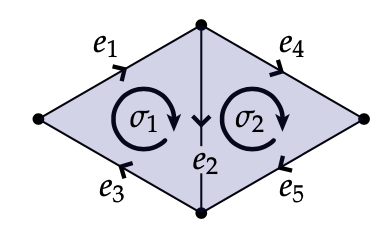
\includegraphics{images/Discrete_exterior_deriv_orientation.png}
    \end{figure}
    
    In the above figure, take $\pp_1$ to be the leftmost vertex and $\pp_2$ to be the topmost vertex. We have
    
    \begin{align*}
        (\hd\homega)_{\pp_1} &= \homega_1 + \homega_2 + \homega_3 \\
        (\hd\homega)_{\pp_2} &= \homega_4 + \homega_5 - \homega_1.
    \end{align*}
\end{example}

Before introducing the notion of \textit{mesh duality}, we need to know what a ``$k$-cell in $\R^n$'' is.

\begin{defn}
    ($k$-cell in $\R^n$).
    
    A \textit{$k$-cell in $\R^n$} is a subset of $\R^n$ that is a Cartesian product of $k$ closed intervals.
\end{defn}

\begin{defn}
    \scriptsize \cite{DDGArticle} \normalsize (Mesh duality).
    
    Consider a mesh $L$ (recall Definition \ref{ch::ddg::defn::mesh}). We will consider $L$ to be the ``original'', or \textit{primal mesh}. The \textit{dual mesh} to the primal mesh that is $L$ is obtained by replacing each $k$-simplex in $L$ with an $(n - k)$-cell. As stated in \cite{DDGArticle}, the dual mesh ``inherits several properties and operations'' from the primal mesh. ``Most important is the notion of incidence. For instance, if two primal edges are on the same primal face, then the corresponding dual faces are incident, that is, they share a common dual edge (which is the dual of the primal common face)''.
    
    Since a dual mesh is constructed out of $(n - k)$-cells rather than $(n - k)$-simplices, dual meshes are not necessarily simplicial complexes, but are instead examples of what are called \textit{cell complexes}. 
\end{defn}

\begin{defn}
    \scriptsize \cite{DDGNotes} \normalsize (Dual mesh conventions).

    The previous definition gives topological rules for constructing the dual complex, but it does not specify where the dual cells are located in space. As is done in \cite{DDGNotes}, ``we’ll choose the dual vertices to be located at the circumcenter of their primal face counterparts (circumcenter is the center of the circle that passes through all three triangle vertices)''. Doing this ensures that a dual edge is perpendicular to its corresponding primal edge.
\end{defn}

As it deals with relating $k$-dimensional space to $(n - k)$-dimensional space, the above definition is reminiscent of Hodge-duality. The Hodge-dual is indeed what will establish a correspondence between so-called \textit{primal discrete differential forms} and \textit{dual discrete differential forms}. 

\begin{defn}
\label{ch::ddg::defn::discrete_hodge_dual}
    \scriptsize \cite{DDGNotes} \normalsize (Discrete Hodge-duals)
    
    Let $K$ be a $2$-mesh embedded in $\C$. Denote the $2$-simplices (faces) of $K$ by $F_i$, the $1$-simplices (edges) of $K$ by $e_i$, and the $0$-simplices (vertices) of $K$ by $\pp_i$. We define the \textit{discrete Hodge-dual} $\hst$ on discrete primal differential forms in a piecewise manner:
    
    \begin{align*}
        (\hst \homega)_{F_i} &= \frac{1}{|F_i|} \homega, \quad \quad \text{$\homega$ is a discrete primal differential $2$-form}\\
        (\hst \homega)_{e_i} &= \frac{|e_i^*|}{|e_i|} \homega, \quad \quad \text{$\homega$ is a discrete primal differential $1$-form} \\
        (\hst \hf)_{\pp_i} &= |\pp_i^*| \homega, \quad \quad \text{$\hf$ is a discrete primal differential $0$-form (i.e. a function)}
    \end{align*}

    In the above, $|\cdot|$ takes the volume of its argument (so, in the above, it only ever returns $2$-dimensional area or the length of an edge), $e_i^*$ is the dual edge to $e_i$ (so $e_i^*$ is really a $1$-cell in the dual mesh), and $\pp_i^*$ is the dual vertex to $\pp_i$ (so $\pp_i^*$ is really a $2$-cell in the dual mesh).
    
    The middlemost definition of $\hst$ (which acts on a discrete primal differential $1$-form) is often referred to as the \textit{diagonal Hodge-dual}.
\end{defn}

\newpage

\section{Smoothing with the Laplacian}

In this section, our goal is to discretize the PDE

\begin{align*}
    \frac{\pd \FF}{\pd t} = \Delta \FF,
\end{align*}

where $M$ is a smooth $2$-manifold embedded in $\R^3$, $\FF:M \rightarrow \R^3$ is sufficently smooth, and where the \textit{Laplacian} operator $\Delta$ on vector-valued functions is defined as

\begin{align*}
    \Delta \FF = \Delta \begin{pmatrix} F_1 \\ F_2 \\ F_3 \end{pmatrix} := \begin{pmatrix} \Delta F_1 \\ \Delta F_2 \\ \Delta F_3 \end{pmatrix}.
\end{align*}

Here, the $\Delta$ on the right side of this definition is the Laplacian operator on scalar-valued functions, $\Delta = \div \circ \grad$.

It can be shown that $\Delta \FF = 2H\hat{\nn}$, where $H$ is the mean curvature\footnote{There are various ways to measure the curvature of a surface at a point. The mean curvature is one of these ways.} and $\hat{\nn}$ is the unit normal (see \cite[p. 114]{book::DDG}). Thus $\FF$ satisfies the above PDE iff, one can stay on the surface by going in the direction of the normal at a point, with strength proportional to the mean curvature at that point. More briefly, solving the above PDE is a formal way to ``smooth out'' the surface $M$ parameterized by $\FF$.

In order to solve the PDE $\frac{\pd \FF}{\pd t} = \Delta \FF$, we will set $\GG := \Delta \FF$ and consider the more abstract problem of

\begin{align*}
    \Delta \FF
    =
    \begin{pmatrix} \Delta F_1 \\ \Delta F_2 \\ \Delta F_3 \end{pmatrix}
    =
    \begin{pmatrix} G_1 \\ G_2 \\ G_3 \end{pmatrix}
    =
    \GG.
\end{align*}

This problem further reduces to the problem $\Delta F_i = G_i$, that is,

\begin{align*}
    \Delta f = g,
\end{align*}

where $f, g:M \rightarrow \R$ are sufficiently smooth real valued functions on $M$. So, our goal has turned into discretizing the Laplacian $\Delta$ on scalar-valued functions.

\subsection*{Discretizing the Laplacian}

We present two approaches for turning the ``regular'' Laplacian operator $\Delta$ on scalar-valued fucntions into the discrete Laplacian operator $\hDelta$ on scalar valued functions. The relatively standard first approach is to use the \textit{finite element method}. The novel second approach utilizes discrete differential geometry.


\subsubsection*{Discretizing the Laplacian with the finite element method}

Consider the PDE

\begin{align*}
    \Delta f = g.
\end{align*}

The basic of the idea of the \textit{finite element method} is to consider ``approximate solutions'' to the PDE in question that are defined piecewise on finitely many regions, called \textit{elements}. The vector space of functions that are defined piecewise on elements is called the \textit{discrete approximation space}. The best \textit{approximate solution} is the function in the discrete approximation space that has the smallest normed \textit{residual}. The norm we use to measure ``normed residuals'' is induced by an inner product on the discrete approximation space.

For our particular problem, our functions are defined on a $2$-mesh $K$ embedded in $\R^3$ (recall Definition \ref{ch::ddg::defn::mesh}). We take the elements to be $2$-simplices on the mesh. Thus, our discrete approximation space is the vector space of sufficiently smooth functions that are defined piecewise on $2$-simplices. 

For the purpose of establishing a norm, we will use the \textit{$L^2$ inner product} $\langle \cdot, \cdot \rangle$ on functions in our discrete approximation space, defined by

\begin{align*}
    \langle f, g \rangle = \int_K fg.
\end{align*}

The residual of a function $h$ in our discrete approximation space is $\Delta h - g$. (The residual is the zero function when $h$ is a solution to the PDE). The normed residual of $h$ is $||\Delta h - g||$, where the norm $||\cdot||$ is induced by the $L^2$ inner product.

In the finite element method, one also makes use of a basis for the discrete approximation space. We will use the basis $\Phi = \{\phi_{\pp_i}\}_{i = 1}^n$ of \textit{hat functions}, where the hat function $\phi_{\pp_i}:K \rightarrow \R$ is defined to be $1$ at the vertex $\pp_i$ and $0$ everywhere else. 

%We will suppose that the minimal possible residual for this particular PDE is $0$. If this is the case, then the best approximation $\hbest$ in the discrete approximation space satisfies $||\Delta \hbest - g||^2 = \langle \Delta \hbest - g, \Delta \hbest - g \rangle = 0$. Since $\Delta \hbest - g$ is in the discrete approximation space, it can be expressed as a basis sum of the hat functions $\phi_{\pp_i}$. We expand the second $\Delta \hbest - g$ in the inner product $ \langle \Delta \hbest - g, \Delta \hbest - g \rangle$ and use linearity, and the fact that sums of nonnegative terms are zero only if all the terms are zero, to obtain that we must have $\langle \Delta \hbest - g, \phi_{\pp_i} \rangle = 0$ for all $i$. That is, the $L^2$ inner product of the residual of the best approximate solution with each hat function is zero.

To discretize the Laplacian operator $\Delta$, we determine the Laplacian of a function $h$ in the discrete approximation space by using the basis of hat functions. We need the following lemma before doing so.

\begin{lemma}
\label{ch::ddg::lemma:green_first_identity}
    (Green's first identity).
    
    Let $M$ be a smooth $2$-manifold embedded in $\R^3$. If $f, g:M \rightarrow \R$ are sufficiently smooth, then
    
    \begin{align*}
        \langle \Delta f, g \rangle = -\langle \nabla f, \nabla g \rangle + \langle \nabla f \cdot \hat{\nn}, g \rangle_\pd,
    \end{align*}
    
    where $\langle \cdot, \cdot \rangle_\pd$ is the $L^2$ inner product on the boundary $\pd K$, and where we've made use of the $L^2$ inner product on vector fields that is defined by
    
    \begin{align*}
        \langle \VV_1, \VV_2 \rangle := \int \VV_1 \cdot \VV_2,
    \end{align*}
    
    Here, $\VV_1 \cdot \VV_2$ denotes the function $\pp \mapsto \VV_1|_\pp \cdot \VV_2|_\pp$.
\end{lemma}

\begin{proof}
    In general, $d(f\omega) = df \wedge d\omega + fd\omega$. So $d(g * df) = dg \wedge *df + gd*df$. Integrate over $M$ and apply Stokes' theorem to the left side to obtain
    
    \begin{align*}
        \int_{\pd M} g * df = \int_M dg \wedge *df + \int_M g d*df.
    \end{align*}
    
    Another general fact is that $**\omega = -1^{k(n-k)} \omega$ (see \cite{HodgeStar} for a proof of this), so $**(d*df) = d*df$ (use $k = 3$, $n = 3$). That is, $(d*d)f = *(*d*d)f = * \Delta f$. So the above becomes
    
    \begin{align*}
        \int_{\pd M} g * df =  \int_M dg \wedge *df + \int_M g *\Delta f.
    \end{align*}
    
    This is the same as
    
    \begin{align*}
        \int_{\pd M} g*df = \langle dg, df \rangle + \langle g, \Delta f \rangle.
    \end{align*}
    
    Rearranging, we have
    
    \begin{align*}
        \langle \Delta f, g \rangle = - \langle df, dg \rangle + \int_{\pd M} g*df.
    \end{align*}
    
    To complete the proof, observe that $\langle df, dg \rangle = \langle \nabla f, \nabla g \rangle$, and that after identifying $dx^{\sigma(i)} \wedge dx^{\sigma(j)}$ in $*df$ with $\sgn(\sigma) \see_{\sigma(\{1, 2, 3\} - \{i, j\})}$, $*df$ becomes $\nabla f \cdot \hat{\nn}$.
\end{proof}

We are now ready to take the first step in computing a discretization of the Laplacian with the finite element method.

\begin{deriv}
\label{ch::ddg::deriv::discrete_laplacian_inner_prod_grad}
    (Discrete Laplacian in terms of $L^2$ inner products of gradients).
    
    Let $K$ be a $2$-mesh embedded in $\R^3$, and let $K_j$ be the $2$-simplices (the triangles) on $K$. Using the bilinearity of the inner product $\langle \cdot, \cdot \rangle$, we see the \textit{discretization (via the finite element method) $\hDelta$ of the Laplacian $\Delta$} satisfies

    \begin{align*}
        \langle \hDelta h, \phi_{\pp_i} \rangle 
        = \sum_j \langle \hDelta h, \phi_{\pp_i} \rangle_{K_j}.
    \end{align*}
    
    Applying Green's first identity to the argument of the sum yields
    
    \begin{align*}
        \langle \hDelta h, \phi_{\pp_i} \rangle = -\sum_j \langle \hnabla h, \hnabla \phi_{\pp_i} \rangle_{K_j} + \sum_j \langle \hat{\nn} \cdot \hnabla h, \phi_{\pp_i} \rangle_{\pd K_j}.
    \end{align*}
    
    If the mesh has no boundary, then the inner product on the boundary $\langle \cdot, \cdot \rangle_{\pd K_j}$ vanishes, and we're left with
    
    \begin{align*}
        \langle \hDelta h, \phi_{\pp_i} \rangle = -\sum_j \langle \hnabla h, \hnabla \phi_{\pp_i} \rangle_{K_j}
        = - \langle \hnabla h, \hnabla \phi_{\pp_i} \rangle.
    \end{align*}
    
    Expanding $h$ in the basis $\Phi = \{\phi_{\pp_i}\}_{i = 1}^n$ as $h = \sum_j ([h]_\Phi)_j \phi_{\pp_j}$, using the linearity of $\hnabla$, and using the bilinearity of $\langle \cdot, \cdot \rangle$, we have
    
    \begin{align*}
         \langle \hDelta h, \phi_{\pp_i} \rangle =
         \langle \hnabla \Big( \sum_j ([h]_\Phi)_j \phi_{\pp_j} \Big), \hnabla \phi_{\pp_i} \rangle
         = \sum_j ([h]_\Phi)_j \langle \hnabla \phi_{\pp_j}, \hnabla \phi_{\pp_i} \rangle.
    \end{align*}
\end{deriv}

So it remains to compute $\langle \hnabla \phi_{\pp_j}, \hnabla \phi_{\pp_i} \rangle$. This will be accomplished by the next several lemmas.

\begin{lemma}
\label{ch::ddg:lemma::cotan_w_h_lemma}

    (Cotan formula lemma 1).
    
    The ``aspect ratio'' $\frac{w}{h}$ of a triangle is the sum of the cotangents of the interior angles at its base. That is,
    
    \begin{align*}
        \frac{w}{h} = \cot(\alpha) + \cot(\beta).
    \end{align*}
    
    \begin{figure}[H]
        \centering
        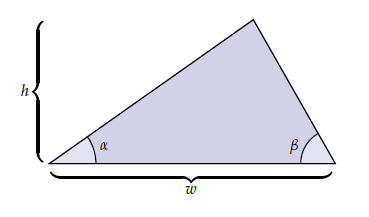
\includegraphics{images/fem_cotan_lemma1.PNG}
        \caption{\cite[p. 105]{book::DDG}}
    \end{figure}
\end{lemma}

\begin{proof}
    Drop an altitude from the top vertex of the triangle so that it intersects the base. Let $x$ denote the length from this intersection point to the right vertex of the triangle. Then $\cot(\alpha) = \frac{w - x}{h}$ and $\cot(\beta) = \frac{x}{h}$, so $\cot(\alpha) + \cot(\beta) = \frac{w}{h}$.
\end{proof}


\begin{lemma}
\label{ch::ddg:lemma::cotan_edge_perp}
    (Cotan formula lemma 2).
    
    If $\ee$ is the edge vector along the base of a triangle, and $\ee_\perp$ is the result of rotating $\ee$ counterclockwise by $\frac{\pi}{2}$, then the gradient of the hat function $\phi$ associated with the vertex opposite the side corresponding to $\ee$ is
    
    \begin{align*}
        \hnabla \phi  = \frac{\ee_\perp}{2A},
    \end{align*}
    
    where $A$ is the area of the triangle.
    
    \begin{figure}[H]
        \centering
        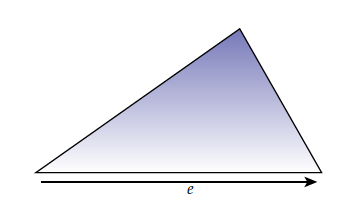
\includegraphics{images/fem_cotan_lemma2.PNG}
        \caption{\cite[p. 106]{book::DDG}}
    \end{figure}
\end{lemma}

\begin{proof}
%http://www.it.uu.se/edu/course/homepage/finmet2/vt14/material/Lab1.pdf
    Denote the left, top, and right vertices of the triangle by $\xx_i$, $i = 1, 2, 3$, respectively. Let $\phi = \phi_2$ denote the hat function associated with $\xx_2$, the top vertex. We have $\phi(\xx_1) = \phi(\xx_3) = 0$ and $\phi(\xx_2) = 1$.
    
    Since $\phi$ is linear, it is of the form $\phi(\xx) = \phi(\pp) + (\hnabla_\xx \phi)|_\pp \cdot (\xx - \pp)$, for any $\pp \in \R^3$. (Here, $\cdot$ is the dot product). It follows that the gradient of $\phi$ is the constant function $\hnabla_\xx \phi \equiv (\hnabla_\xx \phi)|_\pp$. Using $\pp = \xx_2$, we have
    
    \begin{align*}
        \phi(\xx) = 1 + (\hnabla_\xx \phi)|_{\xx_2} \cdot (\xx - \xx_2).
    \end{align*}
    
    Now use $\xx = \xx_1$ and $\xx = \xx_3$ to obtain
    
    \begin{align*}
        0 &= 1 + (\hnabla_\xx \phi)|_{\xx_2} \cdot (\xx_1 - \xx_2) \\
        0 &= 1 + (\hnabla_\xx \phi)|_{\xx_2} \cdot (\xx_3 - \xx_2).
    \end{align*}
    
    These equations are equivalent to
    
    \begin{align*}
        1 &= (\hnabla_\xx \phi)|_{\xx_2} \cdot (\xx_2 - \xx_1) \\
        1 &= (\hnabla_\xx \phi)|_{\xx_2} \cdot (\xx_2 - \xx_3).
    \end{align*}
    
    Subtract the second equation from the first and use the linearity of $\hnabla_\xx$ to obtain
    
    \begin{align*}
        (\hnabla_\xx \phi)|_{\xx_2} \cdot (\xx_3 - \xx_1) &= 0.
    \end{align*}
    
    Thus, $(\hnabla_\xx \phi)|_{\xx_2}$ is perpendicular to $\ee = \xx_3 - \xx_1$, which is the edge vector of the base of the depicted triangle. Since $(\hnabla_\xx \phi)|_{\xx_2}$ is the direction of  greatest \textit{increase}, not decrease, in $\phi$, then $(\hnabla_\xx \phi)|_{\xx_2}$ must point \textit{into} the triangle rather than out. ($\phi$ increases as we go ``into'' the triangle, since ${\phi(\xx_1) = \phi(\xx_3) = 0 < \phi(\xx_2) = 1}$). This implies that the direction of $(\hnabla_\xx \phi)|_{\xx_2}$ is the same as the direction of the $\ee_\perp$ described in the theorem. 
    
    To complete the proof, we will find the magnitude of $(\hnabla_\xx \phi)|_{\xx_2}$ and then show $\hnabla_\xx \phi \equiv (\hnabla_\xx \phi)|_{\xx_2} = \frac{\ee_\perp}{2A}$.
    
    Consider the previous equation
    
    \begin{align*}
        1 &= (\hnabla_\xx \phi)|_{\xx_2} \cdot (\xx_2 - \xx_1).
    \end{align*}
    
    The dot product on the right side can be re-expressed as
    
    \begin{align*}
        1 &= ||(\hnabla_\xx \phi)|_{\xx_2}|| \spc ||\xx_2 - \xx_1|| \cos \Big( \frac{\pi}{2} - \alpha \Big),
    \end{align*}
    
    where $\alpha$ is the angle between $(\hnabla_\xx \phi)|_{\xx_2}$ and $\xx_2 - \xx_1$. Equivalently, $\alpha$ is the angle between $\ee$ and the left side of the triangle. Using this reinterpretation of $\alpha$, we solve for $||(\hnabla_\xx \phi)|_{\xx_2}||$ and get
    
    \begin{align*}
        ||(\hnabla_\xx \phi)|_{\xx_2}|| 
        = \frac{1}{||\xx_2 - \xx_1|| \cos\Big( \frac{\pi}{2} - \alpha \Big)}
        = \frac{1}{||\xx_2 - \xx_1|| \sin(\alpha)} = \frac{1}{h},
    \end{align*}
    
    where $h$ is the height of the triangle. 
    
    Putting everything together, and using that $||\ee_\perp|| = ||\ee||$, we have
    
    \begin{align*}
        \hnabla_\xx \phi \equiv (\hnabla_\xx \phi)|_{\xx_2} 
        = ||(\hnabla_\xx \phi)|_{\xx_2}|| \hat{\ee}_\perp 
        = ||(\hnabla_\xx \phi)|_{\xx_2}|| \frac{\ee_\perp}{||\ee_\perp||}
        = \frac{1}{h ||\ee||} \ee_\perp
        = \frac{1}{2(\frac{1}{2} h ||\ee||)} \ee_\perp
        = \frac{\ee_\perp}{2A}.
    \end{align*}
    
    
    %Denote the hat functions associated with these vertices by $\phi_{\pp_i}$, $i = 1, 2, 3$, and suppose $\phi_{\pp_i}(x, y) = a_i + b_ix + c_iy$ for some constants $a_i, b_i, c_i$. By definition of the notion of ``hat function'', we have $\phi_{\pp_i}(\xx_j) = \delta^i_j$, so $a_i, b_i, c_i$ are determined as
    
    %\begin{align*}
    %    \begin{pmatrix}
    %        1 & x_1 & y_1 \\
    %        1 & x_2 & y_2 \\
    %        1 & x_3 & y_3
    %    \end{pmatrix}
    %    \begin{pmatrix} a_i \\ b_i \\ c_i \end{pmatrix}
    %    =
    %    \see_i,
    %\end{align*}
    
    %where $\see_i \in \R^3$ is the $i$th standard basis vector for $\R^3$. 
    
    %We are interested in the hat function $\phi = \phi_2$ corresponding to the top vertex. Solving the above system, we find

    %\begin{align*}
    %    \phi(x, y) = \frac{1}{2A}\Big( (x_3 y_1 - x_1 y_3 ) + (y_3 - y_1)x + (x_1 - x_3)y \Big),
    %\end{align*}
    
    %where $A = x_1(y_2 - y_3) + x_2(y_3 - y_1) + x_3(y_1 - y_2)$ is the area of the triangle.
    
    %We have $\nabla \phi = \frac{1}{2A} \begin{pmatrix} y_3 - y_1 \\ x_1 - x_3 \end{pmatrix}$. Since a counterclockwise rotation by $\frac{\pi}{2}$ sends $\begin{pmatrix} x \\ y \end{pmatrix} \mapsto \begin{pmatrix} -y \\ x \end{pmatrix}$, then
    
    %\begin{align*}
    %    \nabla \phi = 
    %    \frac{1}{2A} \begin{pmatrix} y_3 - y_1 \\ x_1 - x_3 \end{pmatrix} 
    %    = \RR_{\frac{\pi}{2}} \Big( \frac{1}{2A} \begin{pmatrix} x_3 - x_1 \\ y_3 - y_1 \end{pmatrix} \Big) 
    %    = \RR_{\frac{\pi}{2}} \Big( \frac{1}{2A}(\xx_3 - \xx_1) \Big) 
    %    = \RR_{\frac{\pi}{2}} \Big( \frac{1}{2A} \ee \Big)
    %    = \frac{\ee_\perp}{2A} 
    %\end{align*}

\end{proof}

\begin{lemma}
\label{ch::ddg::lemma::cotan_3}
    (Cotan formula lemma 3).
    
    The $L^2$ inner product of the gradient of a hat function $\phi$ corresponding to some vertex is
    
    \begin{align*}
        \langle \hnabla \phi, \hnabla \phi \rangle = \frac{1}{2} \Big(\cot(\alpha) + \cot(\beta) \Big),
    \end{align*}
    
    where $\alpha$ and $\beta$ are the interior angles at the other two vertices.
    
    \begin{figure}[H]
        \centering
        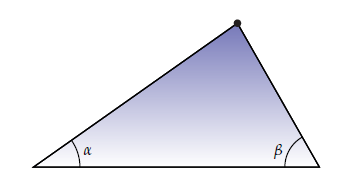
\includegraphics{images/fem_cotan_lemma3.PNG}
        \caption{\cite[p. 106]{book::DDG}}
    \end{figure}
\end{lemma}

\begin{proof}
    %\url{https://graphics.stanford.edu/courses/cs468-13-spring/assets/lecture12-lu.pdf}
    
    We have
    
    \begin{align*}
        \langle \hnabla \phi, \hnabla \phi \rangle
        = \int_{\text{triangle}} (\hnabla \phi) \cdot (\hnabla \phi)
        = \int_{\text{triangle}} ||\hnabla \phi||^2
        = A ||\hnabla \phi||^2,
    \end{align*}
    
    where $A$ is the area of the triangle. In the proof of the previous theorem, we showed $||\hnabla \phi|| = \frac{1}{h}$, where $h$ is the height of the triangle. So
    
    \begin{align*}
        \langle \hnabla \phi, \hnabla \phi \rangle
        = \frac{A}{h^2} 
        = \frac{\frac{1}{2}||\ee||h}{h^2} 
        = \frac{1}{2} \frac{||\ee||}{h}.
    \end{align*}
    
    Apply Lemma \ref{ch::ddg:lemma::cotan_w_h_lemma}, which states that the width-height ratio $\frac{||\ee||}{h}$ is $\frac{||\ee||}{h} = \cot(\alpha) + \cot(\beta)$, to obtain the result.
\end{proof}

\begin{lemma}
\label{ch::ddg::lemma::cotan_4}
    (Cotan formula lemma 4).
    
    Consider the hat functions $\phi_{\pp_i}$ and $\phi_{\pp_j}$ corresponding to vertices $\pp_i$ and $\pp_j$ of the same triangle. We have
    
    \begin{align*}
        \langle \hnabla \phi_{\pp_i}, \hnabla \phi_{\pp_j} \rangle = - \frac{1}{2} \cot(\theta),
    \end{align*}
    
    where $\theta$ is the angle between opposing edge vectors.
    
    \begin{figure}[H]
        \centering
        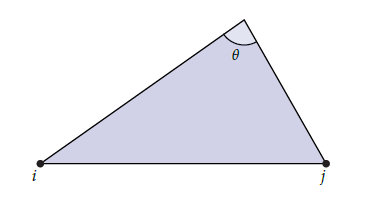
\includegraphics{images/fem_cotan_lemma4.PNG}
        \caption{\cite[p. 106]{book::DDG}}
    \end{figure}
\end{lemma}

\begin{proof}
    We have
    
    \begin{align*}
        \langle \hnabla \phi_{\pp_i}, \hnabla \phi_{\pp_j} \rangle
        = \int_{\text{triangle}} (\hnabla \phi_{\pp_i}) \cdot (\hnabla \phi_{\pp_i})
        = A (\hnabla \phi_{\pp_i}) \cdot (\hnabla \phi_{\pp_i}),
    \end{align*}
    
    where $A$ is the area of the triangle. Applying Lemma \ref{ch::ddg:lemma::cotan_edge_perp}, we have $\hnabla \phi_{\pp_i} = \frac{(\ee_{\pp_i})_\perp}{2A}$ and $\hnabla \phi_{\pp_j} = \frac{-(\ee_{\pp_j})_\perp}{2A}$, so
    
    \begin{align*}
        \langle \hnabla \phi_{\pp_i}, \hnabla \phi_{\pp_j} \rangle
        = A \frac{(\ee_{\pp_i})_\perp}{2A} \cdot \frac{-(\ee_{\pp_j})_\perp}{2A}
        = -\frac{\ee_{\pp_i} \cdot \ee_{\pp_j}}{4A}
        = -\frac{||\ee_{\pp_i}|| ||\ee_{\pp_j}|| \cos(\theta)}{4A}.
    \end{align*}
    
    To complete the proof, we do some trigonometry. Let $h$ be the height of the triangle, let $\alpha$ be the angle at vertex $\pp_i$ and let $\beta$ be the angle at vertex $\pp_j$. Then
    
    \begin{align*}
        \langle \hnabla \phi_{\pp_i}, \hnabla \phi_{\pp_j} \rangle
        = -\frac{||\ee_{\pp_i}|| \spc ||\ee_{\pp_j}|| \cos(\theta)}{4A}
        = -\frac{\frac{h}{\sin(\beta)} \frac{h}{\sin(\alpha)} \cos(\theta)}{4(\frac{1}{2}wh)}
        = -\frac{h \cos(\theta)}{2w\sin(\alpha)\sin(\beta)}
    \end{align*}
    
    where $w$ is the length of the base of the triangle. From Lemma \ref{ch::ddg:lemma::cotan_w_h_lemma}, we know ${w = h(\cot(\alpha) + \cot(\beta))}$. Thus, the above becomes
    
    \begin{align*}
        \langle \hnabla \phi_{\pp_i}, \hnabla \phi_{\pp_j} \rangle
        &= -\frac{\cos(\theta)}{2(\cot(\alpha) + \cot(\beta))\sin(\alpha)\sin(\beta)}
        = -\frac{\cos(\theta)}{2 \Big( \frac{\cos(\alpha)}{\sin(\alpha)} + \frac{\cos(\beta)}{\sin(\beta)}\Big) \sin(\alpha)\sin(\beta)} \\
        &= - \frac{\cos(\theta)}{2(\cos(\alpha) \sin(\beta) + \cos(\beta) \sin(\alpha))} = -\frac{\cos(\theta)}{2\sin(\alpha + \beta)}.
    \end{align*}
    
    Since $\alpha + \beta = \theta$, we obtain the claimed result. 
\end{proof}

Recall, the purpose of these lemmas was to determine $\langle \phi_{\pp_i}, \phi_{\pp_j} \rangle$. We needed to determine $\langle \phi_{\pp_i}, \phi_{\pp_j} \rangle$ so that we can finish the computation from the end of Derivation \ref{ch::ddg::deriv::discrete_laplacian_inner_prod_grad}:

\begin{align*}
    \langle \hDelta h, \phi_{\pp_i} \rangle
     = \sum_j ([h]_\Phi)_j \langle \hnabla \phi_{\pp_j}, \hnabla \phi_{\pp_i} \rangle.
\end{align*}

Lemma \ref{ch::ddg::lemma::cotan_3} gives us a formula for $\langle \phi_{\pp_i}, \phi_{\pp_j} \rangle$ when $i = j$, and Lemma \ref{ch::ddg::lemma::cotan_4} gives us a formula for $\langle \phi_{\pp_i}, \phi_{\pp_j} \rangle$ when $i \neq j$. Plugging the results of these lemmas into the above sum, we obtain the following theorem.

\begin{theorem}
    (Cotan formula via FEM).
    
    \begin{align*}
        (\hDelta h)_{\pp_i} = \frac{1}{2} \sum_j \Big( \cot(\alpha_j) - \cot(\beta_j) \Big) (h|_{\pp_i} - h|_{\pp_j})
    \end{align*}
\end{theorem}

\subsubsection*{Discretizing the Laplacian with discrete differential geometry}

We now use discrete differential geometry to produce a nearly identitical discretization for the Laplacian (the $\hDelta$ derived in this section will differ from the $\hDelta$ derived with the finite element method by a scalar multiple).

\begin{defn}
    (Discrete Laplacian via discrete differential geometry).
    
    Let $K$ be a $2$-mesh embedded in $\R^3$. Since Theorem \ref{ch::diff_forms::thm::div_grad_curl_exterior_derivative} tells us that $\text{div}(\VV) = *d*\VV^\flat$ and $\text{grad}(f) = (df)^\sharp$, then the ``regular'' Laplacian must act on $f$ by $\Delta f = (*d*d)f$. Thus, the ``regular'' Laplacian is
    
    \begin{align*}
        \Delta = *d*d.
    \end{align*}
    
    This ``regular'' Laplacian is easily discretized- to discretize, we just put hats on the $*$'s and $d$'s! Formally, the \textit{discrete Laplacian (via discrete differential geometry)} is defined to be
    
    \begin{align*}
        \hDelta := \hst \spc \spc \ddual \spc \spc \hst \spc \spc \dprimal,
    \end{align*}
    
    where $\dprimal$ and $\ddual$ are the discrete exterior derivatives on the primal and dual meshes, respectively. Referring back to Definition \ref{ch::ddg::defn::discrete_hodge_dual}, we see that the rightmost $\hst$ must be the diagonal Hodge-dual and that the leftmost $\hst$ must be the inverse of the third definition of the Hodge-dual from Definition \ref{ch::ddg::defn::discrete_hodge_dual}.
\end{defn}

\begin{theorem}
    (Formula for the discrete Laplacian on a $2$-mesh embedded in $\R^3$).

    Let $K$ be a $2$-mesh embedded in $\R^3$, and consider a discrete differential $0$-form $\hf$ on $K$. Then 
    
    \begin{align*}
        \boxed
        {
            (\hDelta \hf)_{\pp_i} = (\hst \spc \ddual \spc \hst \spc \dprimal \spc \hf)_{\pp_i} = \frac{1}{|\pp_i^*|} \sum_j \frac{|e_{ij}^*|}{|e_{ij}|}(f|_{\pp_j} - f|_{\pp_i})
        }
    \end{align*}
    
    where $\pp_i^*$ is the $2$-cell in the dual mesh that is dual to the vertex $\pp_i$ in the primal mesh $K$.
\end{theorem}

\begin{proof}
    First, we evaluate $\hd \hf$ on an arbitrary edge extending from $\pp_i$; let $e_{ij}$ be the edge connecting vertices $\pp_i$ and $\pp_j$ that has the standard orientation of $\{\pp_i, \pp_j\}$ inherited from $\R^2$. To take the discrete exterior derivative $\dprimal$, we integrate along the single edge $e_{ij}$:
    
    \begin{align*}
        (\dprimal \hf)_{e_{ij}} = \int_{e_{ij}} df = \int_{\pd e_{ij}} f = f|_{\pp_j} - f|_{\pp_i}.
    \end{align*}
    
    Then, applying the diagonal Hodge-dual $\hst$, we have
    
    \begin{align*}
        (\hst \spc \dprimal \hf)_{e_{ij}} 
        = \frac{|e_{ij}^*|}{|e_{ij}|}(f|_{\pp_j} - f|_{\pp_i}).
    \end{align*}
    
    Here, $e_{ij}^*$ is the $1$-cell that is dual to the $1$-simplex (the edge) $e_{ij}$. 
    
    Next, we apply $\ddual$ to $\hst \spc \dprimal \hf$. To do so, we only have to observe that $\ddual(\hst \spc \dprimal \hf)$ will be evaluated at the $2$-cell $\pp_i^*$ in the dual mesh; Stokes' theorem for discrete differential forms (Theorem \ref{ch::ddg::thm::discrete_stokes}) takes care of the rest:
    
    %\begin{align*}
    %    (\ddual \spc \hst \spc \dprimal \spc \hf)_C = \int_C d(*df).
    %\end{align*}
    
    %The $*df$ in the integrand on the right side, $d(*df)$, can be thought of as the result of taking the hats and subscripts off of the symbols in ``$\hst \spc \dprimal \hf$''. This corresponds to going from discrete differential geometry to ``regular'' differential geometry. 
    
    %Using Stokes' theorem for discrete differential forms (recall Theorem \ref{ch::ddg::thm::discrete_stokes}), the integral becomes
    
    \begin{align*}
       (\ddual \spc \hst \spc \dprimal \spc \hf)_{\pp_i^*}
       = \sum_j \frac{|e_{ij}^*|}{|e_{ij}|}(f|_{\pp_j} - f|_{\pp_i}).
    \end{align*}
    
    The last Hodge-dual is the inverse of the third Hodge-dual presented in Definition \ref{ch::ddg::defn::discrete_hodge_dual}. Thus, applying the last Hodge-dual divides the previous result by the area of $|\pp_i^*|$, and we obtain the claimed result.
\end{proof}

We only need one more lemma to complete our discretization of the Laplacian with discrete differential geometry.

\begin{lemma}
    (Cotan formula lemma).
    
    \begin{figure}[H]
        \centering
        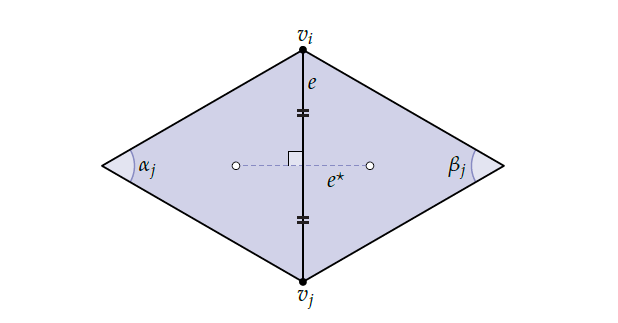
\includegraphics{images/DEC_cotan_formula.PNG}
        \caption{The diagram, which is from \cite[p. 110]{book::DDG}, uses $e$ and $e^*$ to denote $e_{ij}$ and $e_{ij}^*$.}
    \end{figure}
    
    Since Lemma \ref{ch::ddg:lemma::cotan_w_h_lemma} shows that the width-height ratio $\frac{2|e_{ij}^*|}{|e_{ij}|}$ is $\frac{2|e_{ij}^*|}{|e_{ij}|} = \cot(\alpha_j) + \cot(\beta_j)$, then
    
    \begin{align*}
        \frac{|e_{ij}^*|}{|e_{ij}|} = \frac{1}{2}(\cot(\alpha_j) + \cot(\beta_j)).
    \end{align*}
\end{lemma}

Combining the previous lemma and theorem, we obtain the following theorem, which finalizes our differential geometric discretization of the Laplacian.

\begin{theorem}
    (Cotan formula via discrete differential geometry).
    
    \begin{align*}
        \boxed
        {
            (\hDelta \hf)_{\pp_i} = \frac{1}{2 |\pp_i^*|} \sum_j \Big( \cot(\alpha_j) + \cot(\beta_j) \Big) (\hf|_{\pp_j} - \hf|_{\pp_i})
        }
    \end{align*}
    
\end{theorem}

\subsection*{Solving the problem}

We've seen that the discrete Laplacian can be expressed using the ``cotan formula'', and that this ``cotan formula'' can be derived using either the finite element method or with discrete differential geometry. How do we use this formula in a computer to smooth out surfaces in real time? The following theorem helps with this.

\begin{theorem}
    (Cotangent of the angle between vectors).
    
    Let $\vv_1, \vv_2 \in \R^3$, and consider the angle $\theta$ between $\vv_1$ and $\vv_2$. We have
    
    \begin{align*}
        \cot(\theta) = \frac{\vv_1 \cdot \vv_2}{||\vv_1 \times \vv_2||}.
    \end{align*}
\end{theorem}

\begin{proof}
    By definition of $\cot$, $\cot(\theta) = \frac{||(\vv_1)_{||}||}{||(\vv_1)_\perp||}$. Using Lemma \ref{ch::lin_alg::thm::vector_proj_dot_product}, we have $||(\vv_1)_{||}|| = ||\proj(\vv_1 \rightarrow \vv_2)|| = \frac{\vv_1 \cdot \vv_2}{||\vv_2||}$. Also, $||\vv_1 \times \vv_2|| = ||(\vv_1)_\perp|| ||\vv_2||$, so $||(\vv_1)_\perp|| = \frac{||\vv_1 \times \vv_2||}{||(\vv_1)_\perp||}$. Combining these two facts, we obtain $\cot(\theta) = \frac{(\vv_1 \cdot \vv_2)/||\vv_2||}{||\vv_1 \times \vv_2||/||\vv_2||}$, so $\cot(\theta) = \frac{\vv_1 \cdot \vv_2}{||\vv_1 \times \vv_2||}$.
\end{proof}

This theorem guarantees that if all lengths of all edges in our mesh are all the same, then the cotangent of the angle between any two edge vectors is a bilinear function. More specifically, since the cotangent produces a scalar, the cotangent of the angle between edges is a bilinear form in this situation. We learned in Chapter \ref{ch::bilinear_forms_metric_tensors} that a bilinear form can be identified with a $\binom{1}{1}$ tensor. Thus, provided that the edge lengths are all the same, we can produce a matrix which describes the action of the discrete Laplacian at each vertex.

\newpage

\section{Surface parameterization}

In this section, we explore how to wrap a $2$-dimensional map onto a $3$-dimensional surface (such as a globe) in an angle preserving manner\footnote{Our ``wrapping'' will not preserve lengths.}. Actually, instead of wrapping a $2$-dimensional map onto a $3$-dimensional surface, we will think about \textit{unwrapping} a $3$-dimensional surface into a flat $2$-dimensional map. That is, we will be considering smooth charts (recall Definition \ref{ch::manifolds::defn::chart}) on a $3$-dimensional manifold that map into a $2$-dimensional space.

Since we are dealing with the problem of angle-preservation, we will need to deal with rotations in the ``flat'' unwrapped domain. One easy way to deal with such $2$-dimensional rotations is to use the complex numbers $\C$, since multiplying by $i = \sqrt{-1}$ corresponds to performing a counterclockwise rotation by $\frac{\pi}{2}$ in the complex plane. Thus, given a smooth $2$-manifold $M$ embedded in $\C$, we will look for a global smooth chart $z:M \rightarrow \C$ that is angle preserving.

Before we proceed looking for such $z:M \rightarrow \C$, we need to define \textit{complex differential forms}.

\begin{defn}
    (Complex differential $k$-form).
    
    Earlier, we defined a \textit{real} differential $k$-form on a smooth manifold WWBOC $M$ to be a continuous function $\Lambda^k(T^*(M)) \rightarrow M$, where $\Lambda^k(T^*(M))$ is the subset of $T^0_k(T(M))$ consisting of antisymmetric tensors. These differential forms were \textit{real} in the sense that $T_\pp^*(M)$ was considered the double dual to the vector space $C^\infty(M \rightarrow \R)$. (This consideration ripples upwards because $T^*(M) := \bigsqcup_{\pp \in M} T_\pp^*(M)$).
    
    Let $M$ be a smooth manifold WWBOC. A \textit{complex} differential $k$-form on $M$ is a continuous function $\Lambda^k(T^*(M)) \rightarrow M$, where $\Lambda^k(T^*(M))$ is the subset of $T^0_k(T(M))$ consisting of antisymmetric tensors, and where $T_\pp^*(M)$ is considered as the double dual to the vector space $C^\infty(M \rightarrow \C)$.
    
    In practical terms, this definition implies the following analogue of Theorem \ref{ch::diff_forms::theorem::diff_form_in_chart}. Let $M$ be a smooth manifold WWBOC. Given any smooth chart $(U, \xx)$ on $M$, where $x^i$ is the $i$th component function of $\xx$, a complex differential $k$-form $\omega$ can be expressed as

    \begin{align*}
        \omega = \sum_{1 \leq i_1 < ... < i_k \leq n} (f_{i_1...i_k} + i g_{i_1 ... i_k}) dx^{i_1} \wedge ... \wedge dx^{i_k},
    \end{align*}
    
    where each $f_{i_1...i_k}, g_{i_1...i_k}:U \rightarrow \R$.
\end{defn}

Now that we have defined complex differential forms, we are able to speak of the differential of a complex-valued function. This is necessary for formally defining what it means for a chart on a smooth $2$-manifold embedded in $\C$ to preserve angles.

\begin{defn}
    (Angle-preserving complex chart).
    
    Let $M$ be a smooth $2$-manifold embedded in $\C$. A chart $z:M \rightarrow \C$ is \textit{angle-preserving} iff the following condition is satisfied:
    
    \begin{align*}
        \hat{\nn} \times dz(v_\pp) = i dz(v_\pp) \text{ for all $v_\pp \in T_\pp(M)$}.
    \end{align*}
    
    The left side is the result of pushing forward a tangent vector with the differential of $z$ and then rotating that tangent vector counterclockwise by $\frac{\pi}{2}$. The right side is the same thing, but the rotation has just been expressed using multiplication by $i$ rather than with a cross product.
\end{defn}

We now turn the above condition into one that is stated in terms of differential geometric concepts. This is accomplished by the following theorem, definition, and theorem.

\begin{theorem}
    (Cauchy-Riemann equation).

    Let $M$ be as in the previous definition, and suppose $z:M \rightarrow \C$ is angle-preserving. Notice that instead of pushing $v_\pp$ forward by $dz$ and then rotating with the cross product, we could have rotated and \textit{then} pushed forward $v_\pp$ with $dz$. More formally, there must be some $J:T_\pp(M) \rightarrow T_\pp(M)$ for which $\hat{\nn} \times d\FF(v_\pp) = d\FF(J(v_\pp))$. Thus, the definition of an angle preserving chart is equivalent to

    \begin{align*}
        dz(J(v_\pp)) = idz(v_\pp) \text{ for all $v_\pp \in T_\pp(M)$}.
    \end{align*}
    
    This equation is known as the \textit{Cauchy-Riemann equation}.
\end{theorem}

To obtain a differential geometric statement of the Cauchy-Riemann equation, we need to define the \textit{complex Hodge-dual}, which acts on complex differential forms.

\begin{defn}
    (Complex Hodge-dual).

    Let $M$ be a smooth $2$-manifold embedded in $\C$, and consider complex differential forms on $M$. We define the complex Hodge-dual $*$ to act on complex differential $1$- and $2$- forms, as follows. To specify the action of the complex Hodge-dual, we treat differential forms as objects that, pointwise, are functions. (Recall Derivation \ref{ch::diff_forms::deriv::diff_forms_actual_fns}).
    
    Let $v_\pp$ be any tangent vector with\footnote{Since the smooth $2$-manifolds we are considering are embedded in $\C$, their tangent spaces at any point can be identified with $\C$. The length of a tangent vector is then computed using the norm induced by the analogue of the dot product for $\C$. See example \ref{ch::ddg::example::complex_dot_prod}.} unit length.
    
    \begin{align*}
        &*\omega(v_\pp) := \omega(J(v_\pp)), \quad \text{$\omega$ is a complex differential $1$-form} \\
        &*\omega := \omega(v_\pp, J(v_\pp)), \quad \text{$\omega$ is a complex differential $2$-form}
    \end{align*}
    
    As a sanity check, note that the complex Hodge-dual of a complex differential $1$-form is a complex differential $(2 - 1 = 1)$-form, and the complex Hodge-dual of a complex differential $2$-form is a complex differential $(2 - 2 = 0)$-form.
\end{defn}

We can now present our final restatement of the angle-preservation condition.

\begin{theorem}
    (Cauchy-Riemann with the Hodge-dual).

     Let $M$ be a smooth $2$-manifold embedded in $\C$. The Cauchy-Riemann equation is
     
     \begin{align*}
        dz(J(v_\pp)) = idz(v_\pp) \text{ for all $v_\pp \in T_\pp(M)$}.
    \end{align*}
    
    The left side can be written as a contraction: $dz(J(v_\pp)) = C(dz, J(v_\pp))$. Using the previous definition of the complex Hodge-dual, we have $C(dz, J(v_\pp)) = C(*dz, v_\pp)$. Then, converting back to evaluation by the differential, we have $C(*dz, v_\pp) = *dz(v_\pp)$. Thus, the above is
    
    so the above becomes
    
    \begin{align*}
        *dz(v_\pp) = idz(v_\pp) \text{ for all $v_\pp \in T_\pp(M)$}.
    \end{align*}
    
    So the Cauchy-Riemann equation is equivalent to
    
    \begin{align*}
        \boxed
        {
            *dz = idz
        }
    \end{align*}
\end{theorem}

Having successfully translated the condition for angle-preservation into differential geometric terms, we will now find charts $z:M \rightarrow \C$ that ``almost'' solve the Cauchy-Riemann equation; we find charts that are as close to angle-preserving as possible.

Just as we did in our brief encounter with the finite element method, we will minimize the normed residual $||*dz - idz||$ of a chart $z:M \rightarrow \C$ to produce the chart which fails to solve the Cauchy-Riemann equation with by the smallest margin. (This time, we will not assume that the minimum such ``margin'' is zero, however).

To do this, we need to define an inner product, so that we can use its induced norm $||\cdot||$. Since we are working with complex numbers, we will actually be defining a \textit{Hermitian inner product}, which is similar to but not exactly the same as a ``regular'' inner product.

\begin{defn}
    (Hermitian inner product).
    
    Let $V$ be a vector space over $\C$. A \textit{Hermitian inner product} on $V$ is a binary function $\langle \cdot, \cdot \rangle:V \times V \rightarrow \C$ satisfying the following properties:
    
    \begin{enumerate}
        \item $\langle \cdot, \cdot \rangle$ respects addition. That is...
        \begin{enumerate}
            \item $\langle \vv_1 + \vv_2, \vv \rangle = \langle \vv_1, \vv \rangle + \langle \vv_2, \vv \rangle$ for all $\vv, \vv_1, \vv_2 \in V$.
            \item $\langle \vv, \vv_1 + \vv_2 \rangle = \langle \vv, \vv_1 \rangle + \langle \vv, \vv_2 \rangle$ for all $\vv, \vv_1, \vv_2 \in V$.
        \end{enumerate}
        \item $\langle c \vv_1, \vv_2 \rangle = c \langle \vv_1, \vv_2 \rangle$ for all $\vv_1, \vv_2 \in V$ and $c \in \C$.
        \item $\langle \vv_1, c \vv_2 \rangle = \cj{c} \langle \vv_1, \vv_2 \rangle$ for all $\vv_1, \vv_2 \in V$ and $c \in \C$.
        \item $\langle \vv_1, \vv_2 \rangle = \cj{\langle \vv_2, \vv_2 \rangle}$ for all $\vv_1, \vv_2 \in V$.
        \item $\langle \cdot, \cdot \rangle$ is positive-definite. That is, for all $\vv \in V$, $\langle \vv, \vv \rangle \geq 0$, and $\langle \vv, \vv \rangle = \mathbf{0}$ iff $\vv = \mathbf{0}$.
    \end{enumerate}
\end{defn}

\begin{example}
\label{ch::ddg::example::complex_dot_prod}
    The traditional example of a Hermitian inner product on an $n$-dimensional vector space $V$ over $\C$ is following ``complex analogue'' of the dot product: $\langle \vv_1, \vv_2 \rangle := \sum_{i = 1}^n ([\vv_1])^i \cj{([\vv_2])^i}$.
\end{example}

We now define the Hermitian product on complex differential $1$-forms that we will use to measure the normed residual.

\begin{defn}
    (Hodge Hermitian inner product on complex differential $1$-forms).
    
    Let $M$ be a smooth $2$-manifold embedded in $\C$. The \textit{Hodge Hermitian inner product} $\dlangle \cdot, \cdot \drangle$ on complex differential $1$-forms is the Hermitian inner product defined as
    
    \begin{align*}
        \dlangle \omega, \eta \drangle := \text{Re} \int_M *\cj{\omega} \wedge \eta.
    \end{align*}
\end{defn}

\begin{proof}
    We will show that $\dlangle \cdot, \cdot \drangle$ is positive-definite. The other conditions are simple to check.
    
    Consider $*\cj{\omega} \twedge \omega(v_\pp, J(v_\pp))$. (Recall Derivation \ref{ch::diff_forms::deriv::diff_forms_actual_fns} for what it means to interpret a differential form as an object that is, pointwise, a function. Also recall that we use $\twedge$ rather than $\wedge$ for such differential forms). We have
    
    \begin{align*}
        *\cj{\omega} \twedge \omega(v_\pp, J(v_\pp))
        =
        \det 
        \begin{pmatrix}
            *\cj{\omega}(v_\pp) & \omega(v_\pp) \\
            *\cj{\omega}(J(v_\pp)) & \omega(J(v_\pp))
        \end{pmatrix}
        =
        \det 
        \begin{pmatrix}
            \cj{\omega}(J(v_\pp)) & \omega(v_\pp) \\
            \cj{\omega}(J^2(v_\pp)) & \omega(J(v_\pp))
        \end{pmatrix}.
    \end{align*}
    
    The last equality in the above line follows by applying the definition of the complex Hodge-dual. Then, since $J^2 = i \cdot i = -1$, we have
    
    \begin{align*}
       *\cj{\omega} \twedge \omega(v_\pp, J(v_\pp))
        =
        \det 
        \begin{pmatrix}
            \cj{\omega}(J(v_\pp)) & \omega(v_\pp) \\
            -\cj{\omega}(v_\pp) & \omega(J(v_\pp))
        \end{pmatrix}
        =
        \cj{\omega}(J(v_\pp)) \omega(J(v_\pp)) + \cj{\omega}(v_\pp) \omega(v_\pp).
    \end{align*}
    
    Overall, we have
    
    \begin{align*}
        *\cj{\omega} \twedge \omega(v_\pp, J(v_\pp))
        =
        \cj{\omega}(J(v_\pp)) \omega(J(v_\pp)) + \cj{\omega}(v_\pp) \omega(v_\pp).
    \end{align*}
    
    We claim that $\cj{\omega}(v_\pp) \omega(v_\pp) \geq 0$ for any $v_\pp$. If the claim is true, then the previous equation yields the condition
    
    \begin{align*}
        *\cj{\omega} \twedge \omega(v_\pp, J(v_\pp)) \geq 0, \text{with equality to zero only when $\omega = \mathbf{0}$}.
    \end{align*}
    
    (We have equality to zero only when $\omega = \mathbf{0}$ because a sum of nonnegative terms is zero only when all the terms are zero).
    
    If we have this condition, then we have proved $\dlangle \cdot, \cdot \drangle$ is positive-definite, as integration over $M$ ultimately resolves into the integral of $\cj{\omega} \twedge \omega(v_\pp, J(v_\pp))$.
    
    So, we must prove $\cj{\omega}(v_\pp) \omega(v_\pp) \geq 0$, where $\omega$ is a complex differential $1$-form. We can express $\omega$ and $\cj{\omega}$ in coordinates as
    
    \begin{align*}
        \omega &= h_1 dx^1 + h_2 dx^2 \\
        \cj{\omega} &= \cj{h_1} dx^1 + \cj{h_2} dx^2,
    \end{align*}
    
    where $h_1, h_2:M \rightarrow \C$ are smooth complex functions.
    
    We can directly compute $\cj{\omega} \twedge v_\pp(\omega, v_\pp)$ by using the above coordinate representations. Use the fact that $h_i \cj{h_i} = |h_i|^2$, where $|\cdot|$ denotes the norm defined by $|a + bi| = \sqrt{a^2 + b^2}$, to prove the claim.
\end{proof}

We now work towards a theorem that expresses the square of the normed residual, $||*dz - idz||^2$, in terms of the Laplacian $\Delta = -*d*d$. (So, this theorem will use a different sign convention for the Laplacian than was used in the previous section). We need a slew of lemmas to prove the theorem.

\begin{lemma}
     The complex Hodge-dual preserves this norm  induced by the Hodge Hermitian inner product $\dlangle \cdot, \cdot \drangle$. That is, for all complex differential $1$-forms $\omega$, we have $||*\omega|| = ||\omega||$.
\end{lemma}

\begin{proof}
    We defined the complex Hodge-dual by treating complex differential forms as objects that, pointwise, are functions. In this definition, the length of vectors input into a Hodge-dual'ed differential form were the same as the length of the vectors input to the original differential form. Since the norm induced by the Hodge Hermitian inner product is an integral involving $\omega$, and as an integral of a differential form can be interpreted as an integral of that differential form being evaluated on tangent vectors, this implies that the norm induced by the Hodge Hermitian inner product is invariant under $*$.
\end{proof}

\begin{lemma}
    (Green's first identity for complex differential $1$-forms).
    
    Let $M$ be a smooth $2$-manifold embedded in $\C$. If $f, g:M \rightarrow \C$ are smooth and the normal derivative of either $f$ or $g$ vanishes on the boundary, then
    
    \begin{align*}
        \dlangle df, dg \drangle = \dlangle \Delta f, g \drangle,
    \end{align*}
    
    where $\Delta = -*d*d$ is the Laplace operator on $0$-forms.
\end{lemma}

\begin{proof}
    From the proof of Lemma \ref{ch::ddg::lemma:green_first_identity}, we have
    
    \begin{align*}
        \int_{\pd M} g * df =  \int_M dg \wedge *df + \int_M g *\Delta f.
    \end{align*}
    
    The boundary term vanishes by assumption, so we have
    
    \begin{align*}
        0 = \int_M dg \wedge *df + \int_M g *\Delta f = -\int_M *df \wedge dg + \int_M (*\Delta f) g = -\dlangle df, dg \drangle + \dlangle \Delta f, g \drangle.
    \end{align*}
\end{proof}

\begin{lemma}
    Let $||\cdot||$ be the norm induced by the Hodge Hermitian inner product $\dlangle \cdot, \cdot \drangle$ on complex differential $1$-forms. We have
    
    \begin{align*}
        ||*dz - idz||^2 = 2 \Big( \dlangle \Delta z, z \drangle - i \int_M d\cj{z} \wedge dz \Big).
    \end{align*}
\end{lemma}

\begin{proof}
    If $\langle \cdot, \cdot \rangle$ is a Hermitian inner product, then $||z + w||^2 = \langle z + w, z + w \rangle = \langle z, z \rangle + \langle z, w \rangle + \langle w, z \rangle + \langle w, w \rangle = ||z||^2 + \langle z, w \rangle + \cj{\langle z, w \rangle} + ||w||^2 = ||z||^2 + 2\text{Re}(\langle z, w \rangle) + ||w||^2$. Applying this fact to our situation, we have $||*dz - idz||^2 = ||*dz||^2 + 2\text{Re} \dlangle *dz, -idz \drangle + ||dz||^2$. Next, we use $||*dz|| = ||dz||$ to obtain $||*dz - idz||^2 = 2(||dz||^2 + \dlangle *dz, -i dz \drangle)$. 
    
    To finish, first note that $||dz||^2 = \langle dz, dz \rangle = \langle \Delta z, z \rangle$ by Green's first identity for complex differential $1$-forms. We now handle $\dlangle *dz, -i dz \drangle$ to complete the proof. By definition, 
    
    \begin{align*}
        \dlangle *dz, -i dz \drangle = \text{Re} \int_M **\cj{dz} \wedge (- i dz).
    \end{align*}
    
    From the definition of complex Hodge-dual, $**dz = dz$. It's simple to check that $\cj{dz} = d\cj{z}$ (ultimately this is because $\cj{df} = d\cj{f}$ for a complex differential $0$-form $f$), so we have
    
    \begin{align*}
        \dlangle *dz, -i dz \drangle = \text{Re} \int_M d\cj{z} \wedge (- i dz) = -i \int_M d\cj{z} \wedge dz.
    \end{align*}
    
    This proves the theorem.
\end{proof}

\begin{lemma}
    Let $M$ be a smooth $2$-manifold embedded in $\C$. If $z:M \rightarrow \C$ is a complex differential $1$-form on $M$, then
    
    \begin{align*}
        A(z) = -\frac{i}{2} \int_M d \cj{z} \wedge dz.
    \end{align*}
    
    is the surface area of $M$.
\end{lemma}

\begin{proof}
    We need to show $-\frac{i}{2} d\cj{z} \wedge dz = dx \wedge dy$. We show the equivalent statement $d\cj{z} \wedge dz = -2i dx \wedge dy$:
    
     \begin{align*}
        d\cj{z} \wedge dz &= d(\cj{x + iy}) \wedge d(x + iy) = d(x - iy) \wedge d(x + iy) = (dx - idy) \wedge (dx + idy) \\
        &= dx \wedge dx + i  dx \wedge dy - i  dy \wedge dx + dy \wedge dy = i  dx \wedge dy - i  dy \wedge dx = 2i  dx \wedge dy.
    \end{align*}
\end{proof}

Finally, we are ready to present an expression for square of the normed residual, $||*dz - idz||^2$, in terms of the Laplacian $\Delta = -*d*d$.

\begin{theorem}
    Let $||\cdot||$ be the norm induced by the Hodge Hermitian inner product $\dlangle \cdot, \cdot \drangle$ on complex differential $1$-forms. We have

    \begin{align*}
        ||*dz - idz||^2 = 2\dlangle \Delta z, z \drangle - 4A(z),
    \end{align*}
    
    where $A(z)$ is the surface area of $M$, 
    
    \begin{align*}
        A(z) = -\frac{i}{2} \int_M d \cj{z} \wedge dz.
    \end{align*}
\end{theorem}

\begin{proof}
    Combine the previous lemma and theorem.
\end{proof}

Recall that $||*dz - idz||$ measures how much a map $z$ fails to be angle-preserving. We want to minimize $||*dz - idz||$, i.e., minimize $||*dz - idz||^2$, to produce charts which are as close as possible to being perfectly angle-preserving.

According to \cite[p. 126]{book::DDG}, the trick to solving this minimization problem is to pick appropriate constraints. We don't want to pick constraints that are too loose, and we don't want to pick constraints that are too rigid. An example of a constraint that is too rigid is that of fixing the boundary of $M$. Why is this constraint ``too rigid''? Well, since $d\cj{z} \wedge dz = d(\cj{z} dz)$, we can use Stokes' theorem to express $A(z)$ as an integral over the boundary:

\begin{align*}
    A(z) = -\frac{i}{2} \int_M d \cj{z} \wedge dz = -\frac{i}{2} \int_M d(\cj{z} dz) = -\frac{i}{2} \int_{\pd M} \cj{z} dz.
\end{align*}

If the boundary is fixed, then $A(z)$ is a constant, so minimizing $||*dz - idz||^2 = 2\dlangle \Delta z, z \drangle - 4A(z)$ is the same as minimizing $\dlangle \Delta z, z \drangle$. But $\dlangle \Delta z, z \drangle$ is positive and quadratic, so the minimum of $\dlangle \Delta z, z \drangle$ occurs when $\nabla z = \mathbf{0}$, i.e., when $\Delta z = \div(\nabla z) = 0$. The fix proposed by \cite{book::DDG} is to solve the following minimization problem:

\begin{align*}
    \min_z & ||*dz - idz|| \\
    \st &||z|| = 1 \text{ for all $z$} \\
    &\langle z, \mathbf{1} \rangle = 0 \text{ for all $z$}
\end{align*}

Since $\Delta$ can be shown to be a self-adjoint operator, the above minimization problem can be solved using eigenvalue methods. Once this minimization problem is solved, a map that is as close to angle-preserving as possible is obtained.

%\section{Vector field decomposition and design}

%\begin{itemize}
%    \item Define $\coker(\FF) := W - \im(\FF)$. Prove that $\coker(\FF) = \im(\FF)^\perp$.
%    \item Define chain complex to be a sequence of vector spaces and a sequence of linear maps
    
%    \begin{align*}
%        V_k \overset{\FF_{k - 1}}{\leftarrow} ... \overset{\FF_1}{\leftarrow} V_1
%    \end{align*}
    
%    for which $\FF_{i + 1} \circ \FF_{i} = \mathbf{0} \iff \im(\FF_{i + 1}) \subseteq \ker(\FF_i)$.
    
%    \item (Lemma). Cokernel is the kernel of the adjoint.
%    \item For a chain complex with two maps and three vector spaces we have $\im(\FF_1) \cap \im(\FF_2^*) = \{\mathbf{0}\}$, where $*$ denotes the adjoint, not the dual
%    \begin{itemize}
%        \item Prove by using the lemma and that $\FF_{i + 1} \circ \FF_{i} = \mathbf{0}$ for a chain complex
%    \end{itemize}
%    \item For a chain complex of two maps, $V = \im(\FF_1) \oplus \im(\FF_2^*) \oplus \Big( (\ker(\FF_2) - \im(\FF_1)) \bigcup \{\mathbf{0}\} \Big)$
%    \begin{itemize}
%        \item Use $(V_1 \bigcup V_2)^\perp = V_1^\perp \cap V_2^\perp$
%    \end{itemize}
%\end{itemize}

    
    \part{Appendices}
    \chapter{Appendix}

\section*{Function-input duality}

\begin{deriv}
\label{ch::appendix::deriv::function_input_duality}
    (Function-input duality).
    
    Let $X$ and $Y$ be sets, let $x \in X$, let $f:X \rightarrow Y$ be a function, and consider the expression $f(x)$.

    Typically, we think of $f$ as being applied to $x$ to produce the output $f(x)$. We can also think of $x$ as being applied to $f$, in some sense, to produce $f(x)$. In intuitive notation, we have $\text{``}x(f)\text{''} = f(x)$.

    To formalize the intuition, notice that for every $x \in X$ there is a function $F_x$ that itself takes a function $X \rightarrow Y$ as input and applies it to $x$; so, $F_x(f) = f(x)$. Since the function sending $x \mapsto F_x$ is a bijection, we can identify $x$ with $F_x$ and then think of $x$ as being applied to $f$ via the action of $F_x$ on $f$. The intuition thus formalizes as $\text{``}x(f)\text{''} = F_x(f) = f(x)$.

    We've successfully formalized the idea of applying inputs to functions, but there is still more insight to be had. If we define $X^* := \{\text{functions $X \rightarrow Y$}\}$, then we have $f \in X^*$ and $F_x \in (X^*)^* = X^{**}$. We've seen that $x \mapsto F_x$ is a bijection $X \rightarrow X^{**}$. Thus, $X$ and $X^{**}$ are ``the same'', in some sense, and we write $X \cong X^{**}$. On the other hand, there is no natural bijection between $X$ and $X^*$.

    Overall, the relationship between $X$, $X^*$, and $X^{**}$ is that elements of $X \cong X^{**}$ and $X^*$ act on each other. Since elements of $X^*$ cannot be naturally identified with elements $X$, yet can still act on elements of $X$, we call $X^*$ the \textit{dual set (to $X$)}. (We call $X^{**}$ the \textit{double dual set (to $X$)}).
\end{deriv}

\section*{Symmetric and orthogonal linear functions}

The only results from this appendix that are necessary to know are the conditions (3) and (4) of Definition \ref{ch::bilinear_forms_metric_tensors::defn::orthogonal_linear_fn} satisfied by an orthogonal linear function.

\begin{deriv}
\label{ch::appendix::defn::dual_transf_after_id}
    (The adjoint of a linear function with respect to a nondegenerate bilinear form).
    
    Let $V$ and $W$ be finite-dimensional vector spaces, let $B$ be a nondegenerate bilinear form on $V$ and $W$, and consider the musical isomorphisms $\flat_1:V \rightarrow W^{*}$ and $\flat_2:W \rightarrow V^{*}$ induced by $B$.
    
    There is an induced linear map $\ff^\dag:V \rightarrow W$, called the \textit{adjoint of $\ff$ (with respect to $B$)}, that is obtained by using the musical isomorphisms on the domain and codomain of the dual transformation $\ff^*:W^* \rightarrow V^*$. We define $\ff^\dag$ to be the unique map for which the following diagram commutes:
    
    \begin{center}
       % https://tikzcd.yichuanshen.de/#N4Igdg9gJgpgziAXAbVABwnAlgFyxMJZABgBpiBdUkANwEMAbAVxiRADUQBfU9TXfIRRkAjFVqMWbAOoA9AFTdeIDNjwEiI0mOr1mrRBwVK+awZvLi9Uw9O7iYUAObwioAGYAnCAFskZEBwIJC0QBjoAIxgGAAV+dSEQTywnAAscEF1JAxAAHVz3cIyeD28-RFCgpAAmanCo2PjzQ2S0jKz9Nnz3d2MSkC9ff2oqxABmOsjouLMNQwYYd3aJTsN8pycTAbKkCcDgxGquCi4gA
        \begin{tikzcd}
        V \arrow[d, "\flat_1"'] \arrow[r, "\ff^\dag"] & W \arrow[d, "\flat_2"] \\
        W^* \arrow[r, "\ff^*"']                & V^*        
        \end{tikzcd}
    \end{center}
    
    Thus, $\ff^\dag = \flat_2^{-1} \circ \ff^* \circ \flat_1$, or, equivalently, $\flat_2 \circ \ff^\dag = \ff^* \circ \flat_1$.
    
    Since $\flat_2 \circ \ff^\dag = \ff^* \circ \flat_1$, then $\ff^\dag(\vv_0)^{\flat_2} = \ff^*(\vv_0^{\flat_1})$. Using the definition of $\ff^*$ (recall Definition \ref{ch::motivated_intro::defn::dual_transf}), we have $\ff^\dag(\vv_0)^{\flat_2} = \vv_0^{\flat_1} \circ \ff$. This is the same\footnote{Here we've used $B(\cdot, \vv_2)$ to denote the function $\vv_1 \mapsto B(\vv_1, \vv_2)$.} as $B(\cdot, \ff^\dag(\vv_0)) = B(\vv_0, \cdot) \circ \ff$. After evaluating both sides of this most recent equation on $\vv_1 \in V$ and relabeling $\vv_0$ as $\vv_2$, we have:
    
    \begin{align*}
        B(\vv_1, \ff^\dag(\vv_2)) = B(\vv_2, \ff(\vv_1)) \text{ for all $\vv_1, \vv_2 \in V$}.
    \end{align*}
\end{deriv}

Replacing the bilinear form of the above derivation with an inner product, we see that when we have an inner product instead of an arbitrary nondegenerate bilinear form, then $\ff^\dag$ is uniquely characterized by the condition that $\langle \vv_1, \ff^\dag(\vv_2) \rangle = \langle \vv_2, \ff(\vv_1) \rangle$ for all $\vv_1, \vv_2 \in V$. We will use this condition as a means to characterize special classes of linear functions. Specifically, we consider linear functions $\ff$ for which $\ff = \ff^\dag$ and for which $\ff^\dag = \ff^{-1}$. Before investigating such linear functions, we quickly present a definition.

\begin{defn}
    (Transpose of a matrix).
    
    The \textit{transpose} of an $m \times n$ matrix $(a^i{}_j)$ is the $n \times m$ matrix $(a^j{}_i)$. The tranpose of a matrix $\AA$ is denoted $\AA^\top$.
\end{defn}

Now, we consider linear functions $\ff$ for which $\ff = \ff^\dag$ and for which $\ff^\dag = \ff^{-1}$.

\begin{defn} 
\label{ch::bilinear_forms_metric_tensors::defn::symmetric_linear_fn}
    (Symmetric linear function).

    Let $V$ be a vector space, consider a linear function $\ff:V \rightarrow V$. We define $\ff$ to be \textit{symmetric} iff the following equivalent conditions hold:
    
    \begin{enumerate}
        \item $\ff = \ff^\dag$.
        \item $\langle \ff(\vv_1), \vv_2 \rangle = \langle \vv_1, \ff(\vv_2) \rangle$ for all $\vv_1, \vv_2 \in V$.
        \item If $V$ is finite-dimensional and $\hU$ is an orthonormal basis of $V$, then the matrix of $\ff$ relative to $\hU$ is equal to its transpose: $[\ff(\hU)]_{\hU}^\top = [\ff(\hU)]_{\hU}$. (Matrices that are equal to their own transpose are called \textit{symmetric}).
    \end{enumerate}
\end{defn}
        
\begin{proof}
    \mbox{} We need to show that the conditions are indeed equivalent.
    \\ \indent ($1 \iff 2$).
    \\ \indent ($\implies$). Use $\ff = \ff^\dag$ with $\langle \vv_1, \ff^\dag(\vv_2) \rangle = \langle \vv_2, \ff(\vv_1) \rangle$. 
    \\ \indent ($\impliedby$). We have $\langle \ff(\vv_1), \vv_2 \rangle = \langle \vv_1, \ff(\vv_2) \rangle$ for all $\vv_1, \vv_2 \in V$ and $\langle \vv_1, \ff^\dag(\vv_2) \rangle = \langle \vv_2, \ff(\vv_1) \rangle$. Therefore $\langle \vv_1, \ff(\vv_2) \rangle = \langle \vv_1, \ff^\dag(\vv_2) \rangle$. Due to the cancelability of inner products (this follows from the positive-definiteness of inner products), we have $\ff(\vv_2) = \ff^\dag(\vv_2)$ for all $\vv_2 \in V$. So $\ff = \ff^\dag$. 

    ($2 \iff $ 3). 
    \\ \indent ($\implies$). If (2) is true, then the $j$th column of $[\ff(\hU)]_{\hU}$ is $[\ff(\huu_j)]_{\hU}$, so the $^i_j$ entry of $[\ff(\hU)]_{\hU}$ is $\langle \ff(\huu_j), \huu_i \rangle$. Similarly, the $^i_j$ entry of the matrix of $\ff^\dag$ relative to $\hU$ is $\langle 
    \ff^\dag(\huu_j), \huu_i \rangle$. Due to the condition on $\langle \cdot, \cdot \rangle$ induced by the identification $V \cong V^*$, we have $\langle \ff^\dag(\huu_j), \huu_i \rangle = \langle \huu_j, \ff(\huu_i) \rangle = \langle \ff^\dag(\huu_i), \huu_j \rangle$. But this is the $^j_i$ entry of $[\ff(\hU)]_{\hU}$, i.e., the $^i_j$ entry of $[\ff(\hU)]_{\hU}^{\top}$. Thus $[\ff(\hU)]_{\hU} = [\ff(\hU)]_{\hU}^{\top}$.
    \\ \indent ($\impliedby$). Let $\hU = \{\huu_1, ..., \huu_n\}$ be an orthonormal basis for $V$, and let the matrix $\AA$ of $\ff$ relative to $\hU$ satisfy $a_{ij} = a^j_i$. Since $a^i{}_j = \langle \ff(\huu_i), \huu_j \rangle$, then $\langle \ff(\huu_i), \huu_j \rangle = \langle \huu_i, \ff(\huu_j) \rangle$. Extend with multilinearity to obtain the conclusion.
\end{proof}

\begin{defn}
\label{ch::bilinear_forms_metric_tensors::defn::orthogonal_linear_fn}
    (Orthogonal linear function). 
    
    Let $V$ be a vector space over $K$ (where\footnote{This is a very technical condition, and not much attention should be paid to it. We require this so that $2 \neq 0$, which allows us to divide by $2$.} we have $K \neq \Z/2\Z$), consider a linear function $\ff:V \rightarrow V$. We define $\ff$ to be \textit{orthogonal} iff the following equivalent conditions hold:
    
    \begin{enumerate}
        \item $\ff^\dag = \ff^{-1}$.
        \item $\langle \ff(\vv_1), \vv_2 \rangle = \langle \vv_1, \ff^{-1}(\vv_2) \rangle$ for all $\vv_1, \vv_2 \in V$.
        \item $\ff$ preserves inner product: $\langle \vv_1, \vv_2 \rangle = \langle \ff(\vv_1), \ff(\vv_2) \rangle$ for all $\vv_1, \vv_2 \in V$.
        \item $\ff$ preserves length: $\langle \vv, \vv \rangle = \langle \ff(\vv), \ff(\vv) \rangle$ for all $\vv \in V$.
        \item $\ff$ preserves length and angle: $\langle \vv, \vv \rangle = \langle \ff(\vv), \ff(\vv) \rangle$ for all $\vv \in V$ and $\theta(\vv_1, \vv_2) = \theta(\ff(\vv_1), \ff(\vv_2))$ for all $\vv_1, \vv_2 \in V$.
        \item If $V$ is finite-dimensional and $\hU$ is an orthonormal basis of $V$, then the matrix $[\ff(\hU)]_{\hU}$ of $\ff$ relative to $\hU$ has orthonormal columns.
        \item If $V$ is finite-dimensional and $\hU$ is an orthonormal basis of $V$, then $[\ff(\hU)]_{\hU}^{-1} = [\ff(\hU)]_{\hU}^{\top}$.
    \end{enumerate}
\end{defn}
        
\begin{proof}
    We need to show that the conditions are indeed equivalent. To do so, we prove $(3) \iff (4) \iff (5)$ and then $(1) \iff (2) \iff (3) \iff (6) \iff (7)$. The proof of $(3) \iff (4) \iff (5)$ is essentially the same as the proof of Lemma \ref{ch::lin_alg::lemma::orthogonal_linear_fns_preserve_alg_dot_product}; just replace the dot product of that lemma with an inner product. So, it remains to show $(1) \iff (2) \iff (3) \iff (6) \iff (7)$:
    \mbox{} \\
        ($1 \iff 2$).
        \\ \indent ($\implies$). Use $\ff^\dag = \ff^{-1}$ with $\langle \vv_1, \ff^\dag(\vv_2) \rangle = \langle \vv_2, \ff(\vv_1) \rangle$.
        \\ \indent($\impliedby$). $\langle \vv_1, \ff^{-1}(\vv_2) \rangle = \langle \ff(\vv_1), \vv_2 \rangle$ by hypothesis, and $\langle \ff(\vv_1), \vv_2 \rangle = \langle \vv_1, \ff^\dag(\vv_2) \rangle$ by condition on $\langle \cdot, \cdot \rangle$ imposed by identifying $V \cong V^*$ for $\ff^\dag$. Thus $\langle \vv_1, \ff^{-1}(\vv_2) \rangle = \langle \vv_1, \ff^\dag(\vv_2) \rangle$.
        \\ ($2 \iff 3$). Setting $\vv_3 := \ff^{-1}(\vv_2)$ shows that ${(\langle \ff(\vv_1), \vv_2 \rangle = \langle \vv_1, \ff^{-1}(\vv_2) \rangle \text{ for all $\vv_1, \vv_2 \in V$})} \iff$ \\ ${(\langle \ff(\vv_1), \ff(\vv_3) \rangle = \langle \vv_1, \vv_3 \rangle \text{ for all $\vv_1, \vv_3 \in V$})}$.
        \\ ($3 \iff 6$). 
        \\ \indent $(\implies$). We have in particular that $\langle \ff(\huu_i), \ff(\huu_j) \rangle = \langle \huu_i, {\uu}_j \rangle$. Since $\hU$ is orthonormal, $\langle \huu_i, \huu_j \rangle = \delta^i{}_j$. Therefore $\langle \ff(\huu_i), \ff(\huu_j) \rangle = \delta^i{}_j$, so the columns $[\ff(\huu_i)]_{\hU}$ of the matrix of $\ff$ relative to $\hU$ are orthonormal.
        \\ \indent $(\impliedby)$. Since the columns $[\ff(\huu_i)]_{\hU}$ of the matrix of $\ff$ relative to $\hU$ are orthonormal, we have $\langle \ff(\huu_i), \ff(\huu_j) \rangle = \delta^i{}_j$. Extend with multilinearity to obtain the conclusion.
        \\ ($6 \iff 7$).
        \\ \indent $(\implies$). The $^i_j$ entry of $[\ff(\hU)]_{\hU} [\ff(\hU)]_{\hU}^\top$ is $(\text{$i$th row of $[\ff(\hU)]_{\hU}$}) \cdot (\text{$j$th column of $[\ff(\hU)]_{\hU}$})\top = (\text{$i$th row of $[\ff(\hU)]_{\hU}$}) \cdot (\text{$j$th row of $[\ff(\hU)]_{\hU}$}) = \langle \ff(\huu_i), \ff(\huu_j) \rangle = \delta^i{}_j$. Therefore $[\ff(\hU)]_{\hU} [\ff(\hU)]_{\hU}^\top = \II$. A similar argument shows $[\ff(\hU)]_{\hU}^\top [\ff(\hU)]_{\hU} = \II$.
        \\ \indent $(\impliedby)$. Reversing the logic of the forward direction, we know $\langle \ff(\huu_i), \ff(\huu_j) \rangle = \delta^i{}_j$. Therefore (3) is satisfied. Then we use $(3) \implies (6)$.
\end{proof}

    \include{ch::references}
    
    \bibliographystyle{alpha}
    \bibliography{biblio}
    
    The source that is most frequently used is \cite{book::SM}; this is a comprehensive reference for differential geometry and manifolds. Explanations in \cite{book::SM} are generally good, but results sometimes are not motivated in the best way, and connections between concepts are sometimes missed. Following \cite{book::SM}, we have used \cite{book::Hubbard} the second-most. The book \cite{book::Hubbard} possibly has the best motivation I have ever seen in a math book. The definition of the exterior derivative and proof of the generalized Stokes' theorem were adapted from \cite{book::Hubbard}.
    
\end{document}